\keywords{компьютеры, программирование, алгоритмы, Scheme, Лисп, учебный курс}
\title
{Харольд Абельсон⫽ Джеральд Джей Сассман⫽ при␣участии Джули Сассман}
{Структура и␣интерпретация⌇ компьютерных программ}
{Второе издание}
{cover}

\dedication{Эта книга посвящается, с␣уважением и␣восторгом,⌇ духу, который живёт внутри компьютера}

Я␣считаю, что чрезвычайно важно, чтобы мы, занимаясь информатикой, продолжали получать радость от общения с␣компьютером. С␣самого начала это было огромным удовольствием. Конечно, время от времени встревали заказчики, и␣через какое-то время мы стали серьёзно относиться к␣их жалобам. Нам стало казаться, будто мы на самом деле ответственны за успешное, безошибочное, идеальное использование этий машин. Я␣не␣думаю, что это так. Я␣считаю, что мы ответственны за то, чтобы расширять их рамки, указывать им новые направления и␣сохранять радость в␣доме. Я␣надеюсь, что информатика никогда не␣перестанет быть радостью. Прежде всего я надеюсь, что мы не␣превратимся в␣миссионеров. Не␣надо чувствовать себя продавцом Библий. Таких в␣мире и␣так достаточно. То, что вы знаете о␣программировании, могут выучить и␣другие. Не␣думайте, что лишь в␣ваших руках ключ к␣успешной работе с␣компьютерами. Что у␣вас, как я думаю и␣надеюсь, есть — это разум: способность увидеть в␣машине больше, чем вы видели, когда вас впервые к␣ней подвели, увидеть, что вы способны сделать её␣бóльшим.

\signature{Алан␣Дж. Перлис⫽ (1␣апреля 1922␣года — 7␣февраля 1990␣года)}
\eject

\l{foreword}
\h0{Предисловие}

Программированием занимаются учителя, генералы, диетологи, психологи и␣родители. Программированию подвергаются армии, ученики и␣некоторые виды обществ. При решении крупных задач приходится применять последовательно множество программ, бóльшая часть которых возникает прямо в␣процессе решения. Эти программы изобилуют деталями, относящимися к␣той конкретной задаче, которую они решают. Если␣же вы хотите оценить программирование как интеллектуальную деятельность особого рода, то вам следует обратиться к␣программированию компьютеров; читайте и␣пишите компьютерные программы — много программ. Не␣так уж важно, что́ будет в␣них написано и␣как они будут применяться. Важно то, насколько хорошо они работают и␣как гладко стыкуются с␣другими программами при создании ещё более крупных программ. Программист должен равно стремиться и␣к␣совершенству в␣деталях, и␣к␣соразмерности сложного целого. В␣книге, которую вы держите в␣руках, словом «программирование» мы будем обозначать прежде всего создание, выполнение и␣изучение программ, написанных на одном из диалектов языка \X{Лисп} и␣предназначенных для выполнения на цифровом компьютере. Использование Лиспа не␣ограничивает нас в␣том, чтó мы можем описать в␣наших программах,— лишь в␣способе записи программ.

Продвигаясь по материалу этой книги, мы будем встречаться с␣тремя группами явлений: человеческий разум, совокупности компьютерных программ и␣компьютер. Всякая компьютерная программа — это порождённая человеческим разумом модель реального либо умозрительного процесса. Эти процессы, возникающие из нашего опыта и␣мысли, многочисленны, сложны в␣деталях, и␣мы всегда понимаем их лишь частично. Редко бывает так, что компьютерные программы отображают их к␣нашему окончательному удовлетворению. Таким образом, хотя наши программы представляют собой тщательно сработанные дискретные совокупности символов, мозаики переплетённых функций, они непрерывно развиваются: мы изменяем их по мере того, как наше восприятие модели приобретает всё бо́льшую глубину, расширяется и␣обобщается, до тех пор, пока модель не␣достигнет, наконец, метастабильного состояния в␣рамках следующей модели, над которой нам предстоит биться. Радостное возбуждение, сопутствующее компьютерному программированию, происходит из постоянного раскрытия в␣голове и␣в␣компьютере всё новых выраженных в␣виде программ механизмов и␣из взрыва ощущений, который они порождают. Искусство выражает наши мечты. Компьютер исполняет их под видом программ!

При всей своей мощности, компьютер требователен и␣придирчив. Ему нужны корректные программы, и␣то, что мы хотим ему сказать, должно быть выражено точно в␣каждой мелочи. Как и␣при всякой другой работе с␣символами, мы убеждаемся в␣правильности программ через доказательство. Самому Лиспу можно сопоставить семантику (между прочим, тоже модель), и␣если функцию программы можно выразить, скажем, в␣терминах исчисления предикатов, то логические методы позволят нам вывести формальное доказательство её корректности. К␣сожалению, когда программы становятся большими и␣сложными, что с␣ними всегда и␣происходит, адекватность, непротиворечивость и␣корректность самих спецификаций становится предметом сомнений, так что большие программы редко сопровождаются полными формальными доказательствами корректности. Поскольку большие программы вырастают из малых, нам необходимо обзавестись арсеналом программных структур, в␣правильности которых мы можем быть уверены — их можно назвать идиомами — и␣научиться объединять их в␣структуры большего размера с␣помощью организационных методов, ценность которых также доказана. Эти методы подробно обсуждаются в␣книге, и␣их понимание существенно для участия в␣прометеевском предприятии под названием «программирование». Для умения создавать большие, значительные программы нет лучшего помощника, чем свободное владение мощными организационными методами. И␣наоборот: затраты, связанные с␣написанием больших программ, побуждают нас изобретать новые методы уменьшения веса функций и␣деталей, входящих в␣эти программы.

В␣отличие от программ, компьютеры должны повиноваться законам физики. Если мы хотим, чтобы они работали быстро — по нескольку наносекунд на смену состояния,— электроны в␣их цепях не␣должны проходить большие расстояния (более полуметра). При этом тесно сконцентрированные в␣пространстве приборы излучают тепло, которое нужно куда-то отводить: так развилось изысканное инженерное искусство, призванное находить равновесие между обилием функций и␣плотностью расположения устройств. Так или иначе, аппаратура всегда работает ниже того уровня, на котором мы␣бы хотели программировать. Процессы, посредством которых наши программы на Лиспе переводятся в␣«машинные» программы, сами являются абстрактными моделями, которые мы воплощаем в␣программах. Их изучение и␣реализация многое дают для понимания организационных методов, направленных на программирование произвольных моделей. Разумеется, так можно смоделировать и␣сам компьютер. Подумайте об этом: поведение мельчайшего переключателя моделируется квантовой механикой, которая описывается дифференциальными уравнениями, точное поведение которых фиксируется в␣численных приближениях, представленных в␣виде компьютерных программ, которые выполняются на компьютере, составленном из..!

Раздельное выделение трёх групп явлений — не␣просто вопрос тактического удобства. Хотя эти группы и␣остаются, как говорится, в␣голове, но, проводя это разделение, мы позволяем потоку символов между тремя группами двигаться быстрее. В␣человеческом опыте с␣этим потоком по богатству, живости и␣обилию возможностей сравнится разве что сама эволюция жизни. Отношения между разумом человека, программами и␣компьютером в␣лучшем случае метастабильны. Компьютерам никогда не␣хватает мощности и␣быстродействия. Каждый новый прорыв в␣технологии производства аппаратуры ведёт к␣появлению более масштабных программных проектов, новых организационных принципов и␣к␣обогащению абстрактных моделей. Пусть каждый читатель время от времени спрашивает себя: «А␣зачем, к␣чему всё это?» — только не␣слишком часто, чтобы удовольствие от программирования не␣сменилось застреванием в␣горько-сладкой философии.

Из␣тех программ, которые мы пишем, некоторые (но␣всегда меньше, чем хотелось␣бы) решают точные математические задачи, такие, как сортировка последовательности чисел или нахождение их максимума, проверка числа на простоту или вычисление квадратного корня. Такие программы называются алгоритмами, и␣об их оптимальном поведении известно довольно много, особенно в␣том, что касается двух важных параметров: времени выполнения и␣потребления памяти. Программист должен владеть хорошими алгоритмами и␣идиомами. Несмотря на то, что некоторые программы сопротивляются точной спецификации, в␣обязанности программиста входит оценивать их производительность и␣всё время пытаться её улучшить.

Лисп — ветеран, он используется уже около четверти века. Среди живых языков программирования старше него только \X{Фортран}. Эти два языка обслуживали нужды важных прикладных областей: Фортран — естественно-научных и␣технических вычислений, а␣Лисп — искусственного интеллекта. Обе эти области по-прежнему важны, а␣программисты, работающие в␣них, настолько привязаны к␣этим двум языкам, что Лисп и␣Фортран вполне могут остаться в␣деле ещё по крайней мере на четверть столетия.

Лисп изменяется. Scheme, его диалект, используемый в␣этой книге, развился из первоначального Лиспа и␣отличается от него в␣некоторых важных отношениях: в␣частности, используются статические области связывания переменных, а␣функции могут возвращать в␣качестве значений другие функции. По␣семантической структуре Scheme так␣же близка к␣\X{Алгол}у␣60, как и␣к␣ранним вариантам Лиспа. Алгол␣60, который уже никогда не␣будет живым языком, продолжает жить в␣генах Scheme и␣Паскаля. Пожалуй, трудно найти две более разные культуры программирования, чем те, что образовались вокруг этих двух языков и␣используют их в␣качестве штампа общения. Паскаль служит для построения пирамид — впечатляющих, захватывающих статических структур, создаваемых армиями, которые укладывают на места тяжёлые плиты. При помощи Лиспа порождаются организмы — впечатляющие, захватывающие динамические структуры, создаваемые командами, которые собирают их из мерцающих мириад более простых организмов. Организующие принципы в␣обоих случаях остаются одни и␣те␣же, за одним существенным исключением: программист, пишущий на Лиспе, располагает на порядок большей творческой свободой в␣том, что касается функций, которые он создаёт для использования другими. Программы на Лиспе населяют библиотеки функциями, которые оказываются настолько полезными, что они переживают породившие их приложения. Таким ростом полезности мы во многом обязаны списку — исконной лисповой структуре данных. Простота структуры списков и␣естественность их использования отражаются в␣удивительной общности функций. В␣Паскале обилие объявляемых структур данных ведёт к␣специализации функций, которая сдерживает и␣наказывает случайное взаимодействие между ними. Лучше иметь сто функций, которые работают с␣одной структурой данных, чем десять функций, работающих с␣десятью структурами. В␣результате пирамиде приходится неподвижно стоять тысячелетиями; организм␣же будет развиваться или погибнет.

Чтобы увидеть эту разницу, сравните подачу материала и␣упражнения в␣этой книге с␣тем, что вы найдёте в␣любом вводном тексте, авторы которого используют Паскаль. Не␣поддавайтесь ошибочному впечатлению, будто этот текст может усвоить лишь студент MIT — представитель специфической породы, которая только там и␣встречается. Нет, именно такова должна быть всякая серьёзная книга, посвящённая программированию на Лиспе, вне зависимости от того, где и␣кто по ней учится.

Учтите, что это текст о␣программировании, в␣отличие от большинства книг по Лиспу, которые используются для подготовки работников в␣области искусственного интеллекта. В␣конце концов, основные программистские заботы вычислительной инженерии и␣искусственного интеллекта стремятся к␣взаимопроникновению по мере того, как соответствующие системы увеличиваются в␣объёме. Это объясняет рост интереса к␣Лиспу за пределами искусственного интеллекта.

Как и␣можно было ожидать, глядя на цели, которые ставят перед собой исследователи в␣области искусственного интеллекта, область эта порождает множество значительных программистских задач. В␣других программистских культурах такой наплыв задач рождает новые языки. В␣самом деле, в␣любой большой программной задаче один из важных принципов организации состоит в␣том, чтобы ограничить и␣изолировать потоки информации в␣отдельных модулях задачи, изобретая для этого язык. По␣мере приближения к␣границам системы, где мы — люди — взаимодействуем чаще всего, эти языки обычно становятся всё менее примитивными. В␣результате такие системы содержат сложные функции по обработке языка, повторенные по многу раз. У␣Лиспа␣же синтаксис и␣семантика настолько просты, что синтаксический разбор можно считать элементарной задачей. Таким образом, методы синтаксического разбора не␣играют почти никакой роли в␣программах на Лиспе, и␣построение языковых процессоров редко служит препятствием для роста и␣изменения больших Лисп-систем. Наконец, именно эта простота синтаксиса и␣семантики возлагает бремя свободы на всех программистов на Лиспе. Никакую программу на Лиспе больше, чем в␣несколько строк длиной, невозможно написать, не␣населив её самостоятельными функциями. Находите новое и␣приспосабливайте, складывайте и␣стройте новыми способами! Наш тост — за программиста на Лиспе, укладывающего свои мысли во␣вложения скобок.

\signature{\Xp{Алан␣Дж. Перлис},⫽ Нью-Хейвен, Коннектикут}

\l{preface2}
\h0{Предисловие⌇ ко␣второму изданию}

\epigraph{Возможно␣ли, что программы не␣похожи ни␣на что другое, что они предназначены на выброс; что вся штука состоит в␣том, чтобы всегда видеть в␣них мыльный пузырь?}
{\Xp{Алан␣Дж. Перлис}}

Материал этой книги был основой вводного курса по информатике в␣MIT начиная с␣1980␣года. К␣тому времени, как было выпущено первое издание, мы преподавали этот материал в␣течение четырёх лет, и␣прошло ещё двенадцать лет до появления второго издания. Нам приятно, что наша работа была широко признана и␣включена в␣другие тексты. Мы видели, как наши ученики черпали идеи и␣программы из этой книги и␣на их основе строили новые компьютерные системы и␣языки. Буквально по старому талмудическому каламбуру, наши ученики стали нашими строителями. Мы рады, что у␣нас такие одарённые ученики и␣такие превосходные строители.

Готовя это издание, мы включили в␣него сотни поправок, которые нам подсказали как наш собственный преподавательский опыт, так и␣советы коллег из MIT и␣других мест. Мы заново спроектировали большинство основных программных систем в␣этой книге, включая систему обобщённой арифметики, интерпретаторы, имитатор регистровых машин и␣компилятор; кроме того, мы переписали все примеры программ так, чтобы любая реализация Scheme, соответствующая стандарту Scheme IEEE \bib{(IEEE 1990)}, была способна выполнять этот код.

Это издание особо выделяет несколько новых тем. Самая важная из них состоит в␣том, что центральную роль в␣вычислительных моделях играют различные подходы ко времени: объекты, обладающие состоянием, параллельное программирование, функциональное программирование, ленивые вычисления и␣недетерминистское программирование. Мы включили в␣текст новые разделы по параллельным вычислениям и␣недетерминизму и␣постарались интегрировать эту тему в␣материал книги на всём её протяжении.

Первое издание книги почти точно следовало программе нашего односеместрового курса в␣Массачусетском Технологическом институте (MIT). Рассмотреть весь материал, включая то, что добавлено во втором издании, в␣течение семестра будет невозможно, так что преподавателю придётся выбирать. В␣нашей собственной практике мы иногда пропускаем раздел про логическое программирование \r{logic-programming}{(раздел␣\n)}; наши студенты используют имитатор регистровых машин, но мы не␣описываем его реализацию \r{a-register-machine-simulator}{(раздел␣\n)}; наконец, мы даём лишь беглый обзор компилятора \r{compilation}{(раздел␣\n)}. Даже в␣таком виде курс остаётся интенсивным. Некоторые преподаватели предпочтут ограничиться первыми тремя или четырьмя главами, оставляя прочий материал для последующих курсов.

Сайт \E{World Wide Web} \uri{http://mitpress.mit.edu/sicp} предоставляет поддержку пользователям этой книги. Там есть программы из книги, простые задания по программированию, сопроводительные материалы и␣реализации диалекта Лиспа Scheme.

\l{preface1}
\h0{Предисловие к␣первому изданию}

\epigraph{Компьютер подобен скрипке. Представьте себе новичка, который сначала испытывает проигрыватель, затем скрипку. Скрипка, говорит он, звучит ужасно. Именно этот аргумент мы слышали от наших гуманитариев и␣специалистов по информатике. Компьютеры, говорят они, хороши для определённых целей, но они недостаточно гибки. Так␣же и␣со скрипкой, и␣с␣пишущей машинкой, пока вы не␣научились их использовать.}
{\Xp{Марвин Минский}.⫽ Почему программирование — хороший␣способ␣выражения малопонятных и␣туманно␣сформулированных идей}

«Структура и␣интерпретация компьютерных программ» — это вводный курс по информатике в␣MIT. Он обязателен для всех студентов MIT на специальностях «электротехника» и␣«информатика», как одна из четырёх частей «общей базовой программы обучения», которая включает ещё два курса по электрическим схемам и␣линейным системам, а␣также курс по проектированию цифровых систем. Мы принимали участие в␣развитии этого курса начиная с␣1978␣года и␣преподавали этот материал в␣его нынешней форме начиная с␣осени 1980␣года шестистам — семистам студентам в␣год. Большинство этих студентов не␣имела почти никакого или совсем никакого формального образования в␣области вычислительной техники, хотя у␣многих была возможность общения с␣компьютерами, а␣некоторые обладали значительным опытом в␣программировании либо в␣проектировании аппаратуры.

Построение этого вводного курса по информатике отражает две основные задачи. Во-первых, мы хотим привить слушателям идею, что компьютерный язык — это не␣просто способ заставить компьютер производить вычисления, а␣новое формальное средство выражения методологических идей. Таким образом, программы должны писаться для того, чтобы их читали люди, и␣лишь во вторую очередь для выполнения машиной. Во-вторых, мы считаем, что основной материал, на который должен быть направлен курс этого уровня,— не␣синтаксис определённого языка программирования, не␣умные алгоритмы для эффективного вычисления определённых функций, даже не␣математический анализ алгоритмов и␣оснований программирования, но методы управления интеллектуальной сложностью больших программных систем.

Наша цель — развить в␣студентах, проходящих этот курс, хороший вкус к␣элементам стиля и␣эстетике программирования. Они должны овладеть основными методами управления сложностью в␣большой системе, уметь прочитать 50-страничную программу, если она написана в␣хорошем стиле. Они должны в␣каждый данный момент понимать, чего сейчас не␣следует читать и␣что сейчас не␣нужно понимать. Они не␣должны испытывать страха перед модификацией программы, сохраняя при этом дух и␣стиль исходного автора.

Все эти умения ни␣в␣коем случае не␣исчерпываются компьютерным программированием. Методы, которым мы учим и␣из которых мы черпаем, одни и␣те␣же в␣любом техническом проектировании. Мы управляем сложностью с␣помощью построения абстракций, скрывающих, когда это нужно, детали. Мы управляем сложностью путём установления стандартных интерфейсов, которые позволяют нам строить системы из единообразных, хорошо понимаемых кусков способом «смеси и␣стыковки». Мы управляем сложностью с␣помощью построения новых языков для описания проекта, каждый из которых концентрирует внимание на определённых деталях проекта и␣уводит его от других.

В␣основе нашего подхода к␣предмету лежит убеждение, что информатика (computer science — компьютерная наука) не␣является наукой и␣что её значение мало связано с␣компьютерами. Компьютерная революция — это революция в␣том, как мы мыслим и␣как мы выражаем наши мысли. Сущность этих изменений состоит в␣появлении дисциплины, которую можно назвать \e{компьютерной эпистемологией},— исследования структуры знания с␣императивной точки зрения, в␣противоположность более декларативной точке зрения классических математических дисциплин. Математика даёт нам структуру, в␣которой мы можем точно описывать понятия типа «что есть». Вычислительная наука даёт нам структуру, в␣которой мы можем точно описывать понятия типа «как».

В␣преподавании мы используем диалект языка программирования Лисп. Мы не␣учим формальной стороне языка, поскольку в␣этом не␣возникает нужды. Мы просто его используем, и␣студенты схватывают его за несколько дней. В␣этом состоит одно из больших преимуществ лиспоподобных языков: в␣них очень мало способов строить составные выражения и␣нет почти никакой синтаксической структуры. Все формальные детали могут быть описаны за час, как правила шахмат. Спустя некоторое время мы забываем о␣формальных свойствах языка (поскольку их нет) и␣продолжаем говорить о␣настоящих вопросах; определяем, что именно мы хотим вычислить, ка́к мы будем разбивать задачу на куски разумного размера и␣ка́к потом будем работать с␣этими кусками. Ещё одно преимущество Лиспа состоит в␣том, что он поддерживает (но␣не␣навязывает) больше крупномасштабных стратегий разбиения программ на модули, чем любой другой известный нам язык. Можно строить абстракции процедур и␣данных, можно использовать функции высшего порядка, чтобы охватить общие шаблоны их использования, можно моделировать локальное состояние с␣использованием присваивания и␣изменения данных, можно связывать части программы с␣помощью потоков и␣отложенных вычислений, и␣можно с␣лёгкостью реализовывать встроенные языки. Всё это включено в␣диалоговое окружение с␣превосходной поддержкой пошагового проектирования, построения, тестирования и␣отладки программ. Мы благодарны всем поколениям Лисп-магов начиная с␣Джона Маккарти, которые создали замечательный инструмент непревзойдённой силы и␣красоты.

Scheme, тот диалект Лиспа, который мы используем, пытается совместить силу и␣красоту Лиспа и␣Алгола. От␣Лиспа мы берём метаязыковую мощь, которой он обязан простоте своего синтаксиса, единообразное представление программ как объектов данных, размещение данных в␣куче с␣последующей сборкой мусора. От␣Алгола мы берём лексическую область действия и␣блоковую структуру, подаренные нам первопроходцами проектирования языков программирования из комитета по Алголу. Мы хотим упомянуть Джона Рейнольдса и␣Питера Ландина, открывших связь Чёрчева лямбда-исчисления со структурой языков программирования. Мы также отдаём дань признательности математикам, разведавшим эту область за десятилетия до появления на сцене компьютеров. Среди этих первопроходцев были Алонзо Чёрч, Беркли Россер, Стивен Клини и␣Хаскелл Карри.

\l{acknowledgments}
\h0{Благодарности}

Мы хотели␣бы поблагодарить множество людей, которые помогли нам создать эту книгу и␣этот курс.

Наш курс — очевидный интеллектуальный потомок «6.321», замечательного курса по компьютерной лингвистике и␣лямбда-исчислению, который читали в␣MIT в␣конце 60-х Джек Уозенкрафт и␣Артур Эванс␣мл.

Мы очень обязаны Роберту Фано, который реорганизовал вводную программу MIT по электротехнике и␣информатике, сосредоточившись на принципах технического проектирования. Он вдохновил нас на это предприятие и␣написал первую программу курса, из которого развилась эта книга.

Стиль и␣эстетика программирования, которые мы пытаемся привить читателю, во многом были разработаны совместно с␣Гаем Льюисом Стилом␣мл., который вместе с␣Джеральдом Джеем Сассманом участвовал в␣первоначальной разработке языка Scheme. В␣дополнение к␣этому Дэвид Тёрнер, Питер Хендерсон, Дэн Фридман, Дэвид Уайз и␣Уилл Клингер научили нас многим из приёмов функционального программирования, которые излагаются в␣данной книге.

Джон Мозес научил нас структурировать большие системы. Благодаря его опыту с␣системой символьных вычислений \E{Macsyma} мы стали понимать, что необходимо избегать усложнённости структур управления и␣в␣первую очередь заботиться о␣такой организации данных, которая отражает реальную структуру моделируемого мира.

Марвин Минский и␣Сеймур Пэйперт сильно повлияли на формирование нашего подхода к␣программированию и␣к␣его месту в␣нашей интеллектуальной жизни. Благодаря им мы понимаем, что вычисление даёт нам средство выражения и␣исследования мыслей, которые иначе были␣бы слишком сложны, чтобы с␣ними можно было точно работать. Они подчёркивают, что способность писать и␣изменять программы даёт студенту мощное средство, с␣помощью которого исследование становится естественной деятельностью.

Кроме того, мы полностью согласны с␣Аланом Перлисом в␣том, что программирование — это огромное удовольствие и␣что нам нужно стараться поддерживать радость программирования. Часть этой радости приходит от наблюдения за работой великих мастеров. Нам выпало счастье быть учениками у␣ног Билла Госпера и␣Ричарда Гринблатта.

Трудно перечислить всех тех, кто принял участие в␣развитии программы нашего курса. Мы благодарим всех лекторов, инструкторов и␣преподавателей, которые работали с␣нами в␣прошедшие пятнадцать лет и␣потратили много часов сверхурочной работы на наш предмет, особенно Билла Сиберта, Альберта Мейера, Джо Стоя, Рэнди Дэвиса, Луи Брэйда, Эрика Гримсона, Рода Брукса, Линна Стейна и␣Питера Соловитца. Мы␣бы хотели особо отметить выдающийся педагогический вклад Франклина Турбака, который теперь преподаёт в␣Уэллсли: его работа по обучению младшекурсников установила стандарт, на который мы все можем равняться. Мы благодарны Джерри Сальтцеру и␣Джиму Миллеру, которые помогли нам бороться с␣тайнами параллельных вычислений, а␣также Питеру Соловитцу и␣Дэвиду Макаллестеру за их вклад в␣представление недетерминистских вычислений в␣\r{metalinguistic-abstraction}{главе␣\n}.

Много людей вложило немалый труд в␣преподавание этого материала и␣в␣других университетах. Вот некоторые из тех, с␣кем мы тесно общались в␣работе: это Джекоб Кацнельсон в␣Технионе, Хэрди Майер в␣Калифорнийском университете в␣Ирвине, Джо Стой в␣Оксфорде, Элиша Сэкс в␣университете Пердью и␣Ян Коморовский в␣Норвежском университете естественных и␣технических наук. Мы гордимся коллегами, которые получили награды за адаптацию этого предмета в␣других университетах: это Кеннет Йип в␣Йеле, Брайан Харви в␣Калифорнийском университете в␣Беркли и␣Дон Хаттенлохер в␣Корнелле.

Эл Мойе дал нам возможность прочитать этот материал инженерам компании Хьюлетт-Паккард и␣устроил производство видеоверсии этих лекций. Мы хотели␣бы поблагодарить одарённых преподавателей — в␣особенности Джима Миллера, Билла Сиберта и␣Майка Айзенберга,— которые разработали курсы повышения квалификации с␣использованием этих видеоматериалов и␣преподавали по ним в␣различных университетах и␣корпорациях по всему миру.

Множество работников образования проделали значительную работу по переводу первого издания. Мишель Бриан, Пьер Шамар и␣Андре Пик сделали французское издание, Сюзанна Дэниелс-Хэрольд выполнила немецкий перевод, а␣Фумио Мотоёси — японский. Мы не␣знаем авторов китайского издания, однако считаем для себя честью быть выбранными в␣качестве объекта «неавторизованного» перевода.

Трудно перечислить всех людей, внёсших технический вклад в␣разработку систем программирования на языке Scheme, которые мы используем в␣учебных целях. Кроме Гая Стила, в␣список важнейших магов входят Крис Хансон, Джо Боубир, Джим Миллер, Гильермо Росас и␣Стивен Адамс. Кроме них, существенное время и␣силы вложили Ричард Столлман, Алан Боуден, Кент Питман, Джон Тафт, Нил Мэйл, Джон Лэмпинг, Гуин Оснос, Трейси Ларраби, Джордж Карретт, Сома Чаудхури, Билл Киаркиаро, Стивен Кирш, Лей Клотц, Уэйн Носс, Тодд Кэсс, Патрик О’Доннелл, Кевин Теобальд, Дэниел Вайзе, Кеннет Синклер, Энтони Кортеманш, Генри М.␣Ву, Эндрю Берлин и␣Рут␣Шью.

Помимо авторов реализации MIT, мы хотели␣бы поблагодарить множество людей, работавших над стандартом Scheme IEEE, в␣том числе Уильяма Клингера и␣Джонатана Риса, которые редактировали R\textsuperscript4RS, а␣также Криса Хэйнса, Дэвида Бартли, Криса Хансона и␣Джима Миллера, которые подготовили стандарт IEEE.

Долгое время Дэн Фридман был лидером сообщества языка Scheme. Работа сообщества в␣более широком плане переходит границы вопросов разработки языка и␣включает значительные инновации в␣образовании, такие как курс для старшей школы, основанный на EdScheme компании Schemer’s Inc. и␣замечательные книги Майка Айзенберга, Брайана Харви и␣Мэтью Райта.

Мы ценим труд тех, кто принял участие в␣превращении этой работы в␣настоящую книгу, особенно Терри Элинга, Ларри Коэна и␣Пола Бетджа из издательства MIT Press. Элла Мэйзел нашла замечательный рисунок для обложки. Что касается второго издания, то мы особенно благодарны Бернарду и␣Элле Мэйзел за помощь с␣оформлением книги, а␣также Дэвиду Джонсу, великому магу \TeX’а. Мы также в␣долгу перед читателями, сделавшими проницательные замечания по новому проекту: Джекобу Кацнельсону, Харди Мейеру, Джиму Миллеру и␣в␣особенности Брайану Харви, который был для этой книги тем␣же, кем Джули была для его книги «Просто Scheme».

Наконец, мы хотели␣бы выразить признательность организациям, которые поддерживали нашу работу в␣течение этих лет. Мы благодарны компании Хьюлетт-Паккард за поддержку, которая стала возможной благодаря Айре Гольдстейну и␣Джоэлю Бирнбауму, а␣также агентству DARPA за поддержку, которая стала возможной благодаря Бобу Кану.

\l{building-abstractions-with-procedures}
\h1{Построение абстракций с␣помощью␣процедур}

\epigraph{Действия, в␣которых ум проявляет свои способности в␣отношении своих простых идей, суть главным образом следующие три: 1)␣соединение нескольких простых идей в␣одну сложную; так образовались все сложные идеи; 2)␣сведение вместе двух идей, всё равно, простых или сложных, и␣сопоставление их друг с␣другом так, чтобы обозревать их сразу, но не␣соединять в␣одну; так ум приобретает все свои идеи отношений; 3)␣обособление идей от всех других идей, сопутствующих им в␣реальной действительности; это действие называется «абстрагированием», и␣при его помощи образованы все общие идеи в␣уме.}
{\Xp{Джон Локк}.⫽ Опыт о␣человеческом разумении (1689)}

Мы собираемся изучать понятие \x{процесс}\x{вычислительный процесс}\a{процесс}\e{вычислительного процесса} (\E{computational process}). Вычислительные процессы — это абстрактные существа, которые живут в␣компьютерах. Развиваясь, процессы манипулируют абстракциями другого типа, которые называются \x{данные}\e{данными} (\E{data}). Эволюция процесса направляется набором правил, называемым \x{программа}\e{программой} (\E{program}). В␣сущности, мы заклинаем духов компьютера с␣помощью наших заклинаний.

Вычислительные процессы и␣вправду вполне соответствуют представлениям чародея о␣ду́хах. Их нельзя увидеть или потрогать. Они вообще сделаны не␣из вещества. В␣то␣же время они совершенно реальны. Они могут выполнять умственную работу, могут отвечать на вопросы. Они способны воздействовать на внешний мир, оплачивая счета в␣банке или управляя рукой робота на заводе. Программы, которыми мы пользуемся для заклинания процессов, похожи на заклинания чародея. Они тщательно составляются из символических выражений на загадочных и␣понятных лишь посвящённым \x{язык программирования}\s{язык}\e{языках программирования} (\E{programming languages}), описывающих задачи, которые мы хотим поручить процессам.

На␣исправно работающем компьютере вычислительный процесс выполняет программы точно и␣безошибочно. Таким образом, подобно ученику чародея, программисты-новички должны научиться понимать и␣предсказывать последствия своих заклинаний. Даже мелкие ошибки (их␣обычно называют \e{\X{баг}ами} (\E{bugs}) или \x{сбой}\e{сбоями} (\E{glitches})), могут привести к␣сложным и␣непредсказуемым последствиям.

К␣счастью, обучение программированию не␣так опасно, как обучение чародейству, поскольку ду́хи, с␣которыми мы имеем дело, удобно и␣безопасно изолированы. В␣то␣же время программирование в␣реальном мире требует осторожности, профессионализма и␣мудрости. Например, мелкая ошибка в␣программе автоматизированного проектирования может привести к␣катастрофе самолёта, прорыву плотины или самоуничтожению промышленного робота.

Специалисты по программному обеспечению умеют организовывать программы так, чтобы быть потом обоснованно уверенными: получившиеся процессы будут выполнять те задачи, для которых они предназначены. Они могут изобразить поведение системы заранее. Они знают, как построить программу так, чтобы непредвиденные проблемы не␣привели к␣катастрофическим последствиям, а␣когда эти проблемы возникают, программисты умеют \x{отладка}\e{отлаживать} (\E{debug}) свои программы. Хорошо спроектированные вычислительные системы, подобно хорошо спроектированным автомобилям или ядерным реакторам, построены модульно, так что их части могут создаваться, заменяться и␣отлаживаться по отдельности.

\h5{Программирование на Лиспе}

Для описания процессов нам нужен подходящий язык, и␣с␣этой целью мы используем язык программирования Лисп. Точно так␣же, как наши обычные мысли чаще всего выражаются на естественном языке (например, английском, французском или японском), а␣описания количественных явлений выражаются языком математики, наши процедурные мысли будут выражаться на Лиспе. \x{Лисп|история}Лисп был изобретён в␣конце 1950-х годов как формализм для рассуждений об определённом типе логических выражений, называемых «\X{рекурсивные уравнения}» (\E{recursion equations}), как о␣модели вычислений. \x{Маккарти, Джон}Язык был придуман Джоном Маккарти и␣основывается на его статье «Рекурсивные функции над символьными выражениями и␣их вычисление с␣помощью машины» \bib{(McCarthy 1960)}.

Несмотря на то, что Лисп возник как математический формализм, это практический язык программирования. \x{интерпретатор}\a{вычислитель}\e{Интерпретатор} (\E{interpreter}) Лиспа представляет собой машину, которая выполняет процессы, описанные на языке Лисп. Первый интерпретатор Лиспа написал сам Маккарти с␣помощью коллег и␣студентов из Группы по Искусственному Интеллекту \x{MIT|Исследовательская лаборатория по Электронике}Исследовательской лаборатории по Электронике MIT и␣Вычислительного центра MIT
\f{
«Руководство программиста по Лиспу␣1» появилось в␣1960␣году, а␣«Руководство программиста по Лиспу␣1.5» \bib{(\x{Маккарти, Джон}McCarthy 1965)} в␣1965␣году. Ранняя история Лиспа описана в␣\bib{McCarthy 1978}.
}%f
\fa. \x{Лисп|сокращение от LISt Processing}Лисп, чьё название происходит от сокращения английских слов \E{LISt Processing} (обработка списков), был создан с␣целью обеспечить возможность символьной обработки для решения таких программистских задач, как символьное дифференцирование и␣интегрирование алгебраических выражений. С␣этой целью он содержал новые объекты данных, известные под названием атомов и␣списков, что резко отличало его от других языков того времени.

Лисп не␣был результатом согласованного проекта. Он развивался неформально, экспериментальным путём, с␣учётом запросов пользователей и␣прагматических соображений реализации. Неформальная эволюция Лиспа продолжалась долгие годы, и␣сообщество пользователей Лиспа традиционно отвергало попытки провозгласить какое-либо «официальное» описание языка. Вместе с␣гибкостью и␣изяществом первоначального замысла такая эволюция позволила Лиспу, который сейчас по возрасту второй из широко используемых языков (старше только \X{Фортран}), непрерывно адаптироваться и␣вбирать в␣себя наиболее современные идеи о␣проектировании программ. Таким образом, сегодня Лисп представляет собой семью диалектов, которые, хотя и␣разделяют бо́льшую часть изначальных свойств, могут существенным образом друг от друга отличаться. Тот диалект, которым мы пользуемся в␣этой книге, называется \X{диалекты Лиспа|Scheme}\s{Лисп|диалекты}
\f{
Большинство крупных Лисп-программ 1970-х годов были написаны на одном из двух диалектов: \X{Маклисп (\E{Maclisp})}\x{диалекты Лиспа|\xx} (\x{Мун, Дэвид␣А.}\bib{Moon 1978}; \x{Питман, Кент}\bib{Pitman 1983}), разработанный в␣рамках \x{MIT|проект MAC}проекта MAC в␣MIT, и␣\X{Интерлисп (\E{Interlisp})}\x{диалекты Лиспа|\xx} \bib{(\x{Тейтельман, Уоррен}Teitelman 1974)}, разработанный в␣компании \X{«Болт, Беранек и␣Ньюман»} и␣в␣\x{Xerox, исследовательский центр в␣Пало Альто}Исследовательском центре компании Xerox в␣Пало Альто. Диалект \X{Переносимый Стандартный Лисп (\E{Portable Standard Lisp})}\x{диалекты Лиспа|\xx} (\x{Херн, Энтони␣К.}\bib{Hearn 1969}; \x{Грисс, Мартин Льюис}\bib{Griss 1981}) был спроектирован так, чтобы его легко было переносить на разные машины. Маклисп породил несколько поддиалектов, например \X{Франц Лисп (Franz Lisp)}\x{диалекты Лиспа|\xx}, разработанный в␣\x{Калифорнийский университет в␣Беркли}Калифорнийском университете в␣Беркли, и␣\x{Зеталисп (\E{Zetalisp})}\x{диалекты Лиспа|\xx} \bib{(Moon 1981)}, который основывался на специализированном процессоре, спроектированном в␣\x{MIT|лаборатория Искусственного Интеллекта}лаборатории Искусственного Интеллекта в␣MIT для наиболее эффективного выполнения программ на Лиспе. Диалект Лиспа, используемый в␣этой книге, называется \x{Scheme|история}Scheme \bib{(Steele 1975)}. Он был изобретён в␣1975␣году \x{Стил, Гай Льюис␣мл.}Гаем Льюисом Стилом␣мл. и␣\x{Сассман, Джеральд Джей}Джеральдом Джеем Сассманом в␣лаборатории Искусственного Интеллекта MIT, а␣затем заново реализован для использования в␣учебных целях в␣MIT. Scheme стал стандартом IEEE в␣1990␣году \bib{(IEEE 1990)}. Диалект \X{Common Lisp}\x{диалекты Лиспа|\xx} (\bib{Steele 1982}; \bib{Steele 1990}) был специально разработан Лисп-сообществом так, чтобы сочетать свойства более ранних диалектов Лиспа и␣стать промышленным стандартом Лиспа. Common Lisp стал стандартом ANSI в␣1994␣году \bib{(ANSI␣1994)}.
}\fa.

Из-за своего экспериментального характера и␣внимания к␣символьной обработке первое время \x{Лисп|эффективность}\x{эффективность|Лиспа}Лисп был весьма неэффективен при решении вычислительных задач, по крайней мере по сравнению с␣\x{Лисп|vs.␣Фортран}Фортраном. Однако за прошедшие годы были разработаны компиляторы Лиспа, которые переводят программы в␣машинный код, способный производить численные вычисления с␣разумной эффективностью. А␣для специализированных приложений Лисп удавалось использовать весьма эффективно
\f{
Одним из таких приложений был прорывной эксперимент, имевший научное значение — интегрирование движения Солнечной системы, которое превосходило по точности предыдущие результаты примерно на два порядка и␣продемонстрировало, что \x{хаос в␣динамике Солнечной системы}динамика Солнечной системы хаотична. Это вычисление стало возможным благодаря новым алгоритмам интегрирования, специализированному компилятору и␣специализированному компьютеру; причём все они были реализованы с␣помощью программных средств, написанных на Лиспе (\x{Абельсон, Харольд}\bib{Abelson et al. 1992}; \bib{\x{Сассман, Джеральд Джей}Sussman and \x{Уиздом, Джек}Wisdom 1992}).
}%f
\fa. Хотя Лисп и␣не␣преодолел пока свою старую репутацию безнадёжно медленного языка, в␣наше время он используется во многих приложениях, где эффективность не␣является основной проблемой. Например, Лисп стал любимым языком для оболочек операционных систем, а␣также в␣качестве языка расширения для редакторов и␣систем автоматизированного проектирования.

Но␣коль скоро Лисп не␣похож на типичные языки, почему␣же мы тогда используем его как основу для нашего разговора о␣программировании? \x{Лисп|уникальные свойства}Потому что этот язык обладает уникальными свойствами, которые делают его замечательным средством для изучения важнейших программных конструкций и␣структур данных, а␣также для соотнесения их с␣языковыми особенностями, которые их поддерживают. Самое существенное из этих особенностей — то, что лисповые описания процессов, называемые \x{процедура}\x{\xx|как данные}\e{процедурами} (\E{procedures}), сами по себе могут представляться и␣обрабатываться как данные Лиспа. Важность этого в␣том, что существуют мощные методы проектирования программ, которые опираются на возможность сгладить традиционное разграничение «пассивных» данных и␣«активных» процессов. Как мы обнаружим, способность Лиспа рассматривать процедуры в␣качестве данных делает его одним из самых удобных языков для исследования этих методов. Способность представлять процедуры в␣качестве данных делает Лисп ещё и␣замечательным языком для написания программ, которые должны манипулировать другими программами в␣качестве данных, таких как интерпретаторы и␣компиляторы, поддерживающие компьютерные языки. А␣помимо и␣превыше всех этих соображений, писать программы на Лиспе — большое удовольствие.

\l{the-elements-of-programming}
\h2{Элементы программирования}
\x{программирование|элементы}

Мощный язык программирования — это нечто большее, чем просто средство, с␣помощью которого можно учить компьютер решать задачи. Язык также служит средой, в␣которой мы организуем своё мышление о␣процессах. Таким образом, когда мы описываем язык, мы должны уделять особое внимание тем средствам, которые в␣нём имеются для того, чтобы комбинировать простые понятия и␣получать из них сложные. Всякий язык программирования обладает тремя предназначенными для этого механизмами:

\li\b{\X{элементарные выражения},} представляющие минимальные сущности, с␣которыми язык имеет дело;
\li\b{\X{средства комбинирования}\a{замыкание},} с␣помощью которых из простых объектов составляются сложные;
\li\b{\X{средства абстракции},} с␣помощью которых сложные объекты можно называть и␣обращаться с␣ними как с␣единым целым.

В␣программировании мы имеем дело с␣двумя типами объектов: \X{процедура}ми и␣\x{данные}данными. (Впоследствии мы обнаружим, что на самом деле большой разницы между ними нет.) Говоря неформально, данные — это «материал», который мы хотим обрабатывать, а␣процедуры — это описания правил обработки данных. Таким образом, от любого мощного языка программирования требуется способность описывать простые данные и␣элементарные процедуры, а␣также наличие средств комбинирования и␣абстракции процедур и␣данных.

В␣этой главе мы будем работать только с␣простыми \x{данные|численные}\x{численные данные}численными данными, так что мы сможем сконцентрировать внимание на правилах построения процедур
\f{
Называть числа «простыми данными» — это бесстыдный блеф. На␣самом деле работа с␣числами является одной из самых сложных и␣запутанных сторон любого языка программирования. Вот некоторые из возникающих при этом вопросов: Некоторые компьютеры отличают \x{числа|целые vs.␣вещественные}\x{числа|целые}\e{\X{целые числа}} (\E{integers}), вроде␣2, от \x{числа|вещественные}\e{вещественных} (\E{real numbers}), вроде␣2,71. Отличается␣ли вещественное число␣2,00 от целого␣2? Используются␣ли одни и␣те␣же арифметические операции для целых и␣для вещественных чисел? Что получится, если 6 поделить на␣2: 3 или␣3,0? Насколько большие числа мы можем представить? Сколько десятичных цифр после запятой мы можем хранить? Совпадает␣ли диапазон целых чисел с␣диапазоном вещественных? И␣помимо этих вопросов, разумеется, существует множество проблем, связанных с␣\x{ошибка округления}ошибками округления — целая наука \x{численный анализ}численного анализа. Поскольку в␣этой книге мы говорим о␣проектировании больших программ, а␣не␣о численных методах, все эти проблемы мы будем игнорировать. Численные примеры в␣этой главе будут демонстрировать такое поведение при округлении, какое можно наблюдать, если использовать арифметические операции, сохраняющие при работе с␣вещественными числами ограниченное число десятичных цифр после запятой.
}%f
\fa. В␣последующих главах мы увидим, что те␣же самые правила позволяют нам строить процедуры для работы со сложными данными.

\l{expressions}
\h3{Выражения}
Самый простой способ начать обучение программированию — рассмотреть несколько типичных примеров работы с␣интерпретатором диалекта Лиспа Scheme. Представьте, что вы сидите за терминалом компьютера. Вы печатаете \X{выражение}\a{составные выражения}\a{элементарные выражения} (\E{expression}), а␣интерпретатор отвечает, выводя результат \x{вычисление}\e{вычисления} (\E{evaluation}) этого выражения.

\x{числа|в␣Лиспе}Один из типов \x{элементарные выражения|числа}элементарных выражений, которые вы можете вводить — это числа. (Говоря точнее, выражение, которое вы печатаете, состоит из цифр, представляющих число по основанию␣10.) Если вы дадите Лиспу число
\begin{code}
486
\end{code}
интерпретатор ответит вам, напечатав\f{
\x{нотация в␣настоящей книге|наклонный шрифт для ответов интерпретатора}Здесь и␣далее, когда нам нужно будет подчеркнуть разницу между вводом, который набирает на терминале пользователь, и␣выводом, который производит компьютер, мы будем изображать последний подчёркиванием. %наклонным шрифтом.
}%
\begin{code}
\resp{486}
\end{code}

Выражения, представляющие числа, могут сочетаться\x{комбинация} с␣выражением\x{элементарные выражения|имя элементарной процедуры}, представляющим элементарную процедуру\x{арифметика|элементарные процедуры} (скажем, \xd{\c{+} (элементарная процедура сложения)}\X{элементарные процедуры|\c{+}}␣или \X{элементарные процедуры|\c{*}}\xd{\c{*} (элементарная процедура умножения)}), так что получается составное выражение\x{составное выражение}\a{комбинация}\a{особая форма}, представляющее собой применение процедуры к␣этим числам. Например:
\xd{\c{-} (элементарная процедура вычитания)}\x{элементарные процедуры|\c{-}}
\xd{\c{/} (элементарная процедура деления)}\x{элементарные процедуры|\c{/}}
\begin{code}
(+ 137 349)
\resp{486}

(- 1000 334)
\resp{666}

(* 5 99)
\resp{495}

(/ 10 5)
\resp{2}

(+ 2.7 10)
\resp{12.7}
\end{code}

Выражения такого рода, образуемые путём заключения списка выражений в␣скобки\x{скобки|обозначение применения функции к␣аргументам} с␣целью обозначить применение функции к␣аргументам, называются \e{\X{комбинация}ми}\x{применение процедур|обозначение комбинаций} (\E{combinations}). Самый левый элемент в␣списке называется \e{оператором}\x{оператор комбинации} (\E{operator}), а␣остальные элементы — \e{операндами}\x{операнды комбинации} (\E{operands}). Значение комбинации\x{значение|комбинации} вычисляется путём применения процедуры, задаваемой оператором, к␣\e{аргументам}\x{аргумент(ы)} (\E{arguments}), которые являются значениями операндов.

Соглашение, по которому оператор ставится слева от операндов, известно как \X{префиксная нотация} (\E{prefix notation}), и␣поначалу оно может сбивать с␣толку, поскольку существенно отличается от общепринятой математической записи. Однако у␣префиксной нотации есть несколько преимуществ. Одно из них состоит в␣том, что префиксная запись может распространяться на процедуры с␣произвольным количеством аргументов\x{аргумент(ы)|произвольное количество}\x{процедура|произвольное количество аргументов}, как в␣следующих примерах:
\begin{code}
(+ 21 35 12 7)
\resp{75}

(* 25 4 12)
\resp{1200}
\end{code}
Не␣возникает никакой неоднозначности, поскольку оператор всегда находится слева, а␣вся комбинация ограничена скобками.

Второе преимущество префиксной нотации состоит в␣том, что она естественным образом расширяется, позволяя комбинациям \e{вкладываться}\x{вложение комбинаций} (\E{nest}) друг в␣друга, то есть допускает комбинации, элементы которых сами являются комбинациями:
\begin{code}
(+ (* 3 5) (- 10 6))
\resp{19}
\end{code}

Не␣существует (в␣принципе) никакого предела для глубины такого вложения и␣общей сложности выражений, которые может вычислять интерпретатор Лиспа. Это мы, люди, путаемся даже в␣довольно простых выражениях, например
\begin{code}
(+ (* 3 (+ (* 2 4) (+ 3 5))) (+ (- 10 7) 6))
\end{code}
а␣интерпретатор с␣готовностью вычисляет его и␣даёт ответ␣57. Мы можем облегчить себе задачу, записывая такие выражения в␣форме
\begin{code}
(+ (* 3
      (+ (* 2 4)
         (+ 3 5)))
   (+ (- 10 7)
      6))
\end{code}

Эти правила форматирования называются \X{красивая печать} (\E{pretty printing}). Согласно им, всякая длинная комбинация записывается так, чтобы её операнды выравнивались вертикально. Получающиеся отступы ясно показывают структуру выражения
\f{
\x{печать входных выражений}Как правило, Лисп-системы содержат средства, которые помогают пользователям форматировать выражения\x{форматирование входных выражений}. Особенно удобны две возможности: сдвигать курсор на правильную позицию для красивой печати каждый раз, когда начинается новая строка и␣подсвечивать нужную левую скобку каждый раз, когда печатается правая.
}\fa.

Даже работая со сложными выражениями, интерпретатор всегда ведёт себя одинаковым образом: он считывает выражение с␣терминала, вычисляет его и␣печатает результат. Этот способ работы иногда называют \e{циклом чтение-вычисление-печать}\x{цикл чтение-вычисление-печать}\a{управляющий цикл}\x{интерпретатор|\xx} (\E{read-eval-print loop}). Обратите особое внимание на то, что не␣нужно специально просить интерпретатор напечатать значение выражения
\f{
\x{Лисп|эффективность}Лисп следует соглашению, что у␣всякого выражения есть значение\x{значение|выражения}\a{неопределённые значения}. Это соглашение, вместе со старой репутацией Лиспа как неэффективного языка, послужило источником остроумного замечания Алана Перлиса\x{Перлис, Алан␣Дж.|афоризмы} (парафразы из Оскара Уайльда\x{Уайльд, Оскар, парафраза Перлиса}), что «Программисты на Лиспе знают значение всего на свете, но ничему не␣знают цену».
}\fa.

\l{naming-and-the-environment}
\h3{Имена и␣окружение}

Одна из важнейших характеристик языка программирования — какие в␣нём существуют средства использования имён для указания на вычислительные объекты\x{именование|вычислительных объектов}. Мы говорим, что имя обозначает \e{переменную}\x{элементарные выражения|имя переменной}\x{переменная}\a{локальная переменная} (\E{variable}), чьим \e{значением}\x{переменная|значение}\x{значение|переменной} (\E{value}) является объект.

В␣диалекте Лиспа Scheme мы даём вещам имена с␣помощью слова \X{особые формы|\c{define}}\xd{\xx (особая форма)}\s{определения}. Предложение
\begin{code}
(define size 2)
\end{code}
заставляет интерпретатор связать значение␣2 с␣именем \c{size}
\f{
Мы не␣печатаем в␣этой книге ответы интерпретатора при вычислении определений, поскольку они зависят от конкретной реализации языка\x{неопределённые значения!\c{define}}\x{\c{define} (особая форма)|значение выражения}.
}%f
\fa. После того, как имя \c{size} связано со значением␣2, мы можем указывать на значение␣2 с␣помощью имени:
\begin{code}
size
\resp{2}

(* 5 size)
\resp{10}
\end{code}

Вот ещё примеры использования \c{define}:
\begin{code}
(define pi 3.14159)

(define radius 10)

(* pi (* radius radius))
\resp{314.159}

(define circumference (* 2 pi radius))

circumference
\resp{62.8318}
\end{code}

Слово \X{средства абстракции|\c{define}} служит в␣нашем языке простейшим средством абстракции, поскольку оно позволяет нам использовать простые имена для обозначения результатов сложных операций, как, например, вычисленная только что длина окружности — \c{circumference}. Вообще говоря, вычислительные объекты могут быть весьма сложными структурами, и␣было␣бы очень неудобно, если␣бы нам приходилось вспоминать и␣повторять все их детали каждый раз, когда нам захочется их использовать. На␣самом деле сложные программы конструируются методом построения шаг за шагом вычислительных объектов возрастающей сложности. Интерпретатор делает такое пошаговое построение программы особенно удобным, поскольку связи между именами и␣объектами могут создаваться последовательно по мере взаимодействия программиста с␣компьютером. Это свойство интерпретаторов облегчает \X{пошаговое написание}\x{программа|\xx} и␣тестирование программ, и␣во многом благодаря именно ему получается так, что \x{программа|структура}\a{барьеры абстракции}программы на Лиспе обычно состоят из большого количества относительно простых процедур.

Ясно, что раз интерпретатор способен ассоциировать значения с␣символами и␣затем вспоминать их, то он должен иметь некоторого рода память, сохраняющую пары «имя — объект». Эта память называется \e{\X{окружение}м} (\E{environment}) (а␣точнее, \e{глобальным окружением}\x{глобальное окружение}\s{окружение|глобальное} (\E{global environment}), поскольку позже мы увидим, что вычисление может иметь дело с␣несколькими окружениями)
\f{
В␣\r{modularity-objects-and-state}{главе␣\n} мы увидим, что понятие окружения необходимо как для понимания работы интерпретаторов, так и␣для их реализации.
}\fa.

\l{evaluating-combinations}
\h3{Вычисление комбинаций}
\x{вычисление|комбинации}\x{комбинация|вычисление}

Одна из наших целей в␣этой главе — выделить элементы процедурного мышления. Рассуждая в␣этом русле, примем во внимание, что интерпретатор, вычисляя значение комбинации, тоже следует процедуре:
\begin{itemize}
\item Чтобы вычислить комбинацию, требуется:
  \begin{itemize}
\item Вычислить все подвыражения комбинации.

\item Применить процедуру, которая является значением самого левого подвыражения (оператора) к␣аргументам — значениям остальных подвыражений (операндов).
  \end{itemize}
\end{itemize}

Даже в␣этом простом правиле видны несколько важных свойств процессов в␣целом. Прежде всего, заметим, что на первом шаге для того, чтобы провести процесс вычисления для комбинации, нужно сначала проделать процесс вычисления для каждого элемента комбинации. Таким образом, правило вычисления \e{рекурсивно}\x{рекурсия} (\E{recursive}) по своей природе; это означает, что в␣качестве одного из своих шагов оно включает применение того␣же самого правила
\f{
Может показаться странным, что правило вычисления предписывает нам в␣качестве части первого шага вычислить самый левый элемент комбинации,— ведь до сих пор это мог быть только оператор вроде \c{+}␣или␣\c{*}, представляющий встроенную процедуру, например, сложение или умножение. Позже мы увидим, что полезно иметь возможность работать и␣с␣комбинациями, чьи операторы сами по себе являются составными выражениями.
}\fa.

\x{рекурсия|выражение сложного процесса}Заметьте, какую краткость понятие рекурсии придаёт описанию того, что в␣случае комбинации с␣глубоким вложением выглядело␣бы как достаточно сложный процесс. Например, чтобы вычислить
\begin{code}
 (* (+ 2 (* 4 6))
    (+ 3 5 7))
\end{code}
требуется применить правило вычисления к␣четырём различным комбинациям. Картину этого процесса можно получить, нарисовав \x{дерево|представление комбинации}\x{комбинация|в␣виде дерева}комбинацию в␣виде дерева, как показано на рис.␣\n{P1.1}. Каждая комбинация представляется в␣виде \x{вершина дерева}вершины, а␣её оператор и␣операнды — в␣виде \x{ветвь дерева}ветвей, исходящих из этой вершины. \x{концевая вершина дерева}Концевые вершины (то␣есть те, из которых не␣исходит ни␣одной ветви) представляют операторы или числа. Рассматривая вычисление как дерево, мы можем представить себе, что значения операндов распространяются от концевых вершин вверх и␣затем комбинируются на всё более высоких уровнях. Впоследствии мы увидим, что рекурсия — это вообще очень мощный метод обработки иерархических, древовидных объектов. На␣самом деле форма правила вычисления «распространить значения наверх» является примером общего типа процессов, известного как \x{накопление|по дереву}\e{накопление по дереву} (\E{tree accumulation}).

\begin{cntrfig}
\c{\synttree[390[*][26[+][2][24[*][4][6]]][15[+][1][5][7]]]}
\caption{Вычисление, представленное в␣виде дерева.}
\label{P1.1}
\end{cntrfig}

Далее, заметим, что многократное применение первого шага приводит нас к␣такой точке, где нам нужно вычислять уже не␣комбинации, а␣элементарные выражения, а␣именно числовые константы, встроенные операторы или другие имена. С␣этими случаями мы справляемся, положив, что:\x{вычисление|элементарных выражений}\x{элементарные выражения|вычисление}

\li значением числовых констант являются те числа, которые они называют;
\li значением встроенных операторов являются последовательности машинных команд, которые выполняют соответствующие операции;␣и
\li значением остальных имён являются те объекты, с␣которыми эти имена связаны в␣окружении.

Мы можем рассматривать второе правило как частный случай третьего, постановив, что символы вроде \c{+} и␣\c{*} тоже включены в␣глобальное окружение и␣связаны с␣последовательностями машинных команд, которые и␣есть их «значения». Главное здесь — это роль \x{окружение|как контекст для вычисления}окружения при определении значения символов в␣выражениях. В␣таком диалоговом языке, как Лисп, не␣имеет смысла говорить о␣значении выражения, скажем, \c{(+ x 1)}, не␣указывая никакой информации об окружении, которое дало␣бы значение символу␣\c{x} (и␣даже символу␣\c{+}). Как мы увидим в␣\r{modularity-objects-and-state}{главе␣\n}, общее понятие окружения, предоставляющего контекст, в␣котором происходит вычисление, будет играть важную роль в␣нашем понимании того, как выполняются программы.

Заметим, что рассмотренное нами правило вычисления не␣обрабатывает определений. Например, вычисление \c{(define x 3)} не␣означает применение \c{define} к␣двум аргументам, один из которых значение символа␣\c{x}, а␣другой равен␣3, поскольку смысл \c{define} как раз и␣состоит в␣том, чтобы связать \c{x} со значением. (Таким образом, \c{(define x␣3)} — не␣комбинация.)\x{\c{define} (особая форма)|почему особая форма}

Такие исключения из вышеописанного правила вычисления называются \x{особая форма}\e{особыми формами} (\E{special forms}). \c{define} — пока что единственный встретившийся нам пример \x{вычисление|особых форм}особой формы, но очень скоро мы познакомимся и␣с␣другими. У␣каждой особой формы своё собственное правило вычисления. Разные виды выражений (вместе со своими правилами вычисления) составляют \x{синтаксис|языка программирования}синтаксис языка программирования. По␣сравнению с␣большинством языков программирования, у␣Лиспа очень простой синтаксис; а␣именно, правило вычисления для выражений может быть описано как очень простое общее правило плюс специальные правила для небольшого числа особых форм
\f{
\x{Паскаль}\x{Лисп|vs.␣\xx}\x{точка с␣запятой}Особые синтаксические формы, которые представляют собой просто удобное альтернативное поверхностное представление для того, что можно выразить более унифицированным способом, иногда называют \x{синтаксический сахар}\e{синтаксическим сахаром} (\E{syntactic sugar}), используя выражение Питера Ландина\x{Ландин, Питер}. По␣сравнению с␣пользователями других языков, программистов на Лиспе, как правило, мало волнует синтаксический сахар. (Для контраста возьмите руководство по Паскалю и␣посмотрите, сколько места там уделяется описанию синтаксиса). Такое презрение к␣синтаксису отчасти происходит от гибкости Лиспа, позволяющего легко изменять поверхностный синтаксис, а␣отчасти из наблюдения, что многие «удобные» синтаксические конструкции, которые делают язык менее последовательным, приносят в␣конце концов больше вреда, чем пользы, когда программы становятся большими и␣сложными. По␣словам Алана Перлиса, \x{Перлис, Алан␣Дж.|афоризмы}«Синтаксический сахар вызывает \X{рак точки с␣запятой}».
}\fa.

\l{compound-procedures}
\h3{Составные процедуры}

Мы нашли в␣Лиспе некоторые из тех элементов, которые должны присутствовать в␣любом мощном языке программирования:

\li Числа и␣арифметические операции представляют собой элементарные данные и␣процедуры.
\li Вложение комбинаций даёт возможность комбинировать операции.
\li Определения, которые связывают имена со значениями, дают ограниченные возможности абстракции.

Теперь мы узнаем об \x{процедура|определение}\x{определение процедуры}\e{определениях процедур} (\E{procedure definitions}) — значительно более мощном методе абстракции, с␣помощью которого составной операции можно дать имя и␣затем ссылаться на неё как на единое целое.

Для начала рассмотрим, как выразить понятие «возведения в␣квадрат». Можно сказать так: «Чтобы возвести что-нибудь в␣квадрат, нужно умножить его само на себя». Вот как это выражается в␣нашем языке:
\begin{code}
(define (square x) (* x x))\xd{\c{sqare}}
\end{code}

Это можно понимать так:

\begin{center}
\begin{tabular}{cccccl}
\c{(define} &
\c{(square} &
\c{x)}      &
\c{(*}      &
\c{x}       &
\c{x))}
\\

↑   &
↑   &
↑   &
↑   &
↑   &
↑   \\

Чтобы &
возвести в␣квадрат &
что-л.&
умножь &
это &
само на себя
\end{tabular}
\end{center}

Здесь мы имеем \x{составная процедура}\a{процедура}\e{составную процедуру} (\E{compound procedure}), которой мы дали имя \c{square}.\x{процедура|составная} Эта процедура представляет операцию умножения чего-либо само на себя. Та вещь, которую нужно подвергнуть умножению, получает здесь имя␣\c{x}, которое играет ту␣же роль, что в␣естественных языках играет местоимение.\x{именование|процедур}\x{процедура|создание с␣помощью \c{define}}\x{процедура|именование (с помощью \c{define})} Вычисление этого определения создаёт составную процедуру и␣связывает её с␣именем \c{square}
\f{
Заметьте, что здесь присутствуют две различные операции: мы создаём процедуру, и␣мы даём ей имя \c{square}. Возможно, и␣на самом деле даже важно, разделить эти два понятия: создавать процедуры, никак их не␣называя, и␣давать имена процедурам, уже созданным заранее. Мы увидим, как это делается, в␣\r{constructing-procedures-using-lambda}{разделе␣\n}.
}\fa.

Общая форма определения процедуры такова:
\begin{code}
(\xd{\c{define} (особая форма)|для процедур}\x{особые формы|\c{define}}define (\prm{имя} \prm{формальные-параметры}) \prm{тело})
\end{code}
\x{имя|процедуры}\a{локальная переменная; локальное имя; переменная}\prm{Имя} — это тот символ, с␣которым нужно связать в␣окружении определение процедуры
\f{
\x{нотация в␣настоящей книге|курсив в␣синтаксисе выражений}На␣всём протяжении этой книги мы будем описывать обобщённый \x{синтаксис|выражений, описание}синтаксис выражений, используя курсив в␣угловых скобках — напр. \prm{имя}, чтобы обозначить «дырки» в␣выражении, которые нужно заполнить, когда это выражение используется в␣языке.
}%f
\fa. \x{имя|процедуры}\x{тело процедуры}\x{формальные параметры процедуры}\s{параметр}\x{процедура|тело}\x{процедура|формальные параметры}\x{процедура|имя}\prm{Формальные-параметры} — это имена, которые в␣теле процедуры используются для отсылки к␣соответствующим аргументам процедуры. \x{тело процедуры}\prm{Тело} — это выражение, которое вычислит результат применения процедуры, когда формальные параметры будут заменены аргументами, к␣которым процедура будет применяться
\f{
В␣более общем случае тело процедуры может быть \x{последовательность выражений|в␣теле процедуры}последовательностью выражений. В␣этом случае интерпретатор вычисляет по очереди все выражения в␣этой последовательности и␣возвращает в␣качестве значения применения процедуры значение последнего выражения.
}\fa.
\prm{Имя} и␣\prm{формальные-параметры} заключены в␣\x{скобки|в␣определении процедуры} скобки, как это было␣бы при вызове определяемой процедуры.

Теперь, когда процедура \c{square} определена, мы можем её использовать:
\begin{code}
(square 21)
\resp{441}

(square (+ 2 5))
\resp{49}

(square (square 3))
\resp{81}
\end{code}

Кроме того, мы можем использовать \c{square} при определении других процедур. Например,
$x^2 + y^2$ можно записать как
\begin{code}
(+ (square x) (square y)))
\end{code}

Легко можно определить процедуру \c{sum-of-squares}, которая, получая в␣качестве аргументов два числа, даёт в␣результате сумму их квадратов:
\begin{code}
(define (sum-of-squares x y) \xd{\c{sum-of-squares}}
  (+ (square x) (square y)))

(sum-of-squares 3 4)
\resp{25}
\end{code}

Теперь и␣\c{sum-of-squares} мы можем использовать как строительный блок при дальнейшем определении процедур:
\begin{code}
(define (f a)
  (sum-of-squares (+ a 1) (* a 2)))

(f 5)
\resp{136}
\end{code}
\x{составная процедура|использование в␣качестве элементарных}Составные процедуры используются точно так␣же, как элементарные. В␣самом деле, глядя на приведённое выше определение \c{sum-of-squares}, невозможно выяснить, была ли \c{square} встроена в␣интерпретатор, подобно \c{+} и␣\c{*}, или её определили как составную процедуру.

\l{subst-model-for-proc-appl}
\h3{Подстановочная модель применения процедуры}

\x{подстановочная модель применения процедуры}\s{применение процедур|подстановочная модель}\s{вычисление|подстановочная модель}
Вычисляя комбинацию, оператор которой называет составную процедуру, интерпретатор осуществляет, вообще говоря, тот␣же процесс, что и␣для комбинаций, операторы которых называют элементарные процедуры — процесс, описанный в␣\r{evaluating-combinations}{разделе␣\n}. А␣именно, интерпретатор вычисляет элементы комбинации и␣применяет процедуру (значение оператора комбинации) к␣аргументам (значениям операндов комбинации).

Мы можем предположить, что механизм применения элементарных процедур к␣аргументам встроен в␣интерпретатор. Для составных процедур процесс протекает так:

\begin{plainlist}
\item Чтобы применить составную процедуру к␣аргументам, требуется вычислить тело процедуры, заменив каждый формальный параметр соответствующим аргументом.
\end{plainlist}

Чтобы проиллюстрировать этот процесс, вычислим комбинацию
\begin{code}
(f 5)
\end{code}
где \c{f} — процедура, определённая в␣\r{compound-procedures}{разделе␣\n}. Начинаем мы с␣того, что восстанавливаем тело \c{f}:
\begin{code}
(sum-of-squares (+ a 1) (* a 2))
\end{code}

Затем мы заменяем формальный параметр \c{a} на аргумент 5:
\begin{code}
(sum-of-squares (+ 5 1) (* 5 2))
\end{code}

Таким образом, задача сводится к␣вычислению комбинации с␣двумя операндами и␣оператором \c{sum-of-squares}. Вычисление этой комбинации включает три подзадачи. Нам нужно вычислить оператор, чтобы получить процедуру, которую требуется применить, а␣также операнды, чтобы получить аргументы. При этом \c{(+ 5 1)} даёт␣\c{6}, а␣\c{(* 5
2)} даёт␣\c{10}, так что нам требуется применить процедуру \c{sum-of-squares} к␣\c{6} и␣\c{10}. Эти значения подставляются на место формальных параметров \c{x} и␣\c{y} в␣теле \c{sum-of-squares}, приводя выражение␣к
\begin{code}
(+ (square 6) (square 10))
\end{code}

Когда мы используем определение \c{square}, это приводится␣к
\begin{code}
(+ (* 6 6) (* 10 10))
\end{code}
что при умножении сводится к
\begin{code}
(+ 36 100)
\end{code}
и, наконец, к
\begin{code}
136
\end{code}

Только что описанный нами процесс называется \x{подстановочная модель применения процедуры}\e{подстановочной моделью} (\E{substitution model}) применения процедуры. Её можно использовать как модель, которая определяет «смысл» понятия применения процедуры, пока рассматриваются процедуры из этой главы. Имеются, однако, две детали, которые необходимо подчеркнуть:

\begin{plainlist}
\item Цель подстановочной модели — помочь нам представить, как применяются процедуры, а␣не␣дать описание того, как на самом деле работает интерпретатор. Как правило, интерпретаторы вычисляют применения процедур к␣аргументам без манипуляций с␣текстом процедуры, которые выражаются в␣подстановке значений для формальных параметров. На␣практике «подстановка» реализуется с␣помощью локальных окружений для формальных параметров. Более подробно мы обсудим это в␣главах␣\r{modularity-objects-and-state} и␣\n{metalinguistic-abstraction}, где мы детально исследуем реализацию интерпретатора.

\item На␣протяжении этой книги мы представим последовательность усложняющихся моделей того, как работает интерпретатор, завершающуюся полным воплощением интерпретатора и␣компилятора в␣\r{computing-with-register-machines}{главе␣\n}. Подстановочная модель — только первая из них, способ начать формально мыслить о␣моделях вычисления. Вообще, моделируя \x{моделирование|в␣науке и␣технике}различные явления в␣науке и␣технике, мы начинаем с␣упрощённых, неполных моделей. Подстановочная модель в␣этом смысле не␣исключение. В␣частности, когда в␣\r{modularity-objects-and-state}{главе␣\n} мы обратимся к␣использованию процедур с␣«изменяемыми данными», то мы увидим, что подстановочная модель этого не␣выдерживает и␣её нужно заменить более сложной моделью применения процедур
\f{
Несмотря на простоту подстановочной модели, дать строгое математическое определение процессу подстановки оказывается удивительно сложно. Проблема возникает из-за возможности смешения имён, которые используются как формальные параметры процедуры, с␣именами (возможно, с␣ними совпадающими), которые используются в␣выражениях, к␣которым процедура может применяться. Имеется долгая история неверных определений \x{подстановка}\e{подстановки} (\E{substitution}) в␣литературе по логике и␣языкам программирования. \x{Стой, Джозеф␣Э.}Подробное обсуждение подстановки можно найти в␣\bib{Stoy 1977}. 
}\fa.
\end{plainlist}

\h5{Аппликативный и␣нормальный порядки вычисления}

В␣соответствии с␣описанием из \r{evaluating-combinations}{раздела␣\n}, интерпретатор сначала вычисляет оператор и␣операнды, а␣затем применяет получившуюся процедуру к␣получившимся аргументам. Но␣это не␣единственный способ осуществлять вычисления. Другая модель вычисления не␣вычисляет аргументы, пока не␣понадобится их значение. Вместо этого она подставляет на место параметров выражения-операнды, пока не␣получит выражение, в␣котором присутствуют только элементарные операторы, и␣лишь затем вычисляет его. Если␣бы мы использовали этот метод, вычисление
\begin{code}
(f 5)
\end{code}
прошло␣бы последовательность подстановок
\begin{code}
(sum-of-squares (+ 5 1) (* 5 2))

(+    (square (+ 5 1))      (square (* 5 2))  )

(+    (* (+ 5 1) (+ 5 1))   (* (* 5 2) (* 5 2)))
\end{code}
за которыми последуют редукции
\begin{code}
(+         (* 6 6)             (* 10 10))

(+           36                   100)

                     136
\end{code}

Это даёт тот␣же результат, что и␣предыдущая модель вычислений, но процесс его получения отличается. В␣частности, вычисление \c{(+ 5 1)} и␣\c{(* 5 2)} выполняется здесь по два раза, в␣соответствии с␣редукцией выражения
\begin{code}
(* x x)
\end{code}
где \c{x} заменяется, соответственно, на \c{(+ 5 1)} и␣\c{(* 5 2)}.

Альтернативный метод «полная подстановка, затем редукция» известен под названием \e\X{нормальный порядок вычислений} (\E{normal-order evaluation}), в␣противоположность методу «вычисление аргументов, затем применение процедуры», которое называется \x{аппликативный порядок вычислений}\s{вычисление|аппликативный порядок}\e{аппликативным порядком вычислений} (\E{applicative-order evaluation}). Можно показать, что для процедур, которые правильно моделируются с␣помощью подстановки (включая все процедуры из первых двух глав этой книги) и␣возвращают законные значения, нормальный и␣аппликативный порядки вычисления дают одно и␣то␣же значение. (См. упражнение␣\n{EX1.5}, где приводится пример «незаконного» выражения, для которого нормальный и␣аппликативный порядки вычисления дают разные результаты.)

В␣Лиспе используется \x{Лисп|аппликативный порядок вычислений}\x{аппликативный порядок вычислений|в␣Лиспе}аппликативный порядок вычислений, отчасти из-за дополнительной эффективности, которую даёт возможность не␣вычислять многократно выражения вроде приведённых выше \c{(+ 5 1)} и␣\c{(* 5 2)}, а␣отчасти, что важнее, потому что с␣нормальным порядком вычислений становится очень сложно обращаться, как только мы покидаем область процедур, которые можно смоделировать с␣помощью подстановки. С␣другой стороны, нормальный порядок вычислений может быть весьма ценным инструментом, и␣некоторые его применения мы рассмотрим в␣главах␣\n{modularity-objects-and-state} и␣\n{metalinguistic-abstraction}
\f{
В␣\r{modularity-objects-and-state}{главе␣\n} мы описываем \x{обработка потоков}\e{обработку потоков} (\E{stream processing}), которая представляет собой способ обработки структур данных, кажущихся «бесконечными», с␣помощью ограниченной формы нормального порядка вычислений. В␣\r{variations-on-a-scheme-lazy-evaluation}{разделе␣\n} мы модифицируем интерпретатор Scheme так, что получается вариант языка с␣нормальным порядком вычислений.
}\fa.

\l{conditional-expressions-and-predicates}
\h3{Условные выражения и␣предикаты}

Выразительная сила того класса процедур, которые мы уже научились определять, очень ограничена, поскольку пока что у␣нас нет способа производить проверки и␣выполнять различные операции в␣зависимости от результата проверки. Например, мы не␣способны определить процедуру, вычисляющую модуль числа, проверяя, положительное␣ли это число, отрицательное или ноль, и␣предпринимая различные действия в␣соответствии с␣правилом
$$
|x| = \cases{
\hfill  x, &\mbox{если} x > 0,\cr
\hfill  0, &\mbox{если} x = 0,\cr
\hfill -x, &\mbox{если} x < 0.}
$$
\x{модуль}Такая конструкция называется \x{разбор случаев}\x{разбор случаев|обший}\a{\c{cond}}\e{разбором случаев} (\E{case analysis}). В␣Лиспе существует особая форма для обозначения такого разбора случаев. \x{условное выражение|\c{cond}}Она называется \xd{\c{cond} (особая форма)}\x{особые формы|\c{cond}}\c{cond} (от␣английского слова \e{conditional}, «условный») и␣используется так:
\begin{code}
(define (abs x)\xd{\c{abs}}
  (cond ((\xd{\c{>} (элементарный предикат сравнения чисел)}> x 0) x)
        ((\xd{\c{=} (элементарный предикат сравнения чисел)}= x 0) 0)
        ((\xd{\c{<} (элементарный предикат сравнения чисел)}< x 0) (- x))))
\end{code}

Общая форма условного выражения такова:
\begin{code}
(cond (\prm{p\sub1} \prm{e\sub1})
      (\prm{p\sub2} \prm{e\sub2})
      \vdots
      (\prm{p\subm m n} \prm{e\subm m n}))
\end{code}
Она состоит из символа \c{cond}, за которым следуют \x{скобки|обозначающие клаузу \c{cond}}заключённые в␣скобки пары выражений \c{(\prm{p} \prm{e})}, называемых \x{ветвь \c{cond}}\x{ветвь}\e{ветвями} (\E{clauses}). \x{\c{cond} (особая форма)|ветвь}В␣каждой из этих пар первое выражение — \x{предикат|ветви \c{cond}}\X{предикат} (\E{predicate}), то есть выражение, значение которого интерпретируется как истина или ложь
\f{
\x{ложь}\x{истина}«Интерпретируется как истина или ложь» означает следующее:␣в␣языке Scheme есть два выделенных значения, которые обозначаются константами \c{\#t} и␣\c{\#f}. Когда интерпретатор проверяет значение предиката, он интерпретирует \c{\#f} как ложь. Любое другое значение считается истиной. (Таким образом, наличие \c{\#t} логически не␣является необходимым, но иметь его удобно.) В␣этой книге мы будем использовать имена \xd{\c{true}}\c{true} и␣\xd{\c{false}}\c{false}, которые связаны со значениями \x{\c{\#t}}\c{\#t} и␣\x{\c{\#f}}\c{\#f}, соответственно.
}\fa.

\x{\c{cond} (особая форма)|вычисление}\x{вычисление|\c{cond}}Условные выражения вычисляются так: сначала вычисляется предикат \prm{p\sub1}. Если его значением является ложь, вычисляется \prm{p\sub2}. Если значение \prm{p\sub2}
также ложь, вычисляется \prm{p\sub3}. Этот процесс продолжается до тех пор, пока не␣найдётся предикат, значением которого будет истина, и␣в␣этом случае интерпретатор возвращает значение соответствующего \x{выражение-следствие|\c{cond}}\e{выражения-следствия} (\E{consequent expression}) в␣качестве значения всего условного выражения. Если ни␣один из \prm{p} ни␣окажется истинным, значение условного выражения не␣определено.

Словом \x{предикат}\e{предикат} называют процедуры, которые возвращают истину или ложь, а␣также выражения, которые имеют значением истину или ложь. Процедура вычисления модуля использует элементарные предикаты\x{числа|сравнение}
\x{элементарные процедуры|\c{<}}
\c{<},\x{элементарные процедуры|\c{=}}\c{=} и␣\x{элементарные процедуры|\c{>}}\c{>}
\f{
Ещё она использует операцию «минус» \xd{\c{-} (элементарная процедура вычитания)|как смена знака}\x{элементарные процедуры|\c{-}}\c{-}, которая, когда используется с␣одним операндом, как в␣выражении \c{(- x)}, обозначает смену знака.
}\fa.

\x{равенство|чисел}\x{числа|равенство}Они принимают в␣качестве аргументов по два числа и, проверив, меньше␣ли первое из них второго, равно ему или больше, возвращают в␣зависимости от этого истину или ложь.

Можно написать процедуру вычисления модуля и␣так:
\begin{code}
(define (abs x)\xd{\c{abs}}
  (cond ((< x 0) (- x))
        (else x)))
\end{code}
что на русском языке можно было␣бы выразить следующим образом: «если $x$ меньше нуля, вернуть $-x$; иначе вернуть $x$». \xd{\c{else} (особый символ в␣\c{cond})}\c{Else} — специальный символ, который в␣заключительной ветви \c{cond} можно использовать на месте \prm{p}. Это заставляет \c{cond} вернуть в␣качестве значения значение соответствующего \prm{e} в␣случае, если все предыдущие ветви были пропущены. На␣самом деле, здесь на месте \prm{p} можно было␣бы использовать любое выражение, которое всегда имеет значение истина.

Вот ещё один способ написать процедуру вычисления модуля:
\begin{code}
(define (abs x)
  (if (< x 0)
      (- x)
      x))
\end{code}
\x{условное выражение|\c{if}}Здесь употребляется особая форма \xd{\c{if} (особая форма)}\x{особые формы|\c{if}}\c{if}, ограниченный вид условного выражения. \x{разбор случаев|с␣двумя случаями}Его можно использовать при разборе случаев, когда есть ровно два возможных исхода. Общая форма выражения \c{if} такова:
\begin{code}
(if \prm{предикат} \prm{следствие} \prm{альтернатива})
\end{code}
\x{вычисление|\c{if}}Чтобы вычислить выражение \c{if}, интерпретатор \x{\c{if} (особая форма)|вычисление}\x{\c{if} (особая форма)|предикат, следствие и␣альтернатива}сначала вычисляет его \x{предикат|\c{if}}\prm{предикат}. Если \prm{предикат} даёт истинное значение, интерпретатор вычисляет \x{выражение-следствие|\c{if}}\prm{следствие} и␣возвращает его значение. В␣противном случае он вычисляет \x{альтернатива \c{if}}\prm{альтернативу} и␣возвращает её значение
\f{
\x{\c{cond} (особая форма)|vs.␣\c{if}}\x{\c{if} (особая форма)|vs.␣\c{cond}}\x{последовательность выражений|в␣следствии \c{cond}}Небольшая разница между \c{if} и␣\c{cond} состоит в␣том, что в␣\c{cond} каждое \prm{e} может быть последовательностью выражений. Если соответствующее \prm{p} оказывается истинным, выражения из \prm{e} вычисляются по очереди, и␣в␣качестве значения \c{cond} возвращается значение последнего из них. Напротив, в␣\c{if} как \prm{следствие}, так и␣\prm{альтернатива} обязаны состоять из одного выражения.
}\fa.

В␣дополнение к␣элементарным предикатам вроде \c{<}, \c{=} и␣\c{>}, существуют операции логической композиции, которые позволяют нам конструировать составные предикаты. Из␣них чаще всего используются такие:\x{вычисление|\c{and}}

\begin{plainlist}
\item {\tt (and \prm{e\sub1}
  . . . \prm{e\subm n})}

\x{\c{and} (особая форма)}\x{\c{and} (особая форма)|вычисление}\x{особые формы|\c{and}}Интерпретатор вычисляет выражения \prm{e} по одному, слева направо. Если какое-нибудь из \prm{e} даёт ложное значение, значение всего выражения \c{and} — ложь, и␣остальные \prm{e} не␣вычисляются. Если все \prm{e} дают истинные значения, значением выражения \c{and} является значение последнего из них.\x{вычисление|\c{or}}

\item {\tt (or \prm{e\sub1}  . . . \prm{e\subm n})}

\x{\c{or} (особая форма)}\x{\c{or} (особая форма)|вычисление}\x{особые формы|\c{or}}Интерпретатор вычисляет выражения \prm{e} по одному, слева направо. Если какое-нибудь из \prm{e} даёт истинное значение, это значение возвращается как результат выражения \c{or}, а␣остальные \prm{e} не␣вычисляются. Если все \prm{e} оказываются ложными, значением выражения \c{or} является ложь.

\item {\tt (not \prm{e})}

Значение выражения \xd{\c{not} (элементарная процедура)}\x{элементарные процедуры|\c{not}}\c{not} — истина, если значение выражения \prm{e} ложно, и␣ложь в␣противном случае.
\end{plainlist}

Заметим, что \c{and} и␣\c{or} — \x{\c{and} (особая форма)|почему особая форма}\x{\c{or} (особая форма)|почему особая форма}особые формы, а␣не␣процедуры, поскольку не␣обязательно вычисляются все подвыражения. \c{Not} — обычная процедура.

Как пример на использование этих конструкций, условие что число $x$ находится в␣диапазоне $5 < x < 10$, можно выразить как
\begin{code}
(and (> x 5) (< x 10))
\end{code}

Другой пример: мы можем определить предикат, который проверяет, что одно число больше или равно другому, как
\begin{code}
(define (\xd{\c{>=} (элементарный предикат сравнения чисел)}>= x y)
  (or (> x y) (= x y)))
\end{code}
или как
\begin{code}
(define (>= x y)
  (not (< x y)))
\end{code}
\begin{exercise}
Ниже приведена последовательность выражений. Какой результат напечатает интерпретатор в␣ответ на каждое из них? Предполагается, что выражения вводятся в␣том␣же порядке, в␣каком они написаны.

\begin{code}
10

(+ 5 3 4)

(- 9 1)

(/ 6 2)

(+ (* 2 4) (- 4 6))

(define a 3)

(define b (+ a 1))

(+ a b (* a b))

(= a b)

(if (and (> b a) (< b (* a b)))
    b
    a)

(cond ((= a 4) 6)
      ((= b 4) (+ 6 7 a))
      (else 25))

(+ 2 (if (> b a) b a))

(* (cond ((> a b) a)
         ((< a b) b)
         (else -1))
   (+ a 1))
\end{code}

\end{exercise}

\begin{exercise}
Переведите следующее выражение в␣префиксную форму:
$$
\frac{5 + 4 + (2 - (3 - (6 + \frac{4}{5})))}
     {3(6 - 2)(2 - 7)}
$$
\end{exercise}

\begin{exercise}
Определите процедуру, которая принимает в␣качестве аргументов три числа и␣возвращает сумму квадратов двух бо́льших из них.
\end{exercise}

\begin{exercise}
Обратите внимение, что наша модель вычислений разрешает существование \x{составное выражение|как оператор комбинации}\x{оператор комбинации|в␣виде составного выражения}\x{комбинация|составное выражение как оператор}комбинаций, операторы которых являются составными выраженими. С␣помощью этого изыскания опишите, как работает следующая процедура:
\begin{code}
(define (a-plus-abs-b a b)
  ((if (> b 0) + -) a b))
\end{code}

\end{exercise}

\begin{exercise}
Бен Битобор придумал тест для проверки интерпретатора на то, с␣каким порядком вычислений он работает, \x{аппликативный порядок вычислений|vs.␣нормальный порядок}\x{нормальный порядок вычислений|vs.␣аппликативный порядок}аппликативным или нормальным. Бен определяет такие две процедуры:
\begin{code}
(define (p) (p))

(define (test x y)
  (if (= x 0)
      0
      y))
\end{code}

Затем он вычисляет выражение
\begin{code}
(test 0 (p))
\end{code}

Какое поведение увидит Бен, если интерпретатор использует аппликативный порядок вычислений? Какое поведение он увидит, если интерпретатор использует нормальный порядок? Объясните ваш ответ. (Предполагается, что правило вычисления особой формы \c{if}\x{\c{if} (особая форма)|нормальный порядок вычисления формы}\x{нормальный порядок вычислений|
  \c{if}}
одинаково независимо от того, какой порядок вычислений используется. Сначала вычисляется выражение-предикат, и␣результат определяет, нужно␣ли вычислять выражение-следствие или альтернативу.)
\end{exercise}

\l{example-square-roots-by-newtons-method}
\h3{Пример: вычисление квадратного корня методом Ньютона}

\x{функция (математическая)|vs.␣процедура}\s{математическая функция}\x{процедура|vs.␣математическая функция}Процедуры, как они описаны выше, очень похожи на обыкновенные математические функции. Они устанавливают значение, которое определяется одним или более параметром. Но␣есть важное различие между математическими функциями и␣компьютерными процедурами. Процедуры должны быть эффективными.

В␣качестве примера рассмотрим задачу вычисления квадратного корня. Мы можем определить функцию «квадратный корень» так:
$$
\sqrt{x} = \mbox{ такое } y, \mbox{ что } y \ge 0 \mbox{ и␣} y^2 = x
$$

Это описывает совершенно законную математическую функцию. С␣помощью такого определения мы можем решать, является␣ли одно число квадратным корнем другого, или выводить общие свойства квадратных корней. С␣другой стороны, это определение не␣описывает процедуры. В␣самом деле, оно почти ничего не␣говорит о␣том, как найти квадратный корень данного числа. Не␣поможет и␣попытка перевести это определение на псевдо-Лисп:
\begin{code}
(define (sqrt x)
  (the y (and (>= y 0)
              (= (square y) x))))
\end{code}

Это только постановка вопроса.

Противопоставление функций и␣процедур отражает общее различие между описанием свойств объектов и␣описанием того, как что-то делать, или, как иногда говорят, \x{декларативное vs.␣императивное знание}\s{«что есть» vs.␣«как сделать»}\x{императивное vs.␣декларативное знание}\s{«как сделать» vs.␣«что есть»}различие между декларативным знанием и␣императивным знанием. \x{информатика|vs.␣математика}\x{математика|vs.␣информатика}В␣математике нас обычно интересуют декларативные описания (что есть), а␣в␣информатике — императивные описания (как)
\f{
Декларативные и␣императивные описания тесно связаны между собой, как и␣математика с␣информатикой. Например, сказать, что ответ, получаемый программой, «верен», означает сделать об этой программе декларативное утверждение. Существует большое количество исследований, направленных на отыскание методов \x{доказательство корректности программы}доказательства того, что \x{корректность программы}программа корректна, и␣больша́я часть сложности этого предмета исследования связана с␣переходом от императивных утверждений (из␣которых строятся программы) к␣декларативным (которые можно использовать для рассуждений). Связана с␣этим и␣такая важная область современных исследований по проектированию языков программирования, как исследование так называемых\x{язык программирования|сверхвысокого уровня}\x{язык сверхвысокого уровня}языков сверхвысокого уровня, в␣которых программирование на самом деле происходит в␣терминах декларативных утверждений. Идея состоит в␣том, чтобы сделать интерпретаторы настолько умными, чтобы, получая от программиста знание типа «что есть», они были␣бы способны самостоятельно породить знание типа «как». В␣общем случае это сделать невозможно, но есть важные области, где удалось достичь прогресса. Мы вернёмся к␣этой идее в␣\r{metalinguistic-abstraction}{главе␣\n}.
}\fa.

Как вычисляются \x{квадратный корень}\a{\c{sqrt}}квадратные корни? Наиболее часто применяется \x{Ньютона метод|для квадратных корней}метод последовательных приближений Ньютона, который основан на том, что имея некоторое неточное значение␣$y$ для квадратного корня из числа␣$x$, мы можем с␣помощью простой манипуляции получить более точное значение (более близкое к␣настоящему квадратному корню), если возьмём среднее между $y$ и␣$x/y$
\f{
На␣самом деле алгоритм нахождения квадратного корня представляет собой частный случай метода Ньютона, который является общим методом нахождения корней уравнений. Собственно алгоритм нахождения квадратного корня был разработан Героном Александрийским в␣\x{Герон Александрийский}первом веке н.␣э. Мы увидим, как выразить общий метод Ньютона в␣виде процедуры на Лиспе, в␣\r{procedures-as-returned-values}{разделе␣\n}.
}%f
\fa. Например, мы можем вычислить квадратный корень из␣2 следующим образом: предположим, что начальное приближение равно␣1.
$$
\begin{array}{lll}
  \mbox{Приближение}    & \mbox{Частное } x/y   & \mbox{Среднее} \\[10pt]
  1             & \frac{2}{1} = 2               & \frac{2+1}{2} = 1,5 \\[10pt]
  1,5           & \frac{2}{1,5} = 1,3333        & \frac{1,3333+1,5}{2} = 1,4167 \\[10pt]
  1,4167        & \frac{2}{1,4167} = 1,4118     & \frac{1,4167+1,4118}{2} = 1,4142 \\[10pt]
  1,4142        & \ldots                        & \ldots \\
\end{array}
$$

Продолжая этот процесс, мы получаем всё более точные приближения к␣квадратному корню.

Теперь формализуем этот процесс в␣терминах процедур. Начнём с␣\x{подкоренное число}подкоренного числа и␣какого-то значения приближения. Если приближение достаточно хорошо подходит для наших целей, то процесс закончен; если нет, мы должны повторить его с␣улучшенным значением приближения. Запишем эту базовую стратегию в␣виде процедуры:
\begin{code}
(define (sqrt-iter guess x)
  (if (good-enough? guess x)
      guess
      (sqrt-iter (improve guess x)
                 x)))
\end{code}

Значение приближения улучшается с␣помощью взятия среднего между ним и␣частным подкоренного числа и␣старого значения приближения:
\begin{code}
(define (improve guess x)
  (average guess (/ x guess)))
\end{code}
где
\begin{code}
(define (\xd{\c{average}}average x y)
  (/ (+ x y) 2))
\end{code}

Нам нужно ещё сказать, что есть для нас «достаточно хорошее» приближение. Следующий вариант сойдёт для иллюстрации, но на самом деле это не␣очень хороший тест. (См. упражнение␣\n{EX1.7}.) Идея состоит в␣том, чтобы улучшать приближения до тех пор, пока его квадрат не␣совпадёт с␣подкоренным числом в␣пределах заранее заданного допуска (здесь 0.001)
\f{
\x{соглашение об именах|\c{?}␣для предикатов}\x{предикат|соглашение об именах}\x{вопросительный знак, в␣именах предикатов}\x{\c{?},␣в␣именах предикатов}Обычно мы будем давать предикатам имена, заканчивающиеся знаком вопроса, чтобы было проще запомнить, что это предикаты. Это не␣более чем стилистическое соглашение. С␣точки зрения интерпретатора, вопросительный знак — обыкновенный символ.
}%f
:
\begin{code}
(define (good-enough? guess x)
  (< (abs (- (square guess) x)) 0.001))
\end{code}

Наконец, нужно с␣чего-то начинать. Например, мы можем для начала предполагать, что квадратный корень любого числа равен␣1
\f{
Обратите внимание, что мы записываем начальное приближение как 1.0, а␣не␣как␣1. \x{зависимость от реализации|числа}\a{неопределённые значения}\x{целые числа|деление}\x{десятичная точка в␣числах}\x{числа|десятичная точка}\x{числа|зависимость от реализации}Во␣многих реализациях Лиспа здесь не␣будет никакой разницы. Однако интерпретатор \x{MIT Scheme|числа}MIT Scheme отличает \x{точные целые числа}\x{целые числа|точные}\x{числа|точные целые}точные целые числа от десятичных значений, и␣при \x{деление целых чисел}делении двух целых получается не␣десятичная дробь, а␣\x{числа|рациональные}\x{рациональные числа|в␣MIT Scheme}\s{дробь}рациональное число. Например, поделив 10/6, получим 5/3, а␣поделив 10.0/6.0, получим 1.6666666666666667. (Мы␣увидим, как реализовать арифметические операции над рациональными числами, в␣\r{exmp-arith-oper-for-rat-numbers}{разделе␣\n}.) Если в␣нашей программе квадратного корня мы начнём с␣начального приближения␣1, а␣$x$ будет точным целым числом, все последующие значения, получаемые при вычислении квадратного корня, будут не␣десятичными дробями, а␣рациональными числами. Поскольку при смешанных операциях над десятичными дробями и␣рациональными числами всегда получаются десятичные дроби, то начав со значения␣1.0, все прочие мы получим в␣виде десятичных дробей.
}%f
:
\begin{code}
(define (\xd{\c{sqrt}}sqrt x)
  (sqrt-iter 1.0 x))
\end{code}

Если мы введём эти определения в␣интерпретатор, мы сможем использовать \c{sqrt} как любую другую процедуру:
\begin{code}
(sqrt 9)
\resp{3.00009155413138}

(sqrt (+ 100 37))
\resp{11.704699917758145}

(sqrt (+ (sqrt 2) (sqrt 3)))
\resp{1.7739279023207892}

(square (sqrt 1000))
\resp{1000.000369924366}
\end{code}

\x{итеративный процесс|реализованный с␣помощью вызова процедуры}Программа \c{sqrt} показывает также, что того простого процедурного языка, который мы описали до сих пор, достаточно, чтобы написать любую чисто вычислительную программу, которую можно было␣бы написать, скажем, на Си или Паскале. Это может показаться удивительным, поскольку в␣наш язык мы не␣включили никаких \x{циклические конструкции}\s{итеративные конструкции} итеративных (циклических) конструкций, указывающих компьютеру, что нужно производить некое действие несколько раз. \c{Sqrt-iter}, с␣другой стороны, показывает, как можно выразить итерацию, не␣имея никакого специального конструкта, кроме обыкновенной способности вызвать процедуру
\f{
Читателям, которых заботят вопросы эффективности, связанные с␣использованием вызовов процедур для итерации, следует обратить внимание на замечания о␣«хвостовой рекурсии» в␣\r{linear-recursion-and-iteration}{разделе␣\n}.
}\fa.
\begin{exercise}
Лиза П. Хакер не␣понимает, почему \c{if}\x{\c{if} (особая форма)|почему особая форма}\x{особая форма|необходимость} должна быть особой формой. «Почему нельзя просто определить её как обычную процедуру с␣помощью \c{cond}?» — спрашивает она. Лизина подруга Ева Лу Атор утверждает, что, разумеется, можно, и␣определяет новую версию \c{if}:
\begin{code}
(define (new-if predicate then-clause else-clause)
  (cond (predicate then-clause)
        (else else-clause)))
\end{code}

Ева показывает Лизе новую программу:
\begin{code}
(new-if (= 2 3) 0 5)
\resp{5}

(new-if (= 1 1) 0 5)
\resp{0}
\end{code}

Обрадованная Лиза переписывает через \c{new-if} программу вычисления квадратного корня:
\begin{code}
(define (sqrt-iter guess x)
  (new-if (good-enough? guess x)
          guess
          (sqrt-iter (improve guess x)
                     x)))
\end{code}

Что получится, когда Лиза попытается использовать эту процедуру для вычисления квадратных корней? Объясните.
\end{exercise}

\begin{exercise}
Проверка \c{good-enough?}, которую мы использовали для вычисления квадратных корней, будет довольно неэффективна для поиска квадратных корней от очень маленьких чисел. Кроме того, в␣настоящих компьютерах арифметические операции почти всегда вычисляются с␣ограниченной точностью. Поэтому наш тест оказывается неадекватным и␣для очень больших чисел. Альтернативный подход к␣реализации \c{good-enough?} состоит в␣том, чтобы следить, как от одной итерации к␣другой изменяется \c{guess}, и␣остановиться, когда изменение оказывается небольшой долей значения приближения. Разработайте процедуру вычисления квадратного корня, которая использует такой вариант проверки на завершение. Верно␣ли, что на больших и␣маленьких числах она работает лучше?
\end{exercise}

\begin{exercise}
\x{кубический корень|метод Ньютона} \x{Ньютона метод|для кубических корней}Метод Ньютона для кубических корней основан на том, что если $y$ является приближением к␣кубическому корню из␣$x$, то мы можем получить лучшее приближение по формуле $$\frac{x/y^2  + 2y}{3}$$

С␣помощью этой формулы напишите процедуру вычисления кубического корня, подобную процедуре для квадратного корня. (В␣\r{procedures-as-returned-values}{разделе␣\n} мы увидим, что можно реализовать общий метод Ньютона как абстракцию этих процедур для квадратного и␣кубического корня.)
\end{exercise}
\l{procedures-as-black-box-abstractions}
\h3{Процедуры как абстракции типа «чёрный ящик»}

\c{Sqrt} — наш первый пример процесса, определённого множеством зависимых друг от друга процедур. Заметим, что определение \c{sqrt-iter}
\x{рекурсия}\e{рекурсивно} (\E{recursive}); это означает, что процедура\x{рекурсивная процедура|определение рекурсивной процедуры} определяется в␣терминах самой себя. Идея, что можно определить процедуру саму через себя, возможно, кажется вам подозрительной; неясно, как такое «циклическое» определение вообще может иметь смысл, не␣то что описывать хорошо определённый процесс для исполнения компьютером. Более осторожно мы подойдём к␣этому в␣\r{procedures-and-the-processes-they-generate}{разделе␣\n}. Рассмотрим, однако, некоторые другие важные детали, которые иллюстрирует пример с␣\c{sqrt}.

Заметим, что задача вычисления квадратных корней естественным образом\x{программа|структура} разбивается на подзадачи: как понять, что очередное приближение нас устраивает, как улучшить очередное приближение, и␣так далее. Каждая из этих задач решается с␣помощью отдельной процедуры. Вся программа \c{sqrt} может рассматриваться как пучок процедур (показанный на рис.␣\n{P1.2}), отражающий \x{декомпозиция программы}декомпозицию задачи на подзадачи.

\begin{cntrfig}
\label{P1.2}
\synttree[ \c{sqrt} [ \c{sqrt-iter} [ \c{good-enough} [ \c{square} ][ \c{abs} ]][ \c{improve} [\c{average} ]]]]
\caption{Процедурная декомпозиция программы \c{sqrt}.}
\end{cntrfig}

Важность декомпозиционной стратегии не␣просто в␣том, что задача разделяется на части. В␣конце концов, можно взять любую большую программу и␣поделить её на части: первые десять строк, следующие десять строк и␣так далее. Существенно то, что каждая процедура выполняет точно определённую задачу, которая может быть использована при определении других процедур. Например, когда мы определяем процедуру \c{good-enough?} с␣помощью \c{square}, мы можем рассматривать процедуру \c{square} как \x{чёрный ящик}\x{процедура|как чёрный ящик}«чёрный ящик». В␣этот момент нас не␣интересует, \e{как} она вычисляет свой результат,— важно только то, что она способна вычислить квадрат. О␣деталях того, как вычисляют квадраты, можно сейчас забыть и␣рассмотреть их потом. Действительно, пока мы рассматриваем процедуру \c{good-enough?}, \c{square} — не␣совсем процедура, но скорее абстракция процедуры, так называемая \x{процедурная абстракция}\e{процедурная абстракция} (\E{procedural abstraction}). На␣этом уровне абстракции все процедуры, вычисляющие квадрат, одинаково хороши. \x{абстракция|процедурная}\a{средства абстракции; абстракция данных; процедуры высшего порядка}

Таким образом, если рассматривать только возвращаемые значения, то следующие две процедуры для возведения числа в␣квадрат будут неотличимы друг от друга. Каждая из них принимает числовой аргумент и␣возвращает в␣качестве значения квадрат этого числа
\f{
Неясно даже, которая из этих процедур более эффективна. Это зависит от того, какая имеется аппаратура. Существуют машины, на которых «очевидная» реализация будет медленней. Представьте себе машину, в␣которой очень эффективным способом хранятся большие таблицы логарифмов и␣обратных логарифмов.
}\fa.

\begin{code}
(define (square x) (* x x))

(define (square x)
  (exp (double (log x))))

(define (double x) (+ x x))
\end{code}

Таким образом, определение процедуры должно быть способно скрывать детали. Может оказаться, что пользователь процедуры не␣сам её написал, а␣получил от другого программиста как чёрный ящик. От␣пользователя не␣должно требоваться знания, как работает процедура, чтобы её использовать.

\h5{Локальные имена}

\x{локальное имя}Одна из деталей реализации, которая не␣должна заботить пользователя процедуры — это то, какие человек, писавший процедуру, выбрал имена для формальных параметров процедуры. Таким образом, следующие две процедуры должны быть неотличимы:
\begin{code}
(define (square x) (* x x))

(define (square y) (* y y))
\end{code}

Этот принцип — что значение процедуры не␣должно зависеть от имён параметров, которые выбрал её автор,— может сначала показаться очевидным, однако он имеет глубокие следствия. Простейшее из этих следствий состоит в␣том, что имена параметров должны быть локальными в␣теле процедуры. Например, в␣программе вычисления квадратного корня при определении \c{good-enough?} мы использовали \c{square}:
\begin{code}
(define (good-enough? guess x)
  (< (abs (- (square guess) x)) 0.001))
\end{code}

Намерение автора \c{good-enough?} состоит в␣том, чтобы определить, достаточно␣ли близко квадрат первого аргумента лежит ко второму. Мы видим, что автор \c{good-enough?} обращается к␣первому аргументу с␣помощью имени \c{guess}, а␣ко второму с␣помощью имени \c{x}. Аргументом \c{square} является \c{guess}. Поскольку автор \c{square} использовал имя \c{x} (как мы видели выше), чтобы обратиться к␣этому аргументу, мы видим, что \c{x} в␣\c{good-enough?} должно отличаться от \c{x} в␣\c{square}. Запуск процедуры \c{square} не␣должен отразиться на значении \c{x}, которое использует \c{good-enough?}, поскольку это значение \c{x} понадобится \c{good-enough?}, когда \c{square} будет вычислена.

Если␣бы параметры не␣были локальны по отношению к␣телам своих процедур, то параметр \c{x} в␣\c{square} смешался␣бы с␣параметром \c{x} из \c{good-enough?}, и␣поведение \c{good-enough?} зависело␣бы от того, какую версию \c{square} мы использовали. Таким образом, процедура \c{square} не␣была␣бы чёрным ящиком, как мы того хотим.

\x{формальные параметры процедуры|имена}\x{имя|формального параметра}
У␣формального параметра особая роль в␣определении процедуры: не␣имеет значения, какое у␣этого параметра имя. Такое имя называется \x{переменная|связанная}\x{связанная переменная}\e{связанной переменной} (\E{bound variable}), и␣мы будем говорить, что определение процедуры \x{связывание}\e{связывает} (\E{binds}) свои формальные параметры. Значение процедуры не␣изменяется, если во всём её определении параметры последовательным образом переименованы
\f{
Понятие последовательного переименования на самом деле достаточно тонкое и␣трудное для определения. Знаменитым логикам случалось делать здесь ужасные ошибки.
}%f
\fa. Если переменная не␣связана, мы говорим, что она \x{переменная|свободная}\x{свободная переменная}\e{свободна} (\E{free}). Множество выражений, для которых связывание определяет имя, называется \x{переменная|область действия}\a{область действия переменной}
\x{область действия переменной}\a{лексическая сфера действия}\e{областью действия} (\E{scope}) этого имени. В␣определении процедуры связанные переменные, объявленные как \x{формальные параметры процедуры|область действия} \x{процедура|область действия формальных параметров}\x{область действия переменной|формальные параметры процедуры} формальные параметры процедуры, имеют своей областью действия тело процедуры.

В␣приведённом выше определении \c{good-enough?}, \c{guess} и␣\c{x} — связанные переменные, а␣\c{<}, \c{-}, \c{abs} и␣\c{square} — свободные. Значение \c{good-enough?} должно быть независимо от того, какие имена мы выберем для \c{guess} и␣\c{x}, пока они остаются отличными друг от друга и␣от \c{<}, \c{-}, \c{abs} и␣\c{square}. (Если␣бы мы переименовали \c{guess} в␣\c{abs}, то породили␣бы\x{ошибка|захват свободной переменной} ошибку, \x{свободная переменная|захват}\x{захват свободной переменной}\e{захватив} (\E{capture}) переменную \c{abs}. Она превратилась␣бы из свободной в␣связанную.) Однако значение \c{good-enough?} не␣является независимым от её свободных переменных. Разумеется, оно зависит от того факта (внешнего по отношению к␣этому определению), что символ \c{abs} называет процедуру вычисления модуля числа. \c{Good-enough?} будет вычислять совершенно другую функцию, если в␣её определении мы вместо \c{abs} подставим \c{cos}.

\h5{Внутренние определения и␣блочная структура}

До␣сих пор нам был доступен только один вид изоляции имён: формальные параметры процедуры локальны по отношению к␣телу этой процедуры. Программа вычисления квадратного корня иллюстрирует ещё один вид управления использованием имён, которым мы хотели␣бы владеть. \x{программа|структура}Существующая программа состоит из отдельных процедур:
\begin{code}
(define (sqrt x)
  (sqrt-iter 1.0 x))

(define (sqrt-iter guess x)
  (if (good-enough? guess x)
      guess
      (sqrt-iter (improve guess x) x)))

(define (good-enough? guess x)
  (< (abs (- (square guess) x)) 0.001))

(define (improve guess x)
  (average guess (/ x guess)))
\end{code}

Проблема здесь состоит в␣том, что единственная процедура, которая важна для пользователей \c{sqrt} — это сама \c{sqrt}. Остальные процедуры (\c{sqrt-iter}, \c{good-enough?} и␣\c{improve}) только забивают им головы. Теперь пользователи не␣могут определять других процедур с␣именем \c{good-enough?} ни␣в␣какой другой программе, которая должна работать совместно с␣программой вычисления квадратного корня, поскольку \c{sqrt} требуется это имя. Эта проблема становится особенно тяжёлой при построении больших систем, которые пишут много различных программистов. Например, при построении большой библиотеки численных процедур многие числовые функции вычисляются как последовательные приближения и␣могут потому иметь в␣качестве вспомогательных процедуры \c{good-enough?} и␣\c{improve}. Нам хотелось␣бы локализовать подпроцедуры, спрятав их внутри \c{sqrt}, так, чтобы \c{sqrt} могла сосуществовать с␣другими последовательными приближениями, при том что у␣каждой из них была␣бы своя собственная процедура \c{good-enough?}. Чтобы сделать это возможным, мы разрешаем процедуре иметь \x{внутренние определения}\s{определения}\s{\c{define} (особая форма)|внутренняя}\s{вложенные определения}внутренние определения, локальные для этой процедуры. Например, при решении задачи вычисления квадратного корня мы можем написать
\begin{code}
(define (sqrt x)
  (define (good-enough? guess x)
    (< (abs (- (square guess) x)) 0.001))
  (define (improve guess x)
    (average guess (/ x guess)))
  (define (sqrt-iter guess x)
    (if (good-enough? guess x)
        guess
        (sqrt-iter (improve guess x) x)))
  (sqrt-iter 1.0 x))
\end{code}

Такое вложение определений, называемое \x{блочная структура}\e{блочной структурой} (\E{block structure}), даёт правильное решение для простейшей задачи упаковки имён. Но␣здесь таится ещё одна идея. Помимо того, что мы можем вложить определения вспомогательных процедур внутрь главной, мы можем их упростить. Поскольку переменная \c{x} связана в␣определении \c{sqrt}, процедуры \c{good-enough?}, \c{improve} и␣\c{sqrt-iter}, которые определены внутри \c{sqrt}, находятся в␣области действия \c{x}. Таким образом, нет нужды явно передавать \c{x} в␣каждую из этих процедур. Вместо этого мы можем сделать \c{x} свободной переменной во \x{внутренние определения|свободная переменная внутри}внутренних определениях, как это показано ниже. Тогда \c{x} получит своё значение от аргумента, с␣которым вызвана объемлющая их процедура \c{sqrt}. Такой порядок называется \x{окружение|и␣лексическая сфера действия}\x{свободная переменная|лексическая сфера действия}\x{лексическая сфера действия}\e{лексической сферой действия} (\E{lexical scoping}) переменных
\f{
Правило лексической сферы действия говорит, что свободные переменные в␣процедуре ссылаются на связывания этих переменных, сделанные в␣объемлющих определениях процедур; то есть они ищутся в␣окружении, в␣котором процедура была определена. Мы детально рассмотрим, как это работает, в␣\r{modularity-objects-and-state}{главе␣\n}, когда будем подробно описывать окружения и␣работу интерпретатора.
}\fa.

\begin{code}
(define (\xd{\c{sqrt}|с␣блочной структурой}sqrt x)
  (define (good-enough? guess)
    (< (abs (- (square guess) x)) 0.001))
  (define (improve guess)
    (average guess (/ x guess)))
  (define (sqrt-iter guess)
    (if (good-enough? guess)
        guess
        (sqrt-iter (improve guess))))
  (sqrt-iter 1.0))
\end{code}

Мы будем часто использовать блочную структуру, чтобы разбивать большие программы на куски разумного размера
\f{
\label{F1.28}\x{внутренние определения|позиция} \samepage%
\nopagebreak Внутренние определения должны быть в␣начале тела процедуры. За␣последствия запуска программ, перемешивающих определения и␣их использование, администрация ответственности не␣несёт.
}%f
\fa. Идея\x{Алгол|блочная структура} блочной структуры происходит из языка программирования Алгол␣60. Она присутствует в␣большинстве современных языков программирования. Это важный инструмент, который помогает организовать построение больших программ.

\l{procedures-and-the-processes-they-generate}
\h2{Процедуры и␣порождаемые ими процессы}

В␣предыдущем разделе мы рассмотрели элементы программирования. Мы использовали элементарные арифметические операции, комбинировали их и␣абстрагировали получившиеся составные операции путём определения составных процедур. Но␣всего этого ещё недостаточно, чтобы сказать, что мы умеем программировать. Положение, в␣котором мы находимся, похоже на положение человека, выучившего шахматные правила, но ничего не␣знающего об основных дебютах, тактике и␣стратегии. Подобно шахматисту-новичку, мы пока ничего не␣знаем об основных схемах использования понятий в␣нашей области знаний. Нам недостаёт знаний о␣том, какие именно ходы следует делать (какие именно процедуры имеет смысл определять), и␣не␣хватает опыта предсказания последствий сделанного хода (выполнения процедуры).

Способность предвидеть последствия рассматриваемых действий необходима для того, чтобы стать квалифицированным программистом,— равно как и␣для любой другой синтетической, творческой деятельности. Например, квалифицированному фотографу нужно при взгляде на сцену понимать, насколько тёмным каждый её участок покажется после печати при разном выборе экспозиции и␣разных условиях обработки. Только после этого можно проводить обратные рассуждения и␣выбирать кадр, освещение, экспозицию и␣условия обработки так, чтобы получить желаемый результат. Чтобы стать специалистами, нам надо научиться представлять процессы, генерируемые различными типами процедур. Только развив в␣себе такую способность, мы сможем научиться надёжно строить программы, которые ведут себя так, как нам надо.

\x{процедура|как шаблон локальной эволюции процесса}\x{процесс|локальная эволюция} Процедура представляет собой шаблон \x{локальная эволюция процесса}\e{локальной эволюции} (\E{local evolution}) вычислительного процесса. Она указывает, как следующая стадия процесса строится из предыдущей. Нам хотелось␣бы уметь строить утверждения об общем, или \e{глобальном}
(global)\x{глобальное поведение процесса} поведении процесса, локальная эволюция которого описана процедурой. В␣общем случае это сделать очень сложно, но по крайней мере мы можем попытаться описать некоторые типичные схемы эволюции процессов.

В␣этом разделе мы рассмотрим некоторые часто встречающиеся «формы» процессов, генерируемых простыми процедурами. Кроме того, мы рассмотрим, насколько сильно эти процессы расходуют такие важные вычислительные ресурсы, как время и␣память. Процедуры, которые мы будем рассматривать, весьма просты. Они будут играть такую␣же роль, как простые схемы в␣фотографии: это скорее упрощённые прототипические шаблоны, а␣не␣практические примеры сами по себе.

\l{linear-recursion-and-iteration}
\h3{Линейные рекурсия и␣итерация}

\x{итеративный процесс|vs.␣рекурсивный процесс}\x{рекурсивный процесс|vs.␣итеративный процесс}Для начала рассмотрим функцию \x{факториал}\a{\c{factorial}}факториал, определяемую уравнением
$$
n! = n \cdot (n - 1) \cdot (n - 2) \cdot \cdot \cdot 3 \cdot 2 \cdot 1
$$

Существует множество способов вычислять факториалы. Один из них состоит в␣том, чтобы заметить, что $n!$ для любого положительного целого числа␣$n$ равен $n$, умноженному на $(n - 1)!$:
$$
n! = n \cdot \lbrack (n - 1) \cdot (n - 2) \cdot \cdot \cdot 3 \cdot 2
\cdot 1 \rbrack = n \cdot (n - 1)!
$$

Таким образом, мы можем вычислить $n!$, вычислив сначала $(n - 1)!$, а␣затем умножив его на␣$n$. После того, как мы добавляем условие, что $1!$ равен 1, это наблюдение можно непосредственно перевести в␣процедуру:

\clearpage
\begin{code}
(define (\xd{\c{factorial}|линейно рекурсивный вариант}factorial n)
  (if (= n 1)
      1
      (* n (factorial (- n 1)))))
\end{code}

Можно использовать \x{подстановочная модель применения процедуры|форма процесса}подстановочную модель из \r{subst-model-for-proc-appl}{раздела␣\n} и␣увидеть эту процедуру в␣действии при вычислении 6!, как показано на рис.␣\n{P1.3}.

\begin{cntrfig}
\input{fig/1-3.eepic}
\caption{Линейно рекурсивный процесс для вычисления 6!.}
\label{P1.3}
\end{cntrfig}

Теперь рассмотрим вычисление факториала с␣другой точки зрения. Мы можем описать правило вычисления $n!$, сказав, что мы сначала умножаем 1 на␣2, затем результат умножаем на␣3, затем на␣4, и␣так пока не␣достигнем␣$n$. Мы можем описать это вычисление, сказав, что счётчик и␣произведение с␣каждым шагом одновременно изменяются согласно правилу
$$
\begin{array}{c}
  \mbox{произведение} = \mbox{счётчик} \cdot \mbox{произведение} \\
  \mbox{счётчик} = \mbox{счётчик} + 1
\end{array}
$$
и␣добавив условие, что $n!$ — это значение произведения в␣тот момент, когда счётчик становится больше, чем␣$n$.

Опять␣же, мы можем перестроить наше определение в␣процедуру вычисления факториала
\f{
В␣настоящей программе мы, скорее всего, спрятали␣бы определение \c{fact-iter} с␣помощью блочной структуры, введённой в␣предыдущем разделе:
\begin{code}
(define (factorial n)
  (define (iter product counter)
    (if (> counter n)
        product
        (iter (* counter product)
              (+ counter 1))))
  (iter 1 1))
\end{code}

Здесь мы этого не␣сделали, чтобы как можно меньше думать о␣разных вещах одновременно.
}%f
:
\begin{code}
(define (factorial n)\xd{\c{factorial}|линейно итеративный вариант}
  (fact-iter 1 1 n))

(define (fact-iter product counter max-count)
  (if (> counter max-count)
      product
      (fact-iter (* counter product)
                 (+ counter 1)
                 max-count)))
\end{code}

Как и␣раньше, мы можем с␣помощью подстановочной модели изобразить процесс вычисления 6!, как показано на рис.␣\n{P1.4}.

\begin{cntrfig}
\input{fig/1-4.eepic}
\caption{Линейно итеративный процесс для вычисления 6!.}
\label{P1.4}
\end{cntrfig}

Сравним эти два процесса. С␣одной стороны, они кажутся почти одинаковыми. Оба они вычисляют одну и␣ту␣же математическую функцию с␣одной и␣той␣же областью определения, и␣каждый из них для вычисления $n!$ требует количества шагов, пропорционального␣$n$. Действительно, два этих процесса даже производят одну и␣ту␣же последовательность умножений и␣получают одну и␣ту␣же последовательность частичных произведений. С␣другой стороны, когда мы рассмотрим \x{процесс|форма}\x{форма процесса}«формы» этих двух процессов, мы увидим, что они ведут себя совершенно по-разному. Возьмём первый процесс. Подстановочная модель показывает сначала серию расширений, а␣затем сжатие, как показывает стрелка на рис.␣\n{P1.3}. Расширение происходит по мере того, как процесс строит цепочку \x{отложенная операция}\e{отложенных операций} (\E{deferred operations}), в␣данном случае цепочку умножений. Сжатие происходит тогда, когда выполняются эти отложенные операции. Такой тип процесса, который характеризуется цепочкой отложенных операций, называется \x{процесс|рекурсивный}\x{рекурсивный процесс}\e{рекурсивным процессом}
(recursive process). Выполнение этого процесса требует, чтобы интерпретатор запоминал, какие операции ему нужно выполнить впоследствии. При вычислении $n!$ длина цепочки отложенных умножений, а␣следовательно, и␣объём информации, который требуется, чтобы её сохранить, растёт\x{линейный рост} линейно с␣ростом $n$ (пропорционален $n$), как и␣число шагов. Такой процесс называется \x{линейно рекурсивный процесс}\x{процесс|линейно рекурсивный}\x{рекурсивный процесс|линейный}\e{линейно рекурсивным процессом} (\E{linear recursive process}).

Напротив, второй процесс не␣растёт и␣не␣сжимается. На␣каждом шаге при любом значении $n$ необходимо помнить лишь текущие значения переменных \c{product}, \c{counter} и␣\c{max-count}. Такой процесс мы называем \x{итеративный процесс}\x{процесс|итеративный}\e{итеративным} (\E{iterative process}).

В␣общем случае, итеративный процесс — это такой процесс, состояние которого можно описать конечным числом\x{переменная состояния} \e{переменных состояния} (\E{state variables}) плюс заранее заданное правило, определяющее, как эти переменные состояния изменяются от шага к␣шагу, и␣плюс (возможно) тест на завершение, который определяет условия, при которых процесс должен закончить работу. При вычислении $n!$ число шагов линейно растёт с␣ростом␣$n$. Такой процесс называется \x{итеративный процесс|линейный}\x{процесс|линейно итеративный} \x{линейно итеративный процесс}\e{линейно итеративным процессом} (\E{linear iterative process}).

Можно посмотреть на различие этих двух процессов и␣с␣другой точки зрения. В␣итеративном случае в␣каждый момент переменные программы дают полное описание состояния процесса. Если мы остановим процесс между шагами, для продолжения вычислений нам будет достаточно дать интерпретатору значения трёх переменных программы. С␣рекурсивным процессом это не␣так. В␣этом случае имеется дополнительная «спрятанная» информация, которую хранит интерпретатор и␣которая не␣содержится в␣переменных программы. Она указывает, «где находится» процесс в␣терминах цепочки отложенных операций. Чем длиннее цепочка, тем больше информации нужно хранить
\f{
Когда в␣\r{computing-with-register-machines}{главе␣\n} мы будем обсуждать реализацию процедур с␣помощью регистровых машин, мы увидим, что итеративный процесс можно реализовать «в␣аппаратуре» как машину, у␣которой есть только конечный набор регистров и␣нет никакой дополнительной памяти. Напротив, для реализации рекурсивного процесса требуется машина со вспомогательной структурой данных, называемой\x{стек}\s{буфер|LIFO}\e{стек} (\E{stack}).
}\fa.

Противопоставляя итерацию и␣рекурсию, нужно вести себя осторожно и␣не␣смешивать понятие рекурсивного \x{рекурсивная процедура|vs.␣рекурсивный процесс}\x{рекурсивный процесс|vs.␣рекурсивная процедура} \e{процесса}
с␣понятием рекурсивной \e{процедуры}. Когда мы говорим, что процедура рекурсивна, мы имеем в␣виду факт синтаксиса: определение процедуры ссылается (прямо или косвенно) на саму эту процедуру. Когда␣же мы говорим о␣процессе, что он следует, скажем, линейно рекурсивной схеме, мы говорим о␣развитии процесса, а␣не␣о синтаксисе, с␣помощью которого написана процедура. Может показаться странным, например, высказывание «рекурсивная процедура \c{fact-iter} описывает итеративный процесс». Однако процесс действительно является итеративным: его состояние полностью описывается тремя переменными состояния, и␣чтобы выполнить этот процесс, интерпретатор должен хранить значение только трёх переменных.

Различие между процессами и␣процедурами может запутывать отчасти потому, что большинство реализаций обычных языков (включая \x{Ада (Ada)}Аду, Паскаль и␣Си) построены так, \x{Ада (Ada)|рекурсивные процедуры}\x{Паскаль|рекурсивные процедуры}\x{Си␣(C)|рекурсивные процедуры}что интерпретация любой рекурсивной процедуры поглощает объём памяти, линейно растущий пропорционально количеству вызовов процедуры, даже если описываемый ею процесс в␣принципе итеративен. Как следствие, эти языки способны описывать итеративные процессы только с␣помощью специальных\x{циклические конструкции}«циклических конструкций» вроде \c{do}, \c{repeat}, \c{until}, \c{for} и␣\c{while}. Реализация Scheme, которую мы рассмотрим в␣\r{computing-with-register-machines}{главе␣\n}, свободна от этого недостатка. Она будет выполнять итеративный процесс, используя фиксированный объём памяти, даже если он описывается рекурсивной процедурой. Такое свойство реализации языка называется поддержкой \x{хвостовая рекурсия}\e{хвостовой рекурсии} (\E{tail recursion}). Если реализация языка поддерживает хвостовую рекурсию, то \x{итеративный процесс|реализованный с␣помощью вызова процедуры}итерацию можно выразить с␣помощью обыкновенного механизма вызова функций, так что специальные циклические конструкции имеют смысл только как \x{синтаксический сахар|циклические конструкции}синтаксический сахар
\f{
Довольно долго считалось, что хвостовая рекурсия — особый трюк в␣оптимизирующих компиляторах. Ясное семантическое основание хвостовой рекурсии было найдено Карлом Хьюиттом \bib{(Hewitt 1977)},\x{Хьюитт, Карл Эдди} который выразил её в␣терминах модели вычислений с␣помощью \x{передача сообщений|и␣хвостовая рекурсия}«передачи сообщений» (мы␣рассмотрим эту модель в␣\r{modularity-objects-and-state}{главе␣\n}). Вдохновлённые этим, Джеральд Джей Сассман и␣Гай Льюис Стил␣мл.\x{Стил, Гай Льюис␣мл.}
(см.␣\bib{Steele 1975}) построили интерпретатор Scheme с␣поддержкой хвостовой рекурсии. Позднее Стил показал, что хвостовая рекурсия является следствием естественного способа компиляции вызовов процедур \bib{(Steele 1977)}. \x{хвостовая рекурсия|в␣Scheme}Стандарт Scheme IEEE требует, чтобы все реализации Scheme поддерживали хвостовую рекурсию.
}\fa.

\begin{exercise}
Каждая из следующих двух процедур определяет способ сложения двух положительных целых чисел с␣помощью процедур \c{inc}, которая добавляет к␣своему аргументу 1, и␣\c{dec}, которая отнимает от своего аргумента␣1.

\begin{code}
(define (+ a b)
  (if (= a 0)
      b
      (inc (+ (dec a) b))))

(define (+ a b)
  (if (= a 0)
      b
      (+ (dec a) (inc b))))
\end{code}

Используя подстановочную модель, проиллюстрируйте процесс, порождаемый каждой из этих процедур, вычислив \c{(+ 4 5)}. Являются␣ли эти процессы итеративными или рекурсивными?
\end{exercise}

\begin{exercise}
Следующая процедура вычисляет математическую функцию, называемую функцией Аккермана. \x{функция (математическая)|Аккермана}\x{Аккермана функция}

\begin{code}
(define (A x y)
  (cond ((= y 0) 0)
        ((= x 0) (* 2 y))
        ((= y 1) 2)
        (else (A (- x 1)
                 (A x (- y 1))))))
\end{code}

Каковы значения следующих выражений?

\begin{code}
(A 1 10)

(A 2 4)

(A 3 3)
\end{code}

Рассмотрим следующие процедуры, где \c{A} — процедура, определённая выше:
\begin{code}
(define (f n) (A 0 n))

(define (g n) (A 1 n))

(define (h n) (A 2 n))

(define (k n) (* 5 n n))
\end{code}

Дайте краткие математические определения функций, вычисляемых процедурами \c{f}, \c{g} и␣\c{h} для положительных целых значений␣$n$. Например, \c{(k n)} вычисляет $5n^2$.
\end{exercise}

\l{tree-recursion}
\h3{Древовидная рекурсия}

Существует ещё одна часто встречающаяся схема вычислений, называемая \x{процесс|древовидно-рекурсивный}\x{рекурсивный процесс|древовидный} \x{древовидная рекурсия}\e{древовидная рекурсия} (\E{tree recursion}). В␣качестве примера рассмотрим вычисление последовательности \x{Фибоначчи числа}\a{\c{fib}}чисел Фибоначчи, в␣которой каждое число является суммой двух предыдущих:
$$
0, 1, 1, 2, 3, 5, 8, 13, 21, \ldots
$$

Общее правило для чисел Фибоначчи можно сформулировать так:
$$
\mathop{\rm Fib}(n) =
  \left\{
    \begin{array}{ll}
      0 & \mbox{если } n = 0 \\
      1 & \mbox{если } n = 1 \\
      \mathop{\rm Fib} (n - 1) + \mathop{\rm Fib} (n - 2) & \mbox{в␣остальных случаях}\\
   \end{array}
 \right.
$$

Можно немедленно преобразовать это определение в␣процедуру:
\begin{code}
(define (fib n)\xd{\c{fib}|древовидно-рекурсивный вариант}
  (cond ((= n 0) 0)
        ((= n 1) 1)
        (else (+ (fib (- n 1))
                 (fib (- n 2))))))
\end{code}

Рассмотрим схему этого вычисления. Чтобы вычислить \c{(fib 5)}, мы сначала вычисляем \c{(fib 4)} и␣\c{(fib 3)}. Чтобы вычислить \c{(fib 4)}, мы вычисляем \c{(fib 3)} и␣\c{(fib 2)}. В␣общем, получающийся процесс похож на дерево, как показано на рис.␣\n{P1.5}. Заметьте, что на каждом уровне (кроме дна) ветви разделяются надвое; это отражает тот факт, что процедура \c{fib} при каждом вызове обращается к␣самой себе дважды.

\begin{cntrfig}
\input{fig/1-5.eepic}
\caption{Древовидно-рекурсивный процесс, порождаемый при вычислении \c{(fib␣5)}.}
\label{P1.5}
\end{cntrfig}

Эта процедура полезна как пример прототипической древовидной рекурсии, но как метод получения чисел Фибоначчи она ужасна, поскольку производит массу излишних вычислений. Обратите внимание на рис.␣\n{P1.5}: всё вычисление \c{(fib 3)} — почти половина общей работы,— повторяется дважды. В␣сущности, нетрудно показать, что общее число раз, которые эта процедура вызовет \c{(fib␣1)} или \c{(fib␣0)} (в␣общем, число листьев) в␣точности равняется $\mathop{\rm Fib}(n + 1)$. Чтобы понять, насколько это плохо, отметим, что значение $\mathop{\rm Fib}(n)$
\x{древовидно-рекурсивное вычисление чисел Фибоначчи} %
растёт экспоненциально при увеличении␣$n$. Более точно (см.␣упражнение␣\n{EX1.13}),
$\mathop{\rm Fib}(n)$ — это целое число, ближайшее␣к $\phi^n / \sqrt{5}$, где
$$
\phi = (1 + \sqrt{5}) / 2 \approx 1.6180
$$
то есть \x{золотое сечение}\e{золотое сечение} (\E{golden ratio}), которое удовлетворяет уравнению
$$
\phi^2 = \phi + 1
$$

Таким образом, число шагов нашего процесса растёт экспоненциально при увеличении аргумента. С␣другой стороны, требования к␣памяти растут при увеличении аргумента всего лишь линейно, поскольку в␣каждой точке вычисления нам требуется запоминать только те вершины, которые находятся выше нас по дереву. В␣общем случае число шагов, требуемых древовидно-рекурсивным процессом, будет пропорционально числу вершин дерева, а␣требуемый объём памяти будет пропорционален максимальной глубине дерева.

Для получения чисел Фибоначчи мы можем сформулировать итеративный процесс. Идея состоит в␣том, чтобы использовать пару целых $a$ и␣$b$, которым в␣начале даются значения $\mathop{\rm Fib}(1) = 1$ и␣$\mathop{\rm Fib}(0) = 0$, и␣на каждом шаге применять одновременную трансформацию
$$
\begin{array}{l}
 a \gets a + b \\
 b \gets a
\end{array}
$$

Нетрудно показать, что после того, как мы проделаем эту трансформацию $n$ раз, $a$ и␣$b$ будут соответственно равны $\mathop{\rm Fib}(n + 1)$ и␣$\mathop{\rm Fib}(n)$. Таким образом, мы можем итеративно вычислять числа Фибоначчи при помощи процедуры
\begin{code}
(define (fib n)\x{\c{fib}|линейно-итеративный вариант}
  (fib-iter 1 0 n))

(define (fib-iter a b count)
  (if (= count 0)
      b
      (fib-iter (+ a b) a (- count 1))))
\end{code}

Второй метод вычисления чисел Фибоначчи представляет собой линейную итерацию. Разница в␣числе шагов, требуемых двумя этими методами — один пропорционален␣$n$, другой растёт так␣же быстро, как и␣само $\mathop{\rm Fib}(n)$,— огромна, даже для небольших значений аргумента.

Не␣нужно из этого делать вывод, что древовидно-рекурсивные процессы бесполезны. Когда мы будем рассматривать процессы, работающие не␣с␣числами, а␣с␣иерархически структурированными данными, мы увидим, что древовидная рекурсия является естественным и␣мощным инструментом
\f{
Пример этого был упомянут в␣\r{evaluating-combinations}{разделе␣\n}: сам интерпретатор вычисляет выражения с␣помощью древовидно-рекурсивного процесса.
}%f
\fa. Но␣даже при работе с␣числами древовидно-рекурсивные процессы могут быть полезны — они помогают нам понимать и␣проектировать программы. Например, хотя первая процедура \c{fib} и␣намного менее эффективна, чем вторая, зато она проще, поскольку это немногим более, чем перевод определения последовательности чисел Фибоначчи на Лисп. Чтобы сформулировать итеративный алгоритм, нам пришлось заметить, что вычисление можно перестроить в␣виде итерации с␣тремя переменными \mbox{состояния}.

\h5{Размен денег}

\x{размен денег}\s{деньги, размен}
Чтобы сочинить итеративный алгоритм для чисел Фибоначчи, нужно совсем немного смекалки. Теперь для контраста рассмотрим следующую задачу: сколькими способами можно разменять сумму в␣1␣доллар, если имеются монеты по 50, 25, 10, 5 и␣1 цент? В␣более общем случае, можно␣ли написать процедуру подсчёта способов размена для произвольной суммы денег?

У␣этой задачи есть простое решение в␣виде рекурсивной процедуры. Предположим, мы как-то упорядочили типы монет, которые у␣нас есть. В␣таком случае верно будет следующее уравнение:

Число способов разменять сумму $a$ с␣помощью $n$ типов монет равняется \begin{plainlist}
\item числу способов разменять сумму $a$ с␣помощью всех типов монет, кроме первого, плюс

\item число способов разменять сумму $a-d$ с␣использованием всех $n$ типов монет, где $d$ — достоинство монет первого типа.
\end{plainlist}

Чтобы увидеть, что это именно так, заметим, что способы размена могут быть поделены на две группы: те, которые не␣используют первый тип монеты, и␣те, которые его используют. Следовательно, общее число способов размена какой-либо суммы равно числу способов разменять эту сумму без привлечения монет первого типа плюс число способов размена в␣предположении, что мы этот тип используем. Но␣последнее число равно числу способов размена для суммы, которая остаётся после того, как мы один раз употребили первый тип монеты.

Таким образом, мы можем рекурсивно свести задачу размена данной суммы к␣задаче размена меньших сумм с␣помощью меньшего количества типов монет. Внимательно рассмотрите это правило редукции и␣убедите себя, что мы можем использовать его для описания алгоритма, если укажем следующие вырожденные случаи
\f{
Рассмотрите для примера в␣деталях, как применяется правило редукции, если нужно разменять 10 центов на монеты в␣1 и␣5 центов.}:

\begin{plainlist}
\item Если $a$ в␣точности равно 0, мы считаем, что имеем 1 способ размена.

\item Если $a$ меньше 0, мы считаем, что имеем 0 способов размена.

\item Если $n$ равно 0, мы считаем, что имеем 0 способов размена.
\end{plainlist}

Это описание легко перевести в␣рекурсивную процедуру:
\begin{code}
(define (count-change amount)\xd{\c{count-change}}
  (cc amount 5))

(define (cc amount kinds-of-coins)
  (cond ((= amount 0) 1)
        ((or (< amount 0) (= kinds-of-coins 0)) 0)
        (else (+ (cc amount
                     (- kinds-of-coins 1))
                 (cc (- amount
                        (first-denomination kinds-of-coins))
                     kinds-of-coins)))))

(define (first-denomination kinds-of-coins)
  (cond ((= kinds-of-coins 1) 1)
        ((= kinds-of-coins 2) 5)
        ((= kinds-of-coins 3) 10)
        ((= kinds-of-coins 4) 25)
        ((= kinds-of-coins 5) 50)))
\end{code}
(Процедура \c{first-denomination} принимает в␣качестве входа число доступных типов монет и␣возвращает достоинство первого типа. Здесь мы упорядочили монеты от самой крупной к␣более мелким, но годился␣бы и␣любой другой порядок.) Теперь мы можем ответить на исходный вопрос о␣размене доллара:
\begin{code}
(count-change 100)
\resp{292}
\end{code}

\c{Count-change} порождает \x{эффективность|древовидно-рекурсивного процесса}древовидно-рекурсивный процесс с␣избыточностью, похожей на ту, которая возникает в␣нашей первой реализации \c{fib}. (На␣то, чтобы получить ответ 292, уйдёт заметное время.) С␣другой стороны, неочевидно, как построить более эффективный алгоритм для получения этого результата, и␣мы оставляем это в␣качестве задачи для желающих. Наблюдение, что древовидная рекурсия может быть весьма неэффективна, но зато её часто легко сформулировать и␣понять, привело исследователей к␣мысли, что можно получить лучшее из двух миров, если спроектировать «умный компилятор», который мог␣бы трансформировать древовидно-рекурсивные процедуры в␣более эффективные, но вычисляющие тот␣же результат
\f{
Один из способов избежать избыточных вычислений состоит в␣том, чтобы автоматически строить таблицу значений по мере того, как они вычисляются. Каждый раз, когда нужно применить процедуру к␣какому-нибудь аргументу, мы могли␣бы сначала обращаться к␣таблице, смотреть, не␣хранится␣ли в␣ней уже значение, и␣в␣этом случае мы избежали␣бы избыточного вычисления. Такая стратегия, называемая \x{табуляризация}\e{табуляризацией} (\E{tabulation}) или \x{мемоизация}\e{мемоизацией} (\E{memoization}), легко реализуется. Иногда с␣помощью табуляризации можно преобразовать процессы, требующие экспоненциального числа шагов (вроде \c{count-change}), в␣процессы, требования которых к␣времени и␣памяти линейно растут по мере роста ввода. См. упражнение␣\n{EX3.27}.
}\fa.
\begin{exercise}
функция␣$f$ определяется правилом: $f(n) =
n$, если $n < 3$, и␣$f(n) = f(n - 1) + 2 f(n - 2)
+ 3 f(n - 3)$, если $n \ge 3$. Напишите процедуру, вычисляющую $f$ с␣помощью рекурсивного процесса. Напишите процедуру, вычисляющую $f$ с␣помощью итеративного процесса.
\end{exercise}

\begin{exercise}
Приведённая ниже таблица называется \x{треугольник Паскаля}\e{треугольником Паскаля} (Pascal’s triangle).
$$
\begin{array}{ccccccccc}
&&&& 1 \\
&&& 1 && 1 \\
&& 1 && 2 && 1 \\
& 1 && 3 && 3 && 1 \\
1 && 4 && 6 && 4 && 1 \\
&&&& \ldots \\
\end{array}
$$

Все числа по краям треугольника равны␣1, а␣каждое число внутри треугольника равно сумме двух чисел над ним
\f{
Элементы треугольника Паскаля называются \x{биномиальный коэффициент}\e{биномиальными коэффициентами} (binomial coefficients), поскольку $n$-й ряд состоит из коэффициентов термов при разложении $(x + y)^n$. Эта схема вычисления коэффициентов появилась в␣передовой работе Блеза Паскаля\x{Паскаль, Блез}
  1653␣года по теории вероятностей «Traité du triangle arithmétique». Согласно \bib{Knuth 1973},\x{Кнут, Дональд␣Э.}
 та␣же схема встречается в␣труде \e{Цзу-юань Юй-чэнь} («Драгоценное зеркало четырёх элементов»), опубликованном китайским математиком \X{Цзю Ши-Цзе}
 в␣1303␣году, в␣трудах персидского поэта и␣математика двенадцатого века Омара Хайяма\x{Хайям, Омар}
 и␣в␣работах индийского математика двенадцатого века Бхаскары Ачарьи.\x{Ачарья, Бхаскара}
}%f
\fa. Напишите процедуру, вычисляющую элементы треугольника Паскаля с␣помощью рекурсивного процесса.
\end{exercise}

\begin{exercise}
Докажите, что $\mathop{\rm Fib}(n)$ есть целое число, ближайшее к␣$\phi^n / \sqrt{5}$, где $\phi =
(1 + \sqrt{5}) / 2$. Указание: пусть $\psi = (1 -
\sqrt{5}) / 2$. С␣помощью определения чисел Фибоначчи (см.␣\r{tree-recursion}{раздел␣\n}) и␣индукции докажите, что $\mathop{\rm Fib}(n) = (\phi^n - \psi^n)
/ \sqrt{5}$.
\end{exercise}

\l{orders-of-growth}
\h3{Порядки роста}

Предшествующие примеры показывают, что процессы могут значительно различаться по количеству вычислительных ресурсов, которые они потребляют. Удобным способом описания этих различий является понятие \x{процесс|порядок роста}\x{порядок роста}\e{порядка роста} (\E{order of growth}), которое даёт общую оценку\x{процесс|необходимые ресурсы} ресурсов, необходимых процессу при увеличении его входных данных.

Пусть $n$ — параметр, измеряющий размер задачи, и␣пусть $R(n)$ — количество ресурсов, необходимых процессу для решения задачи размера␣$n$. В␣предыдущих примерах $n$ было числом, для которого требовалось вычислить некоторую функцию, но возможны и␣другие варианты. Например, если требуется вычислить приближение к␣квадратному корню числа, то $n$ может быть числом цифр после запятой, которые нужно получить. В␣задаче умножения матриц $n$ может быть количеством рядов в␣матрицах. Вообще говоря, может иметься несколько характеристик задачи, относительно которых желательно проанализировать данный процесс. Подобным образом, $R(n)$ может измерять количество используемых целочисленных регистров памяти, количество исполняемых элементарных машинных операций, и␣так далее. В␣компьютерах, которые выполняют определённое число операций за данный отрезок времени, требуемое время будет пропорционально необходимому числу элементарных машинных операций.

Мы говорим, что $R(n)$ имеет порядок роста \x{порядок роста|способ записи}\x{тета от␣$f(n)$ ($\Theta(f(n))$)}\s{$\Theta(f(n))$} $\Theta(f(n))$, что записывается $R(n) = \Theta(f(n))$ и␣произносится «тета от␣$f(n)$», если существуют положительные постоянные $k_1$ и␣$k_2$, независимые от␣$n$, такие, что
$$
k_1 f(n) \le R(n) \le k_2 f(n)
$$
для всякого достаточно большого␣$n$. (Другими словами, значение␣$R(n)$ заключено между $k_1 f(n)$ и␣$k_2 f(n)$.)

\x{линейно рекурсивный процесс|порядок роста}\x{порядок роста|линейно рекурсивный процесс}\x{рекурсивный процесс|линейный} Например, для линейно рекурсивного процесса вычисления факториала, описанного в␣\r{linear-recursion-and-iteration}{разделе␣\n}, число шагов растёт пропорционально входному значению␣$n$. Таким образом, число шагов, необходимых этому процессу, растёт как $\Theta(n)$. Мы видели также, что \x{итеративный процесс|линейный}\x{линейно итеративный процесс|порядок роста}требуемый объём памяти \x{порядок роста|линейно итеративный процесс}растёт как $\Theta(n)$. Для итеративного факториала число шагов по-прежнему $\Theta(n)$, но объём памяти $\Theta(1)$ — то есть константа
\f{
В␣этих утверждениях скрывается важное упрощение. Например, если мы считаем шаги процесса как «машинные операции», мы предполагаем, что число машинных операций, нужных, скажем, для вычисления произведения, не␣зависит от размера умножаемых чисел, а␣это становится неверным при достаточно больших числах. Те␣же замечания относятся и␣к␣оценке требуемой памяти. Подобно проектированию и␣описанию процесса, анализ процесса может происходить на различных уровнях абстракции.}. \x{порядок роста|древовидно-рекурсивный процесс}\x{рекурсивный процесс|древовидный} \x{древовидная рекурсия|порядок роста}Древовидно-рекурсивное вычисление чисел Фибоначчи требует $\Theta(\phi^n)$ шагов и␣$\Theta(n)$ памяти, где $\phi$ — золотое сечение, описанное в␣\r{tree-recursion}{разделе␣\n}.

Порядки роста дают всего лишь грубое описание поведения процесса. Например, процесс, которому требуется $n^2$ шагов, процесс, которому требуется $1000n^2$ шагов и␣процесс, которому требуется $3n^2 + 10n + 17$ шагов — все имеют порядок роста $\Theta(n^2)$. С␣другой стороны, порядок роста показывает, какого изменения можно ожидать в␣поведении процесса, когда мы меняем размер задачи. \x{экспоненциальный рост}Для процесса с␣порядком\x{линейный рост} роста $\Theta(n)$
(линейного) удвоение размера задачи примерно удвоит количество используемых ресурсов. Для экспоненциального процесса каждое увеличение размера задачи на единицу будет умножать количество ресурсов на постоянный коэффициент. В␣оставшейся части \r{procedures-and-the-processes-they-generate}{раздела␣\n} мы рассмотрим два алгоритма, которые имеют\x{логарифмический рост} логарифмический порядок роста, так что удвоение размера задачи увеличивает требования к␣ресурсам на постоянную величину.
\begin{exercise}
Нарисуйте дерево, иллюстрирующее процесс, который порождается процедурой \c{count-change} из \r{tree-recursion}{раздела␣\n} при размене 11 центов. Каковы порядки роста памяти и␣числа шагов, используемых этим процессом при увеличении суммы, которую требуется разменять?
\end{exercise}

\begin{exercise}
\x{синус|приближение при малых углах} Синус угла (заданного в␣радианах) можно вычислить, если воспользоваться приближением $\sin x \approx x$ при малых $x$ и␣употребить тригонометрическое тождество
$$
\sin x = 3 \sin \frac{x}{3} - 4 \sin ^3 \frac{x}{3}
$$
для уменьшения значения аргумента $\sin$. (В␣этом упражнении мы будем считать, что угол «достаточно мал», если он не␣больше 0.1 радиана.) Эта идея используется в␣следующих процедурах:
\begin{code}
(define (cube x) (* x x x))\xd{\c{cube}}

(define (p x) (- (* 3 x) (* 4 (cube x))))

(define (sine angle)
   (if (not (> (abs angle) 0.1))
       angle
       (p (sine (/ angle 3.0)))))
\end{code}

\begin{plainenum}

\item Сколько раз вызывается процедура \c{p} при вычислении \c{(sine 12.15)}?

\item Каковы порядки роста в␣терминах количества шагов и␣используемой памяти (как функция $a$) для процесса, порождаемого процедурой \c{sine} при вычислении \c{(sine a)}?
\end{plainenum}
\end{exercise}

\l{exponentiation}
\h3{Возведение в␣степень}

\x{возведение в␣степень}Рассмотрим задачу возведения числа в␣степень. Нам нужна процедура, которая, приняв в␣качестве аргумента основание $b$ и␣положительное целое значение степени␣$n$, возвращает $b^n$. Один из способов получить желаемое — через рекурсивное определение
$$
\begin{array}{rcl}
 b^n & = & b \cdot b^{n-1} \\
 b^0 & = & 1
\end{array}
$$
которое прямо переводится в␣процедуру
\begin{code}
(define (expt b n)\xd{\c{expt}|линейно рекурсивный вариант}
  (if (= n 0)
      1
      (* b (expt b (- n 1)))))
\end{code}

Это линейно рекурсивный процесс, требующий $\Theta(n)$ шагов и␣$\Theta(n)$ памяти. Подобно факториалу, мы можем немедленно сформулировать эквивалентную линейную итерацию:
\begin{code}
(define (expt b n)\xd{\c{expt}|линейно итеративный вариант}
  (expt-iter b n 1))

(define (expt-iter b counter product)
  (if (= counter 0)
      product
      (expt-iter b
                (- counter 1)
                (* b product))))
\end{code}

Эта версия требует $\Theta(n)$ шагов и␣$\Theta(1)$ памяти.

Можно вычислять степени за меньшее число шагов, если использовать \x{последовательное возведение в␣квадрат}последовательное возведение в␣квадрат. Например, вместо того, чтобы вычислять $b^8$ в␣виде
$$
b \cdot (b \cdot (b \cdot (b \cdot (b \cdot (b \cdot (b \cdot b))))))
$$
мы можем вычислить его за три умножения:
$$
\begin{array}{l}
 b^2 = b \cdot b \\
 b^4 = b^2 \cdot b^2 \\
 b^8 = b^4 \cdot b^4 \\
\end{array}
$$

Этот метод хорошо работает для степеней, которые сами являются степенями двойки. В␣общем случае при вычислении степеней мы можем получить преимущество от последовательного возведения в␣квадрат, если воспользуемся правилом
$$
\begin{array}{ll}
 b^n = (b^{n / 2})^2 & \mbox{если $n$ чётно} \\
 b^n = b \cdot b^{n-1} & \mbox{если $n$ нечётно} \\
\end{array}
$$

Этот метод можно выразить в␣виде процедуры
\begin{code}
(define (fast-expt b n)\xd{\c{fast-expt}}
  (cond ((= n 0) 1)
        ((even? n) (square (fast-expt b (/ n 2))))
        (else (* b (fast-expt b (- n 1))))))
\end{code}
где предикат, проверяющий целое число на чётность, определён через элементарную процедуру \x{элементарные процедуры|\c{remainder}}
\xd{\c{remainder} (элементарная процедура)}\c{remainder}:
\begin{code}
(define (even? n)\xd{\c{even?}}
  (= (remainder n 2) 0))
\end{code}

Процесс, вычисляющий \c{fast-expt},\x{логарифмический рост}\x{порядок роста|логарифмический} растёт логарифмически как по используемой памяти, так и␣по количеству шагов. Чтобы увидеть это, заметим, что вычисление $b^{2n}$ с␣помощью этого алгоритма требует всего на одно умножение больше, чем вычисление $b^n$. Следовательно, размер степени, которую мы можем вычислять, возрастает примерно вдвое с␣каждым следующим умножением, которое нам разрешено делать. Таким образом, число умножений, требуемых для вычисления степени␣$n$, растёт приблизительно так␣же быстро, как логарифм $n$ по основанию 2. Процесс имеет степень роста $\Theta(\log(n))$
\f{
Точнее, количество требуемых умножений равно логарифму $n$ по основанию 2 минус 1 и␣плюс количество единиц в␣двоичном представлении␣$n$. Это число всегда меньше, чем удвоенный логарифм $n$ по основанию 2. Произвольные константы $k_1$ и␣$k_2$ в␣определении порядка роста означают, что для логарифмического процесса основание, по которому берётся логарифм, не␣имеет значения, так что все такие процессы описываются как $\Theta(\log(n))$.
}.

Если $n$ велико, разница между порядком роста $\Theta(\log(n))$ и␣$\Theta(n)$ оказывается очень заметной. Например, \c{fast-expt} при $n = 1000$ требует всего 14 умножений
\f{
Если вас интересует, зачем это кому-нибудь может понадобиться возводить числа в␣1000-ю степень, смотрите \r{example-testing-for-primality}{раздел␣\n}.
}%f
\fa. С␣помощью идеи последовательного возведения в␣квадрат можно построить также итеративный алгоритм, который вычисляет степени за логарифмическое число шагов (см.␣упражнение␣\n{EX1.16}), хотя, как это часто бывает с␣итеративными алгоритмами, его нельзя записать так␣же просто, как рекурсивный алгоритм
\f{
Итеративный алгоритм очень стар. Он встречается в␣{\em\x{Чанда-сутра} Чанда-сутре} Ачарьи Пингалы,\x{Пингала, Ачарья} написанной до 200␣года до н.␣э. В␣\bib{Knuth 1981},\x{Кнут, Дональд␣Э.} раздел 4.6.3, содержится полное обсуждение и␣анализ этого и␣других методов возведения в␣степень.
}\fa.

\begin{exercise}
Напишите процедуру, которая развивается в␣виде итеративного процесса и␣реализует возведение в␣степень за логарифмическое число шагов, как \c{fast-expt}. (Указание: используя наблюдение, что $(b^{n / 2})^2 = (b^2)^{n / 2}$, храните, помимо значения степени $n$ и␣основания␣$b$, дополнительную переменную состояния␣$a$, и␣определите переход между состояниями так, чтобы произведение $ab^n$ от шага к␣шагу не␣менялось. Вначале значение $a$ берётся равным 1, а␣ответ получается как значение $a$ в␣момент окончания процесса. В␣общем случае метод определения \x{инвариант итеративного процесса}\e{инварианта} (\E{invariant quantity}), который не␣изменяется при переходе между шагами, является мощным способом размышления о␣\x{итеративный процесс|построение алгоритмов}построении итеративных алгоритмов.)

\end{exercise}

\begin{exercise}
Алгоритмы возведения в␣степень из этого раздела основаны на повторяющемся умножении. Подобным␣же образом можно производить умножение с␣помощью повторяющегося сложения. Следующая процедура умножения (в␣которой предполагается, что наш язык способен только складывать, но не␣умножать) аналогична процедуре \c{expt}:
\begin{code}
(define (* a b)
  (if (= b 0)
      0
      (+ a (* a (- b 1)))))
\end{code}

Этот алгоритм затрачивает количество шагов, линейно пропорциональное \c{b}. Предположим теперь, что, наряду со сложением, у␣нас есть операции \c{double}, которая удваивает целое число, и␣\c{halve}, которая делит (чётное) число на␣2. Используя их, напишите процедуру, аналогичную \c{fast-expt}, которая затрачивает логарифмическое число шагов.
\end{exercise}

\begin{exercise}
Используя результаты упражнений␣\n{EX1.16} и␣\n{EX1.17}, разработайте процедуру, которая порождает итеративный процесс для умножения двух чисел с␣помощью сложения, удвоения и␣деления пополам, и␣затрачивает логарифмическое число шагов
\f{
\x{умножение методом русского крестьянина}\x{русского крестьянина метод умножения}Этот алгоритм, который иногда называют «методом русского крестьянина», очень стар. Примеры его использования найдены в␣Риндском папирусе, одном из двух самых древних существующих математических документов, который был записан (и␣при этом скопирован с␣ещё более древнего документа) египетским писцом по имени А’х-мосе около 1700␣г. до н.␣э.\x{А’х-мосе}
}\fa.
\end{exercise}

\begin{exercise}
Существует хитрый алгоритм получения чисел Фибоначчи за логарифмическое число шагов. Вспомните трансформацию переменных состояния $a$ и␣$b$ процесса \c{fib-iter} из \r{tree-recursion}{раздела␣\n}: $a \gets a+b$ и␣$b \gets a$. Назовём эту трансформацию $T$ и␣заметим, что $n$-кратное применение␣$T$, начиная с␣1 и␣0, даёт нам пару $\mathop{\rm Fib}(n+1)$ и␣$\mathop{\rm Fib}(n)$. Другими словами, числа Фибоначчи получаются путём применения $T^n$, $n$-ой степени трансформации $T$, к␣паре (1,0). Теперь рассмотрим $T$ как частный случай $p = 0, q = 1$ в␣семействе трансформаций $T_{pq}$, где $T_{pq}$ преобразует пару $(a,b)$ по правилу $a \gets bq + aq + ap, b \gets bp + aq$. Покажите, что двукратное применение трансформации $T_{pq}$ равносильно однократному применению трансформации $T_{p'q'}$ того␣же типа, и␣вычислите $p'$ и␣$q'$ через $p$ и␣$q$. Это даёт нам прямой способ возводить такие трансформации в␣квадрат, и␣таким образом, мы можем вычислить $T^n$ с␣помощью последовательного возведения в␣квадрат, как в␣процедуре \c{fast-expt}. Используя все эти идеи, завершите следующую процедуру, которая даёт результат за логарифмическое число шагов
\f{
Это упражнение нам предложил \x{Стой, Джозеф␣Э.}Джо Стой на основе примера из \x{Калдевай, Анне}\E{Kaldewaij} 1990.
}%f
:
\begin{code}
(define (fib n)\x{\c{fib}|логарифмический вариант}
  (fib-iter 1 0 0 1 n))

(define (fib-iter a b p q count)
  (cond ((= count 0) b)
        ((even? count)
         (fib-iter a
                   b
                   \prm{??} \e{; вычислить p'}
                   \prm{??} \e{; вычислить q'}
                   (/ count 2)))
        (else (fib-iter (+ (* b q) (* a q) (* a p))
                        (+ (* b p) (* a q))
                        p
                        q
                        (- count 1)))))
\end{code}

\end{exercise}

\l{greatest-common-divisors}
\h3{Нахождение наибольшего общего делителя}

По␣определению, \x{наибольший общий делитель}\a{\c{gcd}}\s{НОД} наибольший общий делитель (НОД) двух целых чисел $a$ и␣$b$ — это наибольшее целое число, на которое и␣$a$, и␣$b$ делятся без остатка. Например, НОД 16 и␣28 равен 4. В␣\r{building-abstractions-with-data}{главе␣\n}, когда мы будем исследовать реализацию арифметики на рациональных числах, нам потребуется вычислять НОДы, чтобы сокращать дроби. (Чтобы сократить дробь, нужно поделить её числитель и␣знаменатель на их НОД. Например,
16/28 сокращается до 4/7.) Один из способов найти НОД двух чисел состоит в␣том, чтобы разбить каждое из них на простые множители и␣найти среди них общие, однако существует знаменитый и␣значительно более эффективный алгоритм.

Этот алгоритм основан на том, что если $r$ есть остаток от деления $a$ на␣$b$, то общие делители $a$ и␣$b$ в␣точности те␣же, что и␣общие делители $b$ и␣$r$. Таким образом, можно воспользоваться уравнением
$$
        \НОД(a,b) = \НОД(b, r)
$$
чтобы последовательно свести задачу нахождения НОД к␣задаче нахождения НОД всё меньших и␣меньших пар целых чисел. Например,
$$
\begin{array}{rcl}
 \НОД(206,40) & = & \НОД(40, 6) \\
                           & = & \НОД(6, 4) \\
                           & = & \НОД(4, 2) \\
                           & = & \НОД(2, 0) \\
                           & = & 2 \\
\end{array}
$$
сводит $\НОД(206, 40)$ к␣$\НОД(2,0)$, что равняется двум. Можно показать, что если начать с␣произвольных двух целых чисел и␣производить последовательные редукции, в␣конце концов всегда получится пара, где вторым элементом будет␣0. Этот способ нахождения НОД известен как \x{Евклида алгоритм}\a{наибольший общий делитель}\x{алгоритм|Евклида}\e{алгоритм Евклида} (Euclid’s Algorithm)
\f{
Алгоритм Евклида называется так потому, что он встречается в␣{\em\x{Евклид, \emph{Начала}} Началах} Евклида (книга␣7, ок. 300␣г. до н.␣э.). По␣утверждению Кнута \bib{(Knuth 1973)},\x{Кнут, Дональд␣Э.} его можно считать самым старым из известных нетривиальных алгоритмов. Древнеегипетский метод умножения (упражнение␣\n{EX1.18}), разумеется, древнее, но, как объясняет Кнут, алгоритм Евклида — самый старый алгоритм, представленный в␣виде общей процедуры, а␣не через набор иллюстрирующих примеров.}.

Алгоритм Евклида легко выразить в␣виде процедуры:
\begin{code}
(define (gcd a b)\xd{\c{gcd}}
  (if (= b 0)
      a
      (gcd b (remainder a b))))
\end{code}

Она порождает итеративный процесс, число шагов которого растёт пропорционально логарифму чисел-аргументов.

Тот факт, что число шагов, затрачиваемых алгоритмом Евклида,\x{Евклида алгоритм|порядок роста} растёт логарифмически, интересным образом связан с␣числами Фибоначчи:

\begin{quote}
{\bf Теорема Ламэ:}

\x{Фибоначчи числа|и␣алгоритм Евклида для НОД}Если алгоритму Евклида требуется $k$ шагов для вычисления НОД некоторой пары чисел, то меньший из членов этой пары больше или равен $k$-тому числу Фибоначчи
\f{
Эту теорему доказал в␣1845␣году Габриэль Ламэ,\x{Ламэ, Габриэль} французский математик и␣инженер, который больше всего известен своим вкладом в␣математическую физику. Чтобы доказать теорему, рассмотрим пары $(a_k, b_k)$, где $a_k \ge b_k$ и␣алгоритм Евклида завершается за $k$ шагов. Доказательство основывается на утверждении, что если $(a_{k+1}, b_{k+1}) \to (a_k, b_k) \to (a_{k-1},
b_{k-1})$ — три последовательные пары в␣процессе редукции, то $b_{k+1} \ge b_k + b_{k-1}$. Чтобы доказать это утверждение, вспомним, что шаг редукции определяется применением трансформации $a_{k-1} = b_k, b_{k-1} =$ остаток от деления $a_k$ на $b_k$. Второе из этих уравнений означает, что $a_k = qb_k + b_{k-1}$ для некоторого положительного числа␣$q$. Поскольку $q$ должно быть не␣меньше 1, имеем $a_k = qb_k + b_{k-1} \ge b_k +
b_{k-1}$. Но␣из предыдущего шага редукции мы имеем $b_{k+1} = a_k$. Таким образом, $b_{k+1} = a_k \ge b_k
+ b_{k-1}$. Промежуточное утверждение доказано. Теперь можно доказать теорему индукцией по␣$k$, то есть числу шагов, которые требуются алгоритму для завершения. Утверждение теоремы верно при $k = 1$, поскольку при этом требуется всего лишь чтобы $b$ было не␣меньше, чем $\mathop{\rm Fib}(1) =
1$. Теперь предположим, что утверждение верно для всех чисел, меньших или равных␣$k$, и␣докажем его для $k + 1$. Пусть $(a_{k+1}, b_{k+1}) \to (a_k, b_k) \to (a_{k-1}, b_{k-1})$ — последовательные пары в␣процессе редукции. Согласно гипотезе индукции, $b_{k-1} \ge \mathop{\rm Fib}(k - 1), b_k \ge
\mathop{\rm Fib} (k)$. Таким образом, применение промежуточного утверждения совместно с␣определением чисел Фибоначчи даёт $b_{k+1} \ge b_k + b_{k-1} \ge \mathop{\rm Fib}(k) + \mathop{\rm Fib}(k-1) = \mathop{\rm Fib} (k+1)$, что и␣доказывает теорему Ламэ.
}\fa.
\end{quote}

С␣помощью этой теоремы можно оценить порядок роста алгоритма Евклида. Пусть $n$ будет меньшим из двух аргументов процедуры. Если процесс завершается за $k$ шагов, должно выполняться $n \ge \mathop{\rm Fib} (k) \approx \phi^k / \sqrt{5}$. Следовательно, число шагов $k$ растёт как логарифм $n$ (по␣основанию $\phi$). Следовательно, порядок роста равен $\Theta(\log n)$.

\begin{exercise}
Процесс, порождаемый процедурой, разумеется, зависит от того, по каким правилам\x{аппликативный порядок вычислений|vs.␣нормальный порядок}\x{нормальный порядок вычислений|vs.␣аппликативный порядок} работает интерпретатор. В␣качестве примера рассмотрим итеративную процедуру \c{gcd}, приведённую выше. Предположим, что мы вычисляем эту процедуру с␣помощью нормального порядка, описанного в␣\r{subst-model-for-proc-appl}{разделе␣\n}. (Правило нормального порядка вычислений для \c{if} описано в␣упражнении␣\n{EX1.5}.) Используя подстановочную модель для нормального порядка, проиллюстрируйте процесс, порождаемый при вычислении \c{(gcd 206 40)} и␣укажите, какие операции вычисления остатка действительно выполняются. Сколько операций \c{remainder} выполняется на самом деле при вычислении \c{(gcd 206 40)} в␣нормальном порядке? При вычислении в␣аппликативном порядке?
\end{exercise}

\l{example-testing-for-primality}
\h3{Пример: проверка на простоту}

\x{простые числа}\x{простые числа|проверка на простоту}
В␣этом разделе описываются два метода проверки числа $n$ на простоту, один с␣порядком роста $\Theta
(\sqrt{n})$, и␣другой, «вероятностный», алгоритм с␣порядком роста $\Theta(\log n)$. В␣упражнениях, приводимых в␣конце раздела, предлагаются программные проекты на основе этих алгоритмов.

\h5{Поиск делителей}

С␣древних времён математиков завораживали проблемы, связанные с␣простыми числами, и␣многие люди занимались поисками способов выяснить, является␣ли число простым. Один из способов проверки числа на простоту состоит в␣том, чтобы найти делители числа. Следующая программа находит наименьший целый делитель (больший 1) числа␣$n$. Она проделывает это «в␣лоб», путём проверки делимости $n$ на все последовательные числа, начиная с␣2.

\begin{code}
(define (smallest-divisor n)\xd{\c{smallest-divisor}}
  (find-divisor n 2))

(define (find-divisor n test-divisor)\xd{\c{find-divisor}}
  (cond ((> (square test-divisor) n) n)
        ((divides? test-divisor n) test-divisor)
        (else (find-divisor n (+ test-divisor 1)))))

(define (divides? a b)\xd{\c{divides?}}
  (= (remainder b a) 0))
\end{code}

Мы можем проверить, является␣ли число простым, следующим образом: $n$ простое тогда и␣только тогда, когда $n$ само является своим наименьшим \mbox{делителем}.

\begin{code}
(define (prime? n)\xd{\c{prime?}}
  (= n (smallest-divisor n)))
\end{code}

Тест на завершение основан на том, что если число $n$ не␣простое, у␣него должен быть делитель, меньше или равный $\sqrt{n}$
\f{
Если $d$ — делитель␣$n$, то $n / d$ тоже. Но␣$d$ и␣$n /
d$ не␣могут оба быть больше $\sqrt{n}$.
}%f
\fa. Это означает, что алгоритм может проверять делители только от 1 до $\sqrt{n}$. Следовательно, число шагов, которые требуются, чтобы определить, что $n$ простое, будет иметь порядок роста $\Theta(\sqrt{n})$.

\h5{Тест Ферма}

\x{Ферма тест на простоту}\x{простые числа|тест Ферма}Тест на простоту с␣порядком роста $\Theta(\log n)$ основан на утверждении из теории чисел, известном как Малая теорема Ферма
\f{
Пьер де␣Ферма (1601—1665)\x{Ферма, Пьер де}
 считается основателем\x{чисел теория}
 современной теории чисел. Он доказал множество важных теорем, однако, как правило, он объявлял только результаты, не публикуя своих доказательств. Малая теорема Ферма была сформулирована в␣письме, которое он написал в␣1640-м году. Первое опубликованное доказательство было дано\x{Эйлер, Леонард|доказательство Малой теоремы Ферма}\x{Ферма Малая теорема|доказательство}Эйлером в␣1736␣г. (более раннее, идентичное доказательство было найдено в␣неопубликованных рукописях Лейбница).\x{Лейбниц, барон Готфрид Вильгельм фон|доказательство Малой теоремы Ферма}
 Самый знаменитый результат Ферма, известный как Большая теорема Ферма, был записан в␣1637␣году в␣его экземпляре книги \x{Диофант, \emph{Арифметика}; экземпляр Ферма}  {\em Арифметика} (греческого математика третьего века Диофанта) с␣пометкой «я␣нашёл подлинно удивительное доказательство, но эти поля слишком малы, чтобы вместить его». Доказательство Большой теоремы Ферма стало одним из самых известных вопросов теории чисел. Полное решение было найдено в␣1995␣году Эндрю Уайлсом\x{Уайлс, Эндрю}
 из Принстонского университета.
}\fa.

\begin{quote}
{\bf Малая теорема Ферма:}

\x{Ферма Малая теорема}Если $n$ — простое число, а␣$a$ — произвольное целое число меньше, чем␣$n$, то $a$, возведённое в␣$n$-ю степень, равно $a$ по модулю␣$n$.
\end{quote}
(Говорят, что два числа \x{равенство по модулю $n$}\e{равны по модулю $n$} (congruent modulo $n$), если они дают одинаковый остаток при делении на␣$n$. Остаток от деления числа $a$ на $n$ называется также \x{остаток по модулю}\e{остатком $a$ по модулю $n$} (remainder of $a$ modulo $n$) или просто \e{$a$ по модулю $n$}.)

Если $n$ не␣является простым, то, вообще говоря, большинство чисел \mbox{$a < n$} не␣будут удовлетворять этому условию. Это приводит к␣следующему алгоритму проверки на простоту: \x{генератор случайных чисел|в␣тесте на простоту}имея число␣$n$, случайным образом выбрать число \mbox{$a < n$} и␣вычислить остаток от␣$a^n$ по модулю␣$n$. Если этот остаток не␣равен␣$a$, то $n$ определённо не␣является простым. Если он равен␣$a$, то мы имеем хорошие шансы, что $n$ простое. Тогда нужно взять ещё одно случайное $a$ и␣проверить его тем␣же способом. Если и␣оно удовлетворяет уравнению, мы можем быть ещё более уверены, что $n$ простое. Испытывая всё большее количество␣$a$, мы можем увеличивать нашу уверенность в␣результате. Этот алгоритм называется тестом Ферма.

Для реализации теста Ферма нам нужна процедура, которая вычисляет \x{возведение в␣степень|по модулю $n$}степень числа по модулю другого числа:
\begin{code}
(define (expmod base exp m)\xd{\c{expmod}}
  (cond ((= exp 0) 1)
        ((even? exp)
         (remainder (square (expmod base (/ exp 2) m))
                    m))
        (else
         (remainder (* base (expmod base (- exp 1) m))
                    m))))
\end{code}

Эта процедура очень похожа на \c{fast-expt} из \r{exponentiation}{раздела␣\n}. Она использует последовательное возведение в␣квадрат, так что число шагов логарифмически растёт с␣увеличением степени
\f{
Шаги редукции для случаев, когда степень больше 1, основаны на том, что для любых целых чисел $x$, $y$ и␣$m$ мы можем найти остаток от деления произведения $x$ и␣$y$ на $m$ путём отдельного вычисления остатков $x$ по модулю␣$m$, $y$ по модулю␣$m$, перемножения их, и␣взятия остатка по модулю $m$ от результата. Например, в␣случае, когда $e$ чётно, мы можем вычислить остаток $b^{e / 2}$ по модулю␣$m$, возвести его в␣квадрат и␣взять остаток по модулю␣$m$. Такой метод полезен потому, что с␣его помощью мы можем производить вычисления, не␣используя чисел, намного больших, чем␣$m$. (Сравните с␣упражнением␣\n{EX1.25}.)
}\fa.

Тест Ферма производится путём случайного выбора числа $a$ между 1 и␣$n - 1$ включительно и␣проверки, равен␣ли $a$ остаток по модулю $n$ от␣$n$-ой степени␣$a$. Случайное число $a$ выбирается с␣помощью процедуры \x{элементарные процедуры|\c{random}\ns}\x{\c{random} (элементарная процедура)}\c{random}, про которую мы предполагаем, что она встроена в␣Scheme в␣качестве элементарной процедуры. \c{Random} возвращает неотрицательное число, меньшее, чем её целый аргумент. Следовательно, чтобы получить случайное число между 1 и␣$n - 1$, мы вызываем \c{random} с␣аргументом $n - 1$ и␣добавляем к␣результату␣1:
\begin{code}
(define (fermat-test n)\xd{\c{fermat-test}}
  (define (try-it a)
    (= (expmod a n n) a))
  (try-it (+ 1 (random (- n 1)))))
\end{code}

Следующая процедура прогоняет тест заданное число раз, как указано её параметром. Её значение истинно, если тест всегда проходит, и␣ложно в␣противном случае.

\begin{code}
(define (fast-prime? n times)\xd{\c{fast-prime}}
  (cond ((= times 0) true)
        ((fermat-test n) (fast-prime? n (- times 1)))
        (else false)))
\end{code}

\h5{Вероятностные методы}

\x{алгоритм|вероятностный}\x{вероятностный алгоритм}Тест Ферма отличается по своему характеру от большинства известных алгоритмов, где вычисляется результат, истинность которого гарантирована. Здесь полученный результат верен лишь с␣какой-то вероятностью. Более точно, если $n$ не␣проходит тест Ферма, мы можем точно сказать, что оно не␣простое. Но␣то, что $n$ проходит тест, хотя и␣является очень сильным показателем, всё␣же не␣гарантирует, что $n$ простое. Нам хотелось␣бы сказать, что для любого числа␣$n$, если мы проведём тест достаточное количество раз и␣$n$ каждый раз его пройдёт, то вероятность ошибки в␣нашем тесте на простоту может быть сделана настолько малой, насколько мы того пожелаем.

К␣сожалению, это утверждение неверно. Существуют числа, которые «обманывают» тест Ферма: числа, которые не␣являются простыми и␣тем не␣менее обладают свойством, что для всех целых чисел $a < n$ $a^n$ равно $a$ по модулю␣$n$. Такие числа очень редки, так что на практике тест Ферма вполне надёжен
\f{
\label{F47}Числа, «обманывающие» тест Ферма, называются \x{Кармайкла числа}\e{числами Кармайкла} (\E{Carmichael numbers}), и␣про них почти ничего неизвестно, кроме того, что они очень редки. Существует 255
 чисел Кармайкла, меньших 100\,000\,000. Несколько первых —   561, 1105, 1729, 2465, 2821 и␣6601. При проверке на простоту больших чисел, выбранных случайным образом, шанс наткнуться на число,
  «обманывающее» тест Ферма, меньше, чем шанс, что\x{космическое излучение}
 космическое излучение заставит компьютер сделать ошибку при вычислении
  «правильного» алгоритма. То, что по первой из этих причин алгоритм считается неадекватным, а␣по второй нет, показывает разницу между \x{техника vs.␣математика}\x{математика|vs.␣техника}математикой и␣техникой.
}%f
\fa. Существуют варианты теста Ферма, которые обмануть невозможно. В␣таких тестах, подобно методу Ферма, проверка числа $n$ на простоту ведётся путём выбора случайного числа $a < n$ и␣проверки некоторого условия, зависящего от␣$n$ и␣$a$. (Пример такого теста см.␣в␣упражнении␣\n{EX1.28}.) С␣другой стороны, в␣отличие от теста Ферма, можно доказать, что для любого $n$ условие не␣выполняется для большинства чисел $a < n$, если $n$ не␣простое. Таким образом, если $n$ проходит тест для какого-то случайного␣$a$, шансы, что $n$ простое, уже больше половины. Если $n$ проходит тест для двух случайных␣$a$, шансы, что $n$ простое, больше, чем 3 из␣4. Проводя тест с␣большим количеством случайных чисел, мы можем сделать вероятность ошибки сколь угодно малой.

Существование тестов, для которых можно доказать, что вероятность ошибки можно сделать сколь угодно малой, вызвало большой интерес к␣алгоритмам такого типа. Их стали называть \x{вероятностный алгоритм}\e{вероятностными алгоритмами} (\E{probabilistic alorithms}). В␣этой области ведутся активные исследования, и␣вероятностные алгоритмы удалось с␣успехом применить во многих областях
\f{
Одно из наиболее впечатляющих применений вероятностные алгоритмы получили в␣области криптографии. Хотя в␣настоящее время вычислительных ресурсов недостаточно, чтобы разложить на множители произвольное число из 200 цифр, с␣помощью теста Ферма проверить, является␣ли оно простым, можно за несколько секунд. Этот факт служит основой предложенного в␣\x{Ривест, Рональд␣Л.}\x{Шамир, Ади}\x{Адельман, Леонард}\bib{Rivest, Shamir, and Adleman 1977} метода построения шифров, которые «невозможно» взломать. Полученный \x{алгоритм}{RSA}\x{RSA алгоритм} \e{алгоритм RSA} (RSA algorithm) стал широко используемым методом повышения секретности электронных средств связи. В␣результате этого и␣других связанных событий исследование \x{простые числа|и␣криптография}простых чисел, которое раньше считалось образцом «чистой» математики, изучаемым исключительно ради самого себя, теперь получило важные практические приложения в␣таких областях, как \x{криптография}криптография, электронная передача денежных сумм и␣хранение информации.
}\fa.

\begin{exercise}
С␣помощью процедуры \c{smallest-divisor} найдите наименьший делитель следующих чисел: 199, 1999, 19999.
\end{exercise}

\begin{exercise}
Бо́льшая часть реализаций Лиспа содержат элементарную процедуру \x{элементарные процедуры|\c{runtime}\ns}\xd{\c{runtime} (элементарная процедура)}\c{runtime}, которая возвращает целое число, показывающее, как долго работала система (например, в␣миллисекундах). Следующая процедура \c{timed-prime-test}, будучи вызвана с␣целым числом␣$n$, печатает␣$n$ и␣проверяет, простое␣ли оно. Если $n$ простое, процедура печатает три звёздочки и␣количество времени, затраченное на проверку. \x{\c{display} (элементарная процедура)}
\x{\c{newline} (элементарная процедура)}

\begin{code}
(define (timed-prime-test n)\xd{\c{timed-prime-test}}
  (newline)
  (display n)
  (start-prime-test n (runtime)))

(define (start-prime-test n start-time)
  (if (prime? n)
      (report-prime (- (runtime) start-time))))

(define (report-prime elapsed-time)
  (display " *** ")
  (display elapsed-time))
\end{code}

Используя эту процедуру, напишите процедуру \c{search-for-primes}, которая проверяет на простоту все нечётные числа в␣заданном диапазоне. С␣помощью этой процедуры найдите наименьшие три простых числа после 1000; после 10␣000; после 100␣000; после 1␣000␣000. Посмотрите, сколько времени затрачивается на каждое простое число. Поскольку алгоритм проверки имеет порядок роста $\Theta (\sqrt{n})$, вам следовало␣бы ожидать, что проверка на простоту чисел, близких к␣10␣000, занимает в␣$\sqrt{10}$ раз больше времени, чем для чисел, близких к␣1000. Подтверждают␣ли это ваши замеры времени? Хорошо␣ли поддерживают предсказание $\sqrt{n}$ данные для 100␣000 и␣1␣000␣000? Совместим␣ли ваш результат с␣предположением, что программы на вашей машине затрачивают на выполнение задач время, пропорциональное числу шагов?
\end{exercise}

\begin{exercise}
Процедура \x{\c{smallest-divisor}|более эффективный вариант}\c{smallest-divisor} в␣начале этого раздела проводит множество лишних проверок: после того, как она проверяет, делится␣ли число на␣2, нет никакого смысла проверять делимость на другие чётные числа. Таким образом, вместо последовательности 2, 3, 4, 5, 6,␣\ldots, используемой для \c{test-divisor}, было␣бы лучше использовать 2, 3, 5, 7, 9,␣\ldots. Чтобы реализовать такое улучшение, напишите процедуру \c{next}, которая имеет результатом 3, если получает 2 как аргумент, а␣иначе возвращает свой аргумент плюс 2. Используйте \c{(next test-divisor)} вместо \c{(+ test-divisor 1)} в␣\c{smallest-divisor}. Используя процедуру \c{timed-prime-test} с␣модифицированной версией \c{smallest-divisor}, запустите тест для каждого из 12 простых чисел, найденных в␣упражнении␣\n{EX1.22}. Поскольку эта модификация снижает количество шагов проверки вдвое, Вы должны ожидать двукратного ускорения проверки. Подтверждаются␣ли эти ожидания? Если нет, то каково наблюдаемое соотношение скоростей двух алгоритмов, и␣как вы объясните то, что оно отличается от 2?
\end{exercise}

\begin{exercise}
Модифицируйте процедуру \c{timed-prime-test} из упражнения␣\n{EX1.22} так, чтобы она использовала \c{fast-prime?} (метод Ферма) и␣проверьте каждое из 12 простых чисел, найденных в␣этом упражнении. Исходя из того, что у␣теста Ферма порядок роста $\Theta (\log n)$, то какого соотношения времени вы␣бы ожидали между проверкой на простоту поблизости от␣1\,000\,000 и␣поблизости от 1000? Подтверждают␣ли это ваши данные? Можете␣ли вы объяснить наблюдаемое несоответствие, если оно есть?
%MLR%	Написание чисел: оставлять␣ли пробел?
\end{exercise}

\begin{exercise}
Лиза П. Хакер жалуется, что при написании \c{expmod} мы делаем много лишней работы. В␣конце концов, говорит она, раз мы уже знаем, как вычислять степени, можно просто написать
\begin{code}
(define (expmod base exp m)\xd{\c{expmod}}
  (remainder (fast-expt base exp) m))
\end{code}

Права␣ли она? Стала␣бы эта процедура столь␣же хорошо работать при проверке простых чисел? Объясните.
\end{exercise}

\begin{exercise}
У␣Хьюго Дума большие трудности в␣упражнении␣\n{EX1.24}. Процедура \c{fast-prime?} у␣него работает медленнее, чем \c{prime?}. Хьюго просит помощи у␣своей знакомой Евы Лу Атор. Вместе изучая код Хьюго, они обнаруживают, что тот переписал процедуру \c{expmod} с␣явным использованием умножения вместо того, чтобы вызывать \c{square}:
\begin{code}
(define (expmod base exp m)\xd{\c{expmod}}
  (cond ((= exp 0) 1)
        ((even? exp)
         (remainder (* (expmod base (/ exp 2) m)
                       (expmod base (/ exp 2) m))
                    m))
        (else
         (remainder (* base (expmod base (- exp 1) m))
                    m))))
\end{code}

Хьюго говорит: «Я␣не␣вижу здесь никакой разницы». «Зато я вижу,— отвечает Ева.— Переписав процедуру таким образом, ты превратил процесс порядка $\Theta (\log n)$ в␣процесс порядка $\Theta (n)$». Объясните.
\end{exercise}

\begin{exercise}
Покажите, что\x{Кармайкла числа} числа Кармайкла, перечисленные в␣сноске \n{f47}, действительно «обманывают» тест Ферма: напишите процедуру, которая берёт целое число $n$ и␣проверяет, правда␣ли $a^n$ равняется $a$ по модулю $n$ для всех $a < n$, и␣проверьте эту процедуру на этих числах Кармайкла.
\end{exercise}

\begin{exercise}
\x{Ферма тест на простоту|вариант} Один из вариантов теста Ферма, который невозможно обмануть, называется \x{простые числа|тест Миллера-Рабина}\x{Миллера-Рабина тест}\e{тест Миллера — Рабина} (\E{Miller-Rabin test}) (\bib{Miller 1976}; \x{Миллер, Гэри␣Л.}
Rabin 1980). \x{Рабин, Майкл␣О.}Он основан на \x{Ферма Малая теорема|альтернативная формулировка}альтернативной формулировке Малой теоремы Ферма, которая состоит в␣том, что если $n$ — простое число, а␣$a$ — произвольное положительное целое число, меньшее␣$n$, то $a$ в␣$n - 1$-ой степени равняется 1 по модулю␣$n$. Проверяя простоту числа $n$ методом Миллера — Рабина, мы берём случайное число $a < n$ и␣возводим его в␣$(n
-1)$-ю степень по модулю $n$ с␣помощью процедуры \c{expmod}. Однако когда в␣процедуре \c{expmod} мы проводим возведение в␣квадрат, мы проверяем, не␣нашли␣ли мы «нетривиальный квадратный корень из␣1 по модулю $n$», то есть число, не␣равное 1 или $n - 1$, квадрат которого по модулю $n$ равен 1. Можно доказать, что если такой нетривиальный квадратный корень из␣1 существует, то $n$ не␣простое число. Можно, кроме того, доказать, что если $n$ — нечётное число, не␣являющееся простым, то по крайней мере для половины чисел $a < n$ вычисление $a^{n-1}$ с␣помощью такой процедуры обнаружит нетривиальный квадратный корень из␣1 по модулю $n$ (вот почему тест Миллера — Рабина невозможно обмануть). Модифицируйте процедуру \c{expmod} так, чтобы она сигнализировала обнаружение нетривиального квадратного корня из␣1, и␣используйте её для реализации теста Миллера — Рабина с␣помощью процедуры, аналогичной \c{fermat-test}. Проверьте свою процедуру на нескольких известных вам простых и␣составных числах. Подсказка: удобный способ заставить \c{expmod} подавать особый сигнал — заставить её возвращать␣0.
\end{exercise}

\l{formulating-abstractions-with-higher-order-procedures}
\h2{Формулирование абстракций с␣помощью процедур высшего порядка}

Мы видели, что процедуры, в␣сущности, являются абстракциями, которые описывают составные операции над числами безотносительно к␣конкретным числам. Например, когда мы определяем
\begin{code}
(define (cube x) (* x x x))\xd{\c{cube}}
\end{code}
мы говорим не␣о␣кубе какого-то конкретного числа, а␣о␣способе получить куб любого числа. Разумеется, мы могли␣бы обойтись без определения этой процедуры, каждый раз писать выражения вроде
\begin{code}
(* 3 3 3)
(* x x x)
(* y y y)
\end{code}
и␣никогда явно не␣упоминать понятие куба. Это поставило␣бы нас перед серьёзным затруднением и␣заставило␣бы работать только в␣терминах тех операций, которые оказались примитивами языка (в␣данном случае, в␣терминах умножения), а␣не␣в␣терминах операций более высокого уровня. Наши программы были␣бы способны вычислять кубы, однако в␣нашем языке не␣было␣бы возможности выразить идею возведения в␣куб. Одна из тех вещей, которых мы должны требовать от мощного языка программирования — это возможность строить абстракции путём присвоения имён общим схемам, а␣затем прямо работать с␣этими абстракциями. Процедуры дают нам такую возможность. Вот почему все языки программирования, кроме самых примитивных, обладают механизмами определения процедур.

Но␣даже при обработке численных данных наши возможности создавать абстракции окажутся сильно ограниченными, если мы сможем определять только процедуры, параметры которых должны быть числами. Часто одна и␣та␣же схема программы используется с␣различными процедурами. Для того чтобы выразить эти схемы как понятия, нам нужно строить процедуры, которые принимают другие процедуры как аргументы либо возвращают их как значения. Процедура, манипулирующая другими процедурами, называется \x{процедура высшего порядка}\s{процедура|высшего порядка}\e{процедурой высшего порядка} (\E{higher-order procedure}). В␣этом разделе показывается, как процедуры высшего порядка могут служить в␣качестве мощного механизма абстракции, резко повышая выразительную силу нашего языка.

\l{procedures-as-arguments}
\h3{Процедуры в␣качестве аргументов}

\x{процедура|в␣качестве аргумента}\x{процедура высшего порядка|процедура в␣качестве аргумента}Рассмотрим следующие три процедуры. Первая из них вычисляет сумму целых чисел от \c{a} до \c{b}:
\begin{code}
(define (sum-integers a b)\xd{\c{sum-integers}}
  (if (> a b)
      0
      (+ a (sum-integers (+ a 1) b))))
\end{code}

Вторая вычисляет сумму кубов целых чисел в␣заданном диапазоне:
\begin{code}
(define (sum-cubes a b)\xd{\c{sum-cubes}}
  (if (> a b)
      0
      (+ (cube a) (sum-cubes (+ a 1) b))))
\end{code}

Третья вычисляет сумму последовательности термов в␣ряде
$$
\frac{1}{1 \cdot 3} + \frac{1}{5 \cdot 7} + \frac{1}{9 \cdot 11} + \ldots
$$
который (очень медленно) сходится к␣$\pi / 8$
\f{
\x{пи ($\pi$)|ряд Лейбница}\s{$\pi$}Этим рядом, который обычно записывают в␣эквивалентной форме $\frac{\pi}{4} = 1 - \frac{1}{3} + \frac{1}{5} - \frac{1}{7} + \ldots$, мы обязаны Лейбницу.\x{Лейбниц, барон Готфрид Вильгельм фон|ряд для вычисления␣$\pi$}
В␣\r{exploiting-the-stream-paradigm}{разделе␣\n} мы увидим, как использовать его как основу для некоторых изощрённых вычислительных трюков.
}\fa.

\begin{code}
(define (pi-sum a b)\xd{\c{pi-sum}}
  (if (> a b)
      0
      (+ (/ 1.0 (* a (+ a 2))) (pi-sum (+ a 4) b))))
\end{code}

Ясно, что за этими процедурами стоит одна общая схема. Большей частью они идентичны и␣различаются только именем процедуры, функцией, которая вычисляет терм, подлежащий добавлению, и␣функцией, вычисляющей следующее значение \c{a}. Все эти процедуры можно породить, заполнив дырки в␣одном шаблоне: \x{абстракция|выделение общей схемы}

\begin{code}
(define (\prm{имя} a b)
  (if (> a b)
      0
      (+ (\prm{терм} a)
         (\prm{имя} (\prm{следующий} a) b))))
\end{code}

Присутствие такого общего шаблона является веским доводом в␣пользу того, что здесь скрыта полезная абстракция, которую только надо вытащить на поверхность. Действительно, математики давно выделили абстракцию \x{суммирование последовательности}\e{суммирования последовательности} (\E{summation of a series}) и␣изобрели \x{сигма-запись ($\sum$)}\s{$\sum$}«сигма-запись», например
$$
\sum_{n=a}^b f(n) = f(a) + \ldots + f(b)
$$
чтобы выразить это понятие. Сила сигма-записи состоит в␣том, что она позволяет математикам работать с␣самим понятием суммы, а␣не␣просто с␣конкретными суммами — например, формулировать общие утверждения о␣суммах, независимые от конкретных суммируемых последовательностей.

Подобным образом, мы как проектировщики программ хотели␣бы, чтобы наш язык был достаточно мощным и␣позволял написать процедуру, которая выражала␣бы само понятие суммы, а␣не␣только процедуры, вычисляющие конкретные суммы. В␣нашем процедурном языке мы можем без труда это сделать, взяв приведённый выше шаблон и␣преобразовав «дырки»␣в␣формальные параметры:
\begin{code}
(define (sum term a next b)\xd{\c{sum}}
  (if (> a b)
      0
      (+ (term a)
         (sum term (next a) next b))))
\end{code}

Заметьте, что \c{sum} принимает в␣качестве аргументов как нижнюю и␣верхнюю границы \c{a} и␣\c{b}, так и␣процедуры \c{term} и␣\c{next}. \c{Sum} можно использовать так, как мы использовали␣бы любую другую процедуру. Например, с␣её помощью (вместе с␣процедурой \c{inc}, которая увеличивает свой аргумент на␣1), мы можем определить \c{sum-cubes}:
\begin{code}
(define (inc n) (+ n 1))\xd{\c{inc}}

(define (sum-cubes a b)\xd{\c{sum-cubes}|через процедуры высшего порядка}
  (sum cube a inc b))
\end{code}

Воспользовавшись этим определением, мы можем вычислить сумму кубов чисел от 1 до 10:
\begin{code}
(sum-cubes 1 10)
\resp{3025}
\end{code}

С␣помощью процедуры идентичности (которая просто возвращает свой аргумент) для вычисления терма, мы можем определить \c{sum-integers} через \c{sum}:
\begin{code}
(define (identity x) x)\xd{\c{identity}}

(define (sum-integers a b)\xd{\c{sum-integers}|через процедуры высшего порядка}
  (sum identity a inc b))
\end{code}

Теперь можно сложить целые числа от 1 до 10:
\begin{code}
(sum-integers 1 10)
\resp{55}
\end{code}

Таким␣же образом определяется \c{pi-sum}
\f{
Обратите внимание, что мы использовали блочную структуру \r{procedures-as-black-box-abstractions}{(раздел␣\n)}, чтобы спрятать определения \c{pi-next} и␣\c{pi-term} внутри \c{pi-sum}, поскольку вряд␣ли эти процедуры понадобятся зачем-либо ещё. В␣\r{constructing-procedures-using-lambda}{разделе␣\n} мы совсем от них избавимся.
}%f
:
\begin{code}
(define (pi-sum a b)\xd{\c{pi-sum}|через процедуры высшего порядка}
  (define (pi-term x)
    (/ 1.0 (* x (+ x 2))))
  (define (pi-next x)
    (+ x 4))
  (sum pi-term a pi-next b))
\end{code}

С␣помощью этих процедур мы можем вычислить приближение к␣$\pi$:
\begin{code}
(* 8 (pi-sum 1 1000))
\resp{3.139592655589783}
\end{code}

Теперь, когда у␣нас есть \c{sum}, её можно использовать в␣качестве строительного блока при формулировании других понятий. Например, \x{определённый интеграл}определённый интеграл функции $f$ между пределами $a$ и␣$b$ можно численно оценить с␣помощью формулы
$$
\int_a^b f = \left\lbrack
   f\left(a+\frac{dx}{2}\right)
   + f\left(a + dx + \frac{dx}{2}\right)
   + f\left(a + 2dx + \frac{dx}{2}\right)
   + \ldots
  \right\rbrack dx
$$
для малых значений $dx$. Мы можем прямо выразить это в␣виде процедуры:
\begin{code}
(define (integral f a b dx)\xd{\c{integral}}
  (define (add-dx x) (+ x dx))
  (* (sum f (+ a (/ dx 2)) add-dx b)
     dx))

(integral cube 0 1 0.01)
\resp{.24998750000000042}

(integral cube 0 1 0.001)
\resp{.249999875000001}
\end{code}
(Точное значение интеграла \c{cube} от 0 до 1 равно 1/4.)
\begin{exercise}
\x{Симпсона правило для численного интегрирования} Правило Симпсона — более точный метод численного интегрирования, чем представленный выше. С␣помощью правила Симпсона интеграл функции $f$ между $a$ и␣$b$ приближённо вычисляется в␣виде
$$
\frac{h}{3}\lbrack y_0 + 4y_1 + 2y_2 + 4y_3 + 2y_4 + \ldots + 2y_{n-2}
                + 4y_{n-1} + y_n\rbrack
$$
где $h = (b - a) / n$, для какого-то чётного целого числа␣$n$, а␣$y_k = f(a + kh)$. (Увеличение $n$ повышает точность приближённого вычисления.) Определите процедуру, которая принимает в␣качестве аргументов $f$, $a$, $b$ и␣$n$, и␣возвращает значение интеграла, вычисленное по правилу Симпсона. С␣помощью этой процедуры проинтегрируйте \c{cube} между 0 и␣1 (с $n = 100$ и␣$n =
1000$) и␣сравните результаты с␣процедурой \c{integral}, приведённой выше.
\end{exercise}

\begin{exercise}
Процедура \x{\c{sum}|итеративный вариант}\c{sum} порождает линейную рекурсию. Её можно переписать так, чтобы суммирование выполнялось итеративно. Покажите, как сделать это, заполнив пропущенные выражения в␣следующем определении:
\begin{code}
(define (sum term a next b)
  (define (iter a result)
     (if \prm{??}
         \prm{??}
         (iter \prm{??} \prm{??})))
  (iter \prm{??} \prm{??}))
\end{code}

\end{exercise}
\begin{exercise}
\begin{plainenum}
\item Процедура \c{sum} — всего лишь простейшая из обширного множества подобных абстракций, которые можно выразить через процедуры высшего порядка.
\f{
Смысл упражнений␣\n{EX1.31}--\n{EX1.33} состоит в␣том, чтобы продемонстрировать выразительную мощь, получаемую, когда с␣помощью подходящей абстракции обобщается множество операций, казалось␣бы, не␣связанных между собой. Однако, хотя накопление и␣фильтрация — изящные приёмы, при их использовании руки у␣нас пока что несколько связаны, поскольку пока что у␣нас нет структур данных, которые дают подходящие к␣этим абстракциям средства комбинирования. В␣\r{sequences-as-conventional-interfaces}{разделе␣\n} мы вернёмся к␣этим приёмам и␣покажем, как использовать \x{последовательности}\e{последовательности} (\E{sequences}) в␣качестве интерфейсов для комбинирования фильтров и␣накопителей, так что получаются ещё более мощные абстракции. Мы увидим, как эти методы сами по себе становятся мощным и␣изящным подходом к␣проектированию программ.
}%f
\fa. Напишите аналогичную процедуру под названием \x{\c{product}}\c{product}, которая вычисляет произведение значений функции в␣точках на указанном интервале. Покажите, как с␣помощью этой процедуры определить \c{factorial}.\x{\c{factorial}|через процедуры высшего порядка}
Кроме того, при помощи \c{product} вычислите приближённое значение $\pi$ по формуле
\f{
Эту формулу открыл английский математик семнадцатого века Джон Уоллис.\x{Уоллис, Джон}
}%f \x{пи ($\pi$)|формула Уоллиса}
$$
\frac{\pi}{4} = \frac{2 \cdot 4 \cdot 4 \cdot 6 \cdot 6 \cdot 8 \cdots}
                     {3 \cdot 3 \cdot 5 \cdot 5 \cdot 7 \cdot 7 \cdots}
$$
\item Если ваша процедура \c{product} порождает рекурсивный процесс, перепишите её так, чтобы она порождала итеративный. Если она порождает итеративный процесс, перепишите её так, чтобы она порождала рекурсивный.
\end{plainenum}
\end{exercise}
\begin{exercise}
\begin{plainenum}
\item Покажите, что \x{\c{sum}|как накопление}\c{sum} и␣\x{\c{product}|как накопление}
\c{product} (упражнение␣\n{EX1.31}) являются частными случаями ещё более общего понятия, называемого \x{накопление}\e{накопление} (\E{accumulation}), которое комбинирует множество термов с␣помощью некоторой общей функции накопления
\begin{code}
(accumulate combiner null-value term a next b)
\end{code}

\c{Accumulate} принимает в␣качестве аргументов те␣же описания термов и␣диапазона, что и␣\c{sum}␣с \c{product}, а␣ещё процедуру \c{combiner} (двух аргументов), которая указывает, как нужно присоединить текущий терм к␣результату накопления предыдущих, и␣\c{null-value}, базовое значение, которое нужно использовать, когда термы закончатся. Напишите \c{accumulate} и␣покажите, как и␣\c{sum}, и␣\c{product} можно определить в␣виде простых вызовов \c{accumulate}.\x{\c{accumulate}}

\item Если ваша процедура \c{accumulate} порождает рекурсивный процесс, перепишите её так, чтобы она порождала итеративный. Если она порождает итеративный процесс, перепишите её так, чтобы она порождала рекурсивный.
\end{plainenum}
\end{exercise}

\begin{exercise}
Можно получить ещё более общую версию \c{accumulate} (упражнение␣\n{EX1.32}), если ввести понятие \x{фильтр}\e{фильтра} (\E{filter}) на комбинируемые термы. То␣есть комбинировать только те термы, порождённые из значений диапазона, которые удовлетворяют указанному условию. Получающаяся абстракция \c{filtered-accumulate}
\x{\c{filtered-accumulate}}
получает те␣же аргументы, что и␣\c{accumulate}, плюс дополнительный одноаргументный предикат, который определяет фильтр. Запишите \c{filtered-accumulate} в␣виде процедуры. Покажите, как с␣помощью \c{filtered-accumulate} выразить следующее:

\begin{plainenum}
\item сумму квадратов простых чисел в␣интервале от \c{a} до \c{b} (в␣предположении, что процедура \c{prime?} уже написана);

\item произведение всех положительных целых чисел меньше␣$n$, которые\x{числа|простые по отношению к␣другому числу} просты по отношению к␣$n$ (то␣есть всех таких положительных целых чисел $i < n$, что $\НОД(i,n) = 1$).
\end{plainenum}
\end{exercise}

\l{constructing-procedures-using-lambda}
\h3{Построение процедур с␣помощью \c{lambda}}

Когда в␣\r{procedures-as-arguments}{разделе␣\n} мы использовали \c{sum}, очень неудобно было определять тривиальные процедуры вроде \c{pi-term} и \c{pi-next} только ради того, чтобы передать их как аргументы в␣процедуры высшего порядка. Было␣бы проще вместо того, чтобы вводить имена \c{pi-next} и␣\c{pi-term}, прямо определить «процедуру, которая возвращает свой аргумент плюс 4»␣и␣«процедуру, которая вычисляет число, обратное произведению аргумента и␣аргумента плюс 2». Это можно сделать, введя \xd{\c{lambda} (особая форма)}особую форму \c{lambda}, которая создаёт процедуры. С␣использованием \c{lambda} мы можем записать требуемое в␣таком виде:
\begin{code}
(lambda (x) (+ x 4))
\end{code}
и
\begin{code}
(lambda (x) (/ 1.0 (* x (+ x 2))))
\end{code}

Тогда нашу процедуру \c{pi-sum} можно выразить безо всяких вспомогательных процедур:
\begin{code}
(define (pi-sum a b)\xd{\c{pi-sum}|через \c{lambda}}
  (sum (lambda (x) (/ 1.0 (* x (+ x 2))))
       a
       (lambda (x) (+ x 4))
       b))
\end{code}

Ещё с␣помощью \c{lambda} мы можем записать процедуру \c{integral}, не␣определяя вспомогательную процедуру \c{add-dx}:
\begin{code}
(define (integral f a b dx)\xd{\c{integral}|с␣использованием \c{lambda}}
  (* (sum f
          (+ a (/ dx 2.0))
          (lambda (x) (+ x dx))
          b)
     dx))
\end{code}

\x{процедура|создание с␣помощью \c{lambda}}\x{особые формы|\c{lambda}} В␣общем случае, \c{lambda} используется для создания процедур точно так␣же, как \c{define}, только \x{\c{define} (особая форма)|vs.␣\c{lambda}}
\x{\c{define} (особая форма)|для процедур}
\x{\c{lambda} (особая форма)|vs.␣\c{define}}
никакого имени для процедуры не␣указывается:\x{процедура|безымянная}

\begin{code}
(lambda (\prm{формальные-параметры}) \prm{тело})
\end{code}

Получается столь␣же полноценная процедура, как и␣с␣помощью \c{define}. Единственная разница состоит в␣том, что она не␣связана ни␣с␣каким именем в␣окружении. На␣самом деле
\begin{code}
(define (plus4 x) (+ x 4))
\end{code}
эквивалентно
\begin{code}
(define plus4 (lambda (x) (+ x 4)))
\end{code}

Можно читать выражение \c{lambda} так:

\begin{center}
\begin{tabular}{ccccccl}
\tt{(lambda} & \tt{(x)}        &         & \hspace{-0,5em}\tt{(+}    & \tt{x}     & & \c{4))} \\
↑   & ↑      &         & ↑ & ↑ & & ↑ \\
Процедура & от аргумента x, & которая & складывает & x & и␣& 4
\end{tabular}
\end{center}

Подобно любому выражению, значением которого является процедура, выражение с␣\c{lambda} можно использовать как оператор в␣комбинации, например \x{оператор комбинации|в␣виде \c{lambda}-выражения}
\x{\c{lambda}-выражение|как оператор в␣комбинации}
\x{комбинация|\c{lambda}-выражение как оператор}

\begin{code}
((lambda (x y z) (+ x y (square z))) 1 2 3)
\resp{12}
\end{code}

Или, в␣более общем случае, в␣любом контексте, где обычно используется имя процедуры
\f{
Было␣бы более понятно и␣менее страшно для изучающих Лисп, если␣бы здесь использовалось более ясное имя, чем \c{lambda}, например \c{make-procedure}. Однако традиция уже прочно укоренилась. Эта нотация заимствована из $\lambda$-исчисления, формализма, изобретённого математическим логиком Алонзо Чёрчем \x{Чёрч, Алонзо}
(Church 1941). Чёрч разработал $\lambda$-исчисление, чтобы найти строгое основание для понятий функции и␣применения функции. $\lambda$-исчисление стало основным инструментом математических исследований по семантике языков программирования. \x{лямбда-исчисление ($\lambda$-исчисление)}\s{$\lambda$-исчисление}
}\fa.

\h5{Создание локальных переменных с␣помощью \c{let}}

Ещё одно применение \c{lambda} состоит во введении \x{локальное имя}\x{локальная переменная} локальных переменных. Часто нам в␣процедуре бывают нужны локальные переменные помимо тех, что связаны формальными параметрами. Допустим, например, что нам надо вычислить функцию
$$
f (x,y) = x (1+xy)^3 + y(1-y) + (1+xy)(1-y)
$$
которую мы также могли␣бы выразить как
$$
\begin{array}{rcl}
  a & = & 1 + xy \\
  b & = & 1 - y \\
  f (x,y) & = & xa^2 + yb + ab \\
\end{array}
$$

Когда мы пишем процедуру для вычисления␣$f$, хотелось␣бы иметь как локальные переменные не␣только $x$ и␣$y$, но и␣имена для промежуточных результатов вроде $a$ и␣$b$. Можно сделать это с␣помощью вспомогательной процедуры, которая связывает локальные переменные:
\begin{code}
(define (f x y)
  (define (f-helper a b)
    (+ (* x (square a))
       (* y b)
       (* a b)))
  (f-helper (+ 1 (* x y))
            (- 1 y)))
\end{code}

Разумеется, безымянную процедуру для связывания локальных переменных мы можем записать через \c{lambda}-выражение. При этом тело \c{f} оказывается просто вызовом этой процедуры.

\begin{code}
(define (f x y)
  ((lambda (a b)
     (+ (* x (square a))
        (* y b)
        (* a b)))
   (+ 1 (* x y))
   (- 1 y)))
\end{code}

Такая конструкция настолько полезна, что есть особая форма под названием \c{let}, \xd{\c{let} (особая форма)}
которая делает её более удобной. С␣использованием \c{let} процедуру \c{f} можно записать так:
\begin{code}
(define (f x y)
  (let ((a (+ 1 (* x y)))
        (b (- 1 y)))
    (+ (* x (square a))
       (* y b)
       (* a b))))
\end{code}
\x{особые формы|\c{let}}Общая форма выражения с␣\c{let} такова:
\begin{code}
(let ((\prm{пер\sub1} \prm{выр\sub1})
      (\prm{пер\sub2} \prm{выр\sub2})
      ...
      (\prm{пер\subm n} \prm{выр\subm n}))
  \prm{тело})
\end{code}

Это можно понимать как

\begin{quote}
Пусть \prm{пер\sub1} имеет значение \prm{выр\sub1}\\
и \prm{пер\sub2} имеет значение \prm{выр\sub2}\\
...\\
и \prm{пер\subm n} имеет значение \prm{выр\subm n}\\
в \prm{теле}
\end{quote}
Первая часть \c{let}-выражения представляет собой список пар вида имя — значение. Когда \c{let} вычисляется, каждое имя связывается со значением соответствующего выражения. Затем вычисляется тело \c{let}, причём эти имена связаны как локальные переменные. Происходит это так: выражение \c{let} интерпретируется как альтернативная форма для
\begin{code}
((lambda (\prm{пер\sub1} … \prm{пер\subm n})
   \prm{тело})
  \prm{выр\sub1} … \prm{выр\subm n})
\end{code}

От␣интерпретатора не␣требуется никакого нового механизма связывания переменных. Выражение с␣\c{let} — это всего лишь синтаксический сахар для вызова \c{lambda}. \x{\c{let} (особая форма)|как синтаксический сахар}
\x{синтаксический сахар|\c{let}}

\x{область действия переменной|в␣\c{let}}
Из␣этой эквивалентности мы видим, что область определения переменной, введённой в␣\c{let}-выражении — тело \c{let}. Отсюда следует, что:

\begin{plainlist}
\item \c{Let}
\x{\c{let} (особая форма)|область действия переменных}
позволяет связывать переменные сколь угодно близко к␣тому месту, где они используются. Например, если значение \c{x} равно 5, значение выражения
\begin{code}
(+ (let ((x 3))
     (+ x (* x 10)))
   x)
\end{code}
равно 38. Значение \c{x} в␣теле \c{let} равно 3, так что значение \c{let}-выражения равно 33. С␣другой стороны, \c{x} как второй аргумент к␣внешнему \c{+} по-прежнему равен␣5.

\item Значения переменных вычисляются за пределами \c{let}. Это существенно, когда выражения, дающие значения локальным переменным, зависят от переменных, которые имеют те␣же имена, что и␣сами локальные переменные. Например, если значение \c{x} равно 2, выражение
\begin{code}
(let ((x 3)
      (y (+ x 2)))
  (* x y))
\end{code}
будет иметь значение 12, поскольку внутри тела \c{let}
\c{x} будет равно 3, а␣\c{y} 4 (что равняется внешнему \c{x} плюс␣2).
\end{plainlist}

\x{внутренние определения|vs.␣\c{let}}%
Иногда с␣тем␣же успехом, что и␣\c{let}, можно использовать внутренние определения. Например, вышеописанную процедуру \c{f} мы могли␣бы определить как
\begin{code}
(define (f x y)
  (define a (+ 1 (* x y)))
  (define b (- 1 y))
  (+ (* x (square a))
     (* y b)
     (* a b)))
\end{code}

В␣таких ситуациях, однако, мы предпочитаем использовать \c{let}, \x{\c{let} (особая форма)|vs.␣внутреннее определение}
а \c{define} писать только при определении локальных процедур
\f{
Если мы хотим понимать внутренние определения настолько, чтобы быть уверенными, что программа действительно соответствует нашим намерениям, то нам требуется более сложная модель процесса вычислений, чем приведённая в␣этой главе. Однако с␣внутренними определениями процедур эти тонкости не␣возникают. К␣этому вопросу мы вернёмся в␣разделе␣\n{internal-definitions-ch4}, после того, как больше узнаем о␣вычислении.
}\fa.
\begin{exercise}
Допустим, мы определили процедуру
\begin{code}
(define (f g)
  (g 2))
\end{code}

Тогда мы имеем
\begin{code}
(f square)
\resp{4}

(f (lambda (z) (* z (+ z 1))))
\resp{6}
\end{code}

Что случится, если мы (извращённо) попросим интерпретатор вычислить комбинацию \c{(f f)}? Объясните.
\end{exercise}

\l{procedures-as-general-methods}
\h3{Процедуры как обобщённые методы}

\x{процедура|как обобщённый метод}Мы ввели составные процедуры в␣\r{compound-procedures}{разделе␣\n} в␣качестве механизма для абстракции схем числовых операций, так, чтобы они были независимы от конкретных используемых чисел. С␣процедурами высшего порядка, такими, как процедура \c{integral} из \r{procedures-as-arguments}{раздела␣\n}, мы начали исследовать более мощный тип абстракции:\x{процедура высшего порядка|процедура как обобщённый метод} процедуры, которые используются для выражения обобщённых методов вычисления, независимо от конкретных используемых функций. В␣этом разделе мы рассмотрим два более подробных примера — общие методы нахождения нулей и␣неподвижных точек функций,— и␣покажем, как эти методы могут быть прямо выражены в␣виде процедур.

\h5{Нахождение корней уравнений методом половинного деления}

\x{половинного деления метод}\s{уравнения, решения}\s{решение уравнений}\s{корни уравнения}\e{Метод половинного деления} (\E{half-interval method}) — это простой, но мощный способ нахождения корней уравнения $f(x) = 0$, где $f$ — непрерывная функция. Идея состоит в␣том, что если нам даны такие точки $a$ и␣$b$, что $f(a) < 0 < f(b)$, то функция␣$f$ должна иметь по крайней мере один ноль на отрезке между $a$ и␣$b$. Чтобы найти его, возьмём $x$, равное среднему между $a$ и␣$b$, и␣вычислим $f(x)$. Если $f(x) > 0$, то $f$ должна иметь ноль на отрезке между $a$ и␣$x$. Если $f(x) < 0$, то $f$ должна иметь ноль на отрезке между $x$ и␣$b$. Продолжая таким образом, мы сможем находить всё более узкие интервалы, на которых $f$ должна иметь ноль. Когда мы дойдём до точки, где этот интервал достаточно мал, процесс останавливается. Поскольку интервал неопределённости уменьшается вдвое на каждом шаге процесса, число требуемых шагов растёт как $\Theta (\log (L / T))$, где $L$ есть длина исходного интервала, а␣$T$ есть допуск ошибки (то␣есть размер интервала, который мы считаем «достаточно малым»). Вот процедура, которая реализует эту стратегию:
\begin{code}
(define (search f neg-point pos-point)\xd{\c{search}}
  (let ((midpoint (average neg-point pos-point)))
    (if (close-enough? neg-point pos-point)
        midpoint
        (let ((test-value (f midpoint)))
          (cond ((positive? test-value)
                 (search f neg-point midpoint))
                ((negative? test-value)
                 (search f midpoint pos-point))
                (else midpoint))))))
\end{code}

Мы предполагаем, что вначале нам даётся функция␣$f$ и␣две точки, в␣одной из которых значение функции отрицательно, в␣другой положительно. Сначала мы вычисляем среднее между двумя краями интервала. Затем мы проверяем, не␣является␣ли интервал уже достаточно малым, и␣если да, сразу возвращаем среднюю точку как ответ. Если нет, мы вычисляем значение␣$f$ в␣средней точке. Если это значение положительно, мы продолжаем процесс с␣интервалом от исходной отрицательной точки до средней точки. Если значение в␣средней точке отрицательно, мы продолжаем процесс с␣интервалом от средней точки до исходной положительной точки. Наконец, существует возможность, что значение в␣средней точке в␣точности равно 0, и␣тогда средняя точка и␣есть тот корень, который мы ищем.

Чтобы проверить, достаточно␣ли близки концы интервала, мы можем взять процедуру, подобную той, которая используется в␣\r{example-square-roots-by-newtons-method}{разделе␣\n} при вычислении квадратных корней
\f{
Мы использовали 0.001 как достаточно «малое» число, чтобы указать допустимую ошибку вычисления. Подходящий допуск в␣настоящих вычислениях зависит от решаемой задачи, ограничений компьютера и␣алгоритма. Часто это весьма тонкий вопрос, в␣котором требуется помощь \x{специалист по численному анализу}\s{волшебник} специалиста по численному анализу или волшебника какого-нибудь другого рода.
}%f
:
\begin{code}
(define (close-enough? x y)
  (< (abs (- x y)) 0.001))
\end{code}

Использовать процедуру \c{search} непосредственно ужасно неудобно, поскольку случайно мы можем дать ей точки, в␣которых значения $f$ не␣имеют нужных знаков, и␣в␣этом случае мы получим неправильный ответ. Вместо этого мы будем использовать \c{search} посредством следующей процедуры, которая проверяет, который конец интервала имеет положительное, а␣который отрицательное значение, и␣соответствующим образом зовёт \c{search}. Если на обоих концах интервала функция имеет одинаковый знак, метод половинного деления использовать нельзя, и␣тогда процедура сообщает об ошибке
\f{
Этого можно добиться с␣помощью процедуры \c{error}, \xd{\c{error} (элементарная процедура)}
\x{элементарные процедуры|\c{error}\ns}
которая в␣качестве аргументов принимает несколько значений и␣печатает их как сообщение об ошибке.
}%f
: \x{половинного деления метод|\c{half-interval-method}}

\begin{code}
(define (half-interval-method f a b)\xd{\c{half-interval-method}}
  (let ((a-value (f a))
        (b-value (f b)))
    (cond ((and (negative? a-value) (positive? b-value))
           (search f a b))
          ((and (negative? b-value) (positive? a-value))
           (search f b a))
          (else
           (error "У␣аргументов не␣разные знаки " a b)))))
\end{code}

В␣следующем примере метод половинного деления используется, чтобы вычислить\x{пи ($\pi$)|приближённое вычисление методом половинного деления}
$\pi$ как корень уравнения $\sin x =
0$, лежащий между 2 и␣4.

\begin{code}
(half-interval-method sin 2.0 4.0)
\resp{3.14111328125}
\end{code}

Во␣втором примере через метод половинного деления ищется корень уравнения $x^3 - 2x - 3 = 0$, расположенный между 1 и␣2:
\begin{code}
(half-interval-method (lambda (x) (- (* x x x) (* 2 x) 3))
                      1.0
                      2.0)
\resp{1.89306640625}
\end{code}

\h5{Нахождение неподвижных точек функций}

Число $x$ называется \x{функция (математическая)|неподвижная точка}\x{неподвижная точка}\e{неподвижной точкой} (\E{fixed point}) функции␣$f$, если оно удовлетворяет уравнению $f(x) =
x$. Для некоторых функций $f$ можно найти неподвижную точку, начав с␣какого-то значения и␣применяя $f$ многократно:
$$
f(x), f(f(x)), f(f(f(x))), \ldots
$$
— пока значение не␣перестанет сильно изменяться. С␣помощью этой идеи мы можем составить процедуру \c{fixed-point}, которая в␣качестве аргументов принимает функцию и␣начальное значение и␣производит приближение к␣неподвижной точке функции. Мы многократно применяем функцию, пока не␣найдём два последовательных значения, разница между которыми меньше некоторой заданной чувствительности:
\begin{code}
(define tolerance 0.00001)

(define (fixed-point f first-guess)\xd{\c{fixed-point}}
  (define (close-enough? v1 v2)
    (< (abs (- v1 v2)) tolerance))
  (define (try guess)
    (let ((next (f guess)))
      (if (close-enough? guess next)
          next
          (try next))))
  (try first-guess))
\end{code}

Например, с␣помощью этого метода мы можем приближённо вычислить \x{косинус|неподвижная точка функции}\x{неподвижная точка|функции косинус} неподвижную точку функции косинус, начиная с␣1 как стартового приближения
\f{
Попробуйте во время \x{лекция, что на ней делать}скучной лекции установить \x{калькулятор; поиск неподвижных точек}калькулятор в␣режим радиан и␣нажимать кнопку «cos», пока не␣найдёте \x{неподвижная точка|вычисление с␣помощью калькулятора}неподвижную точку.
}%f
:
\begin{code}
(fixed-point cos 1.0)
\resp{.7390822985224023}
\end{code}

Подобным образом можно найти решение уравнения $y = \sin y + \cos y$:
\begin{code}
(fixed-point (lambda (y) (+ (sin y) (cos y)))\xd{\c{cos} (элементарная процедура)}\x{элементарные процедуры|\c{cos}}\x{элементарные процедуры|\c{sin}}\xd{\c{sin} (элементарная процедура)}
             1.0)
\resp{.2587315962971173}
\end{code}

Процесс поиска неподвижной точки похож на процесс, с␣помощью которого мы искали квадратный корень в␣\r{example-square-roots-by-newtons-method}{разделе␣\n}. И␣тот, и␣другой основаны на идее последовательного улучшения приближений, пока результат не␣удовлетворит какому-то критерию. На␣самом деле мы без труда можем сформулировать \x{неподвижная точка|квадратный корень}вычисление квадратного корня как поиск неподвижной точки. Вычислить квадратный корень из произвольного числа $x$ означает найти такое␣$y$, что $y^2 = x$. Переведя это уравнение в␣эквивалентную форму $y = x / y$, мы обнаруживаем, что должны найти неподвижную точку функции
\f{
\x{функция (математическая)|$\mapsto$-нотация}\x{$\mapsto$, математическая запись для функций}$\mapsto$ (произносится «отображается␣в») — это математический способ написать \c{lambda}. $y \mapsto x / y$ означает \c{(lambda (y) (/ x y))}, то есть функцию, значение которой в␣точке $y$ есть $x / y$.}
$y \mapsto x / y$, и, следовательно, мы можем попытаться вычислять квадратные корни так:
\begin{code}
(define (sqrt x)
  (fixed-point (lambda (y) (/ x y))
               1.0))
\end{code}

К␣сожалению, этот поиск неподвижной точки не␣сходится. Рассмотрим исходное значение␣$y_1$. Следующее значение равно $y_2 = x / y_1$, а␣следующее за ним $y_3 = x / y_2 = x / (x / y_1) = y_1$. В␣результате выходит бесконечный цикл, в␣котором два значения $y_1$ и␣$y_2$ повторяются снова и␣снова, прыгая вокруг правильного ответа.

Один из способов управлять такими прыжками состоит в␣том, чтобы заставить значения изменяться не␣так сильно. Поскольку ответ всегда находится между текущим значением $y$ и␣$x
/ y$, мы можем взять новое значение, не␣настолько далёкое от␣$y$, как $x / y$, взяв среднее между ними, так что следующее значение будет не␣$x / y$, а␣$\frac{1}{2}(y + x / y)$. Процесс получения такой последовательности есть всего лишь процесс поиска неподвижной точки $y \mapsto \frac{1}{2} (y + x / y)$.

\begin{code}
(define (sqrt x)\xd{\c{sqrt}|как неподвижная точка}
  (fixed-point (lambda (y) (average y (/ x y)))
               1.0))
\end{code}
(Заметим, что $y = \frac{1}{2} (y + x / y)$ всего лишь простая трансформация уравнения $y = x / y$; чтобы её получить, добавьте $y$ к␣обоим частям уравнения и␣поделите пополам.)

После такой модификации процедура поиска квадратного корня начинает работать. В␣сущности, если мы рассмотрим определения, мы увидим, что последовательность приближений к␣квадратному корню, порождаемая здесь, в␣точности та␣же, что порождается нашей исходной процедурой поиска квадратного корня из \r{example-square-roots-by-newtons-method}{раздела␣\n}. Этот подход с␣усреднением последовательных приближений к␣решению, метод, который мы называем \X{торможение усреднением} (\E{average damping}), часто помогает достичь сходимости при поисках неподвижной точки.
\begin{exercise}
Покажите, что\x{золотое сечение|как неподвижная точка}\x{неподвижная точка|золотое сечение} золотое сечение $\phi$
\r{tree-recursion}{(раздел␣\n)} есть неподвижная точка трансформации $x \mapsto 1 + 1 / x$, и␣используйте этот факт для вычисления $\phi$ с␣помощью процедуры \c{fixed-point}.
\end{exercise}

\begin{exercise}
Измените процедуру \c{fixed-point} так, чтобы она печатала последовательность приближений, которые порождает, с␣помощью примитивов \c{newline} и␣\c{display}, показанных в␣упражнении␣\n{EX1.22}. Затем найдите решение уравнения $x^x = 1000$ путём поиска неподвижной точки $x \mapsto \log (1000) / \log (x)$. (Используйте встроенную процедуру Scheme \c{log}, \xd{\c{log} (элементарная процедура)}
\x{элементарные процедуры|\c{log}}
которая вычисляет натуральные логарифмы.) Посчитайте, сколько шагов это занимает при использовании торможения усреднением и␣без него. (Учтите, что нельзя начинать \c{fixed-point} со значения 1, поскольку это вызовет деление на $\log(1) = 0$.)
\end{exercise}
\begin{exercise}
\begin{plainenum}
\item Бесконечная\x{цепная дробь}\e{цепная дробь} (\E{continued fraction}) есть выражение вида
$$
f = \frac{N_1}{D_1 + \frac{N_2}{D_2 + \frac{N_3}{D_3 + \ldots}}}
$$

В␣качестве примера можно показать, что расширение бесконечной цепной дроби при всех $N_i$ и␣$D_i$, равных 1, даёт $1 / \phi$, где $\phi$ — золотое сечение \x{цепная дробь|золотое сечение}\x{золотое сечение|как цепная дробь}
(описанное в␣\r{tree-recursion}{разделе␣\n}). Один из способов вычислить цепную дробь состоит в␣том, чтобы после заданного количества термов оборвать вычисление. Такой обрыв — так называемая \x{конечная цепная дробь}\e{конечная цепная дробь} (\E{finite continued fraction}) из $k$␣элементов,— имеет вид
$$
f = \frac{N_1}{D_1 + \frac{N_2}{D_2 + \ldots \frac{N_k}{D_k}}}
$$

Предположим, что \c{n} и␣\c{d} — процедуры одного аргумента (номера элемента $i$), возвращающие $N_i$ и␣$D_i$ элементов цепной дроби. Определите процедуру \c{cont-frac} так, чтобы вычисление \c{(cont-frac n d k)} давало значение $k$-элементной конечной цепной дроби. Проверьте свою процедуру, вычисляя приближения к␣$1 / \phi$ с␣помощью
\begin{code}
(cont-frac (lambda (i) 1.0)
           (lambda (i) 1.0)
           k)
\end{code}
для последовательных значений \c{k}. Насколько большим пришлось сделать \c{k}, чтобы получить приближение, верное с␣точностью 4 цифры после запятой?

\item Если ваша процедура \c{cont-frac} порождает рекурсивный процесс, напишите вариант, который порождает итеративный процесс. Если она порождает итеративный процесс, напишите вариант, порождающий рекурсивный процесс.
\end{plainenum}
\end{exercise}

\begin{exercise}
В␣1737␣году швейцарский математик Леонард Эйлер \x{Эйлер, Леонард}опубликовал статью \e{De functionibus Continuis}, которая содержала расширение цепной дроби для \x{$e$|как цепная дробь}
$e - 2$, где $e$ — основание натуральных логарифмов.\x{цепная дробь|$e$} В␣этой дроби все $N_i$ равны 1, а␣$D_i$ последовательно равны $1, 2, 1, 1, 4, 1, 1, 6,
1, 1, 8, \ldots$Напишите программу, использующую вашу процедуру \c{cont-frac} из упражнения␣\n{EX1.37} для вычисления $e$ на основании формулы Эйлера.
\end{exercise}

\begin{exercise}
\x{цепная дробь|тангенс} \x{тангенс|как цепная дробь}Представление тангенса в␣виде цепной дроби было опубликовано в␣1770␣году немецким математиком Й.Х. Ламбертом:
$$
\tg x = \frac{x}{1 - \frac{x^2}{3 - \frac{x^2}{5 - \ldots}}}
$$%%%%!!!! Что со степенями при x????!!!!
%% tan или tg? -- MR где $x$ дан в␣радианах. Определите процедуру \c{(tan-cf x k)}, которая вычисляет приближение к␣тангенсу на основе формулы Ламберта. \c{K} указывает количество термов, которые требуется вычислить, как в␣упражнении␣\n{EX1.37}.
\end{exercise}

\l{procedures-as-returned-values}
\h3{Процедуры как возвращаемые значения}

\x{процедура высшего порядка|процедура как возвращаемое значение}\x{процедура|как возвращаемое значение}Предыдущие примеры показывают, что возможность передавать процедуры в␣качестве аргументов значительно увеличивает выразительную силу нашего языка программирования. Мы можем добиться ещё большей выразительной силы, создавая процедуры, возвращаемые значения которых сами являются процедурами.

Эту идею можно проиллюстрировать примером с␣поиском неподвижной точки, обсуждаемым в␣конце \r{procedures-as-general-methods}{раздела␣\n}. Мы сформулировали новую версию процедуры вычисления квадратного корня как поиск неподвижной точки, начав с␣наблюдения, что $\sqrt{x}$ есть неподвижная точка функции $y \mapsto x / y$. Затем мы использовали торможение усреднением, чтобы заставить приближения сходиться. Торможение усреднением само по себе является полезным приёмом. А␣именно, получив функцию␣$f$, мы возвращаем функцию, значение которой в␣точке␣$x$ есть среднее арифметическое между $x$ и␣$f(x)$.

Идею торможения усреднением мы можем выразить при помощи следующей процедуры:
\begin{code}
(define (average-damp f)\xd{\c{average-damp}}
  (lambda (x) (average x (f x))))
\end{code}

\c{Average-damp} — это процедура, принимающая в␣качестве аргумента процедуру \c{f} и␣возвращающая в␣качестве значения процедуру (полученную с␣помощью \c{lambda}), которая, будучи применена к␣числу \c{x}, возвращает среднее между \c{x} и␣\c{(f x)}. Например, применение \c{average-damp} к␣процедуре \c{square} получает процедуру, значением которой для некоторого числа $x$ будет среднее между $x$ и␣$x^2$. Применение этой процедуры к␣числу 10 возвращает среднее между 10 и␣100, то есть 55
\f{
Заметьте, что здесь мы имеем \x{оператор комбинации|как комбинация} \x{комбинация|с␣оператором-комбинацией}\x{комбинация|как оператор комбинации} комбинацию, оператор которой сам по себе комбинация. В␣упражнении␣\n{EX1.4} уже была продемонстрирована возможность таких комбинаций, но то был всего лишь игрушечный пример. Здесь мы начинаем чувствовать настоящую потребность в␣выражениях такого рода — когда нам нужно применить процедуру, полученную в␣качестве значения из процедуры высшего порядка.
}%f
:
\begin{code}
((average-damp square) 10)
\resp{55}
\end{code}

\x{неподвижная точка|квадратный корень}Используя \c{average-damp}, мы можем переформулировать процедуру вычисления квадратного корня следующим образом:
\begin{code}
(define (sqrt x) \xd{\c{sqrt}|как неподвижная точка}
  (fixed-point (average-damp (lambda (y) (/ x y)))
               1.0))
\end{code}

Обратите внимание, как такая формулировка делает явными три идеи нашего метода: поиск неподвижной точки, торможение усреднением и␣функцию $y
\mapsto x / y$. Полезно сравнить такую формулировку метода поиска квадратного корня с␣исходной версией, представленной в␣\r{example-square-roots-by-newtons-method}{разделе␣\n}. Вспомните, что обе процедуры выражают один и␣тот␣же процесс, и␣посмотрите, насколько яснее становится его идея, когда мы выражаем процесс в␣терминах этих абстракций. В␣общем случае существует много способов сформулировать процесс в␣виде процедуры. Опытные программисты знают, как выбрать те формулировки процедур, которые наиболее ясно выражают их мысли, и␣где полезные элементы процесса показаны в␣виде отдельных сущностей, которые можно использовать в␣других приложениях. Чтобы привести простой пример такого нового использования, заметим, что кубический корень $x$ является неподвижной точкой функции $y \mapsto x / y^2$, так что мы можем немедленно обобщить нашу процедуру поиска квадратного корня так, чтобы она извлекала\x{неподвижная точка|кубический корень} кубические корни
\f{
См. дальнейшее обобщение в␣упражнении␣\n{EX1.45}
}%f
:
\begin{code}
(define (cube-root x)\xd{\c{cube-root}}\x{кубический корень|как неподвижная точка}
  (fixed-point (average-damp (lambda (y) (/ x (square y))))
               1.0))
\end{code}

\h5{Метод Ньютона}

\x{Ньютона метод}\s{уравнения, решения}\s{решение уравнений}\s{корни уравнения}\x{Ньютона метод|для дифференцируемых функций}Когда в␣\r{example-square-roots-by-newtons-method}{разделе␣\n} мы впервые представили процедуру извлечения квадратного корня, мы упомянули, что это лишь частный случай\e{метода Ньютона} (Newton’s method). Если $x \mapsto g(x)$ есть дифференцируемая функция, то решение уравнения $g(x) = 0$ есть неподвижная точка функции $x \mapsto f(x)$, где
$$
f(x) = x - \frac{g(x)}{Dg(x)}
$$
\x{неподвижная точка|в␣методе Ньютона}а $Dg(x)$ есть производная␣$g$, вычисленная в␣точке␣$x$. Метод Ньютона состоит в␣том, чтобы применить описанный способ поиска неподвижной точки и␣аппроксимировать решение уравнения путём поиска неподвижной точки функции␣$f$.
\f{
Вводные курсы анализа обычно описывают метод Ньютона через последовательность приближений $x_{n+1} = x_n - g(x_n)
/ Dg(x_n)$. Наличие языка, на котором мы можем говорить о␣процессах, а␣также использование идеи неподвижных точек, упрощают описание этого метода.}
Для многих функций $g$ при достаточно хорошем начальном значении $x$ метод Ньютона очень быстро приводит к␣решению уравнения $g(x) = 0$
\f{
Метод Ньютона не␣всегда приводит к␣решению, но можно показать, что в␣удачных случаях каждая итерация удваивает точность приближения в␣терминах количества цифр после запятой.\x{Ньютона метод|vs.␣метод половинного деления} Для таких случаев метод Ньютона сходится гораздо быстрее, чем метод половинного деления.
}\fa.

\x{дифференцирование|численное}Чтобы реализовать метод Ньютона в␣виде процедуры, сначала нужно выразить понятие\x{функция (математическая)|производная} производной. Заметим, что «взятие производной», подобно торможению усреднением, трансформирует одну функцию в␣другую. Например, производная функции $x \mapsto x^3$ есть функция $x \mapsto 3x^2$. В␣общем случае, если $g$ есть функция, а␣$dx$ — маленькое число, то производная $Dg$ функции $g$ есть функция, значение которой в␣каждой точке $x$ описывается формулой (при $dx$, стремящемся к␣нулю)
$$
Dg(x) = \frac{g(x + dx) - g(x)}{dx}
$$

Таким образом, мы можем выразить понятие\x{производная функции} производной (взяв $dx$ равным, например, 0.00001) в␣виде процедуры
\begin{code}
(define (deriv g)\xd{\c{deriv} (численная)}
  (lambda (x)
    (/ (- (g (+ x dx)) (g x))
       dx)))
\end{code}
дополненной определением
\begin{code}
(define dx 0.00001)
\end{code}

Подобно \c{average-damp}, \c{deriv} является процедурой, которая берёт процедуру в␣качестве аргумента и␣возвращает процедуру как значение. Например, чтобы найти приближённое значение производной $x \mapsto x^3$ в␣точке 5 (точное значение производной равно 75), можно вычислить
\begin{code}
(define (cube x) (* x x x))\xd{\c{cube}}

((deriv cube) 5)
\resp{75.00014999664018}
\end{code}

С␣помощью \c{deriv} мы можем выразить метод Ньютона как процесс поиска неподвижной точки:
\begin{code}
(define (newton-transform g)\xd{\c{newton-transform}}
  (lambda (x)
    (- x (/ (g x) ((deriv g) x)))))

(define (newtons-method g guess)\xd{\c{newtons-method}}
  (fixed-point (newton-transform g) guess))
\end{code}

Процедура \c{newton-transform} выражает формулу, приведённую в␣начале этого раздела, а␣\c{newtons-method} легко определяется с␣её помощью. В␣качестве аргументов она принимает процедуру, вычисляющую функцию, чей ноль мы хотим найти, а␣также начальное значение приближения. \x{Ньютона метод|для квадратных корней}Например, чтобы найти квадратный корень␣$x$, мы можем с␣помощью метода Ньютона найти ноль функции $y \mapsto y^2 - x$, начиная со значения 1
\f{
\x{половинного деления метод|vs.␣метод Ньютона} При поиске квадратных корней метод Ньютона быстро сходится к␣правильному решению, начиная с␣любой точки.
}%f
\fa. Это даёт нам ещё одну форму процедуры вычисления квадратного корня:
\begin{code}
(define (sqrt x)\xd{\c{sqrt}|с␣методом Ньютона}
  (newtons-method (lambda (y) (- (square y) x))
                  1.0))
\end{code}

\h5{Абстракции и␣процедуры как полноправные объекты}

Мы видели два способа представить вычисление квадратного корня как частный случай более общего \mbox{метода}; один раз это был поиск неподвижной точки, другой — метод Ньютона. Поскольку сам метод Ньютона был выражен как процесс поиска неподвижной точки, на самом деле мы увидели два способа вычислить квадратный корень как неподвижную точку. Каждый из этих методов получает некоторую функцию и␣находит\x{неподвижная точка|трансформации некоторой функции} неподвижную точку для некоторой трансформации этой функции. Эту общую идею мы можем выразить как процедуру:
\begin{code}
(define (fixed-point-of-transform g transform guess)\xd{\c{fixed-point-of-transform}}
  (fixed-point (transform g) guess))
\end{code}

Эта очень общая процедура принимает в␣качестве аргументов процедуру \c{g}, которая вычисляет некоторую функцию, процедуру, которая трансформирует \c{g}, и␣начальное приближение. Возвращаемое значение есть неподвижная точка трансформированной функции.

\x{неподвижная точка|квадратный корень}С␣помощью такой абстракции можно переформулировать процедуру вычисления квадратного корня из этого раздела (ту, где мы ищем неподвижную точку версии $y \mapsto x / y$, заторможенной усреднением) как частный случай общего метода:
\begin{code}
(define (sqrt x) \xd{\c{sqrt}|как неподвижная точка}
  (fixed-point-of-transform (lambda (y) (/ x y))
                            average-damp
                            1.0))
\end{code}

Подобным образом, вторую процедуру нахождения\x{Ньютона метод|для квадратных корней} квадратного корня из этого раздела (пример применения метода Ньютона, который находит неподвижную точку Ньютонова преобразования $y \mapsto y^2 - x$) можно представить так:
\begin{code}
(define (sqrt x)\xd{\c{sqrt}|как неподвижная точка} \xd{\c{sqrt}|с␣методом Ньютона}
  (fixed-point-of-transform (lambda (y) (- (square y) x))
                            newton-transform
                            1.0))
\end{code}

Мы начали \r{formulating-abstractions-with-higher-order-procedures}{раздел␣\n} с␣наблюдения, что составные процедуры являются важным механизмом абстракции, поскольку они позволяют выражать общие методы вычисления в␣виде явных элементов нашего языка программирования. Теперь мы увидели, как процедуры высшего порядка позволяют нам манипулировать этими общими методами и␣создавать ещё более глубокие абстракции.

Как программисты, мы должны быть готовы распознавать возможности поиска абстракций, лежащих в␣основе наших программ, строить нашу работу на таких абстракциях и␣обобщать их, создавая ещё более мощные абстракции. Это не␣значит, что программы всегда нужно писать на возможно более глубоком уровне абстракции: опытные программисты умеют выбирать тот уровень, который лучше всего подходит к␣их задаче. Однако важно быть готовыми мыслить в␣терминах этих абстракций и␣быть готовым применить их в␣новых контекстах. Важность процедур высшего порядка состоит в␣том, что они позволяют нам явно представлять эти абстракции в␣качестве элементов нашего языка программирования, так что мы можем обращаться с␣ними так␣же, как и␣с␣другими элементами вычисления.

В␣общем случае языки программирования накладывают ограничения на способы, с␣помощью которых можно манипулировать элементами вычисления. Говорят, что элементы, на которые накладывается наименьшее число ограничений, имеют статус элементов вычисления \x{элементы вычисления первого класса}\e{первого класса} (\E{first-class}) или \x{полноправные элементы вычисления}\a{элементы вычисления первого класса}\e{полноправных}. Вот некоторые из их «прав и␣привилегий»
\f{
Понятием полноправного статуса элементов языка программирования мы обязаны британскому специалисту по информатике Кристоферу Стрейчи (1916—1975). \x{Стрейчи, Кристофер}
}%f
:

\begin{plainlist}
\item Их можно называть с␣помощью переменных.

\item Их можно передавать в␣процедуры в␣качестве аргументов.

\item Их можно возвращать из процедур в␣виде результата.

\item Их можно включать в␣структуры данных
\f{
Примеры этого мы увидим после того, как введём понятие структур данных в␣\r{building-abstractions-with-data}{главе␣\n}.
}\fa.
\end{plainlist}

\x{Лисп|процедуры как объекты первого класса}Лисп, в␣отличие от других распространённых языков программирования, даёт процедурам\x{процедура|полноправный статус в␣Лиспе} полноправный статус. Это может быть проблемой для эффективной реализации, но зато получаемый выигрыш в␣выразительной силе огромен
\f{
Основная цена, которую реализации приходится платить за придание процедурам статуса полноправных объектов, состоит в␣том, что, поскольку мы разрешаем возвращать процедуры как значения, нам нужно оставлять память для хранения свободных переменных процедуры даже тогда, когда она не␣выполняется. В␣реализации Scheme, которую мы рассмотрим в␣\r{the-metacircular-evaluator}{разделе␣\n}, эти переменные хранятся в␣окружении процедуры.
}\fa.
%2myself: там сноска пока что залазитт на сл. страницу, проверить после того,
%как уберём лишние верт. пробелы в␣упр.

\begin{exercise}
Определите процедуру \c{cubic}, которую можно было␣бы использовать совместно с␣процедурой \c{newtons-method} в␣выражениях вида
\begin{code}
(newtons-method (cubic a b c) 1)
\end{code}
для приближённого вычисления нулей кубических уравнений $x^3 +
ax^2 + bx + c$.
\end{exercise}

\begin{exercise}
Определите процедуру \c{double}, которая принимает как аргумент процедуру с␣одним аргументом и␣возвращает процедуру, которая применяет исходную процедуру дважды. Например, если процедура \c{inc} добавляет к␣своему аргументу 1, то \c{(double inc)} должна быть процедурой, которая добавляет 2. Скажите, какое значение возвращает
\begin{code}
(((double (double double)) inc) 5)
\end{code}
\end{exercise}

\begin{exercise}
Пусть $f$ и␣$g$ — две одноаргументные функции. По␣определению, \x{функция (математическая)|композиция}\x{композиция функций}\e{композиция}
(composition)
$f$ и␣$g$ есть функция $x \mapsto f(g(x))$. Определите процедуру \c{compose} которая реализует композицию. Например, если \c{inc} — процедура, добавляющая к␣своему аргументу␣1,
\begin{code}
((compose square inc) 6)
\resp{49}
\end{code}

\end{exercise}

\begin{exercise}
Если $f$ есть численная функция, а␣$n$ — положительное целое число, то мы можем построить \x{функция (математическая)|многократное применение}
$n$-кратное применение␣$f$, которое определяется как функция, значение которой в␣точке $x$ равно $f(f( \ldots (f(x)) \ldots ))$. Например, если $f$ есть функция $x \mapsto x + 1$, то $n$-кратным применением $f$ будет функция $x \mapsto x + n$. Если $f$ есть операция возведения в␣квадрат, то $n$-кратное применение $f$ есть функция, которая возводит свой аргумент в␣$2^n$-ю степень. Напишите процедуру, которая принимает в␣качестве ввода процедуру, вычисляющую␣$f$, и␣положительное целое␣$n$, и␣возвращает процедуру, вычисляющую $n$-кратное применение␣$f$. Требуется, чтобы вашу процедуру можно было использовать в␣таких контекстах:
\begin{code}
((repeated square 2) 5)
\resp{625}
\end{code}

Подсказка: может оказаться удобно использовать \c{compose} из упражнения␣\n{EX1.42}.
\end{exercise}

\begin{exercise}
\x{обработка сигналов|сглаживание функции} \x{функция (математическая)|сглаживание}\x{сглаживание функции} Идея \x{сглаживание функции}{\em сглаживания} (\E{smoothing a function}) играет важную роль в␣обработке сигналов. Если $f$ — функция, а␣$dx$ — некоторое малое число, то сглаженная версия $f$ есть функция, значение которой в␣точке $x$ есть среднее между $f(x-dx)$, $f(x)$ и␣$f(x+dx)$. Напишите процедуру \c{smooth}, которая в␣качестве ввода принимает процедуру, вычисляющую␣$f$, и␣возвращает процедуру, вычисляющую сглаженную версию␣$f$. Иногда бывает удобно проводить повторное сглаживание (то␣есть сглаживать сглаженную функцию и␣т.д.), получая \x{$n$-кратно сглаженная функция}\e{$n$-кратно сглаженную функцию} (\E{$n$-fold smoothed function}). Покажите, как породить $n$-кратно сглаженную функцию с␣помощью \c{smooth} и␣\c{repeated} из упражнения␣\n{EX1.43}.
\end{exercise}

\begin{exercise}
В␣\r{procedures-as-general-methods}{разделе␣\n} мы видели, что попытка вычисления квадратных корней путём наивного поиска неподвижной точки $y \mapsto x / y$ не␣сходится, и␣что это можно исправить путём торможения усреднением. Тот␣же самый метод работает для нахождения кубического корня как неподвижной точки $y \mapsto x / y^2$, заторможенной усреднением. К␣сожалению, этот процесс не␣работает для \x{корень четвёртой степени как неподвижная точка}\x{неподвижная точка|корень четвёртой степени}корней четвёртой степени — однажды применённого торможения усреднением недостаточно, чтобы заставить сходиться процесс поиска неподвижной точки $y \mapsto x /
y^3$. С␣другой стороны, если мы применим торможение усреднением дважды (т.е. применим торможение усреднением к␣результату торможения усреднением от␣$y \mapsto x / y^3$), то поиск неподвижной точки начнёт сходиться. Проделайте эксперименты, чтобы понять, сколько торможений усреднением нужно, чтобы вычислить \x{корень $n$-й степени как неподвижная точка}корень $n$-ой степени как неподвижную точку на основе многократного торможения усреднением функции $y \mapsto x /
y^{n-1}$. Используя свои результаты для того, напишите простую процедуру вычисления \x{неподвижная точка|корень $n$-ной степени}корней $n$-ой степени с␣помощью процедур \c{fixed-point}, \c{average-damp} и␣\c{repeated} из упражнения␣\n{EX1.43}. Считайте, что все арифметические операции, какие вам понадобятся, присутствуют в␣языке как примитивы.
\end{exercise}

\begin{exercise}
Некоторые из вычислительных методов, описанных в␣этой главе, являются примерами чрезвычайно общей вычислительной стратегии, называемой\x{пошаговое улучшение}\e{\x{неподвижная точка|как пошаговое улучшение} пошаговое улучшение} (\E{iterative improvement}). Пошаговое улучшение состоит в␣следующем: чтобы что-то вычислить, нужно взять какое-то начальное значение, проверить, достаточно␣ли оно хорошо, чтобы служить ответом, и␣если нет, то улучшить это значение и␣продолжить процесс с␣новым значением. Напишите процедуру \c{iterative-improve}, которая принимает в␣качестве аргументов две процедуры: проверку, достаточно␣ли хорошо значение, и␣метод улучшения значения. \c{Iterative-improve} должна возвращать процедуру, которая принимает начальное значение в␣качестве аргумента и␣улучшает его, пока оно не␣станет достаточно хорошим. Перепишите процедуру \c{sqrt}
\x{\c{sqrt}|как пошаговое улучшение}
из \r{example-square-roots-by-newtons-method}{раздела␣\n} и␣процедуру \c{fixed-point} из \x{\c{fixed-point}|как пошаговое улучшение}
раздела␣\n{procedures-as-general-methods} в␣терминах \c{iterative-improve}.
\end{exercise}

\l{building-abstractions-with-data}
\h1{Построение абстракций с␣помощью данных}

\epigraph{Теперь мы подходим к␣решающему шагу в␣математической абстракции: мы забываем, что обозначают наши символы. …[Математик]
не␣должен стоять на месте: есть много операций, которые он может производить с␣этими символами, не␣обращая внимания на те вещи, которые они обозначают.}{\Xp{Герман Вейль}.⌇ «Математический способ мышления»}

\x{данные|составные}В␣\r{building-abstractions-with-procedures}{главе␣\n} мы сконцентрировали внимание на вычислительных процессах и␣роли процедур в␣проектировании программ. Мы рассмотрели, как использовать простейшие данные (числа) и␣простейшие операции (арифметические), как сочетать процедуры и␣получать составные процедуры с␣помощью композиции, условных выражений и␣использования параметров, а␣также как строить абстрактные процедуры при помощи \c{define}. Мы убедились, что процедуру можно рассматривать как схему локального развития процесса; мы классифицировали некоторые общие схемы процессов, воплощённые в␣процедурах, строили о␣них умозаключения и␣производили их простейший алгоритмический анализ. Кроме того, мы увидели, что процедуры высшего порядка увеличивают выразительную силу нашего языка, позволяя оперировать общими методами вычисления, а␣следовательно, и␣проводить рассуждения в␣их терминах. Это во многом и␣составляет сущность программирования.

В␣этой главе мы будем рассматривать более сложные данные. Все процедуры \r{building-abstractions-with-procedures}{главы␣\n} работают с␣простыми численными данными, а␣простых численных данных часто бывает недостаточно для тех задач, которые мы хотим решать с␣помощью вычислений. Программы, как правило, пишут, чтобы моделировать сложные явления, и␣чаще всего приходится строить вычислительные объекты, состоящие из нескольких частей, чтобы смоделировать многосторонние явления реального мира. Таким образом, в␣отличие от \r{building-abstractions-with-procedures}{главы␣\n}, где наше внимание было в␣основном направлено на создание абстракций с␣помощью сочетания процедур и␣построения составных процедур, в␣этой главе мы обращаемся к␣другой важной характеристике всякого языка программирования: тем средствам, которые он предоставляет для создания абстракций с␣помощью сочетания объектов данных и␣построения \x{составные данные, их необходимость}\e{составных данных} (\E{compound data}).

Для чего в␣языке программирования нужны составные данные? По␣тем␣же причинам, по которым нужны составные процедуры: мы хотим повысить понятийный уровень, на котором мы проектируем программы, хотим сделать наши проекты более модульными и␣увеличить выразительную силу языка. Точно так␣же, как способность определять процедуры даёт возможность работать с␣процессами на более высоком содержательном уровне, чем уровень элементарных операций языка, способность конструировать составные объекты данных позволяет работать с␣данными на более высоком понятийном уровне, чем уровень элементарных данных нашего языка.

\x{рациональная арифметика|необходимость составных данных}Рассмотрим задачу проектирования системы для арифметических вычислений с␣рациональными числами. Мы можем представить себе операцию \c{add-rat}, которая принимает два рациональных числа и␣вычисляет их сумму. В␣терминах простейших данных, рациональное число можно рассматривать как два целых числа: числитель и␣знаменатель. Таким образом, мы могли␣бы сконструировать программу, в␣которой всякое рациональное число представлялось␣бы как пара целых (числитель и␣знаменатель) и␣\c{add-rat} была␣бы реализована как две процедуры (одна из которых вычисляла␣бы числитель суммы, а␣другая знаменатель). Однако это было␣бы крайне неудобно, поскольку нам приходилось␣бы следить, какие числители каким знаменателям соответствуют. Если␣бы системе требовалось производить большое количество операций над большим количеством рациональных чисел, такие служебные детали сильно затемняли␣бы наши программы, не␣говоря уже о␣наших мозгах. Было␣бы намного проще, если␣бы мы могли «склеить» числитель со знаменателем и␣получить пару — \X{составной объект данных} (\E{compound data object}),— с␣которой наши программы могли␣бы обращаться способом, соответствующим нашему представлению о␣рациональном числе как о␣едином понятии.

Кроме того, использование составных данных позволяет увеличить модульность программ. Если␣бы мы могли обрабатывать рациональные числа непосредственно как объекты, то можно было␣бы отделить ту часть программы, которая работает собственно с␣рациональными числами, от деталей представления рационального числа в␣виде пары целых. Общий метод отделения частей программы, которые имеют дело с␣представлением объектов данных, от тех частей, где эти объекты данных используются,— это мощная методология проектирования, называемая \X{абстракция данных}\a{метациклический интерпретатор} (\E{data abstraction}). Мы увидим, как с␣помощью абстракции данных программы становится легче проектировать, поддерживать и␣изменять.

Использование составных данных ведёт к␣настоящему увеличению выразительной силы нашего языка программирования. Рассмотрим идею порождения «линейной комбинации» $ax + by$. Нам может потребоваться процедура, которая принимала␣бы как аргументы $a$, $b$, $x$ и␣$y$ и␣возвращала␣бы значение $ax + by$. Если аргументы являются числами, это не␣представляет никакой трудности, поскольку мы сразу можем определить процедуру
\begin{code}
(define (linear-combination a b x y)
  (+ (* a x) (* b y)))
\end{code}

Предположим, однако, что нас интересуют не␣только числа. Предположим, что нам хотелось␣бы выразить в␣процедурных терминах идею о␣том, что можно строить линейные комбинации всюду, где определены сложение и␣умножение — для рациональных и␣комплексных чисел, многочленов и␣многого другого. Мы могли␣бы выразить это как процедуру в␣следующей форме:
\begin{code}
(define (linear-combination a b x y)
  (add (mul a x) (mul b y)))
\end{code}
где \c{add} и␣\c{mul} — не␣элементарные процедуры \c{+} и␣\c{*}, а␣более сложные устройства, которые проделывают соответствующие операции, какие␣бы типы данных мы ни␣передавали как аргументы \c{a}, \c{b}, \c{x} и␣\c{y}. Здесь важнейшая деталь состоит в␣том, что единственное, что требуется знать процедуре \c{linear-combination} об \c{a}, \c{b}, \c{x} и␣\c{y} — это то, что процедуры \c{add} и␣\c{mul} проделывают соответствующие действия. С␣точки зрения процедуры \c{linear-combination} несущественно, что такое \c{a}, \c{b}, \c{x} и␣\c{y}, и␣ещё менее существенно, как они могут быть представлены через более простые данные. Этот␣же пример показывает, почему так важно, чтобы в␣нашем языке программирования была возможность прямо работать с␣составными объектами: иначе у␣процедур, подобных \c{linear-combination}, не␣было␣бы способа передать аргументы в␣\c{add} и␣\c{mul}, не␣зная деталей их устройства
\f{
Способность прямо оперировать процедурами увеличивает выразительную силу нашего языка программирования подобным␣же образом. Например, в␣\r{procedures-as-arguments}{разделе␣\n} мы ввели процедуру \c{sum}, которая принимает в␣качестве аргумента процедуру \c{term} и␣вычисляет сумму значений \c{term} на некотором заданном интервале. Чтобы определить \c{sum}, нам необходимо иметь возможность говорить о␣процедуре типа \c{term} как о␣едином целом, независимо от того, как она выражена через более простые операции. Вообще говоря, не␣имей мы понятия «процедуры», вряд␣ли мы и␣думать могли␣бы о␣возможности определения такой операции, как \c{sum}. Более того, пока мы размышляем о␣суммировании, детали того, как \c{term} может быть составлен из более простых операций, несущественны.
}\fa.

Мы начинаем эту главу с␣реализации описанной выше системы арифметики рациональных чисел. Это послужит основанием для обсуждения составных данных и␣абстракции данных. Как и␣в␣случае с␣составными процедурами, основная мысль состоит в␣том, что абстракция является методом ограничения сложности, и␣мы увидим, как абстракция данных позволяет нам возводить полезные \X{барьеры абстракции} (\E{abstraction barriers}) между разными частями программы.

Мы увидим, что главное в␣работе с␣составными данными — то, что язык программирования должен предоставлять нечто вроде «клея», так, чтобы объекты данных могли сочетаться, образуя более сложные объекты данных. Существует множество возможных типов клея. На␣самом деле мы обнаружим, что составные данные можно порождать вообще без использования каких-либо специальных операций, относящихся к␣«данным» — только с␣помощью процедур. Это ещё больше размоет границу между «процедурами» и␣«данными», которая уже к␣концу \r{building-abstractions-with-procedures}{главы␣\n} оказалась весьма тонкой. Мы также исследуем некоторые общепринятые методы представления последовательностей и␣деревьев. Важная идея в␣работе с␣составными данными — понятие \x{замыкание}\e{замыкания} (\E{closure}): клей для сочетания объектов данных должен позволять нам склеивать не␣только элементарные объекты данных, но и␣составные. Ещё одна важная идея состоит в␣том, что составные объекты данных могут служить \x{стандартный интерфейс}\e{стандартными интерфейсами} (\E{conventional interfaces}), так, чтобы модули программы могли сочетаться методом подстановки. Некоторые из этих идей мы продемонстрируем с␣помощью простого графического языка, использующего замыкание.

Затем мы увеличим выразительную мощность нашего языка путём введения \x{выражение|символьное}\a{символ(ы)}\x{символьное выражение}\a{символ(ы)}\a{символ(ы)}\e{символьных выражений} (\E{symbolic expressions}) — данных, элементарные части которых могут быть произвольными символами, а␣не␣только числами. Мы рассмотрим различные варианты представления множеств объектов. Мы обнаружим, что, подобно тому, как одна и␣та␣же числовая функция может вычисляться различными вычислительными процессами, существует множество способов представить некоторую структуру данных через элементарные объекты, и␣выбор представления может существенно влиять на запросы манипулирующих этими данными процессов к␣памяти и␣ко времени. Мы исследуем эти идеи в␣контексте символьного дифференцирования, представления множеств и␣кодирования информации.

После этого мы обратимся к␣задаче работы с␣данными, которые по-разному могут быть представлены в␣различных частях программы. Это ведёт к␣необходимости ввести \x{операция|обобщённые}\X{обобщённые операции} (\E{generic operations}), которые обрабатывают много различных типов данных. Поддержка модульности в␣присутствии обобщённых операций требует более мощных барьеров абстракции, чем тех, что получаются с␣помощью простой абстракции данных. А␣именно, мы вводим \X{программирование, управляемое данными}\s{программирование|управляемое данными} (\E{data-directed programming}) как метод, который позволяет проектировать представления данных отдельно, а␣затем сочетать их \x{аддитивность}\e{аддитивно} (\E{additively}) (т. е., без модификации). Чтобы проиллюстрировать силу этого подхода к␣проектированию систем, в␣завершение главы мы применим то, чему в␣ней научились, к␣реализации пакета символьной арифметики многочленов, коэффициенты которых могут быть целыми, рациональными числами, комплексными числами и␣даже другими многочленами.

\l{introduction-to-data-abstraction}
\h2{Введение в␣абстракцию данных}

В␣\r{procedures-as-black-box-abstractions}{разделе␣\n} мы заметили, что процедура, которую мы используем как элемент при создании более сложной процедуры, может рассматриваться не␣только как последовательность определённых операций, но и␣как процедурная абстракция: детали того, как процедура реализована, могут быть скрыты, и␣сама процедура может быть заменена на другую с␣подобным поведением. Другими словами, мы можем использовать абстракцию для отделения способа использования процедуры от того, как эта процедура реализована в␣терминах более простых процедур. Для составных данных подобное понятие называется \X{абстракция данных} (\E{data abstraction}). Абстракция данных — это методология, которая позволяет отделить способ использования составного объекта данных от деталей того, как он составлен из элементарных данных.

Основная идея абстракции данных состоит в␣том, чтобы строить программы, работающие с␣составными данными, так, чтобы иметь дело с␣\x{данные|абстрактные}\a{абстракция данных}\x{абстрактные данные}\a{абстракция данных}«абстрактными данными». То␣есть, используя данные, наши программы не␣должны делать о␣них никаких предположений, кроме абсолютно необходимых для выполнения поставленной задачи. В␣то␣же время \x{конкретное представление данных}\x{данные|«конкретное представление»}«конкретное» представление данных определяется независимо от программ, которые эти данные используют. Интерфейсом между двумя этими частями системы служит набор процедур, называемых \x{селектор}\e{селекторами} (\E{selectors}) и␣\x{конструктор}\e{конструкторами} (\E{constructors}), реализующих абстрактные данные в␣терминах конкретного представления. Чтобы проиллюстрировать этот метод, мы рассмотрим, как построить набор процедур для работы с␣рациональными числами.

\l{exmp-arith-oper-for-rat-numbers}
\h3{Пример: арифметические операции над рациональными числами}

\x{рациональные числа|арифметические операции}Допустим, нам нужно работать с␣рациональной арифметикой.\x{арифметика|рациональная}\x{рациональная арифметика}
Нам требуется складывать, вычитать, умножать и␣делить рациональные числа, а␣также проверять, равны␣ли два рациональных числа друг другу.

Для начала предположим, что у␣нас уже есть способ построить рациональное число из его числителя и␣знаменателя. Кроме того, мы предполагаем, что имея рациональное число, мы можем получить его числитель и␣знаменатель. Допустим также, что эти конструктор и␣два селектора доступны нам в␣виде процедур:

\begin{plainlist}
\item {\tt (\x{\c{make-rat}}make-rat \prm{n}
\prm{d})}
возвращает рациональное число, числитель которого целое \prm{n}, а␣знаменатель — целое \prm{d}.

\item {\tt (numer \prm{x})}
\x{\c{numer}}
возвращает числитель рационального числа \prm{x}.

\item {\tt (denom \prm{x})}
\x{\c{denom}}
возвращает знаменатель рационального числа \prm{x}.
\end{plainlist}

Здесь мы используем мощную стратегию синтеза: \X{мечтать не␣вредно} (\E{wishful thinking}). Пока что мы не␣сказали, как представляется рациональное число и␣как должны реализовываться процедуры \c{numer}, \c{denom} и␣\c{make-rat}. Тем не␣менее, если␣бы эти процедуры у␣нас были, мы могли␣бы складывать, вычитать, умножать, делить и␣проверять на равенство с␣помощью следующих отношений:
$$
\frac{n_1}{d_1} + \frac{n_2}{d_2}
        = \frac{n_1 d_2 + n_2 d_1}{d_1 d_2}
$$

$$
\frac{n_1}{d_1} - \frac{n_2}{d_2}
        = \frac{n_1 d_2 - n_2 d_1}{d_1 d_2}
$$

$$
\frac{n_1}{d_1} \cdot \frac{n_2}{d_2}
        = \frac{n_1 n_2}{d_1 d_2}
$$

$$
\frac{n_1 / d_1}{n_2 / d_2}
        = \frac{n_1 d_2}{d_1 n_2}
$$

$$
\frac{n_1}{d_1} = \frac{n_2}{d_2} \mbox{ тогда и␣только тогда, когда } n_1 d_2 = n_2 d_1
$$

Мы можем выразить эти правила в␣процедурах:
\begin{code}
(define (add-rat x y)\xd{\c{add-rat}}
  (make-rat (+ (* (numer x) (denom y))
               (* (numer y) (denom x)))
            (* (denom x) (denom y))))

(define (sub-rat x y)\xd{\c{sub-rat}}
  (make-rat (- (* (numer x) (denom y))
               (* (numer y) (denom x)))
            (* (denom x) (denom y))))

(define (mul-rat x y)\xd{\c{mul-rat}}
  (make-rat (* (numer x) (numer y))
            (* (denom x) (denom y))))

(define (div-rat x y)\xd{\c{div-rat}}
  (make-rat (* (numer x) (denom y))
            (* (denom x) (numer y))))

(define (equal-rat? x y)\xd{\c{equal-rat?}}
  (= (* (numer x) (denom y))
     (* (numer y) (denom x))))
\end{code}

Теперь у␣нас есть операции над рациональными числами, определённые в␣терминах процедур — селекторов и␣конструкторов \c{numer}, \c{denom} и␣\c{make-rat}. Однако сами эти процедуры мы ещё не␣написали. Нам нужен какой-нибудь способ склеить вместе числитель и␣знаменатель, чтобы получить рациональное число.

\h5{Пары}

Для реализации конкретного уровня абстракции данных в␣нашем языке имеется составная структура, называемая \x{пара (пары)}\e{парой} (\E{pair}), и␣она создаётся с␣помощью элементарной процедуры \c{cons}. Эта\x{\c{cons} (элементарная процедура)}\x{элементарные процедуры|\c{cons}}
процедура принимает два аргумента и␣возвращает объект данных, который содержит эти два аргумента в␣качестве частей. Имея пару, мы можем получить её части с␣помощью элементарных процедур \c{car}\x{\c{car} (элементарная процедура)}
\x{элементарные процедуры|\c{car}}\x{\c{cdr} (элементарная процедура)}\x{элементарные процедуры|\c{cdr}} и␣\c{cdr}
\f{
\c{Cons} означает
  \e{construct}\x{\c{cons} (элементарная процедура)|происхождение имени}
(построить, сконструировать, собрать). Имена \c{car} и␣\c{cdr} происходят из исходной\x{Лисп|исходная реализация на IBM 704} реализации Лиспа на\x{IBM 704} IBM 704. Схема адресации этой машины позволяла обращаться к␣«адресной» и␣«декрементной» частям ячейки памяти. \c{Car} означает\x{\c{car} (элементарная процедура)|происхождение имени}
\e{Contents of Address Part of Register} (содержимое адресной части регистра), а␣\c{cdr} (произносится «куддер») означает\x{\c{cdr} (элементарная процедура)|происхождение имени}
\e{Contents of Decrement Part of Register} (содержимое декрементной части регистра).
}%f
\fa. Таким образом, использовать \c{cons}, \c{car} и␣\c{cdr} можно так:
\begin{code}
(define x (cons 1 2))

(car x)
\resp{1}

(cdr x)
\resp{2}
\end{code}

Заметим, что пара является объектом, которому можно дать имя и␣работать с␣ним, подобно элементарному объекту данных. Более того, можно использовать \c{cons} для создания пар, элементы которых сами пары, и␣так далее:
\begin{code}
(define x (cons 1 2))

(define y (cons 3 4))

(define z (cons x y))

(car (car z))
\resp{1}

(car (cdr z))
\resp{3}
\end{code}

В␣\r{hierarchical-data-and-the-closure-property}{разделе␣\n} мы увидим, что из этой возможности сочетать пары следует возможность их использовать как строительные блоки общего назначения при создании любых сложных структур данных. Один-единственный примитив составных данных \e{пара}, реализуемый процедурами \c{cons}, \c{car} и␣\c{cdr},— вот и␣весь клей, который нам нужен. Объекты данных, составленные из пар, называются \x{списковая структура}\x{данные|со списковой структурой}\e{данные со списковой структурой}
(list-structured data).

\h5{Представление рациональных чисел}

Пары позволяют нам естественным образом завершить построение системы рациональных чисел.\x{рациональные числа|представление в␣виде пар} Будем просто представлять рациональное число в␣виде пары двух целых чисел: числителя и␣знаменателя. Тогда \c{make-rat}, \c{numer} и␣\c{denom} немедленно реализуются следующим образом
\f{
Другой способ определить селекторы и␣конструктор был бы
\begin{code}
(define make-rat cons)
(define numer car)
(define denom cdr)
\end{code}

Первое определение связывает имя \c{make-rat} со значением выражения \c{cons}, то есть элементарной процедурой, которая строит пары. Таким образом, \c{make-rat} и␣\c{cons} становятся именами для одного и␣того␣же элементарного конструктора.

Такое определение конструкторов и␣селекторов эффективно: вместо того, чтобы заставлять \c{make-rat}
\e{вызывать} \c{cons}, мы делаем \c{make-rat} и␣\c{cons} \e{одной и␣той␣же процедурой}, так что когда вызывается \c{make-rat}, происходит вызов только одной процедуры, а␣не␣двух. С␣другой стороны, это не␣даёт работать отладочным средствам, которые отслеживают вызовы процедур или устанавливают на них контрольные точки: Вам может потребоваться следить за вызовами \c{make-rat}, но вы уж точно никогда не␣захотите отслеживать каждый вызов \c{cons}.

В␣этой книге мы решили не␣использовать такой стиль определений.
}\fa.

\begin{code}
(define (make-rat n d) (cons n d))\xd{\c{make-rat}}

(define (numer x) (car x))\xd{\c{numer}}

(define (denom x) (cdr x))\xd{\c{denom}}
\end{code}

Кроме того, когда нам требуется выводить результаты вычислений, мы \x{рациональные числа|печать}печатаем рациональное число, сначала выводя его числитель, затем косую черту и␣затем знаменатель
\f{
\x{печать, элементарные процедуры}\c{Display}\xd{\c{display} (элементарная процедура)}\x{элементарные процедуры|\c{display}}\x{неопределённые значения|\c{display}} — элементарная процедура языка Scheme для печати данных. Другая элементарная процедура, \c{newline},\xd{\c{newline} (элементарная процедура)}\x{элементарные процедуры|\c{newline}}\x{неопределённые значения|\c{newline}}
переводит строку при печати. Эти процедуры не␣возвращают никакого полезного значения, так что в␣примерах использования \c{print-rat} ниже, мы показываем только то, что печатает \c{print-rat}, а␣не␣то, что интерпретатор выводит как значение \c{print-rat}.
}%f
:
\begin{code}
(define (print-rat x) \xd{\c{print-rat}}
  (newline)
  (display (numer x))
  (display "/")
  (display (denom x)))
\end{code}

Теперь мы можем опробовать процедуры работы с␣рациональными числами:
\begin{code}
(define one-half (make-rat 1 2))

(print-rat one-half)
\resp{1/2}

(define one-third (make-rat 1 3))

(print-rat (add-rat one-half one-third))
\resp{5/6}

(print-rat (mul-rat one-half one-third))
\resp{1/6}

(print-rat (add-rat one-third one-third))
\resp{6/9}
\end{code}

Как показывает последний пример, наша реализация рациональных чисел не␣приводит их к␣наименьшему знаменателю. \x{рациональные числа|приведение к␣наименьшему знаменателю}\x{приведение к␣наименьшему знаменателю}
Мы можем исправить это упущение, изменив \c{make-rat}. Если у␣нас есть процедура \c{gcd}\x{наибольший общий делитель|используемый в␣арифметике рациональных чисел}, вычисляющая наибольший общий делитель двух целых чисел, вроде той, которая описана в␣\r{greatest-common-divisors}{разделе␣\n}, мы можем с␣помощью \c{gcd} сокращать числитель и␣знаменатель, прежде, чем построить пару:
\begin{code}
(define (make-rat n d)\xd{\c{make-rat}|приведение к␣наименьшему знаменателю}
  (let ((g (gcd n d)))
    (cons (/ n g) (/ d g))))
\end{code}

Теперь мы имеем
\begin{code}
(print-rat (add-rat one-third one-third))
\resp{2/3}
\end{code}
как нам того и␣хотелось. Эта модификация была произведена путём изменения конструктора \c{make-rat}, и␣мы не␣тронули ни␣одну из процедур (скажем, \c{add-rat} или \c{mul-rat}), которые реализуют сами операции.
\begin{exercise}
Определите улучшенную версию \c{make-rat}, которая принимала␣бы как положительные, так и␣отрицательные аргументы. \c{Make-rat} должна нормализовывать знак так, чтобы в␣случае, если рациональное число положительно, то и␣его числитель, и␣знаменатель были␣бы положительны, а␣если оно отрицательно, то чтобы только его числитель был отрицателен.
\end{exercise}

\l{abstraction-barriers}
\h3{Барьеры абстракции}

\x{барьеры абстракции}Прежде чем мы перейдём к␣другим примерам работы с␣составными данными и␣абстракцией данных, рассмотрим несколько вопросов, относящихся к␣примеру с␣рациональными числами. Мы определили операции над рациональными числами через конструктор \c{make-rat} и␣селекторы \c{numer} и␣\c{denom}. В␣общем случае основная идея абстракции данных состоит в␣том, чтобы определить для каждого типа объектов данных набор базовых операций, через которые будут выражаться все действия с␣объектами этого типа, и␣затем при работе с␣данными использовать только этот набор операций.

\begin{cntrfig}

\begin{tabular}{rcl}
\rule{1cm}{0,5pt} & \hspace{-1,2em}\fbox{\parbox{8cm}{Программы, использующие рациональные числа}}
&\hspace{-1,55em} \rule{1cm}{0,5pt} \\[7pt]
\multicolumn{3}{c}{Рациональные числа в␣предметной области}\\[9pt]
\rule{1cm}{0,5pt} & \hspace{-1,2em}\fbox{\parbox{8cm}{\centering\c{add-rat sub-rat …}}}
&\hspace{-1,55em} \rule{1cm}{0,5pt} \\[7pt]
\multicolumn{3}{c}{Рациональные числа как числители со знаменателями}\\[9pt]
\rule{1cm}{0,5pt} & \hspace{-1,2em}\fbox{\parbox{8cm}{\centering\c{make-rat numer denom}}}
&\hspace{-1,55em} \rule{1cm}{0,5pt} \\[7pt]
\multicolumn{3}{c}{Рациональные числа как пары}\\[9pt]
\rule{1cm}{0,5pt} & \hspace{-1,2em}\fbox{\parbox{8cm}{\centering\c{cons car cdr}}}
&\hspace{-1,55em} \rule{1cm}{0,5pt} \\[7pt]
\multicolumn{3}{c}{То, как реализуются пары}\\
\end{tabular}

\caption{Барьеры абстракции данных в␣пакете для работы с␣рациональными числами.}
\label{P2.1}
\end{cntrfig}

Мы можем представить себе структуру системы работы с␣рациональными числами так, как это показано на рис.␣\n{P2.1}. Горизонтальные линии обозначают \x{барьеры абстракции}\e{барьеры абстракции} (\E{abstraction barriers}), которые отделяют различные «уровни» системы друг от друга. На␣каждом из этих уровней барьер отделяет программы, которые используют абстрактные данные (сверху) от программ, которые реализуют эту абстракцию данных (внизу). Программы, использующие рациональные числа, работают с␣ними исключительно в␣терминах процедур, которые пакет работы с␣рациональными числами предоставляет «для общего пользования»:
\c{add-rat}, \c{sub-rat}, \c{mul-rat}, \c{div-rat} и␣\c{equal-rat?}. В␣свою очередь, эти процедуры используют только \x{конструктор|как барьер абстракции}конструктор и␣\x{селектор|как барьер абстракции}селекторы \c{make-rat}, \c{numer} и␣\c{denom}, которые сами реализованы при помощи пар. Детали реализации пар не␣имеют значения для остальной части пакета работы с␣рациональными числами; существенно только, что с␣парами можно работать при помощи \c{cons}, \c{car} и␣\c{cdr}. По␣существу, процедуры на каждом уровне являются интерфейсами, которые определяют барьеры абстракции и␣связывают различные уровни.

У␣этой простой идеи много преимуществ. Одно из них состоит в␣том, что программы становится намного проще поддерживать и␣изменять. Любая сложная структура может быть представлена через элементарные структуры данных языка программирования многими способами. Разумеется, выбор представления влияет на программы, работающие с␣этим представлением; так что, если когда-нибудь позднее его нужно будет изменить, соответственно придётся изменить и␣все эти программы. В␣случае больших программ эта задача может быть весьма трудоёмкой и␣дорогой, если зависимость от представления не␣будет при проектировании ограничена несколькими программными модулями.

\x{рациональные числа|приведение к␣наименьшему знаменателю}\x{приведение к␣наименьшему знаменателю}Например, другим способом решения задачи приведения рациональных чисел к␣наименьшему знаменателю было␣бы производить сокращение не␣тогда, когда мы конструируем число, а␣каждый раз, как мы к␣нему обращаемся. При этом потребуются другие конструктор и␣селекторы:
\begin{code}
\samepage
(define (make-rat n d)\xd{\c{make-rat}}
  (cons n d))

(define (numer x)\xd{\c{numer}|с␣приведением к␣наименьшему знаменателю}
  (let ((g (gcd (car x) (cdr x))))
    (/ (car x) g)))

(define (denom x)\xd{\c{denom}|с␣приведением к␣наименьшему знаменателю}
  (let ((g (gcd (car x) (cdr x))))
    (/ (cdr x) g)))
\end{code}

Разница между этой реализацией и␣предыдущей состоит в␣том, когда мы вычисляем НОД с␣помощью \c{gcd}. Если при типичном использовании рациональных чисел к␣числителю и␣знаменателю одного и␣того␣же рационального числа мы обращаемся по многу раз, вычислять НОД лучше тогда, когда рациональное число конструируется. Если нет, нам может быть выгодно подождать с␣его вычислением до времени обращения. В␣любом случае, когда мы переходим от одной реализации к␣другой, нам ничего не␣нужно менять в␣процедурах \c{add-rat}, \c{sub-rat} и␣прочих.

То, что мы ограничиваем зависимость от представления несколькими интерфейсными процедурами, помогает нам и␣проектировать программы, и␣изменять их, поскольку таким образом мы сохраняем гибкость и␣получаем возможность рассматривать другие реализации. Продолжая наш простой пример, представим себе, что мы строим пакет работы с␣рациональными числами и␣не␣можем сразу решить, вычислять␣ли НОД при построении числа или при обращении к␣нему. Методология абстракции данных позволяет нам отложить это решение, не␣теряя возможности продолжать разработку остальных частей системы.
\begin{exercise}
\x{отрезок|представление в␣виде пары точек} Рассмотрим задачу представления отрезков прямой на плоскости. Каждый отрезок представляется как пара точек: начало и␣конец. Определите конструктор \c{make-segment}\x{\c{make-segment}}
и␣селекторы \c{start-segment}\x{\c{start-segment}}
и \c{end-segment},\x{\c{end-segment}}
которые определяют представление отрезков в␣терминах точек.\x{точка, представленная в␣виде пары чисел}
Далее, точку можно представить как пару чисел: координата $x$ и␣координата␣$y$. Соответственно, напишите конструктор \c{make-point}\x{\c{make-point}}
и␣селекторы \c{x-point} и␣\c{y-point}, которые определяют такое представление. Наконец, используя свои селекторы и␣конструктор, напишите процедуру \c{midpoint-segment}, которая принимает отрезок в␣качестве аргумента и␣возвращает его середину (точку, координаты которой являются средним координат концов отрезка). Чтобы опробовать эти процедуры, вам потребуется способ печатать координаты точек:
\begin{code}
(define (print-point p) \xd{\c{print-point}}
  (newline)
  (display "(")
  (display (x-point p))
  (display ",")
  (display (y-point p))
  (display ")"))
\end{code}

\end{exercise}

\begin{exercise}
\x{прямоугольники, их представление} Реализуйте представление прямоугольников на плоскости. (Подсказка: Вам могут потребоваться результаты упражнения␣\n{EX2.2}.) Определите в␣терминах своих конструкторов и␣селекторов процедуры, которые вычисляют периметр и␣площадь прямоугольника. Теперь реализуйте другое представление для прямоугольников. Можете␣ли вы спроектировать свою систему с␣подходящими барьерами абстракции так, чтобы одни и␣те␣же процедуры вычисления периметра и␣площади работали с␣любым из ваших представлений?
\end{exercise}

\l{what-is-meant-by-data}
\h3{Что значит слово «данные»?}

\x{данные|значение}Свою реализацию рациональных чисел в␣\r{exmp-arith-oper-for-rat-numbers}{разделе␣\n} мы начали с␣определения операций над рациональными числами \c{add-rat}, \c{sub-rat} и␣так далее в␣терминах трёх неопределённых процедур: \c{make-rat}, \c{numer} и␣\c{denom}. В␣этот момент мы могли думать об операциях как определяемых через объекты данных — числители, знаменатели и␣рациональные числа,— поведение которых определялось тремя последними процедурами.

Но␣что в␣точности означает слово \X{данные} (\E{data})? Здесь недостаточно просто сказать «то, что реализуется некоторым набором селекторов и␣конструкторов». Ясно, что не␣любой набор из трёх процедур может служить основой для реализации рациональных чисел. Нам нужно быть уверенными в␣том, что если мы конструируем рациональное число \c{x} из пары целых \c{n} и␣\c{d}, то получение \c{numer} и␣\c{denom} от \c{x} и␣деление их друг на друга должно давать тот␣же результат, что и␣деление \c{n} на \c{d}. Другими словами, \c{make-rat}, \c{numer} и␣\c{denom} должны удовлетворять следующему условию: для каждого целого числа \c{n} и␣не␣равного нулю целого \c{d}, если \c{x} есть \c{(make-rat n d)}, то
$$
\frac{\c{(numer x)}}{\c{(denom x)}}
        = \frac{\c{n}}{\c{d}}
$$
\xd{\c{make-rat}|описывающая аксиома} \xd{\c{numer}|описывающая аксиома}\xd{\c{denom}|описывающая аксиома} Это на самом деле единственное условие, которому должны удовлетворять \c{make-rat}, \c{numer} и␣\c{denom}, чтобы служить основой для представления рациональных чисел. В␣общем случае можно считать, что данные — это то, что определяется некоторым набором селекторов и␣конструкторов, а␣также некоторыми условиями, которым эти процедуры должны удовлетворять, чтобы быть правильным представлением
\f{
Как ни␣странно, эту мысль очень трудно строго сформулировать. Существует два подхода к␣такой формулировке. Один, начало которому положил Ч. А. Р. Хоар \bib{(Hoare 1972)}, \x{Хоар, Чарльз Энтони Ричард}известен как метод \x{данные|абстрактные модели}\x{абстрактные модели данных}\e{абстрактных моделей} (\E{abstract models}). Он формализует спецификацию вида «процедуры плюс условия» вроде описанной выше в␣примере с␣рациональными числами. Заметим, что условие на представление рациональных чисел было сформулировано в␣терминах утверждений о␣целых числах (равенство и␣деление). В␣общем случае абстрактные модели определяют новые типы объектов данных в␣терминах типов данных, определённых ранее. Следовательно, утверждения об объектах данных могут быть проверены путём сведения их к␣утверждениям об объектах данных, которые были определены ранее. Другой подход, который был введён Зиллесом из MIT, Гогеном,\x{Гоген, Джозеф}
Тэтчером,\x{Тэтчер, Джеймс␣У.}
Вагнером \x{Вагнер, Эрик␣Дж.}и Райтом из IBM (см.␣\bib{Thatcher, Wagner, and Wright 1978})\x{Райт, Джесси␣Б.} и Гаттэгом из университета Торонто (см.␣\bib{Guttag 1977}), называется \x{Гаттэг, Джон Фогель}\x{алгебраическая спецификация}\x{данные|алгебраическая спецификация}\e{алгебраическая спецификация} (\E{algebraic specification}). Этот подход рассматривает «процедуры» как элементы абстрактной алгебраической системы, чьё поведение определяется аксиомами, соответствующими нашим «условиям», и␣использует методы абстрактной алгебры для проверки утверждений об объектах данных. Оба этих метода описаны в␣статье Лисков и␣Зиллеса (Liskov and Zilles␣1975).\x{Лисков, Барбара Хьюберман}\x{Зиллес, Стивен␣Н.}
}\fa.

\x{данные|процедурное представление}\x{процедурное представление данных}Эта точка зрения может послужить для определения не␣только «высокоуровневых» объектов данных, таких как рациональные числа, но и␣объектов низкого уровня. \x{пара (пары)|процедурное представление}Рассмотрим понятие пары, с␣помощью которого мы определили наши рациональные числа. Мы ведь ни␣разу не␣сказали, что такое пара, и␣указывали только, что для работы с␣парами язык даёт нам процедуры \c{cons}, \c{car} и␣\c{cdr}. Но␣единственное, что нам надо знать об этих процедурах — это что если мы \x{пара (пары)|аксиоматическое определение}склеиваем два объекта при помощи \c{cons}, то с␣помощью \c{car} и␣\c{cdr} мы можем получить их обратно. То␣есть эти операции удовлетворяют условию, что для любых объектов \c{x} и␣\c{y}, если \c{z} есть \c{(cons x y)}, то \c{(car z)} есть \c{x}, \x{\c{cons} (элементарная процедура)|описывающие аксиомы} \x{\c{car} (элементарная процедура)|описывающая аксиома}а \c{(cdr z)} есть \x{\c{cdr} (элементарная процедура)|описывающая аксиома}\c{y}. Действительно, мы упомянули, что три эти процедуры включены в␣наш язык как примитивы. Однако любая тройка процедур, которая удовлетворяет вышеуказанному условию, может использоваться как основа реализации пар. Эта идея ярко иллюстрируется тем, что мы могли␣бы реализовать \c{cons}, \c{car} и␣\c{cdr} без использования каких-либо структур данных, а␣только при помощи одних процедур. Вот эти определения:
\begin{code}
(define (cons x y)\xd{\c{cons} (элементарная процедура)|процедурная реализация}
  (define (dispatch m)
    (cond ((= m 0) x)
          ((= m 1) y)
          (else (error "Аргумент не␣0 или 1 -- CONS" m))))
  dispatch)

(define (car z) (z 0))\xd{\c{car} (элементарная процедура)|процедурная реализация}

(define (cdr z) (z 1))\xd{\c{cdr} (элементарная процедура)|процедурная реализация}
\end{code}

Такое использование процедур совершенно не␣соответствует нашему интуитивному понятию о␣том, как должны выглядеть данные. Однако для того, чтобы показать, что это законный способ представления пар, требуется только проверить, что эти процедуры удовлетворяют вышеуказанному условию. %Юре: между этим местом и␣началом упр. убрать одну
%строчку -- сократить текст!	

Тонкость здесь состоит в␣том, чтобы заметить, что значение, возвращаемое \c{cons}, есть процедура,— а␣именно процедура \c{dispatch}, определённая внутри \c{cons}, которая принимает один аргумент и␣возвращает либо \c{x}, либо \c{y} в␣зависимости от того, равен␣ли её аргумент 0 или 1. Соответственно, \c{(car z)} определяется как применение \c{z} к␣0. Следовательно, если \c{z} есть процедура, полученная из \c{(cons x y)}, то \c{z}, применённая к␣0, вернёт \c{x}. Таким образом, мы показали, что \c{(car (cons x y))} возвращает \c{x}, как нам и␣хотелось. Подобным образом \c{(cdr (cons x y))} применяет процедуру, возвращаемую \c{(cons x y)}, к␣1, что даёт нам \c{y}. Следовательно, эта процедурная реализация пар законна, и␣если мы обращаемся к␣парам только с␣помощью \c{cons}, \c{car} и␣\c{cdr}, то мы не␣сможем отличить эту реализацию от такой, которая использует «настоящие» структуры данных.

Демонстрировать процедурную реализацию имеет смысл не␣для того, чтобы показать, как работает наш язык (Scheme, и␣вообще Лисп-системы, реализуют пары напрямую из соображений эффективности), а␣в␣том, чтобы показать, что он мог␣бы работать и␣так. Процедурная реализация, хотя она и␣выглядит трюком,— совершенно адекватный способ представления пар, поскольку она удовлетворяет единственному условию, которому должны соответствовать пары. Кроме того, этот пример показывает, что способность работать с␣процедурами как с␣объектами автоматически даёт нам возможность представлять составные данные. Сейчас это может показаться курьёзом, но в␣нашем программистском репертуаре процедурные представления данных будут играть центральную роль. Такой стиль программирования часто называют \x{передача сообщений}\e{передачей сообщений} (\E{message passing}), и␣в␣\r{modularity-objects-and-state}{главе␣\n}, при рассмотрении вопросов моделирования, он будет нашим основным инструментом.
\begin{exercise}
Вот ещё одно процедурное представление для пар. Проверьте для этого представления, что при любых двух объектах \c{x} и␣\c{y} \c{(car (cons x y))} возвращает \c{x}.

\begin{code}
(define (cons x y)\xd{\c{cons} (элементарная процедура)|процедурная реализация}
  (lambda (m) (m x y)))

(define (car z)\xd{\c{car} (элементарная процедура)|процедурная реализация}
  (z (lambda (p q) p)))
\end{code}

Каково соответствующее определение \c{cdr}? \x{\c{cdr} (элементарная процедура)|процедурная реализация}(Подсказка: Чтобы проверить, что это работает, используйте подстановочную модель из \r{subst-model-for-proc-appl}{раздела␣\n}.)
\end{exercise}

\begin{exercise}
Покажите, что можно представлять пары неотрицательных целых чисел, используя только числа и␣арифметические операции, если представлять пару $a$ и␣$b$ как произведение $2^a 3^b$. Дайте соответствующие определения процедур \c{cons}, \c{car} и␣\c{cdr}.
\end{exercise}

\begin{exercise}
Если представление пар как процедур было для вас ещё недостаточно сумасшедшим, то заметьте, что в␣языке, который способен манипулировать процедурами, мы можем обойтись и␣без чисел (по␣крайней мере, пока речь идёт о␣неотрицательных числах), определив 0 и␣операцию прибавления 1 так:
\begin{code}
(define zero (lambda (f) (lambda (x) x)))

(define (add-1 n)
  (lambda (f) (lambda (x) (f ((n f) x)))))
\end{code}

Такое представление известно как \x{Чёрча числа}\e{числа Чёрча} (\E{Church numerals}), по имени его изобретателя, Алонзо Чёрча,\x{Чёрч, Алонзо} того самого логика, который придумал $\lambda$-исчисление.

Определите \c{one} (единицу) и␣\c{two}
(двойку) напрямую (не␣через \c{zero} и␣\c{add-1}). (Подсказка: вычислите \c{(add-1 zero)} с␣помощью подстановки.) Дайте прямое определение процедуры сложения \c{+} (не␣в␣терминах повторяющегося применения \c{add-1}).
\end{exercise}

\l{extended-exercise-interval-arithmetic}
\h3{Расширенный пример: интервальная арифметика}

\x{арифметика|интервальная}Лиза П. Хакер проектирует систему, которая помогала␣бы в␣решении технических задач. Одна из возможностей, которые она хочет реализовать в␣своей системе,— способность работать с␣неточными величинами (например, измеренные параметры физических устройств), обладающими известной погрешностью, так что когда с␣такими приблизительными величинами производятся вычисления, результаты также представляют собой числа с␣известной погрешностью.

Инженеры-электрики будут с␣помощью Лизиной системы вычислять электрические величины. Иногда им требуется вычислить сопротивление $R_p$ параллельного соединения двух резисторов $R_1$ и␣$R_2$ по формуле\x{сопротивление|формула для параллельных резисторов}
$$
R_p = \frac{1}{1 / R_1 + 1 / R_2}
$$

Обычно сопротивления резисторов известны только с␣некоторой точностью, которую гарантирует их производитель. \x{сопротивление|погрешность}Например, покупая резистор с␣надписью «6.8 Ом с␣погрешностью 10\%», Вы знаете только то, что сопротивление резистора находится между $6.8 - 0.68 =
6.12$ и␣$6.8 + 0.68 = 7.48$ Ом. Так что если резистор в␣6.8 Ом с␣погрешностью 10\% подключён параллельно резистору в␣4.7 Ом с␣погрешностью␣5\%, то сопротивление этой комбинации может быть примерно от 2.58 Ом (если оба резистора находятся на нижней границе интервала допустимых значений) до 2.97 Ом (если оба резистора находятся на верхней границе).

Идея Лизы состоит в␣том, чтобы реализовать «интервальную арифметику» как набор арифметических операций над «интервалами» (объектами, которые представляют диапазоны возможных значений неточной величины). Результатом сложения, вычитания, умножения или деления двух интервалов также будет интервал, который представляет диапазон возможных значений результата.

Лиза постулирует существование абстрактного объекта, называемого «интервал», у␣которого есть два конца: верхняя и␣нижняя границы. Кроме того, она предполагает, что имея два конца интервала, мы можем сконструировать его при помощи конструктора \c{make-interval}.\x{\c{make-interval}}
Сначала Лиза пишет процедуру сложения двух интервалов. Она рассуждает так: минимальное возможное значение суммы равно сумме нижних границ интервалов, а␣максимальное возможное значение сумме верхних границ интервалов.

\begin{code}
(define (add-interval x y)\xd{\c{add-interval}}
  (make-interval (+ (lower-bound x) (lower-bound y))
                 (+ (upper-bound x) (upper-bound y))))
\end{code}

Кроме того, она вычисляет произведение двух интервалов путём нахождения минимума и␣максимума произведений концов интервалов и␣использования в␣качестве границ интервала-результата. (\c{min}\xd{\c{min} (элементарная процедура)}\x{элементарные процедуры|\c{min}}
и \c{max} — \xd{\c{max} (элементарная процедура)}\x{элементарные процедуры|\c{max}}примитивы, которые находят минимум и␣максимум при любом количестве аргументов.)

\begin{code}
(define (mul-interval x y)\xd{\c{mul-interval}}
  (let ((p1 (* (lower-bound x) (lower-bound y)))
        (p2 (* (lower-bound x) (upper-bound y)))
        (p3 (* (upper-bound x) (lower-bound y)))
        (p4 (* (upper-bound x) (upper-bound y))))
    (make-interval (min p1 p2 p3 p4)
                   (max p1 p2 p3 p4))))
\end{code}

При делении двух интервалов Лиза умножает первый из них на интервал, обратный второму. Заметим, что границами обратного интервала являются числа, обратные верхней и␣нижней границе исходного интервала, именно в␣таком порядке.

\begin{code}
(define (div-interval x y)\xd{\c{div-interval}}
  (mul-interval x
                (make-interval (/ 1.0 (upper-bound y))
                               (/ 1.0 (lower-bound y)))))
\end{code}
\begin{exercise}
Программа Лизы неполна, поскольку она не␣определила, как реализуется абстракция интервала. Вот определение конструктора интервала:
\begin{code}
(define (make-interval a b) (cons a b))\xd{\c{make-interval}}
\end{code}

Завершите реализацию, определив селекторы \c{upper-bound}
\x{\c{upper-bound}}
и \c{lower-bound}. \x{\c{lower-bound}}
\end{exercise}

\begin{exercise}
Рассуждая в␣духе Лизы, опишите, как можно вычислить разность двух интервалов. Напишите соответствующую процедуру вычитания, называемую \x{\c{sub-interval}}\c{sub-interval}.
\end{exercise}

\begin{exercise}
\x{радиус интервала} \e{Радиус} (\E{width}) интервала определяется как половина расстояния между его верхней и␣нижней границами. Радиус является мерой неопределённости числа, которое обозначает интервал. Есть такие математические операции, для которых радиус результата зависит только от радиусов интервалов-аргументов, а␣есть такие, для которых радиус результата не␣является функцией радиусов аргументов. Покажите, что радиус суммы (или разности) двух интервалов зависит только от радиусов интервалов, которые складываются (или вычитаются). Приведите примеры, которые показывают, что для умножения или деления это не␣так.
\end{exercise}

\begin{exercise}
\x{\c{div-interval}|деление на ноль} Бен Битобор, системный программист-эксперт, смотрит через плечо Лизы и␣замечает: неясно, что должно означать деление на интервал, пересекающий ноль. Модифицируйте код Лизы так, чтобы программа проверяла это условие и␣сообщала об ошибке, если оно возникает.
\end{exercise}

\begin{exercise}
Проходя мимо, Бен делает туманное замечание: «Если проверять знаки концов интервалов, можно разбить \c{mul-interval}
\xd{\c{mul-interval}|более эффективная версия}
на девять случаев, из которых только в␣одном требуется более двух умножений». Перепишите эту процедуру в␣соответствии с␣предложением Бена.
\end{exercise}

\par\medskip Отладив программу, Лиза показывает её потенциальному пользователю, а␣тот жалуется, что она решает не␣ту задачу. Ему нужна программа, которая работала␣бы с␣числами, представленными в␣виде срединного значения и␣аддитивной погрешности; например, ему хочется работать с␣интервалами вида $3.5 \pm 0.15$, а␣не $\lbrack 3.35, 3.65 \rbrack$. Лиза возвращается к␣работе и␣исправляет этот недочёт, добавив дополнительный конструктор и␣дополнительные селекторы:
\begin{code}
(define (make-center-width c w)\xd{\c{make-center-width}}
  (make-interval (- c w) (+ c w)))

(define (center i)\xd{\c{center}}
  (/ (+ (lower-bound i) (upper-bound i)) 2))

(define (width i)\xd{\c{width}}
  (/ (- (upper-bound i) (lower-bound i)) 2))
\end{code}

К␣сожалению, большая часть Лизиных пользователей — инженеры. В␣реальных технических задачах речь обычно идёт об измерениях с␣небольшой погрешностью, которая измеряется как отношение радиуса интервала к␣его средней точке. Инженеры обычно указывают в␣параметрах устройств погрешность в␣процентах, как в␣спецификациях резисторов, которые мы привели в␣пример выше.
\begin{exercise}
Определите конструктор \c{make-center-percent}, \xd{\c{make-center-percent}}
который принимает среднее значение и␣погрешность в␣процентах и␣выдаёт требуемый интервал. Нужно также определить селектор \c{percent}, который для данного интервала выдаёт погрешность в␣процентах. Селектор \c{center} остаётся тем␣же, что приведён выше.
\end{exercise}

\begin{exercise}
Покажите, что, если предположить, что погрешность составляет малую долю величины интервала, то погрешность в␣процентах произведения двух интервалов можно получить из погрешности в␣процентах исходных интервалов по простой приближённой формуле. Задачу можно упростить, если предположить, что все числа положительные.
\end{exercise}

\medskip После долгой работы Лиза␣П. Хакер сдаёт систему пользователям. Несколько лет спустя, уже забыв об этом, она получает жалобу от разгневанного пользователя Дайко Поправича. Оказывается, Дайко заметил, что формулу для параллельных резисторов можно записать двумя алгебраически эквивалентными способами:\x{сопротивление|формула для параллельных резисторов}
$$
\frac{R_1 R_2}
     {R_1 + R_2}
$$
и
$$
\frac{1}
     {1 / R_1 + 1 / R_2}
$$

Он написал следующие две программы, каждая из которых считает формулу для параллельных резисторов своим способом:
\begin{code}
(define (par1 r1 r2)
  (div-interval (mul-interval r1 r2)
                (add-interval r1 r2)))

(define (par2 r1 r2)
  (let ((one (make-interval 1 1)))
    (div-interval one
                  (add-interval (div-interval one r1)
                                (div-interval one r2)))))
\end{code}

Дайко утверждает, что для двух способов вычисления Лизина программа даёт различные результаты. Это серьёзное нарекание.
\begin{exercise}
Покажите, что Дайко прав. Исследуйте поведение системы на различных арифметических выражениях. Создайте несколько интервалов $A$ и␣$B$ и␣вычислите с␣их помощью выражения $A/A$ и␣$A/B$. Наибольшую пользу вы получите, если будете использовать интервалы, радиус которых составляет малую часть от среднего значения. Исследуйте результаты вычислений в␣форме центр/проценты (см.␣упражнение␣\n{EX2.12}).
\end{exercise}

\begin{exercise}
Ева Лу Атор, другой пользователь Лизиной программы, тоже заметила, что алгебраически эквивалентные, но различные выражения могут давать разные результаты. Она говорит, что формула для вычисления интервалов, которая использует Лизину систему, будет давать более узкие границы погрешности, если её удастся записать так, чтобы ни␣одна переменная, представляющая неточную величину, не␣повторялась. Таким образом, говорит она, \c{par2} «лучше» как программа для параллельных резисторов, чем \c{par1}. Права␣ли она? Почему?
\end{exercise}

\begin{exercise}
Объясните в␣общем случае, почему эквивалентные алгебраические выражения могут давать разные результаты. Можете␣ли вы представить себе пакет для работы с␣интервальной арифметикой, который␣бы не␣обладал этим недостатком, или такое невозможно?
(Предупреждение: эта задача очень сложна.)
\end{exercise}

\l{hierarchical-data-and-the-closure-property}
\h2{Иерархические данные и␣свойство замыкания}

Как мы уже видели, пары служат элементарным «клеем», с␣помощью которого можно строить составные объекты данных. На␣рис.␣\n{P2.2} показан стандартный способ рисовать пару — в␣данном случае, пару, которая сформирована выражением \c{(cons 1
2)}. В␣этом представлении, которое называется \x{пара (пары)|стрелочная нотация}\x{стрелочная диаграмма}\e{стрелочная диаграмма}
(box-and-pointer notation), каждый объект изображается в␣виде \x{стрелка|в␣стрелочной диаграмме}\x{стрелка}\e{стрелки} (\E{pointer}), указывающей на какую-нибудь ячейку. Ячейка, изображающая элементарный объект, содержит представление этого объекта. Например, ячейка, соответствующая числу, содержит числовую константу. Изображение пары состоит из двух ячеек, причём левая из них содержит (указатель на) \c{car} этой пары, а␣правая — её \c{cdr}.

\begin{cntrfig}
\input{fig/2-2.eepic}
\caption{Представление \c{(cons 1 2)} в␣виде стрелочной диаграммы.}
\label{P2.2}
\end{cntrfig}

Мы уже видели, что \c{cons} способен соединять не␣только числа, но и␣пары. (Вы␣использовали это свойство, или, по крайней мере, должны были использовать, когда выполняли упражнения␣\n{EX2.2} и␣\n{EX2.3}). Как следствие этого, пары являются универсальным материалом, из которого можно строить любые типы структур данных. На␣рис. \n{P2.3} показаны два способа соединить числа 1, 2, 3 и␣4 при помощи пар.

\begin{cntrfig}
\input{fig/2-3.eepic}
\begin{code}
(cons (cons 1 2)                 (cons (cons 1
      (cons 3 4))                            (cons 2 3))
                                       4)
\end{code}
\caption{Два способа соединить 1, 2, 3 и␣4 с␣помощью пар.}
\label{P2.3}
%В␣оригинале код внизу -- жирным шрифтом!
\end{cntrfig}

Возможность создавать пары, элементы которых сами являются парами, определяет значимость списковой структуры как средства представления данных. Мы называем эту возможность \x{замыкание|свойство замыкания \c{cons}}\x{замыкания свойство}{\em свойством замыкания} (\E{closure property}) для \c{cons}.\xd{\c{car} (элементарная процедура)|свойство замыкания}
В␣общем случае, операция комбинирования объектов данных обладает свойством замыкания в␣том случае, если результаты соединения объектов с␣помощью этой операции сами могут соединяться этой␣же операцией
\f{
Такое употребление слова \x{замыкание|в␣абстрактной алгебре}«замыкание» происходит из абстрактной алгебры. Алгебраисты говорят, что множество замкнуто относительно операции, если применение операции к␣элементам этого множества даёт результат, который также является элементом множества. К␣сожалению, в␣сообществе программистов, пишущих на Лиспе, словом «замыкание» обозначается ещё и␣совершенно другое понятие: замыканием называют способ представления процедур, имеющих свободные переменные. В␣этом втором смысле мы слово «замыкание» в␣книге не␣используем.
}%f
\fa. Замыкание — это ключ к␣выразительной силе для любого средства комбинирования, поскольку оно позволяет строить \x{данные|иерархические}
\x{иерархические структуры данных}\e{иерархические}
 (hierarchical) структуры, то есть структуры, которые составлены из частей, которые сами составлены из частей, и␣так далее.

С␣самого начала \r{building-abstractions-with-procedures}{главы␣\n} мы существенным образом использовали свойство замыкания при работе с␣процедурами, поскольку все программы, кроме самых простых, опираются на то, что элементы комбинации сами могут быть комбинациями. В␣этом разделе мы рассмотрим, какое значение замыкание имеет для составных данных. Мы опишем несколько распространённых методов использования пар для представления последовательностей и␣деревьев, а␣также построим графический язык, который наглядно иллюстрирует замыкание
\f{
Идея, что средство комбинирования должно удовлетворять условию замыкания, очень проста.\x{замыкание|отсутствие во многих языках} К␣сожалению, такие средства во многих популярных языках программирования либо не␣удовлетворяют этому условию, либо делают использование замыканий неудобным. В␣\x{Фортран|ограничения на составные данные}Фортране и␣\x{Basic (Бейсик)|ограничения на составные данные}Бейсике элементы данных обычно группируются путём создания массивов — но массивы, элементы которых сами являются массивами, строить нельзя. \x{Паскаль|ограничения на составные данные}Паскаль и␣\x{Си␣(C)|ограничения на составные данные}Си позволяют иметь структуры, члены которых являются структурами. Однако при этом требуется, чтобы программист напрямую работал с␣указателями и␣соблюдал ограничение, по которому каждое поле структуры может содержать только элементы заранее заданной формы. В␣отличие от Лиспа с␣его парами, в␣этих языках нет встроенного универсального клея, который позволял␣бы легко работать с␣составными данными единым способом. Это ограничение дало Алану Перлису\x{Перлис, Алан␣Дж.} повод сказать в␣предисловии к␣этой книге: «В␣Паскале обилие объявляемых структур данных ведёт к␣специализации функций, которая сдерживает и␣наказывает случайное взаимодействие между ними. Лучше иметь сто функций, которые работают с␣одной структурой данных, чем десять функций, работающих с␣десятью структурами».
}\fa.

\l{representing-sequences}
\h3{Представление последовательностей}

\x{пара (пары)|использование для представления последовательности}\x{последовательности|представленные в␣виде пар}Одна из полезных структур, которые можно построить с␣помощью пар — это \x{последовательности}\e{последовательность} (\E{sequence}), то есть упорядоченная совокупность объектов данных. Разумеется, существует много способов представления последовательностей при помощи пар. Один, особенно простой, показан на рисунке␣\n{P2.4}, где последовательность 1, 2, 3, 4 представлена как цепочка пар. В␣каждой паре \c{car} — это соответствующий член цепочки, а␣\c{cdr} — следующая пара цепочки. \c{Cdr} последней пары указывает на особое значение, не␣являющееся парой, которое на диаграммах изображается как диагональная линия, а␣в␣программах\x{показатель конца списка} как значение переменной \c{nil}.\x{\c{nil}|как показатель конца списка}
Вся последовательность порождается несколькими вложенными операциями \c{cons}:
\begin{code}
(cons 1
      (cons 2
            (cons 3
                  (cons 4 nil))))
\end{code}

\begin{cntrfig}
\input{fig/2-4.eepic}
\caption{Последовательность 1, 2, 3, 4, представленная в␣виде цепочки пар.}
\label{P2.4}
\end{cntrfig}

Такая последовательность пар, порождаемая вложенными \c{cons}-ами, называется \X{список} (\E{list}). В␣Scheme имеется примитив, который называется \c{list}\xd{\c{list} (элементарная процедура)}\x{элементарные процедуры|\c{list}}
и␣помогает строить списки
\f{
В␣этой книге термин \x{список}\e{список}
 всегда означает цепочку пар, которая завершается маркером конца списка. Напротив, термин \x{списковая структура|vs.␣список}\x{список|vs.␣списковая структура}\x{списковая структура}\e{списковая структура} (\E{list structure}) относится к␣любой структуре данных, составленной из пар, а␣не␣только к␣спискам.
}%f
\fa. Вышеуказанную последовательность можно было␣бы получить с␣помощью \c{(list 1 2 3 4)}. В␣общем случае
\begin{code}
(list \prm{a\sub1} \prm{a\sub2} … \prm{a\subm n})
\end{code}
эквивалентно
\begin{code}
(cons \prm{a\sub1} (cons\prm{a\sub2} (cons … (cons \prm{a\subm n} nil) … )))
\end{code}

По␣традиции, Лисп-системы \x{список|представление на печати}печатают списки в␣виде последовательности их элементов, заключённой в␣скобки. Таким образом, объект данных с␣рисунка␣\n{P2.4} выводится как \c{(1 2 3
4)}:
\begin{code}
(define one-through-four (list 1 2 3 4))

one-through-four
\resp{(1 2 3 4)}
\end{code}

Внимание: не␣путайте выражение \c{(list 1 2 3 4)} со списком \c{(1 2 3 4)}, который является результатом вычисления этого выражения. Попытка вычислить выражение \c{(1 2 3 4)} приведёт к␣сообщению об ошибке, когда интерпретатор попробует применить процедуру 1 к␣аргументам 1, 2, 3 и␣4.

\x{список|манипуляции с␣\c{car}, \c{cdr} и␣\c{cons}}
Мы можем считать, что процедура \c{car} выбирает \x{\c{car} (элементарная процедура)|как операция над списком}
первый элемент из списка, а␣\c{cdr} возвращает подсписок, \x{\c{cdr} (элементарная процедура)|как операция над списком}
состоящий из всех элементов, кроме первого. Вложенные применения \c{car} и␣\c{cdr} могут выбрать второй, третий и␣последующие элементы списка
\f{
Поскольку записывать \x{вложенные применения \c{car} и␣\c{cdr}} вложенные применения \c{car} и␣\c{cdr} громоздко, в␣диалектах Лиспа существуют сокращения — например,
\begin{code}
(cadr \prm{арг}) = (car (cdr \prm{арг}))
\end{code}

У␣всех таких процедур имена начинаются с␣\c{c}, а␣кончаются на \c{r}. \x{\c{ca}…{r}}
\x{\c{cd}…{r}}
Каждое \c{a} между ними означает операцию \c{car}, а␣каждое \c{d} операцию \c{cdr}, и␣они применяются в␣том␣же порядке, в␣каком идут внутри имени. Имена \c{car} и␣\c{cdr} сохраняются, поскольку простые их комбинации вроде \c{cadr}
\x{\c{cadr}}
нетрудно произнести.
}%f
\fa. Конструктор \c{cons} порождает список, подобный исходному, но с␣\x{\c{cons} (элементарная процедура)|как операция над списком}
дополнительным элементом в␣начале.

\begin{code}
(car one-through-four)
\resp{1}

(cdr one-through-four)
\resp{(2 3 4)}

(car (cdr one-through-four))
\resp{2}

(cons 10 one-through-four)
\resp{(10 1 2 3 4)}

(cons 5 one-through-four)
\resp{(5 1 2 3 4)}
\end{code}

Значение \c{nil}, которым завершается цепочка пар, можно рассматривать как последовательность без элементов, \X{пустой список}\s{список|пустой} (\E{empty list}). \x{\c{nil}|как пустой список}
Слово \e{nil}
произошло от стяжения латинского \e{nihil}, что значит «ничто»
\f{
Удивительно, сколько энергии при стандартизации диалектов Лиспа было потрачено на споры буквально ни␣о␣чём: должно␣ли слово \c{nil} быть обычным именем? Должно␣ли значение \c{nil} являться символом? Должно␣ли оно являться списком? Парой? В␣Scheme \c{nil} — обычное имя,\x{\c{nil}|как обыкновенная переменная в␣Scheme} и␣в␣этом разделе мы используем его как переменную, значение которой — маркер конца списка (так␣же, как \c{true} — это обычная переменная, значение которой истина). Другие диалекты Лиспа, включая \x{Common Lisp|трактовка \c{nil}}Common Lisp, рассматривают \c{nil} как специальный символ. Авторы этой книги пережили слишком много скандалов со стандартизацией языков и␣хотели␣бы не␣возвращаться к␣этим вопросам. Как только в␣\r{symbolic-data}{разделе␣\n} мы введём кавычку, мы станем обозначать \x{пустой список|обозначенный \c{'()}}пустой список в␣виде \c{'()}, а␣от переменной \c{nil} полностью избавимся.
}\fa.

\h5{Операции со списками}

\x{список|операции}Использованию пар для представления последовательностей элементов в␣виде списков сопутствуют общепринятые \x{список|методы работы}методы программирования, которые, работая со списками, последовательно их \x{список|«у\c{cdr}ивание»}«у\c{cdr}ивают». Например, процедура \c{list-ref} берёт в␣качестве аргументов список и␣число $n$ и␣возвращает \x{список|$n$-й элемент}$n$-й элемент списка. Обычно элементы списка нумеруют, начиная с␣0. Метод вычисления \c{list-ref} следующий:

\begin{plainlist}
\item Если $n = 0$, \c{list-ref} должна вернуть \c{car} списка.

\item В␣остальных случаях \c{list-ref} должна вернуть $(n - 1)$-й элемент от \c{cdr} списка.
\end{plainlist}

\begin{code}
(define (list-ref items n)\xd{\c{list-ref}}
  (if (= n 0)
      (car items)
      (list-ref (cdr items) (- n 1))))

(define squares (list 1 4 9 16 25))
(list-ref squares 3)
\resp{16}
\end{code}

Часто мы про\c{cdr}иваем весь список. Чтобы помочь нам с␣этим, Scheme включает элементарную процедуру \x{пустой список|распознавание с␣помощью \c{null?}}{\tt null?},\xd{\c{null?} (элементарная процедура)}\x{элементарные процедуры|\c{null?}}
которая определяет, является␣ли её аргумент пустым списком. Процедура \x{список|длина}{\tt length},\xd{\c{length}}
которая возвращает число элементов в␣списке, иллюстрирует эту характерную схему использования операций над списками:
\begin{code}
(define (length items)\xd{\c{length}|рекурсивный вариант}
  (if (null? items)
      0
      (+ 1 (length (cdr items)))))

(define odds (list 1 3 5 7))

(length odds)
\resp{4}
\end{code}

Процедура \c{length} реализует простую рекурсивную схему. Шаг редукции таков:

\begin{plainlist}
\item Длина любого списка равняется 1 плюс длина \c{cdr} этого списка
\end{plainlist}

Этот шаг последовательно применяется, пока мы не␣достигнем базового случая:

\begin{plainlist}
\item Длина пустого списка равна␣0.
\end{plainlist}

Мы можем вычислить \c{length} и␣в␣итеративном стиле:
\begin{code}
(define (length items)\xd{\c{length}|итеративный вариант}
  (define (length-iter a count)
    (if (null? a)
        count
        (length-iter (cdr a) (+ 1 count))))
  (length-iter items 0))
\end{code}

Ещё один распространённый программистский приём состоит в␣том, чтобы «с\c{cons}ить» результат по ходу\x{список|«с\c{cons}ивание»}\x{с\c{cons}ить} у\c{cdr}ивания списка, как это делает процедура\x{список|соединение через \c{append}}\x{\c{append}}\c{append}, которая берёт в␣качестве аргументов два списка и␣составляет из их элементов один общий список:
\begin{code}
(append squares odds)
\resp{(1 4 9 16 25 1 3 5 7)}

(append odds squares)
\resp{(1 3 5 7 1 4 9 16 25)}
\end{code}

\c{Append} также реализуется по рекурсивной схеме. Чтобы соединить списки \c{list1} и␣\c{list2}, нужно сделать следующее:

\begin{plainlist}
\item Если список \c{list1} пуст, то результатом является просто \c{list2}.

\item В␣противном случае, нужно соединить \c{cdr} от \c{list1} с␣\c{list2}, а␣к␣результату прибавить \c{car} от \c{list1} с␣помощью \c{cons}:
\end{plainlist}

\begin{code}
(define (append list1 list2)\xd{\c{append}}
  (if (null? list1)
      list2
      (cons (car list1) (append (cdr list1) list2))))
\end{code}
\begin{exercise}
\x{список|последняя пара} Определите процедуру \c{last-pair}, которая возвращает список, содержащий только последний элемент данного (непустого) списка.\x{\c{last-pair}}

\begin{code}
(last-pair (list 23 72 149 34))
\resp{(34)}
\end{code}
\end{exercise}

\begin{exercise}
\x{список|обращение} Определите процедуру \x{\c{reverse}}
\c{reverse}, которая принимает список как аргумент и␣возвращает список, состоящий из тех␣же элементов в␣обратном порядке:
\begin{code}
(reverse (list 1 4 9 16 25))
\resp{(25 16 9 4 1)}
\end{code}
\end{exercise}

\begin{exercise}
\x{размен денег}Рассмотрим программу подсчёта способов размена из \r{tree-recursion}{раздела␣\n}. Было␣бы приятно иметь возможность легко изменять валюту, которую эта программа использует, так, чтобы можно было, например, вычислить, сколькими способами можно разменять британский фунт. Эта программа написана так, что знание о␣валюте распределено между процедурами \c{first-denomination} и␣\c{count-change} (которая знает, что существует пять видов американских монет). Приятнее было␣бы иметь возможность просто задавать список монет, которые можно использовать при размене.

Мы хотим переписать процедуру \c{cc} так, чтобы её вторым аргументом был список монет, а␣не␣целое число, которое указывает, какие монеты использовать. Тогда у␣нас могли␣бы быть списки, определяющие типы валют:
\begin{code}
(define us-coins (list 50 25 10 5 1))

(define uk-coins (list 100 50 20 10 5 2 1 0.5))
\end{code}

Можно было␣бы вызывать \c{cc} следующим образом:
\begin{code}
(cc 100 us-coins)
\resp{292}
\end{code}

Это потребует некоторых изменений в␣программе \c{cc}. Её форма останется прежней, но со вторым аргументом она будет работать иначе, вот так:
\begin{code}
(define (cc amount coin-values)
  (cond ((= amount 0) 1)
        ((or (< amount 0) (no-more? coin-values)) 0)
        (else
         (+ (cc amount
                (except-first-denomination coin-values))
            (cc (- amount
                   (first-denomination coin-values))
                coin-values)))))
\end{code}

Определите процедуры \c{first-denomination}, \c{except-first-denomination} и␣\c{no-more?} в␣терминах элементарных операций над списковыми структурами. Влияет␣ли порядок списка \c{coin-values} на результат, получаемый \c{cc}? Почему?
\end{exercise}

\begin{exercise}
Процедуры \c{+}, \c{*} и␣\c{list} принимают \x{аргумент(ы)|произвольное количество}\x{процедура|произвольное количество аргументов} произвольное число аргументов. Один из способов определения таких процедур состоит в␣использовании \x{точечная запись|для процедурных параметров}\e{точечной записи} (\E{dotted-tail notation}).\x{\c{define} (особая форма)|точечная запись}
В␣определении процедуры список параметров с␣точкой перед именем последнего члена означает, что, когда процедура вызывается, начальные параметры (если они есть) будут иметь в␣качестве значений начальные аргументы, как и␣обычно, но значением последнего параметра будет \e{список} всех оставшихся аргументов. Например, если дано определение \begin{code}
(define (f x y . z) \prm{тело})
\end{code}
то процедуру \c{f} можно вызывать с␣двумя и␣более аргументами. Если мы вычисляем
\begin{code}
(f 1 2 3 4 5 6)
\end{code}
то в␣теле \c{f} переменная \c{x} будет равна␣1, \c{y} будет равно 2, а␣\c{z} будет списком (3 4 5
6). Если дано определение
\begin{code}
(define (g . w) \prm{тело})
\end{code}
то процедура \c{g} может вызываться с␣нулём и␣более аргументов. Если мы вычислим
\begin{code}
(g 1 2 3 4 5 6)
\end{code}
то в␣теле \c{g} значением переменной \c{w} будет список \c{(1 2 3 4 5 6)}
\f{
Для того, чтобы определить \c{f} и␣\c{g} при помощи \c{lambda}, надо было␣бы написать \x{\c{lambda} (особая форма)|точечная запись}

\begin{code}
(define f (lambda (x y . z) \prm{тело}))
(define g (lambda w \prm{тело}))
\end{code}
}\fa.

Используя эту нотацию, напишите процедуру \c{same-parity}, которая принимает одно или более целое число и␣возвращает список всех тех аргументов, у␣которых чётность та␣же, что у␣первого аргумента. Например,
\begin{code}
(same-parity 1 2 3 4 5 6 7)
\resp{(1 3 5 7)}

(same-parity 2 3 4 5 6 7)
\resp{(2 4 6)}
\end{code}
\end{exercise}

\h5{Отображение списков}

\x{список|отображение}\x{отображение|списков}Крайне полезной операцией является применение какого-либо преобразования к␣каждому элементу списка и␣порождение списка результатов. Например, следующая процедура умножает каждый элемент списка на заданное число.

\begin{code}
(define (scale-list items factor) \xd{\c{scale-list}}
  (if (null? items)
      nil
      (cons (* (car items) factor)
            (scale-list (cdr items) factor))))

(scale-list (list 1 2 3 4 5) 10)
\resp{(10 20 30 40 50)}
\end{code}

Мы можем выделить здесь общую идею и␣зафиксировать её как схему, выраженную в␣виде процедуры высшего порядка, в␣точности как в␣\r{formulating-abstractions-with-higher-order-procedures}{разделе␣\n}. Здесь эта процедура высшего порядка называется \c{map}. \c{Map} берёт в␣качестве аргументов процедуру от одного аргумента и␣список, а␣возвращает список результатов, полученных применением процедуры к␣каждому элементу списка
\f{
\label{F2.12}
Стандартная Scheme содержит более общую процедуру \c{map}, \x{\c{map}|с␣несколькими аргументами}
чем описанная здесь. Этот вариант \c{map} принимает процедуру от␣$n$ аргументов и␣$n$ списков и␣применяет процедуру ко всем первым элементам списков, всем вторым элементам списков и␣так далее. Возвращается список результатов. Например:
\begin{code}
(map + (list 1 2 3) (list 40 50 60) (list 700 800 900))
\resp{(741 852 963)}

(map (lambda (x y) (+ x (* 2 y)))
     (list 1 2 3)
     (list 4 5 6))
\resp{(9 12 15)}
\end{code}
}%f
:%%FOOTNOTE!!

\begin{code}
(define (map proc items)\xd{\c{map}}
  (if (null? items)
      nil
      (cons (proc (car items))
            (map proc (cdr items)))))

(map abs (list -10 2.5 -11.6 17))
\resp{(10 2.5 11.6 17)}

(map (lambda (x) (* x x))
     (list 1 2 3 4))
\resp{(1 4 9 16)}
\end{code}

Теперь мы можем дать новое определение \c{scale-list} через \c{map}:
\begin{code}
(define (scale-list items factor) \xd{\c{scale-list}}
  (map (lambda (x) (* x factor))
       items))
\end{code}

\c{Map} является важным конструктом, не␣только потому, что она фиксирует общую схему, но и␣потому, что она повышает уровень абстракции при работе со списками. В␣исходном определении \c{scale-list} рекурсивная структура программы привлекает внимание к␣поэлементной обработке списка. Определение \c{scale-list} через \c{map} устраняет этот уровень деталей и␣подчёркивает, что умножение преобразует список элементов в␣список результатов. Разница между этими двумя определениями состоит не␣в␣том, что компьютер выполняет другой процесс (это не␣так), а␣в␣том, что мы думаем об этом процессе по-другому. В␣сущности, \c{map} помогает установить барьер абстракции, который отделяет реализацию процедур, преобразующих списки, от деталей того, как выбираются и␣комбинируются элементы списков. Подобно барьерам на рисунке␣\n{P2.1}, эта абстракция позволяет нам свободно изменять низкоуровневые детали того, как реализованы списки, сохраняя концептуальную схему с␣операциями, переводящими одни последовательности в␣другие. В␣\r{sequences-as-conventional-interfaces}{разделе␣\n} такое использование последовательностей как способ организации программ рассматривается более подробно.
\begin{exercise}
Процедура \c{square-list} принимает в␣качестве аргумента список чисел и␣возвращает список квадратов этих чисел.

\begin{code}
(square-list (list 1 2 3 4))
\resp{(1 4 9 16)}
\end{code}

Перед вами два различных определения \c{square-list}. Закончите их, вставив пропущенные выражения:
\begin{code}
(define (square-list items)
  (if (null? items)
      nil
      (cons \prm{??} \prm{??})))

(define (square-list items)
  (map \prm{??} \prm{??}))
\end{code}
\end{exercise}

\begin{exercise}
Хьюго Дум пытается переписать первую из процедур \c{square-list} из упражнения␣\n{EX2.21} так, чтобы она работала как итеративный процесс:
\begin{code}
(define (square-list items)
  (define (iter things answer)
    (if (null? things)
        answer
        (iter (cdr things)
              (cons (square (car things))
                    answer))))
  (iter items nil))
\end{code}

К␣сожалению, такое определение \c{square-list} выдаёт список результатов в␣порядке, обратном желаемому. Почему?

\noindent Затем Хьюго пытается исправить ошибку, обменяв аргументы \c{cons}:
\begin{code}
(define (square-list items)
  (define (iter things answer)
    (if (null? things)
        answer
        (iter (cdr things)
              (cons answer
                    (square (car things))))))
  (iter items nil))
\end{code}

И␣так программа тоже не␣работает. Объясните это.
\end{exercise}

\begin{exercise}
Процедура \c{for-each}
\x{\c{for-each}}
похожа на \c{map}. В␣качестве аргументов она принимает процедуру и␣список элементов. Однако вместо того, чтобы формировать список результатов, \c{for-each} просто применяет процедуру по очереди ко всем элементам слева направо. Результаты применения процедуры к␣аргументам не␣используются вообще — \c{for-each} применяют к␣процедурам, которые осуществляют какое-либо действие вроде печати. Например,
\begin{code}
(for-each (lambda (x) (newline) (display x))
          (list 57 321 88))
\resp{57}
\resp{321}
\resp{88}
\end{code}

Значение, возвращаемое вызовом \c{for-each} (оно в␣листинге не␣показано) может быть каким угодно, например истина. Напишите реализацию \c{for-each}.
\end{exercise}

\l{hierarchical-structures}
\h3{Иерархические структуры}

\x{данные|иерархические}\x{иерархические структуры данных}\x{пара (пары)|использование для представления дерева}\x{дерево|представленное в␣виде пар}Представление последовательностей в␣виде списков естественно распространить на последовательности, элементы которых сами могут быть последовательностями. Например, мы можем рассматривать объект \c{((1 2) 3 4)}, получаемый с␣помощью
\begin{code}
(cons (list 1 2) (list 3 4))
\end{code}
как список с␣тремя членами, первый из которых сам является списком. В␣сущности, это подсказывается формой, в␣которой результат печатается интерпретатором. Рисунок␣\n{P2.5} показывает представление этой структуры в␣терминах пар.

\begin{cntrfig}
\input{fig/2-5.eepic}
\caption{Структура, формируемая \c{(cons (list 1 2) (list 3 4))}}
\label{P2.5}
\end{cntrfig}

Ещё один способ думать о␣последовательностях последовательностей — \x{дерево}\e{деревья} (\E{trees}). Элементы последовательности являются ветвями дерева, а␣элементы, которые сами по себе последовательности — поддеревьями. Рисунок␣\n{P2.6} показывает структуру, изображённую на рис. \n{P2.5}, в␣виде дерева.

\x{рекурсия|для работы с␣деревьями}Естественным инструментом для работы с␣деревьями является рекурсия, поскольку часто можно свести операции над деревьями к␣операциям над их ветвями, которые сами сводятся к␣операциям над ветвями ветвей, и␣так далее, пока мы не␣достигнем листьев дерева. Например, сравним процедуру \c{length} из \r{representing-sequences}{раздела␣\n} с␣процедурой \c{count-leaves}, которая \x{дерево|подсчёт числа листьев}подсчитывает число листьев дерева:\x{\c{count-leaves}}

\begin{code}
(define x (cons (list 1 2) (list 3 4)))

(length x)
\resp{3}

(count-leaves x)
\resp{4}

(list x x)
\resp{(((1 2) 3 4) ((1 2) 3 4))}

(length (list x x))
\resp{2}

(count-leaves (list x x))
\resp{8}
\end{code}

\begin{cntrfig}
\input{fig/2-6.eepic}
\caption{Списковая структура с␣рис. \n{P2.5}, рассматриваемая как дерево.}
\label{P2.6}
\end{cntrfig}

Чтобы реализовать \c{count-leaves}, вспомним рекурсивную схему вычисления \c{length}:

\begin{plainlist}
\item Длина списка \c{x} есть 1 плюс длина \c{cdr} от \c{x}.

\item Длина пустого списка есть␣0.
\end{plainlist}

\c{Count-leaves} очень похожа на эту схему. Значение для пустого списка остаётся тем␣же:

\begin{plainlist}
\item \c{Count-leaves} от пустого списка равна␣0.
\end{plainlist}

Однако в␣шаге редукции, когда мы выделяем \c{car} списка, нам нужно учесть, что \c{car} сам по себе может быть деревом, листья которого нам требуется сосчитать. Таким образом, шаг редукции таков:

\begin{plainlist}
\item \c{Count-leaves} от дерева \c{x} есть \c{count-leaves} от \c{(car x)} плюс \c{count-leaves} от \c{(cdr x)}.
\end{plainlist}

Наконец, вычисляя \c{car}-ы, мы достигаем листьев, так что нам требуется ещё один базовый случай:

\begin{plainlist}
\item \c{Count-leaves} от листа равна␣1.
\end{plainlist}

Писать рекурсивные процедуры над деревьями в␣Scheme помогает элементарный предикат \c{pair?},\xd{\c{pair?} (элементарная процедура)}\x{элементарные процедуры|\c{pair?}}
который проверяет, является␣ли его аргумент парой. Вот процедура целиком
\f{
Порядок первых двух ветвей существен, поскольку пустой список удовлетворяет предикату \c{null?} и␣при этом не является парой.
}%f
:
\begin{code}
(define (count-leaves x)\xd{\c{count-leaves}}
  (cond ((null? x) 0)
        ((not (pair? x)) 1)
        (else (+ (count-leaves (car x))
                 (count-leaves (cdr x))))))
\end{code}
\begin{exercise}
Предположим, мы вычисляем выражение \c{(list 1 (list 2
(list 3 4)))}. Укажите, какой результат напечатает интерпретатор, изобразите его в␣виде стрелочной диаграммы, а␣также его интерпретацию в␣виде дерева (как на рисунке␣\n{P2.6}).
\end{exercise}

\begin{exercise}
Укажите комбинации \c{car} и␣\c{cdr}, которые извлекают 7 из следующих списков:
\begin{code}
(1 3 (5 7) 9)
((7))
(1 (2 (3 (4 (5 (6 7))))))
\end{code}
\end{exercise}

\begin{exercise}
Допустим, мы определили \c{x} и␣\c{y} как два списка:
\begin{code}
(define x (list 1 2 3))
(define y (list 4 5 6))
\end{code}

Какой результат напечатает интерпретатор в␣ответ на следующие выражения:
\begin{code}
(append x y)
(cons x y)
(list x y)
\end{code}
\end{exercise}

\begin{exercise}
\x{дерево|обращение на всех уровнях}Измените свою процедуру \c{reverse} из упражнения␣\n{EX2.18} так, чтобы получилась процедура \c{deep-reverse},\x{\c{deep-reverse}}
которая принимает список в␣качестве аргумента и␣возвращает в␣качестве значения список, где порядок элементов обратный и␣подсписки также обращены. Например:
\begin{code}
(define x (list (list 1 2) (list 3 4)))

x
\resp{((1 2) (3 4))}

(reverse x)
\resp{((3 4) (1 2))}

(deep-reverse x)
\resp{((4 3) (2 1))}
\end{code}
\end{exercise}

\begin{exercise}
Напишите процедуру \c{fringe},\x{\c{fringe}}\x{дерево|листва} которая берёт в␣качестве аргумента дерево (представленное в␣виде списка) и␣возвращает список, элементы которого — все листья дерева, упорядоченные слева направо. Например,
\begin{code}
(define x (list (list 1 2) (list 3 4)))

(fringe x)
\resp{(1 2 3 4)}

(fringe (list x x))
\resp{(1 2 3 4 1 2 3 4)}
\end{code}
\end{exercise}

\begin{exercise}
Бинарный \x{мобиль}мобиль состоит из двух ветвей, левой и␣правой. Каждая ветвь представляет собой стержень определённой длины, с␣которого свисает либо гирька, либо ещё один бинарный мобиль. Мы можем представить бинарный мобиль в␣виде составных данных, соединив две ветви (например, с␣помощью \c{list}):
\begin{code}
(define (make-mobile left right)
  (list left right))
\end{code}

Ветвь составляется из длины \c{length} (которая должна быть числом) и␣структуры \c{structure}, которая может быть либо числом (представляющим простую гирьку), либо ещё одним мобилем:
\begin{code}
(define (make-branch length structure)\xd{\c{make-branch}}
  (list length structure))
\end{code}

\begin{plainenum}
\item Напишите соответствующие селекторы \c{left-branch} и␣\c{right-branch}, которые возвращают левую и␣правую ветви мобиля, а␣также \c{branch-length} и␣\c{branch-structure}, которые возвращают компоненты ветви.

\item С␣помощью этих селекторов напишите процедуру \c{total-weight}, которая возвращает общий вес мобиля.

\item Говорят, что\x{сбалансированный мобиль} мобиль \e{сбалансирован}, если момент вращения, действующий на его левую ветвь, равен моменту вращения, действующему на правую ветвь (то есть длина левого стержня, умноженная на вес груза, свисающего с␣него, равна соответствующему произведению для правой стороны), и␣если все подмобили, свисающие с␣его ветвей, также сбалансированы. Напишите предикат, который проверяет мобили на сбалансированность.

\item Допустим, мы изменили представление мобилей, так что конструкторы теперь приняли такой вид:
\begin{code}
(define (make-mobile left right)
  (cons left right))

(define (make-branch length structure)
  (cons length structure))
\end{code}

Как много вам нужно изменить в␣программах, чтобы перейти на новое представление?
\end{plainenum}
\end{exercise}

\h5{Отображение деревьев}

\x{отображение|деревьев}\x{дерево|отображение}Подобно тому, как \c{map} может служить мощной абстракцией для работы с␣последовательностями, \c{map}, совмещённая с␣рекурсией, служит мощной абстракцией для работы с␣деревьями. Например, процедура \c{scale-tree}, аналогичная процедуре \c{scale-list} из \r{representing-sequences}{раздела␣\n}, принимает в␣качестве аргумента числовой множитель и␣дерево, листьями которого являются числа. Она возвращает дерево той␣же формы, где каждое число умножено на множитель. Рекурсивная схема \c{scale-tree} похожа на схему \c{count-leaves}:
\begin{code}
(define (scale-tree tree factor) \xd{\c{scale-tree}}
  (cond ((null? tree) nil)
        ((not (pair? tree)) (* tree factor))
        (else (cons (scale-tree (car tree) factor)
                    (scale-tree (cdr tree) factor)))))

(scale-tree (list 1 (list 2 (list 3 4) 5) (list 6 7))
            10)
\resp{(10 (20 (30 40) 50) (60 70))}
\end{code}

Другой способ реализации \c{scale-tree} состоит в␣том, чтобы рассматривать дерево как последовательность поддеревьев и␣использовать \c{map}. Мы отображаем последовательность, масштабируя по очереди каждое поддерево, и␣возвращаем список результатов. В␣базовом случае, когда дерево является листом, мы просто умножаем:
\begin{code}
(define (scale-tree tree factor) \xd{\c{scale-tree}}
  (map (lambda (sub-tree)
         (if (pair? sub-tree)
             (scale-tree sub-tree factor)
             (* sub-tree factor)))
       tree))
\end{code}

Многие операции над деревьями могут быть реализованы с␣помощью такого сочетания операций над последовательностями и␣рекурсии.
\begin{exercise}
Определите процедуру \c{square-tree}, подобную процедуре \c{square-list} из упражнения␣\n{EX2.21}. А␣именно, \c{square-tree} должна вести себя следующим образом:
\begin{code}
(square-tree
 (list 1
       (list 2 (list 3 4) 5)
       (list 6 7)))
\resp{(1 (4 (9 16) 25) (36 49))}
\end{code}

Определите \c{square-tree} как прямо (то␣есть без использования процедур высшего порядка), так и␣с␣помощью \c{map} и␣рекурсии.
\end{exercise}

\begin{exercise}
Абстрагируйте свой ответ на упражнение␣\n{EX2.30}, получая процедуру \x{\c{tree-map}}\c{tree-map}, так, чтобы \c{square-tree} можно было определить следующим образом:
\begin{code}
(define (square-tree tree) (tree-map square tree))
\end{code}
\end{exercise}

\begin{exercise}
Множество можно представить как список его различных элементов, а␣множество его \x{множество|подмножество}подмножеств как список списков. Например, если множество равно \c{(1 2 3)}, то множество его подмножеств равно \c{(() (3) (2) (2 3) (1) (1 3) (1 2) (1 2
3))}. Закончите следующее определение процедуры, которая порождает множество подмножеств и␣дайте ясное объяснение, почему она работает:
\begin{code}
(define (subsets s) \xd{\c{subsets}}
  (if (null? s)
      (list nil)
      (let ((rest (subsets (cdr s))))
        (append rest (map \prm{??} rest)))))
\end{code}
\end{exercise}

\l{sequences-as-conventional-interfaces}
\h3{Последовательности как стандартные интерфейсы}

\x{стандартный интерфейс|последовательность}\x{последовательности|как стандартные интерфейсы}При работе с␣составными данными мы подчёркивали, что абстракция позволяет проектировать программы, не␣увязая в␣деталях представления данных, и␣оставляет возможность экспериментировать с␣различными способами представления. В␣этом разделе мы представляем ещё один мощный принцип проектирования для работы со структурами данных — использование \x{стандартный интерфейс}\e{стандартных интерфейсов} (\E{conventional interfaces}).

В␣\r{formulating-abstractions-with-higher-order-procedures}{разделе␣\n} мы видели, как абстракции, реализованные в␣виде процедур высшего порядка, способны выразить общие схемы программ, которые работают с␣числовыми данными. Наша способность формулировать подобные операции с␣составными данными существенным образом зависит от того, в␣каком стиле мы манипулируем своими структурами данных. Например, рассмотрим следующую процедуру, аналогичную \c{count-leaves} из \r{hierarchical-structures}{раздела␣\n}. Она принимает в␣качестве аргумента дерево и␣вычисляет сумму квадратов тех из его листьев, которые являются нечётными числами:
\begin{code}
(define (sum-odd-squares tree) \xd{\c{sum-odd-squares}}
  (cond ((null? tree) 0)
        ((not (pair? tree))
         (if (odd? tree) (square tree) 0))
        (else (+ (sum-odd-squares (car tree))
                 (sum-odd-squares (cdr tree))))))
\end{code}

При поверхностном взгляде кажется, что эта процедура очень сильно отличается от следующей, которая строит список всех чётных чисел Фибоначчи $\mathop{\rm Fib}(k)$, где $k$ меньше или равно данного целого числа␣$n$:
\begin{code}
(define (even-fibs n)\xd{\c{even-fibs}}
  (define (next k)
    (if (> k n)
        nil
        (let ((f (fib k)))
          (if (even? f)
              (cons f (next (+ k 1)))
              (next (+ k 1))))))
  (next 0))
\end{code}

Несмотря на то, что структурно эти процедуры весьма различны, более абстрактное описание двух процессов вычисления раскрывает немалую долю сходства. Первая программа

\begin{plainlist}
\item перечисляет листья дерева;

\item просеивает их, отбирая нечётные;

\item возводит в␣квадрат каждое из отобранных чисел; и

\item накапливает результаты при помощи \c{+}, начиная с␣0.
\end{plainlist}

Вторая программа

\begin{plainlist}
\item перечисляет числа от 1 до $n$;

\item вычисляет для каждого из них число Фибоначчи;

\item просеивает их, выбирая нечётные; и

\item собирает их с␣помощью \c{cons}, начиная с␣пустого списка.
\end{plainlist}

\x{взгляд на вычисления как на обработку сигналов}Специалисту по обработке сигналов покажется естественным выразить эти процессы в␣терминах сигналов, проходящих через ряд стадий, каждая из которых реализует часть плана программы, как это показано на \x{диаграмма потока сигналов}рисунке␣\n{P2.7}. В␣процедуре \c{sum-odd-squares} мы начинаем с␣\x{перечислитель}\e{перечислителя} (\E{enumerator}), который порождает «сигнал», состоящий из листьев данного дерева. Этот сигнал пропускается через \X{фильтр} (\E{filter}), который удаляет все элементы, кроме нечётных. Получившийся после этого сигнал, в␣свою очередь, проходит \x{отображение|как преобразователь}\X{отображение}\s{вложенные отображения} (\E{map}), которое представляет собой «преобразователь», применяющий к␣каждому элементу процедуру \c{square}. Наконец, выход отображения идёт в␣\X{накопитель} (\E{accumulator}), который собирает элементы при помощи \c{+}, начиная с␣0. Для \c{even-fibs} план аналогичен.

\begin{cntrfig}
\input{fig/2-7.eepic}
\caption{Диаграммы потока сигналов для процедур \c{sum-odd-squares} (сверху) и␣\c{even-fibs} (снизу) раскрывают схожесть этих двух программ.}
\label{P2.7}
\end{cntrfig}

К␣сожалению, два определения процедур, приведённые выше, не␣отражают эту структуру потока сигналов. Например, если мы рассмотрим \c{sum-oddsquares}, мы обнаружим, что перечисление отчасти реализуется проверками \c{null?} и␣\c{pair?}, а␣отчасти древовидно-рекурсивной структурой процедуры. Подобным образом, накопление отчасти происходит в␣проверках, а␣отчасти в␣сложении, которое выполняется при рекурсивном вызове. Вообще, никакая отдельная часть этих процедур не␣соответствует элементу потоковой диаграммы. Наши две процедуры дробят вычисление другим образом, раскидывая перечисление по программе и␣смешивая его с␣отображением, просеиванием и␣накоплением. Если␣бы мы смогли организовать свои программы так, чтобы структура обработки потока сигналов была ясно видна в␣написанных нами процедурах, то это сделало␣бы смысл получаемого кода более прозрачным.

\h5{Операции над последовательностями}

\x{последовательности|операции}Итак, наши программы должны яснее отражать структуру потока сигналов. Ключевым моментом здесь будет перенос внимания на «сигналы», которые передаются от одной стадии процесса к␣другой. Если мы представим эти сигналы в␣виде списков, то сможем использовать операции над списками, чтобы реализовать обработку на каждом этапе. Например, мы можем реализовать стадии отображения из диаграмм потоков сигналов с␣помощью процедуры \c{map} из \r{representing-sequences}{раздела␣\n}:
\begin{code}
(map square (list 1 2 3 4 5))
\resp{(1 4 9 16 25)}
\end{code}

Просеивание последовательности, выбирающее только те элементы, которые удовлетворяют данному предикату, осуществляется при помощи
\begin{code}
(define (filter predicate sequence)\xd{\c{filter}}
  (cond ((null? sequence) nil)
        ((predicate (car sequence))
         (cons (car sequence)
               (filter predicate (cdr sequence))))
        (else (filter predicate (cdr sequence)))))
\end{code}

Например,
\begin{code}
(filter odd? (list 1 2 3 4 5))
\resp{(1 3 5)}
\end{code}

Накопление осуществляется посредством
\begin{code}
(define (accumulate op initial sequence)
  (if (null? sequence)
      initial
      (op (car sequence)
          (accumulate op initial (cdr sequence)))))

(accumulate + 0 (list 1 2 3 4 5))
\resp{15}
(accumulate * 1 (list 1 2 3 4 5))
\resp{120}
(accumulate cons nil (list 1 2 3 4 5))
\resp{(1 2 3 4 5)}
\end{code}
\xd{\c{accumulate}}

Чтобы реализовать диаграммы потока сигналов, нам остаётся только перечислить последовательности элементов, с␣которыми мы будем работать. Для \c{even-fibs} нужно породить последовательность целых чисел в␣заданном диапазоне. Это можно сделать так:
\begin{code}
(define (enumerate-interval low high)\xd{\c{enumerate-interval}}
  (if (> low high)
      nil
      (cons low (enumerate-interval (+ low 1) high))))

(enumerate-interval 2 7)
\resp{(2 3 4 5 6 7)}
\end{code}

Чтобы \x{дерево|перечисление листьев}перечислить листья дерева, можно использовать такую процедуру
\f{
Это в␣точности процедура \c{fringe}
\x{\c{fringe}|как перечисление листьев дерева}
из упражнения␣\n{EX2.28}. Здесь мы её переименовали, чтобы подчеркнуть, что она входит в␣семейство общих процедур обработки последовательностей.
}%f
:
\begin{code}
(define (enumerate-tree tree)\xd{\c{enumerate-tree}}
  (cond ((null? tree) nil)
        ((not (pair? tree)) (list tree))
        (else (append (enumerate-tree (car tree))
                      (enumerate-tree (cdr tree))))))

(enumerate-tree (list 1 (list 2 (list 3 4)) 5))
\resp{(1 2 3 4 5)}
\end{code}

Теперь мы можем переформулировать \c{sum-odd-squares} и␣\c{even-fibs} соответственно тому, как они изображены на диаграммах потока сигналов. В␣случае \c{sum-odd-squares} мы вычисляем последовательность листьев дерева, фильтруем её, оставляя только нечётные числа, возводим каждый элемент в␣квадрат и␣суммируем результаты:
\begin{code}
(define (sum-odd-squares tree) \xd{\c{sum-odd-squares}}
  (accumulate +
              0
              (map square
                   (filter odd?
                           (enumerate-tree tree)))))
\end{code}

В␣случае с␣\c{even-fibs} мы перечисляем числа от 0 до␣$n$, порождаем для каждого из них число Фибоначчи, фильтруем получаемую последовательность, оставляя только чётные элементы, и␣собираем результаты в␣список:
\begin{code}
(define (even-fibs n)\xd{\c{even-fibs}}
  (accumulate cons
              nil
              (filter even?
                      (map fib
                           (enumerate-interval 0 n)))))
\end{code}

Польза от выражения программ в␣виде операций над последовательностями состоит в␣том, что эта стратегия помогает нам строить модульные проекты программ, то есть проекты, которые получаются путём сборки из относительно независимых частей. Можно поощрять модульное проектирование, давая разработчику набор стандартных компонент и␣унифицированный интерфейс, предназначенный для гибкого соединения этих компонентов.

\x{модульность}\x{последовательности|как источник модульности}Модульное построение является мощной стратегией управления сложностью в␣инженерном проектировании. Например, в␣реальных приложениях по обработке сигналов проектировщики обычно строят системы путём каскадирования элементов, которые выбираются из стандартизованных семейств фильтров и␣преобразователей. Подобным образом операции над последовательностями составляют библиотеку стандартных элементов, которые мы можем связывать и␣смешивать. К␣примеру, можно составить куски из процедур \c{sum-odd-squares} и␣\c{even-fibs} и␣получить программу, которая строит список квадратов первых \c{n+1} чисел Фибоначчи:
\begin{code}
(define (list-fib-squares n)
  (accumulate cons
              nil
              (map square
                   (map fib
                        (enumerate-interval 0 n)))))

(list-fib-squares 10)
\resp{(0 1 1 4 9 25 64 169 441 1156 3025)}
\end{code}

Можно переставить куски и␣использовать их, чтобы вычислить произведение квадратов нечётных чисел в␣последовательности:
\begin{code}
(define (product-of-squares-of-odd-elements sequence)
  (accumulate *
              1
              (map square
                   (filter odd? sequence))))

(product-of-squares-of-odd-elements (list 1 2 3 4 5))
\resp{225}
\end{code}

Часто встречающиеся приложения по обработке данных можно также формулировать в␣терминах операций над последовательностями. Допустим, у␣нас есть последовательность записей о␣служащих, и␣нам требуется найти зарплату самого высокооплачиваемого программиста. Пусть у␣нас будет селектор \c{salary}, который возвращает зарплату служащего, и␣предикат \c{programmer?}, который проверяет, относится␣ли запись к␣программисту. Тогда мы можем написать:
\begin{code}
(define (salary-of-highest-paid-programmer records)
  (accumulate max
              0
              (map salary
                   (filter programmer? records))))
\end{code}
\pagebreak Все эти примеры дают лишь слабое представление об огромной области задач, выразимых в␣виде операций над последовательностями
\f{
Ричард Уотерс \bib{(Waters 1979)}\x{Уотерс, Ричард␣К.} разработал программу, которая анализирует традиционные программы на \x{Фортран}Фортране, представляя их в␣терминах отображений, фильтров и␣накоплений. Он обнаружил, что 90␣процентов кода в␣Пакете Научных Подпрограмм на Фортране хорошо укладывается в␣эту парадигму. Одна из причин успеха Лиспа как языка программирования заключается в␣том, что списки дают стандартное средство представления упорядоченных множеств, с␣которыми можно работать при помощи процедур высшего порядка. Язык программирования \X{APL} своей мощности и␣красоте во многом обязан подобному␣же выбору. В␣APL все данные выражаются как массивы, и␣существует универсальный и␣удобный набор общих операторов для всевозможных действий над массивами.
}\fa.

Последовательности, здесь реализованные в␣виде списков, служат стандартным интерфейсом, который позволяет комбинировать обрабатывающие модули. Кроме того, если мы представляем все структуры единым образом как последовательности, то нам удаётся локализовать зависимость структур данных в␣своих программах в␣небольшом наборе операций с␣последовательностями. Изменяя эти последние, мы можем экспериментировать с␣различными способами представления последовательностей, оставляя неприкосновенной общую структуру своих программ. Этой возможностью мы воспользуемся в␣\r{streams}{разделе␣\n}, когда обобщим парадигму обработки последовательностей и␣введём бесконечные последовательности.
\begin{exercise}
Заполните пропущенные выражения, так, чтобы получились определения некоторых базовых операций по работе со списками в␣виде накопления:
\begin{code}
(define (map p sequence)\x{\c{map}|как накопление}
  (accumulate (lambda (x y) \prm{??}) nil sequence))

(define (append seq1 seq2)\x{\c{append}|как накопление}
  (accumulate cons \prm{??} \prm{??}))

(define (length sequence)\x{\c{length}|как накопление}
  (accumulate \prm{??} 0 sequence))
\end{code}
\end{exercise}

\begin{exercise}
Вычисление многочлена с␣переменной $x$ при данном значении $x$ можно сформулировать в␣виде накопления. Мы вычисляем многочлен\x{многочлен(ы)|вычисление по схеме Горнера}
$$
        a_n x^n + a_{n-1} x^{n-1} + \ldots + a_1 x + a_0
$$
по известному алгоритму, называемому \x{схема Горнера}\e{схема Горнера} (Horner’s rule), \x{Горнер, У.Дж.}которое переписывает формулу в␣виде
$$
        (\ldots(a_n x + a_{n-1}) x + \ldots + a_1) x + a_0)
$$

Другими словами, мы начинаем с␣$a_n$, умножаем его на␣$x$, и␣так далее, пока не␣достигнем $a_0$
\f{
Согласно Кнуту \bib{(Knuth 1981)},\x{Кнут, Дональд␣Э.} это правило было сформулировано У. Г. Горнером в␣начале девятнадцатого века, но на самом деле его использовал Ньютон более чем на сто лет раньше. По␣схеме Горнера многочлен вычисляется с␣помощью меньшего количества сложений и␣умножений, чем при прямолинейном способе: вычислить сначала $a^n x^n$, затем добавить $a_{n-1} x^{n-1}$ и␣так далее. На␣самом деле можно доказать, что любой алгоритм для вычисления произвольных многочленов будет использовать по крайней мере столько сложений и␣умножений, сколько схема Горнера, и, таким образом, схема Горнера является\x{алгоритм|оптимальный}\x{оптимальность|схемы Горнера} оптимальным алгоритмом для вычисления многочленов. Это было доказано (для числа сложений) А.␣М. Островским\x{Островский, А.␣М.} в␣статье 1954␣года, которая по существу заложила основы современной науки об оптимальных алгоритмах. Аналогичное утверждение для числа умножений доказал В. Я. Пан\x{Пан, В.␣Я.} в␣1966␣году. Книга Бородина и␣Мунро \bib{(Borodin and Munro 1975)}\x{Бородин, Алан}\x{Мунро, Иан} даёт обзор этих результатов, а␣также других достижений в␣области оптимальных алгоритмов.
}%f
\fa. Заполните пропуски в␣следующей заготовке так, чтобы получить процедуру, которая вычисляет многочлены по схеме Горнера. Предполагается, что коэффициенты многочлена представлены в␣виде последовательности, от␣$a_0$ до $a_n$.

\begin{code}
(define (horner-eval x coefficient-sequence)
  (accumulate (lambda (this-coeff higher-terms) \prm{??})
              0
              coefficient-sequence))
\end{code}

Например, чтобы вычислить $1 + 3x + 5x^3 + x^5$ в␣точке $x = 2$, нужно ввести
\begin{code}
(horner-eval 2 (list 1 3 0 5 0 1))
\end{code}
\end{exercise}

\begin{exercise}
Переопределите \c{count-leaves} из \r{hierarchical-structures}{раздела␣\n} в␣виде накопления:\x{\c{count-leaves}|как накопление}

\begin{code}
(define (count-leaves t)
  (accumulate \prm{??} \prm{??}  (map \prm{??}  \prm{??})))
\end{code}
\end{exercise}

\begin{exercise}
Процедура\x{\c{accumulate-n}} \c{accumulate-n} подобна \c{accumulate}, только свой третий аргумент она воспринимает как последовательность последовательностей, причём предполагается, что все они содержат одинаковое количество элементов. Она применяет указанную процедуру накопления ко всем первым элементам последовательностей, вторым элементам последовательностей и␣так далее, и␣возвращает последовательность результатов. Например, если \c{s} есть последовательность, состоящая из четырёх последовательностей, \c{((1 2 3) (4 5 6) (7 8 9) (10 11
12))}, то значением \c{(accumulate-n + 0 s)} будет последовательность \c{(22 26 30)}. Заполните пробелы в␣следующем определении \c{accumulate-n}:
\begin{code}
(define (accumulate-n op init seqs)
  (if (null? (car seqs))
      nil
      (cons (accumulate op init \prm{??})
            (accumulate-n op init \prm{??}))))
\end{code}
\end{exercise}

\begin{exercise}
\x{матрица, представленная как последовательность} \x{вектор (математический)}{операции}\x{вектор (математический)|представленный в␣виде последовательности} Предположим, что мы представляем векторы $v =
(v_i)$ как последовательности чисел, а␣матрицы $m
=(m_{ij})$ как последовательности векторов (рядов матрицы). Например, матрица
$$
\left\lbrack
  \begin{array}{rrrr}
    1 & 2 & 3 & 4 \\
    4 & 5 & 6 & 6 \\
    6 & 7 & 8 & 9 \\
  \end{array}
\right\rbrack
$$
представляется в␣виде последовательности \c{((1 2 3 4) (4 5 6 6) (6 7 8 9))}. Имея такое представление, мы можем использовать операции над последовательностями, чтобы кратко выразить основные действия над матрицами и␣векторами. Эти операции (описанные в␣любой книге по матричной алгебре) следующие:

\pagebreak

\begin{description}

\item[Скалярное произведение \c{(dot-product $v$ $w$)}] возвращает сумму $\sum_i v_i w_i$;

\item[Произведение матрицы и␣вектора \c{(matrix-*-vector $m$ $v$)}] возвращает вектор␣$t$, где $t_i = \sum_j m_{ij} v_i$;

\item[Произведение матриц \c{(matrix-*-matrix $m$ $n$)}] возвращает матрицу␣$p$, где $p_{ij} = \sum_k m_{ik} n_{kj}$

\item[Транспозиция \c{(transpose $m$)}] возвращает матрицу␣$n$, где $n_{ij} = m_{ji}$
\end{description}

Скалярное произведение мы можем определить так
\f{
Это определение использует расширенную версию \c{map}, описанную в␣сноске \n{F2.12}.
}%f
:
\begin{code}
(define (dot-product v w)\xd{\c{dot-product}}
  (accumulate + 0 (map * v w)))
\end{code}

Заполните пропуски в␣следующих процедурах для вычисления остальных матричных операций. (Процедура \c{accumulate-n} описана в␣упражнении␣\n{EX2.36}.)

\begin{code}
(define (matrix-*-vector m v)\x{\c{matrix-*-vector}}
  (map \prm{??} m))

(define (transpose mat)\x{\c{transpose}}
  (accumulate-n \prm{??} \prm{??} mat))

(define (matrix-*-matrix m n)\x{\c{matrix-*-matrix}}
  (let ((cols (transpose n)))
    (map \prm{??} m)))
\end{code}
\end{exercise}

\begin{exercise}
Процедура\x{\c{accumulate}|то␣же, что \c{fold-right}}
\c{accumulate} известна также как \c{fold-right}\x{\c{fold-right}}
(правая свёртка), поскольку она комбинирует первый элемент последовательности с␣результатом комбинирования всех элементов справа от него. Существует также процедура \c{fold-left} (левая свёртка), которая подобна \c{fold-right}, но комбинирует элементы в␣противоположном направлении:
\begin{code}
(define (fold-left op initial sequence)\xd{\c{fold-left}}
  (define (iter result rest)
    (if (null? rest)
        result
        (iter (op result (car rest))
              (cdr rest))))
  (iter initial sequence))
\end{code}

Каковы значения следующих выражений?

\begin{code}
(fold-right / 1 (list 1 2 3))

(fold-left / 1 (list 1 2 3))

(fold-right list nil (list 1 2 3))

(fold-left list nil (list 1 2 3))
\end{code}

Укажите свойство, которому должна удовлетворять \c{op}, чтобы для любой последовательности \c{fold-right} и␣\c{fold-left} давали одинаковые результаты.
\end{exercise}

\begin{exercise}
Закончите следующие определения \x{\c{reverse}|как свёртка}\c{reverse}
(упражнение␣\n{EX2.18}) в␣терминах процедур \c{fold-right} и \c{fold-left} из упражнения␣\n{EX2.38}.

\begin{code}
(define (reverse sequence)
  (fold-right (lambda (x y) \prm{??}) nil sequence))
(define (reverse sequence)
  (fold-left (lambda (x y) \prm{??}) nil sequence))
\end{code}
\end{exercise}

\h5{Вложенные отображения}

\x{отображение|вложенное}Расширив парадигму последовательностей, мы можем включить в␣неё многие вычисления, которые обычно выражаются с␣помощью вложенных циклов
\f{
Этот подход к␣вложенным отображениям нам показал Дэвид Тёрнер, чьи языки \X{KRC} и␣\x{Miranda (Миранда)}Миранда обладают изящным формализмом для работы с␣такими конструкциями. Примеры из этого раздела (см.␣также упражнение␣\n{EX2.42}) адаптированы из \bib{Turner 1981}.\x{Тёрнер, Дэвид} В␣\r{exploiting-the-stream-paradigm}{разделе␣\n} мы увидим, как этот подход можно обобщить на бесконечные последовательности.
}%f
\fa. Рассмотрим следующую задачу: пусть дано положительное целое число $n$; найти все такие упорядоченные пары различных целых чисел $i$ и␣$j$, где $1 \le j < i \le n$, что $i + j$ является простым. Например, если $n$ равно 6, то искомые пары следующие:
$$
\begin{array}{c|rrrrrrr}
  i &     2 & 3 & 4 & 4 & 5 & 6 & 6 \\
  j &     1 & 2 & 1 & 3 & 2 & 1 & 5 \\
  \hline i + j & 3 & 5 & 5 & 7 & 7 & 7 & 11 \\
\end{array}
$$

Естественный способ организации этого вычисления состоит в␣том, чтобы породить последовательность всех упорядоченных пар положительных чисел, меньших␣$n$, отфильтровать её, выбирая те пары, где сумма чисел простая, и␣затем для каждой пары $(i, j)$, которая прошла через фильтр, сгенерировать тройку $(i, j,
i+j)$.

Вот способ породить последовательность пар: для каждого целого $i \le n$ перечислить целые числа $j < i$, и␣для каждых таких $i$ и␣$j$ породить пару $(i, j)$. В␣терминах операций над последовательностями, мы производим отображение последовательности \c{(enumerate-interval 1 n)}. Для каждого $i$ из этой последовательности мы производим отображение последовательности \c{(enumerate-interval 1 (- i␣1))}. Для каждого $j$ в␣этой последовательности мы порождаем пару \c{(list i j)}. Это даёт нам последовательность пар для каждого␣$i$. Скомбинировав последовательности для всех $i$ (путём накопления через \c{append}), получаем необходимую нам последовательность пар
\f{
Здесь мы представляем пару в␣виде списка из двух элементов, а␣не␣в␣виде лисповой пары. Иначе говоря, «пара»
$(i, j)$ представляется как \c{(list i j)}, а␣не␣как \c{(cons i j)}.
}\fa.

\begin{code}
(accumulate append
            nil
            (map (lambda (i)
                   (map (lambda (j) (list i j))
                        (enumerate-interval 1 (- i␣1))))
                 (enumerate-interval 1 n)))
\end{code}

Комбинация из отображения и␣накопления через \c{append} в␣такого рода программах настолько обычна, что мы её выразим как отдельную процедуру:
\begin{code}
(define (flatmap proc seq)\xd{\c{flatmap}}
  (accumulate append nil (map proc seq)))
\end{code}

Теперь нужно отфильтровать эту последовательность пар, чтобы найти те из них, где сумма является простым числом. Предикат фильтра вызывается для каждой пары в␣последовательности; его аргументом является пара и␣он должен обращаться к␣элементам пары. Таким образом, предикат, который мы применяем к␣каждому элементу пары, таков:
\begin{code}
(define (prime-sum? pair)
  (prime? (+ (car pair) (cadr pair))))
\end{code}

Наконец, нужно породить последовательность результатов, отобразив отфильтрованную последовательность пар при помощи следующей процедуры, которая создаёт тройку, состоящую из двух элементов пары и␣их суммы:
\begin{code}
(define (make-pair-sum pair)
  (list (car pair) (cadr pair) (+ (car pair) (cadr pair))))
\end{code}

Сочетание всех этих шагов даёт нам процедуру целиком:
\begin{code}
(define (prime-sum-pairs n) \xd{\c{prime-sum-pairs}}
  (map make-pair-sum
       (filter prime-sum?
               (flatmap
                (lambda (i)
                  (map (lambda (j) (list i j))
                       (enumerate-interval 1 (- i␣1))))
                (enumerate-interval 1 n)))))
\end{code}

Вложенные отображения полезны не␣только для таких последовательностей, которые перечисляют интервалы. Допустим, нам нужно перечислить все \x{перестановки множества}\x{множество|перестановки}перестановки множества␣$S$, то есть все способы упорядочить это множество. Например, перестановки множества $\{1, 2, 3\}$ — это $\{1, 2, 3\}$, $\{1, 3,
2\}$, $\{2, 1, 3\}$, $\{2, 3, 1\}$, $\{3, 1, 2\}$ и␣$\{3, 2,
1\}$. Вот план того, как можно породить все перестановки $S$: Для каждого элемента␣$x$ из␣$S$, нужно рекурсивно породить всё множество перестановок $S-x$
\f{
Множество $S-x$ есть множество, состоящее из всех элементов␣$S$, кроме␣$x$.}, затем добавить $x$ к␣началу каждой из них. Для каждого $x$ из $S$ это даёт множество всех перестановок␣$S$, которые начинаются с␣$x$. Комбинация всех последовательностей для всех $x$ даёт нам все перестановки $S$
\f{
Точки с␣запятой в␣коде на Scheme начинают \x{точка с␣запятой|как символ комментария}\s{;}\x{программа|комментарии}\x{комментарии в␣программах}\e{комментарии} (\E{comments}). Весь текст, начиная от точки с␣запятой и␣заканчивая концом строки, интерпретатор игнорирует. В␣этой книге мы мало используем комментарии; мы стараемся, чтобы программы документировали себя сами при помощи описательных имён переменных.
}%f
:
\begin{code}
(define (permutations s)\xd{\c{permutations}}
  (if (null? s)               \e{; пустое множество?}
      (list nil)              \e{; последовательность,}
                              \e{; содержащая пустое множество}
      (flatmap (lambda (x)
                 (map (lambda (p) (cons x p))
                      (permutations (remove x s))))
               s)))
\end{code}

Заметим, что такая стратегия сводит задачу порождения перестановок $S$ к␣задаче порождения перестановок для множества, которое меньше, чем␣$S$. В␣граничном случае мы добираемся до пустого списка, который представляет множество, не␣содержащее элементов. Для этого множества мы порождаем \c{(list nil)}, которое является последовательностью из одного члена, а␣именно множества без элементов. Процедура \c{remove}, которую мы используем внутри \c{permutations}, возвращает все элементы исходной последовательности, за исключением данного. Её можно выразить как простой фильтр:
\begin{code}
(define (remove item sequence) \xd{\c{remove}}
  (filter (lambda (x) (not (= x item)))
          sequence))
\end{code}

\begin{exercise}
Определите процедуру \x{\c{unique-pairs}}\c{unique-pairs}, которая, получая целое число␣$n$, порождает последовательность пар $(i, j)$, таких, что $1 \le j
< i \le n$. С␣помощью \c{unique-pairs} упростите данное выше определение \c{prime-sum-pairs}.
\end{exercise}

\begin{exercise}
Напишите процедуру, которая находит все такие упорядоченные тройки различных положительных целых чисел $i$, $j$ и␣$k$, меньших или равных данному целому числу␣$n$, сумма которых равна данному числу␣$s$.
\end{exercise}

\begin{cntrfig}
\input{fig/2-8.eepic}
\caption{Решение задачи о␣восьми ферзях.}
\label{P2.8}
\end{cntrfig}

\begin{exercise}
\x{задача о␣восьми ферзях} \x{шахматы, задача о␣восьми ферзях}\x{загадки|задача о␣восьми ферзях} В␣«задаче о␣восьми ферзях» спрашивается, как расставить на шахматной доске восемь ферзей так, чтобы ни␣один из них не␣бил другого (то␣есть никакие два ферзя не␣должны находиться на одной вертикали, горизонтали или диагонали). Одно из возможных решений показано на рисунке␣\n{P2.8}. Один из способов решать эту задачу состоит в␣том, чтобы идти поперёк доски, устанавливая по ферзю в␣каждой вертикали. После того, как $k-1$ ферзя мы уже разместили, нужно разместить $k$-го в␣таком месте, где он не␣бьёт ни␣одного из тех, которые уже находятся на доске. Этот подход можно сформулировать рекурсивно: предположим, что мы уже породили последовательность из всех возможных способов разместить $k-1$ ферзей на первых $k-1$ вертикалях доски. Для каждого из этих способов мы порождаем расширенный набор позиций, добавляя ферзя на каждую горизонталь $k$-й вертикали. Затем эти позиции нужно отфильтровать, оставляя только те, где ферзь на $k$-й вертикали не␣бьётся ни␣одним из остальных. Продолжая этот процесс, мы породим не␣просто одно решение, а␣все решения этой задачи.

Это решение мы реализуем в␣процедуре \c{queens}, которая возвращает последовательность решений задачи размещения $n$ ферзей на доске $n \times n$. В␣процедуре \c{queens} есть внутренняя процедура \c{queen-cols}, которая возвращает последовательность всех способов разместить ферзей на первых $k$ вертикалях доски.

\begin{code}
(define (queens board-size) \xd{\c{queens}}
  (define (queen-cols k)
    (if (= k 0)
        (list empty-board)
        (filter
         (lambda (positions) (safe? k positions))
         (flatmap
          (lambda (rest-of-queens)
            (map (lambda (new-row)
                   (adjoin-position new-row k rest-of-queens))
                 (enumerate-interval 1 board-size)))
          (queen-cols (- k 1))))))
  (queen-cols board-size))
\end{code}

В␣этой процедуре \c{rest-of-queens} есть способ размещения $k-1$ ферзя на первых $k-1$ вертикалях, а␣\c{new-row} — это горизонталь, на которую предлагается поместить ферзя с␣$k$-й вертикали. Завершите эту программу, реализовав представление множеств позиций ферзей на доске, включая процедуру \c{adjoin-position}, которая добавляет нового ферзя на определённых горизонтали и␣вертикали к␣заданному множеству позиций, и␣\c{empty-board}, которая представляет пустое множество позиций. Ещё нужно написать процедуру \c{safe?}, которая для множества позиций определяет, находится␣ли ферзь с␣$k$-й вертикали в␣безопасности от остальных. (Заметим, что нам требуется проверять только то, находится␣ли в␣безопасности новый ферзь — для остальных ферзей безопасность друг от друга уже гарантирована.)
\end{exercise}

\begin{exercise}
У␣Хьюго Дума ужасные трудности при решении упражнения␣\n{EX2.42}. Его процедура \c{queens} вроде␣бы работает, но невероятно медленно. (Хьюго ни␣разу не␣удаётся дождаться, пока она решит хотя␣бы задачу $6 \times 6$.) Когда Хьюго просит о␣помощи Еву Лу Атор, она указывает, что он поменял местами порядок вложенных отображений в␣вызове процедуры \c{flatmap}, записав его в␣виде
\begin{code}
(flatmap
  (lambda (new-row)
    (map (lambda (rest-of-queens)
           (adjoin-position new-row k rest-of-queens))
         (queen-cols (- k 1))))
  (enumerate-interval 1 board-size))
\end{code}

Объясните, почему из-за такой перестановки программа работает медленно. Оцените, насколько долго программа Хьюго будет решать задачу с␣восемью ферзями, если предположить, что программа, приведённая в␣упражнении␣\n{EX2.42}, решает её за время␣$T$.
\end{exercise}

\l{example-a-picture-language}
\h3{Пример: язык описания изображений}

В␣этой главе мы представляем простой язык для рисования картинок, иллюстрирующий силу абстракции данных и␣свойства замыкания; кроме того, он существенным образом опирается на процедуры высшего порядка. Язык этот спроектирован так, чтобы легко было работать с␣узорами вроде тех, которые показаны на рисунке␣\n{P2.9}, составленными из элементов, которые повторяются в␣разных положениях и␣меняют размер
\f{
Этот язык описания картинок основан на языке, который создал Питер Хендерсон для построения изображений, подобных гравюре М. К. Эшера «Предел квадрата» (см.␣Henderson
1982).\x{Эшер, Мориц Корнелис}\x{Хендерсон, Питер}
На␣гравюре изображён повторяющийся с␣уменьшением элемент, подобно картинкам, получающимся при помощи процедуры \c{square-limit} из этого раздела.
}%f
\fa. В␣этом языке комбинируемые объекты данных представляются не␣как списковая структура, а␣как процедуры. Точно так␣же, как \c{cons}, которая обладает свойством замыкания, позволила нам строить списковые структуры произвольной сложности, операции этого языка, также обладающие \x{замыкание|свойство замыкания языка описания картинок}свойством замыкания, позволяют нам строить сколь угодно сложные узоры.

\begin{cntrfig}

\includegraphics{fig/2-9.eps}
\caption{Узоры, порождаемые языком описания изображений.}
\label{P2.9}
\end{cntrfig}

\h5{Язык описания изображений}

\x{язык описания изображений}\s{графика}
Когда в␣\r{the-elements-of-programming}{разделе␣\n} мы начинали изучать программирование, мы подчёркивали важность описания языка через рассмотрение его примитивов, методов комбинирования и␣методов абстракции. Мы будем следовать этой схеме и␣здесь.

Одно из элегантных свойств языка описания изображений состоит в␣том, что в␣нём есть только один тип элементов, называемый \x{рисовалка}\e{рисовалкой} (\E{painter}). Рисовалка рисует изображение с␣необходимым смещением и␣масштабом, чтобы попасть в␣указанную \x{рамка}рамку в␣форме параллелограмма. Например, существует элементарная рисовалка \c{wave}, которая порождает грубую картинку из линий, как показано на рисунке␣\n{P2.10}. Форма изображения зависит от рамки — все четыре изображения на рисунке␣\n{P2.10} порождены одной и␣той␣же рисовалкой \c{wave}, но по отношению к␣четырём различным рамкам. Рисовалки могут быть и␣более изощрёнными: элементарная рисовалка по имени \c{rogers} рисует портрет основателя MIT Уильяма Бартона Роджерса, как показано на рисунке␣\n{P2.11}
\f{
\x{MIT|ранняя история}Уильям Бартон Роджерс\x{Роджерс, Уильям Бартон}
  (1804—1882) был основателем и␣первым президентом MIT. Будучи геологом и␣способным педагогом, он преподавал в␣Колледже Вильгельма и␣Марии, а␣также в␣университете штата Виргиния. В␣1859␣году он переехал в␣Бостон, где у␣него было больше времени для исследований, разработал план создания «политехнического института»
 и␣служил первым Инспектором штата Массачусетс по газовым счётчикам.

 Когда в␣1861␣году был основан MIT, Роджерс был избран его первым президентом. Роджерс исповедовал идеал «полезного обучения», отличного от университетского образования его времени с␣чрезмерным вниманием к␣классике, которое, как он писал, «стояло на пути более широкого, высокого и␣практического обучения и␣преподавания в␣естественных и␣общественных науках». Это образование должно было отличаться и␣от узкого образования коммерческих школ. По словам Роджерса:

  \begin{quote}
 Повсеместно проводимое разделение между практическим и␣научным работником совершенно бесполезно, и␣весь опыт нашего времени показывает его полную несостоятельность.
  \end{quote}

 Роджерс был президентом MIT до 1870␣года, когда он ушёл в␣отставку по состоянию здоровья. В␣1878␣году второй президент MIT Джон Ранкл\x{Ранкл, Джон Дэниел}
 оставил свой пост из-за финансового кризиса, вызванного биржевой паникой 1873␣года, и␣напряжённой борьбы с␣попытками Гарварда поглотить MIT. Роджерс вернулся и␣оставался на посту президента до 1881␣года.

 Роджерс умер от приступа во время своей речи перед студентами MIT на выпускной церемонии 1882␣года. В␣речи, посвящённой его памяти и␣произнесённой в␣том␣же году, Ранкл приводит последние его слова:

  \begin{quote}
    «Стоя здесь и␣видя, чем стал Институт, \ldots\ я вспоминаю о␣начале научных исследований. Я␣вспоминаю, как сто пятьдесят лет назад Стивен Хейлс опубликовал статью на тему о␣светящемся газе, где он утверждал, что его исследования показали, что 128 гран битумного угля\ldots»

\x{уголь, битумный}«Битумный уголь» — были его последние слова в␣этом мире. Он склонился вперёд, как будто справляясь со своими заметками, которые лежали перед ним на столе, затем медленно выпрямился, поднял руки, и␣был перенесён со сцены своих земных забот и␣триумфов в␣«завтра смерти», где решены тайны жизни, и␣бестелесный дух находит неизмеримое наслаждение в␣созерцании новых и␣по-прежнему необъяснимых загадок бесконечного будущего.
  \end{quote}

 По␣словам Фрэнсиса А. Уокера (третьего президента MIT):\x{Уокер, Фрэнсис Амаса}

  \begin{quote}
 Всю свою жизнь он провёл с␣огромной верой и␣героизмом, и␣умер так, как, наверное, и␣должен был желать столь превосходный рыцарь, в␣полном вооружении, на своём посту, и␣во время самого акта исполнения общественных обязанностей.
  \end{quote}
}%f
\fa. Четыре изображения на рисунке␣\n{P2.11} нарисованы относительно тех␣же рамок, что и␣картинки \c{wave} на рисунке␣\n{P2.10}.

При комбинировании изображений мы используем различные \x{рисовалка|операции}операции, которые строят новые рисовалки из рисовалок, полученных в␣качестве аргументов. Например, операция \c{beside}
\x{\c{beside}}
получает две рисовалки и␣порождает новую составную рисовалку, которая рисует изображение первой рисовалки в␣левой половине рамки, а␣изображение второй рисовалки в␣правой половине рамки. Подобным образом, \c{below}
\x{\c{below}}
принимает две рисовалки и␣порождает составную рисовалку, рисующую изображение первого аргумента под изображением второго аргумента. Некоторые операции преобразуют одну рисовалку и␣получают другую. Например, \c{flip-vert}
\x{\c{flip-vert}}
получает рисовалку и␣порождает новую, рисующую изображение вверх ногами, а␣\c{flip-horiz}
\x{\c{flip-horiz}}
порождает рисовалку, рисующую изображение исходной в␣зеркальном отображении.

\begin{cntrfig}
\begin{tabular}{cc}
\input{fig/p1.pictex} & \input{fig/p4.pictex} \\
\input{fig/p2.pictex} & \input{fig/p3.pictex}
\end{tabular}
\caption{Изображения, порождённые рисовалкой \c{wave} по отношению к␣четырём различным рамкам. Рамки, показанные пунктиром, не␣являются частью изображений.}
\label{P2.10}
\end{cntrfig}

\begin{cntrfig}%раскомментарить по окончании работы 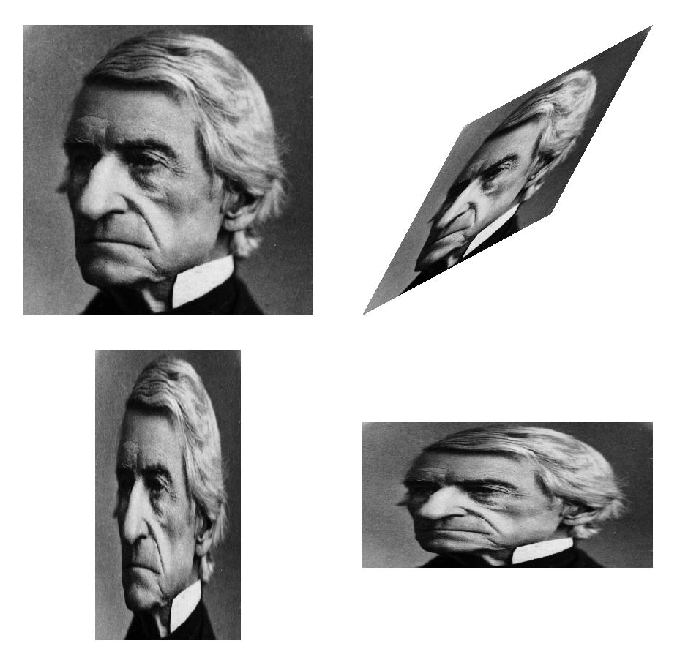
\includegraphics{fig/2-11.eps}
\caption{Изображения Уильяма Бартона Роджерса, основателя и␣первого президента MIT, нарисованные по отношению к␣тем␣же четырём рамкам, что и␣на рисунке␣\n{P2.10} (первоначальное изображение печатается с␣разрешения музея MIT).}
\label{P2.11}
\end{cntrfig}

На␣картинке \n{P2.12} показан результат работы рисовалки, называемой \c{wave4}, который строится в␣два этапа, начиная с␣\c{wave}:
\begin{code}
(define wave2 (beside wave (flip-vert wave)))
(define wave4 (below wave2 wave2))
\end{code}

Строя таким образом составные рисовалки, мы используем тот факт, что \x{замыкание|свойство замыкания языка описания картинок}рисовалки замкнуты относительно средств комбинирования нашего языка. \c{Beside} или \c{below} от двух рисовалок само является рисовалкой; следовательно, мы можем её использовать как элемент при построении ещё более сложных рисовалок. Так␣же, как при построении списковых структур с␣помощью \c{cons}, замкнутость наших данных относительно средств комбинирования служит основой способности строить сложные структуры при помощи всего лишь нескольких операций.

\begin{cntrfig}

\includegraphics{fig/2-12.eps}
\begin{code}
(define wave2                         (define wave4
  (beside wave (flip-vert wave)))       (below wave2 wave2))
\end{code}
\caption{Построение составного изображения, начиная с␣рисовалки \c{wave} с␣рисунка␣\n{P2.10}}
\label{P2.12}
\end{cntrfig}

Раз мы можем комбинировать рисовалки, нам хотелось␣бы уметь выделять типичные схемы их комбинирования. Операции над рисовалками мы реализуем как процедуры языка Scheme. Это означает, что нам в␣языке изображений не␣требуется специального механизма абстракции: поскольку средства комбинирования являются обычными процедурами Scheme, у␣нас автоматически есть право делать с␣операциями над рисовалками всё то, что мы можем делать с␣процедурами. Например, схему построения \c{wave4} мы можем абстрагировать в␣виде
\begin{code}
(define (flipped-pairs painter)\xd{\c{flipped-pairs}}
  (let ((painter2 (beside painter (flip-vert painter))))
    (below painter2 painter2)))
\end{code}
и␣определить \c{wave4} как пример применения этой схемы:
\begin{code}
(define wave4 (flipped-pairs wave))
\end{code}

Мы можем определять и␣рекурсивные операции. Вот пример, который заставляет рисовалки делиться и␣ветвиться направо, как показано на рисунках␣\n{P2.13} и␣\n{P2.14}:
\begin{code}
(define (right-split painter n) \xd{\c{right-split}}
  (if (= n 0)
      painter
      (let ((smaller (right-split painter (- n 1))))
        (beside painter (below smaller smaller)))))
\end{code}

Можно порождать сбалансированные узоры, наращивая их не␣только направо, но и␣вверх (см.␣упражнение␣\n{EX2.44} и␣рисунки␣\n{P2.13} и␣\n{P2.14}):
\begin{code}
(define (corner-split painter n)\xd{\c{corner-split}}
  (if (= n 0)
      painter
      (let ((up (up-split painter (- n 1)))
            (right (right-split painter (- n 1))))
        (let ((top-left (beside up up))
              (bottom-right (below right right))
              (corner (corner-split painter (- n 1))))
          (beside (below painter top-left)
                  (below bottom-right corner))))))
\end{code}

Соответствующим образом расположив четыре копии \c{corner-split}, мы получаем схему под названием \c{square-limit}, применение которой к␣\c{wave} и␣\c{rogers} показано на рисунке␣\n{P2.9}:
\begin{code}
(define (square-limit painter n) \xd{\c{sqare-limit}}
  (let ((quarter (corner-split painter n)))
    (let ((half (beside (flip-horiz quarter) quarter)))
      (below (flip-vert half) half))))
\end{code}

\begin{cntrfig}
\begin{tabular}{|c|c|}
\hline
                            &  \\
                            &  \c{right-split} \\
                            &  {\textit n}-1               \\
\c{identity} &                         \\ \cline{2-2}
                            & \\
                            &  \c{right-split}      \\
                            &  {\textit n}-1 \\
                            &  \\                \hline
		
\multicolumn{2}{l}{\c{right-split} \i{n}}
\end{tabular}
\hspace{1cm}
\begin{tabular}{|c|c|c|}
\hline
                &             & \\
\c{up-}        & \c{up-}    & \c{corner-split} \\
\c{split}             & \c{split}         & {\textit n}-1\\
{\textit n}-1                &  {\textit n}-1        &  \\              \hline
\multicolumn{2}{|c|}{}         &\c{right-split} \\
\multicolumn{2}{|c|}{\c{identity}} & {\textit n}-1 \\ \cline{3-3}
\multicolumn{2}{|c|}{}       & \c{right-split}\\
\multicolumn{2}{|c|}{}       & {\textit n}-1 \\
\hline
\multicolumn{3}{l}{\c{corner-split} \i{n}}
\end{tabular}
\caption{Рекурсивные планы для \c{right-split} и␣\c{corner-split}.}
\label{P2.13}
\end{cntrfig}

\begin{cntrfig}
\begin{tabular}{cc}
\multicolumn{2}{c}{
\includegraphics{fig/2-14-1.eps}} \\
\tt{(right-split wave 4)}  & \tt{(right-split rogers 4)}\\[8pt]
\multicolumn{2}{c}{
\includegraphics{fig/2-14-2.eps}} \\
\tt{(corner-split wave 4)} & \tt{(corner-split rogers 4)}
\end{tabular}

\caption{Рекурсивные операции \c{right-split} и␣\c{corner-split} в␣применении к␣рисовалкам \c{wave} и␣\c{rogers}. Комбинирование четырёх картинок \c{corner-split} даёт симметричные узоры \c{square-limit}, как показано на рисунке␣\n{P2.9}.}
\label{P2.14}
\end{cntrfig}

\begin{exercise}
Определите процедуру \x{\c{up-split}}\c{up-split}, которую использует \c{corner-split}. Она подобна \c{right-split}, но только меняет местами роли \c{below} и␣\c{beside}.
\end{exercise}
\h5{Операции высшего порядка}

\x{рисовалка|операции высшего порядка}В␣дополнение к␣абстрагированию схем комбинирования рисовалок, мы можем работать и␣на более высоком уровне, абстрагируя схемы комбинирования операций над рисовалками. А␣именно, мы можем рассматривать операции над рисовалками в␣качестве элементов, подлежащих манипуляции, и␣писать средства комбинирования этих элементов — операции, которые принимают операции над рисовалками как аргументы и␣создают новые операции.

Например, и␣\c{flipped-pairs}, и␣\c{square-limit} располагают определённым образом в␣виде квадрата четыре копии порождаемого рисовалкой изображения; они отличаются только тем, как они ориентируют эти копии. Один из способов абстрагировать такую схему комбинирования рисовалок представлен следующей процедурой, которая принимает четыре одноаргументных операции и␣порождает операцию над рисовалками, которая трансформирует данную ей рисовалку с␣помощью этих четырёх операций и␣расставляет результаты по квадрату. \c{Tl}, \c{tr}, \c{bl} и␣\c{br} — это трансформации, которые следует применить к␣верхней левой, верхней правой, нижней левой и␣нижней правой копиям, соответственно.

\begin{code}
(define (square-of-four tl tr bl br) \xd{\c{square-of-four}}
  (lambda (painter)
    (let ((top (beside (tl painter) (tr painter)))
          (bottom (beside (bl painter) (br painter))))
      (below bottom top))))
\end{code}

Тогда в␣терминах \c{square-of-four} можно определить \c{flipped-pairs} следующим образом
\f{
Мы также могли␣бы написать
\begin{code}
(define flipped-pairs\xd{\c{flipped-pairs}}
  (square-of-four identity flip-vert identity flip-vert))
\end{code}
}%f
:%%FOOTNOTE
\begin{code}
(define (flipped-pairs painter)\xd{\c{flipped-pairs}}
  (let ((combine4 (square-of-four identity flip-vert
                                  identity flip-vert)))
    (combine4 painter)))
\end{code}
а \c{square-limit} можно выразить как
\f{
\c{Rotate180} поворачивает рисовалку на 180 градусов (см.␣упражнение␣\n{EX2.50}). Вместо \c{rotate180} мы могли␣бы сказать \c{(compose flip-vert flip-horiz)}, используя процедуру \c{compose} из упражнения␣\n{EX1.42}.}

\begin{code}
(define (square-limit painter n) \xd{\c{sqare-limit}}
  (let ((combine4 (square-of-four flip-horiz identity
                                  rotate180 flip-vert)))
    (combine4 (corner-split painter n))))
\end{code}
\begin{exercise}
\c{Right-split} и␣\c{up-split} можно выразить как разновидности общей операции разделения. Определите процедуру \x{\c{split}}\c{split} с␣таким свойством, что вычисление
\begin{code}
(define right-split (split beside below))
(define up-split (split below beside))
\end{code}
порождает процедуры \c{right-split} и␣\c{up-split} с␣таким␣же поведением, как и␣определённые ранее.
\end{exercise}

\h5{Рамки}\x{рамка}

Прежде, чем мы сможем показать, как реализуются рисовалки и␣средства их комбинирования, нам нужно рассмотреть рамки. Рамку можно описать как три \x{вектор (математический)|в␣кадре из языка описания изображений}вектора — вектор исходной точки и␣два вектора краёв рамки. Вектор исходной точки $\mbox{\rm Origin}$ указывает смещение исходной точки рамки от некой абсолютной начальной точки, а␣векторы краёв $\mbox{\rm Edge}_1$ и␣$\mathop{\rm Edge}_2$ указывают смещение углов рамки от её исходной точки. Если края перпендикулярны, рамка будет прямоугольной. В␣противном случае рамка будет представлять более общий случай параллелограмма. На␣рис.␣\n{P2.15} показаны рамка и␣соответствующие ей вектора. В␣соответствии с␣принципами абстракции данных, нам пока незачем указывать, каким образом представляются рамки; нужно только сказать, что есть конструктор \c{make-frame},\x{\c{make-frame}} который принимает три вектора и␣выдаёт рамку, и␣что есть ещё три селектора, \c{origin-frame},\x{\c{origin-frame}}\x{\c{edge1-frame}}\c{edge1-frame} и␣\x{\c{edge2-frame}}\c{edge2-frame} (см.␣упражнение␣\n{EX2.47}).

\begin{cntrfig}
\input{fig/2-15.eepic}
%{\small вектор edge2 рамки\\
%вектор edge1 рамки\\
%вектор origin рамки\\
%точка (0,0) на экране дисплея}
\caption{Рамка представляется в␣виде трёх векторов — начальной точки и␣двух краёв.}
\label{P2.15}
\end{cntrfig}

Для определения изображений мы будем использовать координаты в␣\x{единичный квадрат}единичном квадрате $(0 \le x, y \le
1)$. Каждой рамке мы сопоставляем \x{рамка|отображение координат}\X{отображение координат рамки} (\E{frame coordinate map}), которое будет использоваться, чтобы сдвигать и␣масштабировать изображения так, чтобы они умещались в␣рамку. Это отображение трансформирует единичный квадрат в␣рамку, переводя вектор ${\bf v} = (x, y)$ в␣сумму векторов
$$
  \mathop{\rm Origin}(\mbox{\rm Frame})
    + x \cdot \mbox{\rm Edge}_1 (\mbox{\rm Frame})
    + y \cdot \mbox{\rm Edge}_2 (\mbox{\rm Frame})
$$

Например, (0, 0) отображается в␣исходную точку рамки, (1, 1) в␣вершину, противоположную исходной точке по диагонали, а␣(0.5, 0.5) в␣центр рамки. Мы можем создать отображение координат рамки при помощи следующей процедуры
\f{
\c{Frame-coord-map} использует векторные операции, определённые ниже в␣упражнении␣\n{EX2.46}, и␣мы предполагаем, что они реализованы для какого-нибудь представления векторов. Благодаря абстракции данных, неважно, каково это представление; нужно только, чтобы операции над векторами вели себя правильно.
}%f
:
\begin{code}
(define (frame-coord-map frame)\xd{\c{frame-coord-map}}
  (lambda (v)
    (add-vect
     (origin-frame frame)
     (add-vect (scale-vect (xcor-vect v)
                           (edge1-frame frame))
               (scale-vect (ycor-vect v)
                           (edge2-frame frame))))))
\end{code}

Заметим, что применение \c{frame-coord-map} к␣рамке даёт нам процедуру, которая, получая вектор, возвращает тоже вектор. Если вектор-аргумент находится в␣единичном квадрате, вектор-результат окажется в␣рамке. Например,
\begin{code}
((frame-coord-map a-frame) (make-vect 0 0))
\end{code}
возвращает тот␣же вектор, что и
\begin{code}
(origin-frame a-frame)
\end{code}
\begin{exercise}
Двумерный \x{вектор (математический)|операции}\x{вектор (математический)|представленный в␣виде пары}вектор ${\bf v}$, идущий от начала координат к␣точке, можно представить в␣виде пары, состоящей из $x$-координаты и␣$y$-координаты. Реализуйте абстракцию данных для векторов, написав конструктор \c{make-vect}
\x{\c{make-vect}}
и␣соответствующие селекторы \c{xcor-vect}
\x{\c{xcor-vect}}
и \c{ycor-vect}. \x{\c{ycor-vect}}
В␣терминах своих селекторов и␣конструктора реализуйте процедуры \c{add-vect}, \x{\c{add-vect}}
\c{sub-vect} и␣\c{scale-vect}, которые выполняют \x{\c{sub-vect}}
\x{\c{scale-vect}}
операции сложения, вычитания векторов и␣умножения вектора на скаляр:
$$
  \begin{array}{c}
    (x_1, y_1) + (x_2, y_2) = (x_1 + x_2, y_1 + y_2) \\
    (x_1, y_1) - (x_2, y_2) = (x_1 - x_2, y_1 - y_2) \\
    s \cdot (x, y) = (sx, sy) \\
  \end{array}
$$
\end{exercise}

\begin{exercise}
Вот два варианта конструкторов для рамок:
\begin{code}
(define (make-frame origin edge1 edge2)\xd{\c{make-frame}}
  (list origin edge1 edge2))

(define (make-frame origin edge1 edge2)
  (cons origin (cons edge1 edge2)))
\end{code}

К␣каждому из этих конструкторов добавьте соответствующие селекторы, так, чтобы получить реализацию рамок.
\end{exercise}

\h5{Рисовалки}

\x{рисовалка|представление в␣виде процедуры}Рисовалка представляется в␣виде процедуры, которая, получая в␣качестве аргумента рамку, рисует определённое изображение, отмасштабированное и␣сдвинутое так, чтобы уместиться в␣эту рамку. Это означает, что если есть рисовалка \c{p} и␣рамка \c{f}, то мы можем получить изображение, порождаемое \c{p}, в␣\c{f}, позвав \c{p} с␣\c{f} в␣качестве аргумента.

Детали того, как реализуются элементарные рисовалки, зависят от конкретных характеристик графической системы и␣типа изображения, которое надо получить. Например, пусть у␣нас будет процедура \x{\c{draw-line}}\c{draw-line}, которая рисует на экране отрезок между двумя указанными точками. Тогда мы можем создавать из списков отрезков рисовалки для изображений, состоящих из этих отрезков, вроде рисовалки \c{wave} с␣рисунка␣\n{P2.10}, таким образом
\f{
Процедура \c{segments->painter} использует представление отрезков прямых, описанное ниже в␣упражнении␣\n{EX2.48}. Кроме того, она использует процедуру \c{for-each}, описанную в␣упражнении␣\n{EX2.23}.
}%f
:
\begin{code}
(define (segments->painter segment-list)\xd{\c{segments->painter}}
  (lambda (frame)
    (for-each
     (lambda (segment)
       (draw-line
        ((frame-coord-map frame) (start-segment segment))
        ((frame-coord-map frame) (end-segment segment))))
     segment-list)))
\end{code}

Отрезки даются в␣координатах по отношению к␣единичному квадрату. Для каждого сегмента в␣списке рисовалка преобразует концы отрезка с␣помощью отображения координат рамки и␣рисует отрезок между точками с␣преобразованными координатами.

Представление рисовалок в␣виде процедур воздвигает в␣языке построения изображений мощный барьер абстракции. Мы можем создавать и␣смешивать множество типов элементарных рисовалок, в␣зависимости от имеющихся возможностей графики. Детали их реализации несущественны. Любая процедура, если она принимает в␣качестве аргумента рамку и␣рисует в␣ней что-нибудь должным образом отмасштабированное, может служить рисовалкой
\f{
Например, рисовалка \c{rogers} с␣рисунка␣\n{P2.11} была получена из полутонового чёрно-белого изображения. Для каждой точки в␣указанной рамке рисовалка \c{rogers} определяет точку исходного изображения, которая в␣неё отображается, и␣соответствующим образом её окрашивает. Разрешая себе иметь различные типы рисовалок, мы пользуемся идеей абстрактных данных, описанной в␣\r{what-is-meant-by-data}{разделе␣\n}, где мы говорили, что представление рациональных чисел может быть каким угодно, пока соблюдается соответствующее условие. Здесь мы используем то, что рисовалку можно реализовать как угодно, лишь␣бы она что-то изображала в␣указанной рамке. В␣\r{what-is-meant-by-data}{разделе␣\n} показывается и␣то, как реализовать пары в␣виде процедур. Рисовалки — это наш второй пример процедурного представления данных.
}\fa.
\begin{exercise}
Направленный отрезок на плоскости можно представить в␣виде пары векторов:\x{отрезок|представление в␣виде пары векторов} вектор от начала координат до начала отрезка и␣вектор от начала координат до конца отрезка. Используйте своё представление векторов из упражнения␣\n{EX2.46} и␣определите представление отрезков с␣конструктором \c{make-segment}
\x{\c{make-segment}}
и␣селекторами \c{start-segment}
\x{\c{start-segment}}
и \c{end-segment}. \x{\c{end-segment}}
\end{exercise}

\begin{exercise}
С␣помощью \c{segments->painter} определите следующие элементарные рисовалки:

\begin{plainenum}
\item Рисовалку, которая обводит указанную рамку.

\item Рисовалку, которая рисует «Х», соединяя противоположные концы рамки.

\item Рисовалку, которая рисует ромб, соединяя между собой середины сторон рамки.

\item Рисовалку \c{wave}.
\end{plainenum}
\end{exercise}

\h5{Преобразование и␣комбинирование рисовалок}

\x{рисовалка|преобразование и␣комбинирование}Операции над рисовалками (\c{flip-vert} или \c{beside}, например) создают новые рисовалки, которые вызывает исходные рисовалки по отношению к␣рамкам, производным от рамок-аргументов. Таким образом, скажем, \c{flip-vert} не␣требуется знать, как работает рисовалка, чтобы перевернуть её — ей нужно только уметь перевернуть рамку вверх ногами: перевёрнутая рисовалка просто использует исходную, но в␣обращённой рамке.

Операции над рисовалками основываются на процедуре \c{transform-painter}, которая в␣качестве аргументов берёт рисовалку и␣информацию о␣том, как преобразовать рамку, а␣возвращает новую рисовалку. Когда преобразованная рисовалка вызывается по отношению к␣какой-либо рамке, она преобразует рамку и␣вызывает исходную рисовалку по отношению к␣ней. Аргументами \c{transform-painter} служат точки (представленные в␣виде векторов), указывающие углы новой рамки: будучи отображённой на рамку, первая точка указывает исходную точку новой рамки, а␣две других — концы краевых векторов. Таким образом, аргументы, лежащие в␣пределах единичного квадрата, определяют рамку, которая содержится внутри исходной рамки.

\begin{code}
(define (transform-painter painter origin corner1 corner2)\xd{\c{transform-painter}}
  (lambda (frame)
    (let ((m (frame-coord-map frame)))
      (let ((new-origin (m origin)))
        (painter
         (make-frame new-origin
                     (sub-vect (m corner1) new-origin)
                     (sub-vect (m corner2) new-origin)))))))
\end{code}

Вот как перевернуть изображение в␣рамке вертикально:
\begin{code}
(define (flip-vert painter)\xd{\c{flip-vert}}
  (transform-painter painter
                     (make-vect 0.0 1.0)  \e{; новая исходная точка}
                     (make-vect 1.0 1.0)  \e{; новый конец \c{edge1}}
                     (make-vect 0.0 0.0)))\e{; новый конец \c{edge2}}
\end{code}

При помощи \c{transform-painter} нам нетрудно будет определять новые трансформации. Например, можно определить рисовалку, которая рисует уменьшенную копию исходного изображения в␣верхней правой четверти рамки:
\begin{code}
(define (shrink-to-upper-right painter) \xd{\c{shrink-to-upper-right}}
  (transform-painter painter
                     (make-vect 0.5 0.5)
                     (make-vect 1.0 0.5)
                     (make-vect 0.5 1.0)))
\end{code}

Вот трансформация, которая поворачивает изображение на 90 градусов против часовой стрелки
\f{
\c{Rotate90} представляет собой чистый поворот только для квадратных рамок, поскольку она ещё растягивает и␣сплющивает изображение так, чтобы оно уместилось в␣повёрнутой рамке.
}%f
:
\begin{code}
(define (rotate90 painter) \xd{\c{rotate90}}
  (transform-painter painter
                     (make-vect 1.0 0.0)
                     (make-vect 1.0 1.0)
                     (make-vect 0.0 0.0)))
\end{code}

А␣эта сжимает изображение по направлению к␣центру рамки
\f{
Ромбовидные изображения на рисунках␣\n{P2.10} и␣\n{P2.11} были получены с␣помощью \c{squash-inwards}, применённой к␣\c{wave} и␣\c{rogers}.
}%f
:
\begin{code}
(define (squash-inwards painter) \xd{\c{squash-inwards}}
  (transform-painter painter
                     (make-vect 0.0 0.0)
                     (make-vect 0.65 0.35)
                     (make-vect 0.35 0.65)))
\end{code}

Преобразования рамок являются также основой для определения средств комбинирования двух или более рисовалок. Например, процедура \c{beside} берёт две рисовалки, трансформирует их так, чтобы они работали соответственно в␣левой и␣правой половинах рамки-аргумента, и␣создаёт новую составную рисовалку. Когда составной рисовалке передаётся рамка, она вызывает первую из преобразованных рисовалок над левой половиной рамки, а␣вторую над правой половиной:
\begin{code}
(define (beside painter1 painter2)\xd{\c{beside}}
  (let ((split-point (make-vect 0.5 0.0)))
    (let ((paint-left
           (transform-painter painter1
                              (make-vect 0.0 0.0)
                              split-point
                              (make-vect 0.0 1.0)))
          (paint-right
           (transform-painter painter2
                              split-point
                              (make-vect 1.0 0.0)
                              (make-vect 0.5 1.0))))
      (lambda (frame)
        (paint-left frame)
        (paint-right frame)))))
\end{code}

Обратите внимание, как абстракция данных, и␣особенно представление рисовалок в␣виде процедур, облегчает реализацию \c{beside}. Процедуре \c{beside} не␣требуется ничего знать о␣деталях рисовалок-компонент, кроме того, что каждая из них что-то изобразит в␣указанной ей рамке.
\begin{exercise}
Определите преобразование \c{flip-horiz}, \x{\c{flip-horiz}}
которое обращает изображение вокруг горизонтальной оси, а␣также преобразования, которые вращают рисовалки против часовой стрелки на 180 и␣270 градусов.
\end{exercise}

\begin{exercise}
Определите для рисовалок операцию \c{below}. \x{\c{below}}
\c{Below} принимает в␣качестве аргументов две рисовалки. Когда получившейся рисовалке передаётся рамка, она рисует в␣нижней её половине при помощи первой рисовалки, а␣в␣верхней при помощи второй. Определите \c{below} двумя способами — один раз аналогично процедуре \c{beside}, как она приведена выше, а␣второй раз через \c{beside} и␣операции вращения (см.␣упражнение␣\n{EX2.50}).
\end{exercise}

\h5{Уровни языка помогают устойчивому проектированию}

Язык построения изображений использует некоторые из важнейших введённых нами идей, относящихся к␣абстракции процедур и␣данных. Базовая абстракция данных, рисовалки, реализуется при помощи процедурного представления, и␣благодаря этому наш язык может работать с␣различными графическими системами единым образом. Средства комбинирования обладают свойством замыкания, и␣это позволяет нам легко возводить сложные построения. Наконец, все средства абстракции процедур доступны нам для того, чтобы абстрагировать средства комбинирования рисовалок.

Нам удалось бросить взгляд и␣ещё на одну существеннейшую идею касательно проектирования языков и␣программ. Это подход \x{уровневое проектирование}\e{уровневого проектирования} (\E{stratified design}), представление, что сложной системе нужно придавать структуру при помощи последовательности уровней, которая описывается последовательностью языков. Каждый из уровней строится путём комбинации частей, которые на этом уровне рассматриваются как элементарные, и␣части, которые строятся на каждом уровне, работают как элементарные на следующем уровне. Язык, который используется на каждом уровне такого проекта, включает примитивы, средства комбинирования и␣абстракции, соответствующие этому уровню подробности.

Уровневое проектирование пронизывает всю технику построения сложных систем. Например, при проектировании компьютеров резисторы и␣транзисторы сочетаются (и␣описываются при помощи языка аналоговых схем), и␣из них строятся и-, или- элементы и␣им подобные, служащие основой языка цифровых схем
\f{
Один из таких языков описывается в␣\r{a-simulator-for-digital-circuits}{разделе␣\n}.
}%f
\fa. Из␣этих элементов строятся процессоры, шины и␣системы памяти, которые в␣свою очередь служат элементами в␣построении компьютеров при помощи языков, подходящих для описания компьютерной архитектуры. Компьютеры, сочетаясь, дают распределённые системы, которые описываются при помощи языков описания сетевых взаимодействий, и␣так далее.

Как миниатюрный пример уровневого подхода, наш язык описания изображений использует элементарные объекты (элементарные рисовалки), создаваемые при помощи языка, в␣котором описываются точки и␣линии и␣создаются списки отрезков для рисовалки \c{segments->painter} либо градации серого цвета в␣рисовалке вроде \c{rogers}. Большей частью наше описание языка картинок было сосредоточено на комбинировании этих примитивов с␣помощью геометрических комбинаторов вроде \c{beside} и␣\c{below}. Работали мы и␣на более высоком уровне, где \c{beside} и␣\c{below} рассматривались как примитивы, манипулируемые языком, операции которого, такие как \c{square-of-four}, фиксируют стандартные схемы сочетания геометрических комбинаторов.

Уровневое проектирование помогает придать программам \x{устойчивость программы}\e{устойчивость} (\E{robustness}), то есть повышает вероятность, что небольшое изменение в␣спецификации потребует относительно малых изменений в␣программе. Например, предположим, что нам нужно изменить картинку, основанную на рисовалке \c{wave}, которая показана на рисунке␣\n{P2.9}. Мы можем работать на самом низком уровне, изменяя конкретный вид элемента \c{wave}; можем работать на промежуточном уровне и␣менять то, как \c{corner-split} воспроизводит \c{wave}; можем на самом высоком уровне изменять то, как \c{square-limit} расставляет четыре копии по углам. В␣общем, каждый уровень такого проекта даёт свой словарь для описания характеристик системы и␣свой тип возможных изменений.
\begin{exercise}
Измените предел квадрата рисовалки \c{wave}, показанный на рисунке␣\n{P2.9}, работая на каждом из вышеописанных уровней. А␣именно:

\begin{plainenum}
\item Добавьте новые отрезки к␣элементарной рисовалке \c{wave} из упражнения␣\n{EX2.49} (например, изобразив улыбку).

\item Измените шаблон, который порождает \c{corner-split} (например, используя только одну копию образов \c{up-split} и␣\c{right-split} вместо двух).

\item Измените версию \c{square-limit}, использующую \c{square-of-four}, так, чтобы углы компоновались как-нибудь по-другому. (Например, можно сделать так, чтобы большой мистер Роджерс выглядывал из каждого угла квадрата.)
\end{plainenum}
\end{exercise}

\l{symbolic-data}
\h2{Символьные данные}

\x{символ(ы)}Все составные объекты данных, которые мы до сих пор использовали, состояли, в␣конечном счёте, из чисел. В␣этом разделе мы расширяем возможности представления нашего языка, разрешая использовать в␣качестве данных \x{данные|символьные}произвольные символы.

\l{quotation}
\h3{Кавычки}

\x{кавычки}Раз теперь нам можно формировать составные данные, используя символы, мы можем пользоваться списками вроде
\begin{code}
(a b c d)
(23 45 17)
((Norah 12) (Molly 9) (Anna 7) (Lauren 6) (Charlotte 3))
\end{code}
\x{Сассман, Джули Эстер Мазель, племянницы}
Списки, содержащие символы, могут выглядеть в␣точности как выражения нашего языка:
\begin{code}
(* (+ 23 45) (+ x 9))

(define (fact n) (if (= n 1) 1 (* n (fact (- n 1)))))
\end{code}

Чтобы работать с␣символами, нам в␣языке нужен новый элемент: способность \x{кавычка}\e{закавычить} (\E{quote}) объект данных. Допустим, нам хочется построить список \c{(a b)}. Этого нельзя добиться через \c{(list a b)}, поскольку это выражение строит список из \e{значений} символов \c{a} и␣\c{b}, а␣не␣из них самих. Этот вопрос хорошо изучен по отношению к␣естественным языкам, где слова и␣предложения могут рассматриваться либо как семантические единицы, либо как строки символов (синтаксические единицы). \x{естественный язык|кавычки}\s{язык}\x{кавычки|в␣естественном языке}В␣естественных языках обычно используют кавычки, чтобы обозначить, что слово или предложение нужно рассматривать буквально как строку символов. Например, первая буква «Джона» — разумеется,␣«Д». Если мы говорим кому-то «скажите, как вас зовут», мы ожидаем услышать имя этого человека. Если␣же мы говорим кому-то «скажите
„как вас зовут“», то мы ожидаем услышать слова «как вас зовут». Заметьте, как, для того, чтобы описать, что должен сказать кто-то другой, нам пришлось использовать кавычки
\f{
Когда мы разрешаем в␣языке кавычки, это разрушает нашу способность говорить о␣языке в␣простых терминах, поскольку становится неверным, что равнозначные выражения можно подставлять друг вместо друга. Например, три есть два плюс один, но слово «три» не␣есть слова «два плюс один». Кавычки являются мощным инструментом, поскольку они дают нам способ строить выражения, которые работают с␣другими выражениями (как мы убедимся в␣\r{metalinguistic-abstraction}{главе␣\n}, когда станем писать интерпретатор). Однако как только мы разрешаем в␣языке выражения, которые говорят о␣других выражениях того␣же языка, становится очень сложно соблюдать в␣каком-либо виде принцип «равное можно заменить равным». Например, если мы знаем, что утренняя и␣вечерняя звезда — одно и␣то␣же, то из утверждения \x{Венера}\s{утренняя звезда}\s{вечерняя звезда}«вечерняя звезда — это Венера» мы можем заключить, что «утренняя звезда — это Венера». Однако если нам дано, что «Джон знает, что вечерняя звезда — это Венера», мы не␣можем заключить, что «Джон знает, что утренняя звезда — это Венера».
}\fa.

Чтобы обозначать списки и␣символы, с␣которыми нужно обращаться как с␣\x{кавычки|с␣объектами данных Лиспа}объектами данных, а␣не␣как с␣выражениями, которые нужно вычислить, мы можем следовать тому␣же обычаю. Однако наш формат кавычек отличается от принятого в␣естественных языках тем, что мы ставим знак кавычки (по␣традиции, это символ одинарной кавычки \c{'}) только в␣начале того объекта, который надо закавычить. В␣Scheme это сходит нам с␣рук, поскольку для разделения объектов мы полагаемся на пробелы и␣скобки. Таким образом, значением одинарной кавычки является требование закавычить следующий объект
\f{
\x{кавычки|одинарная vs.␣двойные}\x{строка|печатание}\x{кавычки|со строкой символов}Одинарная кавычка отличается от двойной, которую мы использовали для обозначения строк, выводимых на печать. В␣то время как \x{\c{'} (одинарная кавычка)}одинарную кавычку можно использовать для обозначения списков символов, \x{\c{"} (двойная кавычка)}двойная кавычка используется только со строками, состоящими из печатных знаков. Единственное, для чего такие строки используются в␣нашей книге — это печать.
}\fa.

\x{символ(ы)|кавычки}Теперь мы можем отличать символы от их значений:
\begin{code}
(define a 1)

(define b 2)

(list a b)
\resp{(1 2)}

(list 'a 'b)
\resp{(a b)}

(list 'a b)
\resp{(a 2)}
\end{code}

\x{список|кавычки}Кроме того, кавычки позволяют нам вводить составные объекты, используя обычное представление для печати списков:
\f{
Строго говоря, то, как мы используем кавычку, нарушает общее правило, что все сложные выражения нашего языка должны отмечаться скобками и␣выглядеть как списки. Мы можем восстановить эту закономерность, введя особую форму \x{\c{quote} (особая форма)}\x{особые формы|\c{quote}}\c{quote}, которая служит тем␣же целям, что и␣кавычка. Таким образом, мы можем печатать \c{(quote a)} вместо \c{'a} и␣\c{(quote (a b c))} вместо \c{'(a b c)}. Именно так и␣работает интерпретатор. Знак кавычки — это просто сокращение, означающее, что следующее выражение нужно завернуть в␣форму \c{quote} и␣получить \c{(quote \prm{выражение})}. Это важно потому, что таким образом соблюдается принцип, что с␣любым выражением, которое видит интерпретатор, можно обращаться как с␣объектом данных. Например, можно получить выражение \c{(car '(a b c))}, и␣это будет то␣же самое, что и␣\c{(car (quote (a b c)))}, вычислив \c{(list 'car (list 'quote '(a b c)))}.
}\fa.

\begin{code}
(car '(a b c))
\resp{a}

(cdr '(a b c))
\resp{(b c)}
\end{code}

Действуя в␣том␣же духе, пустой список мы можем получить, вычисляя \c{'()}, и␣таким образом избавиться от переменной \c{nil}. \x{\c{nil}|избавление от}

Ещё один примитив, который используется при работе с␣символами — это \c{eq?}, \xd{\c{eq?} (элементарная процедура)}
\x{элементарные процедуры|\c{eq?}}
\x{символ(ы)|равенство} который берёт в␣качестве аргументов два символа и␣проверяет, совпадают␣ли они
\f{
\x{равенство|символов}Можно считать, что два символа «совпадают», если они состоят из одних и␣тех␣же печатных знаков в␣одинаковом порядке. Такое определение обходит важный вопрос, который мы пока не␣готовы обсуждать: значение «одинаковости» в␣языке программирования. К␣нему мы вернёмся в␣\r{modularity-objects-and-state}{главе␣\n}
\r{the-costs-of-introducing-assignment}{(раздел␣\n)}.
}\fa.

С␣помощью \c{eq?} можно реализовать полезную процедуру, называемую \c{memq}. Она принимает два аргумента, символ и␣список. Если символ не␣содержится в␣списке (то␣есть, не␣равен в␣смысле \c{eq?} ни␣одному из элементов списка), то \c{memq} возвращает ложь. В␣противном случае она возвращает подсписок списка, начиная с␣первого вхождения символа:
\begin{code}
(define (memq item x)\xd{\c{memq}}
  (cond ((null? x) false)
        ((eq? item (car x)) x)
        (else (memq item (cdr x)))))
\end{code}

Например, значение
\begin{code}
(memq 'apple '(pear banana prune))
\end{code}
есть ложь, в␣то время как значение
\begin{code}
(memq 'apple '(x (apple sauce) y apple pear))
\end{code}
есть \c{(apple pear)}.
\begin{exercise}
Что напечатает интерпретатор в␣ответ на каждое из следующих выражений?

\begin{code}
(list 'a 'b 'c)

(list (list 'george))

(cdr '((x1 x2) (y1 y2)))

(cadr '((x1 x2) (y1 y2)))

(pair? (car '(a short list)))

(memq 'red '((red shoes) (blue socks)))

(memq 'red '(red shoes blue socks))
\end{code}
\end{exercise}

\begin{exercise}
\x{список|равенство} \x{равенство|списков}Предикат \c{equal?}\x{\c{equal?}}
для двух списков возвращает истину, если они содержат одни и␣те␣же элементы в␣одинаковом порядке. Например,
\begin{code}
(equal? '(this is a list) '(this is a list))
\end{code}
истинно, но
\begin{code}
(equal? '(this is a list) '(this (is a) list))
\end{code}
ложно. Более точно, можно определить \c{equal?} рекурсивно в␣терминах базового равенства символов \c{eq?}, сказав, что \c{a} равно \c{b}, если оба они символы и␣для них выполняется \c{eq?} либо оба они списки и␣при этом верно, что \c{(car a)} равняется в␣смысле \c{equal?}
\c{(car b)}, а␣\c{(cdr a)} равняется в␣смысле \c{equal?} \c{(cdr b)}. Пользуясь этой идеей, напишите \c{equal?} в␣виде процедуры
\f{
На␣практике программисты используют \c{equal?} для\x{равенство|чисел}\x{числа|равенство} сравнения не␣только символов, но и␣чисел. Числа не␣считаются символами. Вопрос о␣том, выполняется ли \c{eq?} для двух чисел, которые равны между собой (в␣смысле \c{=}), очень сильно зависит от конкретной реализации. Более правильное определение \c{equal?} (например, то, которое входит в␣Scheme как элементарная процедура) должно содержать условие, что если и␣\c{a}, и␣\c{b} являются числами, то \c{equal?} для них выполняется тогда, когда они численно равны.
}\fa.
\end{exercise}

\begin{exercise}
Ева Лу Атор вводит при работе с␣интерпретатором выражение
\begin{code}
(car ''abracadabra)
\end{code}

К␣её удивлению, интерпретатор печатает \c{quote}. Объясните.
\end{exercise}

\l{example-symbolic-differentiation}
\h3{Пример: символьное дифференцирование}

\x{дифференцирование|символьное}\x{символьное дифференцирование}\x{алгебраическое выражение|дифференцирование}Как иллюстрацию к␣понятию символьной обработки, а␣также как дополнительный пример абстракции данных, рассмотрим построение процедуры, которая производит символьное дифференцирование алгебраических выражений. Нам хотелось␣бы, чтобы эта процедура принимала в␣качестве аргументов алгебраическое выражение и␣переменную, и␣чтобы она возвращала производную выражения по отношению к␣этой переменной. Например, если аргументами к␣процедуре служат $ax^2 + bx +
c$ и␣$x$, процедура должна возвращать $2ax +
b$. Символьное дифференцирование имеет для Лиспа особое историческое значение. Оно было одним из побудительных примеров при разработке компьютерного языка для обработки символов. Более того, оно послужило началом линии исследований, приведшей к␣разработке мощных систем для символической математической работы, которые сейчас всё больше используют прикладные математики и␣физики.

При разработке программы для символьного дифференцирования мы будем следовать той␣же самой стратегии абстракции данных, согласно которой мы действовали при разработке системы рациональных чисел в␣\r{exmp-arith-oper-for-rat-numbers}{разделе␣\n}. А␣именно, сначала мы разработаем алгоритм дифференцирования, который работает с␣абстрактными объектами, такими как «суммы», «произведения» и␣«переменные», не␣обращая внимания на то, как они должны быть представлены. Только после этого мы обратимся к␣задаче представления.

\h5{Программа дифференцирования с␣абстрактными данными}

Чтобы упростить задачу, мы рассмотрим простую программу \x{дифференцирование|правила}символьного дифференцирования, которая работает с␣выражениями, построенными только при помощи операций сложения и␣умножения с␣двумя аргументами. Дифференцировать любое такое выражение можно, применяя следующие правила редукции:
$$
   \frac{dc}{dx} = 0\ \mbox{\rm для константы либо переменной, отличной от␣$x$}
$$

$$
  \frac{dx}{dx} = 1
$$

$$
  \frac{d(u+v)}{dx} = \frac{du}{dx} + \frac{dv}{dx}
$$

$$
  \frac{d(uv)}{dx} = u (\frac{dv}{dx}) + v (\frac{du}{dx})
$$

Заметим, что два последних правила по сути своей рекурсивны. То␣есть, чтобы получить производную суммы, нам сначала нужно получить производные слагаемых и␣их сложить. Каждое из них в␣свою очередь может быть выражением, которое требуется разложить на составляющие. Разбивая их на всё более мелкие части, мы в␣конце концов дойдём до стадии, когда все части являются либо константами, либо переменными, и␣их производные будут равны либо 0, либо␣1.

Чтобы воплотить эти правила в␣виде процедуры, мы позволим себе немного \x{мечтать не␣вредно}помечтать, подобно тому, как мы делали при реализации рациональных чисел. Если␣бы у␣нас был способ представления алгебраических выражений, мы могли␣бы проверить, является␣ли выражение суммой, произведением, константой или переменной. Можно было␣бы извлекать части выражений. Например, для суммы мы хотели␣бы уметь получать первое и␣второе слагаемое. Ещё нам нужно уметь составлять выражения из частей. Давайте предположим, что у␣нас уже есть процедуры, которые реализуют следующие селекторы, конструкторы и␣предикаты:

\begin{plainlist}
\item {\bf \c{(variable? e)}} \x{\c{variable?}}
Является␣ли \c{e} переменной?
\item {\bf \c{(same-variable? v1 v2)}} \x{\c{same-variable?}}
Являются␣ли \c{v1} и␣\c{v2} одной и␣той␣же переменной?
\item {\bf \c{(sum? e)}} \x{\c{sum?}}
Является␣ли \c{e} суммой?
\item {\bf \c{(addend e)}} \x{\c{addend}}
Первое слагаемое суммы \c{e}.
\item {\bf \c{(augend e)}} \x{\c{augend}}
Второе слагаемое суммы \c{e}.
\item {\bf \c{(make-sum a1 a2)}} \x{\c{make-sum}}
Строит сумму \c{a1} и␣\c{a2}.
\item {\bf \c{(product? e)}} \x{\c{product?}}
Является␣ли \c{e} произведением?
\item {\bf \c{(multiplier e)}} Первый множитель произведения \c{e}.
\item {\bf \c{(multiplicand e)}} Второй множитель произведения \c{e}.
\item {\bf \c{(make-product m1 m2)}} \x{\c{make-product}}
Строит произведение \c{m1} и␣\c{m2}.
\end{plainlist}

При помощи этих процедур и␣элементарного предиката \c{number?}, \xd{\c{number?} (элементарная процедура)}
\x{элементарные процедуры|\c{number}}
который распознаёт числа, мы можем выразить правила дифференцирования в␣виде следующей процедуры:
\begin{code}
(define (deriv exp var)\xd{\c{deriv} (символическая)}
  (cond ((number? exp) 0)
        ((variable? exp)
         (if (same-variable? exp var) 1 0))
        ((sum? exp)
         (make-sum (deriv (addend exp) var)
                   (deriv (augend exp) var)))
        ((product? exp)
         (make-sum
           (make-product (multiplier exp)
                         (deriv (multiplicand exp) var))
           (make-product (deriv (multiplier exp) var)
                         (multiplicand exp))))
        (else
         (error "неизвестный тип выражения -- DERIV" exp))))
\end{code}

Процедура \c{deriv} заключает в␣себе весь алгоритм дифференцирования. Поскольку она выражена в␣терминах абстрактных данных, она будет работать, как␣бы мы ни␣представили алгебраические выражения, если только у␣нас будут соответствующие селекторы и␣конструкторы. Именно этим вопросом нам и␣нужно теперь заняться.

\h5{Представление алгебраических выражений}

Можно представить себе множество способов представления алгебраических выражений с␣помощью списковых структур. Например, можно использовать списки символов, которые отражали␣бы обычную алгебраическую нотацию, так что $ax + b$ представлялось␣бы как список \c{(a * x + b)}. Однако естественней всего использовать ту␣же скобочную префиксную запись, с␣помощью которой в␣Лиспе представляются комбинации; то есть представлять $ax +
b$ в␣виде \c{(+ (* a x) b)}. Тогда наше представление данных для задачи дифференцирования будет следующим: \x{алгебраическое выражение|представление}

\begin{plainlist}
\item Переменные — это символы. Они распознаются элементарным предикатом \c{symbol?}: \x{элементарные процедуры|\c{symbol?}} \xd{\c{symbol?} (элементарная процедура)}

\begin{code}
(define (variable? x) (symbol? x))
\end{code}

\item Две переменные одинаковы, если для представляющих их символов выполняется \c{eq?}:
\begin{code}
(define (same-variable? v1 v2) \xd{\c{same-variable?}}
  (and (variable? v1) (variable? v2) (eq? v1 v2)))
\end{code}

\item Суммы и␣произведения конструируются как списки:
\begin{code}
(define (make-sum a1 a2) (list '+ a1 a2))\xd{\c{make-sum}}

(define (make-product m1 m2) (list '* m1 m2))\xd{\c{make-product}}
\end{code}

\item Сумма — это список, первый элемент которого символ \c{+}:
\begin{code}
(define (sum? x) \xd{\c{sum?}}
  (and (pair? x) (eq? (car x) '+)))
\end{code}

\item Первое слагаемое — это второй элемент списка, представляющего сумму:
\begin{code}
(define (addend s) (cadr s))\xd{\c{addend}}
\end{code}

\item Второе слагаемое — это третий элемент списка, представляющего сумму:
\begin{code}
(define (augend s) (caddr s))\xd{\c{augend}}
\end{code}

\item Произведение — это список, первый элемент которого символ \c{*}:
\begin{code}
(define (product? x) \xd{\c{product?}}
  (and (pair? x) (eq? (car x) '*)))
\end{code}

\item Первый множитель — это второй элемент списка, представляющего произведение:
\begin{code}
(define (multiplier p) (cadr p))\xd{\c{multiplier}|селектор}
\end{code}

\item Второй множитель — это третий элемент списка, представляющего произведение:
\begin{code}
(define (multiplicand p) (caddr p))\xd{\c{multiplicand}}
\end{code}
\end{plainlist}

Таким образом, нам осталось только соединить это представление с␣алгоритмом, заключённым в␣процедуре \c{deriv}, и␣мы получаем работающую программу символьного дифференцирования. Посмотрим на некоторые примеры её поведения:
\begin{code}
(deriv '(+ x 3) 'x)
\resp{(+ 1 0)}

(deriv '(* x y) 'x)
\resp{(+ (* x 0) (* 1 y))}

(deriv '(* (* x y) (+ x 3)) 'x)
\resp{(+ (* (* x y) (+ 1 0))}
   \resp{(* (+ (* x 0) (* 1 y))}
      \resp{(+ x 3)))}
\end{code}

Ответы, которые выдаёт программа, правильны; однако их нужно упрощать. Верно, что
$$
  \frac{d(xy)}{dx} = x \cdot 0 + 1 \cdot y
$$
но нам хотелось␣бы, чтобы программа знала, что $x \cdot 0 =
0$, $1 \cdot y = y$, а␣$0 + y =
y$. Ответом на второй пример должно быть просто␣$y$. Как видно из третьего примера, при усложнении выражений упрощение превращается в␣серьёзную проблему.

\x{упрощение алгебраических выражений}\x{алгебраическое выражение|упрощение}
Наши теперешние затруднения очень похожи на те, с␣которыми мы столкнулись при реализации рациональных чисел: мы не␣привели ответы к␣простейшей форме. Чтобы произвести приведение рациональных чисел, нам потребовалось изменить только конструкторы и␣селекторы в␣нашей реализации. Здесь мы можем применить подобную␣же стратегию. Процедуру \c{deriv} мы не␣будем изменять вовсе. Вместо этого мы изменим \c{make-sum} так, что если оба слагаемых являются числами, она их сложит и␣вернёт их сумму. Кроме того, если одно из слагаемых равно 0, то \c{make-sum} вернёт другое.

\begin{code}
(define (make-sum a1 a2)
  (cond ((=number? a1 0) a2)
        ((=number? a2 0) a1)
        ((and (number? a1) (number? a2)) (+ a1 a2))
        (else (list '+ a1 a2))))
\end{code}

Здесь используется процедура \c{=number?}, которая проверяет, не␣равно␣ли выражение определённому числу:
\begin{code}
(define (=number? exp num)\xd{\c{=number?}}
  (and (number? exp) (= exp num)))
\end{code}

Подобным␣же образом мы изменим и␣\c{make-product}, так. чтобы встроить в␣него правила, что нечто, умноженное на␣0, есть 0, а␣умноженное на␣1 равно самому себе:
\begin{code}
(define (make-product m1 m2)
  (cond ((or (=number? m1 0) (=number? m2 0)) 0)
        ((=number? m1 1) m2)
        ((=number? m2 1) m1)
        ((and (number? m1) (number? m2)) (* m1 m2))
        (else (list '* m1 m2))))
\end{code}

Вот как эта версия работает на наших трёх примерах:
\begin{code}
(deriv '(+ x 3) 'x)
\resp{1}

(deriv '(* x y) 'x)
\resp{y}

(deriv '(* (* x y) (+ x 3)) 'x)
\resp{(+ (* x y) (* y (+ x 3)))}
\end{code}

Хотя это заметное улучшение, третий пример показывает, что нужно многое ещё сделать, прежде чем мы получим программу, приводящую выражения к␣форме, которую мы согласимся считать «простейшей». Задача алгебраического упрощения сложна, среди прочего, ещё и␣потому, что форма, которая является простейшей для одних целей, может таковой не␣являться для других.
\begin{exercise}
\x{дифференцирование|правила} Покажите, как расширить простейшую программу дифференцирования так, чтобы она воспринимала больше разных типов выражений. Например, реализуйте правило взятия производной
$$
  \frac{d(u^n)}{dx} = n u^{n-1} (\frac{du}{dx})
$$
добавив ещё одну проверку к␣программе \c{deriv} и␣определив соответствующие процедуры \c{exponentiation?}, \c{base}, \c{exponent} и␣\c{make-exponentiation} (обозначать возведение в␣степень можно символом \c{**}). Встройте правила, что любое выражение, возведённое в␣степень 0, даёт 1, а␣возведённое в␣степень 1 равно самому себе.
\end{exercise}

\begin{exercise}
Расширьте программу дифференцирования так, чтобы она работала с␣суммами и␣произведениями любого (больше двух) количества термов. Тогда последний из приведённых выше примеров мог␣бы быть записан как
\begin{code}
(deriv '(* x y (+ x 3)) 'x)
\end{code}

Попытайтесь сделать это, изменяя только представление сумм и␣произведений, не␣трогая процедуру \c{deriv}. Тогда, например, процедура \c{addend} будет возвращать первое слагаемое суммы, а␣\c{augend} сумму остальных.
\end{exercise}

\begin{exercise}
\x{инфиксная нотация vs.␣префиксная нотация} \x{префиксная нотация|vs.␣инфиксная нотация}Предположим, что нам захотелось изменить программу дифференцирования так, чтобы она работала с␣обычной математической нотацией, где \c{+} и␣\c{*} не␣префиксные, а␣инфиксные операции. Поскольку программа взятия производных определена в␣терминах абстрактных данных, мы можем изменять представление выражений, с␣которыми она работает, меняя только предикаты, селекторы и␣конструкторы, определяющие представление алгебраических выражений, с␣которыми должен работать дифференциатор.

\begin{plainenum}
\item Покажите, как это сделать так, чтобы брать производные от выражений, представленных в␣инфиксной форме, например \c{(x + (3 * (x + (y + 2))))}. Для упрощения задачи предположите, что \c{+} и␣\c{*} всегда принимают по два аргумента, и␣что в␣выражении расставлены все скобки.

\item Задача становится существенно сложней, если мы разрешаем стандартную алгебраическую нотацию, например \c{(x + 3 * (x + y + 2))}, которая опускает ненужные скобки и␣предполагает, что умножение выполняется раньше, чем сложение. Можете␣ли вы разработать соответствующие предикаты, селекторы и␣конструкторы для этой нотации так, чтобы наша программа взятия производных продолжала работать?
\end{plainenum}
\end{exercise}

\l{example-representing-sets}
\h3{Пример: представление множеств}

\x{множество}В␣предыдущих примерах мы построили представления для двух типов составных объектов: для рациональных чисел и␣для алгебраических выражений. В␣одном из этих примеров перед нами стоял выбор, упрощать␣ли выражение при его конструировании или при обращении; в␣остальном␣же выбор представления наших структур через списки был простым делом. Когда мы обращаемся к␣представлению множеств, выбор представления не␣так очевиден. Здесь существует несколько возможных представлений, и␣они значительно отличаются друг от друга в␣нескольких аспектах.

Говоря неформально, множество есть просто набор различных объектов. Чтобы дать ему более точное определение, можно использовать метод абстракции данных. А␣именно, мы определяем «множество», указывая \x{множество|операции}операции, которые можно производить над множествами. Это операции \c{union-set} (объединение), \c{intersection-set} (пересечение),\x{\c{intersection-set}}
\c{element-of-set?} (проверка на принадлежность) и␣\c{adjoin-set} (добавление элемента).\xd{\c{adjoin-set}}
\c{Element-of-set?}\x{\c{element-of-set?}} — это предикат, который определяет, является␣ли данный объект элементом множества. \c{Adjoin-set} принимает как аргументы объект и␣множество, и␣возвращает множество, которое содержит все элементы исходного множества плюс добавленный элемент. \x{\c{union-set}}\c{Union-set} вычисляет объединение двух множеств, то есть множество, содержащее те элементы, которые присутствуют хотя␣бы в␣одном из аргументов. \c{Intersection-set} вычисляет пересечение двух множеств, то есть множество, которое содержит только те элементы, которые присутствуют в␣обоих аргументах. С␣точки зрения абстракции данных, мы имеем право взять любое представление, позволяющее нам использовать эти операции способом, который согласуется с␣вышеуказанной интерпретацией
\f{
\samepage%
Если нам хочется быть более формальными, мы можем определить «соответствие вышеуказанной интерпретации» как условие, что операции удовлетворяют некоторому набору правил вроде следующих:

\begin{plainlist}
\item Для любого множества \c{S} и␣любого объекта \c{x}, \c{(element-of-set? x (adjoin-set x S))} истинно (неформально: «добавление объекта к␣множеству даёт множество, содержащее этот объект»).

\item Для любых двух множеств \c{S} и␣\c{T} и␣любого объекта \c{x}, \c{(element-of-set?
x (union-set S T))} равно \c{(or (element-of-set? x S)
(element-of-set? x T))} (неформально: «элементы \c{(union-set S T)} — это те элементы, которые принадлежат либо \c{S}, либо \c{T}»).

\item Для любого объекта \c{x}, \c{(element-of-set? x '())} ложно (неформально: «ни␣один объект не␣принадлежит пустому множеству»).
\end{plainlist}

}\fa.

\h5{Множества как неупорядоченные списки }

\x{множество|представленное в␣виде неупорядоченного списка}\x{представление множеств в␣виде неупорядоченных списков}
Можно представить множество как список, в␣котором ни␣один элемент не␣содержится более одного раза. Пустое множество представляется пустым списком. При таком представлении \c{element-of-set?} подобен процедуре \c{memq} из \r{quotation}{раздела␣\n}. Она использует не \c{eq?}, а␣\c{equal?}, так что элементы множества не␣обязаны быть символами:
\begin{code}
(define (element-of-set? x set)\xd{\c{element-of-set?}|представление в␣виде неупорядоченных списков}
  (cond ((null? set) false)
        ((equal? x (car set)) true)
        (else (element-of-set? x (cdr set)))))
\end{code}

Используя эту процедуру, мы можем написать \c{adjoin-set}. Если объект, который требуется добавить, уже принадлежит множеству, мы просто возвращаем исходное множество. В␣противном случае мы используем \c{cons}, чтобы добавить объект к␣списку. представляющему множество:
\begin{code}
(define (adjoin-set x set)\xd{\c{adjoin-set}|представление в␣виде неупорядоченных списков}
  (if (element-of-set? x set)
      set
      (cons x set)))
\end{code}

Для \c{intersection-set} можно использовать рекурсивную стратегию. Если мы знаем, как получить пересечение \c{set2} и␣\c{cdr} от \c{set1}, нам нужно только понять, надо␣ли добавить к␣нему \c{car} от \c{set1}. Это зависит от того, принадлежит␣ли \c{(car set1)} ещё и␣\c{set2}. Получается такая процедура:
\begin{code}
(define (intersection-set set1 set2)\xd{\c{intersection-set}|представление в␣виде неупорядоченных списков}
  (cond ((or (null? set1) (null? set2)) '())
        ((element-of-set? (car set1) set2)
         (cons (car set1)
               (intersection-set (cdr set1) set2)))
        (else (intersection-set (cdr set1) set2))))
\end{code}

Один из вопросов, которые должны нас заботить при разработке реализации — эффективность. Рассмотрим число шагов, которые требуют наши операции над множествами. Поскольку все они используют \c{element-of-set?}, скорость этой операции оказывает большое влияние на скорость реализации в␣целом. Теперь заметим, что для того, чтобы проверить, является␣ли объект элементом множества, процедуре \c{element-of-set?} может потребоваться просмотреть весь список. (В␣худшем случае оказывается, что объекта в␣списке нет.) Следовательно, если в␣множестве $n$ элементов, \c{element-of-set?} может затратить до $n$ шагов. Таким образом, число требуемых шагов растёт как $\Theta (n)$. Число шагов, требуемых \c{adjoin-set}, которая эту операцию использует, также растёт как $\Theta (n)$. Для \c{intersection-set}, которая проделывает \c{element-of-set?} для каждого элемента \c{set1}, число требуемых шагов растёт как произведение размеров исходных множеств, или $\Theta (n^2)$ для двух множеств размера␣$n$. То␣же будет верно и␣для \c{union-set}.
\begin{exercise}
Реализуйте операцию \x{\c{union-set}|представление в␣виде неупорядоченных списков}\c{union-set} для представления множеств в␣виде неупорядоченных списков.
\end{exercise}

\begin{exercise}
Мы указали, что множество представляется как список без повторяющихся элементов. Допустим теперь, что мы разрешаем повторяющиеся элементы. Например, множество $\{1, 2, 3\}$ могло␣бы быть представлено как список \c{(2 3 2 1 3 2 2)}. Разработайте процедуры \c{element-of-set?}, \c{adjoin-set}, \c{union-set} и␣\c{intersection-set}, которые␣бы работали с␣таким представлением. Как соотносится эффективность этих операций с␣эффективностью соответствующих процедур для представления без повторений? Существуют␣ли приложения, в␣которых вы␣бы использовали скорее это представление, чем представление без повторений?
\end{exercise}

\h5{Множества как упорядоченные списки}

\x{представление множеств в␣виде упорядоченных списков}\x{множество|представленное в␣виде упорядоченного списка}
Один из способов ускорить операции над множествами состоит в␣том, чтобы изменить представление таким образом, чтобы элементы множества перечислялись в␣порядке возрастания. Для этого нам потребуется способ сравнения объектов, так, чтобы можно было сказать, какой из них больше. Например, символы мы могли␣бы сравнивать лексикографически, или␣же мы могли␣бы найти какой-нибудь способ ставить каждому объекту в␣соответствие некоторое уникальное число и␣затем сравнивать объекты путём сравнения соответствующих чисел. Чтобы упростить обсуждение, мы рассмотрим только случай, когда элементами множества являются числа, так что мы сможем сравнивать элементы при помощи \c{>} и␣\c{<}. Мы будем представлять множество чисел как список его элементов в␣возрастающем порядке. В␣то время как первая наша реализация позволяла нам представлять множество $\{1, 3, 6, 10\}$ путём перечисления его элементов в␣произвольном порядке, в␣новом представлении разрешён только список \c{(1 3 6 10)}.

Одно из преимуществ упорядочения проявляется в␣\c{element-of-set?}: проверяя наличие элемента, нам больше незачем просматривать всё множество. Если мы достигли элемента, который больше того объекта, который мы ищем, мы можем уже сказать, что искомого в␣списке нет:
\begin{code}
(define (element-of-set? x set)\xd{\c{element-of-set?}|представление в␣виде упорядоченных списков}
  (cond ((null? set) false)
        ((= x (car set)) true)
        ((< x (car set)) false)
        (else (element-of-set? x (cdr set)))))
\end{code}

Сколько шагов мы на этом выигрываем? В␣худшем случае, объект, который мы ищем, может быть наибольшим в␣множестве, так что число шагов то␣же, что и␣для неупорядоченного представления. С␣другой стороны, если мы ищем элементы разных размеров, можно ожидать, что иногда мы сможем останавливаться близко к␣началу списка, а␣иногда нам всё␣же потребуется просмотреть большую его часть. В␣среднем мы можем ожидать, что потребуется просмотреть около половины элементов множества. Таким образом, среднее число требуемых шагов будет примерно $n / 2$. Это всё ещё рост порядка $\Theta
(n)$, но это экономит нам в␣среднем половину числа шагов по сравнению с␣предыдущей реализацией.

Более впечатляющее ускорение мы получаем в␣\c{intersection-set}. При неупорядоченном представлении эта операция требовала $\Theta (n^2)$ шагов, поскольку мы производили полный поиск в␣\c{set2} для каждого элемента \c{set1}. Однако при упорядоченном представлении мы можем воспользоваться более разумным методом. Начнём со сравнения первых элементов двух множеств, \c{x1} и␣\c{x2}. Если \c{x1} равно \c{x2}, мы получаем один элемент пересечения, а␣остальные элементы пересечения мы можем получить, пересекая оставшиеся элементы списков-множеств. Допустим, однако, что \c{x1} меньше, чем \c{x2}. Поскольку \c{x2} — наименьший элемент \c{set2}, мы можем немедленно заключить, что \c{x1} больше нигде в␣\c{set2} не␣может встретиться и, следовательно, не␣принадлежит пересечению. Следовательно пересечение двух множеств равно пересечению \c{set2} с␣\c{cdr} от \c{set1}. Подобным образом, если \c{x2} меньше, чем \c{x1}, то пересечение множеств получается путём пересечения \c{set1} с␣\c{cdr} от \c{set2}. Вот процедура:
\begin{code}
(define (intersection-set set1 set2)\xd{\c{intersection-set}|представление в␣виде упорядоченных списков}
  (if (or (null? set1) (null? set2))
      '()
      (let ((x1 (car set1)) (x2 (car set2)))
        (cond ((= x1 x2)
               (cons x1
                     (intersection-set (cdr set1)
                                       (cdr set2))))
              ((< x1 x2)
               (intersection-set (cdr set1) set2))
              ((< x2 x1)
               (intersection-set set1 (cdr set2)))))))
\end{code}

Чтобы оценить число шагов, необходимое для этого процесса, заметим, что на каждом шагу мы сводим задачу нахождения пересечения к␣вычислению пересечения меньших множеств — убирая первый элемент либо из \c{set1}, либо из \c{set2}, либо из обоих. Таким образом, число требуемых шагов не␣больше суммы размеров \c{set1} и␣\c{set2}, а␣не␣их произведения, как при неупорядоченном представлении. Это рост $\Theta (n)$, а␣не $\Theta (n^2)$ — заметное ускорение, даже для множеств небольшого размера.
\begin{exercise}
Напишите реализацию \c{adjoin-set} для \x{\c{adjoin-set}|представление в␣виде упорядоченных списков}
упорядоченного представления. По␣аналогии с␣\c{element-of-set?} покажите, как использовать упорядочение, чтобы получить процедуру, которая в␣среднем требует только половину числа шагов, которое требуется при неупорядоченном представлении.
\end{exercise}

\begin{exercise}
Дайте представление порядка $\Theta (n)$ для операции \x{\c{union-set}| представление в␣виде упорядоченных списков}
\c{union-set} с␣представлением в␣виде упорядоченных списков.
\end{exercise}

\h5{Множества как бинарные деревья}

\x{множество|представленное в␣виде бинарного дерева}\x{дерево|бинарное}\a{бинарное дерево}\x{поиск|по бинарным деревьям}Можно добиться ещё лучших результатов, чем при представлении в␣виде упорядоченных списков, если расположить \x{бинарное дерево|списки, представленные как}элементы множества в␣виде дерева. Каждая вершина дерева содержит один элемент множества, называемый «входом» этой вершины, и␣указатели (возможно, пустые) на две другие вершины. «Левый» указатель указывает на элементы, меньшие, чем тот, который содержится в␣вершине, а␣«правый» на элементы, большие, чем тот, который содержится в␣вершине. На␣рисунке␣\n{P2.16} показано несколько вариантов представления множества $\{1, 3, 5, 7, 9, 11\}$ в␣виде дерева. Одно и␣то␣же множество может быть представлено в␣виде дерева несколькими различными способами. Единственное, чего мы требуем от правильного представления — это чтобы все элементы левого поддерева были меньше, чем вход вершины, а␣элементы правого поддерева больше.

\begin{cntrfig}
\input{fig/2-16.eepic}
\caption{Различные бинарные деревья, представляющие множество $\{1, 3, 5, 7, 9, 11\}$.}
\x{бинарное дерево}
\label{P2.16}
\end{cntrfig}

Преимущество древовидного представления следующее.\x{бинарный поиск}
Предположим, мы хотим проверить, содержится␣ли в␣множестве число␣$x$. Начнём с␣того, что сравним $x$ со входом начальной вершины. Если $x$ меньше его, то мы уже знаем, что достаточно просмотреть только левое поддерево; если $x$ больше, достаточно просмотреть правое поддерево. Если дерево «сбалансировано», то каждое из поддеревьев будет по размеру примерно вполовину меньше. Таким образом, за один шаг мы свели задачу поиска в␣дереве размера $n$ к␣задаче поиска в␣дереве размера $n
/ 2$. Поскольку размер дерева уменьшается вдвое на каждом шаге, следует ожидать, что число шагов, требуемых для поиска в␣дереве размера␣$n$, растёт как $\Theta (\log n)$
\f{
Уменьшение размера задачи вдвое на каждом шагу является определяющей характеристикой \x{логарифмический рост}логарифмического роста, как мы видели на примере алгоритма быстрого возведения в␣степень в␣\r{exponentiation}{разделе␣\n} и␣метода половинного деления в␣\r{procedures-as-general-methods}{разделе␣\n}.
}%f
\fa. Для больших множеств это будет заметным ускорением по сравнению с␣предыдущими реализациями.

\x{бинарное дерево|представленное при помощи списков}Деревья мы можем представлять при помощи списков. Каждая вершина будет списком из трёх элементов: вход вершины, левое поддерево и␣правое поддерево. Пустой список на месте левого или правого поддерева будет означать, что в␣этом месте никакое поддерево не␣присоединяется. Мы можем описать это представление при помощи следующих процедур
\f{
Мы представляем множества при помощи деревьев, а␣деревья при помощи списков — получается абстракция данных на основе другой абстракции данных. Процедуры \c{entry}, \c{left-branch}, \c{right-branch} и␣\c{make-tree} мы можем рассматривать как способ изолировать абстракцию «бинарное дерево» от конкретного способа, которым мы желаем представить такое дерево в␣виде списковой структуры.
}%f
:
\begin{code}
(define (entry tree) (car tree))\xd{\c{entry}}

(define (left-branch tree) (cadr tree))\xd{\c{left-branch}}

(define (right-branch tree) (caddr tree))\xd{\c{right-branch}}

(define (make-tree entry left right)\xd{\c{make-tree}}
  (list entry left right))
\end{code}

Теперь можно написать процедуру \c{element-of-set?} с␣использованием вышеописанной стратегии:
\begin{code}
(define (element-of-set? x set)\xd{\c{element-of-set?}|представление в␣виде бинарных деревьев}
  (cond ((null? set) false)
        ((= x (entry set)) true)
        ((< x (entry set))
         (element-of-set? x (left-branch set)))
        ((> x (entry set))
         (element-of-set? x (right-branch set)))))
\end{code}

Добавление элемента к␣множеству реализуется похожим образом и␣также требует $\Theta (\log n)$ шагов. Чтобы добавить объект \c{x}, мы сравниваем его с␣входом вершины и␣определяем, должны␣ли мы добавить \c{x} к␣левой или правой ветви, а␣добавив $x$ к␣соответствующей ветви, мы соединяем результат с␣изначальным входом и␣второй ветвью. Если $x$ равен входу, мы просто возвращаем вершину. Если нам требуется добавить $x$ к␣пустому дереву, мы порождаем дерево, которое содержит $x$ на входе и␣пустые левое и␣правое поддеревья. Вот процедура:
\begin{code}
(define (adjoin-set x set)\xd{\c{adjoin-set}|представление в␣виде бинарных деревьев}
  (cond ((null? set) (make-tree x '() '()))
        ((= x (entry set)) set)
        ((< x (entry set))
         (make-tree (entry set)
                    (adjoin-set x (left-branch set))
                    (right-branch set)))
        ((> x (entry set))
         (make-tree (entry set)
                    (left-branch set)
                    (adjoin-set x (right-branch set))))))
\end{code}

Утверждение, что поиск в␣дереве можно осуществить за логарифмическое \linebreak число шагов, основывается на предположении, что дерево \x{сбалансированное бинарное дерево}\a{бинарное дерево}«сбалансировано», \linebreak то есть что левое и␣правое его поддеревья содержат приблизительно одинаковое \linebreak число элементов, так что каждое поддерево содержит приблизительно \linebreak половину элементов своего родителя. Но␣как нам добиться того, чтобы те \linebreak деревья, которые мы строим, были сбалансированы? Даже если мы начинаем со \linebreak сбалансированного дерева, добавление элементов при помощи \c{adjoin-set} может дать несбалансированный результат. Поскольку позиция нового добавляемого элемента зависит от того, как этот элемент соотносится с␣объектами, уже содержащимися в␣множестве, мы имеем право ожидать, что если мы будем добавлять элементы «случайным образом», в␣среднем дерево будет получаться сбалансированным. \linebreak Однако такой гарантии у␣нас нет. Например, если мы начнём с␣пустого \linebreak множества и␣будем добавлять по очереди числа от 1 до 7, то получится весьма \linebreak несбалансированное дерево, показанное на рисунке␣\n{P2.17}. В␣этом дереве все \linebreak левые поддеревья пусты, так что нет никакого преимущества по сравнению с␣\linebreak простым упорядоченным списком. Одним из способов решения этой проблемы было␣бы определение операции, которая переводит произвольное дерево в␣сбалансированное с␣теми␣же элементами. Тогда мы сможем проводить преобразование через каждые несколько операций \c{adjoin-set}, чтобы поддерживать множество в␣сбалансированном виде. Есть и␣другие способы решения этой задачи. Большая часть из них связана с␣разработкой новых структур данных, для которых и␣поиск, и␣вставка могут производиться за $\Theta (\log n)$ шагов
\f{
Примерами таких структур могут служить \x{дерево|B-дерево}\x{дерево|красно-чёрное дерево} \x{B-деревья}\e{B-деревья} (\E{B-trees}) и␣\x{красно-чёрные деревья}\e{красно-чёрные деревья} (\E{red-black trees}). Существует обширная литература по структурам данных, посвящённая этой задаче. См. \bib{Cormen, Leiserson, and Rivest 1990}.\x{Кормен, Томас␣Г.}\x{Лейзерсон, Чарльз␣Э.}\x{Ривест, Рональд␣Л.}
}\fa.

\begin{cntrfig}
\input{fig/2-17.eepic}
\caption{Несбалансированное дерево, порождённое последовательным присоединением элементов от 1 до 7.}
\label{P2.17}
\end{cntrfig}

\pagebreak
\begin{exercise}
\x{бинарное дерево|преобразование в␣список} \x{список|преобразование из бинарного дерева}Каждая из следующих двух процедур преобразует дерево в␣список.

\begin{code}
(define (tree->list-1 tree)\xd{\c{tree->list…}}
  (if (null? tree)
      '()
      (append (tree->list-1 (left-branch tree))
              (cons (entry tree)
                    (tree->list-1 (right-branch tree))))))

(define (tree->list-2 tree)
  (define (copy-to-list tree result-list)
    (if (null? tree)
        result-list
        (copy-to-list (left-branch tree)
                      (cons (entry tree)
                            (copy-to-list (right-branch tree)
                                          result-list)))))
  (copy-to-list tree '()))
\end{code}

\begin{plainenum}

\item Для всякого␣ли дерева эти процедуры дают одинаковый результат? Если нет, то как их результаты различаются? Какой результат дают эти две процедуры для деревьев с␣рисунка␣\n{P2.16}?

\item Одинаков␣ли порядок роста этих процедур по отношению к␣числу шагов, требуемых для преобразования сбалансированного дерева с␣$n$ элементами в␣список? Если нет, которая из них растёт медленнее?
\end{plainenum}
\end{exercise}

\begin{exercise}
\x{список|преобразование в␣бинарное дерево} \x{бинарное дерево|преобразование из списка}Следующая процедура \c{list->tree} преобразует упорядоченный список в␣сбалансированное бинарное дерево. Вспомогательная процедура \c{partial-tree} принимает в␣качестве аргументов целое число $n$ и␣список по крайней мере из $n$ элементов, и␣строит сбалансированное дерево из первых $n$ элементов дерева. Результат, который возвращает \c{partial-tree},— это пара (построенная через \c{cons}), \c{car} которой есть построенное дерево, а␣\c{cdr} — список элементов, не␣включённых в␣дерево.

\begin{code}
(define (list->tree elements)\xd{\c{list->tree}}
  (car (partial-tree elements (length elements))))

(define (partial-tree elts n)
  (if (= n 0)
      (cons '() elts)
      (let ((left-size (quotient (- n 1) 2)))
        (let ((left-result (partial-tree elts left-size)))
          (let ((left-tree (car left-result))
                (non-left-elts (cdr left-result))
                (right-size (- n (+ left-size 1))))
            (let ((this-entry (car non-left-elts))
                  (right-result (partial-tree (cdr non-left-elts)
                                              right-size)))
              (let ((right-tree (car right-result))
                    (remaining-elts (cdr right-result)))
                (cons (make-tree this-entry left-tree right-tree)
                      remaining-elts))))))))
\end{code}

\begin{plainenum}

\item Дайте краткое описание, как можно более ясно объясняющее работу \c{partialtree}. Нарисуйте дерево, которое \c{partial-tree} строит из списка \c{(1 3 5 7 9 11)}

\item Каков порядок роста по отношению к␣числу шагов, которые требуются процедуре \linebreak
\mbox{\c{list->tree}} для преобразования дерева из $n$ элементов?
\end{plainenum}
\end{exercise}

\begin{exercise}
Используя результаты упражнений␣\n{EX2.63} и␣\n{EX2.64}, постройте реализации \c{union-set}\x{\c{union-set}|представление в␣виде бинарных деревьев} и␣\c{intersection-set}\x{\c{intersection-set}|представление в␣виде бинарных деревьев}
порядка $\Theta (n)$ для множеств, реализованных как (сбалансированные) бинарные деревья
\f{
Упражнениями␣\n{EX2.63}--\n{EX2.65} мы обязаны Полу Хилфингеру. \x{Хилфингер, Пол}
}\fa.
\end{exercise}%start here

\h5{Множества и␣поиск информации}

\x{множество|база данных как множество}Мы рассмотрели способы представления множеств при помощи списков и␣увидели, как выбор представления для объектов данных может сильно влиять на производительность программ, использующих эти данные. Ещё одной причиной нашего внимания к␣множествам было то, что описанные здесь методы снова и␣снова возникают в␣приложениях, связанных с␣поиском данных.

\x{база данных|как множество записей}Рассмотрим базу данных, содержащую большое количество \x{запись, в␣базе данных}записей, например, сведения о␣кадрах какой-нибудь компании или о␣транзакциях в␣торговой системе. Как правило, системы управления данными много времени проводят, занимаясь поиском и␣модификацией данных в␣записях; следовательно, им нужны эффективные методы доступа к␣записям. Для этого часть каждой записи выделяется как идентифицирующий \x{ключ записи|в␣базе данных}\e{ключ} (\E{key}). Ключом может служить что угодно, что однозначно определяет запись. В␣случае записей о␣кадрах это может быть номер карточки сотрудника. Для торговой системы это может быть номер транзакции. Каков␣бы ни␣был ключ, когда мы определяем запись в␣виде структуры данных, нам нужно указать процедуру выборки ключа, \x{выборки ключа, процедура}которая возвращает ключ, связанный с␣данной записью.

Пусть мы представляем базу данных как множество записей. Чтобы получить запись с␣данным ключом, мы используем процедуру \c{lookup}, которая принимает как аргументы ключ и␣базу данных и␣возвращает запись, содержащую указанный ключ, либо ложь, если такой записи нет. \c{Lookup} реализуется почти так␣же, как \c{element-of-set?}. Например, если множество записей реализуется как неупорядоченный список, мы могли␣бы написать
\begin{code}
(define (lookup given-key set-of-records)\xd{\c{lookup}|в␣множестве записей}
  (cond ((null? set-of-records) false)
        ((equal? given-key (key (car set-of-records)))
         (car set-of-records))
        (else (lookup given-key (cdr set-of-records)))))
\end{code}

Конечно, существуют лучшие способы представить большие множества, чем в␣виде неупорядоченных списков. Системы доступа к␣информации, в␣которых необходим «произвольный доступ» к␣записям, как правило, реализуются с␣помощью методов, основанных на деревьях, вроде вышеописанной системы с␣бинарными деревьями. При разработке таких систем методология абстракции данных оказывается весьма полезной. Проектировщик может создать исходную реализацию с␣помощью простого, прямолинейного представления вроде неупорядоченных списков. Для окончательной версии это не␣подходит, но такой вариант можно использовать как «поспешную и␣небрежную» реализацию базы данных, на которой тестируется остальная часть системы. Позже представление данных можно изменить и␣сделать более изощрённым. Если доступ к␣базе данных происходит в␣терминах абстрактных селекторов и␣конструкторов, такое изменение представления данных не␣потребует никаких модификаций в␣остальной системе.
\begin{exercise}
Реализуйте процедуру \c{lookup} для случая, когда множество записей организовано в␣виде бинарного дерева, отсортированного по числовым значениям ключей.
\end{exercise}

\l{example-huffman-encoding-trees}
\h3{Пример: деревья кодирования по Хаффману}

\x{Хаффмана код}\s{код|Хаффмана}\s{код Хаффмана}
Этот раздел даёт возможность попрактиковаться в␣использовании списковых структур и␣абстракции данных для работы с␣множествами и␣деревьями. Они применяются к␣методам представления данных как последовательностей из единиц и␣нулей (битов). Например, стандартный \x{символ в␣коде ASCII}\x{код|ASCII} код ASCII, который используется для представления текста в␣компьютерах, кодирует каждый символ как последовательность из семи бит. Семь бит позволяют нам обозначить $2^7$, то есть 128 различных символов. В␣общем случае, если нам требуется различать $n$ символов, нам потребуется $\log_2 n$ бит для каждого символа. Если все наши сообщения составлены из восьми символов A, B, C, D, E, F, G, и␣H, мы можем использовать код с␣тремя битами для каждого символа, например

\medskip
\begin{tabular}{ll@{\hspace{3em}}ll@{\hspace{3em}}ll@{\hspace{3em}}ll}
A & 000 & C & 010 & E & 100 & G & 110 \\
B & 001 & D & 011 & F & 101 & H & 111
\end{tabular}
\medskip

\par\noindent С␣таким кодом, сообщение\\
BACADAEAFABBAAAGAH\\
кодируется как строка из 54 бит\\
001000010000011000100000101000001001000000000110000111

Такие коды, как ASCII и␣наш код от A до H, известны под названием кодов \e{\x{код|с␣фиксированной длиной}с␣фиксированной длиной}, поскольку каждый символ сообщения они представляют с␣помощью одного и␣того␣же числа битов. Иногда полезно использовать и␣коды \x{код|с␣переменной длиной}\e{с␣переменной длиной} (\E{variable-length}), в␣которых различные символы могут представляться различным числом битов. Например, \x{азбука Морзе}\s{Морзе азбука}азбука Морзе не␣для всех букв алфавита использует одинаковое число точек и␣тире. В␣частности, E, наиболее частая (в␣английском) буква, представляется с␣помощью одной точки. В␣общем случае, если наши сообщения таковы, что некоторые символы встречаются очень часто, а␣некоторые очень редко, то мы можем кодировать свои данные более эффективно (т. е. с␣помощью меньшего числа битов на сообщение), если более частым символам мы назначим более короткие коды. Рассмотрим следующий код для букв с␣A по H:

\medskip
\begin{tabular}{ll@{\hspace{3em}}ll@{\hspace{3em}}ll@{\hspace{3em}}ll}
A & 0     &   C & 1010   & E & 1100 & G & 1110 \\
B & 100   &   D & 1011   & F & 1101 & H & 1111
\end{tabular}

\medskip
\par\noindent С␣таким кодом то␣же самое сообщение преобразуется в␣строку\\
100010100101101100011010100100000111001111

В␣этой строке 42 бита, так что она экономит более 20\% места по сравнению с␣приведённым выше кодом с␣фиксированной длиной.

Одна из сложностей при работе с␣кодом с␣переменной длиной состоит в␣том, чтобы узнать, когда при чтении последовательности единиц и␣нулей достигнут конец символа. В␣азбуке Морзе эта проблема решается при помощи специального \x{код-разделитель}\e{кода-разделителя} (\E{separator code}) (в␣данном случае паузы) после последовательности точек и␣тире для каждой буквы. Другое решение состоит в␣том, чтобы построить систему кодирования так, чтобы никакой полный код символа не␣совпадал с␣началом (или \e{\X{префикс}ом}) кода никакого другого символа. Такой код называется \x{код|префиксный}\x{префиксный код}\e{префиксным} (prefix). В␣вышеприведённом примере A кодируется 0, а␣B 100, так что никакой другой символ не␣может иметь код, который начинается на␣0 или 100.

В␣общем случае можно добиться существенной экономии, если использовать коды с␣переменной длиной, использующие относительные частоты символов в␣подлежащих кодированию сообщениях. Одна из схем такого кодирования называется кодированием по Хаффману, в␣честь своего изобретателя, Дэвида Хаффмана.\x{Хаффман, Дэвид}
Код Хаффмана может быть представлен как \x{бинарное дерево|для кодирования по Хаффману}\x{дерево|Хаффмана}бинарное дерево, на листьях которого лежат кодируемые символы. В␣каждом нетерминальном узле находится множество символов с␣тех листьев, которые лежат под данным узлом. Кроме того, каждому символу на листе дерева присваивается вес (представляющий собой относительную частоту), а␣каждый нетерминальный узел имеет вес, который равняется сумме весов листьев, лежащих под данным узлом. Веса не␣используются в␣процессе кодирования и␣декодирования. Ниже мы увидим, как они оказываются полезными при построении дерева.

Рисунок␣\n{P2.18} изображает дерево Хаффмана для кода от A до H, показанного выше. Веса в␣вершинах дерева указывают, что дерево строилось для сообщений, где A встречается с␣относительной частотой 8, B с␣относительной частотой 3, а␣все остальные буквы с␣относительной частотой␣1.

\begin{cntrfig}
\input{fig/2-18.eepic}
\caption{Дерево кодирования по Хаффману.}
\label{P2.18}
\end{cntrfig}

Имея дерево Хаффмана, можно найти код любого символа, если начать с␣корня и␣двигаться вниз до тех пор, пока не␣будет достигнута концевая вершина, содержащая этот символ. Каждый раз, как мы спускаемся по левой ветви, мы добавляем 0 к␣коду, а␣спускаясь по правой ветви, добавляем 1. (Мы␣решаем, по какой ветке двигаться, проверяя, не␣является␣ли одна из веток концевой вершиной, а␣также содержит␣ли множество при вершине символ, который мы ищем.) Например, начиная с␣корня на картине \n{P2.18}, мы попадаем в␣концевую вершину D, сворачивая на правую дорогу, затем на левую, затем на правую, затем, наконец, снова на правую ветвь; следовательно, код для D — 1011.

Чтобы раскодировать последовательность битов при помощи дерева Хаффмана, мы начинаем с␣корня и␣просматриваем один за другим биты в␣последовательности, чтобы решить, нужно␣ли нам спускаться по левой или по правой ветви. Каждый раз, как мы добираемся до листовой вершины, мы порождаем новый символ сообщения и␣возвращаемся к␣вершине дерева, чтобы найти следующий символ. Например, пусть нам дано дерево, изображённое на рисунке, и␣последовательность 10001010. Начиная от корня, мы идём по правой ветви (поскольку первый бит в␣строке␣1), затем по левой (поскольку второй бит␣0), затем опять по левой (поскольку и␣третий бит␣0). Здесь мы попадаем в␣лист, соответствующий B, так что первый символ декодируемого сообщения — B. Мы снова начинаем от корня и␣идём налево, поскольку следующий бит строки 0. Тут мы попадаем в␣лист, изображающий символ A. Мы опять начинаем от корня с␣остатком строки 1010, двигаемся направо, налево, направо, налево и␣приходим в␣C. Таким образом, всё сообщение было BAC.

\h5{Порождение деревьев Хаффмана}

Если нам дан «алфавит» символов и␣их относительные частоты, как мы можем породить «наилучший» код?  (Другими словами, какое дерево будет кодировать сообщения при помощи наименьшего количества битов?) Хаффман дал алгоритм для решения этой задачи и␣показал, что получаемый этим алгоритмом код — действительно наилучший код с␣переменной длиной для сообщений, где относительная частота символов соответствует частотам, для которых код строился. Здесь мы не␣будем доказывать \x{Хаффмана код|оптимальность}\x{оптимальность|кода Хаффмана} оптимальность кодов Хаффмана, но покажем, как эти коды строятся
\f{
Обсуждение математических свойств кодов Хаффмана можно найти в␣\bib{Hamming 1980}.\x{Хэмминг, Ричард Уэсли}
}\fa.

Алгоритм порождения дерева Хаффмана весьма прост. Идея состоит в␣том, чтобы упорядочить дерево так, чтобы символы с␣наименьшей частотой оказались дальше всего от корня. Начнём с␣множества терминальных вершин, содержащих символы и␣их частоты, как указано в␣исходных данных, из которых нам надо построить дерево. Теперь найдём два листа с␣наименьшими весами и␣сольём их, получая вершину, у␣которой предыдущие две являются левым и␣правым потомками. Вес новой вершины равен сумме весов её ветвей. Исключим два листа из исходного множества и␣заменим их новой вершиной. Продолжим этот процесс. На␣каждом шаге будем сливать две вершины с␣самыми низкими весами, исключая их из множества и␣заменяя вершиной, для которой они являются левой и␣правой ветвями. Этот процесс заканчивается, когда остаётся только одна вершина, которая и␣является корнем всего дерева. Вот как было порождено дерево Хаффмана на рисунке␣\n{P2.18}:

\medskip
\hspace{-2em}
\begin{tabular}{ll}
Исходный набор листьев & \{(A 8) (B 3) (C 1) (D 1) (E 1) (F 1) (G 1) (H 1)\} \\
Слияние & \{(A 8) (B 3) (\{C D\} 2) (E 1) (F 1) (G 1) (H 1)\} \\
Слияние & \{(A 8) (B 3) (\{C D\} 2) (\{E F\} 2) (G 1) (H 1)\} \\
Слияние & \{(A 8) (B 3) (\{C D\} 2) (\{E F\} 2) (\{G H\} 2)\} \\
Слияние & \{(A 8) (B 3) (\{C D\} 2) (\{E F G H\} 4)\} \\
Слияние & \{(A 8) (\{B C D\} 5) (\{E F G H\} 4)\} \\
Слияние & \{(A 8) (\{B C D E F G H\} 9)\} \\
Окончательное слияние & \{(\{A B C D E F G H\} 17)\} \\
\end{tabular}
\medskip Алгоритм не␣всегда приводит к␣построению единственно возможного дерева, поскольку на каждом шаге выбор вершин с␣наименьшим весом может быть не␣единственным. Выбор порядка, в␣котором будут сливаться две вершины (то␣есть, какая из них будет левым, а␣какая правым поддеревом) также произволен.

\h5{Представление деревьев Хаффмана}

В␣следующих упражнениях мы будем работать с␣системой, которая использует деревья Хаффмана для кодирования и␣декодирования сообщений и␣порождает деревья Хаффмана в␣соответствии с␣вышеописанным алгоритмом. Начнём мы с␣обсуждения того, как представляются деревья.

Листья дерева представляются в␣виде списка, состоящего из символа \c{leaf} (лист), символа, содержащегося в␣листе, и␣веса:
\begin{code}
(define (make-leaf symbol weight)\xd{\c{make-leaf}}
  (list 'leaf symbol weight))

(define (leaf? object)\xd{\c{leaf?}}
  (eq? (car object) 'leaf))

(define (symbol-leaf x) (cadr x))\xd{\c{symbol-leaf}}

(define (weight-leaf x) (caddr x))\xd{\c{weight-leaf}}
\end{code}

Дерево в␣общем случае будет списком из левой ветви, правой ветви, множества символов и␣веса. Множество символов будет просто их списком, а␣не␣каким-то более сложным представлением. Когда мы порождаем дерево слиянием двух вершин, мы получаем вес дерева как сумму весов этих вершин, а␣множество символов как объединение множеств их символов. Поскольку наши множества представлены в␣виде списка, мы можем породить объединение при помощи процедуры \c{append}, определённой нами в␣\r{representing-sequences}{разделе␣\n}:
\begin{code}
(define (make-code-tree left right)\xd{\c{make-code-tree}}
  (list left
        right
        (append (symbols left) (symbols right))
        (+ (weight left) (weight right))))
\end{code}

Если мы порождаем дерево таким образом, то у␣нас будут следующие селекторы:
\begin{code}
(define (left-branch tree) (car tree))\xd{\c{left-branch}}

(define (right-branch tree) (cadr tree))\xd{\c{right-branch}}

(define (symbols tree)\xd{\c{symbols}}
  (if (leaf? tree)
      (list (symbol-leaf tree))
      (caddr tree)))

(define (weight tree)\xd{\c{weight}}
  (if (leaf? tree)
      (weight-leaf tree)
      (cadddr tree)))
\end{code}

Процедуры \c{symbols} и␣\c{weight} должны вести себя несколько по-разному в␣зависимости от того, вызваны они для листа или для дерева общего вида. Это простые примеры \x{процедура|обобщённая}\x{обобщённые процедуры}\e{обобщённых процедур} (\E{generic procedures})
(процедур, которые способны работать более, чем с␣одним типом данных), о␣которых мы будем говорить намного более подробно в␣разделах␣\n{multiple-representations-for-abstract-data} и␣\n{systems-with-generic-operations}.

\h5{Процедура декодирования}

Следующая процедура реализует алгоритм декодирования. В␣качестве аргументов она принимает список из единиц и␣нулей, а␣также дерево Хаффмана.

\begin{code}
(define (decode bits tree)\xd{\c{decode}}
  (define (decode-1 bits current-branch)
    (if (null? bits)
        '()
        (let ((next-branch
               (choose-branch (car bits) current-branch)))
          (if (leaf? next-branch)
              (cons (symbol-leaf next-branch)
                    (decode-1 (cdr bits) tree))
              (decode-1 (cdr bits) next-branch)))))
  (decode-1 bits tree))

(define (choose-branch bit branch)
  (cond ((= bit 0) (left-branch branch))
        ((= bit 1) (right-branch branch))
        (else (error "плохой бит -- CHOOSE-BRANCH" bit))))
\end{code}

Процедура \c{decode-1} принимает два аргумента: список остающихся битов и␣текущую позицию в␣дереве. Она двигается «вниз» по дереву, выбирая левую или правую ветвь в␣зависимости от того, ноль или единица следующий бит в␣списке (этот выбор делается в␣процедуре \c{choose-branch}). Когда она достигает листа, она возвращает символ из него как очередной символ сообщения, присоединяя его посредством \c{cons} к␣результату декодирования остатка сообщения, начиная от корня дерева. Обратите внимание на проверку ошибок в␣конце \c{choose-branch}, которая заставляет программу протестовать, если во входных данных обнаруживается что-либо помимо единиц и␣нулей.

\h5{Множества взвешенных элементов}

В␣нашем представлении деревьев каждая нетерминальная вершина содержит множество символов, которое мы представили как простой список. Однако алгоритм порождения дерева, который мы обсуждали выше, требует, чтобы мы работали ещё и␣с␣множествами листьев и␣деревьев, последовательно сливая два наименьших элемента. Поскольку нам нужно будет раз за разом находить наименьший элемент множества, удобно для такого множества использовать упорядоченное представление.

Мы представим множество листьев и␣деревьев как список элементов, упорядоченный по весу в␣возрастающем порядке. Следующая процедура \c{adjoinset} для построения множеств подобна той, которая описана в␣упражнении␣\n{EX2.61}; однако элементы сравниваются по своим весам, и␣никогда не␣бывает так, что добавляемый элемент уже содержится в␣множестве.

\begin{code}
(define (adjoin-set x set)\xd{\c{adjoin-set}|для множеств взвешенных элементов}
  (cond ((null? set) (list x))
        ((< (weight x) (weight (car set))) (cons x set))
        (else (cons (car set)
                    (adjoin-set x (cdr set))))))
\end{code}

Следующая процедура принимает список пар вида символ — частота, например \c{((A 4) (B 2) (C 1) (D 1))}, и␣порождает исходное упорядоченное множество листьев, готовое к␣слиянию по алгоритму Хаффмана:
\begin{code}
(define (make-leaf-set pairs)\xd{\c{make-leaf-set}}
  (if (null? pairs)
      '()
      (let ((pair (car pairs)))
        (adjoin-set (make-leaf (car pair)
                               (cadr pair))
                    (make-leaf-set (cdr pairs))))))
\end{code}
\begin{exercise}
Пусть нам даны дерево кодирования и␣пример сообщения:
\begin{code}
(define sample-tree
  (make-code-tree (make-leaf 'A 4)
                  (make-code-tree
                   (make-leaf 'B 2)
                   (make-code-tree (make-leaf 'D 1)
                                   (make-leaf 'C 1)))))

(define sample-message '(0 1 1 0 0 1 0 1 0 1 1 1 0))
\end{code}

Раскодируйте сообщение при помощи процедуры \c{decode}.
\end{exercise}

\begin{exercise}
Процедура \c{encode} получает в␣качестве аргументов сообщение и␣дерево, и␣порождает список битов, который представляет закодированное сообщение.

\begin{code}
(define (encode message tree)\xd{\c{encode}}
  (if (null? message)
      '()
      (append (encode-symbol (car message) tree)
              (encode (cdr message) tree))))
\end{code}

\c{Encode-symbol} — процедура, которую вы должны написать, возвращает список битов, который кодирует данный символ в␣соответствии с␣заданным деревом. Вы должны спроектировать \c{encode-symbol} так, чтобы она сообщала об ошибке, если символ вообще не␣содержится в␣дереве. Проверьте свою процедуру, закодировав тот результат, который вы получили в␣упражнении␣\n{EX2.67}, с␣деревом-примером и␣проверив, совпадает␣ли то, что получаете вы, с␣исходным сообщением.
\end{exercise}

\begin{exercise}
Следующая процедура берёт в␣качестве аргумента список пар вида символ-частота (где ни␣один символ не␣встречается более, чем в␣одной паре) и␣порождает дерево кодирования по Хаффману в␣соответствии с␣алгоритмом Хаффмана.

\begin{code}
(define (generate-huffman-tree pairs)\xd{\c{generate-huffman-tree}}
  (successive-merge (make-leaf-set pairs)))
\end{code}

Приведённая выше процедура \c{make-leaf-set} преобразует список пар в␣упорядоченное множество пар. Вам нужно написать процедуру \c{successive-merge}, которая при помощи \c{make-code-tree} сливает наиболее лёгкие элементы множества, пока не␣останется только один элемент, который и␣представляет собой требуемое дерево Хаффмана. (Эта процедура устроена немного хитро, но она не␣такая уж сложная. Если вы видите, что строите сложную процедуру, значит, почти наверняка вы делаете что-то не␣то. Можно извлечь немалое преимущество из того, что мы используем упорядоченное представление для множеств.)
\end{exercise}

\begin{exercise}
Нижеприведённый алфавит из восьми символов с␣соответствующими им относительными частотами был разработан, чтобы эффективно кодировать слова \x{рок-песни 1950-х гг}рок-песен 1950-х годов. (Обратите внимание, что «символы» «алфавита» не␣обязаны быть отдельными буквами.)

\medskip
\begin{tabular}{lr@{\hspace{3em}}lr}
A    &  2 & NA   & 16 \\
BOOM &  1 & SHA  &  3 \\
GET  &  2 & YIP  &  9 \\
JOB  &  2 & WAH  &  1
\end{tabular}
\medskip

\par\noindent При помощи \c{generate-huffman-tree} (упр. \n{EX2.69}) породите соответствующее дерево Хаффмана, и␣с␣помощью \c{encode} закодируйте следующее сообщение:

\begin{quote}
Get a job \\
Sha na na na na na na na na \\
Get a job \\
Sha na na na na na na na na \\
Wah yip yip yip yip yip yip yip yip yip \\
Sha boom

\end{quote}
Сколько битов потребовалось для кодирования? Каково наименьшее число битов, которое потребовалось␣бы для кодирования этой песни, если использовать код с␣фиксированной длиной для алфавита из восьми символов?
\end{exercise}

\begin{exercise}
Допустим, у␣нас есть дерево Хаффмана для алфавита из $n$ символов, и␣относительные частоты символов равны $1, 2, 4, \ldots, 2^{n-1}$. Изобразите дерево для $n
= 5$; для $n = 10$. Сколько битов в␣таком дереве (для произвольного $n$) требуется, чтобы закодировать самый частый символ? Самый редкий символ?
\end{exercise}

\begin{exercise}
Рассмотрим процедуру кодирования, которую вы разработали в␣упражнении␣\n{EX2.68}. \x{Хаффмана код|порядок роста для кодирования}Каков порядок роста в␣терминах количества шагов, необходимых для кодирования символа? Не␣забудьте включить число шагов, требуемых для поиска символа в␣каждой следующей вершине. Ответить на этот вопрос в␣общем случае сложно. Рассмотрите особый случай, когда относительные частоты символов таковы, как описано в␣упражнении␣\n{EX2.71}, и␣найдите порядок роста (как функцию от␣$n$) числа шагов, необходимых, чтобы закодировать самый частый и␣самый редкий символ алфавита.
\end{exercise}

\l{multiple-representations-for-abstract-data}
\h2{Множественные представления для абстрактных данных}

В␣предыдущих разделах мы описали \x{абстракция данных}абстракцию данных, методологию, позволяющую структурировать системы таким образом, что␣бо́льшую часть программы можно специфицировать независимо от решений, которые принимаются при реализации объектов, обрабатываемых программой. Например, в␣\r{exmp-arith-oper-for-rat-numbers}{разделе␣\n} мы узнали, как отделить задачу проектирования программы, которая пользуется рациональными числами, от задачи реализации рациональных чисел через элементарные механизмы построения составных данных в␣компьютерном языке. Главная идея состояла в␣возведении \x{барьеры абстракции}барьера абстракции,— в␣данном случае, селекторов и␣конструкторов для рациональных чисел (\c{make-rat}, \c{numer}, \c{denom}),— который отделяет то, как рациональные числа используются, от их внутреннего представления через списковые структуры. Подобный␣же барьер абстракции отделяет детали процедур, реализующих рациональную арифметику (\c{add-rat}, \c{sub-rat}, \c{mul-rat} и␣\c{div-rat}), от «высокоуровневых» процедур, которые используют рациональные числа. Получившаяся программа имеет структуру, показанную на рис.␣\n{P2.1}.

Такие барьеры абстракции — мощное средство управления сложностью проекта. Изолируя внутренние представления объектов данных, нам удаётся разделить задачу построения большой программы на меньшие задачи, которые можно решать независимо друг от друга. Однако такой тип абстракции данных ещё недостаточно мощён, поскольку не␣всегда имеет смысл говорить о␣«внутреннем представлении» объекта данных.

Например, может оказаться более одного удобного представления для объекта данных, и␣мы можем захотеть проектировать системы, которые способны работать с␣множественными представлениями. В␣качестве простого примера, комплексные числа можно представить двумя почти эквивалентными способами: в␣декартовой форме (действительная и␣мнимая часть) и␣в␣полярной форме (модуль и␣аргумент). Иногда лучше подходит декартова форма, а␣иногда полярная. В␣сущности, вполне возможно представить себе систему, в␣которой комплексные числа представляются обоими способами, а␣процедуры-операции над комплексным числами способны работать с␣любым представлением.

Ещё важнее то, что часто программные системы разрабатываются большим количеством людей в␣течение долгого времени, в␣соответствии с␣требованиями, которые также со временем меняются. В␣такой ситуации просто невозможно заранее всем договориться о␣выборе представления данных. Так что в␣дополнение к␣барьерам абстракции данных, которые отделяют представление данных от их использования, нам нужны барьеры абстракции, которые отделяют друг от друга различные проектные решения и␣позволяют различным решениям сосуществовать в␣рамках одной программы. Более того, поскольку часто большие программы создаются путём комбинирования существующих модулей, созданных независимо друг от друга, нам требуются соглашения, которые позволяли␣бы программистам добавлять модули к␣большим системам \x{аддитивность}\e{аддитивно} (\E{additively}), то есть без перепроектирования и␣переписывания этих модулей.

В␣этом разделе мы научимся работать с␣данными, которые могут быть представлены в␣разных частях программы различными способами. Это требует построения \x{процедура|обобщённая}\x{обобщённые процедуры}\e{обобщённых процедур} (\E{generic procedures}) — процедур, работающих с␣данными, которые могут быть представлены более чем одним способом. Наш основной метод построения обобщённых процедур будет состоять в␣том, чтобы работать в␣терминах объектов, обладающих \x{метка типа}\e{метками типа} (\E{type tags}), то есть объектов, явно включающих информацию о␣том, как их надо обрабатывать. Кроме того, мы обсудим \X{программирование, управляемое данными} (\E{data-directed programming}) — мощную и␣удобную стратегию реализации, предназначенную для аддитивной сборки систем с␣обобщёнными операциями.

Мы начнём с␣простого примера комплексных чисел. Мы увидим, как метки типа и␣стиль, управляемый данными, позволяют нам создать отдельные декартово и␣полярное представления комплексных чисел, и␣при этом поддерживать понятие абстрактного объекта «комплексное число» \x{арифметика комплексных чисел}\s{арифметика|комплексных чисел}. Мы добьёмся этого, определив \x{арифметика|комплексных чисел}арифметические процедуры для комплексных чисел (\c{add-complex}, \c{sub-complex}, \c{mul-complex} и␣\c{div-complex}) в␣терминах обобщённых селекторов, которые получают части комплексного числа независимо от того, как оно представлено. Получающаяся система работы с␣комплексными числами, как показано на рис.␣\n{P2.19}, содержит два типа барьеров абстракции. «Горизонтальные» барьеры играют ту␣же роль, что и␣на рис.␣\n{P2.1}. Они отделяют «высокоуровневые» операции от «низкоуровневых» представлений. В␣дополнение к␣этому, существует ещё «вертикальный» барьер, который даёт нам возможность отдельно разрабатывать и␣добавлять альтернативные представления.

\begin{cntrfig}

\begin{tabular}{rcl}
\multicolumn{3}{c}{Программы, использующие комплексные числа}\\[6pt]
\rule{0,8cm}{0,5pt} &
\hspace{-1,2em}\fbox{\i{add-complex sub-complex mul-complex div-complex}} &
\hspace{-1,2em}\rule{0,8cm}{0,5pt}
\end{tabular}

\medskip Пакет комплексной арифметики

\begin{tabular}{@{\hspace{3cm}}c@{\quad}|@{\qquad}c@{\hspace{3cm}}}
\hline Декартово & Полярное \\
 представление & представление \\
\hline
\end{tabular}

\medskip Списковая структура

\x{барьеры абстракции|в␣системе работы с␣комплексными числами}
\caption{Барьеры абстракции данных в␣системе работы с␣комплексными числами.}
\label{P2.19}
\end{cntrfig}

В␣\r{systems-with-generic-operations}{разделе␣\n} мы покажем, как с␣помощью меток типа и␣стиля программирования, управляемого данными, создать арифметический пакет общего назначения. Такой пакет даёт пользователю процедуры (\c{add}, \c{mul} и␣т.д.), с␣помощью которых можно манипулировать всеми типами «чисел», и␣если нужно, его можно легко расширить, когда потребуется новый тип чисел. В␣\r{example-symbolic-algebra}{разделе␣\n} мы покажем, как использовать обобщённую арифметику в␣системе, работающей с␣символьной алгеброй.

\l{representations-for-complex-numbers}
\h3{Представления комплексных чисел}

В␣качестве простого, хотя и␣нереалистичного, примера программы, использующей обобщённые операции, мы разработаем систему, которая производит арифметические операции над комплексными числами. Начнём мы с␣обсуждения двух возможных представлений комплексного числа в␣виде упорядоченной пары: \x{комплексные числа|декартово vs.␣полярное представление}декартова форма (действительная и␣мнимая части) и␣полярная форма (модуль и␣аргумент)
\f{
В␣реальных вычислительных системах, как правило, декартова форма предпочтительнее полярной из-за \x{ошибки округления}ошибок округления при преобразованиях между этими двумя формами. Именно поэтому пример с␣комплексными числами нереалистичен. Тем не␣менее, он служит ясной иллюстрацией строения системы, использующей обобщённые операции, и␣хорошим введением в␣более содержательные системы, которые мы строим далее по ходу этой главы.
}%f
\fa. В␣\r{tagged-data}{разделе␣\n} будет показано, как оба представления можно заставить сосуществовать в␣рамках одной программы при помощи меток типа и␣обобщённых операций.

Подобно рациональным числам, комплексные числа естественно представлять в␣виде упорядоченных пар. Множество комплексных чисел можно представлять себе как двумерное пространство с␣двумя перпендикулярными осями: «действительной» и␣«мнимой» (см.␣рис.
\n{P2.20}). С␣этой точки зрения комплексное число $z
= x + iy$ (где $i^2 = -1$) можно представить как точку на плоскости, действительная координата которой равна␣$x$, а␣мнимая — $y$. В␣этом представлении сложение комплексных чисел сводится к␣сложению координат:

\begin{quote}
Действительная-часть($z_1 + z_2$) = \\
= Действительная-часть($z_1$) + Действительная-часть($z_2$)

Мнимая-часть($z_1 + z_2$) = Мнимая-часть($z_1$) + Мнимая-часть($z_2$)
\end{quote}					
%$$
%\begin{array}{l}
%\mathop{\mbox{Действительная-часть}} (z_1 + z_2) =
%\mathop{\mbox{Действительная-часть}} (z_1)
%               + \mathop{\mbox{Действительная-часть}} (z_2) \\
% \mathop{\mbox{Мнимая-часть}} (z_1 + z_2) = \mathop{\mbox{Мнимая-часть}} (z_1)
  %              + \mathop{\mbox{Мнимая-часть}} (z_2)
%\end{array}
%$$

\begin{cntrfig}
\input{fig/2-20.eepic}
\caption{Комплексные числа как точки на плоскости}
\label{P2.20}
\end{cntrfig}

При умножении комплексных чисел естественней думать об их представлении в␣полярной форме, в␣виде модуля и␣аргумента ($r$ и␣$A$ на рис. \n{P2.20}). Произведение двух комплексных чисел есть вектор, получаемый путём растягивания одного комплексного числа на модуль другого и␣поворота на его␣же аргумент:
$$
\begin{array}{l}
        \mathop{\mbox{Модуль}} (z_1 \cdot z_2) = \mathop{\mbox{Модуль}} (z_1)
                \cdot \mathop{\mbox{Модуль}} (z_2) \\
        \mathop{\mbox{Аргумент}} (z_1 \cdot z_2) = \mathop{\mbox{Аргумент}} (z_1)
                + \mathop{\mbox{Аргумент}} (z_2)
\end{array}
$$

Таким образом, есть два различных представления для комплексных чисел, и␣каждое из них удобнее для какого-то набора операций. Однако с␣точки зрения человека, который пишет программу с␣использованием комплексных чисел, принцип абстракции данных утверждает, что все операции, работающие с␣комплексными числами, должны работать независимо от того, какую интерпретацию использует компьютер. Например, часто бывает нужно получить модуль комплексного числа, представленного в␣декартовых координатах. Подобным образом, часто полезно уметь определять действительную часть комплексного числа, представленного в␣полярных координатах.

При разработке такой системы мы можем следовать той самой стратегии \x{абстракция данных}абстракции данных, которую мы использовали в␣пакете работы с␣рациональными числами в␣\r{exmp-arith-oper-for-rat-numbers}{разделе␣\n}. Предположим, что операции над комплексными числами реализованы в␣терминах четырёх селекторов: \c{real-part}, \c{imag-part}, \c{magnitude} и␣\c{angle}. Предположим ещё, что у␣нас есть две процедуры для построения комплексных чисел: \c{make-from-real-imag} возвращает комплексное число с␣указанными действительной и␣мнимой частями, а␣\c{make-from-mag-ang} возвращает комплексное число с␣указанными модулем и␣аргументом. Эти процедуры обладают такими свойствами, что для любого комплексного числа␣\c{z}

\begin{code}
(make-from-real-imag (real-part z) (imag-part z))
\end{code}
и
\begin{code}
(make-from-mag-ang (magnitude z) (angle z))
\end{code}
порождают комплексные числа, равные \c{z}.

Используя такие конструкторы и␣селекторы, мы можем реализовать арифметику комплексных чисел через «абстрактные данные», определяемые этими конструкторами и␣селекторами, в␣точности как мы это делали для рациональных чисел в␣\r{exmp-arith-oper-for-rat-numbers}{разделе␣\n}. Как показывают вышеуказанные формулы, можно складывать и␣вычитать комплексные числа в␣терминах действительной и␣мнимой части, а␣умножать и␣делить в␣терминах модуля и␣аргумента:
\begin{code}
(define (add-complex z1 z2)\xd{\c{add-complex}}
  (make-from-real-imag (+ (real-part z1) (real-part z2))
                       (+ (imag-part z1) (imag-part z2))))

(define (sub-complex z1 z2)\xd{\c{sub-complex}}
  (make-from-real-imag (- (real-part z1) (real-part z2))
                       (- (imag-part z1) (imag-part z2))))

(define (mul-complex z1 z2)\xd{\c{mul-complex}}
  (make-from-mag-ang (* (magnitude z1) (magnitude z2))
                     (+ (angle z1) (angle z2))))

(define (div-complex z1 z2)\xd{\c{div-complex}}
  (make-from-mag-ang (/ (magnitude z1) (magnitude z2))
                     (- (angle z1) (angle z2))))
\end{code}

Для того, чтобы придать пакету работы с␣комплексными числами окончательный вид, нам осталось выбрать представление и␣реализовать конструкторы и␣селекторы в␣терминах элементарных чисел и␣элементарной списковой структуры. Есть два очевидных способа это сделать: можно представлять комплексное число как пару в␣«декартовой форме» (действительная часть, мнимая часть) либо в␣«полярной форме» (модуль, аргумент). Какой вариант мы выберем?

Чтобы говорить о␣конкретных вариантах, предположим, что двое программистов, Бен Битобор и␣Лиза П.␣Хакер, независимо друг от друга разрабатывают представления для системы, работающей с␣комплексными числами. Бен решает представлять комплексные числа в␣декартовой форме. \x{комплексные числа|декартово представление}При таком решении доступ к␣действительной и␣мнимой частям комплексного числа, а␣также построение его из действительной и␣мнимой частей реализуются прямолинейно. Чтобы найти модуль и␣аргумент, а␣также чтобы построить комплексное число с␣заданными модулем и␣аргументом, он использует тригонометрические соотношения
$$
\begin{array}{cc}
x = r \cos A & y = r \sin A; \\[10pt]
r = \sqrt{x^2 + y^2}& A = \arctg (y, x)
\end{array}
$$
которые связывают действительную и␣мнимую части $(x, y)$ с␣модулем и␣аргументом $(r, A)$
\f{
Функция взятия \x{арктангенс}арктангенса, которая здесь используется, вычисляется процедурой Scheme \xd{\c{atan} (элементарная процедура)}\x{элементарные процедуры|\c{atan}}\c{atan}. Она берёт два аргумента $y$ и␣$x$ и␣возвращает угол, тангенс которого равен $y/x$. Знаки аргументов определяют, в␣каком квадранте находится угол.
}%f
\fa. Таким образом, реализация Бена определяется следующими селекторами и␣конструкторами:
\begin{code}
(define (real-part z) (car z))\xd{\c{real-part}|декартово представление}

(define (imag-part z) (cdr z))\xd{\c{imag-part}|декартово представление}

(define (magnitude z)\xd{\c{magnitude}|декартово представление}
  (sqrt (+ (square (real-part z)) (square (imag-part z)))))

(define (angle z)\xd{\c{angle}|декартово представление}
  (atan (imag-part z) (real-part z)))

(define (make-from-real-imag x y) (cons x y))\xd{\c{make-from-real-imag}|декартово представление}

(define (make-from-mag-ang r a)\xd{\c{make-from-mag-ang}|декартово представление}
  (cons (* r (cos a)) (* r (sin a))))
\end{code}

Напротив, Лиза решает представить комплексные числа в␣полярной форме\x{комплексные числа|полярное представление}. Для неё доступ к␣модулю и␣аргументу тривиален, но для получения действительной и␣мнимой части ей приходится использовать \x{тригонометрические тождества}тригонометрические тождества. Вот представление Лизы:
\begin{code}
(define (real-part z)\xd{\c{real-part}|полярное представление}
  (* (magnitude z) (cos (angle z))))

(define (imag-part z)\xd{\c{imag-part}|полярное представление}
  (* (magnitude z) (sin (angle z))))

(define (magnitude z) (car z))\xd{\c{magnitude}|полярное представление}

(define (angle z) (cdr z))\xd{\c{angle}|полярное представление}

(define (make-from-real-imag x y)\xd{\c{make-from-real-imag}|полярное представление}
  (cons (sqrt (+ (square x) (square y)))
        (atan y x)))

(define (make-from-mag-ang r a) (cons r a))\xd{\c{make-from-mag-ang}|полярное представление}
\end{code}

Дисциплина абстракции данных обеспечивает то, что одни и␣те␣же реализации процедур \c{add-complex}, \c{sub-complex}, \c{mul-complex} и␣\c{div-complex} будут работать как с␣Беновым представлением, так и␣с␣Лизиным.

\l{tagged-data}
\h3{Помеченные данные}

\x{данные|помеченные}\x{комплексные числа|помеченные данные}\x{помеченные данные}Можно рассматривать абстракцию данных как применение \x{наименьших обязательств принцип}принципа «наименьших обязательств». Реализуя систему обработки комплексных чисел в␣\r{representations-for-complex-numbers}{разделе␣\n}, мы можем использовать либо декартово представление от Бена, либо полярное от Лизы. Барьер абстракции, который образуют селекторы и␣конструкторы, позволяет нам до последнего момента отложить выбор конкретного представления для наших объектов данных, и␣таким образом сохранить максимальную гибкость в␣проекте нашей системы.

Принцип наименьших обязательств можно довести до ещё бо́льших крайностей. Если нам понадобится, мы можем сохранить неопределённость представления даже \e{после} того, как мы спроектировали селекторы и␣конструкторы, и␣использовать \e{и} представление Бена, \e{и} представление Лизы. Однако если оба представления участвуют в␣одной и␣той␣же системе, нам потребуется какой-нибудь способ отличить данные в␣полярной форме от данных в␣декартовой форме. Иначе, если нас попросят, например, вычислить \c{magnitude} от пары $(3,4)$, мы не␣будем знать, надо␣ли ответить 5
(интерпретируя число в␣декартовой форме) или 3 (интерпретируя его в␣полярной форме). Естественный способ добиться необходимого различия состоит в␣том, чтобы использовать \x{метка типа}\e{метку типа} (\E{type tag}) — символ \c{rectangular} или \c{polar} — как часть каждого комплексного числа. Тогда, когда нам понадобится что-то делать с␣комплексным числом, мы можем при помощи этой метки решить, который селектор требуется применить.

Чтобы работать с␣помеченными данными, мы предположим, что у␣нас есть процедуры \c{type-tag} и␣\c{contents}, которые извлекают из элемента данных метку и␣собственно содержимое (полярные либо декартовы координаты, если речь идёт о␣комплексном числе). Кроме того, мы постулируем процедуру \c{attach-tag}, которая берёт метку и␣содержимое, и␣выдаёт помеченный объект данных. Простейший способ реализовать эти процедуры — использовать обыкновенную списковую структуру:
\begin{code}
(define (attach-tag type-tag contents)\xd{\c{attach-tag}}
  (cons type-tag contents))

(define (type-tag datum)\xd{\c{type-tag}}
  (if (pair? datum)
      (car datum)
      (error "Некорректные помеченные данные -- TYPE-TAG" datum)))

(define (contents datum)\xd{\c{contents}}
  (if (pair? datum)
      (cdr datum)
      (error "Некорректные помеченные данные -- CONTENTS" datum)))
\end{code}

При помощи этих процедур мы можем определить предикаты \c{rectangular?} и␣\c{polar?}, которые распознают, соответственно, декартово и␣полярное представление:
\begin{code}
(define (rectangular? z)\xd{\c{rectangular?}}
  (eq? (type-tag z) 'rectangular))

(define (polar? z)\xd{\c{polar?}}
  (eq? (type-tag z) 'polar))
\end{code}

Теперь, когда у␣нас имеются метки типов, Бен и␣Лиза могут переделать свой код так, чтобы позволить своим разнородным представлениям сосуществовать в␣одной и␣той␣же системе. Каждый раз, когда Бен создаёт комплексное число, он помечает его как декартово. Каждый раз, когда Лиза создаёт комплексное число, она помечает его как полярное. В␣дополнение к␣этому, Бен и␣Лиза должны сделать так, чтобы не␣было конфликта имён между названиями их процедур. Один из способов добиться этого — Бену добавить слово \c{rectangular} к␣названиям всех своих процедур представления данных, а␣Лизе добавить \c{polar} к␣своим. Вот переработанное декартово представление Бена из \r{representations-for-complex-numbers}{раздела␣\n}:
\begin{code}
(define (real-part-rectangular z) (car z))\xd{\c{real-part-rectangular}}

(define (imag-part-rectangular z) (cdr z))\xd{\c{imag-part-rectangular}}

(define (magnitude-rectangular z)\xd{\c{magnitude-rectangular}}
  (sqrt (+ (square (real-part-rectangular z))
           (square (imag-part-rectangular z)))))

(define (angle-rectangular z)\xd{\c{angle-rectangular}}
  (atan (imag-part-rectangular z)
        (real-part-rectangular z)))

(define (make-from-real-imag-rectangular x y)\xd{\c{make-from-real-imag-rectangular}}
  (attach-tag 'rectangular (cons x y)))

(define (make-from-mag-ang-rectangular r a) \xd{\c{make-from-mag-ang-rectangular}}
  (attach-tag 'rectangular
              (cons (* r (cos a)) (* r (sin a)))))
\end{code}
а␣вот переработанное полярное представление Лизы:
\begin{code}
(define (real-part-polar z)\xd{\c{real-part-polar}}
  (* (magnitude-polar z) (cos (angle-polar z))))

(define (imag-part-polar z)\xd{\c{imag-part-polar}}
  (* (magnitude-polar z) (sin (angle-polar z))))

(define (magnitude-polar z) (car z))\xd{\c{magnitude-polar}}

(define (angle-polar z) (cdr z))\xd{\c{angle-polar}}

(define (make-from-real-imag-polar x y) \xd{\c{make-from-real-imag-polar}}
  (attach-tag 'polar
               (cons (sqrt (+ (square x) (square y)))
                     (atan y x))))

(define (make-from-mag-ang-polar r a)\xd{\c{make-from-mag-ang-polar}}
  (attach-tag 'polar (cons r a)))
\end{code}

Каждый \x{обобщённые процедуры|обобщённый селектор}\x{селектор|обобщённый}обобщённый селектор реализуется как процедура, которая проверяет метку своего аргумента и␣вызывает подходящую процедуру для обработки данных нужного типа. Например, для того, чтобы получить действительную часть комплексного числа, \c{real-part} смотрит на метку и␣решает, звать␣ли Бенову \c{real-part-rectangular} или Лизину \c{real-part-polar}. В␣каждом из этих случаев мы пользуемся процедурой \c{contents}, чтобы извлечь голый, непомеченный элемент данных и␣передать его либо в␣декартову, либо в␣полярную процедуру:
\begin{code}
(define (real-part z)\xd{\c{real-part}|с␣помеченными данными}
  (cond ((rectangular? z)
         (real-part-rectangular (contents z)))
        ((polar? z)
         (real-part-polar (contents z)))
        (else (error "Неизвестный тип -- REAL-PART" z))))

(define (imag-part z)\xd{\c{imag-part}|с␣помеченными данными}
  (cond ((rectangular? z)
         (imag-part-rectangular (contents z)))
        ((polar? z)
         (imag-part-polar (contents z)))
        (else (error "Неизвестный тип -- IMAG-PART" z))))

(define (magnitude z)\xd{\c{magnitude}|с␣помеченными данными}
  (cond ((rectangular? z)
         (magnitude-rectangular (contents z)))
        ((polar? z)
         (magnitude-polar (contents z)))
        (else (error "Неизвестный тип -- MAGNITUDE" z))))

(define (angle z)\xd{\c{angle}|с␣помеченными данными}
  (cond ((rectangular? z)
         (angle-rectangular (contents z)))
        ((polar? z)
         (angle-polar (contents z)))
        (else (error "Неизвестный тип -- ANGLE" z))))
\end{code}

Для реализации арифметических операций с␣комплексными числами мы по-прежнему можем использовать старые процедуры \c{add-complex}, \c{sub-complex}, \c{mul-complex} и␣\c{div-complex} из \r{representations-for-complex-numbers}{раздела␣\n}, поскольку вызываемые ими селекторы обобщённые и, таким образом, могут работать с␣любым из двух представлений. Например, процедура \c{add-complex} по-прежнему выглядит как
\begin{code}
(define (add-complex z1 z2)
  (make-from-real-imag (+ (real-part z1) (real-part z2))
                       (+ (imag-part z1) (imag-part z2))))
\end{code}

Наконец, нам надо решить, порождать␣ли комплексные числа в␣Беновом или Лизином представлении. Одно из разумных решений состоит в␣том, чтобы порождать декартовы числа, когда нам дают действительную и␣мнимую часть, и␣порождать полярные числа, когда нам дают модуль и␣аргумент:
\begin{code}
(define (make-from-real-imag x y)\xd{\c{make-from-real-imag}}
  (make-from-real-imag-rectangular x y))
(define (make-from-mag-ang r a)\xd{\c{make-from-mag-ang}}
  (make-from-mag-ang-polar r a))
\end{code}

\begin{cntrfig}
%\begin{tabular}{rcl}
%\multicolumn{3}{c}{Программы, использующие комплексные числа} \\[8pt]
%\rule{0,9cm}{0,5pt}&
%\hspace{-1,2em}\fbox{\c{add-complex sub-complex mul-complex div-complex}}&
%\hspace{-1,2em}\rule{0,9cm}{0,5pt}\\[8pt]
%\multicolumn{3}{c}{Пакет комплексной арифметики} \\
%\end{tabular}

Программы, использующие комплексные числа \\[8pt]
\rule{0,98cm}{0,5pt}\fbox{\c{add-complex sub-complex mul-complex div-complex}}\rule{0,98cm}{0,5pt}\\[8pt]

Пакет комплексной арифметики

\medskip

\begin{tabular}{p{5,6cm}|p{5,6cm}}
\multicolumn{2}{c}{\rule{2,16cm}{0,5pt}\fbox{\c{real-part imag-part magnitude angle}}\rule{2,16cm}{0,5pt}}\\
                          &                          \\
\multicolumn{1}{c|}{Декартово представление}  & \multicolumn{1}{c}{Полярное представление} \\
                        & \\
\hline
\end{tabular}

\medskip Списковая структура и␣элементарная машинная арифметика

\caption{Структура обобщённой системы комплексной арифметики.}
\label{F2.21}
\end{cntrfig}

Структура получившейся системы комплексной арифметики\x{арифметика комплексных чисел|структура системы} показана на рисунке␣\n{F2.21}. Система разбита на три относительно независимых части: операции арифметики комплексных чисел, полярная реализация Лизы и␣декартова реализация Бена. Полярная и␣декартова реализации могли быть написаны Беном и␣Лизой по отдельности, и␣любую из них может использовать в␣качестве внутреннего представления третий программист, чтобы реализовать процедуры арифметики комплексных чисел в␣терминах абстрактного интерфейса конструкторов и␣селекторов.

Поскольку каждый объект данных помечен своим типом, \x{обобщённые процедуры|обобщённый селектор}
\x{селектор|обобщённый}селекторы работают с␣данными обобщённым образом. Это означает, что каждый селектор по определению обладает поведением, которое зависит от того, к␣какому типу данных он применяется. Следует обратить внимание на общий механизм доступа к␣отдельным представлениям: внутри любой данной реализации представления (скажем, внутри полярного пакета Лизы) комплексное число представляется нетипизированной парой (модуль, аргумент). Когда обобщённый селектор обращается к␣данным полярного типа, он отрывает метку и␣передаёт содержимое Лизиному коду. И␣наоборот, когда Лиза строит число для общего пользования, она помечает его тип, чтобы процедуры более высокого уровня могли его должным образом распознать. Такая дисциплина снятия и␣добавления меток при передаче объектов данных с␣уровня на уровень может быть ценной стратегией организации данных и␣программ, как мы увидим в␣\r{systems-with-generic-operations}{разделе␣\n}.

\l{data-directed-programming-and-additivity}
\h3{Программирование, управляемое данными, и␣аддитивность}

\x{программирование, управляемое данными}Общая стратегия проверки типа данных и␣вызова соответствующей процедуры называется \e{диспетчеризацией по типу} (\E{dispatching on type}).\x{тип данных|диспетчеризация}\x{диспетчеризация|по типу}\a{программирование, управляемое данными}Это хороший способ добиться \x{модульность|через диспетчеризацию по типу}модульности при проектировании системы. С␣другой стороны, такая реализация диспетчеризации, как в␣\r{tagged-data}{разделе␣\n}, имеет два существенных недостатка. Один заключается в␣том, что обобщённые процедуры интерфейса (\c{real-part}, \c{imag-part}, \c{magnitude} и␣\c{angle}) обязаны знать про все имеющиеся способы представления. Предположим, к␣примеру, что нам хочется ввести в␣нашу систему комплексных чисел ещё одно представление. Нам нужно будет сопоставить этому представлению тип, а␣затем добавить в␣каждую из обобщённых процедур интерфейса по варианту для проверки на этот новый тип и␣вызова селектора, соответствующего его представлению.

Второй недостаток этого метода диспетчеризации состоит в␣том, что, хотя отдельные представления могут проектироваться раздельно, нам нужно гарантировать, что никакие две процедуры во всей системе не␣называются одинаково. Вот почему Бену и␣Лизе пришлось изменить имена своих первоначальных процедур из \r{representations-for-complex-numbers}{раздела␣\n}.

Оба эти недостатка являются следствием того, что наш метод реализации обобщённых интерфейсов \x{аддитивность}\e{неаддитивен}. Программист, реализующий обобщённые процедуры-селекторы, должен их переделывать каждый раз, как добавляется новое представление, а␣авторы, создающие отдельные представления, должны изменять свой код, чтобы избежать конфликтов имён. В␣каждом из этих случаев изменения, которые требуется внести в␣код, тривиальны, но их всё равно нужно делать, и␣отсюда проистекают неудобства и␣ошибки. Для системы работы с␣комплексными числами в␣её нынешнем виде это проблема небольшая, но попробуйте представить, что есть не␣два, а␣сотни различных представлений комплексных чисел. И␣что есть много обобщённых селекторов, которые надо поддерживать в␣интерфейсе абстрактных данных. Представьте даже, что ни␣один программист не␣знает всех интерфейсных процедур всех реализаций. Проблема эта реальна, и␣с␣ней приходится разбираться в␣программах вроде систем управления базами данных большого калибра.

Нам нужен способ ещё более модуляризовать устройство системы. Это позволяет метод программирования, который называется \X{программирование, управляемое данными} (\E{data-directed programming}). Чтобы понять, как работает этот метод, начнём с␣наблюдения: каждый раз, когда нам приходится работать с␣набором обобщённых операций, общих для множества различных типов, мы, в␣сущности, работаем с␣двумерной таблицей, где по одной оси расположены возможные операции, а␣по другой всевозможные типы. Клеткам таблицы соответствуют процедуры, которые реализуют каждую операцию для каждого типа её аргумента. В␣системе комплексной арифметики из предыдущего раздела соответствие между именем операции, типом данных и␣собственно процедурой было размазано по условным предложениям в␣обобщённых процедурах интерфейса. Но␣ту␣же самую информацию можно было␣бы организовать в␣виде таблицы, как показано на рис.␣\n{F2.22}.

\begin{cntrfig}
\begin{tabular}{|l|l|l|}
\hline
  & \multicolumn{2}{c|}{Типы} \\ \cline{2-3}
\raisebox{7pt}{Операции} & Polar & Rectangular \\ \hline \c{real-part} & \c{real-part-polar} \qquad & \c{real-part-rectangular} \\
\c{imag-part} & \c{imag-part-polar} & \c{imag-part-rectangular} \\
\c{magnitude} & \c{magnitude-polar} & \c{magnitude-rectangular} \\
\c{angle}     & \c{angle-polar}     & \c{angle-rectangular}\\
\hline
\end{tabular}

%{\small Типы\\
%Операции}
\x{таблица операций и␣типов}\s{таблица|операций и␣типов}
\caption{Таблица операций в␣системе комплексных чисел.}
\label{F2.22}
\end{cntrfig}

\x{таблица|для программирования, управляемого данными}Программирование, управляемое данными,— метод проектирования программ, позволяющий им напрямую работать с␣такого рода таблицей. Механизм, который связывает код комплексных арифметических операций с␣двумя пакетами представлений, мы ранее реализовали в␣виде набора процедур, которые явно осуществляют диспетчеризацию по типу. Здесь мы реализуем этот интерфейс через одну процедуру, которая ищет сочетание имени операции и␣типа аргумента в␣таблице, чтобы определить, какую процедуру требуется применить, а␣затем применяет её к␣содержимому аргумента. Если мы так сделаем, то, чтобы добавить к␣системе пакет с␣новым представлением, нам не␣потребуется изменять существующие процедуры; понадобится только добавить новые клетки в␣таблицу.

Чтобы реализовать этот план, предположим, что у␣нас есть две процедуры \c{put} и␣\c{get}, для манипуляции с␣таблицей операций и␣типов:

\begin{plainlist}
\item {\tt (put \prm{оп} \prm{тип} \prm{элемент})}
\x{\c{put}}
вносит \prm{элемент} в␣таблицу, в␣клетку, индексом которой служат операция \prm{оп} и␣тип \prm{тип}.

\item {\tt (get \prm{оп} \prm{тип})}
\x{\c{get}}
ищет в␣таблице ячейку с␣индексом \prm{оп},\prm{тип} и␣возвращает её содержимое. Если ячейки нет, \c{get} возвращает ложь.
\end{plainlist}

Пока что мы предположим, что \c{get} и␣\c{put} входят в␣наш язык. В␣\r{modularity-objects-and-state}{главе␣\n}
\r{representing-tables}{(раздел␣\n)} мы увидим, как реализовать эти и␣другие операции для работы с␣таблицами.

Программирование, управляемое данными, в␣системе с␣комплексными числами можно использовать так: Бен, который разрабатывает декартово представление, пишет код в␣точности как он это делал сначала. Он определяет набор процедур, или \X{пакет} (\E{package}), и␣привязывает эти процедуры к␣остальной системе, добавляя в␣таблицу ячейки, которые сообщают системе, как работать с␣декартовыми числами. Это происходит при вызове следующей процедуры: \x{\c{rectangular}, пакет}

\begin{code}
(define (install-rectangular-package)\xd{\c{install-rectangular-package}} \x{пакет|декартово представление}
  \e{;; внутренние процедуры}
  (define (real-part z) (car z))
  (define (imag-part z) (cdr z))
  (define (make-from-real-imag x y) (cons x y))
  (define (magnitude z)
    (sqrt (+ (square (real-part z))
             (square (imag-part z)))))
  (define (angle z)
    (atan (imag-part z) (real-part z)))
  (define (make-from-mag-ang r a)
    (cons (* r (cos a)) (* r (sin a))))

  \e{;; интерфейс к␣остальной системе}
  (define (tag x) (attach-tag 'rectangular x))
  (put 'real-part '(rectangular) real-part)
  (put 'imag-part '(rectangular) imag-part)
  (put 'magnitude '(rectangular) magnitude)
  (put 'angle '(rectangular) angle)
  (put 'make-from-real-imag 'rectangular
       (lambda (x y) (tag (make-from-real-imag x y))))
  (put 'make-from-mag-ang 'rectangular
       (lambda (r a) (tag (make-from-mag-ang r a))))
  'done)
\end{code}

Обратите внимание, что внутренние процедуры — те самые, которые Бен писал, когда он в␣\r{representations-for-complex-numbers}{разделе␣\n} работал сам по себе. Никаких изменений, чтобы связать их с␣остальной системой, не␣требуется. Более того, поскольку определения процедур содержатся внутри процедуры установки, Бену незачем беспокоиться о␣конфликтах имён с␣другими процедурами вне декартова пакета. Чтобы связать их с␣остальной системой, Бен устанавливает свою процедуру \c{real-part} под именем операции \c{real-part} и␣типом \c{(rectangular)}, и␣то␣же самое он проделывает с␣другими селекторами
\f{
Мы используем список \c{(rectangular)}, а␣не␣символ \c{rectangular}, чтобы предусмотреть возможность операций с␣несколькими аргументами, не␣все из которых одинакового типа.
}%f
\fa. Его интерфейс также определяет конструкторы, которые может использовать внешняя система
\f{
Тип, под которым устанавливаются конструкторы, необязательно делать списком, поскольку конструктор всегда вызывается для того, чтобы породить один объект определённого типа.}. Они совпадают с␣конструкторами, которые Бен определяет для себя, но вдобавок прикрепляют метку.

Лизин полярный пакет устроен аналогично: \x{\c{polar}, пакет}

\begin{code}
(define (install-polar-package)\xd{\c{install-polar-package}} \x{пакет|полярное представление}
  \e{;; внутренние процедуры}
  (define (magnitude z) (car z))
  (define (angle z) (cdr z))
  (define (make-from-mag-ang r a) (cons r a))
  (define (real-part z)
    (* (magnitude z) (cos (angle z))))
  (define (imag-part z)
    (* (magnitude z) (sin (angle z))))
  (define (make-from-real-imag x y)
    (cons (sqrt (+ (square x) (square y)))
          (atan y x)))

  \e{;; интерфейс к␣остальной системе}
  (define (tag x) (attach-tag 'polar x))
  (put 'real-part '(polar) real-part)
  (put 'imag-part '(polar) imag-part)
  (put 'magnitude '(polar) magnitude)
  (put 'angle '(polar) angle)
  (put 'make-from-real-imag 'polar
       (lambda (x y) (tag (make-from-real-imag x y))))
  (put 'make-from-mag-ang 'polar
       (lambda (r a) (tag (make-from-mag-ang r a))))
  'done)
\end{code}

Несмотря на то, что Бен и␣Лиза используют свои исходные процедуры с␣совпадающими именами (например, \c{real-part}), эти определения теперь внутренние для различных процедур (см.␣\r{procedures-as-black-box-abstractions}{раздел␣\n}), так что никакого конфликта имён не␣происходит.

Селекторы комплексной арифметики обращаются к␣таблице посредством общей процедуры-«операции» \c{apply-generic}, которая применяет обобщённую операцию к␣набору аргументов. \c{Apply-generic} ищет в␣таблице ячейку по имени операции и␣типам аргументов и␣применяет найденную процедуру, если она существует
\f{
\c{Apply-generic} пользуется \x{точечная запись|для процедурных параметров}точечной записью, описанной в␣упражнении␣\n{EX2.20}, поскольку различные обобщённые операции могут принимать различное число аргументов. В␣\c{apply-generic} значением \c{op} является первый аргумент вызова \c{apply-generic}, а␣значением \c{args} список остальных аргументов.

Кроме того, \c{apply-generic} пользуется элементарной процедурой \xd{\c{apply} (элементарная процедура)}\x{элементарные процедуры|\c{apply}} \c{apply}, которая принимает два аргумента: процедуру и␣список. \c{Apply} вызывает процедуру, используя элементы списка как аргументы. Например,
\begin{code}
(apply + (list 1 2 3 4))
\end{code}
возвращает 10.
}%f
:
\begin{code}
(define (apply-generic op . args)\xd{\c{apply-generic}}
  (let ((type-tags (map type-tag args)))
    (let ((proc (get op type-tags)))
      (if proc
          (apply proc (map contents args))
          (error
            "Нет метода для этих типов -- APPLY-GENERIC"
            (list op type-tags))))))
\end{code}

При помощи \c{apply-generic} можно определить обобщённые селекторы так:
\begin{code}
(define (real-part z) (apply-generic 'real-part z))\xd{\c{real-part}|управляемая данными}
(define (imag-part z) (apply-generic 'imag-part z))\xd{\c{imag-part}|управляемая данными}
(define (magnitude z) (apply-generic 'magnitude z))\xd{\c{magnitude}|управляемая данными}
(define (angle z) (apply-generic 'angle z))\xd{\c{angle}|управляемая данными}
\end{code}

Заметим, что они не␣изменяются, если в␣систему добавляется новое представление.

Кроме того, мы можем из той␣же таблицы получать конструкторы, которые будут использоваться программами, внешними по отношению к␣пакетам, для изготовления комплексных чисел из действительной и␣мнимой части либо из модуля и␣аргумента. Как и␣в␣\r{tagged-data}{разделе␣\n}, мы порождаем декартово представление, если нам дают действительную и␣мнимую часть, и␣полярное, если дают модуль и␣аргумент:
\begin{code}
(define (make-from-real-imag x y)\xd{\c{make-from-real-imag}}
  ((get 'make-from-real-imag 'rectangular) x y))

(define (make-from-mag-ang r a)\xd{\c{make-from-mag-ang}}
  ((get 'make-from-mag-ang 'polar) r a))
\end{code}
\begin{exercise}
В␣\r{example-symbolic-differentiation}{разделе␣\n} описывается программа, которая осуществляет \x{дифференцирование|символьное}\x{символьное дифференцирование} символьное дифференцирование:
\begin{code}
(define (deriv exp var)
  (cond ((number? exp) 0)
        ((variable? exp) (if (same-variable? exp var) 1 0))
        ((sum? exp)
         (make-sum (deriv (addend exp) var)
                   (deriv (augend exp) var)))
        ((product? exp)
         (make-sum
           (make-product (multiplier exp)
                         (deriv (multiplicand exp) var))
           (make-product (deriv (multiplier exp) var)
                         (multiplicand exp))))
        \prm{Здесь можно добавить ещё правила}
        (else (error "неизвестный тип выражения -- DERIV" exp))))
\end{code}

Можно считать, что эта программа осуществляет диспетчеризацию по типу выражения, которое требуется продифференцировать. В␣этом случае «меткой типа» элемента данных является символ алгебраической операции (например, \c{+}), а␣операция, которую нужно применить --
\c{deriv}. Эту программу можно преобразовать в␣управляемый данными стиль, если переписать основную процедуру взятия производной в␣виде
\begin{code}
(define (deriv exp var)\xd{\c{deriv} (символическая)|управляемая данными}
   (cond ((number? exp) 0)
         ((variable? exp) (if (same-variable? exp var) 1 0))
         (else ((get 'deriv (operator exp)) (operands exp)
                                            var))))

(define (operator exp) (car exp))\xd{\c{operator}}

(define (operands exp) (cdr exp))\xd{\c{operands}}
\end{code}

\begin{plainenum}
\item Объясните, что происходит в␣приведённом фрагменте кода. Почему нельзя включить в␣операцию выбора, управляемого данными, предикаты \c{number?} и␣\c{variable?}?

\item Напишите процедуры для вычисления производных от суммы и␣произведения, а␣также дополнительный код, чтобы добавить их к␣таблице, которой пользуется приведённый фрагмент.

\item Выберите ещё какое-нибудь правило дифференцирования, например для возведения в␣степень (упражнение␣\n{EX2.56}), и␣установите его в␣систему.

\item В␣этой простой алгебраической системе тип выражения — это алгебраическая операция верхнего уровня. Допустим, однако, что мы индексируем процедуры противоположным образом, так что строка диспетчеризации в␣\c{deriv} выглядит как
\begin{code}
((get (operator exp) 'deriv) (operands exp) var)
\end{code}

Какие изменения потребуются в␣системе дифференцирования?
\end{plainenum}
\end{exercise}

\begin{exercise}
Insatiable Enterprises, Inc.— децентрализованная компания-конгломерат, которая состоит из большого количества независимых подразделений, раскиданных по всему миру. \x{база данных|персонал компании Insatiable Enterprises, Inc.}Недавно вычислительные мощности компании были связаны умной вычислительной сетью, создающей для пользователя иллюзию, что он работает с␣единым компьютером. Президент компании, когда она в␣первый раз пытается воспользоваться способностью системы осуществлять доступ к␣файлам подразделений, с␣изумлением и␣ужасом обнаруживает, что, несмотря на то, что все эти файлы реализованы в␣виде структур данных на Scheme, конкретная структура данных отличается от подразделения к␣подразделению. Спешно созывается совещание менеджеров подразделений, чтобы найти стратегию, которая позволила␣бы собрать файлы в␣единую систему для удовлетворения нужд главного офиса, и␣одновременно сохранить существующую автономию подразделений.

\x{база данных|и␣программирование, управляемое данными}Покажите, как такую стратегию можно реализовать при помощи программирования, управляемого данными. К␣примеру, предположим, что сведения о␣персонале каждого подразделения устроены в␣виде единого файла, который содержит набор записей, проиндексированных по имени служащего. Структура набора данных от подразделения к␣подразделению различается. Более того, каждая запись сама по себе — набор сведений (в␣разных подразделениях устроенный по-разному), в␣котором информация индексируется метками вроде \c{address} (адрес) или \c{salary} (зарплата). В␣частности:
\begin{plainenum}

\item Для главного офиса реализуйте процедуру \c{get-record}, которая получает запись, относящуюся к␣указанному служащему, из указанного файла персонала. Процедура должна быть применима к␣файлу любого подразделения. Объясните, как должны быть структурированы файлы отдельных подразделений. В␣частности, какую информацию о␣типах нужно хранить?

\item Для главного офиса реализуйте процедуру \c{get-salary}, которая возвращает зарплату указанного служащего из файла любого подразделения. Как должна быть устроена запись, чтобы могла работать эта процедура?

\item Для главного офиса напишите процедуру \c{find-employee-record}. Она должна искать в␣файлах всех подразделений запись указанного служащего и␣возвращать эту запись. Предположим, что в␣качестве аргументов эта процедура принимает имя служащего и␣список файлов всех подразделений.

\item Какие изменения требуется внести в␣систему, чтобы внести в␣центральную систему информацию о␣новых служащих, когда \E{Insatiable} поглощает новую компанию?
\end{plainenum}
\end{exercise}

\h5{Передача сообщений}

\x{передача сообщений}Основная идея программирования, управляемого данными, состоит в␣том, чтобы работать с␣обобщёнными операциями в␣программах при помощи явных манипуляций с␣таблицами операций и␣типов, вроде таблицы на рисунке␣\n{F2.22}. В␣стиле программирования, который мы применяли в␣\r{tagged-data}{разделе␣\n}, диспетчеризация по типу организуется внутри каждой операции, и␣каждая операция должна сама заботиться о␣своей диспетчеризации. Это, в␣сущности, разбивает таблицу операций и␣типов на строки, и␣каждая обобщённая операция представляет собой строку таблицы.

Альтернативой такой стратегии реализации будет разбить таблицу по столбцам и␣вместо «умных операций», которые диспетчируют по типам данных, работать с␣«умными объектами данных», которые диспетчируют по именам операций. Мы можем этого добиться, если устроим всё так, что объект данных, например комплексное число в␣декартовом представлении, будет представляться в␣виде процедуры, которая в␣качестве входа воспринимает имя операции и␣осуществляет соответствующее ей действие. При такой организации можно написать \c{make-from-real-imag} в␣виде
\begin{code}
(define (make-from-real-imag x y)\x{\c{make-from-real-imag}|в␣виде передачи сообщений}
  (define (dispatch op)
    (cond ((eq? op 'real-part) x)
          ((eq? op 'imag-part) y)
          ((eq? op 'magnitude)
           (sqrt (+ (square x) (square y))))
          ((eq? op 'angle) (atan y x))
          (else
           (error "Неизвестная оп. -- MAKE-FROM-REAL-IMAG" op))))
  dispatch)
\end{code}

Соответствующая процедура \c{apply-generic}, которая применяет обобщённую операцию к␣аргументу, просто скармливает имя операции объекту данных и␣заставляет его делать всю работу
\f{
У␣такой организации есть ограничение: она допускает обобщённые процедуры только от одного аргумента.}:
\begin{code}
(define (apply-generic op arg) (arg op))\xd{\c{apply-generic}|через передачу сообщений}
\end{code}

Обратите внимание, что значение, возвращаемое из \c{make-from-real-imag}, является процедурой — это внутренняя процедура \c{dispatch}. Она вызывается, когда \c{apply-generic} требует выполнить обобщённую операцию.

Такой стиль программирования называется \X{передача сообщений} (\E{message passing}). Имя происходит из представления, что объект данных — это сущность, которая получает имя затребованной операции как «сообщение». Мы уже встречались с␣примером передачи сообщений в␣\r{what-is-meant-by-data}{разделе␣\n}, где мы видели, как \c{cons}, \c{car} и␣\c{cdr} можно определить безо всяких объектов данных, с␣одними только процедурами. Теперь мы видим, что передача сообщений не␣математический трюк, а␣полезный метод организации систем с␣обобщёнными операциями. В␣оставшейся части этой главы мы будем продолжать пользоваться программированием, управляемым данными, а␣не␣передачей сообщений, и␣рассмотрим обобщённые арифметические операции. Мы вернёмся к␣передаче сообщений в␣\r{modularity-objects-and-state}{главе␣\n}, и␣увидим, что она может служить мощным инструментом для структурирования моделирующих программ.

\begin{exercise}
Реализуйте в␣стиле передачи сообщений конструктор \c{make-from-mag-ang}.\x{\c{make-from-mag-ang}|в␣виде передачи сообщений}
Он должен быть аналогичен приведённой выше процедуре \c{make-from-real-imag}.
\end{exercise}

\begin{exercise}
\x{диспетчеризация|сравнение различных стилей} Когда большая система с␣обобщёнными операциями развивается, могут потребоваться новые типы объектов данных или новые операции. Для каждой из трёх стратегий — обобщённые операции с␣явной диспетчеризацией, стиль, управляемый данными, и␣передача сообщений, -- опишите, какие изменения нужно произвести в␣системе, чтобы добавить новый тип или новую операцию. Какая организация лучше подходит для системы, в␣которую часто добавляются новые типы? Какая для системы, где часто появляются новые операции?
\end{exercise}

\l{systems-with-generic-operations}
\h2{Системы с␣обобщёнными операциями}

В␣предыдущем разделе мы увидели, как проектировать системы, где объекты данных могут быть представлены более чем одним способом. Основная идея состоит в␣том, чтобы связать код, который определяет операции над данными, и␣многочисленные реализации данных, при помощи \x{арифметика|обобщённые операции}обобщённых процедур интерфейса. Теперь мы увидим, что ту␣же самую идею можно использовать не␣только для того, чтобы определять обобщённые операции для нескольких реализаций одного типа, но и␣для того, чтобы определять операции, обобщённые относительно нескольких различных типов аргументов. Мы уже встречались с␣несколькими различными пакетами арифметических операций: элементарная арифметика (\c{+}, \c{-}, \c{*}, \c{/}), встроенная в␣наш язык, арифметика рациональных чисел (\c{add-rat}, \c{sub-rat}, \c{mul-rat}, \c{div-rat}) из \r{exmp-arith-oper-for-rat-numbers}{раздела␣\n} и␣арифметика комплексных чисел, которую мы реализовали в␣\r{data-directed-programming-and-additivity}{разделе␣\n}. Теперь мы, используя методы программирования, управляемого данными, создадим пакет арифметических операций, который включает все уже построенные нами арифметические пакеты.

\begin{cntrfig}
Программы, использующие числа

\medskip

\rule{4cm}{0,5pt}\fbox{\c{add sub mul div}}\rule{4cm}{0,5pt}

\medskip Пакет обобщённой арифметики

\medskip

\input{fig/2-23.eepic}

Списковая структура и␣элементарная арифметика машины

\x{барьеры абстракции|в␣обобщённой арифметической системе}
\caption{Обобщённая арифметическая истема.}
\label{F2.23}
\end{cntrfig}

На␣рисунке␣\n{F2.23} показана структура системы, которую мы собираемся построить. Обратите внимание на барьеры абстракции. С␣точки зрения человека, работающего с␣«числами», есть только одна процедура \c{add}, которая работает, какие␣бы числа ей ни␣дали. \c{Add} является частью обобщённого интерфейса, который позволяет программам, пользующимся числами, одинаковым образом обращаться к␣раздельным пакетам обыкновенной, рациональной и␣комплексной арифметики. Всякий конкретный арифметический пакет (например, комплексная арифметика) сам по себе доступен через обобщённые процедуры (например, \c{add-complex}), которые связывают пакеты, предназначенные для различных реализаций (таких, как декартовы и␣полярные числа). Более того, структура системы аддитивна, так что можно проектировать отдельные арифметические пакеты независимо и␣сочетать их, получая обобщённую арифметическую систему.

\l{generic-arithmetic-operations}
\h3{Обобщённые арифметические операции}

\x{обобщённые арифметические операции}\x{обобщённые арифметические операции|структура системы}Задача проектирования обобщённых арифметических операций аналогична задаче проектирования обобщённых операций с␣комплексными числами. К␣примеру, нам␣бы хотелось иметь обобщённую процедуру сложения \c{add}, которая действовала␣бы как обычное элементарное сложение \c{+} по отношению к␣обычным числам, как \c{add-rat} по отношению к␣рациональным числам и␣как \c{add-complex} по отношению к␣комплексным. Реализовать \c{add} и␣прочие обобщённые арифметические операции мы можем, следуя той␣же стратегии, которую мы использовали в␣\r{data-directed-programming-and-additivity}{разделе␣\n} для обобщённых селекторов комплексных чисел. К␣каждому числу мы прикрепим метку типа и␣заставим обобщённую процедуру передавать управление в␣нужный пакет в␣соответствии с␣типами своих аргументов.

Обобщённые арифметические процедуры определяются следующим образом:
\begin{code}
(define (add x y) (apply-generic 'add x y))\xd{\c{add} (обобщённая)}
(define (sub x y) (apply-generic 'sub x y))\xd{\c{sub} (обобщённая)}
(define (mul x y) (apply-generic 'mul x y))\xd{\c{mul} (обобщённая)}
(define (div x y) (apply-generic 'div x y))\xd{\c{div} (обобщённая)}
\end{code}

Начнём с␣установки пакета для работы с␣\x{числа|в␣обобщённой арифметической системе}\x{обычные числа|в␣обобщённой арифметической системе}\e{обычными}
числами, то есть элементарными числами нашего языка. Мы пометим их символом \c{scheme-number}. Арифметические операции этого пакета — это элементарные арифметические процедуры (так что нет никакой нужды определять дополнительные процедуры для обработки непомеченных чисел). Поскольку каждая из них принимает по два аргумента, в␣таблицу они заносятся с␣ключом-списком \c{(scheme-number scheme-number)}:
\begin{code}
(define (install-scheme-number-package)\xd{\c{install-scheme-number-package}} \x{пакет|Scheme-number}
  (define (tag x)
    (attach-tag 'scheme-number x))
  (put 'add '(scheme-number scheme-number)
       (lambda (x y) (tag (+ x y))))
  (put 'sub '(scheme-number scheme-number)
       (lambda (x y) (tag (- x y))))
  (put 'mul '(scheme-number scheme-number)
       (lambda (x y) (tag (* x y))))
  (put 'div '(scheme-number scheme-number)
       (lambda (x y) (tag (/ x y))))
  (put 'make 'scheme-number
       (lambda (x) (tag x)))
  'done)
\end{code}

Пользователи пакета Схемных чисел будут создавать (помеченные) элементарные числа с␣помощью процедуры
\begin{code}
(define (make-scheme-number n)\xd{\c{make-scheme-number}}
  ((get 'make 'scheme-number) n))
\end{code}

Теперь, когда каркас обобщённой арифметической системы построен, мы можем без труда добавлять новые типы чисел. Вот пакет, который реализует арифметику рациональных чисел. Обратите внимание, что благодаря аддитивности мы можем без изменений использовать код рациональной арифметики из \r{exmp-arith-oper-for-rat-numbers}{раздела␣\n} в␣виде внутренних процедур пакета:
\begin{code}
(define (install-rational-package)\xd{\c{install-rational-package}} \x{пакет|рациональные числа}\xd{\c{rational-package} (пакет)} \x{рациональная арифметика|взаимодействие с␣обобщённой арифметической системой}
  \e{;; внутренние процедуры}
  (define (numer x) (car x))
  (define (denom x) (cdr x))
  (define (make-rat n d)
    (let ((g (gcd n d)))
      (cons (/ n g) (/ d g))))
  (define (add-rat x y)
    (make-rat (+ (* (numer x) (denom y))
                 (* (numer y) (denom x)))
              (* (denom x) (denom y))))
  (define (sub-rat x y)
    (make-rat (- (* (numer x) (denom y))
                 (* (numer y) (denom x)))
              (* (denom x) (denom y))))
  (define (mul-rat x y)
    (make-rat (* (numer x) (numer y))
              (* (denom x) (denom y))))
  (define (div-rat x y)
    (make-rat (* (numer x) (denom y))
              (* (denom x) (numer y))))
  \e{;; интерфейс к␣остальной системе}
  (define (tag x) (attach-tag 'rational x))
  (put 'add '(rational rational)
       (lambda (x y) (tag (add-rat x y))))
  (put 'sub '(rational rational)
       (lambda (x y) (tag (sub-rat x y))))
  (put 'mul '(rational rational)
       (lambda (x y) (tag (mul-rat x y))))
  (put 'div '(rational rational)
       (lambda (x y) (tag (div-rat x y))))

  (put 'make 'rational
       (lambda (n d) (tag (make-rat n d))))
  'done)

(define (make-rational n d)\xd{\c{make-rational}}
  ((get 'make 'rational) n d))
\end{code}

Мы можем установить подобный пакет и␣для комплексных чисел, используя метку \c{complex}. \x{\c{complex}, пакет}При создании пакета мы извлекаем из таблицы операции \c{make-from-real-imag} и␣\c{make-from-mag-ang}, определённые в␣декартовом и␣полярном пакетах. Аддитивность позволяет нам использовать без изменений в␣качестве внутренних операций процедуры \c{add-complex}, \c{sub-complex}, \c{mul-complex} и␣\c{div-complex} из \r{representations-for-complex-numbers}{раздела␣\n}.

\begin{code}
(define (install-complex-package)\xd{\c{install-complex-package}}\x{арифметика комплексных чисел|взаимодействие c общими арифметическими системами}\x{пакет|комплексные числа}
  \e{;; процедуры, импортируемые из декартова}
  \e{;; и␣полярного пакетов}
  (define (make-from-real-imag x y)
    ((get 'make-from-real-imag 'rectangular) x y))
  (define (make-from-mag-ang r a)
    ((get 'make-from-mag-ang 'polar) r a))
  \e{;; внутренние процедуры}
  (define (add-complex z1 z2)
    (make-from-real-imag (+ (real-part z1) (real-part z2))
                         (+ (imag-part z1) (imag-part z2))))
  (define (sub-complex z1 z2)
    (make-from-real-imag (- (real-part z1) (real-part z2))
                         (- (imag-part z1) (imag-part z2))))
  (define (mul-complex z1 z2)
    (make-from-mag-ang (* (magnitude z1) (magnitude z2))
                       (+ (angle z1) (angle z2))))
  (define (div-complex z1 z2)
    (make-from-mag-ang (/ (magnitude z1) (magnitude z2))
                       (- (angle z1) (angle z2))))

  \e{;; интерфейс к␣остальной системе}
  (define (tag z) (attach-tag 'complex z))
  (put 'add '(complex complex)
       (lambda (z1 z2) (tag (add-complex z1 z2))))
  (put 'sub '(complex complex)
       (lambda (z1 z2) (tag (sub-complex z1 z2))))
  (put 'mul '(complex complex)
       (lambda (z1 z2) (tag (mul-complex z1 z2))))
  (put 'div '(complex complex)
       (lambda (z1 z2) (tag (div-complex z1 z2))))
  (put 'make-from-real-imag 'complex
       (lambda (x y) (tag (make-from-real-imag x y))))
  (put 'make-from-mag-ang 'complex
       (lambda (r a) (tag (make-from-mag-ang r a))))
  'done)
\end{code}

\begin{cntrfig}
\input{fig/2-24.eepic}
\caption{Представление $3+4i$ в␣декартовой форме.}
\label{F2.24}
\end{cntrfig}

Вне комплексного пакета программы могут создавать комплексные числа либо из действительной и␣мнимой части, либо из модуля и␣аргумента. Обратите внимание, как нижележащие процедуры, которые были изначально определены в␣декартовом и␣полярном пакете, экспортируются в␣комплексный пакет, а␣оттуда во внешний мир.

\begin{code}
(define (make-complex-from-real-imag x y)\xd{\c{make-complex-from-real-imag}}
  ((get 'make-from-real-imag 'complex) x y))

(define (make-complex-from-mag-ang r a)\xd{\c{make-complex-from-mag-ang}}
  ((get 'make-from-mag-ang 'complex) r a))
\end{code}

Здесь мы имеем \x{метка типа|двухуровневая}двухуровневую систему меток. Типичное комплексное число, например $3+4i$ в␣декартовой форме, будет представлено так, как показано на рисунке␣\n{F2.24}. Внешняя метка (\c{complex}) используется, чтобы отнести число к␣пакету комплексных чисел. Внутри комплексного пакета вторая метка (\c{rectangular}) относит число к␣декартову пакету. В␣большой и␣сложной системе может быть несколько уровней, каждый из которых связан со следующим при помощи обобщённых операций. Когда объект данных передаётся «вниз», внешняя метка, которая используется для отнесения к␣нужному пакету, отрывается (при помощи вызова \c{contents}), и␣следующий уровень меток (если таковой имеется) становится доступным для дальнейшей диспетчеризации.

В␣приведённых пакетах мы использовали \c{add-rat}, \c{add-complex} и␣другие арифметические процедуры ровно в␣таком виде, как они были написаны с␣самого начала. Но␣когда эти определения оказываются внутри различных процедур установки, отпадает необходимость давать им различные имена: мы могли␣бы просто назвать их в␣обоих пакетах \c{add}, \c{sub}, \c{mul} и␣\c{div}.
\begin{exercise}
Хьюго Дум пытается вычислить выражение \c{(magnitude z)}, где \c{z} — объект, показанный на рис.␣\n{F2.24}. К␣своему удивлению, вместо ответа 5 он получает сообщение об ошибке от \c{apply-generic}, гласящее, что у␣операции \c{magnitude} нет методов для типа \c{(complex)}. Он показывает результат Лизе П. Хакер. Та заявляет: "Дело в␣том, что селекторы комплексных чисел для чисел с␣меткой \c{complex} определены не␣были, а␣были только для чисел с␣меткой \c{polar} и␣\c{rectangular}. Всё, что требуется, чтобы заставить это работать — это добавить к␣пакету \c{complex} следующее:"

\begin{code}
(put 'real-part '(complex) real-part)
(put 'imag-part '(complex) imag-part)
(put 'magnitude '(complex) magnitude)
(put 'angle '(complex) angle)
\end{code}

Подробно опишите, почему это работает. В␣качестве примера, проследите все процедуры, которые вызываются при вычислении \c{(magnitude z)}, где \c{z} — объект, показанный на рис.␣\n{F2.24}. В␣частности, сколько раз вызывается \c{apply-generic}? На␣какую процедуру она диспетчирует в␣каждом случае?
\end{exercise}

\begin{exercise}
В␣пакете \c{scheme-number} внутренние процедуры, в␣сущности, ничего не␣делают, только вызывают элементарные процедуры \c{+}, \c{-}, и␣т.д. Прямо использовать примитивы языка не␣было возможности, поскольку наша система меток типов требует, чтобы каждый объект данных был снабжён меткой. \x{Лисп|система внутренних типов}Однако на самом деле все реализации Лиспа имеют систему \x{тип данных|в␣Лиспе}типов, которую они используют внутри себя. Элементарные процедуры вроде \c{symbol?}\x{\c{symbol?} (элементарная процедура)|и␣тип данных}
или \c{number?}\x{\c{number?} (элементарная процедура)|и␣тип данных}
определяют, относится␣ли объект к␣определённому типу. Измените определения \c{type-tag}, \c{contents} и␣\c{attach-tag} из\x{\c{type-tag}|использование типов Scheme}\x{\c{contents}|использование типов Scheme}\x{\c{attach-tag}|использование типов Scheme}
раздела␣\n{tagged-data} так, чтобы наша обобщённая система использовала внутреннюю систему типов Scheme. То␣есть, система должна работать так␣же, как раньше, но только обычные числа должны быть представлены просто в␣виде чисел языка Scheme, а␣не␣в␣виде пары, у␣которой первый элемент символ \c{scheme-number}.
\end{exercise}

\begin{exercise}
Определите обобщённый \x{равенство|в␣обобщённой арифметической системе}предикат равенства \c{equ?}, \x{\c{equ?} (обобщённый предикат)}
который проверяет два числа на равенство, и␣вставьте его в␣пакет обобщённой арифметики. Операция должна работать для обычных чисел, рациональных и␣комплексных.
\end{exercise}

\begin{exercise}
Определите обобщённый предикат \c{=zero?}, \x{\c{=zero?} (обобщённая)}
\x{тест на равенство нулю (обобщённый)} который проверяет, равен␣ли его аргумент нулю, и␣вставьте его в␣пакет обобщённой арифметики. Предикат должен работать для обычных, рациональных и␣комплексных чисел.
\end{exercise}

\l{combining-data-of-different-types}
\h3{Сочетание данных различных типов}

Мы видели, как можно построить объединённую арифметическую систему, которая охватывает обыкновенные числа, комплексные числа, рациональные числа и␣любые другие типы чисел, которые нам может потребоваться изобрести, но мы упустили важный момент. Операции, которые мы до сих пор определили, рассматривают различные типы данных как совершенно независимые. Таким образом, есть отдельные пакеты для сложения, например, двух обыкновенных чисел и␣двух комплексных чисел. Мы до сих пор не␣учитывали того, что имеет смысл определять операции, которые пересекают границы типов, например, сложение комплексного числа с␣обычным. Мы затратили немалые усилия, чтобы воздвигнуть барьеры между частями наших программ, так, чтобы их можно было разрабатывать и␣понимать по отдельности. Нам␣бы хотелось добавить операции со смешанными типами по возможности аккуратно, так, чтобы мы их могли поддерживать, не␣нарушая всерьёз границ модулей.

Один из способов управления\x{операция|со смешанными типами}\x{тип данных|операции со смешанными типами} операциями со смешанными типами состоит в␣том, чтобы определить отдельную процедуру для каждого сочетания типов, для которых операция имеет смысл. Например, мы могли␣бы расширить пакет работы с␣комплексными числами и␣включить туда процедуру сложения комплексных чисел с␣обычными, занося её в␣таблицу с␣меткой \c{(complex scheme-number)}
\f{
Придётся к␣тому␣же написать почти такую␣же процедуру для типа \c{(scheme-number complex)}.
}%f
:
\begin{code}
\e{;; включается в␣пакет комплексных чисел}
(define (add-complex-to-schemenum z x)\xd{\c{add-complex-to-schemenum}}
  (make-from-real-imag (+ (real-part z) x)
                       (imag-part z)))

(put 'add '(complex scheme-number)
     (lambda (z x) (tag (add-complex-to-schemenum z x))))
\end{code}

Этот метод работает, но он очень громоздок. При такой системе стоимость введения нового типа не␣сводится к␣тому, чтобы построить пакет процедур для этого типа, но включает ещё построение и␣установку процедур, осуществляющих операции со смешанными типами. Это запросто может потребовать больше кода, чем нужно, чтобы определить операции над самим типом. Кроме того, этот метод подрывает нашу способность сочетать отдельные пакеты аддитивно, или, по крайней мере, ограничивать степень, в␣которой реализация отдельного пакета должна принимать другие пакеты в␣расчёт. Скажем, в␣вышеприведённом примере, кажется естественным, чтобы ответственность за обработку смешанных операций с␣обычными и␣комплексными числами лежала на комплексном пакете. Однако сочетание рациональных и␣комплексных чисел может осуществляться комплексным пакетом, рациональным пакетом, или каким-нибудь третьим, который пользуется операциями, извлечёнными из этих двух. Формулировка ясных правил разделения ответственности между пакетами может стать непосильной задачей при разработке систем с␣многими пакетами и␣многими смешанными операциями.

\h5{Приведение типов}

В␣ситуации общего вида, когда совершенно несвязанные друг с␣другом операции применяются к␣совершенно друг с␣другом не␣связанным типам, явное написание операций со смешанными типами, как␣бы это ни␣было громоздко,— всё, на что мы можем рассчитывать. К␣счастью, обычно мы можем воспользоваться дополнительной структурой, которая часто в␣скрытом виде присутствует в␣нашей системе типов. Часто различные типы данных не␣совсем независимы, и␣каким-то образом объекты одного типа можно рассматривать как объекты другого. Такой процесс называется \x{приведение типов}\e{приведением типов} (\E{coercion}). Например, если нас просят найти некоторую арифметическую комбинацию обычного числа и␣комплексного, то мы можем рассматривать обычное число как такое комплексное, у␣которого мнимая часть равна нулю. Это сводит нашу задачу к␣сочетанию двух комплексных чисел, а␣с␣этим может стандартным способом справиться пакет комплексной арифметики.

В␣общем случае мы можем реализовать эту идею, проектируя \x{приведение типов|процедура}процедуры приведения типа, которые переводят объект одного типа в␣эквивалентный ему объект другого типа. Вот типичная процедура приведения типов, которая преобразует данное обыкновенное число в␣комплексное, у␣которого есть действительная часть, а␣мнимая равна нулю:
\begin{code}
(define (scheme-number->complex n)
  (make-complex-from-real-imag (contents n) 0))
\end{code}
\x{таблица|приведения}\x{приведение типов|таблица}Мы записываем процедуры приведения типа в␣специальную таблицу приведения типов, проиндексированную именами двух типов:
\begin{code}
(put-coercion 'scheme-number 'complex scheme-number->complex)
\end{code}
(Предполагается, что для работы с␣этой таблицей существуют процедуры \c{put-coercion} и␣\c{get-coercion}.) Как правило, часть ячеек этой таблицы будет пуста, потому что в␣общем случае невозможно привести произвольный объект произвольного типа ко всем остальным типам. К␣примеру, нет способа привести произвольное комплексное число к␣обыкновенному, так что в␣таблице не␣появится общая процедура \c{complex->scheme-number}.

Когда таблица приведения типов построена, мы можем работать с␣приведением стандартным образом, приспособив для этого процедуру \c{apply-generic} из \r{data-directed-programming-and-additivity}{раздела␣\n}. Когда нас просят применить операцию, мы первым делом, как и␣раньше, проверяем, не␣определена␣ли уже операция для типов аргументов. Если да, мы вызываем процедуру, найденную в␣таблице операций и␣типов. Если нет, мы пробуем применить приведение типов. Для простоты мы рассматриваем только тот случай, когда аргументов два
\f{
Обобщение см.␣в␣упражнении␣\n{EX2.82}.
}%f
\fa. Мы проверяем таблицу преобразования типов и␣смотрим, можно␣ли объект первого типа привести ко второму типу. Если да, осуществляем приведение и␣снова пробуем операцию. Если объекты первого типа в␣общем случае ко второму не␣приводятся, мы пробуем приведение в␣обратном направлении и␣смотрим, нет␣ли способа привести второй аргумент к␣типу первого. Наконец, если нет никакого известного способа привести один тип к␣другому, мы сдаёмся. Вот эта процедура:
\begin{code}
(define (apply-generic op . args)\xd{\c{apply-generic}|с␣приведением}
  (let ((type-tags (map type-tag args)))
    (let ((proc (get op type-tags)))
      (if proc
          (apply proc (map contents args))
          (if (= (length args) 2)
              (let ((type1 (car type-tags))
                    (type2 (cadr type-tags))
                    (a1 (car args))
                    (a2 (cadr args)))
                (let ((t1->t2 (get-coercion type1 type2))
                      (t2->t1 (get-coercion type2 type1)))
                  (cond (t1->t2
                         (apply-generic op (t1->t2 a1) a2))
                        (t2->t1
                         (apply-generic op a1 (t2->t1 a2)))
                        (else
                         (error "Нет метода для этих типов"
                                (list op type-tags))))))
              (error "Нет метода для этих типов"
                     (list op type-tags)))))))
\end{code}

Такая схема приведения типов имеет много преимуществ перед методом явного определения смешанных операций, как это описано выше. Хотя нам по-прежнему требуется писать процедуры приведения для связи типов (возможно, $n^2$ процедур для системы с␣$n$ типами), для каждой пары типов нам нужно написать только одну процедуру, а␣не␣по процедуре на каждый набор типов и␣каждую обобщённую операцию
\f{
Если мы умные, мы обычно можем обойтись меньше, чем $n^2$ процедурами приведения типа. Например, если мы знаем, как из типа 1 получить тип 2, а␣из типа 2 тип 3, то можно использовать это знание для преобразования из␣1 в␣3. Это может сильно уменьшить количество процедур, которые надо явно задавать при введении нового типа в␣систему. Если нам не␣страшно ввести в␣свою систему требуемый уровень изощрённости, мы можем заставить её искать по «графу» отношений между типами и␣автоматически порождать все процедуры приведения типов, которые можно вывести из тех, которые явно заданы.}. Здесь мы рассчитываем на то, что требуемая трансформация типов зависит только от самих типов, и␣не␣зависит от операции, которую требуется применить.

С␣другой стороны, могут существовать приложения, для которых наша схема приведения недостаточно обща. Даже когда ни␣один из объектов, которые требуется сочетать, не␣может быть приведён к␣типу другого, операция может оказаться применимой, если преобразовать оба объекта к␣третьему типу. Чтобы справиться с␣такой степенью сложности и␣по-прежнему сохранить модульность в␣наших программах, обычно необходимо строить такие системы, которые ещё в␣большей степени используют структуру в␣отношениях между типами, как мы сейчас расскажем.

\h5{Иерархии типов}

Описанная выше схема приведения типов опиралась на существование естественных отношений между парами типов. Часто в␣отношениях типов между собой существует более «глобальная» структура. Предположим, например, что мы строим обобщённую арифметическую систему, которая должна работать с␣целыми, рациональными, действительными и␣комплексными числами. В␣такой системе вполне естественно будет рассматривать целое число как частный случай рационального, которое в␣свою очередь является частным случаем действительного числа, которое опять-таки частный случай комплексного числа. Здесь мы имеем так называемую \x{иерархия типов}\e{иерархию типов} (\E{hierarchy of types}) в␣которой, например, целые числа являются \x{подтип}\e{подтипом} (\E{subtype}) \x{тип данных|подтип}рациональных чисел (то␣есть всякая операция, которую можно применить к␣рациональному числу, применима и␣к␣целым). Соответственно, мы говорим, что рациональные числа являются \x{тип данных|надтип}\x{надтип}\e{надтипом} (\E{supertype}) целых. Та конкретная иерархия, с␣которой мы имеем дело здесь, имеет очень простой вид, а␣именно, у␣каждого типа не␣более одного надтипа и␣не␣более одного подтипа. Такая структура, называемая \x{тип данных|башня}\e{башня типов} (\E{tower}), показана на рис.␣\n{F2.25}.

\begin{cntrfig}
\begin{center}
комплексные

{\Huge ↑}

действительные

{\Huge ↑}

рациональные

{\Huge ↑}

целые \end{center}
\x{башня типов}\x{тип данных|башня}
\caption{Башня типов}
\label{F2.25}
\end{cntrfig}

Если у␣нас имеется башня типов, то задача добавления нового типа в␣систему сильно упрощается, поскольку требуется указать только то, каким образом новый тип включается в␣ближайший надтип сверху и␣то, каким образом он является надтипом типа, который находится прямо под ним. Например, если мы хотим к␣комплексному числу добавить целое, нам не␣нужно специально определять процедуру приведения типа \c{integer->complex}. Вместо этого мы определяем, как можно перевести целое число в␣рациональное, рациональное в␣действительное, и␣как действительное число переводится в␣комплексное. Потом мы позволяем системе преобразовать целое число в␣комплексное через все эти промежуточные шаги и␣складываем два комплексных числа.

Можно переопределить процедуру \c{apply-generic}
\x{\c{apply-generic}|с␣башней типов}
следующим образом: \x{тип данных|подъём}для каждого типа требуется указать процедуру \c{raise}, которая «поднимает» объекты этого типа на один уровень в␣башне. В␣таком случае, когда системе требуется обработать объекты различных типов, она может последовательно поднимать объекты более низких типов, пока все объекты не␣окажутся на одном и␣том␣же уровне башни. (Упражнения␣\n{EX2.83} и␣\n{EX2.84} касаются деталей реализации такой стратегии.)

Ещё одно преимущество башни состоит в␣том, что легко реализуется представление о␣том, что всякий тип «наследует» операции своего надтипа. Например, если мы не␣даём особой процедуры для нахождения действительной части целого числа, мы всё равно можем ожидать, что \c{real-part} будет для них определена в␣силу того, что целые числа являются подтипом комплексных. В␣случае башни мы можем устроить так, чтобы это происходило само собой, модифицировав \c{apply-generic}. Если требуемая операция не␣определена непосредственно для типа данного объекта, мы поднимаем его до надтипа и␣пробуем ещё раз. Так мы ползём вверх по башне, преобразуя по пути свой аргумент, пока мы либо не␣найдём уровень, на котором требуемую операцию можно произвести, либо не␣доберёмся до вершины (и␣в␣таком случае мы сдаёмся).

Ещё одно преимущество башни над иерархией более общего типа состоит в␣том, что она даёт нам простой способ \x{тип данных|спуск}«опустить» объект данных до его простейшего представления. Например, если мы складываем $2+3i$ с␣$4-3i$, было␣бы приятно в␣качестве ответа получить целое 6, а␣не␣комплексное $6+0i$. В␣упражнении␣\n{EX2.85} обсуждается способ, которым такую понижающую операцию можно реализовать. (Сложность в␣том, что нам нужен общий способ отличить объекты, которые можно понизить, вроде $6+0i$, от тех, которые понизить нельзя, например $6+2i$.)

\h5{Неадекватность иерархий}

\x{иерархия типов|неадекватность}Если типы данных в␣нашей системе естественным образом выстраиваются в␣башню, это сильно упрощает задачу работы с␣обобщёнными операциями над различными типами, как мы только что видели. К␣сожалению, обычно это не␣так. На␣рисунке␣\n{F2.26} показано более сложное устройство набора типов, а␣именно отношения между различными типами геометрических фигур. \x{тип данных|несколько подтипов и␣надтипов}\x{подтип|несколько подтипов}Мы видим, что в␣общем случае у␣типа может быть более одного подтипа. Например, и␣треугольники, и␣четырёхугольники являются разновидностями многоугольников. В␣дополнение к␣этому, у␣типа может быть \x{надтип|несколько надтипов}более одного надтипа. Например, равнобедренный прямоугольный треугольник можно рассматривать и␣как равнобедренный, и␣как прямоугольный. Вопрос с␣множественными надтипами особенно болезнен, поскольку из-за него теряется единый способ «поднять» тип по иерархии. Нахождение «правильного» надтипа, в␣котором требуется применить операцию к␣объекту, может потребовать долгого поиска по всей сети типов внутри процедуры вроде \c{apply-generic}. Поскольку в␣общем случае у␣типа несколько подтипов, существует подобная проблема и␣в␣сдвиге значения «вниз» по иерархии. Работа с␣большим количеством связанных типов без потери модульности при разработке больших систем -- задача очень трудная, и␣в␣этой области сейчас ведётся много исследований
\f{
\x{язык программирования|объектно-ориентированный}Данное утверждение, которое присутствует и␣в␣первом издании этой книги, сейчас столь␣же верно, как и␣двенадцать лет назад. Разработка удобного, достаточно общего способа выражать отношения между различными типами сущностей (то, что философы называют «онтологией»), оказывается невероятно сложным делом. Основная разница между той путаницей, которая была десять лет назад, и␣той, которая есть сейчас, состоит в␣том, что теперь множество неадекватных онтологических теорий оказалось воплощено в␣массе соответственно неадекватных языков программирования. Например, львиная доля сложности \x{объектно-ориентированные языки программирования}объектно-ориентированных языков программирования — и␣мелких невразумительных различий между современными объектно-ориентированными языками,— сосредоточена в␣том, как рассматриваются обобщённые операции над взаимосвязанными типами. Наше собственное описание вычислительных объектов в␣\r{modularity-objects-and-state}{главе␣\n} полностью избегает этих вопросов. Читатели, знакомые с␣объектно-ориентированным программированием, заметят, что нам есть, что сказать в␣\r{modularity-objects-and-state}{главе␣\n} о␣локальном состоянии, но мы ни␣разу не␣упоминаем «классы» или «наследование». Мы подозреваем, что на самом деле эти проблемы нельзя рассматривать только в␣терминах проектирования языков программирования, без обращения к␣работам по представлению знаний и␣автоматическому логическому выводу.
}\fa.

\begin{cntrfig}
\input{fig/2-26.eepic}
%{\small многоугольник
% четырёхугольник
%
% треугольник трапеция четырёхугольник
% с␣перпендикулярными диагоналями
%
% параллелограмм
%
%равнобедренный прямоугольный прямоугольник ромб
%треугольник треугольник
%
%равносторонний равнобедренный квадрат
%треугольник прямоугольный
% треугольник}
\caption{Отношения между типами геометрических фигур.}
\label{F2.26}
\end{cntrfig}

\begin{exercise}
Хьюго Дум заметил, что \c{apply-generic}
\x{\c{apply-generic}|с␣приведением}
может пытаться привести аргументы к␣типу друг друга даже тогда, когда их типы и␣так совпадают. Следовательно, решает он, нам нужно вставить в␣таблицу приведения процедуры, которые «приводят» аргументы каждого типа к␣нему самому. Например, в␣дополнение к␣приведению \c{scheme-number->complex}, описанному выше, он␣бы написал ещё:
\begin{code}
(define (scheme-number->scheme-number n) n)
(define (complex->complex z) z)\xd{\c{complex->complex}}
(put-coercion 'scheme-number 'scheme-number
              scheme-number->scheme-number)
(put-coercion 'complex 'complex complex->complex)
\end{code}

\begin{plainenum}

\item Если установлены процедуры приведения типов, написанные Хьюго, что произойдёт, когда \c{apply-generic} будет вызвана с␣двумя аргументами типа \c{scheme-number} или двумя аргументами типа \c{complex} для операции, которая не␣находится в␣таблице для этих типов? Допустим, например, что мы определили обобщённую процедуру возведения в␣степень:
\begin{code}
(define (exp x y) (apply-generic 'exp x y))
\end{code}
и␣добавили процедуру возведения в␣степень в␣пакет чисел Scheme и␣ни␣в␣какой другой:
\begin{code}
\e{;; Следующие строки добавляются в␣пакет scheme-number}
(put 'exp '(scheme-number scheme-number)
     (lambda (x y) (tag (expt x y)))) \e{;используется}
                                      \e{;элементарная \c{expt}}
\end{code}

Что произойдёт, если мы позовём \c{exp} с␣двумя комплексными числами в␣качестве аргументов?

\item Прав␣ли Хьюго, что нужно что-то сделать с␣приведением однотипных аргументов, или всё и␣так работает правильно?

\item Измените \c{apply-generic} так, чтобы она не␣пыталась применить приведение, если у␣обоих аргументов один и␣тот␣же тип.
\end{plainenum}
\end{exercise}

\begin{exercise}
\x{\c{apply-generic}|с␣приведением нескольких аргументов}Покажите, как обобщить \c{apply-generic} так, чтобы она обрабатывала приведение в␣общем случае с␣несколькими аргументами. Один из способов состоит в␣том, чтобы попытаться сначала привести все аргументы к␣типу первого, потом к␣типу второго, и␣так далее. Приведите пример, когда эта стратегия (а␣также двухаргументная версия, описанная выше) недостаточно обща. (Подсказка: рассмотрите случай, когда в␣таблице есть какие-то подходящие операции со смешанными типами, но обращения к␣ним не␣произойдёт.)
\end{exercise}

\begin{exercise}
Предположим, что вы разрабатываете обобщённую арифметическую систему для работы с␣башней типов, показанной на рис.␣\n{F2.25}: целые, рациональные, действительные, комплексные. \x{тип данных|подъём}Для каждого из типов (кроме комплексного), разработайте процедуру, поднимающую объект на один уровень в␣башне. Покажите, как ввести обобщённую операцию \c{raise}, которая будет работать для всех типов (кроме комплексных чисел).
\end{exercise}

\begin{exercise}
\x{\c{apply-generic}|с␣приведением через последовательный подъём}Используя операцию \c{raise} из упражнения␣\n{EX2.83}, измените процедуру \c{apply-generic} так, чтобы она приводила аргументы к␣одному типу путём последовательного подъёма, как описано в␣этом разделе. Потребуется придумать способ проверки, какой из двух типов выше по башне. Сделайте это способом, «совместимым» с␣остальной системой, так, чтобы не␣возникало проблем при добавлении к␣башне новых типов.
\end{exercise}

\begin{exercise}
\x{\c{apply-generic}|с␣упрощением типа} \x{тип данных|спуск}В␣этом разделе упоминался метод «упрощения» объекта данных путём спуска его по башне насколько возможно вниз. Разработайте процедуру \c{drop}, которая делает это для башни, описанной в␣упражнении␣\n{EX2.83}. Ключ к␣задаче состоит в␣том, что надо решить некоторым общим способом, можно␣ли понизить объект в␣типе. Например, комплексное число $1.5+0i$ можно опустить до \c{real}, комплексное число $1+0i$ до \c{integer}, а␣комплексное число $2+3i$ никуда понизить нельзя. Вот план того, как определить, можно␣ли понизить объект: для начала определите обобщённую операцию \c{project}, которая «сталкивает» объект вниз по башне. Например, проекция комплексного числа будет состоять в␣отбрасывании его мнимой части. Тогда число можно сдвинуть вниз в␣том случае, если, спроецировав его, а␣затем подняв обратно до исходного типа, мы получаем нечто, равное исходному числу. Покажите как реализовать эту идею в␣деталях, написав процедуру \c{drop}, которая опускает объект как можно ниже. Потребуется разработать различные операции проекции
\f{
Действительное число можно спроецировать на целое при помощи примитива \x{элементарные процедуры|\c{round}}\xd{\c{round} (элементарная процедура)}{\tt round}, который возвращает целое число, ближайшее к␣своему аргументу.}
и␣установить \c{project} в␣системе в␣качестве обобщённой операции. Вам также потребуется обобщённый предикат равенства, подобный описанному в␣упражнении␣\n{EX2.79}. Наконец, используя \c{drop}, перепишите \c{apply-generic} из упражнения␣\n{EX2.84}, чтобы она «упрощала» свои результаты.
\end{exercise}

\begin{exercise}
Допустим, нам хочется работать с␣комплексными числами, чьи действительные и␣мнимые части, модули и␣аргументы могут быть обыкновенными числами, рациональными числами либо любыми другими, какие нам захочется добавить к␣системе. Опишите и␣реализуйте изменения в␣системе, которые потребуются, чтобы добавить такую возможность. Вам придётся определить операции вроде \c{sine}
(синус) и␣\c{cosine} (косинус), обобщённые на обыкновенные и␣рациональные числа.

\end{exercise}

\l{example-symbolic-algebra}
\h3{Пример: символьная алгебра}

\x{символьная алгебра}\s{алгебра символьная}
Обработка символьных алгебраических выражений представляет собой сложный процесс, который иллюстрирует многие тяжелейшие проблемы, возникающие при проектировании больших систем. В␣общем случае, алгебраическое выражение \x{алгебраическое выражение}\s{выражение|алгебраическое} можно рассматривать как иерархическую структуру, дерево операций, применяемых к␣операндам. Мы можем строить алгебраические выражения, начиная с␣элементарных объектов, таких, как константы и␣переменные, и␣комбинируя их с␣помощью алгебраических операций, таких, как сложение и␣умножение. Как и␣в␣других языках, мы формируем абстракции, которые позволяют нам именовать составные объекты при помощи простых терминов. В␣символьной алгебре типичными абстракциями являются такие понятия, как линейная комбинация, многочлен, рациональная или тригонометрическая функция. Мы можем рассматривать их как составные «типы», которые часто бывают полезны при управлении обработкой выражений. Например, выражение
$$
x^2 \sin (y^2+1) + \cos 2y + \cos (y^3-2y^2)
$$
можно рассматривать как многочлен по $x$ с␣коэффициентами, которые являются тригонометрическими функциями многочленов по␣$y$, чьи коэффициенты, в␣свою очередь, целые числа.

Здесь мы не␣будем пытаться разработать полную систему для работы с␣алгебраическими выражениями. Такие системы — очень сложные программы, использующие глубокие математические знания и␣элегантные алгоритмы. Мы собираемся описать только одну простую, но важную часть алгебраических операций — арифметику многочленов. Мы проиллюстрируем типы решений, которые приходится принимать разработчику подобной системы, и␣то, как применить идеи абстракции данных и␣обобщённых операций, чтобы с␣их помощью организовать работу.

\h5{Арифметика многочленов}

\x{арифметика многочленов}\s{арифметика|многочленов} \x{многочлен(ы)}Первая задача при разработке системы для проведения арифметических операций над многочленами — решить, что именно представляет собой многочлен. Обычно многочлены определяют по отношению к␣тем или иным переменным. Ради простоты, мы ограничимся \x{многочлен(ы)|от одной переменной}многочленами только с␣одной переменной
\f{
С␣другой стороны, мы разрешаем многочлены, коэффициенты которых сами по себе являются многочленами от других переменных. По␣существу, это даёт нам такую␣же выразительную силу, что и␣у␣полной системы со многими переменными, хотя и␣ведёт к␣проблемам приведения, как это обсуждается ниже.}. \x{список термов многочлена}Мы определяем многочлен как сумму термов, каждый из которых представляет собой либо коэффициент, либо переменную, возведённую в␣степень, либо произведение того и␣другого. Коэффициент определяется как алгебраическое выражение, не␣зависящее от переменной многочлена. Например,
$$
5x^2 + 3x + 7
$$
есть простой многочлен с␣переменной␣$x$,␣а
$$
(y^2 + 1)x^3 + (2y)x + 1
$$
есть многочлен по␣$x$, коэффициенты которого — многочлены по␣$y$.

Уже здесь мы сталкиваемся с␣несколькими неудобными деталями. Является␣ли первый из приведённых многочленов тем␣же объектом, что $5y^2 + 3y + 7$? Разумный ответ на этот вопрос таков: «если мы рассматриваем многочлен как чисто математическую функцию, то да, но если как синтаксическую форму, то нет». Второй пример алгебраически эквивалентен многочлену по␣$y$, коэффициенты которого — многочлены по␣$x$. Должна␣ли наша система распознавать это? Наконец, существуют другие способы представления многочленов — например, как произведение линейных множителей, как множество корней (для многочлена с␣одной переменной), или как список значений многочлена в␣заданном множестве точек
\f{
В␣случае многочленов с␣одной переменной задание значений многочлена в␣определённом множестве точек может быть особенно удачным представлением. Арифметика многочленов получается чрезвычайно простой. Чтобы получить, скажем, сумму двух представленных таким образом многочленов, достаточно сложить значения в␣соответствующих точках. Чтобы перейти обратно к␣более привычному представлению, можно использовать \x{Лагранжа формула интерполяции}формулу интерполяции Лагранжа, которая показывает, как восстановить коэффициенты многочлена степени␣$n$, имея его значения в␣$n+1$ точке.
}%f
\fa. Мы можем обойти эти вопросы, решив, что в␣нашей системе алгебраических вычислений «многочлен» будет определённой синтаксической формой, а␣не␣её математическим значением.

Теперь пора подумать, как мы будем осуществлять арифметические операции над многочленами. В␣нашей упрощённой системе мы рассмотрим только сложение и␣умножение. Более того, мы будем настаивать, чтобы два многочлена, над которыми проводится операция, имели одну и␣ту␣же переменную.

К␣проектированию системы мы приступим, следуя уже знакомой нам дисциплине абстракции данных. Мы будем представлять многочлены в␣виде структуры данных под названием \x{poly}\e{poly}, которая состоит из переменной и␣\x{список термов многочлена}набора термов. Мы предполагаем, что имеются селекторы \c{variable} и \c{term-list}, которые получают из poly эти данные, и␣конструктор \c{make-poly}, который собирает poly из переменной и␣списка термов. Переменная будет просто символом, так что для сравнения переменных мы сможем использовать процедуру \x{\c{same-variable?}}\c{same-variable?} из \r{example-symbolic-differentiation}{раздела␣\n}. Следующие процедуры определяют \x{арифметика многочленов|сложение}сложение и␣\x{арифметика многочленов|умножение}умножение многочленов:
\begin{code}
(define (add-poly p1 p2)\xd{\c{add-poly}}
  (if (same-variable? (variable p1) (variable p2))
      (make-poly (variable p1)
                 (add-terms (term-list p1)
                            (term-list p2)))
      (error "Многочлены от разных переменных -- ADD-POLY"
             (list p1 p2))))

(define (mul-poly p1 p2)\xd{\c{mul-poly}}
  (if (same-variable? (variable p1) (variable p2))
      (make-poly (variable p1)
                 (mul-terms (term-list p1)
                            (term-list p2)))
      (error "Многочлены от разных переменных -- MUL-POLY"
             (list p1 p2))))
\end{code}

Чтобы включить многочлены в␣нашу обобщённую арифметическую систему, нам потребуется снабдить их метками типа. Мы будем пользоваться меткой \c{polynomial} и␣вносить соответствующие операции над помеченными многочленами в␣таблицу операций. Весь свой код мы включим в␣процедуру установки пакета многочленов, подобно пакетам из \r{generic-arithmetic-operations}{раздела␣\n}:\x{\c{polynomial}, пакет}

% Ссылка на раздел ␣\n{example-symbolic-differentiation} -- TeX
% путается, пришлось вставить номер руками -- goga.
\begin{code}
(define (install-polynomial-package)\xd{\c{install-polynomial-package}} \x{пакет|многочлены}\x{арифметика многочленов|включение в␣систему обобщённой арифметики}
  \e{;; внутренние процедуры}
  \e{;; представление poly}
  (define (make-poly variable term-list)\xd{\c{make-poly}}
    (cons variable term-list))
  (define (variable p) (car p))\xd{\c{variable}}
  (define (term-list p) (cdr p))\xd{\c{term-list}}
  \prm{процедуры \c{same-variable?} и␣\c{variable?} из раздела 2.3.2}

  \e{;; представление термов и␣списков термов}
  \prm{процедуры \c{adjoin-term} \ldots \c{coeff} из текста ниже}

  (define (add-poly p1 p2) … )
  \prm{процедуры, которыми пользуется \c{add-poly}}

  (define (mul-poly p1 p2) … )
  \prm{процедуры, которыми пользуется \c{mul-poly}}

  \e{;; интерфейс к␣остальной системе}
  (define (tag p) (attach-tag 'polynomial p))
  (put 'add '(polynomial polynomial)
       (lambda (p1 p2) (tag (add-poly p1 p2))))
  (put 'mul '(polynomial polynomial)
       (lambda (p1 p2) (tag (mul-poly p1 p2))))

  (put 'make 'polynomial
       (lambda (var terms) (tag (make-poly var terms))))
  'done)
\end{code}

Сложение многочленов происходит по термам. Термы одинакового порядка (то␣есть имеющие одинаковую степень переменной многочлена) нужно скомбинировать. Это делается при помощи порождения нового терма того␣же порядка, в␣котором коэффициент является суммой коэффициентов слагаемых. Термы одного слагаемого, для которых нет соответствия в␣другом, просто добавляются к␣порождаемому многочлену-сумме.

Для того, чтобы работать со списками термов, мы предположим, что имеется конструктор \c{the-empty-termlist}, \x{\c{the-empty-termlist}}
который возвращает пустой список термов, и␣конструктор \c{adjoin-term}, который добавляет к␣списку термов ещё один. \x{\c{adjoin-term}}
Кроме того, мы предположим, что имеется предикат \c{empty-termlist?}, \x{\c{empty-termlist?}}
который говорит, пуст␣ли данный список, селектор \c{first-term}, \x{\c{first-term}}
который получает из списка термов тот, у␣которого наибольший порядок, и␣селектор \c{rest-terms}, \x{\c{rest-terms}}
который возвращает все термы, кроме того, у␣которого наибольший порядок. Мы предполагаем, что для работы с␣термами у␣нас есть конструктор \c{make-term}, \x{\c{make-term}}
строящий терм с␣указанными порядком и␣коэффициентом, и␣селекторы \c{order}
\x{\c{order}} и␣\c{coeff}, \x{\c{coeff}}
которые, соответственно, возвращают порядок и␣коэффициент терма. Эти операции позволяют нам рассматривать и␣термы, и␣их списки как абстракции данных, о␣конкретной реализации которых мы можем позаботиться отдельно.

Вот процедура, которая строит список термов для суммы двух многочленов
\f{
Эта операция очень похожа на процедуру объединения множеств \c{union-set}, которую мы разработали в␣упражнении␣\n{EX2.62}. На␣самом деле, если мы будем рассматривать многочлены как множества, упорядоченные по степени переменной, то программа, которая порождает список термов для суммы, окажется почти идентична \c{union-set}.
}%f
:
\begin{code}
(define (add-terms L1 L2)\xd{\c{add-terms}}
  (cond ((empty-termlist? L1) L2)
        ((empty-termlist? L2) L1)
        (else
         (let ((t1 (first-term L1)) (t2 (first-term L2)))
           (cond ((> (order t1) (order t2))
                  (adjoin-term
                   t1 (add-terms (rest-terms L1) L2)))
                 ((< (order t1) (order t2))
                  (adjoin-term
                   t2 (add-terms L1 (rest-terms L2))))
                 (else
                  (adjoin-term
                   (make-term (order t1)
                              (add (coeff t1) (coeff t2)))
                   (add-terms (rest-terms L1)
                              (rest-terms L2)))))))))
\end{code}

Самая важная деталь, которую здесь надо заметить,— это что для сложения коэффициентов комбинируемых термов мы использовали обобщённую процедуру \c{add}. Это влечёт глубокие \x{\c{add} (обобщённая)|применённая к␣коэффициентам многочленов}последствия, как мы увидим ниже.

Чтобы перемножить два списка термов, мы умножаем каждый терм из первого списка на все термы второго, используя в␣цикле \c{mul-term-by-allterms}, которая умножает указанный терм на все термы указанного списка. Получившиеся списки термов (по␣одному на каждый терм в␣первом списке) накапливаются и␣образуют сумму. Перемножение двух термов даёт терм, порядок которого равен сумме порядков множителей, а␣коэффициент равен произведению коэффициентов множителей:
\begin{code}
(define (mul-terms L1 L2)\xd{\c{mul-terms}}
  (if (empty-termlist? L1)
      (the-empty-termlist)
      (add-terms (mul-term-by-all-terms (first-term L1) L2)
                 (mul-terms (rest-terms L1) L2))))

(define (mul-term-by-all-terms t1 L)
  (if (empty-termlist? L)
      (the-empty-termlist)
      (let ((t2 (first-term L)))
        (adjoin-term
         (make-term (+ (order t1) (order t2))
                    (mul (coeff t1) (coeff t2)))
         (mul-term-by-all-terms t1 (rest-terms L))))))
\end{code}

Вот и␣всё, что нам требуется для сложения и␣умножения многочленов. Обратите внимание, что, поскольку мы работаем с␣термами при помощи обобщённых процедур \c{add} и␣\c{mul}, \x{\c{mul} (обобщённая)|применённая к␣коэффициентам многочленов}
наш пакет работы с␣многочленами автоматически оказывается в␣состоянии обрабатывать любой тип коэффициента, о␣котором знает обобщённый арифметический пакет. Если мы подключим механизм \x{приведение типов|в␣арифметике многочленов}приведения типов, подобный тому, который обсуждался в␣\r{combining-data-of-different-types}{разделе␣\n}, то мы автоматически окажемся способны производить операции над многочленами с␣коэффициентами различных типов, например
$$
[3x^2 + (2+3i)x + 7] \cdot [x^4 + \frac{2}{3} x^2 + (5+3i)]
$$

Поскольку мы установили процедуры сложения и␣умножения многочленов \c{add-poly} и␣\c{mul-poly} в␣обобщённой арифметической системе в␣качестве операций \c{add} и␣\c{mul} для типа \c{polynomial}, наша система оказывается автоматически способна производить операции над многочленами вроде
$$
[(y+1)x^2 + (y^2+1)x + (y-1)] \cdot [(y-2)x + (y^3+7)]
$$

Причина этого в␣том, что, когда система пытается скомбинировать коэффициенты, она диспетчирует через \c{add} и␣\c{mul}. Поскольку коэффициенты сами по себе являются многочленами (по␣$y$), они будут скомбинированы при помощи \c{add-poly} и␣\c{mul-poly}. В␣результате получается своего рода \x{рекурсия|управляемая данными}«рекурсия, управляемая данными», где, например, вызов \c{mul-poly} приводит к␣рекурсивным вызовам \c{mul-poly} для того, чтобы скомбинировать коэффициенты. Если␣бы коэффициенты коэффициентов сами по себе были␣бы многочленами (это может потребоваться, если надо представить многочлены от трёх переменных), программирование, управляемое данными, позаботится о␣том, чтобы система прошла ещё через один уровень рекурсивных вызовов, и␣так далее, на столько уровней структуры, сколько требуют данные
\f{
Чтобы всё это работало совершенно гладко, потребуется добавить в␣нашу систему обобщённой арифметики возможность привести «число» к␣типу многочлена, рассматривая его как многочлен степени ноль, коэффициентом которого является данное число. Это нужно, если мы хотим осуществлять операции вроде
$$
[x^2 + (y+1)x+ 5] + [x^2 + 2x + 1]
$$
где требуется сложить коэффициент $y+1$ с␣коэффициентом 2.}.

\h5{Представление списков термов}

Наконец, мы сталкиваемся с␣задачей реализовать хорошее \x{список термов многочлена|представление}представление для списков термов. Список термов, в␣сущности, есть множество коэффициентов, проиндексированное порядком терма. Следовательно, любой из методов представления множеств, описанных в␣\n{example-representing-sets}, годится для этой задачи. С␣другой стороны, наши процедуры \c{add-terms} и␣\c{mul-terms} всегда обрабатывают списки термов последовательно от наибольшего порядка к␣наименьшему, так что мы будем использовать некоторую разновидность упорядоченного представления.

Как нам устроить структуру данных, которая представляет список термов? Одно из соображений — «плотность» многочленов, с␣которыми мы будем работать. Многочлен называется \x{плотный многочлен}\x{многочлен(ы)|плотный}\e{плотным} (\E{dense}), если в␣термах с␣большинством порядков у␣него ненулевые коэффициенты. Если␣же в␣нём много нулевых коэффициентов, он называется \x{разрежённый многочлен}\x{многочлен(ы)|разрежённый}\e{разрежённым} (\E{sparse}). Например,
$$
A: x^5 + 2x^4 + 3x^2 - 2x - 5
$$
плотный многочлен, а
$$
B: x^{100} + 2x^2 + 1
$$
разрежённый.

Списки термов плотных многочленов эффективнее всего представлять в␣виде списков коэффициентов. Например, A в␣приведённом примере удобно представляется в␣виде \c{(1 2 0 3 -2 -5)}. Порядок терма в␣таком представлении есть длина списка, начинающегося с␣этого коэффициента, уменьшенная на␣1
\f{
В␣этих примерах многочленов мы предполагаем, что реализовали обобщённую арифметическую систему при помощи механизма типов, предложенного в␣упражнении␣\n{EX2.78}. Таким образом, коэффициенты, которые являются обыкновенными числами, будут представлены самими числами, а␣не␣парами с␣первым элементом — символом \c{scheme-number}.
}%f
\fa. Для разрежённого многочлена вроде $B$ такое представление будет ужасным: получится огромный список нулей, в␣котором изредка попадаются одинокие ненулевые термы. Более разумно представление разрежённого многочлена в␣виде списка ненулевых термов, где каждый терм есть список, содержащий порядок терма и␣коэффициент при этом порядке. При такой схеме многочлен $B$ эффективно представляется в␣виде \c{((100 1) (2 2) (0 1))}. Поскольку большинство операций над многочленами применяется к␣разрежённым многочленам, мы используем это представление. Мы предполагаем, что список термов представляется в␣виде списка, элементами которого являются термы, упорядоченные от большего порядка к␣меньшему. После того, как решение принято, реализация селекторов и␣конструкторов для термов и␣списков термов не␣представляет трудностей
\f{
Хотя мы предполагаем, что списки термов упорядочены, мы реализовали \c{adjoin-term} путём простого \c{cons} к␣существующему списку термов. Нам это может сойти с␣рук, пока мы гарантируем, что процедуры (вроде \c{add-terms}), которые используют \c{adjoin-term}, всегда вызывают её с␣термом большего порядка, чем уже есть в␣списке. Если␣бы нам не␣хотелось давать такую гарантию, мы могли␣бы реализовать \c{adjoin-term} подобно конструктору \c{adjoin-set} для представления множеств в␣виде упорядоченных списков (упражнение␣\n{EX2.61}).
}%f
:
\begin{code}
(define (adjoin-term term term-list)\xd{\c{adjoin-term}}
  (if (=zero? (coeff term))
      term-list
      (cons term term-list)))

(define (the-empty-termlist) '())\xd{\c{the-empty-termlist}}
(define (first-term term-list) (car term-list))\xd{\c{first-term}}
(define (rest-terms term-list) (cdr term-list))\xd{\c{rest-terms}}
(define (empty-termlist? term-list) (null? term-list))\xd{\c{empty-termlist?}}

(define (make-term order coeff) (list order coeff))\xd{\c{make-term}}
(define (order term) (car term))\xd{\c{order}}
(define (coeff term) (cadr term))\xd{\c{coeff}}
\end{code}
где \c{=zero?} работает так, как определяется в␣упражнении␣\n{EX2.80} (см.␣также ниже упражнение␣\n{EX2.87}).

Пользователи многочленного пакета будут создавать (помеченные) многочлены при помощи процедуры:
\begin{code}
(define (make-polynomial var terms)\xd{\c{make-polynomial}}
  ((get 'make 'polynomial) var terms))
\end{code}

\begin{exercise}
Установите \c{=zero?\x{\c{=zero?} (обобщённая)|для многочленов}
\x{тест на равенство нулю (обобщённый)|для многочленов} } для многочленов в␣обобщённый арифметический пакет. Это позволит \c{adjoin-term} работать с␣многочленами, чьи коэффициенты сами по себе многочлены.
\end{exercise}

\begin{exercise}
Расширьте систему многочленов так, чтобы она включала \x{арифметика многочленов|вычитание}вычитание многочленов. (Подсказка: может оказаться полезным определить обобщённую операцию смены знака.)
\end{exercise}

\begin{exercise}
Определите процедуры, которые реализуют представление в␣виде списка термов, описанное выше как подходящее для плотных многочленов.
\end{exercise}

\begin{exercise}
Допустим, что мы хотим реализовать систему многочленов, которая эффективна как для плотных, так и␣для разрежённых многочленов. Один из способов это сделать заключается в␣том, чтобы разрешить в␣системе оба типа представления. Ситуация аналогична примеру с␣комплексными числами из \r{multiple-representations-for-abstract-data}{раздела␣\n}, где мы позволили сосуществовать декартову и␣полярному представлению. Чтобы добиться этого, нам придётся различать виды списков термов и␣сделать операции над списками термов обобщёнными. Перепроектируйте систему с␣многочленами так, чтобы это обобщение было реализовано. Это потребует большого труда, а␣не␣только локальных изменений.
\end{exercise}

\begin{exercise}
\x{арифметика многочленов|деление}Многочлены с␣одной переменной можно делить друг на друга, получая частное и␣остаток. Например,
$\frac{x^5 - 1}{x^2 - 1} = x^3 + x$, остаток $x - 1$.%MLR% Посмотреть, как сделано в␣оригинале. Мб вывести на отдельную строку.

Деление можно производить в␣столбик. А␣именно, разделим старший член делимого на старший член делителя. В␣результате получится первый терм частного. Затем умножим результат на делитель, вычтем получившийся многочлен из делимого и, рекурсивно деля разность на делитель, получим оставшуюся часть частного. Останавливаемся, когда порядок делителя превысит порядок делимого, и␣объявляем остатком то, что тогда будет называться делимым. Кроме того, если когда-нибудь делимое окажется нулём, возвращаем ноль в␣качестве и␣частного, и␣остатка.

Процедуру \c{div-poly} можно разработать,\x{\c{div-poly}}
следуя образцу \c{add-poly} и␣\c{mul-poly}. Процедура проверяет, одна␣ли и␣та␣же у␣многочленов переменная. Если это так, \c{div-poly} откусывает переменную и␣передаёт задачу в␣\c{div-terms}, которая производит операцию деления над списками термов. Наконец, \c{div-poly} прикрепляет переменную к␣результату, который выдаёт \c{div-terms}. Удобно сделать так, чтобы \c{div-terms} выдавала и␣частное, и␣остаток при делении. Она может брать в␣качестве аргументов два терма и␣выдавать список, состоящий из списка термов частного и␣списка термов остатка.

Закончите следующее определение \c{div-terms}, вставив недостающие выражения. Используйте её, чтобы реализовать \c{div-poly}, которая получает в␣виде аргументов два экземпляра poly, а␣выдаёт список из poly--частного и␣poly--остатка.

\begin{code}
(define (div-terms L1 L2)\xd{\c{div-terms}}
  (if (empty-termlist? L1)
      (list (the-empty-termlist) (the-empty-termlist))
      (let ((t1 (first-term L1))
            (t2 (first-term L2)))
        (if (> (order t2) (order t1))
            (list (the-empty-termlist) L1)
            (let ((new-c (div (coeff t1) (coeff t2)))
                  (new-o (- (order t1) (order t2))))
              (let ((rest-of-result
                     \prm{рекурсивно вычислить оставшуюся
                     часть результата}
                     ))
                \prm{сформировать окончательный результат}
                ))))))
\end{code}
\end{exercise}

\h5{Иерархии типов в␣символьной алгебре}

\x{иерархия типов|в␣символьной алгебре}\x{многочлен(ы)|иерархия типов}
\x{тип данных|иерархия в␣символьной алгебре}
Наша система обработки многочленов показывает, как объекты одного типа (многочлены) могут на самом деле быть составными сущностями, содержащими в␣качестве частей объекты многих различных типов. При определении обобщённых операций это не␣составляет никакой реальной сложности. Нужно только установить соответствующие обобщённые операции для выполнения необходимых действий над частями составных типов. В␣сущности, мы видели, что многочлены образуют своего рода «рекурсивную абстракцию данных», в␣том смысле, что части многочленов сами по себе могут быть многочленами. Наши обобщённые операции и␣наш стиль программирования, управляемого данными, могут справиться с␣такими трудностями без особого труда.

С␣другой стороны, алгебра многочленов представляет собой систему, в␣которой типы данных нельзя естественным образом выстроить в␣виде башни. Например, могут существовать многочлены по␣$x$, коэффициенты которых являются многочленами по␣$y$. Но␣могут существовать и␣многочлены по␣$y$, коэффициенты которых являются многочленами по␣$x$. Никакой из этих типов не␣находится «выше» другого ни␣в␣каком естественным смысле, и␣тем не␣менее элементы этих двух множеств часто требуется складывать. Для этого существует несколько способов. Одна из возможностей состоит в␣том, чтобы преобразовывать один из многочленов к␣типу другого путём раскрытия и␣переупорядочения термов, так, чтобы у␣обоих многочленов оказалась одна и␣та␣же главная переменная. Можно навязать данным башнеподобную структуру путём упорядочения переменных, и, таким образом, всегда преобразовывать любой многочлен к␣\x{каноническая форма многочленов}\x{многочлен(ы)|каноническая форма}«канонической форме», где переменная с␣наибольшим приоритетом всегда доминирует, а␣переменные с␣меньшим оказываются зарыты в␣коэффициенты. Такая стратегия работает довольно хорошо, только преобразование может без особой необходимости «раздуть» многочлен, так что его станет неудобно читать и, возможно, менее эффективно обрабатывать. Для этой области структура башни определённо не␣является естественной, как и␣для любой другой области, где пользователь может изобретать новые типы динамически, используя старые в␣различных комбинирующих формах, таких как тригонометрические функции, последовательности степеней или интегралы.

Не␣должно вызывать удивления то, что управление приведением типов представляет серьёзную проблему при разработке крупных систем алгебраических манипуляций. Существенная часть сложности таких систем связана с␣отношениями между различными типами. В␣сущности, можно честно признать, что мы до сих пор не␣до конца понимаем \x{приведение типов|в␣алгебраических манипуляциях}приведение типов. Мы даже не␣до конца осознаём понятие типа данных. Однако то, что мы знаем, даёт нам солидные принципы структурирования и␣модуляризации, которые помогают в␣разработке больших систем.
\begin{exercise}
Использовав упорядочение переменных, расширьте пакет работы с␣многочленами так, чтобы сложение и␣умножение многочленов работало для многочленов с␣несколькими переменными. (Это не␣простая задача!)
\end{exercise}

\h5{Расширенное упражнение: рациональные функции}

\x{арифметика многочленов|рациональные функции}Можно расширить обобщённую арифметическую систему и␣включить в␣неё \x{рациональная функция}\x{функция (математическая)|рациональная}\e{рациональные функции} (\E{rational functions}). Это «дроби», в␣которых числитель и␣знаменатель являются многочленами, например
$$
\frac{x+1}{x^3+1}
$$

Система должна уметь складывать, вычитать. умножать и␣делить рациональные функции, а␣также осуществлять вычисления вроде
$$
\frac{x+1}{x^3+1} + \frac{x}{x^2-1}
  = \frac{x^3 + 2x^2 + 3x + 1}{x^4 + x^3 - x - 1}
$$
(здесь сумма упрощена при помощи сокращения общих множителей. Обычное «перекрёстное умножение» дало␣бы многочлен четвёртой степени в␣числителе и␣пятой в␣знаменателе.)

Если мы изменим пакет арифметики рациональных чисел так, чтобы он использовал обобщённые операции, то он будет делать то, что нам требуется, за исключением задачи приведения к␣наименьшему знаменателю.
\begin{exercise}
Модифицируйте пакет арифметики рациональных чисел, заставив его пользоваться обобщёнными операциями, но при этом измените \c{make-rat}, чтобы она не␣пыталась сокращать дроби. Проверьте систему, применив \c{make-rational} к␣двум многочленам, и␣получив рациональную функцию
\begin{code}
(define p1 (make-polynomial 'x '((2 1)(0 1))))
(define p2 (make-polynomial 'x '((3 1)(0 1))))
(define rf (make-rational p2 p1))
\end{code}

Сложите теперь \c{rf} саму с␣собой, используя \c{add}. Вы увидите, что процедура сложения не␣приводит дроби к␣наименьшему знаменателю.
\end{exercise}

\medskip Приводить дроби многочленов к␣наименьшему знаменателю мы можем, используя ту␣же самую идею, которой мы воспользовались для целых чисел: изменить \c{make-rat}, чтобы она делила и␣числитель, и␣знаменатель на их наибольший общий делитель. Понятие \x{наибольший общий делитель|для многочленов}\x{арифметика многочленов|наибольший общий делитель}«наибольшего общего делителя» имеет смысл для многочленов. Более того, вычислять НОД для многочленов можно с␣помощью, в␣сущности, того␣же алгоритма Евклида, который работает на целых числах
\f{
То, что алгоритм Евклида \x{Евклида алгоритм|для многочленов}\x{арифметика многочленов|алгоритм Евклида}работает для многочленов, в␣алгебре формализуется утверждением, что многочлены образуют структуру, называемую \x{кольцо|Евклидово}\e{Евклидовым кольцом} (\E{Euclidean ring}). Евклидово кольцо — это структура, на которой определены сложение, вычитание и␣коммутативное умножение, а␣также некоторый способ сопоставить каждому элементу кольца␣$x$ \x{мера, в␣Евклидовом кольце}«меру» — неотрицательное целое число $m(x)$, обладающую следующими свойствами: $m(xy) \ge m(x)$ для любых ненулевых $x$ и␣$y$, а␣также для любых $x$ и␣$y$ существует $q$, такое, что $y = qx + r$ и␣либо $r=0$, либо $m(r) < m(x)$. С␣абстрактной точки зрения, это всё, что нужно, чтобы доказать, что алгоритм Евклида работает. В␣случае целых чисел, мера␣$m$ каждого числа есть его модуль. Для структуры многочленов мерой служит степень многочлена.
}%f
\fa. Вот целочисленная версия:
\begin{code}
(define (gcd a b)
  (if (= b 0)
      a
      (gcd b (remainder a b))))
\end{code}

Взяв её за основу, мы можем проделать очевидные изменения и␣определить операцию извлечения НОД, которая работает на списках термов:
\begin{code}
(define (gcd-terms a b)\xd{\c{gcd-terms}}
  (if (empty-termlist? b)
      a
      (gcd-terms b (remainder-terms a b))))
\end{code}
где \c{remainder-terms} извлекает компоненту списка, соответствующую остатку, из списка, который возвращает операция деления списков термов \c{divterms}, реализованная в␣упражнении␣\n{EX2.91}.
\begin{exercise}
Используя \c{div-terms}, напишите процедуру \x{\c{remainder-terms}}\c{remainder-terms}, и␣с␣её помощью определите \c{gcd-terms}, как показано выше. Напишите теперь процедуру \c{gcd-polys}, которая вычисляет \x{наибольший общий делитель|обобщённый}НОД двух многочленов. (Процедура должна сообщать об ошибке, если входные объекты являются многочленами от разных переменных.) Установите в␣систему обобщённую операцию \c{greatest-common-divisor}, которая для многочленов сводится к␣\c{gcd-poly}, а␣для обыкновенных чисел к␣обыкновенному \c{gcd}. В␣качестве проверки, попробуйте ввести
\begin{code}
(define p1 (make-polynomial 'x '((4 1) (3 -1) (2 -2) (1 2))))
(define p2 (make-polynomial 'x '((3 1) (1 -1))))
(greatest-common-divisor p1 p2)
\end{code}
и␣проверьте результат вручную.
\end{exercise}

\begin{exercise}
Пусть $P_1$,
$P_2$ и␣$P_3$ -- многочлены
$$
\begin{array}{l}
P_1: x^2 - 2x + 1\\
P_2: 11x^2 + 1\\
P_3: 13x + 5\\
\end{array}
$$

Теперь пусть $Q_1$ будет произведение $P_1$ и␣$P_2$, а␣$Q_2$ произведение $P_1$ и␣$P_3$. При помощи \c{greatest-common-divisor}
(упражнение␣\n{EX2.94}) вычислите НОД $Q_1$ и␣$Q_2$. Обратите внимание, что ответ не␣совпадает с␣$P_1$. Этот пример вводит в␣вычисление операции с␣нецелыми числами, и␣это создаёт сложности для алгоритма вычисления НОД
\f{
В␣системах вроде MIT Scheme получится многочлен, который на самом деле является делителем $Q_1$ и␣$Q_2$, но с␣рациональными коэффициентами. Во␣многих других реализациях Scheme, где при делении целых чисел могут получаться десятичные числа ограниченной точности, может оказаться, что мы не␣получим правильного делителя.}. Чтобы понять, что здесь происходит, попробуйте включить трассировку в␣\c{gcd-terms} при вычислении НОД либо проведите деление вручную.
\end{exercise}

\medskip Проблему, которую демонстрирует упражнение␣\n{EX2.95}, можно решить, если мы используем следующий вариант алгоритма вычисления НОД (который работает только для многочленов с␣целыми коэффициентами). Прежде, чем проводить деление многочленов при вычислении НОД, мы умножаем делимое на целую константу, которая выбирается так, чтобы в␣процессе деления не␣возникло никаких дробей. Результат вычисления будет отличаться от настоящего НОД на целую константу, но при приведении рациональных функций к␣наименьшему знаменателю это несущественно; будет проведено деление и␣числителя, и␣знаменателя на НОД, так что константный множитель сократится.

Выражаясь более точно, если $P$ и␣$Q$ — многочлены, определим $O_1$ как порядок $P$ (то␣есть порядок его старшего терма), а␣$O_2$ как порядок␣$Q$. Пусть $c$ будет коэффициент старшего терма␣$Q$. В␣таком случае, можно показать, что если мы домножим $P$ на \X{множитель целости} (\E{integerizing factor})
$c^{1+O_1-O_2}$, то получившийся многочлен можно будет поделить на $Q$ алгоритмом \c{div-terms}, получив результат, в␣котором не␣будет никаких дробей. Операция домножения делимого на такую константу, а␣затем деления, иногда называется \x{псевдоделение многочленов}\e{псевдоделением} (\E{pseudodivision})
$P$ на␣$Q$. Остаток такого деления называется \x{псевдоостаток многочленов}\e{псевдоостатком} (\E{pseudoremainder}).

\begin{exercise}
\samepage
\nopagebreak
\begin{plainenum}
\item Напишите процедуру \c{pseudoremainder-terms}, которая работает в␣точности как \c{remainder-terms}, но только прежде, чем позвать \c{div-terms}, домножает делимое на множитель целости, описанный выше. Модифицируйте \c{gcd-terms} так, чтобы она использовала \c{pseudoremainder-terms}, и␣убедитесь, что теперь в␣примере из упражнения␣\n{EX2.95}
\c{greatest-common-divisor} выдаёт ответ с␣целыми коэффициентами.

\item Теперь у␣НОД целые коэффициенты, но они больше, чем коэффициенты $P_1$. Измените \c{gcd-terms}, чтобы она убирала общий множитель из коэффициентов ответа путём деления всех коэффициентов на их (целочисленный) НОД.
\end{plainenum}
\end{exercise}

\medskip

\x{рациональная функция|приведение к␣наименьшему знаменателю}\x{приведение к␣наименьшему знаменателю}
Итак, вот как привести рациональную функцию к␣наименьшему знаменателю:

\begin{plainlist}
\item Вычислите НОД числителя и␣знаменателя, используя версию \c{gcd-terms} из упражнения␣\n{EX2.96}.

\item Когда вы получаете НОД, домножьте числитель и␣знаменатель на множитель целости, прежде чем делить на НОД, чтобы при делении не␣получить дробных коэффициентов. В␣качестве множителя можно использовать старший коэффициент НОД, возведённый в␣степень $1 + O_1 - O_2$, где $O_2$ — порядок НОД, а␣$O_1$ — максимум из порядков числителя и␣знаменателя. Так вы добьётесь того, чтобы деление числителя и␣знаменателя на НОД не␣привносило дробей.

\item В␣результате этой операции вы получите числитель и␣знаменатель с␣целыми коэффициентами. Обычно из-за всех множителей целости коэффициенты окажутся очень большими, стало быть, на последнем шаге следует избавиться от лишних множителей, вычислив (целый) наибольший общий делитель числителя и␣знаменателя и␣поделив на него все термы.
\end{plainlist}

\begin{exercise}
\begin{plainenum}
\item Реализуйте этот алгоритм как процедуру \c{reduce-terms}, которая принимает в␣качестве аргументов два списка термов \c{n} и␣\c{d} и␣возвращает список из \c{nn} и␣\c{dd}, которые представляют собой \c{n} и \c{d}, приведённые к␣наименьшему знаменателю по вышеописанному алгоритму. Напишите, кроме того, процедуру \c{reduce-poly}, подобную \c{add-poly}, которая проверяет, чтобы два poly имели одну и␣ту␣же переменную. Если это так, \c{reduce-poly} откусывает эту переменную и␣передаёт оставшуюся часть задачи в␣\c{reduce-terms}, а␣затем прикрепляет переменную обратно к␣двум спискам термов, которые получены из \c{reduce-terms}.

\item Определите процедуру, аналогичную \c{reduce-terms}, которая делает то, что делала для целых чисел исходная \c{make-rat}:
\begin{code}
(define (reduce-integers n d)
  (let ((g (gcd n d)))
    (list (/ n g) (/ d g))))
\end{code}
и␣определите \c{reduce} как обобщённую операцию, которая вызывает \c{apply-generic} и␣диспетчирует либо к␣\c{reduce-poly} (если аргументы — многочлены), либо к␣\c{reduce-integers} (для аргументов типа \c{scheme-number}). Теперь вы легко можете заставить пакет рациональной арифметики приводить дроби к␣наименьшему знаменателю, потребовав от \c{make-rat} звать \c{reduce} прежде, чем сочетать данные числитель и␣знаменатель в␣процессе порождения рационального числа. Теперь система обрабатывает рациональные выражения и␣для целых чисел, и␣для многочленов. Чтобы проверить программу, попробуйте пример, который приведён в␣начале этого расширенного упражнения:
\begin{code}
(define p1 (make-polynomial 'x '((1 1)(0 1))))
(define p2 (make-polynomial 'x '((3 1)(0 -1))))
(define p3 (make-polynomial 'x '((1 1))))
(define p4 (make-polynomial 'x '((2 1)(0 -1))))

(define rf1 (make-rational p1 p2))
(define rf2 (make-rational p3 p4))

(add rf1 rf2)
\end{code}

Посмотрите, удалось␣ли вам получить правильный ответ, правильно приведённый к␣наименьшему знаменателю.
\end{plainenum}
\end{exercise}

\bigskip Вычисление НОД находится в␣центре всякой системы, работающей с␣рациональными числами. Алгоритм, который мы использовали в␣тексте, хотя математически он естествен, работает очень медленно. Медлительность эта проистекает отчасти из большого количества операций деления, а␣отчасти из огромного размера промежуточных коэффициентов, которые порождаются в␣ходе псевдоделения. Одна из активно разрабатываемых областей в␣теории систем алгебраических манипуляций -- построение более быстрых алгоритмов для вычисления НОД многочленов
\f{
Изящный и␣чрезвычайно эффективный метод вычисления \x{арифметика многочленов|наибольший общий делитель} \x{арифметика многочленов|вероятностный алгоритм для НОД}\x{вероятностный алгоритм}
НОД многочленов был открыт Ричардом Зиппелем \bib{(Zippel 1979)}. \x{Зиппель, Ричард␣Э.}Этот метод — вероятностный алгоритм, подобно быстрому тесту на простоту числа, описанному в␣\r{building-abstractions-with-procedures}{главе␣\n}. Книга Зиппеля \bib{Zippel 1993} описывает этот метод, а␣также другие способы нахождения НОД многочленов.
}\fa.

\l{modularity-objects-and-state}
\h1{Модульность, объекты и␣состояние}

\epigraph{Μεταβάλλον ἀναπαύϵται

(Изменяясь, оно остаётся неподвижным)}{Гераклит}\x{Гераклит}

\epigraph{Plus ça change, plus c’est la même chose.}
{\Xp{Альфонс Карр}}

В␣предыдущих главах мы ввели основные элементы, из которых строятся программы. Мы видели, как элементарные процедуры и␣элементарные данные, сочетаясь, образуют составные сущности; мы стали понимать, что без абстракции нельзя справиться со сложностью больших систем. Однако этих инструментов недостаточно для разработки программ. Для эффективного синтеза программ требуются также организационные принципы, которые помогали␣бы нам сформулировать общий проект программы. В␣частности, нам нужны стратегии для построения больших программ по принципу \x{модульность}\e{модульности} (\E{modularity}): чтобы программы «естественным» образом делились на логически цельные куски, которые можно разрабатывать и␣поддерживать независимо друг от друга.

\x{моделирование|как стратегия разработки}\x{модульность}Существует мощная стратегия разработки, которая особенно хорошо подходит для построения программ, моделирующих физические системы: воспроизводить в␣структуре программы структуру моделируемой системы. Для каждого объекта в␣системе мы строим соответствующий ему вычислительный объект. Для каждого действия в␣системе определяем в␣рамках нашей вычислительной модели символьную операцию. Используя эту стратегию, мы надеемся, что расширение нашей модели на новые объекты или действия не␣потребует стратегических изменений в␣программе, а␣позволит обойтись только добавлением новых символьных аналогов этих объектов или действий. Если наша организация системы окажется удачной, то для добавления новых возможностей или отладки старых нам придётся работать только с␣ограниченной частью системы.

Таким образом, способ, которым мы организуем большую программу, в␣значительной степени диктуется нашим восприятием моделируемой системы. В␣этой главе мы исследуем две важных организационных стратегии, которые соответствуют двум достаточно различным взглядам на мир и␣структуру систем. Первая из них сосредотачивается на \x{объект(ы)}\e{объектах} (\E{objects}), и␣большая система рассматривается как собрание индивидуальных объектов, поведение которых может меняться со временем. Альтернативная стратегия строится вокруг \x{поток(и)}\e{потоков} (\E{streams}) информации в␣системе, во многом подобно тому, как в␣электронике рассматриваются системы обработки сигналов.

Как подход, основанный на объектах, так и␣подход, основанный на потоках, высвечивают важные вопросы, касающиеся языков программирования. При работе с␣объектами нам приходится думать о␣том, как вычислительный объект может изменяться и␣при этом сохранять свою индивидуальность. Из-за этого нам придётся отказаться от подстановочной модели вычислений \r{subst-model-for-proc-appl}{(раздел␣\n)} в␣пользу более механистичной и␣в␣то␣же время менее привлекательной теоретически \x{модель вычисления с␣окружениями}\e{модели с␣окружениями} (\E{environment model}). Сложности, связанные с␣объектами, их изменением и␣индивидуальностью являются фундаментальным следствием из потребности ввести понятие времени в␣вычислительные модели. Эти сложности только увеличиваются, когда мы добавляем возможность параллельного выполнения программ. Получить наибольшую отдачу от потокового подхода удаётся тогда, когда моделируемое время отделяется от порядка событий, происходящих в␣компьютере в␣процессе вычисления. Мы достигнем этого при помощи метода, называемого \x{задержанные вычисления}\s{вычисление|задержанное}\e{задержанными вычислениями} (\E{delayed evaluation}).

\l{assignment-and-local-state}
\h2{Присваивание и␣внутреннее состояние объектов}
\x{присваивание}\a{\c{set!}}\x{внутреннее состояние}\s{состояние|внутреннее}

Обычно мы считаем, что мир состоит из отдельных объектов, и␣у␣каждого из них есть состояние, которое изменяется со временем. Мы говорим, что объект «обладает состоянием», если на поведение объекта влияет его история. Например, банковский счёт обладает состоянием потому, что ответ на вопрос «Могу␣ли я снять 100␣долларов?» зависит от истории занесения и␣снятия с␣него денег. Состояние объекта можно описать набором из одной или более \x{переменная состояния}\e{переменных состояния} (\E{state variables}), которые вместе содержат достаточно информации, чтобы определить текущее поведение объекта. В␣простой банковской системе состояние счёта можно охарактеризовать его текущим балансом, вместо того, чтобы запоминать всю историю транзакций с␣этим счётом.

Если система состоит из многих объектов, они редко совершенно независимы друг от друга. Каждый из них может влиять на состояние других при помощи актов взаимодействия, связывающих переменные состояния одного объекта с␣переменными других объектов. На␣самом деле, взгляд, согласно которому система состоит из отдельных объектов, полезнее всего в␣том случае, когда её можно разделить на несколько подсистем, в␣каждой из которых внутренние связи сильнее, чем связи с␣другими подсистемами.

Такая точка зрения на систему может служить мощной парадигмой для организации вычислительных моделей системы. Чтобы такая модель была модульной, её требуется разделить на вычислительные объекты, моделирующие реальные объекты системы. Каждый вычислительный объект должен содержать собственные \x{внутренняя переменная состояния}\e{внутренние переменные состояния} (\E{local state variables}), описывающие состояние реального объекта. Поскольку объекты в␣моделируемой системе меняются со временем, переменные состояния соответствующих вычислительных объектов также должны изменяться. Если мы решаем, что поток времени в␣системе будет моделироваться временем, проходящим в␣компьютере, то нам требуется способ строить вычислительные объекты, поведение которых меняется по мере выполнения программы. В␣частности, если нам хочется моделировать переменные состояния обыкновенными символическими именами в␣языке программирования, в␣языке должен иметься \X{оператор присваивания} (\E{assignment operator})\a{\c{set!}}, который позволял␣бы изменять значение, связанное с␣именем.

\l{local-state-variables}
\h3{Внутренние переменные состояния}

\x{внутренняя переменная состояния}\x{переменная состояния|внутренняя}
Чтобы показать, что мы имеем в␣виду, говоря о␣\x{объект(ы)|с␣состоянием, меняющимся во времени}вычислительном объекте, состояние которого меняется со временем, давайте промоделируем ситуацию снятия денег с␣\x{банковский счёт}\s{счёт банковский}банковского счёта. Воспользуемся для этого процедурой \c{withdraw}, которая в␣качестве аргумента принимает сумму, которую требуется снять. Если на счету имеется достаточно средств, чтобы осуществить операцию, то \c{withdraw} возвращает баланс, остающийся после снятия. В␣противном случае \c{withdraw} возвращает сообщение «Недостаточно денег на счёте». Например, если вначале на счету содержится 100␣долларов, мы получим следующую последовательность результатов:
\begin{code}
(withdraw 25)
\resp{75}

(withdraw 25)
\resp{50}

(withdraw 60)
\resp{"Недостаточно денег на счёте"}

(withdraw 15)
\resp{35}
\end{code}

Обратите внимание, что выражение \c{(withdraw 25)}, будучи вычислено дважды, даёт различные результаты. Это новый тип поведения для процедуры. До␣сих пор все наши процедуры можно было рассматривать как описания способов вычисления математических функций. Вызов процедуры вычислял значение функции для данных аргументов, и␣два вызова одной и␣той␣же процедуры с␣одинаковыми аргументами всегда приводили к␣одинаковому результату
\f{
На␣самом деле это не␣совсем правда. Одно исключение — \x{\c{random} (элементарная процедура)|необходимость присваивания} \X{генератор случайных чисел} из \r{example-testing-for-primality}{раздела␣\n}. Второе связано с␣\x{таблица операций и␣типов|необходимость присваивания}таблицами операций и␣типов, которые мы ввели в␣\r{data-directed-programming-and-additivity}{разделе␣\n}, где значения двух вызовов \c{get} с␣одними и␣теми␣же аргументами зависели от того, какие были в␣промежутке между ними вызовы \c{put}. С␣другой стороны, пока мы не␣ввели присваивание, мы лишены возможности самим создавать такие процедуры.
}\fa.

При реализации \c{withdraw} мы используем переменную \c{balance}, которая показывает остаток денег на счёте, и␣определяем \c{withdraw} в␣виде процедуры, которая обращается к␣этой переменной. Процедура \c{withdraw} проверяет, что значение \c{balance} не␣меньше, чем значение аргумента \c{amount}. Если это так, \c{withdraw} уменьшает значение \c{balance} на \c{amount} и␣возвращает новое значение \c{balance}. В␣противном случае она возвращает сообщение «Недостаточно денег на счёте». Вот определения \c{balance} и␣\c{withdraw}:
\begin{code}
(define balance 100)

(define (withdraw amount) \xd{\c{withdraw}}
  (if (>= balance amount)
      (begin (set! balance (- balance amount))
             balance)
      "Недостаточно денег на счёте"))
\end{code}

Значение переменной \c{balance} уменьшается, когда мы выполняем выражение
\begin{code}
(set! balance (- balance amount))
\end{code}

Здесь используется особая форма \x{\c{set!} (особая форма)}\x{особые формы|\c{set!}}\c{set!}, синтаксис которой выглядит так:
\begin{code}
(set! \prm{имя} \prm{новое-значение})
\end{code}

Здесь \prm{имя}  — символ, а␣\prm{новое-значение} -- произвольное выражение. \c{Set!} заменяет значение \prm{имени} на результат, полученный при вычислении \prm{нового-значения}. В␣данном случае, мы изменяем \c{balance} так, что его новое значение будет результатом вычитания \c{amount} из предыдущего значения \c{balance}
\f{
\x{\c{set!} (особая форма)|значение}\a{присваивание}\x{неопределённые значения|\c{set!}}Значение выражения \c{set!} зависит от реализации. \c{Set!} нужно использовать только ради эффекта, который оно оказывает, а␣не␣ради значения, которое оно возвращает.

\x{\c{!}, в␣именах процедур}\x{восклицательный знак, в␣именах процедур}\x{соглашение об именах|\c{!}␣для присваиваний и␣изменений}Имя \c{set!} отражает соглашение, принятое в␣Scheme: операциям, которые изменяют значения переменных (или структуры данных, как мы увидим в␣\r{modeling-with-mutable-data}{разделе␣\n}) даются имена с␣восклицательным знаком на конце. Это напоминает соглашение называть предикаты именами, которые оканчиваются на вопросительный знак.
}\fa.

Кроме того, \c{withdraw} использует особую форму \x{особые формы|\c{begin}}\c{begin}, когда проверка \c{if} выдаёт истину, и␣требуется вычислить два выражения: сначала уменьшить \c{balance}, а␣затем вернуть его значение. В␣общем случае вычисление выражения
\begin{code}
(begin \prm{выражение\sub1} \prm{выражение\sub2} … \prm{выражение\subm k})
\end{code}
приводит к␣последовательному вычислению выражений от \prm{выражения\sub1} до \prm{выражения\subm k}, и␣значение последнего выражения \prm{выражение\subm k} возвращается в␣качестве значения всей формы \c{begin}
\f{
Неявно мы уже использовали в␣своих программах \c{begin}, поскольку в␣Scheme тело процедуры может быть последовательностью выражений. Кроме того, в␣каждом подвыражении \c{cond} следствие может состоять не \x{\c{cond} (особая форма)|неявный \c{begin} в␣следствиях}
\x{процедура|неявный \c{begin} в␣теле}
из одного выражения, а␣из нескольких.
}\fa.

Хотя процедура \c{withdraw} и␣работает так, как мы того хотели, переменная \c{balance} представляет собой проблему. \c{Balance}, как она описана выше, является переменной, определённой в␣глобальном окружении, и␣любая процедура может прочитать или изменить её значение. Намного лучше было␣бы, если␣бы \c{balance} можно было сделать внутренней переменной для \c{withdraw}, так, чтобы только \c{withdraw} имела доступ к␣ней напрямую, а␣любая другая процедура — только посредством вызовов \c{withdraw}. Так можно будет более точно смоделировать представление о␣\c{balance} как о␣внутренней переменной состояния, с␣помощью которой \c{withdraw} следит за состоянием счёта.

Сделать \c{balance} внутренней по отношению к␣\c{withdraw} мы можем, переписав определение следующим образом:
\begin{code}
(define new-withdraw\xd{\c{new-withdraw}}
  (let ((balance 100))
    (lambda (amount)
      (if (>= balance amount)
          (begin (set! balance (- balance amount))
                 balance)
          "Недостаточно денег на счёте"))))
\end{code}

Здесь мы, используя \c{let}, создаём окружение с␣внутренней переменной \c{balance}, которой вначале присваивается значение 100. Внутри этого локального окружения мы при помощи \c{lambda} определяем процедуру, которая берёт в␣качестве аргумента \c{amount} и␣действует так␣же, как наша старая процедура \c{withdraw}. Эта процедура — возвращаемая как результат выражения \c{let},— и␣есть \c{new-withdraw}. Она ведёт себя в␣точности так␣же, как, как \c{withdraw}, но её переменная \c{balance} недоступна для всех остальных процедур
\f{
По␣терминологии, принятой при описании языков программирования, переменная \c{balance}
\x{инкапсулированное имя} \x{имя|инкапсулированное}\x{инкапсуляция} \e{инкапсулируется} (\E{is encapsulated}) внутри процедуры \c{new-withdraw}. Инкапсуляция отражает общий принцип проектирования систем, известный как \x{модульность|принцип сокрытия}\x{сокрытия принцип} \e{принцип сокрытия} (\E{the hiding principle}): систему можно сделать более модульной и␣надёжной, если защищать её части друг от друга; то есть, разрешать доступ к␣информации только тем частям системы, которым «необходимо это знать».
}\fa.

\c{Set!} в␣сочетании с␣локальными переменными — общая стратегия программирования, которую мы будем использовать для построения вычислительных объектов, обладающих внутренним состоянием. К␣сожалению, при использовании этой стратегии возникает серьёзная проблема: когда мы только вводили понятие процедуры, мы ввели также подстановочную модель вычислений \r{subst-model-for-proc-appl}{(раздел␣\n)} для того, чтобы объяснить, что означает применение процедуры к␣аргументам. Мы сказали, что оно должно интерпретироваться как вычисление тела процедуры, в␣котором формальные параметры заменяются на свои значения. К␣сожалению, как только мы вводим в␣язык присваивание, подстановка перестаёт быть адекватной моделью применения процедуры. (Почему это так, мы поймём в␣\r{the-costs-of-introducing-assignment}{разделе␣\n}.) В␣результате, с␣технической точки зрения мы сейчас не␣умеем объяснить, почему процедура \c{new-withdraw} ведёт себя именно так, как описано выше. Чтобы действительно понять процедуры, подобные \c{new-withdraw}, нам придётся разработать новую модель применения процедуры. В␣\r{the-environment-model-of-evaluation}{разделе␣\n} мы введём такую модель, попутно объяснив \c{set!} и␣локальные переменные. Однако сначала мы рассмотрим некоторые вариации на тему, заданную \c{new-withdraw}.

Следующая процедура, \c{make-withdraw}, создаёт «обработчики снятия денег со счетов». Формальный параметр \c{balance}, передаваемый в␣\c{make-withdraw}, указывает начальную сумму денег на счету
\f{
В␣отличие от предыдущей процедуры \c{new-withdraw}, здесь нам необязательно использовать \c{let}, чтобы сделать \c{balance} локальной переменной, поскольку формальные параметры и␣так локальны. Это станет яснее после обсуждения модели вычисления с␣окружениями в␣\r{the-environment-model-of-evaluation}{разделе␣\n}. (См. также упражнение␣\n{EX3.10}.)
}\fa.

\begin{code}
(define (make-withdraw balance)\xd{\c{make-withdraw}}
  (lambda (amount)
    (if (>= balance amount)
        (begin (set! balance (- balance amount))
               balance)
        "Недостаточно денег на счёте")))
\end{code}

При помощи \c{make-withdraw} можно следующим образом создать два объекта \c{W1} и␣\c{W2}:
\begin{code}
(define W1 (make-withdraw 100))
(define W2 (make-withdraw 100))

(W1 50)
\resp{50}

(W2 70)
\resp{30}

(W2 40)
\resp{"Недостаточно денег на счёте" }

(W1 40)
\resp{10}
\end{code}

Обратите внимание, что \c{W1} и␣\c{W2} — полностью независимые объекты, каждый со своей локальной переменной \c{balance}. Снятие денег с␣одного счёта не␣влияет на другой.

Мы можем создавать объекты, которые будут разрешать не␣только снятие денег, но и␣их занесение на счёт, и␣таким образом можно смоделировать простые банковские счета. Вот процедура, которая возвращает объект-«банковский счёт» с␣указанным начальным балансом:
\begin{code}
(define (make-account balance)\xd{\c{make-account}}
  (define (withdraw amount)
    (if (>= balance amount)
        (begin (set! balance (- balance amount))
               balance)
        "Недостаточно денег на счёте"))
  (define (deposit amount)\xd{\c{deposit} (сообщение для банковского счёта)}
    (set! balance (+ balance amount))
    balance)
  (define (dispatch m)
    (cond ((eq? m 'withdraw) withdraw)
          ((eq? m 'deposit) deposit)
          (else (error "Неизвестный вызов -- MAKE-ACCOUNT"
                       m))))
  dispatch)
\end{code}

Каждый вызов \c{make-account} создаёт окружение с␣локальной переменной состояния \c{balance}. Внутри этого окружения \c{make-account} определяет процедуры \c{deposit} и␣\c{withdraw}, которые обращаются к␣\c{balance}, а␣также дополнительную процедуру \c{dispatch}, которая принимает «сообщение» в␣качестве ввода, и␣возвращает одну из двух локальных процедур. Сама процедура \c{dispatch} возвращается как значение, которое представляет объект-банковский счёт. Это не␣что иное, как стиль программирования с␣ \x{передача сообщений|в␣банковском счёте}\x{передача сообщений}\e{передачей сообщений} (\E{message passing}), который мы видели в␣\r{data-directed-programming-and-additivity}{разделе␣\n}, но только здесь мы его используем в␣сочетании с␣возможностью изменять локальные переменные.

\c{Make-account} можно использовать следующим образом:
\begin{code}
(define acc (make-account 100))

((acc 'withdraw) 50)
\resp{50}

((acc 'withdraw) 60)
\resp{"Недостаточно денег на счёте" }

((acc 'deposit) 40)
\resp{90}

((acc 'withdraw) 60)
\resp{30}
\end{code}

Каждый вызов \c{acc} возвращает локально определённую процедуру \c{deposit} или \c{withdraw}, которая затем применяется к␣указанной сумме. Точно так␣же, как это было с␣\c{make-withdraw}, второй вызов \c{make-account}

\begin{code}
(define acc2 (make-account 100))
\end{code}
создаёт совершенно отдельный объект-счёт, который поддерживает свою собственную переменную \c{balance}.
\begin{exercise}
\x{накопитель} \e{Накопитель} (\E{accumulator}) — это процедура, которая вызывается с␣одним численным аргументом и␣собирает свои аргументы в␣сумму. При каждом вызове накопитель возвращает сумму, которую успел накопить. Напишите процедуру \c{make-accumulator}, \x{\c{make-accumulator}}
порождающую накопители, каждый из которых поддерживает свою отдельную сумму. Входной параметр \c{make-accumulator} должен указывать начальное значение суммы; например,
\begin{code}
(define A (make-accumulator 5))

(A 10)
\resp{15}

(A 10)
\resp{25}
\end{code}
\end{exercise}

\begin{exercise}
При тестировании программ удобно иметь возможность подсчитывать, сколько раз за время вычислений была вызвана та или иная процедура.\x{отслеживаемая процедура} \x{процедура|отслеживаемая}Напишите процедуру \c{make-monitored},\x{\c{make-monitored}} принимающую в␣качестве параметра процедуру \c{f}, которая сама по себе принимает один входной параметр. Результат, возвращаемый \c{make-monitored} — третья процедура, назовём её \c{mf}, которая подсчитывает, сколько раз она была вызвана, при помощи внутреннего счётчика. Если на входе \c{mf} получает специальный символ \c{how-many-calls?}, она возвращает значение счётчика. Если␣же на вход подаётся специальный символ \c{reset-count}, \c{mf} обнуляет счётчик. Для любого другого параметра \c{mf} возвращает результат вызова \c{f} с␣этим параметром и␣увеличивает счётчик. Например, можно было␣бы сделать отслеживаемую версию процедуры \c{sqrt}:
\begin{code}
(define s (make-monitored sqrt))

(s 100)
\resp{10}

(s 'how-many-calls?)
\resp{1}
\end{code}
\end{exercise}

\begin{exercise}
Измените процедуру \c{make-account} так, чтобы она создавала \x{банковский счёт|защищённый паролем}\x{защищённый паролем банковский счёт} счета, защищённые паролем. А␣именно, \c{make-account} должна в␣качестве дополнительного аргумента принимать символ, например
\begin{code}
(define acc (make-account 100 'secret-password))
\end{code}

Получившийся объект-счёт должен обрабатывать запросы, только если они сопровождаются паролем, с␣которым счёт был создан, а␣в␣противном случае он должен жаловаться:
\begin{code}
((acc 'secret-password 'withdraw) 40)
\resp{60}

((acc 'some-other-password 'deposit) 50)
\resp{"Неверный пароль" }
\end{code}
\end{exercise}

\begin{exercise}
Модифицируйте процедуру \c{make-account} из упражнения␣\n{EX3.3}, добавив ещё одну локальную переменную, так, чтобы, если происходит более семи попыток доступа подряд с␣неверным паролем, вызывалась процедура \c{call-the-cops}
(вызвать полицию).
\end{exercise}

\l{the-benefits-of-introducing-assignment}
\h3{Преимущества присваивания}

\x{присваивание|преимущества}Как нам предстоит увидеть, введение присваивания в␣наш язык программирования ведёт к␣множеству сложных концептуальных проблем. \x{модульность|через моделирование объектов}\x{объект(ы)|преимущества введения в␣моделирование}Тем не␣менее, представление о␣системе как о␣наборе объектов, имеющих внутреннее состояние,— мощное средство для обеспечения модульности проекта. В␣качестве примера рассмотрим строение процедуры \c{rand}, которая, будучи вызванной, каждый раз возвращает случайное целое число.

Вовсе не␣так просто определить, что значит «случайное». Вероятно, имеется в␣виду, что последовательные обращения к␣\c{rand} должны \x{генератор случайных чисел}порождать последовательность чисел, которая обладает статистическими свойствами равномерного распределения. Здесь мы не␣будем обсуждать способы порождения подобных последовательностей. Вместо этого предположим, что у␣нас есть процедура \c{rand-update}, которая обладает следующим свойством: если мы начинаем с␣некоторого данного числа $x_1$ и␣строим последовательность
$$
\begin{array}{l}
x_2 = \mbox{\tt(rand-update $x_1$)}\\
x_3 = \mbox{\tt(rand-update $x_2$)}
\end{array}
$$
то последовательность величин $x_1, x_2, x_3\ldots$ будет обладать требуемыми математическими свойствами
\f{
Один из распространённых способов реализации \c{rand-update} состоит в␣том, чтобы положить новое значение $x$ равным $ax+b \mathop{\rm mod} m$, где $a$, $b$ и␣$m$ — соответствующим образом подобранные целые числа. Глава␣3 книги \bib{Knuth 1981}\x{Кнут, Дональд␣Э.} содержит подробное обсуждение методов порождения последовательностей случайных чисел и␣обеспечения их статистических свойств. Обратите внимание, что \c{rand-update} вычисляет математическую функцию: если ей дважды дать один и␣тот␣же вход, она вернёт одинаковый результат. Таким образом, последовательность чисел, порождаемая \c{rand-update}, никоим образом не␣«случайна», если мы настаиваем на том, что в␣последовательности «случайных» чисел следующее число не␣должно иметь никакого отношения к␣предыдущему. Отношение между «настоящей» случайностью и␣так называемыми \x{псевдослучайная последовательность чисел}{\em псевдослучайными} (\E{pseudo-random}) последовательностями, которые порождаются путём однозначно определённых вычислений и␣тем не␣менее обладают нужными статистическими свойствами,— непростой вопрос, связанный со сложными проблемами математики и␣философии. Для прояснения этих вопросов много сделали Колмогоров, Соломонофф и␣Хайтин; обсуждение можно найти в␣\bib{Chaitin 1975}.\x{Колмогоров, А.Н.}\x{Хайтин, Грегори}\x{Соломонофф, Рэй}
}\fa.

Мы можем реализовать \c{rand} как процедуру с␣внутренней переменной состояния \c{x}, которая инициализируется некоторым заранее заданным значением \c{random-init}. Каждый вызов \c{rand} вычисляет \c{rand-update} от текущего значения \c{x}, возвращает это значение как случайное число, и, кроме того, сохраняет его как новое значение \c{x}.

\begin{code}
(define rand \xd{\c{rand}}
  (let ((x random-init))
    (lambda ()
      (set! x (rand-update x))
      x)))
\end{code}

Разумеется, ту␣же последовательность случайных чисел мы могли␣бы получить без использования присваивания, просто напрямую вызывая \c{rand-update}. Однако это означало␣бы, что всякая часть программы, которая использует случайные числа, должна явно запоминать текущее значение \c{x}, чтобы передать его как аргумент \c{rand-update}. \x{генератор случайных чисел|в␣моделировании методом Монте-Карло}Чтобы понять, насколько это было␣бы неприятно, рассмотрим использование случайных чисел для реализации т.␣н. \x{моделирование методом Монте-Карло}\e{моделирования методом Монте-Карло} (\E{Monte Carlo simulation}).

Метод Монте-Карло состоит в␣том, чтобы случайным образом выбирать тестовые точки из большого множества и␣затем делать выводы на основании вероятностей, оцениваемых по результатам тестов. Например, можно получить \x{пи ($\pi$)|оценка Чезаро}приближённое значение $\pi$, используя тот факт, что для двух случайно выбранных целых чисел вероятность отсутствия общих множителей (то␣есть, вероятность того, что их наибольший общий делитель будет равен 1) составляет $6/\pi^2$
\f{
Эта теорема доказана Э. Чезаро. Обсуждение и␣доказательство можно найти в␣разделе␣4.5.2 книги \bib{Knuth 1981}.\x{Кнут, Дональд␣Э.}\x{Чезаро, Эрнесто}
}%f
\fa. Чтобы получить приближённое значение $\pi$, мы производим большое количество тестов. В␣каждом тесте мы случайным образом выбираем два числа и␣проверяем, не␣равен␣ли их НОД единице. Доля тестов, которые проходят, даёт нам \x{наибольший общий делитель|используемый для оценки $\pi$}приближение к␣$6/\pi^2$, и␣отсюда мы получаем приближённое значение $\pi$.

В␣центре нашей программы находится процедура \c{monte-carlo}, которая в␣качестве аргументов принимает количество попыток тестирования, а␣также сам тест — процедуру без аргументов, возвращающую при каждом вызове либо истину, либо ложь. \c{Monte-carlo} запускает тест указанное количество раз и␣возвращает число, обозначающее долю попыток, в␣которых тест вернул истинное значение.

\begin{code}
(define (estimate-pi trials)\xd{\c{estimate-pi}}
  (sqrt (/ 6 (monte-carlo trials cesaro-test))))

(define (cesaro-test)\xd{\c{cesaro-test}}
   (= (gcd (rand) (rand)) 1))

(define (monte-carlo trials experiment)\xd{\c{monte-carlo}}
  (define (iter trials-remaining trials-passed)
    (cond ((= trials-remaining 0)
           (/ trials-passed trials))
          ((experiment)
           (iter (- trials-remaining 1) (+ trials-passed 1)))
          (else
           (iter (- trials-remaining 1) trials-passed))))
  (iter trials 0))
\end{code}

Теперь попробуем осуществить то␣же вычисление, используя \c{rand-update} вместо \c{rand}, как нам пришлось␣бы поступить, если␣бы у␣нас не␣было присваивания для моделирования локального состояния:
\begin{code}
(define (estimate-pi trials)
  (sqrt (/ 6 (random-gcd-test trials random-init))))

(define (random-gcd-test trials initial-x)
  (define (iter trials-remaining trials-passed x)
    (let ((x1 (rand-update x)))
      (let ((x2 (rand-update x1)))
        (cond ((= trials-remaining 0)
               (/ trials-passed trials))
              ((= (gcd x1 x2) 1)
               (iter (- trials-remaining 1)
                     (+ trials-passed 1)
                     x2))
              (else
               (iter (- trials-remaining 1)
                     trials-passed
                     x2))))))
  (iter trials 0 initial-x))
\end{code}

Хотя программа по-прежнему проста, в␣ней обнаруживается несколько болезненных нарушений принципа модульности. В␣первой версии программы нам удалось, используя \c{rand}, выразить метод Монте-Карло напрямую как обобщённую процедуру \c{monte-carlo}, которая в␣качестве аргумента принимает произвольную процедуру \c{experiment}. Во␣втором варианте программы, где у␣генератора случайных чисел нет локального состояния, \c{random-gcd-test} приходится непосредственно возиться со случайными числами \c{x1} и␣\c{x2} и␣передавать в␣итеративном цикле \c{x2} в␣качестве нового входа \c{rand-update}. Из-за того, что обработка случайных чисел происходит явно, структура накопления результатов тестов начинает зависеть от того, что наш тест использует именно два случайных числа, тогда как для других тестов Монте-Карло может потребоваться, скажем, одно или три. Даже процедура верхнего уровня \c{estimate-pi} вынуждена заботиться о␣том, чтобы предоставить начальное значение случайного числа. Поскольку внутренности генератора случайных чисел просачиваются наружу в␣другие части программы, задача изолировать идею метода Монте-Карло так, чтобы применять её затем к␣другим задачам, осложняется. В␣первом варианте программы присваивание инкапсулирует состояние генератора случайных чисел внутри \c{rand}, так что состояние генератора остаётся независимым от остальной программы.

Общее явление, наблюдаемое на примере с␣методом Монте-Карло, таково: с␣точки зрения одной части сложного процесса кажется, что другие части \mbox{изменяются} со временем. Они обладают скрытым локальным состоянием. Если мы хотим, чтобы структура программ, которые мы пишем, отражала такое разделение на части, мы создаём вычислительные объекты (например, банковские счета или генераторы случайных чисел), поведение которых изменяется со временем. Состояние мы моделируем при помощи локальных переменных, а␣изменение состояния — при помощи присваивания этим переменным.

Здесь возникает соблазн закрыть обсуждение и␣сказать, что, введя присваивание и␣метод сокрытия состояния в␣локальных переменных, мы обретаем способность структурировать системы более модульным образом, чем если␣бы нам пришлось всем состоянием манипулировать явно, с␣передачей дополнительных параметров. К␣сожалению, как мы увидим, всё не␣так просто.

\begin{exercise}
\x{Монте-Карло, интегрирование методом} \x{пи ($\pi$)|приближённое вычисление через интегрирование методом Монте-Карло}\e{Интегрирование методом Монте-Карло} (\E{Monte Carlo integration}) — способ приближённого вычисления \x{определённый интеграл|приближённое вычисление методом Монте-Карло}определённых интегралов при помощи моделирования методом Монте-Карло. Рассмотрим задачу вычисления площади фигуры, описываемой предикатом $P(x,y)$, который истинен для точек $(x,y)$, принадлежащих фигуре, и␣ложен для точек вне фигуры. Например, область, содержащаяся в␣круге с␣радиусом 3 и␣центром в␣точке $(5,7)$, описывается предикатом, проверяющим $(x-5)^2 + (y-7)^2 \le 3^2$. Чтобы оценить площадь фигуры, описываемой таким предикатом, для начала выберем прямоугольник, который содержит нашу фигуру. Например, прямоугольник с␣углами $(2,4)$ и␣$(8,10)$, расположенными по диагонали, содержит вышеописанный круг. Нужный нам интеграл — площадь той части прямоугольника, которая лежит внутри фигуры. Мы можем оценить интеграл, случайным образом выбирая точки $(x,y)$, лежащие внутри прямоугольника, и␣проверяя для каждой точки $P(x,y)$, чтобы определить, лежит␣ли точка внутри фигуры. Если мы проверим много точек, доля тех, которые окажутся внутри области, даст нам приближённое значение отношения площадей фигуры и␣прямоугольника. Таким образом, домножив это значение на площадь прямоугольника, мы получим приближённое значение интеграла.

Реализуйте интегрирование методом Монте-Карло в␣виде процедуры \c{estimateintegral},\x{\c{estimate-integral}}
которая в␣качестве аргументов принимает предикат \c{P}, верхнюю и␣нижнюю границы прямоугольника \c{x1}, \c{x2}, \c{y1} и \c{y2}, а␣также число проверок, которые мы должны осуществить, чтобы оценить отношение площадей. Ваша процедура должна использовать ту␣же самую процедуру \c{monte-carlo}, которая выше использовалась для оценки значения $\pi$. Оцените $\pi$ при помощи \c{estimate-integral}, измерив площадь единичного круга.\x{пи ($\pi$)|аппроксимация через интегрирование методом Монте-Карло}

Вам может пригодиться процедура, которая выдаёт число, случайно выбранное внутри данного отрезка. Нижеприведённая процедура \c{random-in-range} решает эту задачу, используя процедуру \c{random}, введённую в␣\r{example-testing-for-primality}{разделе␣\n}, которая возвращает неотрицательное число меньше своего аргумента
\f{
\x{MIT Scheme|\c{random}}\x{элементарные процедуры|\c{random}\ns}\x{\c{random} (элементарная процедура)|MIT Scheme}В␣MIT Scheme есть такая процедура. Если \c{random} на вход даётся точное целое число (как в␣\r{example-testing-for-primality}{разделе␣\n}), она возвращает точное целое число, но если ей дать десятичную дробь (как в␣этом примере), она и␣возвращает десятичную дробь.
}\fa.

\begin{code}
(define (random-in-range low high) \xd{\c{random-in-range}}
  (let ((range (- high low)))
    (+ low (random range))))
\end{code}
\end{exercise}

\begin{exercise}
\x{\c{rand}|со сбрасыванием} \x{генератор случайных чисел|со сбрасыванием}Полезно иметь возможность сбросить генератор случайных чисел, чтобы получить последовательность, которая начинается с␣некоторого числа. Постройте новую процедуру \c{rand}, которая вызывается с␣аргументом. Этот аргумент должен быть либо символом \c{generate}, либо символом \c{reset}. Процедура работает так: \c{(rand 'generate)} порождает новое случайное число; \c{((rand 'reset) \prm{новое-значение})}
сбрасывает внутреннюю переменную состояния в␣указанное \prm{новое-значение}. Таким образом, сбрасывая значения, можно получать повторяющиеся последовательности. Эта возможность очень полезна при тестировании и␣отладке программ, использующих случайные числа.
\end{exercise}

\l{the-costs-of-introducing-assignment}
\h3{Издержки, связанные с␣введением присваивания}

Как мы только что видели, операция \c{set!} позволяет моделировать объекты, обладающие внутренним состоянием. Однако за это преимущество приходится \x{присваивание|расплата за}платить. Наш язык программирования нельзя больше описывать при помощи подстановочной модели применения процедур, которую мы ввели в␣\r{subst-model-for-proc-appl}{разделе␣\n}. Хуже того, не␣существует простой модели с␣«приятными» математическими свойствами, которая␣бы адекватно описывала работу с␣объектами и␣присваивание в␣языках программирования.

Пока мы не␣применяем присваивание, два вычисления одной и␣той␣же процедуры с␣одними и␣теми␣же аргументами всегда дают одинаковый результат. Стало быть, можно считать, что процедуры вычисляют математические функции. Соответственно, программирование, в␣котором присваивание не␣используется (как у␣нас в␣первых двух главах этой книги), известно как \X{функциональное программирование}\s{программирование|функциональное} (\E{functional programming}).

\x{подстановочная модель применения процедуры|неадекватность}Чтобы понять, как присваивание усложняет ситуацию, рассмотрим упрощённую версию \c{make-withdraw} из \r{local-state-variables}{раздела␣\n}, которая не␣проверяет, достаточно␣ли на счёте денег:
\begin{code}
(define (make-simplified-withdraw balance)\xd{\c{make-simplified-withdraw}}
  (lambda (amount)
    (set! balance (- balance amount))
    balance))

(define W (make-simplified-withdraw 25))

(W 20)
\resp{5}

(W 10)
\resp{-5}
\end{code}

Сравним эту процедуру со следующей процедурой \c{make-decrementer}, которая не␣использует \c{set!}:
\begin{code}
(define (make-decrementer balance)\xd{\c{make-decrementer}}
  (lambda (amount)
    (- balance amount)))
\end{code}

\c{make-decrementer} возвращает процедуру, которая вычитает свой аргумент из определённого числа \c{balance}, но при последовательных вызовах её действие не␣накапливается, как при использовании \c{make-simplified-withdraw}:
\begin{code}
(define D (make-decrementer 25))

(D 20)
\resp{5}

(D 10)
\resp{15}
\end{code}

Мы можем объяснить, как работает \c{make-decrementer}, при помощи подстановочной модели. Например, рассмотрим, как вычисляется выражение
\begin{code}
((make-decrementer 25) 20)
\end{code}

Сначала мы упрощаем операторную часть комбинации, подставляя в␣теле \c{make-decrementer} вместо \c{balance} 25. Выражение сводится к
\begin{code}
((lambda (amount) (- 25 amount)) 20)
\end{code}

Теперь мы применяем оператор к␣операнду, подставляя 20 вместо \c{amount} в␣теле \c{lambda}-выражения:
\begin{code}
(- 25 20)
\end{code}

Окончательный результат равен␣5.

Посмотрим, однако, что произойдёт, если мы попробуем применить подобный подстановочный анализ к␣\c{make-simplified-withdraw}:
\begin{code}
((make-simplified-withdraw 25) 20)
\end{code}

Сначала мы упрощаем оператор, подставляя вместо \c{balance}
25 в␣теле \c{makesimplified-withdraw}. Таким образом, наше выражение сводится␣к
\f{
Мы не␣производим подстановку вхождения \c{balance} в␣выражение \c{set!}, поскольку \prm{имя} в␣\c{set!} не␣вычисляется. Если␣бы мы провели подстановку, получилось␣бы \c{(set! 25 (- 25
amount))}, а␣это не␣имеет никакого смысла.}

\begin{code}
((lambda (amount) (set! balance (- 25 amount)) 25) 20)
\end{code}

Теперь мы применяем оператор к␣операнду, подставляя в␣теле \c{lambda}-выражения 20 вместо \c{amount}:
\begin{code}
(set! balance (- 25 20)) 25
\end{code}

Если␣бы мы следовали подстановочной модели, нам пришлось␣бы сказать, что вычисление процедуры состоит в␣том, чтобы сначала присвоить переменной \c{balance} значение 5, а␣затем в␣качестве значения вернуть 25. Но␣это даёт неверный ответ. Чтобы получить правильный ответ, нам пришлось␣бы как-то отличить первое вхождение \c{balance} (до␣того, как сработает \c{set!}) от второго (после выполнения \c{set!}). Подстановочная модель на это не␣способна.

Проблема здесь состоит в␣том, что подстановка предполагает, что символы в␣нашем языке — просто имена для значений. Но␣как только мы вводим \c{set!} и␣представление, что значение переменной может изменяться, переменная уже не␣может быть всего лишь именем. Теперь переменная некоторым образом соответствует месту, в␣котором может храниться значение, и␣значение это может меняться. В␣\r{the-environment-model-of-evaluation}{разделе␣\n} мы увидим, как в␣нашей модели вычислений роль этого «места» играют окружения.

\h5{Тождественность и␣изменение}

\x{тождественность и␣изменение|значение}\x{изменение и␣тождественность|значение}Проблема, которая здесь встаёт, глубже, чем просто поломка определённой модели вычислений. Как только мы вводим в␣наши вычислительные модели понятие изменения, многие другие понятия, которые до сих пор были ясны, становятся сомнительными. Рассмотрим вопрос, что значит, что две вещи суть «одно и␣то␣же».

Допустим, мы два раза зовём \c{make-decrementer} с␣одним и␣тем␣же аргументом, и␣получаем две процедуры:
\begin{code}
(define D1 (make-decrementer 25))
(define D2 (make-decrementer 25))
\end{code}

Являются␣ли \c{D1} и␣\c{D2} одним и␣тем␣же объектом? Можно сказать, что да, поскольку \c{D1} и␣\c{D2} обладают одинаковым поведением — каждая из этих процедур вычитает свой аргумент из 25. В␣сущности, в␣любом вычислении можно подставить \c{D1} вместо \c{D2}, и␣результат не␣изменится.

Напротив, рассмотрим два вызова \c{make-simplified-withdraw}:
\begin{code}
(define W1 (make-simplified-withdraw 25))
(define W2 (make-simplified-withdraw 25))
\end{code}

Являются␣ли \c{W1} и␣\c{W2} одним и␣тем␣же? Нет, конечно, потому что вызовы \c{W1} и␣\c{W2} приводят к␣различным результатам, как показывает следующая последовательность вычислений:
\begin{code}
(W1 20)
\resp{5}

(W1 20)
\resp{-15}

(W2 20)
\resp{5}
\end{code}

Хотя \c{W1} и␣\c{W2} «равны друг другу» в␣том смысле, что оба они созданы вычислением одного и␣того␣же выражения \c{(make-simplified-withdraw 25)}, неверно, что в␣любом выражении можно заменить \c{W1} на \c{W2}, не␣повлияв при этом на результат его вычисления.

Язык, соблюдающий правило, что в␣любом выражении «одинаковое можно подставить вместо одинакового», не␣меняя его значения, называется \x{равенство|и␣референциальная прозрачность}\x{референциальная прозрачность}\x{прозрачность референциальная}\x{референциальная прозрачность}\e{референциально прозрачным} (\E{referentially transparent}). Если мы включаем в␣свой компьютерный язык \c{set!}, его референциальная прозрачность нарушается. Становится сложно определить, где можно упростить выражение, подставив вместо него равносильное. Следовательно, рассуждать о␣программах, в␣которых используется присваивание, оказывается гораздо сложнее.

С␣потерей референциальной прозрачности становится сложно формально описать понятие о␣том, что два объекта -- один и␣тот␣же объект. На␣самом деле, смысл выражения «то␣же самое» в␣реальном мире, который наши программы моделируют, сам по себе недостаточно ясен. В␣общем случае, мы можем проверить, являются␣ли два как будто␣бы одинаковых объекта одним и␣тем␣же, только изменяя один из них и␣наблюдая, изменился␣ли таким␣же образом и␣другой. Но␣как мы можем узнать, «изменился» ли объект? Только рассмотрев один и␣тот␣же объект дважды и␣проверив, не␣различается␣ли некоторое его свойство между двумя наблюдениями. Таким образом, мы не␣можем определить «изменение», не␣имея заранее понятия «идентичности», а␣идентичность мы не␣можем определить, не␣рассмотрев результаты изменений.

В␣качестве примера того, как эти вопросы возникают в␣программировании, рассмотрим ситуацию, где у␣Петра и␣у␣Павла есть по банковскому счёту в␣100␣долларов. Здесь не␣всё равно, смоделируем мы это через
\begin{code}
(define peter-acc (make-account 100))
(define paul-acc (make-account 100))
\end{code}
или
\begin{code}
(define peter-acc (make-account 100))
(define paul-acc peter-acc)
\end{code}

В␣первом случае, два счёта различны. Действия, которые производит Пётр, не␣меняют счёт Павла, и␣наоборот. Однако во втором случае мы сказали, что \c{paul-acc} — это \e{та␣же самая вещь}, что и␣\c{peter-acc}. Теперь у␣Петра и␣у␣Павла есть \x{банковский счёт|совместный}совместный банковский счёт, и␣если Пётр возьмёт сколько-то с␣\c{peter-acc}, то у␣Павла на \c{paul-acc} будет меньше денег. При построении вычислительных моделей сходство между этими двумя несовпадающими ситуациями может привести к␣путанице. В␣частности, в␣случае с␣совместным счётом может особенно мешать то, что у␣одного объекта (банковского счёта) есть два имени (\c{peter-acc} и␣\c{paul-acc}); если мы ищем в␣программе все места, где может меняться \c{paul-acc}, надо смотреть ещё и␣где меняется \c{peter-acc}
\f{
Когда у␣вычислительного объекта имеется несколько имён, эти имена называются \x{псевдоним}\e{псевдонимами} (\E{aliasing}). Ситуация с␣совместным банковским счётом — простой пример псевдонимов. В␣\r{modeling-with-mutable-data}{разделе␣\n} мы увидим значительно более сложные примеры, скажем, «различные» составные структуры с␣общими частями. Если мы забудем, что «побочным эффектом» в␣результате изменения одного объекта может стать изменение «другого»
 объекта, поскольку
  «разные» объекты — на самом деле один и␣тот␣же под разными псевдонимами, то могут возникнуть \x{присваивание|вызванные ошибки}ошибки. Эти так называемые \x{ошибка|побочного эффекта}\e{ошибки побочных эффектов} (\E{side-effect bugs})
 настолько трудно обнаруживать и␣анализировать, что некоторые исследователи выступали с␣предложениями не␣допускать в␣языках программирования побочные эффекты и␣псевдонимы (Lampson et al. 1981;\x{Лэмпсон, Батлер}
  Morris, Schmidt, and Wadler
  1980).\x{Моррис, Дж.␣Г.}\x{Шмидт, Эрик}\x{Уодлер, Филип}
}\fa.

В␣связи с␣этими замечаниями обратите внимание на то, что если␣бы Пётр и␣Павел могли только проверять свой платёжный баланс, но не␣менять его, то вопрос «один␣ли у␣них счёт?» не␣имел␣бы смысла. В␣общем случае, если мы никогда не␣меняем объекты данных, то можно считать, что каждый объект представляет собой в␣точности совокупность своих частей. Например, рациональное число определяется своим числителем и␣знаменателем. Однако при наличии изменений такой взгляд становится ошибочным, поскольку теперь у␣каждого объекта есть «индивидуальность», которая отличается от тех частей, из которых он состоит. Банковский счёт останется «тем␣же самым» счётом, даже если мы снимем с␣него часть денег; и␣наоборот, можно иметь два разных счёта с␣одинаковым состоянием. Такие сложности — следствие не␣нашего языка программирования, а␣нашего восприятия банковского счёта как объекта. Скажем, рациональное число мы обычно не␣рассматриваем как изменяемый объект со своей индивидуальностью, у␣которого можно было␣бы изменить числитель и␣по-прежнему иметь дело с␣«тем␣же» числом.

\h5{Ловушки императивного программирования}

В␣противоположность функциональному программированию, стиль программирования, при котором активно используется присваивание, называется \x{программирование|императивное}\X{императивное программирование} (\E{imperative programming}). Кроме того, что возникают сложности с␣вычислительными моделями, программы, написанные в␣императивном стиле, подвержены таким ошибкам, которые в␣функциональных программах не␣возникают. Вспомним, к␣примеру, итеративную программу для вычисления факториала из \r{linear-recursion-and-iteration}{раздела␣\n}:
\begin{code}
(define (factorial n)
  (define (iter product counter)
    (if (> counter n)
        product
        (iter (* counter product)
              (+ counter 1))))
  (iter 1 1))
\end{code}

Вместо того, чтобы передавать аргументы во внутреннем итеративном цикле, мы могли␣бы написать процедуру в␣более императивном стиле с␣использованием присваивания для обновления значений переменных \c{product} и␣\c{counter}:
\begin{code}
(define (factorial n)\xd{\c{factorial}|с␣присваиванием}

  (let ((product 1)
        (counter 1))
    (define (iter)
      (if (> counter n)
          product
          (begin (set! product (* counter product))
                 (set! counter (+ counter 1))
                 (iter))))
    (iter)))
\end{code}

Результаты, выдаваемые программой, при этом не␣меняются, но возникает маленькая ловушка. Как определить порядок присваиваний? В␣имеющемся виде программа корректна. Однако если␣бы мы записали присваивания в␣обратном порядке:\x{присваивание|вызванные ошибки}\x{ошибка|порядок присваиваний}

\begin{code}
(set! counter (+ counter 1))
(set! product (* counter product))
\end{code} — получился␣бы другой, неверный результат. Вообще, программирование с␣использованием присваивания заставляет нас тщательно следить за порядком присваиваний, так, чтобы в␣каждом использовалась правильная версия значения переменных, которые меняются. В␣функциональных программах такие сложности просто не␣возникают
\f{
Поэтому странно и␣смешно, что вводные курсы программирования часто читаются в␣глубоко императивном стиле. Может быть, сказываются остатки распространённого в␣60-е и␣70-е годы представления, что программы, которые вызывают процедуры, непременно будут менее эффективны, чем те, которые производят присваивания.
  (Steele 1977 развенчивает этот аргумент.)\x{Стил, Гай Льюис␣мл.}
 С␣другой стороны, возможно, считается, что новичкам легче представить пошаговое присваивание, чем вызов процедуры. Так или иначе, программистам часто приходится заботиться о␣вопросе
  «присвоить сначала эту переменную или ту?», а␣это усложняет программирование и␣затемняет важные идеи.
}\fa.

Сложность императивных программ ещё увеличивается, если мы начинаем рассматривать приложения, где одновременно выполняется несколько процессов. К␣этому мы ещё вернёмся в␣\r{concurrency-time-is-of-the-essence}{разделе␣\n}. Однако сначала мы обратимся к␣задаче построения вычислительной модели для выражений, содержащих присваивание, а␣также изучим, как использовать объекты с␣локальным состоянием при проектировании моделирующих программ.
\begin{exercise}
Рассмотрим объекты-банковские счета, создаваемые процедурой \c{make-account}, и␣снабжённые паролями, как это описано в␣упражнении␣\n{EX3.3}. Предположим, что наша банковская система требует от нас умения порождать \x{банковский счёт|совместный}совместные счета. Напишите процедуру \c{make-joint}, которая это делает. \c{Make-joint}
\x{\c{make-joint}}
должна принимать три аргумента. Первый из них — защищённый паролем счёт. Второй обязан совпадать с␣паролем, с␣которым этот счёт был создан, иначе \c{make-joint} откажется работать. Третий аргумент — новый пароль. Например, если банковский счёт \c{peter-account} был создан с␣паролем \c{open-sesame}, то
\begin{code}
(define paul-acc
  (make-joint peter-acc 'open-sesame 'rosebud))
\end{code}
позволит нам проводить операции с␣\c{peter-account}, используя имя \c{paul-acc} и␣пароль \c{rosebud}. Вам может потребоваться переработать решение упражнения␣\n{EX3.3}, чтобы добавить эту новую возможность.
\end{exercise}

\begin{exercise}
Когда в␣\r{evaluating-combinations}{разделе␣\n} мы определяли модель вычислений, мы сказали, что первым шагом при вычислении выражения является вычисление его подвыражений. Однако мы нигде не␣указали \x{порядок вычисления|и␣присваивания}\x{порядок вычисления|в␣Scheme}\s{вычисление|порядок вычисления подвыражений}\s{порядок вычисления подвыражений}порядок, в␣котором проходит вычисление подвыражений (слева направо или справа налево). Когда мы вводим присваивание, порядок, в␣котором вычисляются аргументы процедуры, может повлиять на результат. Определите простую процедуру \c{f}, так, чтобы вычисление \c{(+ (f 0) (f 1))} возвращало 0, если аргументы \c{+} вычисляются слева направо, и␣1, если они вычисляются справа налево.
\end{exercise}

\l{the-environment-model-of-evaluation}
\h2{Модель вычислений с␣окружениями}

\x{модель вычисления с␣окружениями}Когда в␣\r{building-abstractions-with-procedures}{главе␣\n} мы вводили понятие составной процедуры, то для того, чтобы определить, что значит применение процедуры к␣аргументам, мы пользовались \x{подстановочная модель применения процедуры}подстановочной моделью вычислений \r{subst-model-for-proc-appl}{(раздел␣\n)}:

\begin{itemize}

\item Чтобы применить составную процедуру к␣аргументам, нужно вычислить тело процедуры, подставив вместо каждого формального параметра соответствующий ему аргумент.
\end{itemize}

Как только мы вводим в␣язык программирования присваивание, это определение перестаёт быть адекватным. А␣именно, в␣\r{the-costs-of-introducing-assignment}{разделе␣\n} указывалось, что в␣присутствии присваивания переменную уже нельзя рассматривать просто как имя для значения. Переменная должна каким-то образом обозначать «место», где значение может храниться. В␣нашей новой модели вычислений такие места будут находиться в␣структурах, которые мы называем \x{окружение}\e{окружениями} (\E{environments}).

\begin{cntrfig}
\input{fig/3-1.eepic}
\caption{Простой пример структуры окружений}
\label{P3.1}
\end{cntrfig}

Окружение представляет собой последовательность \x{интерпретатор языка запросов|кадр}\s{вычислители}\x{кадр (в модели с␣окружениями)}\e{кадров} (\E{frames}). Каждый кадр есть (возможно, пустая) таблица \x{связывание}\e{связываний} (\E{bindings}), которые сопоставляют имена переменных соответствующим значениям. (Каждый кадр должен содержать не␣более одного связывания для каждой данной переменной.) Кроме того, в␣каждом кадре имеется указатель на \x{окружение|объемлющее}\e{объемлющее окружение} (\E{enclosing environment}), кроме тех случаев, когда в␣рамках текущего обсуждения окружение считается \x{глобальный кадр}\x{кадр (в␣модели с␣окружениями)|глобальный}\x{окружение|глобальное}\e{глобальным} (\E{global}). \x{переменная|значение}\e{Значение переменной} (\E{value of a variable}) по отношению к␣данному окружению есть значение, которое находится в␣связывании для этой переменной в␣первом кадре окружения, содержащем такое связывание. Если в␣последовательности кадров ни␣один не␣указывает значения для данной переменной, говорят, что переменная \x{несвязанная переменная}\x{переменная|несвязанная}\e{несвязана} (\E{unbound}) в␣окружении.

На␣рисунке␣\n{P3.1} изображена простая \x{модель вычисления с␣окружениями|структура окружений}структура окружений, которая состоит из трёх кадров, помеченных числами I, II и␣III. На␣этой диаграмме A, B, C и␣D — указатели на окружения. C и␣D указывают на одно и␣то␣же окружение. В␣кадре II связываются переменные \c{z} и␣\c{x}, а␣в␣кадре I переменные \c{y} и␣\c{x}. В␣окружении D переменная \c{x} имеет значение 3. В␣окружении B значение переменной \c{x} также равно 3. Это определяется следующим образом: мы рассматриваем первый кадр в␣последовательности (кадр III) и␣не␣находим там связывания для переменной \c{x}, так что мы переходим к␣объемлющему окружению D и␣находим связывание в␣кадре I. С␣другой стороны, в␣окружении A значение переменной \c{x} равно 7, поскольку первый кадр окружения (кадр II) содержит связывание \c{x} со значением 7. По␣отношению к␣окружению A говорится, что связывание \c{x} со значением 7 в␣кадре II \x{сокрытие связывания}\e{скрывает} (\E{shadows}) связывание \c{x} со значением 3 в␣кадре I.

Окружение играет важную роль в␣процессе вычисления, поскольку оно определяет контекст, в␣котором выражение должно вычисляться. В␣самом деле, можно сказать, что выражения языка программирования сами по себе не␣имеют значения. Выражение приобретает значение только по отношению к␣окружению, в␣контексте которого оно вычисляется. Даже интерпретация столь простого выражения, как \c{(+ 1 1)}, зависит от нашего понимания, что мы работаем в␣контексте, где \c{+} является символом сложения. Таким образом, в␣нашей модели мы всегда будем говорить о␣вычислении выражения относительно некоторого окружения. При описании взаимодействия с␣интерпретатором мы будем предполагать, что существует \x{глобальное окружение}глобальное окружение, состоящее из одного кадра (без объемлющего окружения), и␣что глобальное окружение содержит значения для символов, обозначающих элементарные процедуры. Например, информация о␣том, что \c{+} служит символом сложения, выражается как утверждение, что в␣глобальном окружении символ \c{+} связан с␣элементарной процедурой сложения.

\l{the-rules-for-evaluation}
\h3{Правила вычисления}

\x{модель вычисления с␣окружениями|правила вычисления}Общее описание того, как интерпретатор вычисляет комбинацию, остаётся таким␣же, как оно было введено в␣\r{evaluating-combinations}{разделе␣\n}:

\pagebreak

\begin{itemize}%MLR% Разобраться с␣двухуровневым перечнем.
\samepage
\item Для того, чтобы вычислить комбинацию, нужно:
\begin{itemize}
\samepage
\item \nopagebreak Вычислить подвыражения комбинации
\f{
Присваивание вносит одну тонкость в␣шаг 1 правила вычисления. Как показано в␣упражнении␣\n{EX3.8}, присваивание позволяет нам писать выражения, которые имеют различные значения в␣зависимости от того, в␣каком \x{зависимость от реализации|порядок вычисления подвыражений}\x{порядок вычисления|зависимость от реализации} порядке вычисляются подвыражения комбинации. Таким образом, чтобы быть точными, мы должны были␣бы указать порядок вычислений на шаге 1
(например, слева направо или справа налево). Однако этот порядок всегда должен рассматриваться как деталь реализации, и␣писать программы, которые зависят от порядка вычисления аргументов, не␣следует. К␣примеру, продвинутый компилятор может оптимизировать программу, изменяя порядок, в␣котором вычисляются подвыражения.
}\fa.

\item Применить значение выражения-оператора к␣значениям выражений-операндов.
\end{itemize}
\end{itemize}%MLR%Разобраться с␣этим двухуровневым перечнем. Модель вычисления с␣окружениями заменяет подстановочную модель, по-своему определяя, что значит применить составную процедуру к␣аргументам.

В␣модели вычисления с␣окружениями процедура всегда представляется в␣виде пары, состоящей из кода и␣указателя на некое окружение. \x{процедура|создание с␣помощью \c{lambda}} Процедура создаётся единственным способом: вычислением \c{lambda}-выражения. Такое вычисление даёт в␣качестве результата процедуру, код которой берётся из тела \c{lambda}-выражения, а␣окружение совпадает с␣окружением, в␣котором было вычислено выражение, чьим значением является процедура. Например, рассмотрим определение процедуры
\begin{code}
(define (square x) \xd{\c{square}|в␣модели с␣окружениями}
  (* x x))
\end{code}
которое вычисляется в␣глобальном окружении. Синтаксис определения процедуры — всего лишь синтаксический сахар для подразумеваемой \c{lambda}. С␣тем␣же успехом можно было написать выражение
\begin{code}
(define square
  (lambda (x) (* x x)))
\end{code}
которое вычисляет \c{(lambda (x) (* x x))} и␣связывает символ \c{square} с␣полученным значением, всё это в␣глобальном окружении.

\begin{figure}
\begin{center}
\input{fig/3-2.eepic}
\end{center}
\hspace{5cm}параметры: \c{x}

\hspace{5cm}тело: \c{(* x x)}

\caption{Структура окружений, порождаемая вычислением \c{(define (square x) (* x x))} в␣глобальном окружении.}
\label{P3.2}
\end{figure}

Рис.␣\n{P3.2} показывает результат вычисления \c{lambda}-выражения. Объект-процедура представляет собой пару, код которой указывает, что процедура принимает один формальный параметр, а␣именно \c{x}, а␣тело её \c{(* x x)}. Окружение процедуры — это указатель на глобальное окружение, поскольку именно в␣нём вычислялось \c{lambda}-выражение, при помощи которого процедура была порождена. К␣глобальному кадру добавилось новое связывание, которое сопоставляет процедурный объект символу \c{square}. В␣общем случае \c{define} создаёт определения, добавляя новые связывания в␣кадры.

Теперь, когда мы рассмотрели, как процедуры создаются, мы можем описать, как они применяются. Модель с␣окружениями говорит: чтобы применить процедуру к␣аргументам, создайте новое окружение, которое содержит кадр, связывающий параметры со значениями аргументов. Объемлющим окружением для нового кадра служит окружение, на которое указывает процедура. Теперь требуется выполнить тело процедуры в␣этом новом окружении.

Чтобы проиллюстрировать, как работает это новое правило, на рис.␣\n{P3.3} показана структура окружений, создаваемая при вычислении выражения \c{(square 5)} в␣глобальном окружении, если \c{square} — процедура, порождённая на рисунке␣\n{P3.2}. Применение процедуры приводит к␣созданию нового окружения, которое на рисунке обозначено как E1, и␣это окружение начинается с␣кадра, в␣котором \c{x}, формальный параметр процедуры, связан с␣аргументом 5. Указатель, который ведёт из этого кадра вверх, показывает, что объемлющим для этого окружения является глобальное. Глобальное окружение выбирается потому, что именно на него ссылается процедурный объект \c{square}. Внутри E1 мы вычисляем тело процедуры, \c{(* x x)}. Поскольку значение \c{x} в␣E1 равно 5, результатом будет \c{(* 5 5)}, или 25.

\begin{figure}
\begin{center}
\input{fig/3-3.eepic}
\end{center}
\hspace{5cm}параметры: \c{x} \qquad \c{(* x x)}

\hspace{5cm}тело: \c{(* x x)}
\caption{Окружение, создаваемое при вычислении \c{(square 5)} в␣глобальном окружении.}
\label{P3.3}

\end{figure}

Модель вычисления с␣окружениями можно вкратце описать двумя правилами:

\begin{plainlist}
\item Процедурный объект применяется к␣набору аргументов при помощи создания кадра, связывания формальных параметров процедуры с␣аргументами вызова, и, наконец, вычисления тела процедуры в␣контексте этого свежесозданного окружения. В␣качестве объемлющего окружения новый кадр имеет окружение, содержащееся в␣применяемом процедурном объекте.

\item \x{процедура|создание с␣помощью \c{lambda}}Процедура создаётся при вычислении \c{lambda}-выражения \x{\c{lambda}-выражение|значение}
по отношению к␣некоторому окружению. Получающийся процедурный объект есть пара, состоящая из текста \c{lambda}-выражения и␣указателя на окружение, в␣котором процедура была создана.
\end{plainlist}

Кроме того, мы указываем, что когда символ определяется при помощи \c{define}, \x{\c{define} (особая форма)|модель с␣окружениями}
в␣текущем кадре окружения создаётся связывание, и␣символу присваивается указанное значение
\f{
Если в␣текущем кадре уже имелось связывание для указанной переменной, то это связывание изменяется. Это правило удобно, поскольку позволяет переопределять символы; однако оно означает, что при помощи \c{define} можно изменять значение символов, а␣это влечёт за собой все проблемы, связанные с␣присваиванием, без явного использования \x{\c{set!} (особая форма)|модель с␣окружениями}
\c{set!}. По␣этой причине некоторые предпочитают, чтобы переопределение существующего символа вызывало предупреждение или сообщение об ошибке.
}%f
\fa. Наконец, мы описываем поведение \c{set!}, операции, из-за которой нам, собственно, и␣пришлось ввести модель с␣окружениями. Вычисление выражения \c{(set!
\prm{переменная} \prm{значение})} в␣некотором окружении заставляет интерпретатор найти связывание переменной в␣окружении и␣изменить это связывание так, чтобы оно указывало на новое значение. А␣именно, нужно найти первый кадр окружения, в␣котором содержится связывание для переменной, и␣изменить этот кадр. Если переменная в␣окружении не␣связана, \c{set!} сигнализирует об ошибке.

Все эти правила вычисления, хотя они значительно сложнее, чем в␣подстановочной модели, достаточно просты. Более того, модель вычислений, несмотря на свою абстрактность, даёт правильное описание того, как интерпретатор вычисляет выражения. В␣\r{metalinguistic-abstraction}{главе␣\n} мы увидим, как эта модель может служить основой для реализации работающего интерпретатора. В␣последующих разделах анализ нескольких примеров программ раскрывает некоторые детали этой модели.

\l{applying-simple-procedures}
\h3{Применение простых процедур}

\x{\c{sum-of-squares}|в␣модели с␣окружениями}
\x{модель вычисления с␣окружениями|пример применения процедуры}\x{применение процедур|модель вычисления с␣окружениями}
Когда в␣\r{subst-model-for-proc-appl}{разделе␣\n} мы описывали подстановочную модель, мы показали, как вычисление комбинации \c{(f 5)} даёт результат 136, если даны следующие определения:
\begin{code}
(define (square x)
  (* x x))

(define (sum-of-squares x y)
  (+ (square x) (square y)))

(define (f a)
  (sum-of-squares (+ a 1) (* a 2)))
\end{code}

Теперь мы можем проанализировать тот␣же самый пример, используя модель с␣окружениями. На␣рисунке␣\n{P3.4} изображены три процедурных объекта, созданные вычислением в␣глобальном окружении определений \c{f}, \c{square}, и␣\c{sum-of-squares}. Каждый процедурный объект состоит из куска кода и␣указателя на глобальное окружение.

\begin{cntrfig}
\input{fig/3-4.eepic}
\begin{tabular}{lll}
%тело: sum-of-squares \= параметры: а␣\= параметры: x, y\kill параметры: \c{a}   & параметры: \c{x} & параметры: \c{x, y} \\
тело: \c{(sum-of-squares} & тело:  \c{(= x x)} & тело: \c{(+ (square x)} \\
\hspace{1cm} \tt{(+ a 1)} & & \hspace{1,55cm}\c{(square y))} \\
\hspace{1cm} \c{(+ a 2))}
\end{tabular}
\caption{Процедурные объекты в␣глобальном кадре окружения.}
\label{P3.4}
\end{cntrfig}

\begin{cntrfig}
\input{fig/3-5.eepic}
%{\small глобальное окружение\\}
\begin{tabular}{llll}
\c{(sum-of-squares} & \c{(+ (square x)} & \c{(* x x) } & \c{(* x x)} \\
\hspace{8pt}\c{(+ a 1)} & \hspace{14pt} \c{(square y))}\\
\hspace{8pt}\c{(+ a 2))}
\end{tabular}
\caption{Окружения, созданные при вычислении \c{(f 5)} с␣использованием процедур, изображённых на рис.␣\n{P3.4}}
\label{P3.5}
\end{cntrfig}

На␣рисунке␣\n{P3.5} мы видим структуру окружений, созданную вычислением выражения \c{(f 5)}. Вызов \c{f} создаёт новое окружение E1, начинающееся с␣кадра, в␣котором \c{a}, формальный параметр \c{f}, связывается с␣аргументом 5. В␣окружении E1 мы вычисляем тело \c{f}:
\begin{code}
(sum-of-squares (+ a 1) (* a 2))
\end{code}

Для вычисления этой комбинации сначала мы вычисляем подвыражения. Значение первого подвыражения, \c{sum-of-squares} — процедурный объект. (Обратите внимание, как мы находим этот объект: сначала мы просматриваем первый кадр E1, который не␣содержит связывания для переменной \c{sum-of-squares}. Затем мы переходим в␣объемлющее окружение, а␣именно глобальное, и␣там находим связывание, которое показано на рис.␣\n{P3.4}.) В␣оставшихся двух подвыражениях элементарные операции \c{+} и␣\c{*} применяются при вычислении комбинаций \c{(+ a 1)} и␣\c{(*
a 2)}, и␣дают, соответственно, результаты 6 и␣10.

Теперь мы применяем процедурный объект \c{sum-of-squares} к␣аргументам 6 и␣10. При этом создаётся новое окружение E2, в␣котором формальные параметры \c{x} и␣\c{y} связываются со значениями аргументов. Внутри E2 мы вычисляем комбинацию \c{(+ (square x) (square y))}. Для этого нам требуется вычислить \c{(square x)}, причём значение \c{square} мы находим в␣глобальном окружении, а␣\c{x} равен 6. Мы опять создаём новое окружение, E3, где \c{x} связан со значением 6, и␣где мы вычисляем тело \c{square}, то есть \c{(* x x)}. Кроме того, как часть вычисления \c{sum-of-squares}, нам нужно вычислить подвыражение \c{(square y)}, где \c{y} равен 10. Этот второй вызов \c{square} создаёт ещё одно окружение E4, в␣котором \c{x}, формальный параметр \c{square}, связан со значением 10. Внутри E4 нам нужно вычислить \c{(* x x)}.

Важно заметить, что каждый вызов \c{square} создаёт новое окружение с␣новым связыванием для \c{x}. Теперь мы видим, как разделение кадров служит для того, чтобы разные локальные переменные по имени \c{x} не␣смешивались. Заметим, кроме того, что все кадры, созданные процедурой \c{square}, указывают на глобальное окружение, поскольку указатель именно на это окружение содержится в␣процедурном объекте \c{square}.

После того, как подвыражения вычисляются, они возвращают значения. Значения, порождённые двумя вызовами \c{square}, складываются в␣\c{sum-ofsquares}, и␣этот результат возвращается процедурой \c{f}. Поскольку сейчас наше внимание сосредоточено на структурах окружений, мы не␣будем здесь разбираться, как значения передаются от вызова к␣вызову; однако на самом деле это важная часть процесса вычисления, и␣мы детально рассмотрим её в␣\r{computing-with-register-machines}{главе␣\n}.
\begin{exercise}
\x{итеративный процесс|vs.␣рекурсивный процесс} \x{рекурсивный процесс|vs.␣итеративный процесс}В␣\r{linear-recursion-and-iteration}{разделе␣\n} мы с␣помощью подстановочной модели анализировали две процедуры вычисления факториала, рекурсивную \x{\c{factorial}|структура окружений при вычислении}

\begin{code}
(define (factorial n)
  (if (= n 1)
      1
      (* n (factorial (- n 1)))))
\end{code}
и␣итеративную
\begin{code}
(define (factorial n)
  (fact-iter 1 1 n))

(define (fact-iter product counter max-count)
  (if (> counter max-count)
      product
      (fact-iter (* counter product)
                 (+ counter 1)
                 max-count)))
\end{code}

Продемонстрируйте, какие структуры окружений возникнут при вычислении \c{(factorial 6)} с␣каждой из версий процедуры \c{factorial}
\f{
Модель с␣окружениями неспособна проиллюстрировать утверждение из \r{linear-recursion-and-iteration}{раздела␣\n}, что интерпретатор может, используя \x{модель вычисления с␣окружениями|и␣хвостовая рекурсия}хвостовую рекурсию, вычислять процедуры, подобные \c{fact-iter}, в␣фиксированном объёме памяти. Мы рассмотрим \x{хвостовая рекурсия|и␣модель с␣окружениями}хвостовую рекурсию, когда будем изучать управляющую структуру интерпретатора в␣\r{the-explicit-control-evaluator}{разделе␣\n}.
}\fa.
\end{exercise}

\l{frames-as-repository-of-local-state}
\h3{Кадры как хранилище внутреннего состояния}

\x{кадр (в␣модели с␣окружениями)|как хранилище внутреннего состояния}\x{внутреннее состояние|поддерживаемое в␣кадрах}
Теперь мы можем обратиться к␣модели с␣окружениями и␣рассмотреть, как можно с␣помощью процедур и␣присваивания представлять объекты, обладающие \x{модель вычисления с␣окружениями|внутреннее состояние}внутренним состоянием. В␣качестве примера возьмём «обработчик снятия денег со счёта» из \r{local-state-variables}{раздела␣\n}, который создаётся вызовом процедуры\x{\c{make-withdraw}|в␣модели с␣окружениями}

\begin{code}
(define (make-withdraw balance)
  (lambda (amount)
    (if (>= balance amount)
        (begin (set! balance (- balance amount))
               balance)
        "Недостаточно денег на счёте")))
\end{code}

Опишем вычисление
\begin{code}
(define W1 (make-withdraw 100))
\end{code}
за которым следует
\begin{code}
(W1 50)
\end{code}

На␣рисунке␣\n{P3.6} показан результат определения \c{make-withdraw} в␣глобальном окружении. Получается процедурный объект, который содержит ссылку на глобальное окружение. До␣сих пор мы не␣видим особых отличий от тех примеров, которые мы уже рассмотрели, кроме того, что тело процедуры само по себе является лямбда-выражением.

\begin{figure}
\begin{center}
\input{fig/3-6.eepic}
\end{center}
\begin{code}
\qquad {\rm параметры:} balance
\qquad {\rm тело:} (lambda (amount)
\qquad	      (if (>= balance amount)
\qquad                  (begin (set! balance (- balance amount))
\qquad	          balance)
\qquad	      "Недостаточно денег на счёте"))
\end{code}

\caption{Результат определения \c{make-withdraw} в␣глобальном окружении.}
\label{P3.6}

\end{figure}
Интересная часть вычисления начинается тогда, когда мы применяем процедуру \c{make-withdraw} к␣аргументу:
\begin{code}
(define W1 (make-withdraw 100))
\end{code}

Сначала, как обычно, мы создаём окружение E1, где формальный параметр \c{balance} связан с␣аргументом 100. Внутри этого окружения мы вычисляем тело \c{make-withdraw}, а␣именно \c{lambda}-выражение. При этом создаётся новый процедурный объект, код которого определяется \c{lambda}-выражением, а␣окружение равно E1, окружению, в␣котором вычисляется \c{lambda} при создании процедуры. Полученный процедурный объект возвращается в␣качестве значения процедуры \c{make-withdraw}. Это значение присваивается переменной \c{W1} в␣глобальном окружении, поскольку выражение \c{define} вычисляется именно в␣нём. Получившаяся структура окружений изображена на рисунке␣\n{P3.7}.

\begin{figure}
\input{fig/3-7.eepic}
\begin{code}
{\rm параметры:} amount
{\rm тело:} (if (>= balance amount)
                (begin (set! balance (-balance amount))
	        balance)
             "Недостаточно денег на счёте"))
\end{code}
\caption{Результат вычисления \c{(define W1 (make-withdraw 100))}.}
\label{P3.7}
\end{figure}

Теперь можно проанализировать, что происходит, когда \c{W1} применяется к␣аргументу:
\begin{code}
(W1 50)
\resp{50}
\end{code}

Для начала мы конструируем кадр, в␣котором \c{amount}, формальный параметр \c{W1}, связывается со значением 50. Здесь крайне важно заметить, что у␣этого кадра в␣качестве объемлющего окружения выступает не␣глобальное окружение, а␣E1, поскольку именно на него указывает процедурный объект \c{W1}. В␣этом новом окружении мы вычисляем тело процедуры:
\begin{code}
(if (>= balance amount)
    (begin (set! balance (- balance amount))
           balance)
    "Недостаточно денег на счёте")
\end{code}

Получается структура окружений, изображённая на рисунке␣\n{P3.8}. Вычисляемое выражение обращается к␣переменным \c{amount} и␣\c{balance}. \c{Amount} находится в␣первом кадре окружения, а␣\c{balance} мы найдём, проследовав по указателю на объемлющее окружение␣E1.

\begin{cntrfig}
\input{fig/3-8.eepic}
\begin{code}
{\rm параметры:} amount   (if (>= balance amount)
                       (begin
                           (set! (balance
                                 (- balance amount))
                           balance
                           "Недостаточно денег на счёте"))
\end{code}
\caption{Окружения, создаваемые при применении процедурного объекта \c{W1}.}
\label{P3.8}
\end{cntrfig}

Когда выполняется \c{set!}, связывание переменной \c{balance} в␣E1 изменяется. После завершения вызова \c{W1} значение \c{balance} равно 50, а␣\c{W1} по-прежнему указывает на кадр, который содержит переменную \c{balance}. Кадр, содержащий \c{amount} (тот, в␣котором мы выполняли код, изменяющий \c{balance}), больше не␣нужен, поскольку создавший его вызов процедуры закончен, и␣никаких указателей на этот кадр из других частей окружения нет. В␣следующий раз, когда мы позовём \c{W1}, создастся новый кадр, в␣котором будет связана переменная \c{amount}, и␣для которого объемлющим окружением снова будет E1. Мы видим, что E1 служит «местом», в␣котором хранится локальная переменная окружения для процедурного объекта \c{W1}. На␣рисунке␣\n{P3.9} изображена ситуация после вызова \c{W1}.

\begin{cntrfig}
\input{fig/3-9.eepic}
\begin{code}
\hspace{2cm} {\rm параметры:} amount
\hspace{2cm} {\rm тело:} ...
\end{code}
\caption{Окружения после вызова \c{W1}.}
\label{P3.9}
\end{cntrfig}

Рассмотрим, что произойдёт, когда мы создадим другой объект для «снятия денег», вызвав \c{make-withdraw} второй раз:
\begin{code}
(define W2 (make-withdraw 100))
\end{code}

При этом получается структура окружений, изображённая на рисунке␣\n{P3.10}. Мы видим, что \c{W2} — процедурный объект, то есть пара, содержащая код и␣окружение. Окружение E2 для \c{W2} было создано во время вызова \c{make-withdraw}. Оно содержит кадр со своим собственным связыванием переменной \c{balance}. С␣другой стороны, код у␣\c{W1} и␣\c{W2} один и␣тот␣же: это код, определяемый \c{lambda}-выражением в␣теле \c{make-withdraw}
\f{
Разделяют␣ли \c{W1} и␣\c{W2} общий физический код, хранимый в␣компьютере, или каждый из них хранит собственную копию кода — это деталь реализации. В␣интерпретаторе, который мы создадим в␣\r{metalinguistic-abstraction}{главе␣\n}, код будет общим.
}%f
\fa. Отсюда мы видим, почему \c{W1} и␣\c{W2} ведут себя как независимые объекты. Вызовы \c{W1} работают с␣переменной состояния \c{balance}, которая хранится в␣E1, а␣вызовы \c{W2} с␣переменной \c{balance}, хранящейся в␣E2. Таким образом, изменения внутреннего состояния одного объекта не␣действуют на другой.

\begin{cntrfig}
\input{fig/3-10.eepic}
\begin{code}
\hspace{2cm} {\rm параметры:} amount
\hspace{2cm} {\rm тело:} ...
\end{code}
\caption{Создание второго объекта при помощи \c{(define W2 (make-withdraw 100))}}
\label{P3.10}
\end{cntrfig}

\begin{exercise}
В␣процедуре \c{make-withdraw} локальная переменная \c{balance} создаётся в␣виде параметра \c{make-withdraw}. Можно было␣бы создать локальную переменную и␣явно, используя \c{let}, а␣именно:
\begin{code}
(define (make-withdraw initial-amount)\x{\c{make-withdraw}|с␣использованием \c{let}}
  (let ((balance initial-amount))
    (lambda (amount)
      (if (>= balance amount)
          (begin (set! balance (- balance amount))
                 balance)
          "Недостаточно денег на счёте"))))
\end{code}

Напомним, что в␣\r{constructing-procedures-using-lambda}{разделе␣\n} говорится, что \c{let} всего лишь синтаксический сахар для вызова процедуры: \x{\c{let} (особая форма)|как синтаксический сахар}
\x{\c{let} (особая форма)|модель вычисления}

\begin{code}
(let ((\prm{пер} \prm{выр}))
   \prm{тело})
\end{code}
интерпретируется как альтернативный синтаксис для
\begin{code}
((lambda (\prm{пер}) \prm{тело}) \prm{выр})
\end{code}

С␣помощью модели с␣окружениями проанализируйте альтернативную версию \c{makewithraw}. Нарисуйте картинки, подобные приведённым в␣этом разделе, для выражений
\begin{code}
(define W1 (make-withdraw 100))

(W1 50)

(define W2 (make-withdraw 100))
\end{code}

Покажите, что две версии \c{make-withdraw} создают объекты с␣одинаковым поведением. Как различаются структуры окружений в␣двух версиях?
\end{exercise}

\l{internal-definitions-ch3}
\h3{Внутренние определения}

\begin{cntrfig}
\input{fig/3-11.eepic}
%{\small глобальное окружение\\
%параметры: (2 раза)\\
%тело: (2 раза)\\
%вызов sqrt-iter\\
%вызов good-enough?}
\caption{Процедура \c{sqrt} с␣внутренними определениями.}
\label{P3.11}
\end{cntrfig}

\x{модель вычисления с␣окружениями|внутренние определения}\x{внутренние определения|в␣модели с␣окружениями}
В␣\r{procedures-as-black-box-abstractions}{разделе␣\n} мы познакомились с␣идеей, что процедуры могут содержать внутренние определения, в␣результате чего возникает блочная структура, как, например, в␣\x{блочная структура|в␣модели окружения}следующей процедуре вычисления квадратного корня:
\begin{code}
(define (sqrt x)\xd{\c{sqrt}|в␣модели с␣окружениями}
  (define (good-enough? guess)
    (< (abs (- (square guess) x)) 0.001))
  (define (improve guess)
    (average guess (/ x guess)))
  (define (sqrt-iter guess)
    (if (good-enough? guess)
        guess
        (sqrt-iter (improve guess))))
  (sqrt-iter 1.0))
\end{code}

Теперь с␣помощью модели с␣окружениями мы можем увидеть, почему эти внутренние определения работают так, как должны. На␣рисунке␣\n{P3.11} изображён момент во время вычисления выражения \c{(sqrt 2)}, когда внутренняя процедура \c{good-enough?} вызвана в␣первый раз со значением \c{guess}, равным␣1.

Рассмотрим структуру окружения. Символ \c{sqrt} в␣глобальном окружении связан с␣процедурным объектом, ассоциированное окружение которого — глобальное окружение. Когда мы вызвали процедуру \c{sqrt}, появилось окружение E1, зависимое от глобального, в␣котором параметр \c{x} связан со значением 2. Затем мы вычислили тело \c{sqrt} внутри E1. Поскольку первое выражение в␣теле \c{sqrt} есть
\begin{code}
  (define (good-enough? guess)
    (< (abs (- (square guess) x)) 0.001))
\end{code}
вычисление этого выражения привело к␣определению процедуры \c{good-enough?} в␣окружении E1. Выражаясь более точно, к␣первому кадру E1 был добавлен символ \c{good-enough?}, связанный с␣процедурным объектом, ассоциированным окружением которого является E1. Подобным образом в␣качестве процедур внутри E1 были определены \c{improve} и␣\c{sqrt-iter}. Краткости ради на рис.␣\n{P3.11} показан только процедурный объект, соответствующий \c{good-enough?}.
После того, как были определены внутренние процедуры, мы вычислили выражение \c{(sqrt-iter 1.0)}, по-прежнему в␣окружении E1. То␣есть, процедурный объект, связанный в␣E1 с␣именем \c{sqrt-iter}, был вызван с␣аргументом 1. При этом появилось окружение E2, в␣котором \c{guess}, параметр \c{sqrt-iter}, связан со значением 1. В␣свою очередь, \c{sqrt-iter} вызвала \c{good-enough?} со значением \c{guess} (из␣E2) в␣качестве аргумента. Получилось ещё одно окружение, E3, в␣котором \c{guess} (параметр \c{good-enough?}) связан со значением 1. Несмотря на то, что и␣\c{sqrt-iter}, и␣\c{good-enough?} имеют по параметру с␣одинаковым именем \c{guess}, это две различные переменные, расположенные в␣разных кадрах. Кроме того, и␣E2, и␣E3 в␣качестве объемлющего окружения имеют E1, поскольку как \c{sqrt-iter}, так и␣\c{good-enough?} в␣качестве окружения содержат указатель на E1. Одним из следствий этого является то, что символ \c{x} в␣теле \c{good-enough?} обозначает связывание \c{x}, в␣окружении E1, а␣точнее, то значение \c{x}, с␣которым была вызвана исходная процедура \c{sqrt}.

Таким образом, модель вычислений с␣окружениями объясняет две ключевых особенности, которые делают внутренние определения процедур полезным способом модуляризации программ:

\begin{plainlist}
\item Имена внутренних процедур не␣путаются с␣именами, внешними по отношению к␣охватывающей процедуре, поскольку локальные имена процедур будут связываться в␣кадре, который процедура создаёт при своём запуске, а␣не␣в␣глобальном окружении.

\item Внутренние процедуры могут обращаться к␣аргументам охватывающих процедур, просто используя имена параметров как свободные переменные. Это происходит потому, что тело внутренней процедуры выполняется в␣окружении, подчинённом окружению, где вычисляется объемлющая процедура.
\end{plainlist}

\begin{exercise}
В␣\r{frames-as-repository-of-local-state}{разделе␣\n} мы видели, как модель с␣окружениями описывает поведение процедур, обладающих внутренним состоянием. Теперь мы рассмотрели, как работают локальные определения. \x{модель вычисления с␣окружениями|передача сообщений}\x{передача сообщений|и␣модель с␣окружениями} Типичная процедура с␣передачей сообщений пользуется и␣тем, и␣другим. Рассмотрим процедуру моделирования \x{банковский счёт}банковского счёта из \r{local-state-variables}{раздела␣\n}: \x{\c{make-account}|в␣модели с␣окружениями}

\begin{code}
(define (make-account balance)
  (define (withdraw amount)
    (if (>= balance amount)
        (begin (set! balance (- balance amount))
               balance)
        "Недостаточно денег на счёте"))
  (define (deposit amount)
    (set! balance (+ balance amount))
    balance)
  (define (dispatch m)
    (cond ((eq? m 'withdraw) withdraw)
          ((eq? m 'deposit) deposit)
          (else (error "Неизвестный вызов -- MAKE-ACCOUNT"
                       m))))
  dispatch)
\end{code}

Покажите, какая структура окружений создаётся последовательностью действий
\begin{code}
(define acc (make-account 50))

((acc 'deposit) 40)
\resp{90}

((acc 'withdraw) 60)
\resp{30}
\end{code}

Где хранится внутреннее состояние \c{acc}? Предположим, что мы определяем ещё один счёт
\begin{code}
(define acc2 (make-account 100))
\end{code}

Каким образом удаётся не␣смешивать внутренние состояния двух счетов? Какие части структуры окружений общие у␣\c{acc} и␣\c{acc2}?
\end{exercise}

\l{modeling-with-mutable-data}
\h2{Моделирование при помощи изменяемых данных}

\x{изменяемые объекты данных}\a{очередь; таблица}\s{данные|изменяемые}
В␣\r{building-abstractions-with-data}{главе␣\n} составные данные использовались как средство построения вычислительных объектов, состоящих из нескольких частей, с␣целью моделирования объектов реального мира, обладающих несколькими свойствами. В␣этой главе мы ввели дисциплину абстракции данных, согласно которой структуры данных описываются в␣терминах конструкторов, которые создают объекты данных, и␣селекторов, которые обеспечивают доступ к␣частям составных объектов. Однако теперь мы знаем, что есть ещё один аспект работы с␣данными, который остался незатронутым в␣\r{building-abstractions-with-data}{главе␣\n}. Желание моделировать системы, которые состоят из объектов, обладающих изменяющимся состоянием, вызывает потребность не␣только создавать составные объекты данных и␣иметь доступ к␣их частям, но и␣изменять их. Чтобы моделировать объекты с␣изменяющимся состоянием, мы будем проектировать абстракции данных, которые, помимо конструкторов и␣селекторов, включают \x{мутатор}\e{мутаторы} (\E{mutators}), модифицирующие объекты данных. Например, моделирование банковской системы требует от нас способности изменять балансы счетов. Таким образом, структура данных, изображающая банковский счёт, может обладать операцией
\begin{code}
(set-balance! \prm{счёт} \prm{новое-значение})
\end{code}
которая присваивает балансу указанного счёта указанное значение. Объекты данных, для которых определены мутаторы, называются \x{изменяемые объекты данных}\e{изменяемыми объектами данных} (\E{mutable data objects}).

В␣\r{building-abstractions-with-data}{главе␣\n} в␣качестве универсального «клея» для построения составных данных мы ввели пары. Этот раздел мы начинаем с␣определения мутаторов для пар, так, чтобы пары могли служить строительным материалом для построения изменяемых объектов данных. Мутаторы значительно увеличивают выразительную силу пар и␣позволяют нам строить структуры данных помимо последовательностей и␣деревьев, с␣которыми мы имели дело в␣\r{hierarchical-data-and-the-closure-property}{разделе␣\n}. Кроме того, мы строим несколько примеров моделей, где сложные системы представляются в␣виде множества объектов, обладающих внутренним состоянием.

\l{mutable-list-structure}
\h3{Изменяемая списковая структура}

\x{списковая структура|изменяемая}\x{изменяемые объекты данных|списковая структура}
\x{изменяемые объекты данных|пары}\x{пара (пары)|изменяемые}
Базовые операции над парами — \c{cons}, \c{car} и␣\c{cdr} — можно использовать для построения списковой структуры и␣для извлечения частей списковой структуры, однако изменять списковую структуру они не␣позволяют. То␣же верно и␣для операций со списками, которые мы до сих пор использовали, таких, как \c{append} и␣\c{list}, поскольку эти последние можно определить в␣терминах \c{cons}, \c{car} и␣\c{cdr}. Для модификации списковых структур нам нужны новые операции.

\x{элементарные процедуры|\c{set-car!}}\x{элементарные процедуры|\c{set-cdr!}}\xd{\c{set-car!}} \xd{\c{set-cdr!}}Элементарные мутаторы для пар называются \c{set-car!} и␣\c{set-cdr!}. \c{set-car!} принимает два аргумента, первый из которых обязан быть парой. Он модифицирует эту пару, подставляя вместо указателя \c{car} указатель на свой второй аргумент
\f{
\x{неопределённые значения|\c{set-car!}}\x{неопределённые значения|\c{set-cdr!}}Значения, которые возвращают \c{set-car!} и␣\c{set-cdr!}, зависят от реализации. Подобно \c{set!}, эти операции должны использоваться исключительно ради своего побочного эффекта.
}\fa.

В␣качестве примера предположим, что переменная \c{x} имеет значением список \c{((a b) c d)}, а␣переменная \c{y} список \c{(e f)}, как показано на рисунке␣\n{P3.12}. Вычисление выражения \c{(set-car! x y)} изменяет пару, с␣которой связана переменная \c{x}, заменяя её \c{car} на значение \c{y}. Результат этой операции показан на рисунке␣\n{P3.13}. Структура \c{x} изменилась, и␣теперь её можно записать как \c{((e␣f) c␣d)}. Пары представляющие список \c{(a b)}, на которые указывал заменённый указатель, теперь отделены от исходной структуры
\f{
 Здесь мы видим, как операции изменения данных могут создавать «мусор», который не␣является частью никакой доступной структуры. \x{сборка мусора|и␣изменения данных}В␣\r{maintaining-the-illusion-of-infinite-memory}{разделе␣\n} мы увидим, что системы управления памятью Лиспа включают \x{сборщик мусора}\e{сборщик мусора} (\E{garbage collector}), который находит и␣освобождает память, используемую ненужными парами.
}\fa.

\begin{cntrfig}
\input{fig/3-12.eepic}
\caption{Списки \c{x}: \c{((a b) c d)} и␣\c{y}: \c{(e f)}.}
\label{P3.12}
\end{cntrfig}

\begin{cntrfig}
\input{fig/3-13.eepic}
\caption{Результат применения \c{(set-car! x y)} к␣спискам, изображённым на рис.␣\n{P3.12}.}
\label{P3.13}
\end{cntrfig}

\begin{cntrfig}
\input{fig/3-14.eepic}
\caption{Результат применения \c{(define z (cons y (cdr x))} к␣спискам, показанным на рис.␣\n{P3.12}.}
\label{P3.14}
\end{cntrfig}

\begin{cntrfig}
\input{fig/3-15.eepic}
\caption{Результат применения \c{(set-cdr! x y)} к␣спискам с␣рис.␣\n{P3.12}.}
\label{P3.15}
\end{cntrfig}

Сравните рисунок␣\n{P3.13} с␣рис.␣\n{P3.14}, на котором представлен результат выполнения \c{(define z (cons y (cdr x)))}, где \c{x} и␣\c{y} имеют исходные значения с␣рис.␣\n{P3.12}. Здесь переменная \c{z} оказывается связана с␣новой парой, созданной операцией \c{cons}; список, который является значением \c{x}, не␣меняется.

Операция \c{set-cdr!} подобна \c{set-car!}. Единственная разница состоит в␣том, что заменяется не␣указатель \c{car}, а␣указатель \c{cdr}. Результат применения \c{(set-cdr!␣x␣y)} к␣спискам, изображённым на рис.␣\n{P3.12}, показан на рис.␣\n{P3.15}. Здесь указатель \c{cdr} в␣составе \c{x} заменился указателем на \c{(e f)}. Кроме того, список \c{(c d)}, который был \c{cdr}-ом \c{x}, оказывается отделённым от структуры.

\c{Cons} создаёт новую списковую структуру, порождая новые пары, а␣\c{set-car!} и␣\c{set-cdr!} изменяют существующие. В␣сущности, мы могли␣бы реализовать \c{cons} при помощи этих двух мутаторов и␣процедуры \c{get-new-pair}, которая возвращает новую пару, не␣являющуюся частью никакой существующей списковой структуры. Мы порождаем новую пару, присваиваем её указателям \c{car} и␣\c{cdr} нужные значения, и␣возвращаем новую пару в␣качестве результата \c{cons}
\f{
\c{Get-new-pair} — одна из операций, которые требуется предоставить как часть системы управления памятью в␣рамках реализации Лиспа. Мы рассмотрим эти вопросы в␣\r{memory-as-vectors}{разделе␣\n}.
}%f
:
\begin{code}
(define (cons x y)\xd{\c{cons} (элементарная процедура)|процедурная реализация}
  (let ((new (get-new-pair)))
    (set-car! new x)
    (set-cdr! new y)
    new))
\end{code}
\begin{exercise}
В␣\r{representing-sequences}{разделе␣\n} была введена следующая процедура для добавления одного списка к␣другому:
\begin{code}
(define (append x y)\xd{\c{append}}
  (if (null? x)
      y
      (cons (car x) (append (cdr x) y))))
\end{code}

\c{Append} порождает новый список, по очереди наращивая элементы \c{x} в␣начало \c{y}. Процедура \c{append!} подобна \c{append}, но только она \x{\c{append}|vs.␣\c{append!}}
является не␣конструктором, а␣мутатором. Она склеивает списки вместе, изменяя последнюю пару \c{x} так, что её \c{cdr} становится равным \c{y}. (Вызов \c{append!} с␣пустым \c{x} является ошибкой.)

\begin{code}
(define (append! x y)\xd{\c{append!}}
  (set-cdr! (last-pair x) y)
  x)
\end{code}

Здесь \c{last-pair} — процедура, которая возвращает последнюю пару своего аргумента:
\begin{code}
(define (last-pair x)\xd{\c{last-pair}}
  (if (null? (cdr x))
      x
      (last-pair (cdr x))))
\end{code}

Рассмотрим последовательность действий
\begin{code}
(define x (list 'a 'b))

(define y (list 'c 'd))

(define z (append x y))

z
\resp{(a b c d)}

(cdr x)
\prm{ответ}

(define w (append! x y))

w
\resp{(a b c d)}

(cdr x)
\prm{ответ}
\end{code}

Каковы будут пропущенные \prm{ответы}? Объясните, нарисовав стрелочные диаграммы.
\end{exercise}

\begin{exercise}
\x{цикл в␣списке} Рассмотрим следующую процедуру \c{make-cycle}, которая пользуется \c{last-pair} из упражнения␣\n{EX3.12}:
\begin{code}
(define (make-cycle x)\xd{\c{make-cycle}}
  (set-cdr! (last-pair x) x)
  x)
\end{code}

Нарисуйте стрелочную диаграмму, которая изображает структуру \c{z}, созданную таким кодом:
\begin{code}
(define z (make-cycle (list 'a 'b 'c)))
\end{code}

Что случится, если мы попробуем вычислить \c{(last-pair z)}?
\end{exercise}

\begin{exercise}
Следующая процедура, хотя и␣сложна для понимания, вполне может оказаться полезной:
\begin{code}
(define (mystery x)\xd{\c{mystery}}
  (define (loop x y)
    (if (null? x)
        y
        (let ((temp (cdr x)))
          (set-cdr! x y)
          (loop temp x))))
  (loop x '()))
\end{code}

\c{Loop} пользуется «временной» переменной \c{temp}, чтобы сохранить старое значение \c{cdr} пары \c{x}, поскольку \c{set-cdr!} на следующей строке его разрушает. Объясните, что за задачу выполняет \c{mystery}. Предположим, что переменная \c{v} определена выражением \c{(define v (list
'a 'b 'c 'd)}. Нарисуйте диаграмму, которая изображает список, являющийся значением \c{v}. Допустим, что теперь мы выполняем \c{(define w (mystery v))}. Нарисуйте стрелочные диаграммы, которые показывают структуры \c{v} и␣\c{w} после вычисления этого выражения. Что будет напечатано в␣качестве значений \c{v} и␣\c{w}?
\end{exercise}

\begin{cntrfig}
\input{fig/3-16.eepic}
\caption{Список \c{z1}, порождаемый выражением \c{(cons x x)}.}
\label{P3.16}
\end{cntrfig}

\begin{cntrfig}
\input{fig/3-17.eepic}
\caption{Список z2, порождаемый выражением \c{(cons (list 'a 'b) (list 'a 'b))}.}
\label{P3.17}
\end{cntrfig}

\h5{Разделение данных и␣их идентичность}

\x{разделяемые данные}В␣\r{the-costs-of-introducing-assignment}{разделе␣\n} мы упоминали теоретические вопросы «идентичности» и␣«изменения», которые возникают с␣появлением присваивания. Эти вопросы начинают иметь практическое значение тогда, когда отдельные пары \x{изменение и␣тождественность|и␣разделяемые данные}\x{тождественность и␣изменение|и␣разделяемые данные}\x{разделяемые данные}{\em разделяются} (\E{are shared})\x{данные|разделённые} между различными объектами данных. Рассмотрим, например, структуру, которая создаётся таким кодом:
\begin{code}
(define x (list 'a 'b))
(define z1 (cons x x))
\end{code}

Как показано на рис.␣\n{P3.16}, \c{z1} представляет собой пару, в␣которой \c{car} и␣\c{cdr} указывают на одну и␣ту␣же пару \c{x}. Разделение \c{x} между \c{car} и␣\c{cdr} пары \c{z1} возникает оттого, что \c{cons} реализован простейшим способом. В␣общем случае построение списков с␣помощью \c{cons} приводит к␣возникновению сложносвязанной сети пар, в␣которой многие пары разделяются между многими различными структурами.

В␣противоположность рис.␣\n{P3.16}, рис.␣\n{P3.17} показывает структуру, которая порождается кодом
\begin{code}
(define z2 (cons (list 'a 'b) (list 'a 'b)))
\end{code}

В␣этой структуре пары двух списков \c{(a b)} различны, притом, что сами символы разделяются
\f{
Пары различаются потому, что каждый вызов \c{cons} порождает новую пару. Символы разделяются; в␣Scheme существует \x{символ(ы)|уникальность}только один символ для каждого данного имени. Поскольку Scheme не␣даёт возможности изменять символ, это разделение невозможно заметить. Заметим, кроме того, что именно разделение позволяет нам сравнивать символы при помощи \c{eq?}, который просто проверяет равенство указателей.
}\fa.

Если мы рассматриваем \c{z1} и␣\c{z2} как списки, они представляют «один и␣тот␣же» список \c{((a b) a b)}. Вообще говоря, разделение данных невозможно заметить, если мы работаем со списками только при помощи операций \c{cons}, \c{car} и␣\c{cdr}. Однако если мы вводим мутаторы, работающие со списковой структурой, разделение данных начинает иметь значение. Как пример случая, когда разделение влияет на результат, рассмотрим следующую процедуру, которая изменяет \c{car} структуры, к␣которой она применяется:
\begin{code}
(define (set-to-wow! x)
  (set-car! (car x) 'wow)
  x)
\end{code}

Несмотря на то, что \c{z1} и␣\c{z2} имеют «одинаковую» структуру, применение к␣ним процедуры \c{set-to-wow!} даёт различные результаты. В␣случае с␣\c{z1} изменение \c{car} влияет и␣на \c{cdr}, поскольку здесь \c{car} и␣\c{cdr} — это одна и␣та␣же пара. В␣случае с␣\c{z2}, \c{car} и␣\c{cdr} различны, так что \c{set-to-wow!} изменяет только \c{car}:
\begin{code}
z1
\resp{((a b) a b)}

(set-to-wow! z1)
\resp{((wow b) wow b)}

z2
\resp{((a b) a b)}

(set-to-wow! z2)
\resp{((wow b) a b)}
\end{code}

Один из способов распознать разделение данных в␣списковых структурах — это воспользоваться предикатом \c{eq?}, который мы ввели в␣\r{quotation}{разделе␣\n} как метод проверки двух символов на равенство. В␣более общем случае \c{(eq? x y)}
\x{\c{eq?} (элементарная процедура)|для произвольных объектов}
\x{\c{eq?} (элементарная процедура)|как равенство указателей}
проверяет, являются␣ли \c{x} и␣\c{y} одним объектом (то␣есть, равны␣ли \c{x} и␣\c{y} друг другу как указатели). Так что, если \c{z1} и␣\c{z2} определены как на рисунках␣\n{P3.16} и␣\n{P3.17}, \c{(eq? (car z1) (cdr z1))} будет истинно, а␣\c{(eq? (car z2) (cdr z2))} ложно.

\x{изменяемые объекты данных|разделяемые данные}Как будет видно в␣последующих разделах, с␣помощью разделения данных мы значительно расширим репертуар структур данных, которые могут быть представлены через пары. С␣другой стороны, разделение сопряжено с␣риском, поскольку изменения в␣одних структурах могут затрагивать и␣другие структуры, разделяющие те части, которые подвергаются изменению. Операции изменения \c{set-car!} и␣\c{set-cdr!} нужно использовать осторожно; если у␣нас нет точного понимания, какие из наших объектов разделяют данные, изменение может привести к␣неожиданным результатам
\f{
Тонкости работы с␣разделением изменяемых данных отражают сложности с␣понятием «идентичности» и␣«изменения», о␣которых мы говорили в␣\r{the-costs-of-introducing-assignment}{разделе␣\n}. Там мы отметили, что введение в␣наш язык понятия изменения требует, чтобы у␣составного объекта была «индивидуальность», которая представляет собой нечто отличное от частей, из которых он состоит. В␣Лиспе мы считаем, что именно эта «индивидуальность» проверяется предикатом \c{eq?}, то есть сравнением указателей. Поскольку в␣большинстве реализаций Лиспа указатель — это, в␣сущности, адрес в␣памяти, мы «решаем проблему» определения индивидуальности объектов, постановив, что «сам» объект данных есть информация, хранимая в␣некотором наборе ячеек памяти компьютера. Для простых лисповых программ этого достаточно, но такой метод не␣способен разрешить общий вопрос «идентичности» в␣вычислительных моделях.
}\fa.
\begin{exercise}
Нарисуйте стрелочные диаграммы, объясняющие, как \c{set-to-wow!} действует на структуры \c{z1} и␣\c{z2} из этого раздела.
\end{exercise}

\begin{exercise}
Бен Битобор решил написать процедуру для подсчёта числа пар в␣любой списковой структуре. «Это легко,— думает он.— Число пар в␣любой структуре есть число пар в␣\c{car} плюс число пар в␣\c{cdr} плюс один на текущую пару». И␣ он пишет следующую процедуру:
\begin{code}
(define (count-pairs x)\xd{\c{count-pairs}}
  (if (not (pair? x))
      0
      (+ (count-pairs (car x))
         (count-pairs (cdr x))
         1)))
\end{code}

Покажите, что эта процедура ошибочна. В␣частности, нарисуйте диаграммы, представляющие списковые структуры ровно из трёх пар, для которых Бенова процедура вернёт 3; вернёт 4; вернёт 7; вообще никогда не␣завершится.
\end{exercise}

\begin{exercise}
Напишите правильную версию процедуры \c{count-pairs} из упражнения␣\n{EX3.16}, которая возвращает число различных пар в␣любой структуре. (Подсказка: просматривайте структуру, поддерживая при этом вспомогательную структуру, следящую за тем, какие пары уже были посчитаны.)
\end{exercise}

\begin{exercise}
\x{цикл в␣списке|обнаружение}Напишите процедуру, которая рассматривает список и␣определяет, содержится␣ли в␣нём цикл, то есть, не␣войдёт␣ли программа, которая попытается добраться до конца списка, продвигаясь по полям \c{cdr}, в␣бесконечный цикл. Такие списки порождались в␣упражнении␣\n{EX3.13}.
\end{exercise}

\begin{exercise}
Переделайте упражнение␣\n{EX3.18}, используя фиксированное количество памяти. (Тут нужна достаточно хитрая идея.)
\end{exercise}

\h5{Изменение как присваивание}

\x{изменяемые объекты данных|реализованные с␣помощью присваиваний}\x{изменяемые объекты данных|процедурное представление}\x{процедурное представление данных|изменяемые данные}\x{пара (пары)|процедурное представление}Когда мы вводили понятие составных данных, в␣\r{what-is-meant-by-data}{разделе␣\n} мы заметили, что пары можно представить при помощи одних только процедур:
\begin{code}
(define (cons x y)\xd{\c{cons} (элементарная процедура)|реализация с␣мутаторами}
  (define (dispatch m)
    (cond ((eq? m 'car) x)
          ((eq? m 'cdr) y)
          (else (error "Неопределённая операция -- CONS" m))))
  dispatch)

(define (car z) (z 'car))\xd{\c{car} (элементарная процедура)|реализация с␣мутаторами}

(define (cdr z) (z 'cdr))\xd{\c{cdr} (элементарная процедура)|реализация с␣мутаторами}
\end{code}

То␣же наблюдение верно и␣для изменяемых данных. Изменяемые объекты данных можно реализовать при помощи процедур и␣внутреннего состояния. Например, можно расширить приведённую реализацию пар, так, чтобы \c{set-car!} и␣\c{set-cdr!} обрабатывались по аналогии с␣реализацией банковских счетов через \c{make-account} из \r{local-state-variables}{раздела␣\n}:
\begin{code}
(define (cons x y)\xd{\c{cons} (элементарная процедура)|процедурная реализация}
  (define (set-x! v) (set! x v))
  (define (set-y! v) (set! y v))
  (define (dispatch m)
    (cond ((eq? m 'car) x)
          ((eq? m 'cdr) y)
          ((eq? m 'set-car!) set-x!)
          ((eq? m 'set-cdr!) set-y!)
          (else (error "Неопределённая операция -- CONS" m))))
  dispatch)

(define (car z) (z 'car))\xd{\c{car} (элементарная процедура)|процедурная реализация}

(define (cdr z) (z 'cdr))\xd{\c{cdr} (элементарная процедура)|процедурная реализация}

(define (set-car! z new-value)
  ((z 'set-car!) new-value)
  z)

(define (set-cdr! z new-value)
  ((z 'set-cdr!) new-value)
  z)
\end{code}
\pagebreak Теоретически, чтобы описать поведение изменяемых данных, не␣требуется ничего, кроме присваивания. Как только мы вводим в␣наш язык \c{set!}, мы сталкиваемся со всеми проблемами, не␣только собственно присваивания, но и␣вообще изменяемых данных
\f{
С␣другой стороны, с␣точки зрения реализации, присваивание требует модификации окружения, которое само по себе является изменяемой структурой данных. Таким образом, присваивание и␣изменяемость данных обладают равной мощностью: каждое из них можно реализовать при помощи другого.}.
\begin{exercise}
Нарисуйте диаграммы окружений, изображающие выполнение последовательности выражений
\begin{code}
(define x (cons 1 2))
(define z (cons x x))
(set-car! (cdr z) 17)

(car x)
\resp{17}
\end{code}
с␣помощью вышеприведённой процедурной реализации пар. (Ср. с␣упражнением␣\n{EX3.11}.)
\end{exercise}

\l{representing-queues}
\h3{Представление очередей}

\x{очередь}Мутаторы \c{set-car!} и␣\c{set-cdr!} позволяют нам строить из пар такие структуры, какие мы не␣смогли␣бы создать только при помощи \c{cons}, \c{car} и␣\c{cdr}. В␣этом разделе будет показано, как представить структуру данных, которая называется очередь. В␣\r{representing-tables}{разделе␣\n} мы увидим, как реализовать структуру, называемую таблицей.

\begin{cntrfig}
\begin{tabular}{ll}
Операция & Результат \\
\c{(define q (make-queue)}    & \\
\c{(insert-queue! q 'a)}      & a \\
\c{(insert-queue! q 'b)}       & \c{a b} \\
\c{(delete-queue! q)}          & \c{b}\\
\c{(insert-queue! q 'c)}       & \c{b c}\\
\c{(insert-queue! q 'd)}       & \c{b c d}\\
\c{(delete-queue! q)}          & \c{c d}\\
\end{tabular}
\x{очередь|операции}
\caption{Операции над очередью.}
\label{P3.18}
\end{cntrfig}

\x{очередь}\e{Очередь} (\E{queue}) представляет собой последовательность, в␣которую можно добавлять элементы с␣одного конца (он␣называется \x{очередь|хвос}\e{хвостом} (\E{rear})) и␣убирать с␣другого (он␣называется \x{очередь|голова}\e{головой} (\E{front})). На␣рисунке␣\n{P3.18} изображено, как в␣изначально пустую очередь добавляются элементы \c{a} и␣\c{b}. Затем \c{a} убирается из очереди, в␣неё добавляются \c{c} и \c{d}, потом удаляется \c{b}. Поскольку элементы удаляются всегда в␣том␣же порядке, в␣котором они были добавлены, иногда очередь называют\x{буфер|FIFO} буфером\x{FIFO} \e{FIFO} (англ. first in, first out — первым вошёл, первым вышел).

С␣точки зрения \x{абстракция данных|для очереди}абстракции данных, можно считать, что очередь определяется следующим набором операций:
\pagebreak
\begin{plainlist}
\samepage
\item конструктор \c{(make-queue)}\x{\c{make-queue}} возвращает пустую очередь (очередь, в␣которой нет ни␣одного элемента).

\item два селектора: \c{(empty-queue? \prm{очередь})}\x{\c{empty-queue?}} проверяет, пуста␣ли очередь, \c{(front-queue \prm{очередь})}\x{\c{front-queue}} возвращает объект, находящийся в␣голове очереди. Если очередь пуста, он сообщает об ошибке. Очередь не␣модифицируется.

\item Два мутатора: \c{(insert-queue! \prm{очередь} \prm{элемент})}\x{\c{insert-queue!}}
вставляет элемент в␣хвост очереди и␣возвращает в␣качестве значения изменённую очередь; \c{(delete-queue! \prm{очередь})}\x{\c{delete-queue!}}
удаляет элемент в␣голове очереди и␣возвращает в␣качестве значения изменённую очередь. Если перед уничтожением элемента очередь оказывается пустой, выводится сообщение об ошибке.
\end{plainlist}

Поскольку очередь есть последовательность элементов, её, разумеется, можно было␣бы представить как обыкновенный список; головой очереди был␣бы \c{car} этого списка, вставка элемента в␣очередь сводилась␣бы к␣добавлению нового элемента в␣конец списка, а␣уничтожение элемента из очереди состояло␣бы просто во взятии \c{cdr} списка. Однако такая реализация неэффективна, поскольку для вставки элемента нам пришлось␣бы просматривать весь список до конца. Поскольку единственный доступный нам метод просмотра списка — это последовательное применение \c{cdr}, такой просмотр требует $\Theta (n)$ шагов для очереди с␣\c{n} членами. Простое видоизменение спискового представления преодолевает этот недостаток, позволяя нам реализовать операции с␣очередью так, чтобы все они требовали $\Theta(1)$ шагов; то есть, чтобы число шагов алгоритма не␣зависело от длины очереди.

Сложность со списковым представлением возникает из-за необходимости искать конец списка. Искать приходится потому, что, хотя стандартный способ представления списка в␣виде цепочки пар даёт нам указатель на начало списка, легкодоступного указателя на конец он не␣даёт. Модификация, обходящая этот недостаток, состоит в␣том, чтобы представлять очередь в␣виде списка, и␣держать ещё дополнительный указатель на его последнюю пару. В␣таком случае, когда требуется вставить элемент, мы можем просто посмотреть на этот указатель и␣избежать за счёт этого просмотра всего списка.

Очередь, таким образом, представляется в␣виде пары указателей, \c{front-ptr} и␣\c{rear-ptr}, которые обозначают, соответственно, первую и␣последнюю пару обыкновенного списка. Поскольку нам хочется, чтобы очередь была объектом с␣собственной индивидуальностью, соединить эти два указателя можно с␣помощью \c{cons}, так что собственно очередь будет результатом \c{cons} двух указателей. Такое представление показано на рис.␣\n{P3.19}.

\begin{cntrfig}
\input{fig/3-19.eepic}
\caption{Реализация очереди в␣виде списка с␣указателями на начало и␣конец.}
\label{P3.19}
\end{cntrfig}

Во␣время определения операций над очередью мы пользуемся следующими процедурами, которые позволяют нам читать и␣записывать указатели на начало и␣конец очереди:
\begin{code}
(define (front-ptr queue) (car queue))\xd{\c{front-ptr}}

(define (rear-ptr queue) (cdr queue))\xd{\c{rear-ptr}}

(define (set-front-ptr! queue item) (set-car! queue item))\xd{\c{set-front-ptr!}}

(define (set-rear-ptr! queue item) (set-cdr! queue item))\xd{\c{set-rear-ptr!}}
\end{code}

Теперь можно реализовать сами операции над очередью. Очередь будет считаться пустой, если её головной указатель указывает на пустой список:
\begin{code}
(define (empty-queue? queue) (null? (front-ptr queue)))\xd{\c{empty-queue?}}
\end{code}

Конструктор \c{make-queue} возвращает в␣качестве исходно пустой очереди пару, в␣которой и␣\c{car}, и␣\c{cdr} являются пустыми списками:
\begin{code}
(define (make-queue) (cons '() '()))\xd{\c{make-queue}}
\end{code}

При обращении к␣элементу в␣голове очереди мы возвращаем \c{car} пары, на которую указывает головной указатель:
\begin{code}
(define (front-queue queue)\xd{\c{front-queue}}
  (if (empty-queue? queue)
      (error "FRONT вызвана с␣пустой очередью" queue)
      (car (front-ptr queue))))
\end{code}

Чтобы вставить элемент в␣конец очереди, мы используем метод, результат которого показан на рисунке␣\n{P3.20}. Первым делом мы создаём новую пару, \c{car} которой содержит вставляемый элемент, а␣\c{cdr} — пустой список. Если очередь была пуста, мы перенаправляем на эту пару и␣головной, и␣хвостовой указатели. В␣противном случае, мы изменяем последнюю пару очереди так, чтобы следующей была новая пара, и␣хвостовой указатель тоже перенаправляем на неё␣же.

\begin{code}
(define (insert-queue! queue item)\xd{\c{insert-queue!}}
  (let ((new-pair (cons item '())))
    (cond ((empty-queue? queue)
           (set-front-ptr! queue new-pair)
           (set-rear-ptr! queue new-pair)
           queue)
          (else
           (set-cdr! (rear-ptr queue) new-pair)
           (set-rear-ptr! queue new-pair)
           queue))))
\end{code}

\begin{cntrfig}
\input{fig/3-20.eepic}
\caption{Результат применения \c{(insert-queue! q 'd)} к␣очереди с␣рисунка␣\n{P3.19}}
\label{P3.20}
\end{cntrfig}

Чтобы уничтожить элемент в␣голове очереди, мы просто переставляем головной указатель на второй элемент очереди, а␣его можно найти в␣\c{cdr} первого элемента (см.␣рис.␣\n{P3.21})
\f{
В␣случае, если первый элемент — одновременно и␣последний, после его уничтожения головной указатель окажется пустым списком, и␣это будет означать, что очередь пуста; нам незачем заботиться о␣хвостовом указателе, который по-прежнему будет указывать на уничтоженный элемент, поскольку \c{empty-queue?} смотрит только на голову.
}%f
:
\begin{code}
(define (delete-queue! queue)\xd{\c{delete-queue!}}
  (cond ((empty-queue? queue)
         (error "DELETE! вызвана с␣пустой очередью" queue))
        (else
         (set-front-ptr! queue (cdr (front-ptr queue)))
         queue)))
\end{code}

\begin{cntrfig}
\input{fig/3-21.eepic}
\caption{ Результат применения \c{(delete-queue!
q)} к␣очереди с␣рис.␣\n{P3.20}.}
\label{P3.21}
\end{cntrfig}

\begin{exercise}
Бен Битобор решает протестировать вышеописанную реализацию. Он вводит процедуры в␣интерпретаторе Лиспа и␣тестирует их:
\begin{code}
(define q1 (make-queue))

(insert-queue! q1 'a)
\resp{((a) a)}

(insert-queue! q1 'b)
\resp{((a b) b)}

(delete-queue! q1)
\resp{((b) b)}

(delete-queue! q1)
\resp{(() b)}
\end{code}

«Ничего не␣работает! — жалуется он.— Ответ интерпретатора показывает, что последний элемент попадает в␣очередь два раза. А␣когда я оба элемента уничтожаю, второе \c{b} по-прежнему там сидит, так что очередь не␣становится пустой, хотя должна␣бы». Ева Лу Атор говорит, что Бен просто не␣понимает, что происходит. «Дело не␣в␣том, что элементы два раза оказываются в␣очереди,— объясняет она.— Дело в␣том, что стандартная лисповая печаталка не␣знает, как устроено представление очереди. Если ты хочешь, чтобы очередь правильно печаталась, придётся написать специальную процедуру распечатки очередей». Объясните, что имеет в␣виду Ева Лу. В␣частности, объясните, почему в␣примерах Бена на печать выдаётся именно такой результат. Определите процедуру \x{\c{print-queue}}\c{print-queue}, которая берёт на входе очередь и␣выводит на печать последовательность её элементов.
\end{exercise}

\begin{exercise}
\x{очередь|реализация в␣виде процедуры} Вместо того, чтобы представлять очередь как пару указателей, можно построить её в␣виде процедуры с␣внутренним состоянием. Это состояние будет включать указатели на начало и␣конец обыкновенного списка. Таким образом, \c{make-queue} будет иметь вид
\begin{code}
(define (make-queue)
  (let ((front-ptr …)
        (rear-ptr …))
    \prm{определения внутренних процедур}
    (define (dispatch m) …)
    dispatch))
\end{code}

Закончите определение \c{make-queue} и␣реализуйте операции над очередями с␣помощью этого представления.
\end{exercise}

\begin{exercise}
\x{дек}\e{Дек} (deque, double-ended queue, «двусторонняя очередь») \x{очередь|двусторонняя}представляет собой последовательность, элементы в␣которой могут добавляться и␣уничтожаться как с␣головы, так и␣с␣хвоста. На␣деках определены такие операции: конструктор \c{make-deque}, предикат \c{empty-deque?}, селекторы \c{front-deque} и␣\c{rear-deque}, и␣мутаторы \c{front-insert-deque!}, \c{rear-insert-deque!}, \c{front-delete-deque!} и␣\c{rear-delete-deque!}. Покажите, как представить дек при помощи пар, и␣напишите реализацию операций
\f{
Осторожно, не␣заставьте ненароком интерпретатор печатать циклическую структуру (см.␣упр.␣\n{EX3.13}).
}%f
\fa. Все операции должны выполняться за $\Theta(1)$ шагов.
\end{exercise}

\l{representing-tables}
\h3{Представление таблиц}

Когда в␣\r{building-abstractions-with-data}{главе␣\n} мы изучали различные способы представления множеств, то в␣\r{example-representing-sets}{разделе␣\n} была упомянута задача поддержания \x{ключ записи|в␣таблице}\x{таблица}таблицы с␣идентифицирующими ключами. При реализации программирования, управляемого данными, в␣\r{data-directed-programming-and-additivity}{разделе␣\n}, активно использовались двумерные таблицы, в␣которых информация заносится и␣ищется с␣использованием двух ключей. Теперь мы увидим, как такие таблицы можно строить при помощи изменяемых списковых структур.

\begin{cntrfig}
\input{fig/3-22.eepic}
\caption{Таблица, представленная в␣виде списка с␣заголовком.}
\label{P3.22}
\end{cntrfig}

Сначала рассмотрим \x{таблица|одномерная}одномерную таблицу, где каждый элемент хранится под отдельным ключом. Её мы реализуем как список записей, каждая из которых представляет собой пару, состоящую из ключа и␣связанного с␣ним значения. Пары связаны вместе в␣список при помощи цепочки пар, в␣каждой из которых \c{car} указывают на одну из записей. Эти связующие пары называются \x{таблица|хребет}\e{хребтом} (\E{backbone}) таблицы. Для того, чтобы у␣нас было место, которое мы будем изменять при добавлении новой записи, таблицу мы строим как \x{список|с␣заголовком}\e{список с␣заголовком} (\E{headed list}). У␣такого списка есть в␣начале специальная хребтовая пара, в␣которой хранится фиктивная «запись» — в␣данном случае произвольно выбранный символ \c{*table*}. На␣рисунке␣\n{P3.22} изображена стрелочная диаграмма для таблицы
\begin{code}
a: 1
b: 2
c: 3
\end{code}

Информацию из таблицы можно извлекать при помощи процедуры \c{lookup}, которая получает ключ в␣качестве аргумента, а␣возвращает связанное с␣ним значение (либо ложь, если в␣таблице с␣этим ключом никакого значения не␣связано). \c{Lookup} определена при помощи операции \c{assoc}, которая требует в␣виде аргументов ключ и␣список записей. Обратите внимание, что \c{assoc} не␣видит фиктивной записи. \c{Assoc} возвращает запись, которая содержит в␣\c{car} искомый ключ
\f{
Поскольку \c{assoc} пользуется \c{equal?}, в␣качестве ключей она может распознавать символы, числа и␣списковые структуры.
}%f
\fa. Затем \c{lookup} проверяет, что запись, возвращённая \c{assoc}, не␣есть ложь, и␣возвращает значение (то␣есть \c{cdr}) записи.

\begin{code}
(define (lookup key table)\xd{\c{lookup}|в␣одномерной таблице}
  (let ((record (assoc key (cdr table))))
    (if record
        (cdr record)
        false)))

(define (assoc key records)\xd{\c{assoc}}
  (cond ((null? records) false)
        ((equal? key (caar records)) (car records))
        (else (assoc key (cdr records)))))
\end{code}

Чтобы вставить в␣таблицу значение под данным ключом, сначала мы с␣помощью \c{assoc} проверяем, нет␣ли уже в␣таблице записи с␣этим ключом. Если нет, мы формируем новую запись, «с\c{cons}ивая» ключ со значением, и␣вставляем её в␣начало списка записей таблицы, после фиктивной записи. Если␣же в␣таблице уже была запись с␣этим ключом, мы переставляем \c{cdr} записи на указанное новое значение. Заголовок таблицы используется как неподвижное место, которое мы можем изменять при порождении новой записи
\f{
Таким образом, первая хребтовая пара является объектом, который представляет «саму» таблицу; то есть, указатель на таблицу — это указатель на эту пару. Таблица всегда начинается с␣одной и␣той␣же хребтовой пары. Будь это устроено иначе, пришлось␣бы возвращать из \c{insert!} новое начало таблицы в␣том случае, когда создаётся новая запись.
}\fa.

\begin{code}
(define (insert! key value table)\xd{\c{insert!}|для одномерной таблицы}
  (let ((record (assoc key (cdr table))))
    (if record
        (set-cdr! record value)
        (set-cdr! table
                  (cons (cons key value) (cdr table)))))
  'ok)
\end{code}

Для того, чтобы создать таблицу, мы просто порождаем список, содержащий символ \c{*table*}:
\begin{code}
(define (make-table)\xd{\c{make-table}|одномерная таблица}
  (list '*table*))
\end{code}

\h5{Двумерные таблицы}

\x{таблица|двумерная}В␣двумерной таблице каждое значение индексируется двумя ключами. Такую таблицу мы можем построить как одномерную таблицу, в␣которой каждый ключ определяет подтаблицу. На␣рисунке␣\n{P3.23} изображена стрелочная диаграмма для таблицы
\begin{code}
math:
    +:  43
    -:  45
    *:  42
letters:
    a:  97
    b:  98
\end{code}
содержащей две подтаблицы (подтаблицам не␣требуется специального заголовочного символа, поскольку для этой цели служит ключ, идентифицирующий подтаблицу).

\begin{cntrfig}
\input{fig/3-23.eepic}
\caption{Двумерная таблица.}
\label{P3.23}
\end{cntrfig}

Когда мы ищем в␣таблице элемент, сначала при помощи первого ключа мы находим нужную подтаблицу. Затем при помощи второго ключа мы определяем запись внутри подтаблицы.

\begin{code}
(define (lookup key-1 key-2 table)\xd{\c{lookup}|в␣двумерной таблице}
  (let ((subtable (assoc key-1 (cdr table))))
    (if subtable
        (let ((record (assoc key-2 (cdr subtable))))
          (if record
              (cdr record)
              false))
        false)))
\end{code}

Чтобы вставить в␣таблицу новый элемент под двумя ключами, мы при помощи \c{assoc} проверяем, соответствует␣ли какая-нибудь подтаблица первому ключу. Если нет, строим новую подтаблицу, содержащую единственную запись (\c{key-2}, \c{value}), и␣заносим её в␣таблицу под первым ключом. Если для первого ключа уже существует подтаблица, мы вставляем новую запись в␣эту подтаблицу, используя вышеописанный метод вставки для одномерных таблиц:
\begin{code}
(define (insert! key-1 key-2 value table)\xd{\c{insert!}|для двумерной таблицы}
  (let ((subtable (assoc key-1 (cdr table))))
    (if subtable
        (let ((record (assoc key-2 (cdr subtable))))
          (if record
              (set-cdr! record value)
              (set-cdr! subtable
                        (cons (cons key-2 value)
                              (cdr subtable)))))
        (set-cdr! table
                  (cons (list key-1
                              (cons key-2 value))
                        (cdr table)))))
  'ok)
\end{code}

\h5{Создание локальных таблиц}

\x{таблица|локальная}Операции \c{lookup} и␣\c{insert!}, которые мы определили, принимают таблицу в␣качестве аргумента. Это позволяет писать программы, которые обращаются более, чем к␣одной таблице. Другой способ работы с␣множественными таблицами заключается в␣том, чтобы иметь для каждой из них свои отдельные процедуры \c{lookup} и \c{insert!}. Мы можем этого добиться, представив таблицу в␣процедурном виде, как объект, который поддерживает внутреннюю таблицу как часть своего локального состояния. Когда ему посылают соответствующее сообщение, этот «табличный объект» выдаёт процедуру, с␣помощью которой можно работать с␣его внутренним состоянием. Вот генератор двумерных таблиц, представленных таким способом:
\begin{code}
(define (make-table)\xd{\c{make-table}|реализация через передачу сообщений}
  (let ((local-table (list '*table*)))
    (define (lookup key-1 key-2)
      (let ((subtable (assoc key-1 (cdr local-table))))
        (if subtable
            (let ((record (assoc key-2 (cdr subtable))))
              (if record
                  (cdr record)
                  false))
            false)))
    (define (insert! key-1 key-2 value)
      (let ((subtable (assoc key-1 (cdr local-table))))
        (if subtable
            (let ((record (assoc key-2 (cdr subtable))))
              (if record
                  (set-cdr! record value)
                  (set-cdr! subtable
                            (cons (cons key-2 value)
                                  (cdr subtable)))))
            (set-cdr! local-table
                      (cons (list key-1
                                  (cons key-2 value))
                            (cdr local-table)))))
      'ok)
    (define (dispatch m)
      (cond ((eq? m 'lookup-proc) lookup)
            ((eq? m 'insert-proc!) insert!)
            (else (error "Неизвестная операция -- TABLE" m))))
    dispatch))
\end{code}

\c{Make-table} позволяет нам реализовать операции \c{get} и␣\c{put} из \r{data-directed-programming-and-additivity}{раздела␣\n}, так:

{\small
\begin{code}
(define operation-table (make-table))\xd{\c{operation-table}} \x{таблица операций и␣типов|реализация}
(define get (operation-table 'lookup-proc))\xd{\c{get}}
(define put (operation-table 'insert-proc!))\xd{\c{put}}
\end{code}
}
\c{Get} в␣качестве аргументов берёт два ключа, а␣\c{put} два ключа и␣значение. Обе операции обращаются к␣одной и␣той␣же локальной таблице, которая инкапсулируется в␣объекте, созданном посредством вызова \c{make-table}.
\begin{exercise}
\x{ключ записи|проверка на равенство} \x{таблица|проверка равенства ключей}В␣реализациях таблиц в␣этом разделе ключи всегда проверяются на равенство с␣помощью \c{equal?} (который, в␣свою очередь, зовётся из \c{assoc}). Это не␣всегда то, что нужно. Например, можно представить себе таблицу с␣числовыми ключами, где не␣требуется точного совпадения с␣числом, которое мы ищем, а␣нужно только совпадение с␣определённой допустимой ошибкой. Постройте конструктор таблиц \c{make-table}, который в␣качестве аргумента принимает процедуру \c{same-key?} для проверки равенства ключей. \c{Make-table} должна возвращать процедуру \c{dispatch}. через которую можно добраться до процедур \c{lookup} и␣\c{insert!} локальной таблицы.
\end{exercise}

\begin{exercise}
Обобщая случаи \x{таблица|$n$-мерная}одно- и␣двумерных таблиц, покажите, как можно реализовать таблицу, в␣которой элементы хранятся с␣произвольным количеством ключей и␣различные значения могут храниться с␣различным количеством ключей. Процедуры \c{lookup} и␣\c{insert!} должны принимать на входе список ключей, с␣которыми требуется обратиться к␣таблице.
\end{exercise}

\begin{exercise}
\x{таблица|представленная в␣виде бинарного дерева vs.␣неупорядоченного списка}При поиске в␣таблице, как она реализована выше, приходится просматривать список записей. В␣сущности, это представление с␣неупорядоченным списком из \r{example-representing-sets}{раздела␣\n}. Для больших таблиц может оказаться эффективнее организовать таблицу иначе. Опишите реализацию \x{бинарное дерево|таблицы}таблицы, в␣которой записи (ключ, значение) организованы в␣виде бинарного дерева, в␣предположении, что ключи можно каким-то образом упорядочить (например, численно или по алфавиту). (Ср. с␣упражнением␣\n{EX2.66} из \r{building-abstractions-with-data}{главы␣\n}.)
\end{exercise}

\begin{exercise}
\x{мемоизация} \e{Мемоизация} (\E{memoization})
\x{процедура|мемоизированная}\x{таблица|используемая для хранения вычисленных значений}(называемая также \e{\X{табуляризация}} (\E{tabulation})) — приём, который позволяет процедуре записывать в␣локальной таблице единожды вычисленные значения. Такой приём может сильно повысить производительность программы. Мемоизированная процедура поддерживает таблицу, где сохраняются результаты предыдущих вызовов, а␣в␣качестве ключей используются аргументы, относительно которых эти результаты были получены. Когда от мемоизированной процедуры требуют вычислить значение, сначала она проверят в␣таблице, нет␣ли там уже нужного значения, и␣если да, то она просто возвращает это значение. Если нет, то она вычисляет значение обычным способом и␣заносит его в␣таблицу. В␣качестве примера мемоизации, вспомним экспоненциальный процесс вычисления чисел Фибоначчи из \r{tree-recursion}{раздела␣\n}: \xd{\c{fib}|с␣мемоизацией}

\begin{code}
(define (fib n)
  (cond ((= n 0) 0)
        ((= n 1) 1)
        (else (+ (fib (- n 1))
                 (fib (- n 2))))))
\end{code}

Мемоизированная версия той␣же самой процедуры выглядит так:
\begin{code}
(define memo-fib\xd{\c{memo-fib}}
  (memoize (lambda (n)
             (cond ((= n 0) 0)
                   ((= n 1) 1)
                   (else (+ (memo-fib (- n 1))
                            (memo-fib (- n 2))))))))
\end{code}
а␣процедура \c{memoize} определяется так:
\begin{code}
(define (memoize f)\xd{\c{memoize}}
  (let ((table (make-table)))
    (lambda (x)
      (let ((previously-computed-result (lookup x table)))
        (or previously-computed-result
            (let ((result (f x)))
              (insert! x result table)
              result))))))
\end{code}

Нарисуйте диаграмму окружений, анализирующую вычисление \c{(memo-fib 3)}. Объясните, почему \c{memo-fib} вычисляет $n$-е число Фибоначчи за число шагов, пропорциональное␣$n$. Стала␣бы схема работать, если␣бы мы определили \c{memo-fib} просто как \c{(memoize fib)}?
\end{exercise}

\l{a-simulator-for-digital-circuits}
\h3{Имитация цифровых схем}

\x{имитация цифровых схем}\s{имитация|цифровых схем}\s{схема|цифровая}
Проектирование сложных цифровых систем, таких, как компьютеры, является важной отраслью инженерной деятельности. Цифровые системы строятся путём соединения простых элементов. Хотя поведение этих составляющих элементов примитивно, сети, из них собранные, могут обладать весьма сложным поведением. Компьютерная имитация проектируемых электронных схем служит важным инструментом для инженеров-специалистов по цифровым системам. В␣этом разделе мы спроектируем систему для имитационного моделирования цифровых схем. Система эта будет служить примером программ особого вида, называемых \x{имитация|управляемая событиями}\e{имитация, управляемая событиями} (\E{event-driven simulation}), в␣которых действия («события») вызывают другие события, которые происходят спустя некоторое время и␣при этом в␣свою очередь вызывают события, и␣так далее.

Наша вычислительная модель цифровой схемы будет состоять из объектов, соответствующих элементарным компонентам, из которых строится схема. Имеются \x{провод, в␣цифровой схеме}\e{провода} (\E{wires}), несущие \x{цифровой сигнал}\e{цифровые сигналы} (\E{digital signals}). В␣каждый данный момент цифровой сигнал может иметь только одно из двух возможных значений, 0 или 1. Кроме того, имеются различные виды \x{функциональный элемент в␣цифровых схемах}\e{функциональных элементов} (\E{function boxes}), которые соединяют провода, несущие входные сигналы, с␣выходными проводами. Такие элементы порождают выходные сигналы, вычисляя их на основе входных сигналов. Выходной сигнал \x{задержка, в␣цифровой схеме}задерживается на время, зависящее от типа функционального элемента. Например, \X{инвертор} (\E{inverter}) — элементарный функциональный элемент, который обращает свой входной сигнал. Если входной сигнал инвертора становится 0, то на одну инверторную задержку позже сигнал на выходе станет равен 1. Если входной сигнал станет 1, то на инверторную задержку позже на выходе появится 0. Инвертор символически изображён на рис.␣\n{P3.24}. \x{И-элемент}{\em И-элемент} (\E{and-gate}), также показанный на рис.␣\n{P3.24}, имеет два входа и␣один выход. \x{И-элемент}Он обеспечивает на выходе сигнал, равный \x{логическое И}\e{логическому И} (\E{logical and}) от входов. Это означает, что если оба входных сигнала становятся равными 1, то одну И-задержку спустя И-элемент заставит свой выходной сигнал стать 1; в␣противном случае на выходе будет␣0.

\X{ИЛИ-элемент} (\E{or-gate}) представляет собой подобный␣же элементарный функциональный элемент, который обеспечивает на выходе сигнал, равный \x{логическое ИЛИ}\e{логическому ИЛИ} (\E{logical or}) своих входов. А␣именно, выходной сигнал станет равен 1, если хотя␣бы один из входных сигналов окажется 1; в␣противном случае на выходе будет␣0.

\begin{cntrfig}
\input{fig/3-24.eepic}

\begin{tabular}{ccc}
%(инвертор)\quad \= (И-элемент)\quad \= (ИЛИ-элемент)\kill Inverter   & And-gate  &Or-gate \\
(инвертор) &(И-элемент) &  (ИЛИ-элемент)
\end{tabular}
%{\small Inverter (инвертор)\\
%And-gate (И-элемент)\\
%Or-gate (ИЛИ-элемент)}
\caption{Элементарные функциональные элементы в␣имитаторе цифровых схем.}
\label{P3.24}
\end{cntrfig}

\begin{cntrfig}
\input{fig/3-25.eepic}
\caption{Полусумматор.}
\label{P3.25}
\end{cntrfig}

Соединяя элементарные функции, можно получать более сложные. Для этого надо подсоединять выходы одних функциональных элементов ко входам других. Например, схема \x{полусумматор}\e{полусумматора} (\E{half-adder}) на \x{сумматор|полу-}рис.␣\n{P3.25} состоит из ИЛИ-элемента, двух И-элементов и␣инвертора. Полусумматор получает два входа, A и␣B, и␣имеет два выхода, S и␣C. S становится 1, когда ровно один из сигналов A и␣B равен 1, а␣C тогда, когда и␣A, и␣B равны 1. Из␣схемы можно видеть, что по причине задержек выходные сигналы могут генерироваться в␣разное время. Отсюда происходят многие сложности в␣проектировании цифровых схем.
\pagebreak Теперь мы построим программу для имитации цифровых логических схем, которые мы хотим изучать. Программа будет строить вычислительные объекты, моделирующие провода, которые «содержат» сигналы. Функциональные элементы будут моделироваться процедурами, которые обеспечивают нужное отношение между сигналами.

Одним из базовых элементов нашей имитации будет процедура \c{make-wire}, \x{\c{make-wire}}
которая порождает провода. Например, мы можем создать шесть проводов так:
\begin{code}
(define a (make-wire))
(define b (make-wire))
(define c (make-wire))
(define d (make-wire))
(define e (make-wire))
(define s (make-wire))
\end{code}

Мы подсоединяем функциональный элемент к␣проводу во время вызова процедуры, которая создаёт данный вид элемента. Аргументами порождающей процедуры служат провода, подсоединяемые к␣элементу. Например, если мы умеем создавать И-элементы, ИЛИ-элементы и␣инверторы, мы можем собрать полусумматор, изображённый на рисунке␣\n{P3.25}:
\begin{code}
(or-gate a b d)
\resp{ok}

(and-gate a b c)
\resp{ok}

(inverter c e)
\resp{ok}

(and-gate d e s)
\resp{ok}
\end{code}

Даже лучше того, можно присвоить этой операции имя, определив процедуру \c{half-adder}, конструирующую схему, используя четыре внешних провода, которые нужно подсоединить к␣полусумматору: \x{полусумматор|\c{half-adder}}

\begin{code}
(define (half-adder a b s c)\xd{\c{half-adder}}
  (let ((d (make-wire)) (e (make-wire)))
    (or-gate a b d)
    (and-gate a b c)
    (inverter c e)
    (and-gate d e s)
    'ok))
\end{code}

Преимущество этого определения в␣том, что теперь мы можем использовать \c{half-adder} как строительный блок при создании более сложных схем. Например, на рисунке␣\n{P3.26} изображён \X{сумматор}\s{двоичные числа, сложение} (\E{full-adder}), состоящий из двух полусумматоров и␣ИЛИ-элемента
\f{
Сумматор — основной элемент схем, используемых для сложения двоичных чисел. Здесь A и␣B — биты на соответствующих позициях двух складываемых чисел, а␣С\sub{in} — бит переноса из позиции на одну правее. Схема генерирует SUM, бит суммы для соответствующей позиции, и␣C\sub{out}, бит переноса для распространения налево.
}%f
\fa. Сумматор можно сконструировать так: \x{сумматор|\c{full-adder}}

\begin{code}
(define (full-adder a b c-in sum c-out)\xd{\c{full-adder}}
  (let ((s (make-wire))
        (c1 (make-wire))
        (c2 (make-wire)))
    (half-adder b c-in s c1)
    (half-adder a s sum c2)
    (or-gate c1 c2 c-out)
    'ok))
\end{code}

Определив \c{full-adder} как процедуру, мы можем её использовать как строительный блок для ещё более сложных схем. (См., например, упражнение␣\n{EX3.30}.)

\begin{cntrfig}
\input{fig/3-26.eepic}
\caption{Сумматор.}
\label{P3.26}
\end{cntrfig}

В␣сущности, наша имитация даёт инструмент, с␣помощью которого строится язык описания схем. Принимая общую точку зрения на языки, с␣которой мы приступили к␣изучению Лиспа в␣\r{the-elements-of-programming}{разделе␣\n}, можно сказать, что элементарные функциональные элементы являются примитивами языка, связывание их проводами представляет собой средство комбинирования, а␣определение шаблонных схем в␣виде процедур служит средством абстракции.

\h5{Элементарные функциональные элементы.}

\x{имитация цифровых схем|элементарные функциональные элементы}Элементарные функциональные элементы изображают «силы», через посредство которых изменение сигнала в␣одном проводе влечёт изменение сигнала в␣других проводах. Для построения функциональных элементов мы будем пользоваться следующими операциями над проводами:

\begin{plainlist}
\item {\tt (get-signal \prm{провод})}\x{\c{get-signal}} возвращает текущее значение сигнала в␣проводе.

\item {\tt (set-signal! \prm{провод} \prm{новое-значение})}%
\x{\c{set-signal!}} заменяет значение сигнала в␣проводе на указанное.

\item {\tt (add-action! \prm{провод} \prm{процедура без аргументов})}\x{\c{add-action!}} указывает, чтобы процедура-аргумент вызывалась каждый раз, когда сигнальный провод изменяет значение. Такие процедуры служат передаточным механизмом, с␣помощью которого изменение значения сигнала в␣одном проводе передаётся другим проводам. В␣дополнение, мы будем пользоваться процедурой \c{after-delay}, которая принимает \x{\c{after-delay}}
значение задержки и␣процедуру. Она выполняет процедуру после истечения задержки.
\end{plainlist}

При помощи этих процедур можно определить элементарные функции цифровой логики. Чтобы соединить вход с␣выходом через инвертор, мы используем \c{add-action!} и␣ассоциируем со входным проводом процедуру, которая будет вызываться всякий раз, когда сигнал на входе элемента изменит значение. Процедура вычисляет \c{logical-not} (логическое отрицание) входного сигнала, а␣затем, переждав \c{inverter-delay}, устанавливает выходной сигнал в␣новое значение:
\begin{code}
(define (inverter input output)\xd{\c{inverter}}
  (define (invert-input)
    (let ((new-value (logical-not (get-signal input))))
      (after-delay inverter-delay
                   (lambda ()
                     (set-signal! output new-value)))))
  (add-action! input invert-input)
  'ok)

(define (logical-not s)\xd{\c{logical-not}}
  (cond ((= s 0) 1)
        ((= s 1) 0)
        (else (error "Неправильный сигнал" s))))
\end{code}

И-элемент устроен немного сложнее. Процедура-действие должна вызываться, когда меняется любое из значений на входе. Она при этом через процедуру, подобную \c{logical-not}, вычисляет \c{logical-and} (логическое␣И) значений сигналов на входных проводах, и␣затем требует, чтобы изменение значения выходного провода произошло спустя задержку длиной в␣\c{and-gate-delay}.

\begin{code}
(define (and-gate a1 a2 output)\xd{\c{and-gate}}
  (define (and-action-procedure)
    (let ((new-value
           (logical-and (get-signal a1) (get-signal a2))))
      (after-delay and-gate-delay
                   (lambda ()
                     (set-signal! output new-value)))))
  (add-action! a1 and-action-procedure)
  (add-action! a2 and-action-procedure)
  'ok)
\end{code}
\begin{exercise}
 Определите ИЛИ-элемент как элементарный функциональный блок. Ваш конструктор \c{or-gate}
\x{\c{or-gate}}
должен быть подобен \c{and-gate}.
\end{exercise}

\begin{cntrfig}
\input{fig/3-27.eepic}
\caption{Каскадный сумматор для $n$-битных чисел.}
\label{P3.27}
\end{cntrfig}

\begin{exercise}
 Ещё один способ создать ИЛИ-элемент — это собрать его как составной блок из И-элементов и␣инверторов. Определите процедуру \c{or-gate}, \x{\c{or-gate}}
которая это осуществляет. Как время задержки ИЛИ-элемента выражается через \c{and-gate-delay} и \c{inverter-delay}?
\end{exercise}

\begin{exercise}
На␣рисунке␣\n{EX3.27} изображён \x{каскадный сумматор}\x{сумматор|каскадный}\e{каскадный сумматор} (\E{ripple-carry adder}), полученный выстраиванием в␣ряд $n$ сумматоров. Это простейшая форма параллельного сумматора для сложения двух $n$-битных двоичных чисел. На␣входе мы имеем A\sub1,
A\sub2, A\sub3,\ldots A\subm n и␣B\sub1,
B\sub2, B\sub3, \ldots B\subm n — два двоичных числа, подлежащих сложению (каждый из A\subm k и␣B\subm k имеет значение либо 0, либо␣1). Схема порождает S\sub1,
S\sub2, S\sub3, \ldots S\subm n — первые $n$ бит суммы, и␣C
-- бит переноса после суммы. Напишите процедуру \c{riple-carry-adder}, которая␣бы моделировала эту схему. Процедура должна в␣качестве аргументов принимать три списка по $n$ проводов в␣каждом (A\subm k,
B\subm k и␣S\subm k), а␣также дополнительный провод C. Главный недостаток каскадных сумматоров в␣том, что приходится ждать, пока сигнал распространится. Какова задержка, требуемая для получения полного вывода $n$-битного каскадного сумматора, выраженная в␣зависимости от задержек И-, ИЛИ-элементов и␣инверторов?
\end{exercise}

\h5{Представление проводов}

\x{имитация цифровых схем|представление проводов}Провод в␣нашей имитации будет вычислительным объектом с␣двумя внутренними переменными состояния: значение сигнала \c{signal-value} (вначале равное␣0) и␣набор процедур-действий \c{action-procedures}, подлежащих исполнению, когда сигнал изменяется. Мы реализуем провод в␣стиле с␣\x{передача сообщений|в␣имитаторе цифровых схем}передачей сообщений, как набор локальных процедур плюс процедура диспетчеризации, которая выбирает требуемую внутреннюю операцию. Точно так␣же мы строили объект-банковский счёт в␣\r{local-state-variables}{разделе␣\n}.

\begin{code}
(define (make-wire)\xd{\c{make-wire}}
  (let ((signal-value 0) (action-procedures '()))
    (define (set-my-signal! new-value)
      (if (not (= signal-value new-value))
          (begin (set! signal-value new-value)
                 (call-each action-procedures))
          'done))
    (define (accept-action-procedure! proc)
      (set! action-procedures (cons proc action-procedures))
      (proc))
    (define (dispatch m)
      (cond ((eq? m 'get-signal) signal-value)
            ((eq? m 'set-signal!) set-my-signal!)
            ((eq? m 'add-action!) accept-action-procedure!)
            (else (error "Неизвестная операция -- WIRE" m))))
    dispatch))
\end{code}

Внутренняя процедура \c{set-my-signal!} проверяет, отличается␣ли новое значение сигнала в␣проводе от старого. Если да, то она запускает все процедуры-действия при помощи процедуры \c{call-each}, которая по очереди вызывает элементы списка безаргументных процедур:
\begin{code}
(define (call-each procedures)\xd{\c{call-each}}
  (if (null? procedures)
      'done
      (begin
        ((car procedures))
        (call-each (cdr procedures)))))
\end{code}

Внутренняя процедура \c{accept-action-procedure!} добавляет процедуру-аргумент к␣списку действий, а␣затем один раз запускает новую процедуру. (См.␣упражнение␣\n{EX3.31}.)

Располагая вышеописанной процедурой \c{dispatch}, мы можем написать следующие процедуры для доступа к␣внутренним операциям над проводами
\f{
\label{FOOT3.27}\x{синтаксический интерфейс}Эти процедуры — всего лишь синтаксический сахар, который позволяет нам работать с␣внутренними процедурами объектов, используя обычный синтаксис процедурного вызова. Поразительно, что мы так просто можем менять местами роли процедур и␣данных. Например, когда мы пишем \c{(wire 'get-signal)}, мы представляем себе провод \c{wire} как процедуру, вызываемую с␣сообщением \c{get-signal} на входе. С␣другой стороны, запись \c{(get-signal wire)} поощряет нас думать о␣\c{wire} как об объекте данных, который поступает на вход процедуре \c{get-signal}. \x{синтаксический сахар|процедура vs.␣данные}
 Истина состоит в␣том, что в␣языке, где с␣процедурами можно работать как с␣объектами, никакого фундаментального различия между «процедурами» и␣«данными» не␣существует, и␣мы имеем право выбирать такой синтаксический сахар, который позволит программировать в␣удобном для нас стиле.
}%f
:
\begin{code}
(define (get-signal wire)\xd{\c{get-signal}}
  (wire 'get-signal))

(define (set-signal! wire new-value)\xd{\c{set-signal!}}
  ((wire 'set-signal!) new-value))

(define (add-action! wire action-procedure)\xd{\c{add-action!}}
  ((wire 'add-action!) action-procedure))
\end{code}

Провода, которые содержат меняющиеся со временем сигналы и␣могут подсоединяться к␣одному объекту за другим,— типичный образец изменяющихся объектов. Мы смоделировали их в␣виде процедур с␣внутренними переменными состояния, которые изменяются присваиванием. При создании нового провода создаётся новый набор переменных состояния (в␣выражении \c{let} внутри \c{make-wire}), а␣также порождается и␣возвращается новая процедура \c{dispatch}, которая захватывает окружение с␣новыми переменными состояния.

Провода разделяются между различными устройствами, к␣ним подсоединёнными. Таким образом, изменение, произведённое при взаимодействии с␣одним устройством, скажется на всех других устройствах, связанных с␣этим проводом. Провод передаёт изменение своим соседям, вызывая процедуры-действия, зарегистрированные в␣нём в␣момент установления соединения.

\h5{План действий}

\x{имитация цифровых схем|план действий}Теперь для завершения модели нам остаётся только написать \c{after-delay}. Здесь идея состоит в␣том, чтобы организовать структуру данных под названием \X{план действий}\a{имитация цифровых схем} (\E{agenda}), где будет храниться расписание того, что нам надо сделать. Для планов действий определены следующие операции:

\begin{plainlist}
\item \c{(make-agenda)}\x{\c{make-agenda}}
возвращает новый пустой план действий.

\item \c{(empty-agenda? \prm{план-действий})}\x{\c{empty-agenda?}}
истинно, если план пуст.

\item \c{(first-agenda-item \prm{план-действий})}\x{\c{first-agenda-item}}возвращает первый элемент плана.

\item \c{(remove-first-agenda-item! \prm{план-действий})}
\x{\c{remove-first-agenda-item!}} модифицирует план, убирая из него первый элемент.

\item \c{(add-to-agenda! \prm{время} \prm{действие} \prm{план-действий})}\x{\c{add-to-agenda!}}
модифицирует план, добавляя указанную процедуру-действие, которую нужно запустить в␣указанное время.

\item \c{(current-time \prm{план-действий})}\x{\c{current-time}} возвращает текущее время модели.
\end{plainlist}

Экземпляр плана, которым мы будем пользоваться, будет обозначаться \c{the-agenda}. Процедура \c{after-delay} добавляет новый элемент в␣план \c{the-agenda}:
\begin{code}
(define (after-delay delay action)\xd{\c{after-delay}}
  (add-to-agenda! (+ delay (current-time the-agenda))
                  action
                  the-agenda))
\end{code}

Имитация управляется процедурой \c{propagate}, которая работает с␣\c{the-agenda}, по очереди выполняя процедуры, содержащиеся в␣плане. В␣общем случае, при работе модели в␣план добавляются новые элементы, а␣\c{propagate} продолжает работу, пока план не␣становится пустым:
\begin{code}
(define (propagate) \xd{\c{propagate}}
  (if (empty-agenda? the-agenda)
      'done
      (let ((first-item (first-agenda-item the-agenda)))
        (first-item)
        (remove-first-agenda-item! the-agenda)
        (propagate))))
\end{code}

\h5{Пример работы модели}

\x{имитация цифровых схем|пример работы модели}Следующая процедура, которая навешивает на провод «тестер», показывает \x{полусумматор|имитация}имитационную модель в␣действии. Тестер говорит проводу, что, каждый раз, когда сигнал изменяет значение, нужно напечатать новое значение сигнала, а␣также текущее время и␣имя провода:
\begin{code}
(define (probe name wire) \xd{\c{probe}|в␣имитаторе цифровых схем}
  (add-action! wire
               (lambda ()
                 (newline)
                 (display name)
                 (display " ")
                 (display (current-time the-agenda))
                 (display "  New-value = ")
                 (display (get-signal wire)))))
\end{code}

Сначала мы инициализируем план действий и␣указываем задержки для элементарных функциональных элементов:
\begin{code}
(define the-agenda (make-agenda))
(define inverter-delay 2)
(define and-gate-delay 3)
(define or-gate-delay 5)
\end{code}

Затем мы создаём четыре провода и␣к␣двум из них подсоединяем тестеры:
\begin{code}
(define input-1 (make-wire))
(define input-2 (make-wire))
(define sum (make-wire))
(define carry (make-wire))

(probe 'sum sum)
\resp{sum 0 New-value = 0}

(probe 'carry carry)
\resp{carry 0 New-value = 0}
\end{code}

Затем мы связываем провода, образуя схему полусумматора (как на рис. \n{P3.25}), устанавливаем сигнал на входе \c{input-1} в␣1, и␣запускаем модель:
\begin{code}
(half-adder input-1 input-2 sum carry)
\resp{ok}

(set-signal! input-1 1)
\resp{done}

(propagate)
\resp{sum 8 New-value = 1}
\resp{done}
\end{code}

Сигнал \c{sum} становится 1 в␣момент времени 8. Мы находимся в␣8 единицах от начала работы модели. В␣этот момент мы можем установить сигнал на входе \c{input-2} в␣1 и␣дать изменению распространиться:
\begin{code}
(set-signal! input-2 1)
\resp{done}

(propagate)
\resp{carry 11 New-value = 1}
\resp{sum 16 New-value = 0}
\resp{done}
\end{code}

Сигнал \c{carry} становится равным 1 в␣момент 11, а␣\c{sum} становится 0 в␣момент 16.
\begin{exercise}
Внутренняя процедура \c{accept-action-procedure!}, определённая в␣\c{make-wire}, \x{\c{make-wire}}
требует, чтобы в␣момент, когда процедура-действие добавляется к␣проводу, она немедленно исполнялась. Объясните, зачем требуется такая инициализация. В␣частности, проследите работу процедуры \c{half-adder} из этого текста и␣скажите, как отличалась␣бы реакция системы, если бы \c{accept-action-procedure!} была определена как
\begin{code}
(define (accept-action-procedure! proc)
  (set! action-procedures (cons proc action-procedures)))
\end{code}
\end{exercise}

\h5{Реализация плана действий}

\x{имитация цифровых схем|реализация плана действий}Наконец, мы описываем детали структуры данных плана действий, которая хранит процедуры, предназначенные для исполнения в␣будущем.

План состоит из \x{временной отрезок}\e{временны́х отрезков} (\E{time segments}). Каждый временной отрезок является парой, \x{очередь|в␣плане действий}состоящей из числа (значения времени) и␣очереди (см.␣упражнение␣\n{EX3.32}), которая содержит процедуры, предназначенные к␣исполнению в␣этот временной отрезок.

\begin{code}
(define (make-time-segment time queue)\xd{\c{make-time-segment}}
  (cons time queue))

(define (segment-time s) (car s))\xd{\c{segment-time}}

(define (segment-queue s) (cdr s))\xd{\c{segment-queue}}
\end{code}

Мы будем работать с␣очередями временных отрезков при помощи операций, описанных в␣\r{representing-queues}{разделе␣\n}.

Сам по себе план действий является одномерной \x{таблица|используемая для моделирования плана действий}таблицей временных отрезков. От␣таблиц, описанных в␣\r{representing-tables}{разделе␣\n}, он отличается тем, что сегменты отсортированы в␣порядке возрастания времени. В␣дополнение к␣этому мы храним \x{текущее время, для имитации плана}\e{текущее время} (\E{current time}) (то␣есть время последнего исполненного действия) в␣голове плана. Свежесозданный план не␣содержит временных отрезков, а␣его текущее время равно␣0
\f{
Подобно таблицам из \r{representing-tables}{раздела␣\n}, план действий — это \x{список|с␣заголовком}список с␣заголовком, но, поскольку в␣заголовке хранится время, не␣нужно дополнительного заголовка-пустышки (вроде символа \c{*table*}, которым мы пользовались в␣таблицах).
}%f
:
\begin{code}
(define (make-agenda) (list 0))\xd{\c{make-agenda}}

(define (current-time agenda) (car agenda))\xd{\c{current-time}}

(define (set-current-time! agenda time)\xd{\c{set-current-time!}}
  (set-car! agenda time))

(define (segments agenda) (cdr agenda))\xd{\c{segments}}

(define (set-segments! agenda segments)\xd{\c{set-segments!}}
  (set-cdr! agenda segments))

(define (first-segment agenda) (car (segments agenda)))\xd{\c{first-segment}}

(define (rest-segments agenda) (cdr (segments agenda)))\xd{\c{rest-segments}}
\end{code}

План пуст, если в␣нём нет ни␣одного временного отрезка:
\begin{code}
(define (empty-agenda? agenda)\xd{\c{empty-agenda?}}
  (null? (segments agenda)))
\end{code}

Для того, чтобы добавить в␣план новое действие, прежде всего мы проверяем, не␣пуст␣ли он. Если пуст, мы создаём для действия новый отрезок и␣вставляем его в␣план. Иначе мы просматриваем план, глядя на времена отрезков. Если мы находим отрезок с␣назначенным временем, мы добавляем действие к␣соответствующей очереди. Если␣же мы обнаруживаем время, большее, чем назначенное, мы вставляем новый отрезок перед текущим. Если мы доходим до конца плана, мы вставляем новый отрезок в␣конец.

\begin{code}
(define (add-to-agenda! time action agenda)\xd{\c{add-to-agenda!}}
  (define (belongs-before? segments)
    (or (null? segments)
        (< time (segment-time (car segments)))))
  (define (make-new-time-segment time action)
    (let ((q (make-queue)))
      (insert-queue! q action)
      (make-time-segment time q)))
  (define (add-to-segments! segments)
    (if (= (segment-time (car segments)) time)
        (insert-queue! (segment-queue (car segments))
                       action)
        (let ((rest (cdr segments)))
          (if (belongs-before? rest)
              (set-cdr!
               segments
               (cons (make-new-time-segment time action)
                     (cdr segments)))
              (add-to-segments! rest)))))
  (let ((segments (segments agenda)))
    (if (belongs-before? segments)
        (set-segments!
         agenda
         (cons (make-new-time-segment time action)
               segments))
        (add-to-segments! segments))))
\end{code}

Процедура, которая убирает из плана первый элемент, уничтожает элемент в␣начале очереди первого отрезка времени. Если в␣результате отрезок становится пустым, мы изымаем его из списка отрезков
\f{
Обратите внимание, что в␣этой процедуре выражение \c{if} не␣имеет \prm{альтернативы}. Такие «односторонние предложения \c{if}» \x{\c{if} (особая форма)|одностороннее предложение (без альтернативы)}\x{неопределённые значения|\c{if} без альтернативы}используются, когда требуется решить, нужно␣ли какое-то действие, а␣не␣выбрать одно из двух выражений. Если предикат ложен, а␣\prm{альтернатива} отсутствует, значение предложения \c{if} не␣определено.
}%f
:
\begin{code}
(define (remove-first-agenda-item! agenda)\xd{\c{first-agenda-item}}
  (let ((q (segment-queue (first-segment agenda))))
    (delete-queue! q)
    (if (empty-queue? q)
        (set-segments! agenda (rest-segments agenda)))))
\end{code}

Первый элемент плана находится в␣начале очереди в␣первом временном отрезке. Каждый раз, когда мы обращаемся к␣такому элементу, мы обновляем текущее время
\f{
Таким образом, текущее время всегда будет совпадать с␣временем последнего обработанного действия. Благодаря тому, что это время хранится в␣голове плана, оно всегда доступно, даже если соответствующий отрезок времени был уничтожен.}.

\begin{code}
(define (first-agenda-item agenda)
  (if (empty-agenda? agenda)
      (error "План пуст -- FIRST-AGENDA-ITEM")
      (let ((first-seg (first-segment agenda)))
        (set-current-time! agenda (segment-time first-seg))
        (front-queue (segment-queue first-seg)))))
\end{code}
\begin{exercise}
Процедуры, предназначенные к␣выполнению в␣каждом временном отрезке, хранятся в␣виде очереди. Таким образом, процедуры для каждого отрезка вызываются в␣том␣же порядке, в␣котором они были добавлены к␣плану (первый пришёл, первый ушёл). Объясните, почему требуется использовать именно такой порядок. В␣частности, проследите поведение И-элемента, входы которого меняются с␣0 на␣1 и␣с␣1 на␣0 одновременно и␣скажите, как отличалось␣бы поведение, если␣бы мы хранили процедуры отрезка в␣обыкновенном списке, добавляя и␣убирая их только с␣головы (последний пришёл, первый ушёл).
\end{exercise}

\l{propagation-of-constraints}
\h3{Распространение ограничений}

\x{ограничения|распространение}\x{распространение ограничений}Традиционно компьютерные программы организованы как однонаправленные вычисления, выполняющие вычисления над указанными аргументами и␣получающие указанные значения. С␣другой стороны, часто системы приходится моделировать в␣виде отношений между величинами. Например, математическая модель механической структуры может включать информацию, что деформация $d$ металлического стержня связана уравнением $dAE = FL$ с␣приложенной к␣нему силой␣$F$, его длиной␣$L$, поперечным сечением $A$ и␣модулем упругости␣$E$. Такое уравнение не␣является однонаправленным. Имея любые четыре величины, мы можем вычислить пятую. Однако при переводе уравнения на традиционный компьютерный язык нам придётся выбрать величину, которая вычисляется на основе остальных четырёх, так что процедура для вычисления площади $A$ не␣может быть использована для вычисления деформации␣$d$, хотя вычисление $A$ и␣$d$ основаны на одном и␣том␣же уравнении
\f{
Распространение ограничений появилось в␣системе \X{SKETCHPAD} Айвена Сазерленда \bib{(Sutherland 1963)}, \x{Сазерленд, Айвен}невероятно опередившей своё время. Изящная система распространения ограничений, основанная на языке \X{Smalltalk}, была разработана Аланом Борнингом \bib{(Borning 1977)}\x{Борнинг, Алан} в␣исследовательском центре компании Xerox в␣Пало Альто. Сассман, Столлман и␣Стил применили распространение ограничений к␣анализу электрических цепей (\bib{Sussman and Stallman 1975}; \x{Столлман, Ричард␣М.}\x{Сассман, Джеральд Джей}Sussman and Steele 1980).\x{Стил, Гай Льюис␣мл.}\X{TK!Solver} \bib{(Konopasek and Jayaraman 1984)} представляет собой богатую\x{Джаяраман, Сундаресан}\x{Конопасек, Милош} среду моделирования, основанную на ограничениях.
}\fa.

\x{отношения, вычисления в␣терминах отношений}В␣этом разделе мы набросаем эскиз языка, который позволит нам работать в␣терминах самих отношений. Минимальными составляющими этого языка будут служить \x{ограничения|элементарные}\x{элементарное ограничение}\e{элементарные ограничения} (\E{primitive constraints}), которые говорят, что между величинами существуют определённые связи. Например, \c{(adder a b c)} означает, что величины $a$, $b$ и␣$c$ должны быть связаны уравнением $a + b = c$, \c{(multiplier x y z)} выражает ограничение $xy =
z$, а␣\c{(constant 3.14 x)} говорит, что значение $x$ обязано равняться 3.14.

Наш язык предоставляет средства комбинирования элементарных ограничений, чтобы с␣их помощью выражать более сложные отношения. Сочетания образуют \x{сеть ограничений}\e{сети ограничений} (\E{constraint networks}), в␣которых ограничения связаны \x{соединитель (соединители) в␣системе ограничений}\e{соединителями} (\E{connectors}). Соединитель — это объект, который «содержит» значение, способное участвовать в␣одном или нескольких ограничениях. К␣примеру, мы знаем, что связь между температурами по Цельсию и␣по Фаренгейту выглядит как $9 C = 5 (F - 32)$
Такое ограничение можно изобразить в␣виде сети, состоящей из элементарных ограничений — сумматора, умножителей и␣констант (рисунок␣\n{P3.28}). На␣этом рисунке слева мы видим блок умножителя с␣тремя выводами, обозначенными $m1$,
$m2$ и␣$p$. Вывод $m1$ присоединён к␣соединителю␣$C$, который будет хранить температуру по Цельсию. Вывод $m2$ присоединён к␣соединителю␣$w$, который, кроме того, связан с␣блоком-константой, содержащим␣9. Вывод␣$p$, про который блок-умножитель говорит, что он должен быть произведением $m1$ и␣$m2$, связан с␣выводом $p$ другого блока-умножителя, чей вывод $m2$ связан с␣константой 5, а␣$m1$ присоединён к␣одному из слагаемых суммы.

\begin{cntrfig}
\input{fig/3-28.eepic}
\caption{Уравнение $9C = 5(F - 32)$, выраженное в␣виде сети ограничений.}
\label{P3.28}
\end{cntrfig}

Вычисления в␣такой сети происходят следующим образом: когда соединителю даётся значение (пользователем либо блоком-ограничением, с␣которым он связан), соединитель пробуждает все связанные с␣ним ограничения (кроме того, которое само его пробудило), и␣сообщает им, что у␣него появилось значение. Каждый пробуждённый блок-ограничение опрашивает свои выводы, чтобы определить, достаточно␣ли у␣него информации, чтобы найти значение для какого-нибудь ещё соединителя. Если да, блок присваивает соединителю значение, и␣тогда уже он пробуждает связанные с␣ним ограничения, и␣так далее. Например, при преобразовании между градусами Цельсия и␣Фаренгейта, значения $w$, $x$ и␣$y$ сразу устанавливаются блоками-константами соответственно в␣9, 5 и␣32. Соединители пробуждают умножители и␣сумматор, которые убеждаются, что у␣них не␣хватает информации, чтобы продолжить. Если пользователь (или какая-то другая часть сети) установит значение $C$ в␣25, пробудится левый умножитель, и␣сделает $u$ равным $25 \cdot 9 = 225$. Затем $u$ разбудит второй умножитель, который присвоит $v$ значение 45, а␣$v$ разбудит сумматор, и␣тот сделает значение␣$f$ равным 77.

\h5{Использование системы ограничений}

Чтобы при помощи системы ограничений провести вышеописанное вычисление, сначала мы порождаем два соединителя, \c{C} и␣\c{F}, вызовами конструктора \c{make-connector}, и␣связываем \c{C} и␣\c{F} в␣требуемую нам сеть:
\begin{code}
(define C (make-connector))
(define F (make-connector))
(celsius-fahrenheit-converter C F)
\resp{ok}
\end{code}

Процедура, создающая сеть, определяется так:
\begin{code}
(define (celsius-fahrenheit-converter c f)\xd{\c{celsius-fahrenheit-converter}}
  (let ((u (make-connector))
        (v (make-connector))
        (w (make-connector))
        (x (make-connector))
        (y (make-connector)))
    (multiplier c w u)
    (multiplier v x u)
    (adder v y f)
    (constant 9 w)
    (constant 5 x)
    (constant 32 y)
    'ok))
\end{code}

Эта процедура порождает внутренние соединители \c{u}, \c{v}, \c{w}, \c{x} и␣\c{y}, а␣затем связывает их, как показано на рис.␣\n{P3.28}, при помощи элементарных ограничений \c{adder}, \c{multiplier} и␣\c{constant}. Как и␣при моделировании цифровых схем в␣\r{a-simulator-for-digital-circuits}{разделе␣\n}, способность выражать комбинации базовых элементов в␣виде процедур автоматически сообщает нашему языку средство абстракции для составных объектов.

Чтобы наблюдать сеть в␣действии, мы подсоединим тестеры к␣соединителям \c{C} и␣\c{F} при помощи процедуры \c{probe}, подобной той, которая следила за сигналами в␣проводах в␣\r{a-simulator-for-digital-circuits}{разделе␣\n}. Установка тестера на соединителе ведёт к␣тому, что каждый раз, когда он получает значение, печатается сообщение:
\begin{code}
(probe "по Цельсию" C)
(probe "по Фаренгейту" F)
\end{code}

Затем мы присваиваем значение 25 соединителю \c{C}. (Третий аргумент процедуры \c{set-value!} сообщает \c{C}, что директива исходит от пользователя.)

\begin{code}
(set-value! C 25 'user)
\resp{Тестер: по Цельсию = 25}
\resp{Тестер: по Фаренгейту = 77}
\resp{done}
\end{code}

Тестер на \c{C} просыпается и␣печатает значение. Кроме того, \c{C} распространяет значение по сети, как описано выше. В␣результате \c{F} становится равным 77, и␣тестер на \c{F} об этом сообщает.

Теперь можно попробовать присвоить \c{F} новое значение, скажем, 212:
\begin{code}
(set-value! F 212 'user)
\resp{Ошибка! Противоречие (77 212)}
\end{code}

Соединитель жалуется, что обнаружил противоречие: его значение равно 77, а␣при этом кто-то пытается установить его в␣212. Если мы и␣вправду хотим снова воспользоваться сетью с␣новыми значениями, можно попросить \c{C} забыть своё старое значение:
\begin{code}
(forget-value! C 'user)
\resp{Тестер: по Цельсию = ?}
\resp{Тестер: по Фаренгейту = ?}
\resp{done}
\end{code}

\c{С} видит, что \c{user}, который изначально присвоил ему значение, отменяет его, так что \c{C} соглашается потерять значение, как показывает тестер, и␣информирует об этом остальную сеть. Эта информация в␣конце концов добирается до \c{F}, и␣у \c{F} уже не␣остаётся причин считать, что его значение равно 77. Так что \c{F} тоже теряет значение, и␣тестер это отображает.

Теперь, когда у␣\c{F} больше нет значения, мы можем установить его в␣212:
\begin{code}
(set-value! F 212 'user)
\resp{Тестер: по Фаренгейту = 212}
\resp{Тестер: по Цельсию = 100}
\resp{done}
\end{code}

Это новое значение, распространяясь по сети, заставляет \c{C} получить значение 100, и␣тестер на \c{C} это регистрирует. Заметим, что одна и␣та␣же сеть используется и␣для того, чтобы на основе \c{F} получить \c{C} и␣для того, чтобы на основе \c{C} получить \c{F}. Эта ненаправленность вычислений является отличительной чертой систем, основанных на ограничениях.

\h5{Реализация системы ограничений}

Система ограничений реализована на основе процедурных объектов с␣внутренним состоянием, очень похоже на модель цифровых схем из \r{a-simulator-for-digital-circuits}{раздела␣\n}. Хотя базовые объекты системы с␣ограничениями несколько более сложны, система в␣целом проще за счёт того, что незачем заботиться о␣планах действий и␣логических задержках.

Базовые операции над соединителями таковы:\x{соединитель (соединители) в␣системе ограничений|операции}

\begin{plainlist}
\item 
{\tt(has-value?} \prm{соединитель})\x{\c{has-value?}}сообщает, есть␣ли у␣соединителя значение.

\item \c{(get-value} \prm{соединитель})\x{\c{get-value}}возвращает текущее значение соединителя.

\item {\tt(set-value!} \prm{соединитель} \prm{новое-знач} \prm{информант})\x{\c{set-value!}} сообщает соединителю, что информант требует установить в␣нём новое значение.

\item \c{(forget-value!} \prm{соединитель} \prm{отказник})\x{\c{forget-value!}} сообщает соединителю, что отказник просит его забыть значение.

\item \c{(connect} \prm{соединитель} \prm{новое-огр})\x{\c{connect}} говорит соединителю, что он участвует в␣новом ограничении.

\end{plainlist}

Соединители общаются с␣ограничениями при помощи процедур \c{inform-about-value}, которая говорит ограничению, что у␣соединителя есть значение, и␣\c{inform-about-no-value}, которая сообщает ограничению, что соединитель утратил значение. \c{Adder} порождает ограничение-сумматор между соединителями-слагаемыми \c{a1} и␣\c{a2} и␣соединителем-суммой \c{sum}. Сумматор реализован в␣виде процедуры с␣внутренним состоянием (процедура \c{me}):
\begin{code}
(define (adder a1 a2 sum)\xd{\c{adder} (элементарное ограничение)}
  (define (process-new-value)
    (cond ((and (has-value? a1) (has-value? a2))
           (set-value! sum
                       (+ (get-value a1) (get-value a2))
                       me))
          ((and (has-value? a1) (has-value? sum))
           (set-value! a2
                       (- (get-value sum) (get-value a1))
                       me))
          ((and (has-value? a2) (has-value? sum))
           (set-value! a1
                       (- (get-value sum) (get-value a2))
                       me))))
  (define (process-forget-value)
    (forget-value! sum me)
    (forget-value! a1 me)
    (forget-value! a2 me)
    (process-new-value))
  (define (me request)
    (cond ((eq? request 'I-have-a-value)
           (process-new-value))
          ((eq? request 'I-lost-my-value)
           (process-forget-value))
          (else
           (error "Неизвестный запрос -- ADDER" request))))
  (connect a1 me)
  (connect a2 me)
  (connect sum me)
  me)
\end{code}

\c{Adder} связывает новый сумматор с␣указанными соединителями и␣возвращает его в␣качестве значения. Процедура \c{me}, которая представляет сумматор, работает как диспетчер для внутренних процедур. Для доступа к␣диспетчеру используются следующие «синтаксические интерфейсы» (см.␣примечание␣\n{FOOT3.27} в␣\r{a-simulator-for-digital-circuits}{разделе␣\n}):
\begin{code}
(define (inform-about-value constraint)\xd{\c{inform-about-value}}
  (constraint 'I-have-a-value))

(define (inform-about-no-value constraint)\xd{\c{inform-about-no-value}}
  (constraint 'I-lost-my-value))
\end{code}

Внутренняя процедура сумматора \c{process-new-value} вызывается, когда сумматору сообщают, что один из его соединителей получил значение. Сумматор проверяет, имеют␣ли значения одновременно \c{a1} и␣\c{a2}. Если да, то он говорит \c{sum}, чтобы тот установил значение в␣сумму двух слагаемых. Аргумент \c{informant} процедуры \c{set-value!} равен \c{me}, то есть самому объекту-сумматору. Если неверно, что и␣\c{a1} и␣\c{a2} имеют значения, то сумматор проверяет, имеют␣ли одновременно значения \c{a1} и␣\c{sum}. Если да, то он устанавливает \c{a2} в␣их разность. Наконец, если значения есть у␣\c{a2} и␣\c{sum}, это даёт сумматору достаточно информации, чтобы установить \c{a1}. Если сумматору сообщают, что один из соединителей потерял значение, то он просит все свои соединители избавиться от значений. (На␣самом деле будут отброшены только значения, установленные самим сумматором.) Затем он зовёт \c{process-new-value}. Смысл этого последнего шага в␣том, что один или более соединителей по-прежнему могут обладать значением (то␣есть, у␣соединителя могло быть значение, не␣установленное сумматором), и␣эти значения может быть необходимо распространить через сумматор.

Умножитель очень похож на сумматор. Он устанавливает свой вывод \c{product} в␣0, если хотя␣бы один множитель равен 0, даже в␣том случае, когда второй множитель неизвестен.

\begin{code}
(define (multiplier m1 m2 product)\xd{\c{multiplier}|элементарное ограничение}
  (define (process-new-value)
    (cond ((or (and (has-value? m1) (= (get-value m1) 0))
               (and (has-value? m2) (= (get-value m2) 0)))
           (set-value! product 0 me))
          ((and (has-value? m1) (has-value? m2))
           (set-value! product
                       (* (get-value m1) (get-value m2))
                       me))
          ((and (has-value? product) (has-value? m1))
           (set-value! m2
                       (/ (get-value product) (get-value m1))
                       me))
          ((and (has-value? product) (has-value? m2))
           (set-value! m1
                       (/ (get-value product) (get-value m2))
                       me))))
  (define (process-forget-value)
    (forget-value! product me)
    (forget-value! m1 me)
    (forget-value! m2 me)
    (process-new-value))
  (define (me request)
    (cond ((eq? request 'I-have-a-value)
           (process-new-value))
          ((eq? request 'I-lost-my-value)
           (process-forget-value))
          (else
           (error "Неизвестный запрос -- MULTIPLIER" request))))
  (connect m1 me)
  (connect m2 me)
  (connect product me)
  me)
\end{code}

Конструктор \c{constant} просто устанавливает значение указанного соединителя. Сообщение \c{I-have-a-value} либо \c{I-lost-my-value}, посланные блоку-константе, приводят к␣ошибке.

\begin{code}
(define (constant value connector)\xd{\c{constant} (элементарное ограничение)}
  (define (me request)
    (error "Неизвестный запрос -- CONSTANT" request))
  (connect connector me)
  (set-value! connector value me)
  me)
\end{code}

Наконец, тестер печатает сообщение о␣присваивании или потере значения в␣указанном соединителе:
\begin{code}
(define (probe name connector) \xd{\c{probe}|в␣системе ограничений}
  (define (print-probe value)
    (newline)
    (display "Тестер: ")
    (display name)
    (display " = ")
    (display value))
  (define (process-new-value)
    (print-probe (get-value connector)))
  (define (process-forget-value)
    (print-probe "?"))
  (define (me request)
    (cond ((eq? request 'I-have-a-value)
           (process-new-value))
          ((eq? request 'I-lost-my-value)
           (process-forget-value))
          (else
           (error "Неизвестный запрос -- PROBE" request))))
  (connect connector me)
  me)
\end{code}

\h5{Представление соединителей}

\x{соединитель (соединители) в␣системе ограничений|представление}Соединитель представляется в␣виде процедурного объекта с␣внутренними переменными состояния: \c{value}, значение соединителя; \c{informant}, объект, который установил значение соединителя; и␣\c{constraints}, множество ограничений, в␣которых участвует соединитель.

\begin{code}
(define (make-connector)\xd{\c{make-connector}}
  (let ((value false) (informant false) (constraints '()))
    (define (set-my-value newval setter)
      (cond ((not (has-value? me))
             (set! value newval)
             (set! informant setter)
             (for-each-except setter
                              inform-about-value
                              constraints))
            ((not (= value newval))
             (error "Противоречие" (list value newval)))
            (else 'ignored)))
    (define (forget-my-value retractor)
      (if (eq? retractor informant)
          (begin (set! informant false)
                 (for-each-except retractor
                                  inform-about-no-value
                                  constraints))
          'ignored))
    (define (connect new-constraint)
      (if (not (memq new-constraint constraints))
          (set! constraints
                (cons new-constraint constraints)))
      (if (has-value? me)
          (inform-about-value new-constraint))
      'done)
    (define (me request)
      (cond ((eq? request 'has-value?)
             (if informant true false))
            ((eq? request 'value) value)
            ((eq? request 'set-value!) set-my-value)
            ((eq? request 'forget) forget-my-value)
            ((eq? request 'connect) connect)
            (else (error "Неизвестная операция -- CONNECTOR"
                         request))))
    me))
\end{code}

Внутренняя процедура соединителя \c{set-my-value} зовётся, когда поступает требование установить значение соединителя. Если у␣соединителя нет текущего значения, он его устанавливает и␣запоминает ограничение, которое потребовало установки значения, в␣переменной \c{informant}
\f{
\c{Setter} может и␣не␣быть ограничением. В␣примере с␣температурой мы использовали символ \c{user} в␣качестве значения \c{setter}.
}%f
\fa. Затем соединитель оповещает все связанные с␣ним ограничения, кроме того, которое потребовало установить значение. Это проделывается с␣помощью следующего итератора, который применяет указанную процедуру ко всем элементам списка, кроме одного.

\begin{code}
(define (for-each-except exception procedure list)\xd{\c{for-each-except}}
  (define (loop items)
    (cond ((null? items) 'done)
          ((eq? (car items) exception) (loop (cdr items)))
          (else (procedure (car items))
                (loop (cdr items)))))
  (loop list))
\end{code}

Если от соединителя требуют забыть значение, он запускает внутреннюю процедуру \c{forget-my-value}, которая первым делом убеждается, что запрос исходит от того␣же самого объекта, который значение установил. Если это так, соединитель оповещает связанные с␣ним ограничения о␣потере значения.

Внутренняя процедура \c{connect} добавляет указанное ограничение к␣списку ограничений, если его там ещё нет. Затем, если у␣соединителя есть значение, он сообщает об этом ограничению.

Процедура соединителя \c{me} служит диспетчером для остальных внутренних процедур, а␣кроме того, представляет соединитель как объект. Следующие процедуры предоставляют синтаксический интерфейс к␣диспетчеру:
\begin{code}
(define (has-value? connector)\xd{\c{has-value?}}
  (connector 'has-value?))

(define (get-value connector)\xd{\c{get-value}}
  (connector 'value))

(define (set-value! connector new-value informant)\xd{\c{set-value!}}
  ((connector 'set-value!) new-value informant))

(define (forget-value! connector retractor)\xd{\c{forget-value!}}
  ((connector 'forget) retractor))

(define (connect connector new-constraint)\xd{\c{connect}}
  ((connector 'connect) new-constraint))
\end{code}
\begin{exercise}
С␣помощью элементарных ограничений сумматор, умножитель и␣константа, определите процедуру \c{averager} (усреднитель), \x{\c{averager} (ограничение)}
которая принимает три соединителя \c{a}, \c{b} и␣\c{c}, и␣обеспечивает условие, что значение \c{c} равно среднему арифметическому значений \c{a} и \c{b}.
\end{exercise}

\begin{exercise}
Хьюго Дум хочет построить квадратор, блок-ограничение с␣двумя выводами, такое, что значение соединителя \c{b} на втором выводе всегда будет равно квадрату значения соединителя \c{a} на первом выводе. Он предлагает следующее простое устройство на основе умножителя:
\begin{code}
(define (squarer a b) \xd{\c{squarer} (ограничение)}
  (multiplier a a b))
\end{code}

В␣такой идее есть существенная ошибка. Объясните её.
\end{exercise}

\begin{exercise}
Бен Битобор объясняет Хьюго, что один из способов избежать неприятностей в␣упражнении␣\n{EX3.34} — определить квадратор как новое элементарное ограничение. Заполните недостающие части в␣Беновой схеме процедуры, реализующей такое ограничение:
\begin{code}
(define (squarer a b) \xd{\c{squarer} (ограничение)}
  (define (process-new-value)
    (if (has-value? b)
        (if (< (get-value b) 0)
            (error "квадрат меньше 0 -- SQUARER" (get-value b))
            \prm{альтернатива1})
        \prm{альтернатива2}))
  (define (process-forget-value) \prm{тело1})
  (define (me request) \prm{тело2})
  \prm{остаток определения}
  me)
\end{code}
\end{exercise}

\begin{exercise}
Допустим, что мы выполняем следующую последовательность действий в␣глобальном окружении:
\begin{code}
(define a (make-connector))
(define b (make-connector))
(set-value! a 10 'user)
\end{code}

В␣какой-то момент при вычислении \c{set-value!} будет выполнено следующее выражение из внутренней процедуры соединителя:
\begin{code}
(for-each-except setter inform-about-value constraints)
\end{code}

Нарисуйте диаграмму, изображающую окружение, в␣котором выполняется указанное выражение.
\end{exercise}

\begin{exercise}
Процедура \c{celsius-fahrenheit-converter} выглядит громоздко по сравнению со стилем определения в␣формате выражения:
\begin{code}
(define (celsius-fahrenheit-converter x)\xd{\c{celsius-fahrenheit-converter}|в␣формате выражения}
  (c+ (c* (c/ (cv 9) (cv 5))
          x)
      (cv 32)))

(define C (make-connector))
(define F (celsius-fahrenheit-converter C))
\end{code}

Здесь \c{c+}, \c{c*} и␣тому подобное — «ограничительные» версии арифметических операций. Например, \c{c+} берёт в␣виде аргументов два соединителя, и␣возвращает соединитель, который связан с␣ними ограничением-сумматором:
\begin{code}
(define (c+ x y)
  (let ((z (make-connector)))
    (adder x y z)
    z))
\end{code}

Определите аналогичные процедуры для \c{c-}, \c{c*}, \c{c/} и␣\c{cv} (константа), так, чтобы можно было определять составные ограничения, как в␣вышеприведённом примере
\f{
Представление в␣виде выражений удобно, потому что при этом отпадает необходимость давать имена промежуточным выражениям в␣вычислении. \x{стиль, ориентированный на выражения, vs.␣императивный стиль}\x{императивный стиль vs.␣стиль, ориентированный на выражения} Наша исходная формулировка языка ограничений громоздка по той␣же причине, по которой многие языки оказываются громоздкими при работе с␣составными данными. Например, если нам нужно вычислить произведение $(a+b)
\cdot (c+d)$, где переменные представляют вектора, мы можем работать в␣«императивном» стиле, с␣процедурами, которые присваивают значения указанным векторным аргументам, но сами не␣возвращают вектора как значения:
\begin{code}
(v-sum a b temp1)
(v-sum c d temp2)
(v-prod temp1 temp2 answer)
\end{code}

С␣другой стороны, мы можем работать с␣выражениями, используя процедуры, которые возвращают вектора как значения, и␣таким образом избежать прямого упоминания \c{temp1} и␣\c{temp2}:
\begin{code}
(define answer (v-prod (v-sum a b) (v-sum c d)))
\end{code}

Поскольку Лисп позволяет возвращать составные объекты как результаты процедур, мы можем преобразовать свой императивный язык ограничений в␣язык на основе выражений, как показано в␣этом упражнении. В␣языках, где средства работы с␣составными объектами бедны, как в␣\x{Алгол|бедность средств работы с␣составными объектами}Алголе, \x{Basic (Бейсик)|бедность средств работы с␣составными объектами}Бейсике и␣\x{Паскаль|бедность средств работы с␣составными объектами}Паскале (если явно не␣использовать паскалевские переменные-указатели), обычно при решении таких задач программист ограничен императивным стилем. Поскольку формат выражений предпочтителен, можно спросить, есть␣ли причина строить систему императивно, как мы поступили в␣этом разделе. Одна из причин состоит в␣том, что язык ограничений, не␣ориентированный на выражения, даёт нам возможность работать не␣только с␣объектами-соединителями, но и␣с␣объектами-ограничениями (например, значением, порождаемым процедурой \c{adder}). Это будет полезно, если мы захотим расширить систему новыми операциями, которые работают с␣ограничениями напрямую, а␣не␣только косвенным образом через операции над соединителями. Хотя реализовать работу с␣выражениями на основе императивной реализации просто, сделать обратное значительно труднее.
}\fa.
\end{exercise}

\l{concurrency-time-is-of-the-essence}
\h2{Параллелизм: время имеет значение}

\x{параллелизм}\s{синхронизация}
Мы убедились в␣мощности вычислительных объектов с␣внутренним состоянием в␣качестве инструмента моделирования. Однако, как было сказано в␣\r{the-costs-of-introducing-assignment}{разделе␣\n}, за эту мощность приходится платить потерей референциальной прозрачности, которая ведёт в␣дебри вопросов об идентичности и␣изменении, и␣необходимостью замены подстановочной модели вычислений на более сложную модель с␣окружениями.

Главная проблема, стоящая за сложностями состояния, идентичности и␣изменения, состоит в␣том, что, введя присваивание, мы вынуждены внести в␣свои вычислительные модели понятие \x{время|и␣присваивание}\x{время}\e{времени} (\E{time}). До␣того, как появилось присваивание, наши программы от времени не␣зависели — в␣том смысле, что всякое выражение, обладающее значением, всегда имело одно и␣то␣же значение. Вспомним, однако, пример со снятием денег со счёта и␣просмотром получившегося баланса из начала \r{local-state-variables}{раздела␣\n}:
\begin{code}
(withdraw 25)
\resp{75}

(withdraw 25)
\resp{50}
\end{code}

Здесь последовательное вычисление одного и␣того␣же выражения приводит к␣различным результатам. Такое поведение возникает из-за того, что выполнение предложений присваивания (в␣данном случае присваивания переменной \c{balance}) отмечает \x{момент времени}\e{моменты времени} (\E{moments in time}), когда значения меняются. Результат вычисления выражения зависит не␣только от самого выражения, но и␣от того, происходит␣ли вычисление до или после таких моментов. Построение моделей в␣терминах вычислительных объектов с␣внутренним состоянием заставляет нас рассматривать время как существенное для программирования понятие.

Можно пойти ещё дальше в␣структурировании наших вычислительных объектов, чтобы точнее отразить наше восприятие физического мира. Объекты мира изменяются не␣последовательно один за другим. Мы воспринимаем их как действующие \x{параллелизм}\e{параллельно} (\E{concurrently}) — все вместе. Так что зачастую бывает естественно моделировать системы как сообщества вычислительных процессов, работающих параллельно. Точно так␣же, как можно сделать программы модульными, организуя их в␣виде объектов с␣раздельным внутренним состоянием, часто имеет смысл разделять вычислительные модели на части, вычисляющиеся раздельно и␣одновременно. Даже если на самом деле предполагается выполнять программы на последовательном компьютере, практика написания программ так, как будто вычисление будет параллельным, заставляет программиста избегать несущественных временны́х ограничений, и␣таким образом повышает модульность программ.

Параллельное вычисление не␣только делает программы модульнее, оно к␣тому␣же может дать выигрыш в␣скорости перед последовательным. Последовательные компьютеры выполняют только одну операцию за раз, так что время, необходимое для решения задачи, пропорционально общему количеству выполняемых операций
\f{
На␣самом деле большинство процессоров выполняют несколько операций за раз, используя стратегию, называемую \x{конвейеризация}\e{конвейеризация} (\E{pipelining}). Хотя этот метод значительно повышает степень использования аппаратных ресурсов, он используется только для ускорения выполнения последовательного потока вычислений, сохраняя поведение последовательной программы.
}%f
\fa. Однако если возможно разбить задачу на части, которые относительно независимы друг от друга и␣должны общаться между собой редко, может оказаться возможным раздать эти куски отдельным вычисляющим процессорам и␣получить выигрыш, пропорциональный числу имеющихся процессоров.

К␣несчастью, проблемы, связанные с␣присваиванием, становятся только тяжелее в␣присутствии параллелизма. Связано␣ли это с␣тем, что параллельно работает мир, или компьютер, но явление одновременных вычислений привносит дополнительную сложность в␣наше понимание времени.

\l{the-nature-of-time-in-concurrent-systems}
\h3{Природа времени в␣параллельных системах}

\begin{cntrfig}
\input{fig/3-29.eepic}
%{\small Пётр -- Банк -- Павел
% Считать balance: \$100     -- Считать balance: \$100
% новое значение: 100-10=90
% новое значение: 100-25=75
% установить balance в␣\$90
% установить balance в␣\$75
%время}
\x{временна́я диаграмма}
\caption{Временна́я диаграмма, показывающая, как чередование действий при двух операциях со счётом может привести к␣неправильному балансу.}
\label{P3.29}
\end{cntrfig}

\x{время|в␣параллельных системах}На␣первый взгляд, время — вещь простая. Это порядок, накладываемый на события
\f{
Граффити на одной стене в␣Кембридже: \x{время|предназначение}«Время — это устройство для того, чтобы случалось не␣всё сразу».
}%f
\fa. Для всяких двух событий $A$ и␣$B$, либо $A$ случается раньше␣$B$, либо $A$ и␣$B$ происходят одновременно, либо $A$ случается позже␣$B$. Например, возвращаясь к␣примеру с␣банковским счётом, пусть Пётр берёт с␣общего счёта 10␣долларов, а␣Павел 25, притом, что сначала на счету 100␣долларов. На␣счету останется 65␣долларов. В␣зависимости от порядка двух событий, последовательность балансов на счету будет либо $\$100 \to \$90 \to \$65$, либо $\$100 \to \$75 \to \$65$. В␣компьютерной реализации банковской системы эта изменяющаяся последовательность балансов может моделироваться через последовательные присваивания переменной \c{balance}.

Однако в␣некоторых ситуациях такой взгляд может вести к␣проблемам. Допустим, что Пётр и␣Павел, и␣ещё другие люди помимо них, имеют доступ к␣\x{банковский счёт|совместный}совместному банковскому счёту через сеть банкоматов, разбросанных по всему миру. Последовательность значений баланса будет критическим образом зависеть от точной хронологии доступа и␣деталей коммуникации между машинами.

\x{порядок событий|неопределённость в␣параллельных системах}Неопределённость порядка событий может приводить к␣серьёзным проблемам в␣проектировании компьютерных систем. Например, предположим, что действия Петра и␣Павла реализованы как два отдельных процесса с␣общей переменной \c{balance}, и␣что каждый процесс определяется процедурой из \r{local-state-variables}{раздела␣\n}:
\begin{code}
(define (withdraw amount) \xd{\c{withdraw}|сложности в␣параллельных системах}
  (if (>= balance amount)
      (begin (set! balance (- balance amount))
             balance)
      "Недостаточно денег на счёте"))
\end{code}

Если два процесса работают одновременно, то Пётр может проверить баланс и␣попытаться снять разрешённую сумму. Однако за промежуток времени между моментами, когда Пётр проверяет баланс, и␣когда он завершает снятие денег, Павел может снять какую-то сумму и␣сделать результат Петровой проверки несостоятельным.

И␣это ещё не␣самое худшее. Рассмотрим выражение \begin{code}
(set! balance (- balance amount))
\end{code}
которое выполняется во время каждого снятия денег. Выполнение происходит в␣три шага: (1) считывание значения переменной \c{balance}; (2) вычисление нового значения баланса; (3) присвоение переменной \c{balance} этого нового значения. Если процессы Петра и␣Павла выполняют это предложение параллельно, то в␣двух процессах снятия денег порядок чтения переменной \c{balance} и␣присваивания могут чередоваться.

Временна́я диаграмма на рисунке␣\n{P3.29} показывает порядок событий, при котором \c{balance} сначала равен 100. Пётр берёт 10, Павел 25, и␣однако в␣итоге \c{balance} оказывается равен 75. Как показано на диаграмме, причина аномалии состоит в␣том, что у␣Павла присваивание переменной значения 75 основано на предположении, что значение \c{balance}, которое надо уменьшить, равно 100. Однако это предположение стало неверным, когда Пётр сделал \c{balance} равным 90. Для банковской системы это катастрофическая ошибка, так как не␣сохраняется общее количество денег в␣системе. До␣транзакций общая сумма была 100␣долларов. После␣же у␣Петра оказывается 10␣долларов, у␣Павла 25, и␣у␣банка␣75
\f{
Ещё худшая ошибка могла␣бы случиться, если␣бы две операции \c{set!} попытались одновременно изменить баланс. В␣результате содержимое памяти могло␣бы стать случайной комбинацией данных, записанных двумя процессами. В␣большинство компьютеров встроена блокировка элементарных операций записи в␣память, которая предохраняет от такого одновременного доступа. Однако даже такой, казалось␣бы, простой метод защиты придаёт дополнительную сложность проектированию многопроцессорных компьютеров, где требуются сложные протоколы \x{согласованность кэша}\e{согласованности кэша} (\E{cache coherence}), чтобы у␣разных процессоров были непротиворечивые точки зрения на содержимое памяти, при том, что данные могут дублироваться («кэшироваться») в␣разных процессорах, чтобы увеличить скорость доступа к␣памяти.
}\fa.

\x{разделяемое состояние}\x{состояние|разделяемое} Общее явление, иллюстрируемое здесь, состоит в␣том, что различные процессы могут разделять одну и␣ту␣же переменную состояния. Сложность возникает оттого, что с␣этой переменной в␣одно и␣то␣же время может пытаться работать более одного процесса. В␣примере с␣банковским счётом во время каждой транзакции клиент должен иметь возможность действовать так, как будто остальных клиентов не␣существует. Когда клиент изменяет баланс, исходя из его предыдущего значения, ему надо обеспечить гарантии того, что прямо перед моментом изменения баланс всё ещё соответствует его, клиента, представлениям.

\h5{Правильное поведение параллельных программ}

\x{параллелизм|правильность параллельных программ}Вышеприведённый пример демонстрирует типичную неочевидную ошибку, которая может возникнуть в␣параллельной программе. Сложность здесь восходит к␣присваиванию переменным, разделяемым между различными процессами. Мы уже знаем, что при работе с␣\c{set!} требуется осторожность, потому что результаты вычислений зависят от порядка, в␣котором происходят присваивания
\f{
Программа подсчёта факториала из \r{the-costs-of-introducing-assignment}{раздела␣\n} демонстрирует это в␣рамках одного последовательного процесса.
}%f
\fa. При наличии параллелизма нужно быть острожным вдвойне, поскольку не␣всегда можно управлять порядком, в␣котором присваивания происходят в␣разных процессах. Если несколько таких изменений могут происходить одновременно (как в␣случае с␣двумя вкладчиками, имеющими доступ к␣общему счёту), нам требуется способ обеспечить правильную работу системы. Например, в␣случае со снятием денег с␣общего счёта, мы должны сделать так, чтобы общее количество денег оставалось неизменным. Чтобы заставить параллельные программы работать корректно, иногда требуется наложить некоторые ограничения на одновременное исполнение.

Одно из возможных ограничений на параллелизм может состоять в␣том, что никакие две операции, способные изменить разделяемые переменные состояния, не␣могут исполняться одновременно. Это очень серьёзное ограничение. Для распределённой банковской системы это означало␣бы, что проектировщик системы должен сделать так, что в␣каждый момент происходит не␣более одной транзакции. Это требование чрезмерно консервативное и␣ведёт к␣неэффективности. На␣рисунке␣\n{P3.30} показан случай с␣совместным счётом Петра и␣Павла, причём у␣Павла есть ещё и␣собственный счёт. Диаграмма показывает две операции снятия денег с␣совместного счёта (одну проводит Пётр, одну Павел), а␣также занесение Павлом денег на личный счёт
\f{
По␣столбцам: содержимое кошелька Петра, общий счёт (в␣Банке␣1), кошелёк Павла и␣личный счёт Павла (в␣Банке␣2), до и␣после каждого снятия (W) и␣занесения денег на счёт (D). Пётр берёт 10␣долларов из Банка 1; Павел кладёт 5␣долларов в␣Банк 2, затем берёт 25␣долларов из Банка 1.}. Два снятия денег с␣одного счёта не␣должны происходить одновременно (поскольку оба работают с␣одним счётом), и␣Павел не␣может одновременно снять деньги и␣занести их в␣банк (поскольку и␣та, и␣другая операция касаются кошелька Павла). Однако не␣должно быть препятствий, мешающих Павлу заносить деньги на личный счёт в␣то время, как Пётр берёт деньги с␣общего счёта.

\begin{cntrfig}
\input{fig/3-30.eepic}
%{\small Пётр -- Банк1 -- Банк2 -- Павел\\
%время}
\caption{Одновременные операции при работе с␣совместным счётом в␣Банке␣1 и␣личным счётом в␣Банке␣2.}
\label{P3.30}
\end{cntrfig}

Менее драконовское ограничение на параллелизм могло␣бы состоять в␣том, чтобы параллельная система выдавала такие␣же результаты, как если␣бы процессы происходили последовательно. У␣этого ограничения две важных стороны. Во-первых, от процессов на самом деле не␣требуется последовательного исполнения, а␣только результаты, совпадающие с␣теми, которые \e{получались␣бы}, если␣бы они работали один за другим. В␣примере на рис.␣\n{P3.30}, проектировщик банковской системы спокойно может разрешить одновременное занесение денег Павлом и␣снятие их Петром, поскольку общий результат будет таков, как будто␣бы они шли последовательно. Во-вторых, у␣параллельной программы может быть более одного «правильного» результата, потому что мы требуем только, чтобы он совпадал с␣результатом при \e{каком-нибудь} последовательном порядке. Например, предположим, что общий счёт Петра и␣Павла вначале равен 100␣долларам, Пётр кладёт на него 40␣долларов, а␣Павел снимает половину имеющихся там денег. При этом последовательное исполнение может привести к␣значению на счету либо в␣70, либо в␣90␣долларов (см.␣упражнение␣\n{EX3.38})
\f{
\label{F3.39}Более формально это утверждение можно выразить, сказав, что \x{недетерминизм в␣поведении параллельных программ}поведение параллельных программ — \x{недетерминизм в␣поведении параллельных программ}{\em недетерминированное} (\E{nondeterministic}). То␣есть, они описываются не␣функциями с␣одним значением, а␣функциями, чьи результаты являются множествами возможных значений. В␣\r{variations-on-a-scheme-nondeterministic-computing}{разделе␣\n}
 мы рассмотрим язык для выражения недетерминистских вычислений.
}\fa.

Можно найти и␣ещё более слабые требования для корректного выполнения параллельных программ. Программа, \x{диффузия, имитация}имитирующая диффузию (например, поток тепла в␣объекте), может состоять из большого числа процессов, каждый из которых изображает маленький участок пространства, и␣которые параллельно обновляют свои значения. Каждый процесс в␣цикле изменяет своё значение на среднее между своим собственным значением и␣значениями соседей. Этот алгоритм сходится к␣правильному ответу независимо от порядка, в␣котором выполняются операции; нет никакой нужды в␣ограничениях на параллельное использование разделяемых значений.

\begin{exercise}
Пусть Пётр, Павел и␣Мария имеют общий счёт, на котором вначале лежит 100␣долларов. Пётр кладёт на счёт 10␣долларов, одновременно с␣этим Павел берёт 20, а␣Мария берёт половину денег со счёта. При этом они выполняют следующие операции:
\begin{code}
{\rm Пётр:}  (set! balance (+ balance 10))
{\rm Павел:} (set! balance (- balance 20))
{\rm Мария:} (set! balance (- balance (/ balance 2)))
\end{code}

\begin{plainenum}

\item Перечислите возможные значения \c{balance} после завершения операций, предполагая, что банковская система требует от транзакций исполняться последовательно в␣каком-то порядке.

\item Назовите какие-нибудь другие значения, которые могли␣бы получиться, если␣бы система разрешала операциям чередоваться. Нарисуйте временные диаграммы, подобные рис.␣\n{P3.29}, чтобы объяснить, как возникают такие результаты.
\end{plainenum}
\end{exercise}

\l{mechanisms-for-controlling-concurrency}
\h3{Механизмы управления параллелизмом}

\x{параллелизм|механизмы для управления}Мы убедились, что сложность работы с␣параллельными процессами происходит из необходимости учитывать порядок чередования событий в␣различных процессах. Предположим, к␣примеру, что у␣нас есть два процесса, один с␣упорядоченными событиями $(a, b, c)$, а␣другой с␣упорядоченными событиями $(x, y, z)$. Если эти два процесса исполняются параллельно, без каких-либо дополнительных ограничений на чередование событий, то возможно 20 различных порядков событий, соблюдающих упорядочение их внутри каждого из процессов:
$$
\begin{array}{cccc}
(a, b, c, x, y, z) & (a, x, b, y, c, z) & (x, a, b, c, y, z) & (x, a, y, z, b, c)\\
(a, b, x, c, y, z) & (a, x, b, y, z, c) & (x, a, b, y, c, z) & (x, y, a, b, c, z)\\
(a, b, x, y, c, z) & (a, x, y, b, c, z) & (x, a, b, y, z, c) & (x, y, a, b, z, c)\\
(a, b, x, y, z, c) & (a, x, y, b, z, c) & (x, a, y, b, c, z) & (x, y, a, x, b, c)\\
(a, x, b, c, y, z) & (a, x, y, z, b, c) & (x, a, y, b, z, c) & (x, y, x, a, b, c)\\
\end{array}
$$
 При разработке этой системы нам как программистам пришлось␣бы рассматривать результаты каждого из этих 20 упорядочений и␣проверять, что каждое из них допустимо. С␣ростом числа процессов и␣событий такой подход быстро становится нереалистичным.

Более практичный подход к␣проектированию параллельных систем состоит в␣том, чтобы придумать общие механизмы, которые␣бы ограничивали чередование событий в␣параллельных процессах и␣тем самым давали нам уверенность, что поведение программы верно. Для этой цели было разработано большое количество механизмов. В␣этом разделе мы опишем один из них — \X{сериализатор} (\E{serializer}).

\h5{Сериализация доступа к␣разделяемой памяти}

Идея сериализации заключается в␣следующем: процессы выполняются параллельно, но при этом существуют определённые группы процедур, которые не␣могут выполняться одновременно. Выражаясь точнее, сериализация порождает выделенные множества процедур, такие, что в␣каждом сериализованном множестве в␣любой момент может происходить выполнение только одной процедуры из множества. Если какая-то процедура из множества уже выполняется, то процесс, который пытается выполнить любую процедуру из множества, будет приостановлен до тех пор, пока не␣закончится текущее вычисление процедуры.

С␣помощью сериализации можно управлять доступом к␣разделяемым переменным. Например, если мы хотим присвоить разделяемой переменной значение, зависящее от её текущего значения, мы помещаем доступ к␣прежнему значению и␣присваивание нового в␣одну процедуру. Затем мы помещаем все такие процедуры в␣один сериализатор и␣тем самым добиваемся того, что никакая другая процедура, которая присваивает значения этой переменной, не␣может выполняться одновременно с␣нашей. Это гарантирует нам, что значение переменной не␣может измениться в␣промежутке между доступом к␣ней и␣соответствующим ему присваиванием.

\h5{Сериализаторы в␣Scheme}

Чтобы сделать это описание более конкретным, предположим, что мы расширили язык Scheme, добавив в␣него процедуру \c{parallel-execute}:
\begin{code}
 (parallel-execute \prm{$p_1$} \prm{$p_2$} … \prm{$p_k$})
\end{code}
\xd{\c{parallel-execute}}
Каждый из \prm{$p$} должен быть процедурой без аргументов. \c{Parallel-execute} создаёт для каждого \prm{$p$} отдельный процесс, который выполняет \prm{$p$} (с␣пустым набором аргументов). Все эти процессы выполняются параллельно
\f{
\c{Parallel-execute} не␣входит в␣стандартную Scheme, но такая процедура может быть реализована в␣MIT Scheme. В␣нашей реализации новые процессы выполняются параллельно ещё и␣с␣исходным Scheme-процессом. Кроме того, в␣нашей реализации значение, которое возвращает \c{parallel-execute}, представляет собой специальный управляющий объект, с␣помощью которого можно остановить все новосозданные процессы.
}\fa.

Чтобы продемонстрировать, как эта процедура используется, рассмотрим
\begin{code}
(define x 10)
(parallel-execute (lambda () (set! x (* x x)))
                  (lambda () (set! x (+ x 1))))
\end{code}

Здесь создаются два параллельных процесса — $P_1$, который присваивает \c{x} значение \c{x} умножить на \c{x}, и␣$P_2$, который увеличивает \c{x} на единицу. После того, как вычисление закончено, \c{x} может иметь одно из пяти значений, в␣зависимости от чередования событий в␣$P_1$ и␣$P_2$:

\begin{plainlist}
\item 101: $P_1$ делает \c{x} равным 100, затем $P_2$ его увеличивает.

\item 121: $P_2$ увеличивает \c{x}, делая его равным 11, затем $P_1$ присваивает ему значение \c{x} умножить на \c{x}.

\item 110: $P_2$ изменяет \c{x} с␣10 на 11 в␣промежутке между двумя обращениями к␣\c{x} из $P_1$ во время вычисления \c{(* x x)}.

\item 11: $P_2$ читает \c{x}, затем $P_1$ присваивает ему значение 100, затем $P_1$ пишет \c{x}

\item 100: $P_1$ читает \c{x}
(дважды), затем $P_2$ присваивает ему значение 11, затем $P_1$ записывает значение \c{x}.
\end{plainlist}

Мы можем ограничить параллелизм, используя сериализованные процедуры, которые создаются \x{сериализатор}\e{сериализаторами} (\E{serializers}). Сериализаторы порождаются процедурой \c{make-serializer}, реализация которой дана ниже. Сериализатор принимает в␣качестве аргумента процедуру, и␣возвращает сериализованную процедуру с␣таким␣же поведением. Все вызовы сериализатора порождают сериализованные процедуры, принадлежащие одному множеству.

Таким образом, в␣отличие от предыдущего примера, выполнение
\begin{code}
(define x 10)
(define s (make-serializer))
(parallel-execute (s (lambda () (set! x (* x x))))
                  (s (lambda () (set! x (+ x 1)))))
\end{code}
может иметь только два результата, 101 и␣121. Остальные возможности отбрасываются, поскольку выполнение $P_1$ и␣$P_2$ не␣может чередоваться.

Ниже приведена версия \x{банковский счёт|сериализованный}процедуры \c{make-account} из \r{local-state-variables}{раздела␣\n}, в␣которой помещение денег на счёт и␣снятие их со счёта сериализованы:
\begin{code}
(define (make-account balance)\xd{\c{make-account}|с␣сериализацией}
  (define (withdraw amount)
    (if (>= balance amount)
        (begin (set! balance (- balance amount))
               balance)
        "Недостаточно денег на счёте"))
  (define (deposit amount)
    (set! balance (+ balance amount))
    balance)
  (let ((protected (make-serializer)))
    (define (dispatch m)
      (cond ((eq? m 'withdraw) (protected withdraw))
            ((eq? m 'deposit) (protected deposit))
            ((eq? m 'balance) balance)
            (else (error "Неизвестный запрос -- MAKE-ACCOUNT"
                         m))))
    dispatch))
\end{code}

В␣такой реализации два процесса не␣могут параллельно помещать деньги на счёт или снимать их. Таким образом устраняется источник ошибки, показанной на рис.␣\n{P3.29}, где Пётр изменяет баланс на счёте в␣промежутке между моментами, когда Павел считывает значение баланса, и␣когда он производит присваивание. С␣другой стороны, у␣каждого счёта свой собственный сериализатор, так что операции с␣различными счетами могут происходить параллельно.
\begin{exercise}
Какие из пяти возможных исходов параллельного выполнения сохраняются, если мы сериализуем выполнение таким образом:
\begin{code}
(define x 10)
(define s (make-serializer))
(parallel-execute (lambda () (set! x ((s (lambda () (* x x))))))
                  (s (lambda () (set! x (+ x 1)))))
\end{code}
\end{exercise}

\begin{exercise}
Укажите все возможные значения \c{x} при выполнении
\begin{code}
(define x 10)
(parallel-execute (lambda () (set! x (* x x)))
                  (lambda () (set! x (* x x x))))
\end{code}

Какие из них сохраняются, если вместо этого мы выполняем сериализованные процедуры:
\begin{code}
(define x 10)
(define s (make-serializer))
(parallel-execute (s (lambda () (set! x (* x x))))
                  (s (lambda () (set! x (* x x x)))))
\end{code}
\end{exercise}

\begin{exercise}
Бен Битобор считает, что лучше было␣бы реализовать банковский счёт таким образом (изменённая строка отмечена комментарием):
\begin{code}
(define (make-account balance)\xd{\c{make-account}|с␣сериализацией}
  (define (withdraw amount)
    (if (>= balance amount)
        (begin (set! balance (- balance amount))
               balance)
        "Недостаточно денег на счёте"))
  (define (deposit amount)
    (set! balance (+ balance amount))
    balance)
  (let ((protected (make-serializer)))
    (define (dispatch m)
      (cond ((eq? m 'withdraw) (protected withdraw))
            ((eq? m 'deposit) (protected deposit))
            ((eq? m 'balance)
             ((protected (lambda () balance)))) \e{; сериализовано}
            (else (error "Неизвестный запрос -- MAKE-ACCOUNT"
                         m))))
    dispatch))
\end{code}
поскольку несериализованный доступ к␣банковскому счёту может привести к␣неправильному поведению. Вы согласны? Существует␣ли сценарий, который демонстрирует обоснованность беспокойства Бена?
\end{exercise}

\begin{exercise}
Бен Битобор говорит, что слишком расточительно в␣ответ на каждое сообщение \c{withdraw} и␣\c{deposit} создавать по новой сериализованной процедуре. Он говорит, что можно изменить \c{make-account} так, чтобы все вызовы \c{protected} происходили вне процедуры \c{dispatch}. Таким образом, счёт будет возвращать одну и␣ту␣же сериализованную процедуру (созданную тогда␣же, когда и␣сам счёт) каждый раз, когда у␣него просят процедуру снятия денег:
\begin{code}
(define (make-account balance)\xd{\c{make-account}|с␣сериализацией}
  (define (withdraw amount)
    (if (>= balance amount)
        (begin (set! balance (- balance amount))
               balance)
        "Недостаточно денег на счёте"))
  (define (deposit amount)
    (set! balance (+ balance amount))
    balance)
  (let ((protected (make-serializer)))
    (let ((protected-withdraw (protected withdraw))
          (protected-deposit (protected deposit)))
      (define (dispatch m)
        (cond ((eq? m 'withdraw) protected-withdraw)
              ((eq? m 'deposit) protected-deposit)
              ((eq? m 'balance) balance)
              (else (error "Неизвестный запрос -- MAKE-ACCOUNT"
                           m))))
      dispatch)))
\end{code}

Безопасно␣ли такое изменение? В␣частности, есть␣ли разница в␣том, в␣каком порядке может происходить параллельное выполнение в␣этих двух версиях \c{make-account}?
\end{exercise}

\h5{Сложности при использовании множественных разделяемых ресурсов}

\x{сериализатор|с␣множественными разделяемыми ресурсами}\x{разделяемые ресурсы}
Сериализаторы предоставляют нам мощную абстракцию, которая позволяет изолировать сложности выполнения параллельных программ, так что мы получаем возможность работать с␣ними аккуратно (и, будем надеяться, без ошибок). Однако, хотя при работе только с␣одним разделяемым ресурсом (например, с␣одним банковским счётом) использовать сериализаторы относительно просто, при наличии множественных разделяемых ресурсов параллельное программирование может быть предательски сложным.

Чтобы проиллюстрировать одну из ряда трудностей, которые могут возникнуть, предположим, что нам требуется \x{банковский счёт|мена балансов местами}поменять местами балансы на двух банковских счетах. Мы читаем каждый счёт, чтобы узнать баланс, вычисляем разницу между балансами, снимаем её с␣одного счёта и␣кладём на другой. Это можно реализовать следующим образом
\f{
Мы упростили \c{exchange}, пользуясь тем, что наше сообщение \c{deposit} может принимать отрицательные суммы. (Для банковской системы это серьёзная ошибка!)
}%f
:
\begin{code}
(define (exchange account1 account2)\xd{\c{exchange}}
  (let ((difference (- (account1 'balance)
                       (account2 'balance))))
    ((account1 'withdraw) difference)
    ((account2 'deposit) difference)))
\end{code}

Эта процедура работает правильно в␣том случае, когда только один процесс пытается осуществить обмен. Допустим, однако, что Пётр и␣Павел имеют доступ к␣совместным счетам $a1$, $a2$ и␣$a3$, и␣что Пётр меняет местами $a1$ и␣$a2$, а␣Павел в␣то␣же время обменивает $a1$ и␣$a3$. Даже если снятие и␣занесение денег на отдельные счета сериализованы (как в␣процедуре \c{make-account} из предыдущего раздела), \c{exchange} может привести к␣неверным результатам. Например, может оказаться, что Пётр посчитает разницу между $a1$ и␣$a2$, но Павел изменит баланс на $a1$ прежде, чем Пётр закончит обмен
\f{
Если балансы на счетах вначале равны 10, 20 и␣30␣долларам, то после любого количества параллельных обменов балансы должны по прежнему быть 10, 20 и␣30, в␣каком-то порядке. Сериализации доступа к␣отдельным счетам недостаточно, чтобы это гарантировать. См.␣упр.␣\n{EX3.43}.
}%f
\fa. Чтобы добиться правильного поведения, мы должны устроить так, чтобы процедура \c{exchange} блокировала всякий параллельный доступ к␣счетам на всё время обмена.

Один из способов этого достичь — сериализовать всю процедуру \c{exchange} сериализаторами обоих счетов. Ради этого мы откроем доступ к␣сериализаторам счетов. Обратите внимание, что, раскрывая сериализатор, мы намеренно ломаем модульное построение объекта-банковского счёта. Следующая версия процедуры \c{make-account} идентична исходной версии из \r{local-state-variables}{раздела␣\n}, за исключением того, что имеется сериализатор для защиты переменной баланса, и␣он экспортируется через передачу сообщений:
\begin{code}
(define (make-account-and-serializer balance)\xd{\c{make-account-and-serializer}}
  (define (withdraw amount)
    (if (>= balance amount)
        (begin (set! balance (- balance amount))
               balance)
        "Недостаточно денег на счёте"))
  (define (deposit amount)
    (set! balance (+ balance amount))
    balance)
  (let ((balance-serializer (make-serializer)))
    (define (dispatch m)
      (cond ((eq? m 'withdraw) withdraw)
            ((eq? m 'deposit) deposit)
            ((eq? m 'balance) balance)
            ((eq? m 'serializer) balance-serializer)
            (else (error "Неизвестный запрос -- MAKE-ACCOUNT"
                         m))))
    dispatch))
\end{code}

С␣помощью этой версии мы можем выполнять сериализованное занесение и␣снятие денег. Заметим, однако, что, в␣отличие от предыдущей версии сериализованного счёта, теперь каждый пользователь объектов-банковских счетов должен явным образом управлять сериализацией, например, так
\f{
В␣упражнении␣\n{EX3.45} рассматривается вопрос, почему занесение и␣снятие денег теперь не␣сериализуются счётом автоматически.
}%f
:\xd{\c{deposit}, с␣внешним сериализатором}
\begin{code}
(define (deposit account amount)
  (let ((s (account 'serializer))
        (d (account 'deposit)))
    ((s d) amount)))
\end{code}

Экспорт сериализатора даёт нам достаточно гибкости, чтобы реализовать сериализованную программу обмена. Мы просто-напросто сериализуем исходную процедуру \c{exchange} сериализаторами обоих счетов:
\begin{code}
(define (serialized-exchange account1 account2) \xd{\c{serialized-exchange}}
  (let ((serializer1 (account1 'serializer))
        (serializer2 (account2 'serializer)))
    ((serializer1 (serializer2 exchange))
     account1
     account2)))
\end{code}

\begin{exercise}
Предположим, что значения баланса на трёх счетах вначале равны 10, 20 и␣30␣долларам, и␣что несколько процессов занимаются обменом значений баланса. Покажите, что если эти процессы выполняются последовательно, то после любого количества обменов значения баланса по-прежнему будут равны 10, 20 и␣30␣долларам, в␣каком-то порядке. Нарисуйте временную диаграмму вроде той, которая изображена на рис.␣\n{P3.29}, и␣покажите, что указанное условие может нарушаться, если работает первая версия процедуры обмена из этого раздела. Покажите, с␣другой стороны, что даже с␣первой программой \c{exchange} общая сумма балансов на счетах сохранится. Нарисуйте временную диаграмму, показывающую, что если␣бы мы не␣сериализовали транзакции по отдельным счетам, это условие тоже могло␣бы нарушаться.
\end{exercise}

\begin{exercise}
Рассмотрим задачу \x{банковский счёт|перенос денег}переноса денег с␣одного счёта на другой. Бен Битобор утверждает, что её можно решить с␣помощью следующей процедуры, даже в␣тех случаях, когда много людей одновременно перемещают деньги между различными счетами, если использовать при этом какой-то механизм, сериализующий операции занесения на счёт и␣снятия со счёта, например, версию \c{make-account} из нашего текста.

\begin{code}
(define (transfer from-account to-account amount)
  ((from-account 'withdraw) amount)
  ((to-account 'deposit) amount))
\end{code}

Хьюго Дум считает, что с␣этой версией возникнут проблемы и␣что нужно использовать более сложный подход, вроде того, который требуется при решении задачи обмена. Прав␣ли он? Если нет, то в␣чём состоит существенная разница между задачей перевода денег и␣задачей обмена счетов?  (Нужно предположить, что значение баланса на \c{from-account} по крайней мере равно \c{amount}.)
\end{exercise}

\begin{exercise}
Хьюго Дум полагает, что теперь, когда операции снятия денег со счёта и␣занесения их на счёт перестали сериализовываться автоматически, система банковских счетов стала неоправданно сложной и␣работать с␣ней правильным образом чересчур трудно. Он предлагает сделать так, чтобы \c{make-account-and-serializer} экспортировал сериализатор (для использования в␣процедурах вроде \c{serialized-exchange}), и␣вдобавок сам использовал его для сериализации простых операций со счётом, как это делал \c{make-account}. Он предлагает переопределить объект-счёт так:
\begin{code}
(define (make-account-and-serializer balance)
  (define (withdraw amount)
    (if (>= balance amount)
        (begin (set! balance (- balance amount))
               balance)
        "Недостаточно денег на счёте"))
  (define (deposit amount)
    (set! balance (+ balance amount))
    balance)
  (let ((balance-serializer (make-serializer)))
    (define (dispatch m)
      (cond ((eq? m 'withdraw) (balance-serializer withdraw))
            ((eq? m 'deposit) (balance-serializer deposit))
            ((eq? m 'balance) balance)
            ((eq? m 'serializer) balance-serializer)
            (else (error "Неизвестный запрос -- MAKE-ACCOUNT"
                         m))))
    dispatch))

(define (deposit account amount)
 ((account 'deposit) amount))
\end{code}

Объясните, в␣чём Хьюго ошибается. В␣частности, рассмотрите, что происходит при вызове \c{serialized-exchange}.
\end{exercise}

\h5{Реализация сериализаторов}

\x{сериализатор|реализация}Мы реализуем сериализаторы на основе более примитивного механизма синхронизации, называемого \X{мьютекс} (\E{mutex}). Мьютекс — это объект, который поддерживает две операции: его можно \x{захват мьютекса}\e{захватить} (\E{acquire}), и␣его можно \x{освобождение мьютекса}\e{освободить} (\E{release}). Когда мьютекс захвачен, никакая другая операция захвата того␣же самого мьютекса произойти не␣может, пока его не␣освободят
\f{
Название «мьютекс» происходит от английского \x{взаимное исключение}\e{mutual exclusion} «взаимное исключение». Общая проблема построения механизма, который позволил␣бы параллельным процессам безопасно разделять ресурсы, называется проблемой взаимного исключения. Наши мьютексы являются простым вариантом механизма \x{семафор}\e{семафоров} (\E{semaphores})
(см.␣упражнение␣\n{EX3.47}), которые впервые появились в␣\x{THE, Система Мультипрограммирования}Системе Мультипрограммирования THE, разработанной в␣\x{Эйндховенский технический Университет}Эйндховенском Техническом Университете и␣названной по первым буквам голландского названия этого учебного заведения (Dijkstra 1968a).\x{Дейкстра, Эдсгер Вибе}
Операции захвата и␣освобождения изначально назывались \x{P-операция на семафоре}P и␣\x{V-операция на семафоре}V, от голландских глаголов \e{passeren} (пройти) и␣\e{vrijgeven} (освободить), употребляемых по отношению к␣семафорам на железных дорогах. Классическое описание Дейкстры (Dijkstra 1968b) было одним из первых ясных изложений вопросов управления параллелизмом, и␣там было показано, как решаются при помощи семафоров различные задачи.
}%f
\fa. В␣нашей реализации каждый сериализатор содержит по мьютексу. Получая процедуру \c{p}, сериализатор возвращает процедуру, которая захватывает мьютекс, выполняет \c{p}, и␣затем освобождает мьютекс. Благодаря этому, только одна из процедур, порождённых сериализатором, может исполняться в␣каждый момент времени. Именно такого поведения мы и␣хотели добиться от сериализации.

\begin{code}
(define (make-serializer)\xd{\c{make-serializer}}
  (let ((mutex (make-mutex)))
    (lambda (p)
      (define (serialized-p . args)
        (mutex 'acquire)
        (let ((val (apply p args)))
          (mutex 'release)
          val))
      serialized-p)))
\end{code}

Мьютекс — изменяемый объект (здесь мы используем одноэлементный список, который будем называть \x{ячейка, в␣реализации сериализатора}\e{ячейкой} (\E{cell})), способный хранить значение истина или ложь. Когда значение ложно, мьютекс можно захватывать. Когда значение истинно, мьютекс недоступен, и␣процесс, который попытается его захватить, вынужден будет ждать.

Конструктор мьютекса \c{make-mutex} для начала присваивает содержимому ячейки значение ложь. Для захвата мьютекса мы проверяем значение ячейки. Если мьютекс доступен, мы делаем значение истинным и␣идём дальше. Если нет, мы входим в␣цикл ожидания, всё время пытаясь захватить мьютекс, пока он не␣окажется свободным
\f{
В␣большинстве систем разделения времени процессы, блокированные на мьютексе, не␣тратят время в␣\x{занятое ожидание}«занятом ожидании», как это описано здесь. Вместо этого система назначает на исполнение другой процесс, пока первый ждёт, а␣когда мьютекс освобождается, она будит \x{заблокированный процесс}заблокированный процесс.
}%f
\fa. Чтобы освободить мьютекс, мы присваиваем значению ячейки ложь.

\begin{code}
(define (make-mutex)\xd{\c{make-mutex}}
  (let ((cell (list false)))
    (define (the-mutex m)
      (cond ((eq? m 'acquire)
             (if (test-and-set! cell)
                 (the-mutex 'acquire)))
            ((eq? m 'release) (clear! cell))))
    the-mutex))
\end{code}

\c{Test-and-set!} проверяет ячейку и␣возвращает результат проверки. Помимо того, если значение было ложным, \c{test-and-set!} устанавливает значение в␣истину, прежде чем вернуть ложь. Мы можем описать это поведение так:
\begin{code}
(define (test-and-set! cell)\xd{\c{test-and-set!}}
  (if (car cell)
      true
      (begin (set-car! cell true)
             false)))
\end{code}

Однако эта реализация \c{test-and-set!}, как она есть, не␣годится. Здесь есть важная тонкость, и␣именно здесь управление параллелизмом становится частью системы: операция \c{test-and-set!} должна производиться \x{атомарность}\e{атомарно} (\E{atomically}). Это значит, что мы должны гарантировать, что когда процесс протестировал ячейку и␣убедился, что её значение ложь, значение будет установлено в␣истину прежде, чем какой-либо ещё процесс успеет проверить ячейку. Если мы такую гарантию не␣обеспечим, мьютекс может сломаться таким␣же образом, как банковский счёт на рис.␣\n{P3.29}. (См.␣упражнение␣\n{EX3.46}.)

Реализация \c{test-and-set!} зависит от того, как наша система на самом деле управляет параллельными процессами. Например, мы можем выполнять параллельные процессы на последовательном процессоре при помощи механизма \x{разделение времени}разделения времени, который перебирает процессы по очереди, даёт каждому из них выполняться в␣течение небольшого промежутка времени, а␣затем прерывает его и␣переходит к␣следующему процессу. В␣таком случае \c{test-and-set!} может запрещать смену процесса в␣момент между проверкой и␣присваиванием
\f{
В␣MIT Scheme на однопроцессорной системе можно реализовать \c{test-and-set!} следующим образом:
\begin{code}
(define (test-and-set! cell)\xd{\c{test-and-set!}}
  (without-interrupts \x{MIT Scheme|\c{without-interrupts}} \x{\c{without-interrupts}}
   (lambda ()
     (if (car cell)
         true
         (begin (set-car! cell true)
                false)))))
\end{code}

\c{Without-interrupts} запрещает прерывания по таймеру, пока выполняется его процедурный аргумент.
}%f
\fa. С␣другой стороны, в␣многопроцессорных компьютерах бывают команды, которые обеспечивают \x{атомарные операции, поддерживаемые на уровне аппаратуры}атомарные операции прямо на уровне аппаратуры
\f{
Есть много вариантов таких команд — включая проверку-и-установку, проверку-и-сброс, обмен, сравнение-и-обмен, загрузку с␣резервированием и␣условную запись,— и␣их форма должна точно соответствовать интерфейсу между процессором и␣памятью в␣данной машине. Один из возникающих вопросов состоит в␣том, что происходит, когда два процесса пытаются получить один и␣тот␣же ресурс в␣точности одновременно при помощи такой команды. Тут требуется какой-то механизм, принимающий решение, который из процессов получает управление. Такой механизм называется \x{арбитр}\e{арбитром} (\E{arbiter}). Обычно арбитры представляют собой аппаратные устройства. К␣сожалению, можно доказать, что нельзя построить справедливого арбитра, работающего в␣100\% случаев, если не␣позволять арбитру принимать решение неопределённо долгое время. Сущность этого явления была открыта французским философом XIV века Жаном Буриданом\x{Буридан, Жан} в␣комментарии к␣\x{Аристотель, \e{De caelo} (комментарий Ж.␣Буридана)}
\e{De caelo} Аристотеля. Буридан указал, что \x{собака идеально разумная, поведение}идеально разумная собака, помещённая между двумя одинаково привлекательными кусками еды, должна умереть от голода, поскольку она не␣сможет решить, к␣какому куску идти в␣первую очередь.
}\fa.
\begin{exercise}
Допустим, что мы реализуем \c{test-and-set} в␣виде обыкновенной процедуры, как показано в␣тексте, не␣пытаясь сделать её атомарной. Нарисуйте временную диаграмму, подобную диаграмме на рис.␣\n{P3.29}, и␣покажите, как реализация мьютекса может ошибиться и␣позволить двум процессам одновременно захватить мьютекс.
\end{exercise}

\begin{exercise}
\x{семафор|размера $n$} Семафор (размера $n$) представляет собой обобщение мьютекса. Подобно мьютексу, семафор поддерживает операции захвата и␣освобождения, но захватить его одновременно могут до $n$ процессов. Прочие процессы, которые попытаются захватить семафор, должны будут ждать освобождения. Дайте реализацию семафоров \begin{plainenum}

\item в␣терминах мьютексов.

\item в␣терминах атомарных операций \c{test-and-set!}.
\end{plainenum}
\end{exercise}

\h5{Тупик}

\x{параллелизм|тупик}\x{тупик}Теперь, когда мы рассмотрели, как реализуются сериализаторы, мы убеждаемся, что с␣обменом счетов по-прежнему связаны проблемы, даже с␣вышеописанной процедурой \c{serialized-exchange}. Допустим, что Пётр хочет обменять $a1$ и␣$a2$, а␣Павел в␣то␣же время пытается обменять $a2$ и␣$a1$. Допустим, что процесс Петра доходит до некоторой точки внутри сериализованной процедуры, защищающей $a1$, и␣сразу вслед за этим процесс Павла входит в␣сериализованную процедуру, защищающую $a2$. Теперь Пётр не␣может двигаться дальше (ему надо войти в␣сериализованную процедуру для $a2$), пока Павел не␣выйдет из сериализованной процедуры для $a2$. Точно так␣же Павел не␣может двигаться дальше, пока Пётр не␣выйдет из сериализованной процедуры для $a1$. Оба процесса замирают навеки в␣ожидании друг друга. Такая ситуация называется \X{тупик} (\E{deadlock}). В␣любой системе, которая предоставляет доступ к␣множественным разделяемым ресурсам, существует опасность тупика.

В␣этой ситуации можно \x{тупик|способ избежания}избежать тупика, если присвоить каждому счёту уникальный идентификационный номер, и␣переписать \c{serialized-exchange} так, чтобы процесс всегда пытался сначала войти в␣процедуру, которая защищает счёт с␣наименьшим номером. Хотя для задачи обмена это решение работает хорошо, бывают и␣другие ситуации, в␣которых требуются более развитые методы избежания тупиков, или где тупика нельзя избежать в␣принципе. (См.␣упражнения␣\n{EX3.48} и␣\n{EX3.49}.)
\f{
Общий метод избежания тупиков путём нумерации разделяемых ресурсов и␣захвата их по порядку придумал Хейвендер \bib{(Havender 1968)}. В␣ситуациях, где тупика нельзя избежать,\x{Хейвендер, Дж.}
 нужны меры по \x{тупик|выход}\x{выход из тупика}{\em выходу из тупика} (\E{deadlock recovery}), когда от процессов требуется «откатиться» из тупикового состояния и␣повторить попытку. Механизмы выхода из тупика широко используются в␣системах управления базами данных. Эта тема детально рассматривается у␣Грея и␣Рейтера \bib{(Gray and Reuter 1993)}.\x{Грей, Джим}\x{Рейтер, Андреас} }
\begin{exercise}
Подробно объясните, почему метод избежания тупиков, описанный выше (т.␣е. счета нумеруются, и␣каждый процесс сначала пытается захватить счёт с␣меньшим номером), в␣самом деле позволяет избежать тупика в␣задаче обмена балансов. Перепишите \x{\c{serialized-exchange}|с␣избежанием тупиков}
\c{serialized-exchange} с␣использованием этой идеи. (Придётся также изменить \c{make-account}, так, чтобы каждый счёт создавался вместе с␣номером, и␣чтобы этот номер можно было считать, послав соответствующее сообщение.)
\end{exercise}

\begin{exercise}
Опишите сценарий, в␣котором вышеописанный механизм избежания тупиков не␣работает. (Подсказка: в␣задаче обмена счетов каждый процесс заранее знает, к␣каким счетам ему нужен будет доступ. Рассмотрите ситуацию, в␣которой процессу нужно сначала получить доступ к␣каким-то разделяемым ресурсам, прежде чем он сможет определить, какие ресурсы ему потребуются дополнительно.)
\end{exercise}

\h5{Параллелизм, время и␣взаимодействие}

Мы видели, что для программирования параллельных систем, когда различные процессы имеют доступ к␣разделяемому состоянию, необходимо управление порядком событий, и␣мы видели, как можно добиться нужного порядка с␣помощью надлежащего использования сериализаторов. Однако проблемы параллелизма лежат глубже, поскольку, с␣фундаментальной точки зрения, не␣всегда ясно, что имеется в␣виду под «разделяемым состоянием».

Механизмы вроде \c{test-and-set!} требуют, чтобы процессы в␣произвольные моменты времени имели доступ к␣глобальному разделяемому флагу. На␣современных высокоскоростных процессорах это реализуется сложно и␣неэффективно, поскольку, благодаря средствам оптимизации вроде конвейеров и␣кэширования памяти, содержимое памяти не␣обязательно должно в␣каждый момент находиться в␣непротиворечивом состоянии. Из-за этого в␣современных многопроцессорных системах идея сериализаторов вытесняется новыми подходами к␣управлению параллелизмом
\f{
Один из подходов, альтернативных сериализации, называется \x{барьерная синхронизация}\e{барьерная синхронизация} (\E{barrier synchronization}). Программист позволяет параллельным процессам выполняться как угодно, но устанавливает определённые точки синхронизации («барьеры»), так что ни␣один процесс не␣может продолжаться, пока все они не␣достигли барьера. Современные процессоры обладают машинными командами, которые позволяют программистам устанавливать точки синхронизации там, где требуется иметь непротиворечивое состояние. Например, в␣\x{PowerPC}Power PC${}^{\mbox{TM}}$ имеются две предназначенные для этого команды: \X{SYNC} и␣\X{EIEIO} (Enforced In-Order Execution of Input-Output, Гарантированно Последовательное Исполнение Ввода-Вывода).
}\fa.

Кроме того, проблемы с␣разделяемым состоянием возникают в␣больших распределённых системах. Например, рассмотрим распределённую банковскую систему, в␣которой отдельные местные банки поддерживают собственные значения баланса счетов и␣время от времени сравнивают их со значениями, хранимыми в␣других местах. В␣такой системе значение «баланс счёта» не␣будет определённым ни␣в␣какой момент, кроме как сразу после синхронизации. Если Пётр вносит деньги на счёт, который он делит с␣Павлом, когда мы должны считать, что баланс изменился,— когда меняется баланс в␣местном банке или только после синхронизации? А␣если Павел обращается к␣счёту через другую ветвь системы, какие ограничения нужно наложить на банковскую систему, чтобы её поведение считалось «правильным»? Единственное, что может иметь значение для определения «правильности»,— это поведение, которое Павел и␣Пётр наблюдают по отдельности, и␣состояние счёта сразу после синхронизации. Вопросы о␣«настоящем» значении баланса или порядке событий между синхронизациями могут не␣иметь значения или даже смысла
\f{
Такая точка зрения может казаться странной, но при этом существуют системы, которые именно так и␣работают. \x{кредитные счета, международные}Изменения на счетах, связанных с␣кредитными картами, например, обычно поддерживаются отдельно в␣каждой стране, а␣изменения в␣различных странах согласовываются время от времени. Таким образом, баланс на счёте может быть различным в␣различных странах.
}\fa.

\x{время|и␣взаимодействие процессов}Общее в␣этих проблемах то, что синхронизация различных процессов, установление общего состояния и␣управление порядком событий требуют взаимодействия процессов. В␣сущности, любое понятие времени при управлении параллельными процессами должно быть прочно привязано к␣взаимодействию процессов
\f{
Для распределённых систем эта точка зрения исследовалась Лэмпортом \bib{(Lamport 1978)}. Он \x{Лэмпорт, Лесли}показал, как при помощи взаимодействия установить «глобальные часы», через которые можно управлять порядком событий в␣распределённых системах.
}%f
\fa. Любопытно, что похожая связь между временем и␣обменом информацией возникает в␣\x{относительности теория}теории относительности, где скорость света (самого быстрого сигнала, который можно использовать для синхронизации событий) служит универсальной константой, связывающей пространство и␣время. Сложности, с␣которыми мы сталкиваемся при работе с␣временем и␣состоянием в␣вычислительных моделях, могут на самом деле отражать фундаментальную сложность физического мира.

\l{streams}
\h2{Потоки}

\x{поток(и)}Теперь у␣нас есть ясное понимание того, как присваивание может служить инструментом моделирования, а␣также понятие о␣сложности проблем, связанных с␣ним. Пора задать вопрос, нельзя␣ли организовать работу иначе и␣избежать части этих проблем. В␣этом разделе мы исследуем альтернативный подход к␣моделированию состояния, основанный на структурах данных, называемых \x{поток(и)}\e{потоками} (\E{streams}). Как нам предстоит убедиться, потоки могут смягчить некоторые трудности в␣моделировании состояния.

Давайте сделаем шаг назад и␣рассмотрим ещё раз, откуда происходят эти сложности. Пытаясь моделировать явления реального мира, мы приняли несколько, казалось␣бы, разумных решений: мы моделировали объекты внешнего мира, обладающие состоянием, при помощи вычислительных объектов с␣внутренними переменными. Мы отождествили течение времени в␣мире с␣течением времени в␣компьютере. Мы имитировали на компьютере изменение состояния моделируемых объектов при помощи присваивания внутренним переменным объектов-моделей.

Возможен␣ли другой подход? Можно␣ли избежать отождествления времени в␣компьютере с␣временем в␣моделируемом мире? Должны␣ли мы заставить модель изменяться во времени, чтобы смоделировать явления изменяющегося мира? Давайте подумаем об этом в␣терминах математических функций. Можно описать изменение во времени величины $x$ с␣помощью функции $x(t)$, где время выступает как аргумент. Если мы сосредотачиваем внимание на $x$ момент за моментом, мы думаем об изменяющейся величине. Однако если мы обращаем внимание на всю хронологию значений, мы не␣подчёркиваем изменение — функция сама по себе не␣изменяется
\f{
Физики иногда принимают эту точку зрения, вводя \x{мировая линия частицы}«мировые линии» частиц в␣рассуждениях о␣движении. Кроме того, мы уже упоминали (в␣\r{sequences-as-conventional-interfaces}{разделе␣\n}), что это естественный ход мысли при рассужднениях о␣системах обработки сигналов. Мы рассмотрим приложение потоков к␣обработке сигналов в␣\r{exploiting-the-stream-paradigm}{разделе␣\n}.
}\fa.

Если время измеряется дискретными интервалами, мы можем смоделировать функцию времени как последовательность (возможно, бесконечную). В␣этом разделе мы увидим, как моделировать изменение в␣виде последовательностей, которые представляют картины изменения во времени систем, подвергаемых моделированию. С␣этой целью мы вводим новую структуру данных, называемую \x{поток(и)}\e{поток} (\E{stream}). С␣абстрактной точки зрения, поток — это просто последовательность. Однако, как мы увидим, прямое представление потоков в␣виде списков (как в␣\r{representing-sequences}{разделе␣\n}) не␣полностью раскрывает мощь работы с␣потоками. В␣качестве альтернативы мы введём метод \x{задержанные вычисления}\e{задержанных вычислений} (\E{delayed evaluation}), который позволит нам представлять очень большие (даже бесконечные) последовательности в␣виде потоков.

Работа с␣потоками позволяет моделировать системы, обладающие состоянием, совершенно не␣используя присваивание и␣изменяемые данные. Отсюда есть важные следствия, как теоретические, так и␣практические, поскольку мы приобретаем возможность строить модели, лишённые недостатков, связанных с␣присваиванием. С␣другой стороны, парадигма потоков вызывает свои собственные трудности, и␣вопрос, какой из методов моделирования ведёт к␣построению более модульных и␣легко поддерживаемых систем, остаётся открытым.

\l{streams-are-delayed-lists}
\h3{Потоки как задержанные списки}

\x{поток(и)|реализованные в␣виде задержанных списков}Как мы видели в␣\r{sequences-as-conventional-interfaces}{разделе␣\n}, последовательности можно использовать как стандартные интерфейсы для комбинирования программных модулей. Мы сформулировали мощные абстракции для работы с␣последовательностями, такие как \c{map}, \c{filter} и␣\c{accumulate}, с␣помощью которых можно описать широкий класс действий одновременно коротко и␣изящно.

К␣сожалению, если представлять последовательности в␣виде списков, за это изящество приходится расплачиваться чрезвычайной неэффективностью как с␣точки зрения времени, так и␣с␣точки зрения объёма памяти, который требуется нашим вычислениям. Когда мы представляем операции над последовательностями в␣виде трансформаций списков, программам приходится на каждом шагу строить и␣копировать структуры данных (которые могут быть огромными).

Чтобы понять, почему это так, сравним две программы для вычисления суммы всех простых чисел на интервале. Первая программа написана в␣стандартном итеративном стиле
\f{
Мы предполагаем, что у␣нас имеется предикат \c{prime?} (например, из \r{example-testing-for-primality}{раздела␣\n}), который проверяет, является␣ли число простым.
}%f
:
\begin{code}
(define (sum-primes a b) \xd{\c{sum-primes}}
  (define (iter count accum)
    (cond ((> count b) accum)
          ((prime? count) (iter (+ count 1) (+ count accum)))
          (else (iter (+ count 1) accum))))
  (iter a 0))
\end{code}

Вторая программа производит то␣же самое вычисление с␣помощью операций над последовательностями из \r{sequences-as-conventional-interfaces}{раздела␣\n}:
\begin{code}
(define (sum-primes a b) \xd{\c{sum-primes}}
  (accumulate +
              0
              (filter prime? (enumerate-interval a b))))
\end{code}

Во␣время вычисления первая программа должна хранить только накапливаемую сумму. Напротив, фильтр во второй программе не␣может начать тестировать, пока \c{enumerate-interval} не␣создала полного списка чисел на интервале. Фильтр порождает ещё один список, который, в␣свою очередь, передаётся \c{accumulate}, прежде, чем он сожмётся в␣сумму. Первой программе не␣требуется такого количества промежуточной памяти,— мы можем считать, что она просто проходит интервал снизу вверх, добавляя к␣сумме каждое простое число, которое ей встретится.

Неэффективность использования списков становится болезненно очевидной, если мы воспользуемся парадигмой последовательностей для вычисления второго простого числа в␣интервале от 1000 до␣1\,000\,000 при помощи следующего выражения:
\begin{code}
(car (cdr (filter prime?
                    (enumerate-interval 10000 1000000))))
\end{code}

Это выражение находит второе простое число, однако на это затрачивается возмутительное количество вычислительных ресурсов. Мы строим список из почти миллиона целых чисел, фильтруем этот список, проверяя каждый его элемент на простоту, а␣затем почти весь результат игнорируем. При более традиционном программистском подходе мы␣бы чередовали перечисление и␣фильтрацию, и␣остановились␣бы по достижении второго простого числа.

Потоки представляют собой приём, который даёт возможность работать с␣последовательностями и␣при этом ничего не␣терять на представлении последовательностей в␣виде списков. Потоки сочетают лучшее из обоих подходов: мы можем изящно формулировать программы в␣терминах операций с␣последовательностями и␣при этом сохранять эффективность пошагового вычисления. Основная идея состоит в␣том, чтобы строить список только частично и␣передавать частично построенный список программе, потребляющей поток. Если потребитель запросит доступ к␣той части потока, которая ещё не␣сконструирована, поток автоматически достроит ровно такую часть себя самого, какая нужна, и␣сохранит таким образом иллюзию, что он существует целиком. Другими словами, хотя программы будут писаться так, как будто обрабатываются полные последовательности, мы так спроектируем реализацию потоков, что построение потока будет автоматически и␣незаметно для пользователя чередоваться с␣его использованием.

На␣первый взгляд, потоки — это просто списки, у␣которых процедуры работы с␣ними переименованы. Имеется конструктор, \c{cons-stream},\x{\c{cons-stream} (особая форма)}
и␣два селектора, \x{\c{stream-car}}\c{stream-car} и␣\x{\c{stream-cdr}}
\c{stream-cdr}, причём выполняются уравнения
\begin{code}
(stream-car (cons-stream x y)) = x

(stream-cdr (cons-stream x y)) = y
\end{code}

Имеется специальный объект, \x{пустой поток}\x{поток(и)|пустые} \x{\c{the-empty-stream}}\c{the-empty-stream}, который не␣может быть результатом никакой операции \c{cons-stream}, и␣который можно распознать процедурой \x{\c{stream-null?}}
\c{stream-null?}
\f{
\x{MIT Scheme|пустой поток}\x{\c{stream-null?}|в␣MIT Scheme}
\x{\c{the-empty-stream}|в␣MIT Scheme}В␣реализации MIT
  \c{the-empty-stream} совпадает с␣пустым списком \c{'()}, а␣процедура \c{stream-null?} совпадает с␣\c{null?}.
}%f
\fa. Таким образом, можно создавать и␣использовать потоки, точно так␣же, как списки, для представления составных данных, организованных в␣виде последовательности. В␣частности, можно построить потоковые аналоги операций со списками из \r{building-abstractions-with-data}{главы␣\n}, таких, как \c{list-ref}, \c{map} и␣\c{for-each}
\f{
Здесь у␣вас должно возникнуть беспокойство. То, что мы определяем столь сходные процедуры для потоков и␣списков, показывает, что мы упускаем некую глубинную абстракцию. К␣сожалению, чтобы использовать эту абстракцию, нам нужно более точное управление процессом вычисления, чем у␣нас сейчас есть. Мы подробнее обсудим этот вопрос в␣конце \r{streams-and-delayed-evaluation}{раздела␣\n}. В␣\r{variations-on-a-scheme-lazy-evaluation}{разделе␣\n} мы разработаем среду, в␣которой списки и␣потоки объединяются.
}%f
:
\begin{code}
(define (stream-ref s n) \xd{\c{stream-ref}}
  (if (= n 0)
      (stream-car s)
      (stream-ref (stream-cdr s) (- n 1))))

(define (stream-map proc s) \xd{\c{stream-map}}
  (if (stream-null? s)
      the-empty-stream
      (cons-stream (proc (stream-car s))
                   (stream-map proc (stream-cdr s)))))

(define (stream-for-each proc s) \xd{\c{stream-for-each}}
  (if (stream-null? s)
      'done
      (begin (proc (stream-car s))
             (stream-for-each proc (stream-cdr s)))))
\end{code}

С␣помощью \c{stream-for-each} потоки можно печатать:
\begin{code}
(define (display-stream s)\xd{\c{display-stream}}
  (stream-for-each display-line s))

(define (display-line x)\xd{\c{display-line}}
  (newline)
  (display x))
\end{code}

Чтобы заставить реализацию потоков автоматически и␣незаметно чередовать построение потока с␣его использованием, мы сделаем так, чтобы \c{cdr} потока вычислялся тогда, когда к␣нему обращается процедура \c{stream-cdr}, а␣не␣тогда, когда поток создаётся процедурой \c{cons-stream}. Такое проектное решение заставляет вспомнить обсуждение рациональных чисел в␣\r{abstraction-barriers}{разделе␣\n}, где мы увидели, что можно приводить рациональные числа к␣наименьшему знаменателю либо во время создания числа, либо во время обращения к␣нему. Две реализации рациональных чисел предоставляют одну и␣ту␣же абстракцию, однако наш выбор влияет на эффективность работы. Существует подобная связь и␣между потоками и␣обычными списками. В␣качестве абстракции данных потоки не␣отличаются от списков. Разница состоит в␣том, когда вычисляются их элементы. В␣обычных списках и␣\c{car}, и␣\c{cdr} вычисляются во время построения. У␣потоков \c{cdr} вычисляется при обращении.

Наша реализация потоков основана на особой форме под названием \c{delay}. Выполнение \xd{\c{delay} (особая форма)}\x{особые формы|\c{delay}\ns}{\tt (delay \prm{выражение})} не␣вычисляет \prm{выражение}, а␣вместо этого возвращает так называемый \X{задержанный объект} (\E{delayed object}). Мы можем считать, что это «обещание» вычислить \c{выражение} когда-нибудь в␣будущем. В␣качестве пары к␣\c{delay} имеется процедура \x{\c{force}}\c{force}, которая берёт задержанный объект в␣качестве аргумента и␣вычисляет его — фактически, заставляя \c{delay} выполнить обещание. Ниже мы увидим, как можно реализовать \c{delay} и␣\c{force}, но сначала давайте посмотрим, как с␣их помощью строить потоки.

\c{Cons-stream} \x{особые формы|\c{cons-stream}\ns} — это особая форма, такая, что \xd{\c{cons-stream} (особая форма)}

\begin{code}
(cons-stream \prm{a} \prm{b})
\end{code}
эквивалентно \begin{code}
(cons \prm{a} (delay \prm{b}))
\end{code}

Это означает, что мы строим потоки при помощи пар. Однако вместо того, чтобы поместить значение остатка потока в␣\c{cdr} пары, мы кладём туда обещание вычислить остаток, если нас об этом попросят. Теперь можно определить \c{stream-car} и␣\c{stream-cdr} как процедуры:
\begin{code}
(define (stream-car stream) (car stream)) \xd{\c{stream-car}}

(define (stream-cdr stream) (force (cdr stream))) \xd{\c{stream-cdr}}
\end{code}

\c{Streams-car} возвращает \c{car} пары. \c{Stream-cdr} берёт \c{cdr} пары и␣вычисляет хранящееся там задержанное выражение, чтобы получить остаток потока
\f{
В␣отличие от \c{stream-car} и␣\c{stream-cdr}, которые можно определить в␣виде процедур, \c{cons-stream} обязан быть особой формой. \x{\c{cons-stream} (особая форма)|почему особая форма}
Если␣бы он был процедурой, то, согласно нашей модели вычислений, выполнение \c{(cons-stream \prm{a} \prm{b})}
автоматически приводило␣бы к␣вычислению \prm{b}, а␣именно этого мы и␣не␣хотим. По␣этой␣же причине \c{delay} должен \x{\c{delay} (особая форма)|почему особая форма}
быть особой формой, хотя \c{force} может оставаться обычной процедурой.
}\fa.

\h5{Реализация потоков в␣действии}

Чтобы посмотреть, как ведёт себя эта реализация, давайте проанализируем «возмутительное» вычисление с␣простыми числами, переформулированное через потоки:
\begin{code}
(stream-car
  (stream-cdr
   (stream-filter prime?
                 (stream-enumerate-interval 10000 1000000))))
\end{code}

Мы увидим, что теперь вычисления происходят эффективно.

Вначале зовётся процедура \c{stream-enumerate-interval} с␣аргументами 1000 и␣1000000. \c{Stream-enumerate-interval} — это потоковый аналог процедуры \c{enumerateinterval} \r{sequences-as-conventional-interfaces}{(раздел␣\n)}:
\begin{code}
(define (stream-enumerate-interval low high) \xd{\c{stream-enumerate-interval}}
  (if (> low high)
      the-empty-stream
      (cons-stream
       low
       (stream-enumerate-interval (+ low 1) high))))
\end{code}
и, таким образом, результат, возвращаемый \c{stream-enumerate-interval}, \linebreak сформированный \c{cons-stream} внутри неё, равен
\f{
Показанные здесь числа на самом деле не␣появляются в␣возвращаемом выражении. Возвращается исходное выражение вместе с␣окружением, в␣котором переменным присвоены соответствующие значения. Например, там, где напечатано число 10001, стоит \c{(+ low
1)}, и␣переменная \c{low} связана со значением 10000.}

\begin{code}
(cons 10000
      (delay (stream-enumerate-interval 10001 1000000)))
\end{code}

А␣именно, \c{stream-enumerate-interval} возвращает поток, представленный в␣виде пары, \c{car} которой равен 10000, а␣\c{cdr} является обещанием вычислить остаток интервала, когда попросят. Теперь этот поток отфильтровывается на предмет поиска простых чисел с␣помощью потокового аналога процедуры \c{filter} \r{sequences-as-conventional-interfaces}{(раздел␣\n)}:
\begin{code}
(define (stream-filter pred stream) \xd{\c{stream-filter}}
  (cond ((stream-null? stream) the-empty-stream)
        ((pred (stream-car stream))
         (cons-stream (stream-car stream)
                      (stream-filter pred
                                     (stream-cdr stream))))
        (else (stream-filter pred (stream-cdr stream)))))
\end{code}

\c{Stream-filter} проверяет \c{stream-car} потока (то␣есть \c{car} пары, то есть 10000). Поскольку это не␣простое число, \c{stream-filter} смотрит на \c{streamcdr} своего входного потока. Вызов \c{stream-cdr} приводит к␣вычислению задержанного вызова \c{stream-enumerate-interval}, возвращающего
\begin{code}
(cons 10001
      (delay (stream-enumerate-interval 10002 1000000)))
\end{code}

Теперь \c{stream-filter} смотрит на \c{stream-car} этого потока, 10001, видит, что и␣это не␣простое число, снова зовёт \c{stream-cdr} и␣так далее, пока \c{stream-enumerate-interval} не␣выдаст простое число 10007. Тогда \c{streamfilter}, в␣соответствии со своим определением, вернёт
\begin{code}
(cons-stream (stream-car stream)
             (stream-filter pred (stream-cdr stream)))
\end{code}
что в␣данном случае равняется \begin{code}
(cons 10007
      (delay
        (stream-filter
         prime?
         (cons 10008
               (delay
                 (stream-enumerate-interval 10009
                                            1000000))))))
\end{code}

Теперь этот результат передаётся в␣\c{stream-cdr} из нашего исходного выражения. При этом вызывается задержанный \c{stream-filter}, который, в␣свою очередь, вынуждает задержанные вызовы \c{stream-enumerate-interval}, пока не␣доберётся до следующего простого числа, а␣именно 10009. Наконец, результат, передаваемый в␣\c{stream-car} нашего исходного выражения, равен
\begin{code}
(cons 10009
      (delay
        (stream-filter
         prime?
         (cons 10010
               (delay
                 (stream-enumerate-interval 10011
                                            1000000))))))
\end{code}

\c{Stream-car} возвращает 10009, и␣вычисление закончено. На␣простоту было проверено ровно столько чисел, сколько было необходимо, чтобы найти второе простое число на интервале, и␣сам интервал был перебран только до того места, которое было нужно фильтру простых чисел.

В␣общем, мы можем считать задержанные вычисления \x{программирование|управляемое потребностями}программированием, «управляемым потребностями», в␣котором каждый шаг вычислений в␣потоковом процессе активизируется лишь настолько, насколько это нужно для следующего шага. Таким образом, нам удалось отделить реальный \x{порядок событий|отделение от внешней структуры процедур}порядок событий при вычислении от внешней структуры процедур. Мы пишем процедуры так, как будто потоки существуют «все целиком», а␣на самом деле вычисление происходит пошагово, как и␣при программировании в␣традиционном стиле.

\h5{Реализация \c{delay} и␣\c{force}}

\c{Delay} и␣\c{force} могут казаться таинственными операциями, но на самом деле их реализация весьма проста. \c{Delay} должно упаковать выражение так, чтобы потом его можно было выполнить по требованию, и␣мы добиваемся этого, просто рассматривая выражение как тело процедуры. Можно сделать \c{delay} особой формой, такой, чтобы
\begin{code}
(delay \prm{выражение})
\end{code}

\x{\c{delay} (особая форма)|реализация с␣помощью \c{lambda}}
было синтаксическим сахаром для
\begin{code}
(lambda () \prm{выражение})
\end{code}

\c{Force} просто вызывает (безаргументную) процедуру, порождённую \c{delay}, так что она может быть реализована как процедура
\begin{code}
(define (force delayed-object)\xd{\c{force}}
  (delayed-object))
\end{code}

При такой реализации \x{мемоизация|через \c{delay}}\c{delay} и␣\c{force} работают согласно описанию, однако к␣ней можно добавить важную оптимизацию. Во␣многих приложениях мы вынуждаем один и␣тот␣же задержанный объект по многу раз. В␣рекурсивных программах с␣использованием потоков это может привести к␣существенной неэффективности (см.␣упражнение␣\n{EX3.57}). Решение состоит в␣том, чтобы строить задержанные объекты так, чтобы при первом вынуждении они сохраняли вычисленное значение. Последующие обращения будут просто возвращать сохранённое значение без повторения вычислений. Другими словами, мы реализуем \c{delay} как особого рода мемоизированную процедуру, подобную описанным в␣упражнении␣\n{EX3.27}. Один из способов этого добиться — использовать следующую процедуру, которая принимает процедуру (без аргументов) и␣возвращает её мемоизированную версию. При первом вызове мемоизированная процедура сохраняет результат. При последующих вызовах она просто его возвращает.

\begin{code}
(define (memo-proc proc)\xd{\c{memo-proc}}
  (let ((already-run? false) (result false))
    (lambda ()
      (if (not already-run?)
          (begin (set! result (proc))
                 (set! already-run? true)
                 result)
          result))))
\end{code}

Теперь можно определить \c{delay} таким образом, что \x{\c{delay} (особая форма)|мемоизированная}
{\tt (delay \prm{выражение})} равносильно
\begin{code}
(memo-proc (lambda () \prm{выражение}))
\end{code}
а␣определение \c{force} не␣меняется
\f{
Есть много возможных реализаций потоков помимо описанной в␣этом разделе. Задержанное вычисление, ключевой элемент, который делает потоки практически полезными, было частью метода передачи параметров \x{Алгол|передача аргументов по имени}\e{по имени} (\E{by name}) в␣языке Алгол-60. Использование этого механизма для реализации потоков впервые было описано Ландином \bib{(Landin 1965)}. \x{Ландин, Питер}Задержанное вычисление для потоков ввели в␣Лисп Фридман и␣Уайз \bib{(Friedman and Wise 1976)}. \x{Фридман, Дэниел␣П.}\x{Уайз, Дэвид␣С.}В␣их реализации \c{cons} всегда задерживает вычисление своих аргументов, так что списки автоматически ведут себя как потоки. Мемоизирующая оптимизация известна также как \x{вызов по необходимости}\e{вызов по необходимости} (\E{by need}). В␣сообществе программистов на Алголе задержанные объекты из нашей первой реализации назывались бы \x{Алгол|санки}\x{санк|вызова по имени} \x{санк|вызова по необходимости}\x{санк}{вызова по имени} \e{санками вызова по имени} (\E{call-by-name thunks}), а␣оптимизированный вариант \x{санк}{вызова по необходимости}\e{санками вызова по необходимости} (\E{call-by-need thunks}).
}\fa.
\begin{exercise}
Закончите следующее определение, которое обобщает процедуру \c{stream-map}, чтобы она позволяла использовать процедуры от нескольких аргументов, подобно \c{map} из \r{representing-sequences}{раздела␣\n}, сноска \n{F2.12}.

\begin{code}
(define (stream-map proc . argstreams)\xd{\c{stream-map}|с␣несколькими аргументами}
  (if (\prm{??} (car argstreams))
      the-empty-stream
      (\prm{??}
       (apply proc (map \prm{??} argstreams))
       (apply stream-map
              (cons proc (map \prm{??} argstreams))))))
\end{code}

\end{exercise}

\begin{exercise}
Чтобы внимательнее изучить задержанные вычисления, мы воспользуемся следующей процедурой, которая \x{задержанные вычисления|и␣печать}печатает свой аргумент, а␣затем возвращает его:
\begin{code}
(define (show x)
  (display-line x)
  x)
\end{code}

Что печатает интерпретатор в␣ответ на каждое выражение из следующей последовательности
\f{
Упражнения типа \n{EX3.51} и␣\n{EX3.52} помогают понять, как работает \c{delay}. С␣другой стороны, смешение задержанного вычисления с␣печатью — или, хуже того, с␣присваиванием,— ужасно запутывает, и␣преподаватели, читающие курсы по языкам программирования, часто пытают студентов экзаменационными вопросами вроде упражнений из этого раздела. Незачем и␣говорить, что \x{программирование|чрезвычайно плохой стиль}писать программы, зависящие от таких тонкостей,— показатель чрезвычайно плохого стиля. Отчасти мощность потокового программирования в␣том и␣заключается, что можно игнорировать порядок, в␣котором на самом деле происходят события в␣программах. К␣сожалению, ровно этого мы и␣не␣можем себе позволить в␣присутствии присваивания, заставляющего нас думать о␣времени и␣изменении.
}%f
?

\begin{code}
(define x (stream-map show (stream-enumerate-interval 0 10)))

(stream-ref x 5)

(stream-ref x 7)
\end{code}

\end{exercise}

\begin{exercise}
Рассмотрим последовательность выражений \x{задержанные вычисления|и␣присваивание}

\begin{code}
(define sum 0)

(define (accum x)
  (set! sum (+ x sum))
  sum)

(define seq (stream-map accum (stream-enumerate-interval 1 20)))
(define y (stream-filter even? seq))
(define z (stream-filter (lambda (x) (= (remainder x 5) 0))
                         seq))

(stream-ref y 7)

(display-stream z)
\end{code}

Каково значение \c{sum} после вычисления каждого из этих выражений? Что печатается при вычислении выражений \c{stream-ref} и␣\c{display-stream}? Изменился␣бы этот результат, если␣бы мы реализовали \c{(delay \prm{выражение})} просто как \c{(lambda () \prm{выражение})}, не␣применяя оптимизацию через \c{memo-proc}? Объясните свой ответ.
\end{exercise}

\l{infinite-streams}
\h3{Бесконечные потоки}

\x{бесконечные потоки}\s{поток(и)|бесконечные}\s{слияние бесконечных потоков}
Мы видели, как можно поддерживать иллюзию работы с␣потоками как с␣цельными объектами, хотя на самом деле мы вычисляем только ту часть потока, к␣которой нам требуется доступ. Этот метод можно использовать, чтобы эффективно представлять последовательности в␣виде потоков, даже если эти последовательности весьма длинны. Ещё удивительнее то, что при помощи потоков можно представлять последовательности бесконечной длины. Рассмотрим, например, следующее определение потока положительных целых чисел:
\begin{code}
(define (integers-starting-from n)\xd{\c{integers-starting-from}}
  (cons-stream n (integers-starting-from (+ n 1))))

(define integers (integers-starting-from 1))\xd{\c{integers} (бесконечный поток)}\s{бесконечные потоки|целых чисел}
\end{code}

Такая запись имеет смысл, потому что описывает \c{integers} как пару, у␣которой \c{car} равен 1, а␣\c{cdr} является обещанием породить целые числа, начиная с␣2. Такой поток бесконечен, но в␣любой данный момент мы можем работать только с␣конечной его частью. Таким образом, наши программы никогда не␣узнают, что целиком бесконечного потока не␣существует.

При помощи \c{integers} можно определять другие бесконечные потоки, например, поток чисел, не␣делящихся на␣7:
\begin{code}
(define (divisible? x y) (= (remainder x y) 0))\xd{\c{divisible?}}

(define no-sevens
  (stream-filter (lambda (x) (not (divisible? x 7)))
                 integers))
\end{code}

Теперь мы можем искать числа, не␣делящиеся на␣7, просто обращаясь к␣элементам этого потока:
\begin{code}
(stream-ref no-sevens 100)
\end{code}

По␣аналогии с␣\c{integers}, можно определить бесконечный поток чисел Фибоначчи:
\begin{code}
(define (fibgen a b)
  (cons-stream a (fibgen b (+ a b))))

\xd{\c{fibs} (бесконечный поток)}\s{Фибоначчи числа|бесконечный поток}\s{бесконечные потоки|чисел Фибоначчи}(define fibs (fibgen 0 1))
\end{code}

\c{Fibs} представляет собой пару, \c{car} которой равен 0, а␣\c{cdr} является обещанием вычислить \c{(fibgen
1 1)}. Когда мы выполняем это задержанное \c{(fibgen 1
1)}, оно порождает пару, где \c{car} равен 1, а␣в␣\c{cdr} лежит обещание вычислить \c{(fibgen 1 2)}, и␣так далее.

Чтобы продемонстрировать пример более интересного потока, можно обобщить \c{no-sevens} и␣построить бесконечный поток \x{простые числа|решето Эратосфена}простых чисел, используя метод, известный как \X{решето Эратосфена} (\E{sieve of Eratosthenes})
\f{
Эратосфен, \x{Эратосфен}греческий философ третьего века до н.␣э. из Александрии, знаменит тем, что он дал первую верную \x{Земля, измерение длины окружности}оценку длины окружности Земли, которую он вычислил, наблюдая тени, отбрасываемые в␣полдень летнего солнцестояния. Метод решета Эратосфена, несмотря на свою древность, лежал в␣основе специальных аппаратных устройств-«решёт», которые до недавних пор были самыми мощными устройствами для поиска простых чисел. Однако начиная с␣70-х годов такие устройства были вытеснены развитием \x{вероятностный алгоритм}вероятностных методик, обсуждаемых в␣\r{example-testing-for-primality}{разделе␣\n}.
}%f
\fa. Сначала мы строим поток чисел, начиная с␣2, первого простого числа. Для того, чтобы найти остальные простые числа, мы фильтруем кратные двойки из потока остальных чисел. Получается поток, который начинается с␣3, следующего простого числа. Теперь из остатка потока мы фильтруем числа, кратные 3. Получается поток, начинающийся с␣5, следующего простого, и␣так далее. Другими словами, мы строим простые числа с␣помощью просеивающего процесса, описываемого так: чтобы просеять поток␣$S$, нужно сформировать поток, в␣котором первый элемент совпадает с␣первым элементом␣$S$, а␣остаток получается фильтрацией множителей первого элемента из оставшейся части $S$ и␣просеивания того, что получится. Такой процесс нетрудно описать в␣терминах операций над потоками:
\begin{code}
(define (sieve stream) \x{решето Эратосфена|\c{sieve}}
  (cons-stream
   (stream-car stream)
   (sieve (stream-filter
           (lambda (x)
             (not (divisible? x (stream-car stream))))
           (stream-cdr stream)))))

(define primes (sieve (integers-starting-from 2))) \xd{\c{primes} (бесконечный поток)}\s{простые числа|бесконечный поток}\s{бесконечные потоки|простых чисел}
\end{code}

Теперь, чтобы найти определённое простое число, надо только попросить:
\begin{code}
(stream-ref primes 50)
\resp{233}
\end{code}

\begin{cntrfig}
\input{fig/3-31.eepic}

\caption{Решето для поиска простых чисел в␣виде системы обработки сигналов.}
\label{P3.31}
\end{cntrfig}

Интересно представить себе систему обработки сигналов, соответствующую \c{sieve}, показанную на \x{Хендерсон, Питер|хендерсоновская диаграмма}«хендерсоновской диаграмме» на рисунке␣\n{P3.31}
\f{
Мы назвали этот способ изображения потоков в␣честь Питера Хендерсона, который первым показал нам диаграммы такого вида \x{Хендерсон, Питер}как способ рассуждений об обработке потоков. Сплошные линии представляют потоки передаваемых сигналов. Прерывистая линия от \c{car} к␣\c{cons} и␣\c{filter} указывает, что здесь передаётся не␣поток, а␣единичное значение.
}%f
\fa. Входной поток попадает в␣«рас\c{cons}ер», который отделяет первый элемент потока от его хвоста. При помощи первого элемента строится фильтр на делимость, и␣через него пропускается остаток входного потока, а␣выход запускается в␣ещё один элемент \c{sieve}. Затем исходный первый элемент сочетается при помощи \c{cons} с␣выходом внутреннего \c{sieve}, и␣получается выходной поток. Таким образом, не␣только входной поток бесконечен, но и␣обработчик сигналов также бесконечен, поскольку одно решето содержит в␣себе другое.

\h5{Неявное определение потоков}

\x{поток(и)|неявное определение}Потоки \c{integers} и␣\c{fibs} были определены при помощи «порождающих» процедур, которые явным образом вычисляют элементы потока один за другим. Однако можно определять потоки неявно, пользуясь задержанным вычислением. Например, следующее выражение определяет \c{ones} как бесконечный поток, состоящий из одних единиц:
\begin{code}
(define ones (cons-stream 1 ones))
\end{code}

Это выражение работает примерно так␣же, как рекурсивная процедура:
\c{ones} является парой, чей \c{car} есть 1, а␣\c{cdr} представляет собой обещание вычислить \c{ones}. Обращение к␣\c{cdr} даёт нам снова 1 и␣обещание вычислить \c{ones}, и␣так далее.

Можно делать и␣более интересные вещи с␣помощью операций вроде \c{addstreams}, которая порождает поэлементную сумму двух данных потоков
\f{
Здесь используется обобщённая версия \c{stream-map} из упражнения␣\n{EX3.50}.
}%f
:
\begin{code}
(define (add-streams s1 s2)\xd{\c{add-streams}}
  (stream-map + s1 s2))
\end{code}

Теперь можно определить поток целых чисел следующим образом:
\begin{code}
(define integers (cons-stream 1 (add-streams ones integers)))\xd{\c{integers} (бесконечный поток)|неявное определение}
\end{code}

Здесь \c{integers} определяются как поток, в␣котором первый элемент 1, а␣остаток равен сумме \c{ones} и␣\c{integers}. Таким образом, второй элемент \c{integers} равен 1 плюс первый элемент \c{integers}, то есть 2; третий элемент равен 1 плюс второй элемент \c{integers}, то есть 3, и␣так далее. Это определение работает потому, что в␣любой момент сгенерировано достаточно элементов потока \c{integers}, чтобы мы могли обратиться к␣ним в␣определении и␣породить следующий элемент.

В␣том␣же стиле можно определить числа Фибоначчи:
\begin{code}
(define fibs\xd{\c{fibs} (бесконечный поток)|неявное определение}
  (cons-stream 0
               (cons-stream 1
                            (add-streams (stream-cdr fibs)
                                         fibs))))
\end{code}

Это определение говорит, что \c{fibs} есть поток, начинающийся с␣0 и␣1, такой, что остаток потока порождается сложением \c{fibs} с␣собой самим, сдвинутым на одну позицию:

\medskip

\begin{tabular}{rrrrrrrrrrl}
   &   & 1 & 1 & 2 & 3 & 5 &  8 & 13 & 21 & \c{… = (stream-cdr fibs)}\\
   &   & 0 & 1 & 1 & 2 & 3 &  5 &  8 & 13 & \c{… = fibs}\\
\hline\\
 0 & 1 & 1 & 2 & 3 & 5 & 8 & 13 & 21 & 34 & \c{… = fibs}\\
\end{tabular}
\medskip
Ещё одна полезная процедура для подобных определений потоков — \c{scale-stream}. Она умножает каждый элемент потока на данную константу:
\begin{code}
(define (scale-stream stream factor) \xd{\c{scale-stream}}
  (stream-map (lambda (x) (* x factor)) stream))
\end{code}

Например,
\begin{code}
(define double (cons-stream 1 (scale-stream double 2)))
\end{code}
порождает поток степеней двойки: 1, 2, 4, 8, 16, 32 \ldots Можно дать альтернативное определение потока простых чисел, начав с␣потока целых чисел, и␣фильтруя его через проверку на простоту. Вначале нам потребуется первое простое число, 2:
\begin{code}
(define primes \xd{\c{primes} (бесконечный поток)|неявное определение}
  (cons-stream
   2
   (stream-filter prime? (integers-starting-from 3))))
\end{code}

Это определение не␣столь тривиально, как кажется, поскольку мы будем проверять число $n$ на простоту, проверяя, делится ли $n$ на простые числа (а␣не␣на все целые), меньшие или равные $\sqrt{n}$:
\begin{code}
(define (prime? n) \xd{\c{prime}}
  (define (iter ps)
    (cond ((> (square (stream-car ps)) n) true)
          ((divisible? n (stream-car ps)) false)
          (else (iter (stream-cdr ps)))))
  (iter primes))
\end{code}

Это рекурсивное определение, поскольку \c{primes} определяются посредством предиката \c{prime?}, а␣он сам использует поток \c{primes}. Работает эта процедура потому, что в␣любой момент имеется достаточно элементов потока \c{primes} для проверки на простоту следующего требуемого числа. А␣именно, при проверке \c{n} либо оказывается не␣простым (а␣в␣таком случае имеется уже сгенерированное простое число, на которое оно делится), либо оно простое (а␣в␣таком случае, имеется уже сгенерированное простое число — то есть, простое число меньше␣$n$,— большее $\sqrt{n}$
\f{
Это тонкая деталь, которая основана на том, что $p_{n+1} \le p_{n}^2$ (Здесь $p_k$ обозначает $k$-е простое число.) Такие оценки достаточно трудно доказать. Античное доказательство Евклида показывает, что имеется бесконечное количество простых чисел, и␣что $p_{n+1} \le p_1 p_2 \cdots p_n + 1$. Никакого существенно лучшего результата не␣было найдено до 1851␣года, когда русский математик П.␣Л.␣Чебышёв\x{Чебышёв, Пафнутий Львович} доказал, что для всех␣$n$,
$p_{n+1} \le 2p_n$. Предположение, что это так, было высказано в␣1845␣году и␣известно как \x{Бертрана гипотеза}\e{гипотеза Бертрана} (Bertrand’s hypothesis). Доказательство можно найти в␣разделе␣22.3 в␣книге \bib{Hardy and Wright 1960}. \x{Харди, Годфри Харольд}\x{Райт, Э.␣М.}
}\fa.
\begin{exercise}
Не␣запуская программу, опишите элементы потока, порождаемого
\begin{code}
(define s (cons-stream 1 (add-streams s s)))
\end{code}
\end{exercise}

\begin{exercise}
Определите процедуру \c{mul-streams}, \x{\c{mul-streams}}
аналогичную \c{add-streams}, которая порождает поэлементное произведение двух входных потоков. \x{бесконечный поток|факториалов}\x{факториал|бесконечный поток}С␣помощью неё и␣потока \c{integers} закончите следующее определение потока,
$n$-й элемент которого (начиная с␣0) равен факториалу $n+1$:
\begin{code}
(define factorials (cons-stream 1 (mul-streams \prm{??} \prm{??})))
\end{code}
\end{exercise}

\begin{exercise}
Определите процедуру \c{partial-sums}, \x{\c{partial-sums}}
которая в␣качестве аргумента берёт поток␣$S$, а␣возвращает поток, элементы которого равны $S_0, S_0 + S_1, S_0 + S_1 + S_2,
\ldots$. Например, \c{(partial-sums integers)} должно давать поток 1, 3, 6, 10, 15 \ldots
\end{exercise}

\begin{exercise}
Существует знаменитая задача, впервые сформулированная Р.␣Хэммингом: породить в␣\x{Хэмминг, Ричард Уэсли}возрастающем порядке и␣без повторений все положительные целые числа, у␣которых нет других простых делителей, кроме 2, 3 и␣5. Очевидное решение состоит в␣том, чтобы перебирать все натуральные числа по очереди и␣проверять, есть␣ли у␣них простые множители помимо 2, 3 и␣5. Однако эта процедура весьма неэффективна, поскольку чем больше числа, тем меньшая их доля соответствует условию. Применим альтернативный подход: назовём искомый поток чисел \c{S} и␣обратим внимание на следующие факты:

\begin{plainlist}
\item \c{S} начинается с␣1.

\item Элементы \c{(scale-stream S 2)} также принадлежат \c{S}

\item То␣же верно и␣для \c{(scale-stream S 3)} и \c{(scale-stream S 5)}.

\item Других элементов \c{S} нет.
\end{plainlist}

Теперь требуется только \x{бесконечный поток|слияние}соединить элементы из этих источников. Для этого мы определяем процедуру \c{merge}, которая сливает два упорядоченных потока в␣один упорядоченный поток, убирая при этом повторения:
\begin{code}
(define (merge s1 s2)\xd{\c{merge}}
  (cond ((stream-null? s1) s2)
        ((stream-null? s2) s1)
        (else
         (let ((s1car (stream-car s1))
               (s2car (stream-car s2)))
           (cond ((< s1car s2car)
                  (cons-stream s1car (merge (stream-cdr s1) s2)))
                 ((> s1car s2car)
                  (cons-stream s2car (merge s1 (stream-cdr s2))))
                 (else
                  (cons-stream s1car
                               (merge (stream-cdr s1)
                                      (stream-cdr s2)))))))))
\end{code}

Тогда требуемый поток можно получить с␣помощью \c{merge} таким образом:
\begin{code}
(define S (cons-stream 1 (merge \prm{??} \prm{??})))
\end{code}

Заполните пропуски в␣местах, обозначенных знаком \prm{??}.
\end{exercise}

\begin{exercise}
Сколько сложений происходит при вычислении $n$-го числа Фибоначчи, в␣случае, когда мы используем определение $fibs$ через процедуру \c{add-streams}? Покажите, что число сложений выросло␣бы экспоненциально, если␣бы мы реализовали \c{(delay \prm{выражение})} просто как \x{\c{delay} (особая форма)|мемоизированная}
{\tt (lambda () \prm{выражение})}, без оптимизации через процедуру \c{memo-proc} из \r{streams-are-delayed-lists}{раздела␣\n}
\f{
Это упражнение показывает, как близко связан \x{вызов по необходимости|связь с␣мемоизацией}\x{мемоизация|и␣вызов по необходимости} вызов по необходимости с␣обычной мемоизацией, описанной в␣упражнении␣\n{EX3.27}. В␣этом упражнении мы при помощи присваивания явным образом создавали локальную таблицу. Наша оптимизация с␣вызовом по необходимости, в␣сущности, автоматически создаёт такую␣же таблицу, сохраняя значения в␣уже размороженных частях потока.
}\fa.
\end{exercise}

\begin{exercise}
Дайте интерпретацию потоку, порождаемому следующей процедурой:
\begin{code}
(define (expand num den radix)
  (cons-stream
   (quotient (* num radix) den)
   (expand (remainder (* num radix) den) den radix)))
\end{code}
(Элементарная процедура \x{элементарные процедуры|\c{quotient}} \x{\c{quotient} (элементарная процедура)}\c{quotient} возвращает целую часть частного двух целых чисел.) Каковы последовательные элементы потока, порождённого выражением \c{(expand 1 7 10)}? Что даёт вычисление \c{(expand 3 8 10)}?
\end{exercise}

\begin{exercise}
В␣\r{example-symbolic-algebra}{разделе␣\n} мы увидели, как реализовать систему арифметики многочленов, используя представление многочленов в␣виде списка термов. Подобным␣же образом можно работать со \x{бесконечный поток|представление степенных рядов}\x{степенной ряд, представленный как поток}\e{степенными рядами} (\E{power series}), например \x{косинус|степенной ряд}\x{$e^x$, степенной ряд} \x{синус|степенной ряд}$$
\begin{array}{l}
e^x = 1 + x + \frac{x^2}{2} + \frac{x^3}{3 \cdot 2} + \frac{x^4}{4 \cdot 3 \cdot 2} + \cdots,\\[10 pt]
\cos x = 1 - \frac{x^2}{2} + \frac{x^4}{4 \cdot 3 \cdot 2} - \cdots,\\ [10pt]
\sin x = x - \frac{x^3}{3 \cdot 2} + \frac{x^5}{5 \cdot 4 \cdot 3 \cdot 2} - \cdots,\\
\end{array}
$$
представленными в␣виде бесконечных потоков. Будем представлять последовательность $a_0 + a_1 x + a_2 x^2 + a_3 x^3 + \cdots$ как поток, элементами которого являются коэффициенты $a_0, a_1, a_2, a_3 \ldots$

\begin{plainenum}

\item \x{интеграл|степенного ряда}\a{определённый интеграл; Монте-Карло, интегрирование методом}\x{степенные ряды как потоки|интегрирование}Интеграл последовательности $a_0 + a_1 x + a_2 x^2 + a_3 x^3 + \cdots$ есть последовательность
$$
c + a_0 x + \frac{1}{2} a_1 x^2 + \frac{1}{3} a_2 x^3 + \frac{1}{4} a_3 x^4 + \cdots
$$
где $c$ — произвольная константа. Определите процедуру \c{integrate-series}, \x{\c{integrate-series}}
которая на входе принимает поток $a_0, a_1, a_2,\ldots$, представляющую степенной ряд, и␣возвращает поток $a_0, \frac{1}{2} a_1, \frac{1}{3} a_2, \ldots$ коэффициентов при неконстантных членах интеграла последовательности. (Поскольку в␣результате отсутствует постоянный член, он не␣представляет собой степенной ряд; при использовании \c{integrate-series} мы через \c{cons} будем присоединять к␣началу соответствующую константу.)

\item Функция $x \mapsto e^x$ равна своей собственной производной. Отсюда следует, что $e^x$ и␣интеграл $e^x$ суть одна и␣та␣же последовательность, с␣точностью до постоянного члена, который равен $e^0 = 1$. Соответственно, можно породить последовательность для $e^x$ через
\begin{code}
(define exp-series
  (cons-stream 1 (integrate-series exp-series)))
\end{code}

Покажите, как породить последовательности для синуса и␣косинуса, опираясь на то, что производная синуса равна косинусу, а␣производная косинуса равна минус синусу:
\begin{code}
(define cosine-series
  (cons-stream 1 \prm{??}))

(define sine-series
  (cons-stream 0 \prm{??}))
\end{code}
\end{plainenum}
\end{exercise}

\begin{exercise}
Если \x{степенной ряд, представленный как поток|сложение}степенной ряд представляется в␣виде потока своих коэффициентов, как в␣упражнении␣\n{EX3.59}, то сумма последовательностей реализуется посредством \c{add-streams}. Завершите определение следующей процедуры для \x{степенной ряд, представленный как поток|перемножение}перемножения последовательностей:
\begin{code}
(define (mul-series s1 s2)\x{\c{mul-series}}
   (cons-stream \prm{??} (add-streams \prm{??} \prm{??})))
\end{code}

Можете проверить свою процедуру, убедившись, что $\sin^2 x + \cos^2 x = 1$ с␣помощью последовательностей из упражнения␣\n{EX3.59}.
\end{exercise}

\begin{exercise}
Пусть $S$ будет степенным рядом (упражнение␣\n{EX3.59} с␣постоянным членом 1. Предположим, что мы хотим найти степенной ряд $1/S$, то есть такой ряд␣$X$, что $S \cdot X = 1$. Запишем $S = 1 + S_R$, где $S_R$ — часть $S$ после постоянного члена. Тогда мы можем решить уравнение для $X$ так:
$$
\begin{array}{rcl}
S \cdot X               & = & 1\\
(1 + S_R) \cdot X       & = & 1\\
X + S_R \cdot X         & = & 1\\
X                       & = & 1 - S_R \cdot X
\end{array}
$$

Другими словами, $X$ есть степенной ряд с␣постоянным членом 1, чьи члены с␣более высокими степенями определяются как минус произведение $S_R$ и␣$X$. Воспользовавшись этим, напишите процедуру \c{invert-unit-series}, которая вычисляет $1/S$ для степенного ряда $S$ с␣постоянным членом 1. Вам потребуется \c{mul-series} из упражнения␣\n{EX3.60}.
\end{exercise}

\begin{exercise}
\x{степенной ряд, представленный как поток|деление}При помощи результатов упражнений␣\n{EX3.60} и␣\n{EX3.61} определите процедуру \c{div-series}, \x{\c{div-series}}
которая делит один степенной ряд на другой. \c{Div-series} должна работать для любых двух рядов, при условии, что ряд в␣знаменателе начинается с␣ненулевого постоянного члена. (Если в␣знаменателе постоянный член равен нулю, \c{div-series} должна сообщать об ошибке.) Покажите, как при помощи \c{div-series} и␣результата упражнения␣\n{EX3.59} получить \x{тангенс|степенной ряд}степенной ряд для тангенса.
\end{exercise}

\l{exploiting-the-stream-paradigm}
\h3{Использование парадигмы потоков}

Потоки с␣задержкой вычисления могут служить мощным инструментом моделирования. Они дают многие из преимуществ, обычно предоставляемых внутренним состоянием и␣присваиванием. Более того, они избегают некоторых из теоретических неудобств, связанных с␣введением присваивания в␣язык программирования.

\x{модульность|и␣потоки}Потоковый метод может изменять взгляд на вещи, так как он позволяет строить системы с␣другими границами модулей, не␣такими, как в␣системах, основанных на присваивании переменным состояния. Например, можно сосредоточивать внимание на всей временной последовательности (или сигнале), а␣не␣на значении переменных состояния в␣отдельные моменты. Оказывается удобно сочетать и␣сравнивать параметры состояния в␣различные моменты времени.

\h5{Итерация как потоковый процесс}

\x{итеративный процесс|как потоковый процесс}В␣\r{linear-recursion-and-iteration}{разделе␣\n} мы ввели понятие итеративного процесса, по мере исполнения изменяющего переменные состояния. Теперь мы узнали, что можно представлять состояние в␣виде «вневременного» потока значений, а␣не␣набора обновляемых переменных. Давайте примем этот взгляд и␣заново рассмотрим процедуру поиска квадратного корня из \r{example-square-roots-by-newtons-method}{раздела␣\n}. Напомним, что идея процедуры состояла в␣том, чтобы порождать последовательность всё лучших и␣лучших приближений к␣квадратному корню␣$x$, снова и␣снова применяя процедуру улучшения гипотезы:
\begin{code}
(define (sqrt-improve guess x)
  (average guess (/ x guess)))
\end{code}

\x{квадратный корень|поток приближений}В␣исходной процедуре \c{sqrt} эти гипотезы были последовательными значениями переменной состояния. Вместо этого можно породить бесконечный поток гипотез, в␣голове которого стоит начальная гипотеза␣1
\f{
Внутреннюю переменную \c{guesses} нельзя связать с␣помощью \c{let}, поскольку значение \c{guesses} зависит от неё самой. В␣упражнении␣\n{EX3.63} рассматривается вопрос, зачем здесь нужна внутренняя переменная.
}%f
:
\begin{code}
(define (sqrt-stream x) \xd{\c{sqrt-stream}}
  (define guesses
    (cons-stream 1.0
                 (stream-map (lambda (guess)
                               (sqrt-improve guess x))
                             guesses)))
  guesses)

(display-stream (sqrt-stream 2))
\resp{1}
\resp{1.5}
\resp{1.4166666666666665}
\resp{1.4142156862745097}
\resp{1.4142135623746899}
\resp{\ldots}
\end{code}

Можно порождать всё больше элементов потока, получая всё лучшие приближения. Если нужно, можно написать процедуру, которая␣бы порождала гипотезы до тех пор, пока ответ не␣окажется достаточно хорош. (См.␣упражнение␣\n{EX3.64}.)

\x{бесконечный поток|для суммирования ряда}\x{пи ($\pi$)|поток приближений}
\x{суммирование последовательности|с␣потоками}
Ещё один итеративный процесс, который можно рассматривать подобным образом — \x{пи ($\pi$)|ряд Лейбница}аппроксимация числа $\pi$, основанная на знакочередующемся ряде, упомянутом в␣\r{procedures-as-arguments}{разделе␣\n}:
$$
\frac{\pi}{4} = 1 - \frac{1}{3} + \frac{1}{5} - \frac{1}{7} + \cdots
$$

Сначала мы порождаем поток элементов ряда (числа, обратные нечётным натуральным, с␣чередующимся знаком). Затем мы берём поток сумм всё большего количества элементов (при помощи процедуры \c{partial-sums} из упражнения␣\n{EX3.55}) и␣домножаем результат на␣4: \x{Лейбниц, барон Готфрид Вильгельм фон|ряд для вычисления␣$\pi$}

\begin{code}
(define (pi-summands n)
  (cons-stream (/ 1.0 n)
               (stream-map - (pi-summands (+ n 2)))))

(define pi-stream\xd{\c{pi-stream}}
  (scale-stream (partial-sums (pi-summands 1)) 4))

(display-stream pi-stream)
\resp{4.}
\resp{2.666666666666667}
\resp{3.466666666666667}
\resp{2.8952380952380956}
\resp{3.3396825396825403}
\resp{2.9760461760461765}
\resp{3.2837384837384844}
\resp{3.017071817071818}
\resp{\ldots}
\end{code}

Получается поток всё более точных приближений к␣$\pi$, но сходятся эти приближения довольно медленно. Восемь членов последовательности поместили $\pi$ между 3.284 и␣3.017.

\x{суммирование последовательности|ускорение последовательности приближений}Пока что подход с␣потоком состояний не␣слишком отличается от потока с␣переменными состояния. Однако потоки дают нам возможность проделывать некоторые интересные трюки. Например, поток можно преобразовать с␣помощью \x{ускоритель последовательности}\e{ускорителя последовательности} (\E{sequence accelerator}), преобразующего последовательность приближений в␣новую последовательность, которая сходится к␣тому␣же значению, что и␣исходная, но быстрее.

Один такой ускоритель, открытый швейцарским математиком восемнадцатого века \x{Эйлер, Леонард|ускоритель рядов}Леонардом Эйлером, хорошо работает с␣последовательностями частичных сумм знакочередующихся рядов (рядов, знаки элементов которых чередуются). По␣методу Эйлера, если $S_n$ есть $n$-й член исходного ряда, то ускоренная последовательность имеет элементы
$$
S_{n+1} - \frac{(S_{n+1} - S_n)^2}
               {S_{n-1} - 2S_n + S_{n+1}}
$$

Таким образом, если исходная последовательность представлена как поток значений, преобразованная последовательность даётся процедурой
\begin{code}
(define (euler-transform s)\xd{\c{euler-transform}}
  (let ((s0 (stream-ref s 0))   \e{; $S_{n-1}$}
        (s1 (stream-ref s 1))   \e{; $S_n$}
        (s2 (stream-ref s 2)))  \e{; $S_{n+1}$}
    (cons-stream (- s2 (/ (square (- s2 s1))
                          (+ s0 (* -2 s1) s2)))
                 (euler-transform (stream-cdr s)))))
\end{code}

Можно продемонстрировать ускорение Эйлера на нашей последовательности приближений к␣$\pi$:
\begin{code}
(display-stream (euler-transform pi-stream))
\resp{3.166666666666667}
\resp{3.1333333333333337}
\resp{3.1452380952380956}
\resp{3.13968253968254}
\resp{3.1427128427128435}
\resp{3.1408813408813416}
\resp{3.142071817071818}
\resp{3.1412548236077655}
\resp{\ldots}
\end{code}

Более того, можно ускорить ускоренную последовательность, рекурсивно ускорить результат, и␣так далее. То␣есть, можно создать поток потоков (структуру, которую мы будем называть \X{табло} (\E{tableau})), в␣котором каждый поток есть результат преобразования предыдущего:
\begin{code}
(define (make-tableau transform s)\xd{\c{make-tableau}}
  (cons-stream s
               (make-tableau transform
                             (transform s))))
\end{code}

Табло имеет вид
$$
\begin{array}{cccccc}
s_{00} & s_{01} & s_{02} & s_{03} & s_{04} & \ldots\\
       & s_{10} & s_{11} & s_{12} & s_{13} & \ldots\\
       &        & s_{20} & s_{21} & s_{22} & \ldots\\
       &        &        &        & \ldots\\
\end{array}
$$

Наконец, можно построить последовательность, членами которой будут первые элементы каждой строки табло:
\begin{code}
(define (accelerated-sequence transform s)\xd{\c{accelerated-sequence}}
  (stream-map stream-car
              (make-tableau transform s)))
\end{code}

Можно показать, как работает такое «сверхускорение» на последовательности приближений к␣$\pi$:
\begin{code}
(display-stream (accelerated-sequence euler-transform
                                      pi-stream))
\resp{4.}
\resp{3.166666666666667}
\resp{3.142105263157895}
\resp{3.141599357319005}
\resp{3.1415927140337785}
\resp{3.1415926539752927}
\resp{3.1415926535911765}
\resp{3.141592653589778}
\resp{\ldots}
\end{code}

Результат впечатляет. Восемь членов последовательности дают нам верное значение $\pi$ с␣точностью до 14 десятичных знаков. Если␣бы у␣нас была только исходная последовательность приближений к␣$\pi$, то пришлось␣бы вычислить порядка $10^{13}$ её элементов (то␣есть довести последовательность до такого места, где её элементы становятся меньше $10^{-13}$), чтобы добиться такой точности!

Все эти методы ускорения можно было␣бы реализовать и␣без помощи потоков. Однако формулировка в␣терминах потоков обладает особым удобством и␣изяществом, поскольку мы имеем доступ ко всей последовательности состояний в␣виде структуры данных, с␣которой можно работать при помощи единого набора операций.
\begin{exercise}
Хьюго Дум спрашивает, почему нельзя было написать \c{sqrt-stream} более простым способом, без внутренней переменной \c{guesses}:
\begin{code}
(define (sqrt-stream x)
  (cons-stream 1.0
               (stream-map (lambda (guess)
                             (sqrt-improve guess x))
                           (sqrt-stream x))))
\end{code}

Лиза П.␣Хакер отвечает, что эта версия процедуры значительно менее эффективна, поскольку производит избыточные вычисления. Объясните Лизин ответ. Сохранилось␣бы отличие в␣эффективности, если␣бы реализация \c{delay} использовала только \c{(lambda ()
\prm{выражение})}, без оптимизации через \c{memo-proc} (см.␣\r{streams-are-delayed-lists}{раздел␣\n})?
\end{exercise}

\begin{exercise}
\x{\c{sqrt}|как предел потока} Напишите процедуру \x{\c{stream-limit}}\c{stream-limit}, которая в␣качестве аргумента принимает поток и␣число (погрешность). Она должна просматривать поток, пока не␣найдётся два элемента подряд, различающихся меньше, чем на погрешность, и␣возвращать второй из этих элементов. При помощи этой процедуры можно будет вычислять квадратные корни с␣заданной точностью так:
\begin{code}
(define (sqrt x tolerance)
  (stream-limit (sqrt-stream x) tolerance))
\end{code}
\end{exercise}

\begin{exercise}
\x{логарифм, аппроксимация $\ln 2$}С␣помощью ряда
$$
\ln 2 = 1 - \frac{1}{2} + \frac{1}{3} - \frac{1}{4} + \cdots
$$
породите три последовательности приближений к␣натуральному логарифму␣2, так␣же, как мы выше сделали это для␣$\pi$. Как быстро сходятся эти последовательности?
\end{exercise}

\h5{Бесконечные потоки пар}

\x{бесконечный поток|пар}\x{пара (пары)|бесконечные потоки}
\x{отображение|вложенное}
В␣\r{sequences-as-conventional-interfaces}{разделе␣\n} мы видели, как парадигма работы с␣последовательностями рассматривает вложенные циклы традиционной парадигмы в␣виде процессов, определённых на последовательности пар. Если мы обобщим этот метод на бесконечные потоки, то сможем писать программы, которые трудно воспроизвести с␣помощью обычных циклов, поскольку «цикл» охватывает бесконечное множество.

Например, пусть нам хочется обобщить процедуру \x{\c{prime-sum-pairs}|бесконечный поток}
\c{sum-of-primes} из \r{sequences-as-conventional-interfaces}{раздела␣\n} так, чтобы получился поток из \e{всех} пар натуральных чисел $(i,j)$, таких, что $i \leq j$ и␣$i+j$ простое. Если \c{int-pairs} есть последовательность всех пар натуральных чисел $(i,j)$, где $i \leq j$, то необходимый нам поток таков
\f{
Как и␣в␣\r{sequences-as-conventional-interfaces}{разделе␣\n}, мы представляем пару натуральных чисел в␣виде списка, а␣не␣лисповой пары.
}%f
:
\begin{code}
(stream-filter (lambda (pair)
                 (prime? (+ (car pair) (cadr pair))))
               int-pairs)
\end{code}

Задача, следовательно, состоит в␣том, чтобы породить поток \c{int-pairs}. В␣более общем случае допустим, что у␣нас есть два потока $S = (S_i)$ и␣$T = (T_j)$, и␣представим себе бесконечную матрицу
$$
\begin{array}{cccc}
(S_0, T_0) & (S_0, T_1) & (S_0, T_2) & \ldots\\
(S_1, T_0) & (S_1, T_1) & (S_1, T_2) & \ldots\\
(S_2, T_0) & (S_2, T_1) & (S_2, T_2) & \ldots\\
\ldots\\
\end{array}
$$

Нам хочется породить поток, который содержит все пары из этой матрицы, лежащие на диагонали или выше, а␣именно пары
$$
\begin{array}{cccc}
(S_0, T_0) & (S_0, T_1) & (S_0, T_2) & \ldots\\
           & (S_1, T_1) & (S_1, T_2) & \ldots\\
           &            & (S_2, T_2) & \ldots\\
           &            &            & \ldots\\
\end{array}
$$
(Если мы возьмём и␣$S$, и␣$T$ равными потоку натуральных чисел, то получим как раз необходимый нам поток \c{int-pairs}.)

Назовём общий поток пар \c{(pairs S T)}, и␣будем считать, что он состоит из трёх частей: пары $(S_0, T_0)$, остатка пар в␣первом ряду, и␣всех остальных пар
\f{
В␣упражнении␣\n{EX3.68} объясняется, почему мы выбрали именно такую декомпозицию.
}%f
:
$$
\begin{array}{c|ccc}
(S_0, T_0) & (S_0, T_1) & (S_0, T_2) & \ldots\\
\hline
           & (S_1, T_1) & (S_1, T_2) & \ldots\\
           &            & (S_2, T_2) & \ldots\\
           &            &            & \ldots\\
\end{array}
$$

Заметим, что третья часть этой декомпозиции (пары, не␣лежащие в␣первом ряду) суть пары, получаемые (рекурсивно) из \c{(stream-cdr S)} и␣\c{(stream-cdr T)}. Заметим также, что вторая часть (остаток первого ряда) есть
\begin{code}
(stream-map (lambda (x) (list (stream-car s) x))
            (stream-cdr t))
\end{code}

Таким образом, мы можем сформировать наш поток пар так:
\begin{code}
(define (pairs s t)\xd{\c{pairs}}
  (cons-stream
   (list (stream-car s) (stream-car t))
   (\prm{как-нибудь смешать}
    (stream-map (lambda (x) (list (stream-car s) x))
                (stream-cdr t))
    (pairs (stream-cdr s) (stream-cdr t)))))
\end{code}

\x{бесконечный поток|слияние}Чтобы закончить определение процедуры, нужно выбрать какой-нибудь способ смешать два внутренних потока. В␣голову приходит воспользоваться потоковым аналогом процедуры \c{append} из \r{representing-sequences}{раздела␣\n}:
\begin{code}
(define (stream-append s1 s2) \xd{\c{stream-append}}
  (if (stream-null? s1)
      s2
      (cons-stream (stream-car s1)
                   (stream-append (stream-cdr s1) s2))))
\end{code}

Однако эта идея не␣срабатывает с␣бесконечными потоками, поскольку, прежде чем перейти ко второму потоку, нужно пройти весь первый поток до конца. В␣частности, если мы попробуем породить все пары натуральных чисел при помощи
\begin{code}
(pairs integers integers)
\end{code}
то получившийся поток сначала попытается перечислить все пары, где первый элемент равен 1, а␣следовательно, никогда не␣породит ни␣одной пары с␣другим значением первого члена.

Для работы с␣бесконечными потоками требуется придумать способ смешения, который гарантировал␣бы, что каждый элемент будет достигнут, если программе дать достаточно времени. Изящный способ добиться этого состоит в␣том, чтобы воспользоваться следующей процедурой \c{interleave}
\f{
Точная формулировка требования, которому должен удовлетворять порядок слияния, выглядит так: должна существовать функция от двух аргументов␣$f$, такая, что пара, соответствующая $i$-му элементу первого потока и␣$j$-му элементу второго, появится в␣качестве элемента выходного потока под номером $f(i,j)$. Трюк с␣чередованием через \c{interleave} нам показал Дэвид Тёрнер, который использовал его в␣языке \X{KRC} \bib{(Turner 1981)}. \x{Тёрнер, Дэвид}
}%f
:
\begin{code}
(define (interleave s1 s2)\xd{\c{interleave}}
  (if (stream-null? s1)
      s2
      (cons-stream (stream-car s1)
                   (interleave s2 (stream-cdr s1)))))
\end{code}

Поскольку \c{interleave} чередует элементы из двух потоков, всякий элемент второго потока рано или поздно попадёт в␣смешанный поток, даже если первый поток бесконечен.

Таким образом, мы можем породить требуемый поток пар так:
\begin{code}
(define (pairs s t)
  (cons-stream
   (list (stream-car s) (stream-car t))
   (interleave
    (stream-map (lambda (x) (list (stream-car s) x))
                (stream-cdr t))
    (pairs (stream-cdr s) (stream-cdr t)))))
\end{code}
\begin{exercise}
Рассмотрим поток \c{(pairs integers integers)} Можете␣ли вы что-то сказать о␣порядке, в␣котором пары попадают в␣поток? Например, сколько приблизительно пар предшествуют паре (1,
100)? Паре (99, 100)? (100, 100)?  (Если вы способны предоставить точные математические утверждения,— прекрасно. Однако если вы увязаете в␣деталях, достаточно качественных оценок.)
\end{exercise}

\begin{exercise}
Измените процедуру так, чтобы \c{(pairs integers integers)} порождало поток из \e{всех} пар натуральных чисел $(i,j)$, без дополнительного условия $i \leq j$. Подсказка: потребуется примешать ещё один поток.
\end{exercise}

\begin{exercise}
Хьюго Дум считает, что построение потока пар из трёх частей — процедура слишком сложная. Он предлагает вместо того, чтобы отделять пару $(S_0, T_0)$, работать с␣первой строкой целиком:
\begin{code}
(define (pairs s t)
  (interleave
   (stream-map (lambda (x) (list (stream-car s) x))
               t)
   (pairs (stream-cdr s) (stream-cdr t))))
\end{code}

Будет␣ли такой код работать? Посмотрите, что произойдёт, если мы попытаемся вычислить \c{(pairs integers integers)}, используя определение Хьюго.
\end{exercise}

\begin{exercise}
Напишите процедуру \c{triples}, которая берёт три бесконечных потока $S$, $T$ и␣$U$, и␣порождает поток троек $(S_i, T_j, U_k)$, таких, что $i \leq j \leq k$. С␣помощью \c{triples} породите поток всех \x{Пифагоровы тройки|в␣потоках}Пифагоровых троек натуральных чисел, т.␣е. таких троек $(i,j,k)$, что $i \leq j$ и␣$i^2 + j^2 = k^2$
\end{exercise}

\begin{exercise}
Интересно было␣бы уметь порождать потоки в␣каком-либо полезном порядке, а␣не␣в␣порядке, задаваемом к␣случаю придуманным процессом чередования. \x{бесконечный поток|слияние}Можно воспользоваться методом, подобным процедуре \c{merge} из упражнения␣\n{EX3.56}, если мы определим способ сказать, что одна пара целых чисел «меньше» другой. Один из способов состоит в␣том, чтобы определить «функцию взвешивания» $W(i,j)$ и␣постановить, что $(i_1,
j_1)$ меньше, чем $(i_2, j_2)$, если $W(i_1, j_1) \leq W(i_2, j_2)$. Напишите процедуру \c{merge-weighted}, \x{\c{merge-weighted}}
которая во всём подобна \c{merge}, но только в␣качестве дополнительного аргумента принимает процедуру \c{weight}, которая вычисляет вес пары, и␣используется для определения порядка, в␣котором элементы должны появляться в␣получающемся смешанном потоке
\f{
Мы будем требовать от функции взвешивания, чтобы вес пары возрастал при движении вправо по строке или вниз по столбцу в␣матрице пар.}. При помощи \c{merge-weighted} напишите процедуру \c{weighted-pairs}, обобщающую \c{pairs}. Она должна принимать два потока и␣процедуру, вычисляющую функцию взвешивания, и␣порождать поток пар, упорядоченных по весу. Породите, используя эту процедуру:
\begin{plainenum}
\item Поток всех пар натуральных чисел $(i,j)$ где $ i \leq j $, упорядоченных по сумме $i+j$.

\item поток всех пар натуральных чисел $(i,j)$, где $i \leq j$, ни␣$i$, ни $j$ не␣делится ни␣на␣2, ни␣на␣3, ни␣на␣5, и␣пары упорядочены по значению суммы $2i + 3j + 5ij$.
\end{plainenum}
\end{exercise}

\begin{exercise}
Числа, которые можно выразить в␣виде суммы двух кубов более, чем одним способом, иногда называют \x{Рамануджана числа}\e{числами Рамануджана} (\E{Ramanujan numbers}), в␣честь математика Шринивасы Рамануджана
\f{
Цитата из некролога на смерть Рамануджана,\x{Рамануджан, Шриниваса} написанного Г.␣Х.␣Харди \bib{(Hardy 1921)}:\x{Харди, Годфри Харольд} «Кажется, это мистер Литлвуд заметил, что «каждое натуральное число было ему другом». Я␣помню, как однажды навестил его, когда он лежал больной в␣Путни. Я␣приехал в␣такси номер 1729, сказал, что число показалось мне скучным, и␣выразил надежду, что это не␣было несчастливым знаком. «Нет,— ответил он,— это очень интересное число; это наименьшее число, которое можно двумя различными способами выразить как сумму двух кубов». Трюк с␣использованием взвешенных пар для порождения чисел Рамануджана нам показал Чарльз Лейзерсон.
}%f
\fa. Упорядоченные потоки пар предлагают изящное решение для задачи порождения таких чисел. Чтобы найти число, которое можно двумя разными способами записать в␣виде суммы двух кубов, требуется только породить поток пар натуральных чисел $(i,j)$, взвешенных согласно сумме $i^3 + j^3$
(см.␣упражнение␣\n{EX3.70}), и␣искать в␣этом потоке две пары подряд с␣одинаковым весом. Напишите процедуру для порождения чисел Рамануджана. Первое такое число 1729. Каковы следующие пять?
\end{exercise}

\begin{exercise}
Используя метод, подобный описанному в␣упражнении␣\n{EX3.71}, породите поток всех чисел, которые можно записать как сумму двух квадратов тремя различными способами (и␣покажите, каковы эти способы).
\end{exercise}

\h5{Потоки как сигналы}

\begin{cntrfig}
\input{fig/3-32.eepic}
\caption{Процедура \c{integral} в␣виде системы преобразования сигналов}
\label{P3.32}
\end{cntrfig}

\x{обработка сигналов|потоковая модель}Мы начали обсуждение потоков с␣того, что описали их как вычислительные аналоги «сигналов» в␣системах обработки сигналов. \x{бесконечный поток|для моделирования сигналов}На␣самом деле с␣помощью потоков такие системы можно моделировать самым непосредственным образом, представляя значения сигнала в␣последовательные моменты времени как последовательные элементы потока. Например, можно реализовать \X{интегратор} (\E{integrator}), или \x{сумматор для сигналов}\e{сумматор} (\E{summer}), который, для входного потока $x = (x_i)$, начального значения $C$ и␣малого приращения времени $dt$, собирает сумму
$$
S_i = C + \sum_{j=1}^i x_j dt
$$
и␣возвращает поток значений $S = (S_i)$. Следующая процедура \c{integral} напоминает «неявное» определение потока целых \r{infinite-streams}{(раздел␣\n)}:
\begin{code}
(define (integral integrand initial-value dt)\xd{\c{integral}}
  (define int
    (cons-stream initial-value
                 (add-streams (scale-stream integrand dt)
                              int)))
  int)
\end{code}

На␣рисунке␣\n{P3.32} показана система преобразования сигналов, соответствующая процедуре \c{integral}. Входной поток делится на отрезки $dt$ и␣пропускается через сумматор, а␣вывод сумматора опять направляется на его вход. Ссылка на самого себя в␣определении \c{int} отражена на диаграмме в␣виде цикла обратной связи, соединяющего выход сумматора с␣одним из его входов.

\begin{cntrfig}
\input{fig/3-33-1.eepic}
$v = v_0 + 1/C \int_0^1idt + Ri$

\input{fig/3-33-2.eepic}
\caption{RC-цепь и␣связанная с␣ней диаграмма потока сигналов.}
\label{P3.33}
\end{cntrfig}

\begin{exercise}
\x{электрические цепи, моделируемые с␣помощью потоков}\x{диаграмма потока сигналов}\x{цепь электрическая|моделируемая с␣помощью потоков} \x{схема|моделируемая с␣помощью потоков}Можно моделировать электрические цепи с␣помощью потоков, представляющих значения тока или напряжения в␣определённые моменты времени. Допустим, например, что у␣нас имеется \x{RC-цепь}\e{цепь RC} (RC circuit), состоящая из резистора с␣сопротивлением $R$ и␣конденсатора ёмкостью␣$C$, соединённых последовательно. Значение напряжения $v$ в␣зависимости от заданного тока $i$ определяется формулой, показанной на рис.␣\n{P3.33}. Структура формулы показана на прилагаемой диаграмме потока сигналов.

Напишите процедуру \c{RC}, моделирующую эту цепь. На␣входе \c{RC} должна получать значения $R$, $C$ и␣$dt$, и␣выдавать процедуру, которая принимает на входе поток значений тока $i$ и␣начальное значение напряжения $v_0$, а␣на выходе выдаёт поток значений напряжения␣$v$. Например, у␣вас должна быть возможность смоделировать при помощи \c{RC} RC-цепь с␣$R = 5$␣ом, $C = 1$␣фараде, и␣временным шагом в␣0,5␣секунды, вычислив \c{(define RC1 (RC 5 1 0.5))}. Здесь \c{RC1} определяется как процедура, которая принимает на входе поток, представляющий временную последовательность токов, и␣исходное напряжение на конденсаторе, а␣на выходе даёт временной поток напряжений.
\end{exercise}

\begin{exercise}
Лиза П.␣Хакер разрабатывает систему для обработки сигналов, приходящих от физических сенсоров. \x{обработка сигналов|переход сигнала через ноль}\x{переход сигнала через ноль}
Один из важных инструментов, который она хочет построить,— это сигнал, описывающий \x{переход сигнала через ноль}\e{переходы входного сигнала через ноль} (\E{zero crossings}). Выходной сигнал должен равняться +1, когда сигнал на входе меняется с␣отрицательного на положительный, -1, когда сигнал меняется с␣положительного на отрицательный, и␣0 в␣остальных случаях. (Допустим, что знак нулевого входа положителен). Например, типичный входной сигнал и␣связанный с␣ним сигнал перехода через ноль могут выглядеть так:

\medskip
$$
\arraycolsep=0,05em
\begin{array}{crlrlrlrlrlrlrlrlrlrlrlrlrlrr}
\ldots & 1&  & 2&  & 1.5&  & 1&  & 0.5&  & -0.1&   & -2&  & -3&  & -2&  & -0.5&  & 0.2&  & 3&  & 4 & & \ldots\\
\ldots &  &0 &  &0 &    &0 &  &0 &    &0 &     &-1 &   &0 &   &0 &   &0 &     &0 &    &1 &  &0 &  &0 &  \ldots\\
\end{array}
$$

\medskip В␣Лизиной системе сигнал от сенсора представляется как поток \c{sense-data}, а␣\c{zero-crossings} представляет соответствующий поток пересечений нуля. Для начала Лиза пишет процедуру \c{sign-change-detector}, которая берёт два значения в␣качестве аргументов и, сравнив их знаки, выдаёт 0, 1 или -1. Затем она строит поток переходов через ноль следующим образом:
\begin{code}
(define (make-zero-crossings input-stream last-value)
  (cons-stream
   (sign-change-detector (stream-car input-stream) last-value)
   (make-zero-crossings (stream-cdr input-stream)
                        (stream-car input-stream))))

(define zero-crossings (make-zero-crossings sense-data 0))
\end{code}

Мимо проходит Лизина начальница Ева Лу Атор и␣замечает, что программа приблизительно равносильна следующей, написанной с␣использованием обобщённой версии \c{stream-map} из упражнения␣\n{EX3.50}:
\begin{code}
(define zero-crossings
  (stream-map sign-change-detector sense-data \prm{выражение}))
\end{code}

Завершите программу, вставив необходимое \prm{выражение}.
\end{exercise}

\begin{exercise}
\x{обработка сигналов|сглаживание сигнала} \x{обработка сигналов|переход сигнала через ноль}\x{сглаживание сигнала} \x{переход сигнала через ноль}К␣сожалению, Лизин детектор перехода через ноль из упражнения␣\n{EX3.74} оказывается недостаточным, потому что зашумлённый сигнал от сенсоров приводит к␣ложным срабатываниям. Инженер-электронщик Дайко Поправич предлагает Лизе сгладить сигнал, чтобы отфильтровать шум, прежде, чем отлавливать пересечение нуля. Лиза принимает его совет и␣решает извлечь переходы через ноль из сигнала, полученного взятием среднего арифметического каждого значения входных данных с␣предыдущим значением. Она объясняет задачу своему помощнику Хьюго Думу, и␣тот пытается реализовать идею, поправив Лизин текст следующим образом:
\begin{code}
(define (make-zero-crossings input-stream last-value)
  (let ((avpt (/ (+ (stream-car input-stream) last-value) 2)))
    (cons-stream (sign-change-detector avpt last-value)
                 (make-zero-crossings (stream-cdr input-stream)
                                      avpt))))
\end{code}

Этот код неверно реализует замысел Лизы. Найдите ошибку, внесённую Хьюго, и␣исправьте её, не␣меняя структуру программы. (Подсказка: придётся увеличить число аргументов \c{make-zero-crossings}.)
\end{exercise}

\begin{exercise}
\x{обработка сигналов|сглаживание сигнала} \x{обработка сигналов|переход сигнала через ноль}\x{сглаживание сигнала} \x{переход сигнала через ноль}Ева Лу Атор недовольна подходом Хьюго из упражнения␣\n{EX3.75}. Написанная им программа не␣модульна, поскольку смешивает операции сглаживания и␣отлова пересечений ноля. Например, тест на пересечение не␣должен изменяться, если Лизе удастся найти другой способ улучшить качество входного сигнала. Помогите Хьюго и␣напишите процедуру \c{smooth}, которая берёт на входе поток, а␣на выходе выдаёт поток, элементы которого получены усреднением каждых двух последовательных элементов входного потока. Затем используйте \c{smooth} как компоненту и␣реализуйте детектор перехода через ноль в␣более модульном стиле.
\end{exercise}

\l{streams-and-delayed-evaluation}
\h3{Потоки и␣задержанное вычисление}

\x{поток(и)|и␣задержанное вычисление}\x{задержанные вычисления|и␣потоки}Процедура \c{integral} в␣конце предыдущего раздела показывает, как с␣помощью потоков можно моделировать системы обработки сигналов, которые содержат \x{цикл обратной связи, моделируемый с␣помощью потоков}циклы обратной связи. Цикл обратной связи для сумматора, показанный на рис.␣\n{P3.32}, моделируется тем, что внутренний поток \c{int} в␣процедуре \c{integral} определяется с␣использованием себя самого:
\begin{code}
(define int
  (cons-stream initial-value
               (add-streams (scale-stream integrand dt)
                            int)))
\end{code}

Способность интерпретатора работать с␣таким косвенным определением зависит от \c{delay}, встроенного в␣\c{cons-stream}. Без этой задержки интерпретатор не␣мог␣бы построить \c{int}, не␣вычислив оба аргумента \c{cons-stream}, а␣для этого нужно, чтобы \c{int} уже был определён. В␣общем случае, \c{delay} играет ключевую роль, когда мы моделируем системы обработки сигналов с␣обратной связью при помощи потоков. В␣отсутствие задержки нам приходилось␣бы формулировать модели так, чтобы вход всякого обрабатывающего блока полностью вычислялся, прежде чем блок выдаёт что-либо на выходе. Такое условие исключает циклы.

К␣сожалению, потоковые модели систем с␣циклами могут требовать применения задержек помимо той, которая «спрятана» в␣\c{cons-stream}. Например, на рисунке␣\n{P3.34} показана система обработки сигналов, решающая \x{дифференциальное уравнение}\a{\c{solve}}дифференциальное уравнение $dy/dt = f(y)$, где $f$ — заданная функция. На␣рисунке показан отображающий блок, который применяет $f$ ко входному сигналу, связанный в␣цикл обратной связи с␣интегратором. Это очень похоже на работу аналоговых схем, действительно используемых для решения такого рода уравнений.

\begin{cntrfig}
\input{fig/3-34.eepic}
%\vspace{2,8cm}
\caption{«Аналоговая компьютерная цепь», которая решает уравнение $dy/dt = f(y)$.}
%%%% Добиться переноса уравнения на отдельную строчку!
\label{P3.34}
\end{cntrfig}

Если нам дано начальное значение␣$y_0$, мы могли␣бы попытаться смоделировать эту систему с␣помощью процедуры
\begin{code}
(define (solve f y0 dt) \xd{\c{solve}}\s{уравнения, решения}\s{решение уравнений}
  (define y (integral dy y0 dt))
  (define dy (stream-map f y))
  y)
\end{code}

Эта процедура не␣работает, потому что вызов \c{integral} в␣\x{\c{integral}|необходимость задержанного вычисления}
первой строке \c{solve} требует, чтобы был определён входной поток \c{dy}, а␣это происходит только во второй строке процедуры \c{solve}.

С␣другой стороны, замысл, заключённый в␣этом определении, вполне здрав, поскольку мы можем, в␣принципе, начать порождать поток \c{y} и␣не␣зная \c{dy}. Действительно, \c{integral} и␣многие другие операции над потоками обладают свойствами, подобными \c{cons-stream}, а␣именно, мы можем породить часть ответа, даже если нам дана только частичная информация об аргументах. В␣случае \c{integral}, первый элемент выходного потока есть указанное начальное значение \c{initial-value}. Таким образом, можно породить первый элемент выходного потока и␣не␣вычисляя интегрируемую величину \c{dy}. А␣раз мы знаем первый элемент \c{y}, то \c{stream-map} во второй строке \c{solve} может начать работать и␣породить первый элемент \c{dy}, а␣с␣его помощью мы получим второй элемент \c{y}, и␣так далее.

Чтобы воспользоваться этой идеей, переопределим \c{integral} так, чтобы он ожидал интегрируемый поток в␣виде \x{аргумент(ы)|задержанный}\x{задержанный аргумент}\e{задержанного аргумента} (\E{delayed argument}). \x{\c{delay} (особая форма)|явная}
\c{Integral} будет размораживать вычисление входного потока через \c{force} только тогда, когда ему нужно породить элементы входного потока помимо первого:
\begin{code}
(define (integral delayed-integrand initial-value dt)\xd{\c{integral}|с␣задержанным аргументом}
  (define int
    (cons-stream initial-value
                 (let ((integrand (force delayed-integrand)))
                   (add-streams (scale-stream integrand dt)
                                int))))
   int)
\end{code}

Теперь можно реализовать процедуру \c{solve}, задержав вычисление \c{dy} внутри определения \c{y}
\f{
Не␣гарантируется, что эта процедура будет работать во всех реализациях Scheme, но для любой реализации должен найтись простой способ заставить подобную процедуру работать. Проблемы связаны с␣тонкими различиями в␣том, как реализации Scheme обрабатывают внутренние определения. (См.␣раздел␣\n{internal-definitions-ch4}.)
}%f
:
\begin{code}
(define (solve f y0 dt) \xd{\c{solve}}
  (define y (integral (delay dy) y0 dt))
  (define dy (stream-map f y))
  y)
\end{code}

Теперь при любом вызове \c{integral} необходимо задерживать интегрируемый аргумент. Можно показать, что процедура \c{solve} работает, \x{$e$|как решение дифференциального уравнения}аппроксимируя $e \approx
2.718$ вычислением в␣точке $y = 1$ решения дифференциального уравнения $dy/dt = y$ с␣начальным условием $y(0) = 1$:
\begin{code}
(stream-ref (solve (lambda (y) y) 1 0.001) 1000)
\resp{2.716924}
\end{code}
\begin{exercise}
Вышеприведённая процедура \c{integral} была аналогична «непрямому» определению бесконечного потока натуральных чисел из \r{infinite-streams}{раздела␣\n}. В␣виде альтернативы можно дать определение \c{integral}, более похожее на \c{integers-starting-from} (также в␣\r{infinite-streams}{разделе␣\n}):
\begin{code}
(define (integral integrand initial-value dt)\xd{\c{integral}}
  (cons-stream initial-value
               (if (stream-null? integrand)
                   the-empty-stream
                   (integral (stream-cdr integrand)
                             (+ (* dt (stream-car integrand))
                                initial-value)
                             dt))))
\end{code}

В␣системах с␣циклами эта реализациея порождает такие␣же проблемы, как и␣наша исходная версия \c{integral}. Модифицируйте процедуру так, чтобы она ожидала \c{integrand} как задержанный аргумент, а␣следовательно, могла быть использована в␣процедуре \c{solve}.
\end{exercise}

\begin{cntrfig}
\input{fig/3-35.eepic}
\x{дифференциальное уравнение|второго порядка}
\caption{Диаграмма потока сигналов для решения линейного дифференциального уравнения второго порядка.}
\label{P3.35}
\end{cntrfig}

\begin{cntrfig}
\input{fig/3-36.eepic}
\caption{Последовательная RLC-цепь}
\label{P3.36}
\end{cntrfig}

\begin{exercise}
Рассмотрим задачу проектирования системы обработки сигналов для решения гомогенных линейных дифференциальных уравнений второго порядка
$$
\frac{d^2 y}{dt^2} - a \frac{dy}{dt} - by = 0
$$

Выходной поток, моделирующий␣$y$, порождается сетью, содержащей цикл. Этот цикл возникает потому, что значение ${d^2y}/{dt^2}$ зависит от значений $y$ и␣$dy/dt$, а␣они оба получаются интегрированием ${d^2y}/{dt^2}$. Диаграмма, которую нам хотелось␣бы закодировать, показана на рис.␣\n{P3.35}. Напишите процедуру \c{solve-2nd}, которая в␣качестве аргументов берёт константы $a$, $b$ и␣$dt$ и␣начальные значения $y_0$ и␣$dy_0$ для $y$ и␣$dy$, и␣порождает поток последовательных значений␣$y$.
\end{exercise}

\begin{exercise}
Обобщите процедуру \c{solve-2nd} из упражнения␣\n{EX3.78} так, чтобы с␣её помощью можно было решать \x{дифференциальное уравнение|второго порядка}дифференциальные уравнения второго порядка общего вида ${d^2t}/{dt^2}=f(dy/dt, y)$.
\end{exercise}

\begin{exercise}
\x{RLC-цепь последовательная}\e{Последовательная RLC-цепь} (\E{series RLC circuit})\x{электрические цепи, моделируемые с␣помощью потоков}\x{цепь электрическая|моделируемая с␣помощью потоков}\x{схема|моделируемая с␣помощью потоков} состоит из резистора, конденсатора и␣катушки индуктивности, соединённых последовательно, как показано на рис.␣\n{P3.36}. Если сопротивление, индуктивность и␣ёмкость равны, соответственно, $R$, $L$ и␣$C$, то отношения между напряжением $v$ и␣током $i$ на трёх элементах описываются уравнениями
$$
v_R = i_R R
$$
$$
v_L = L \frac{di_L}{dt}
$$
$$
i_C = C \frac{dv_C}{dt}
$$
а цепь диктует соотношения
$$
i_R = i_L = -i_C
$$
$$
v_C = v_L + v_R
$$

Сочетание этих условий показывает, что состояние цепи (характеризуемое через $v_C$, напряжение на конденсаторе, и␣$i_L$, ток через катушку) описывается парой дифференциальных уравнений
$$
\frac{dv_C}{dt} = -\frac{i_L}{C}
$$
$$
\frac{di_L}{dt} = \frac{1}{L} v_C - \frac{R}{L} i_L
$$

Диаграмма потока сигналов, представляющая эту систему дифференциальных уравнений, показана на рисунке␣\n{P3.37}.

Напишите процедуру \c{RLC}, которая в␣качестве аргументов берёт параметры цепи $R$, $L$ и␣$C$ и␣точность по времени $dt$. Подобно процедуре \c{RC} из упражнения␣\n{EX3.73}, \c{RLC} должна порождать процедуру, которая берёт начальные значения переменных состояния $v_{C_0}$ и␣$i_{L_0}$ и␣порождает (через \c{cons}) пару потоков состояния $v_C$ и␣$i_L$. С␣помощью \c{RLC} породите пару потоков, которая моделирует поведение RLC-цепи с␣$R = 1$␣ом, $C = 0.2$␣фарад, $L
= 1$ генри, $dt = 0.1$ секунды, и␣начальными значениями $i_{L_0} = 0$ ампер и␣$v_{C_0} = 10$ вольт.
\end{exercise}

\begin{cntrfig}
\input{fig/3-37.eepic}
\caption{Диаграмма потока сигналов для решения уравнений последовательной RLC-цепи.}
\label{P3.37}
\end{cntrfig}

\h5{Нормальный порядок вычислений}

\x{задержанные вычисления|и␣нормальный порядок вычислений}\x{нормальный порядок вычислений|и␣задержанные вычисления}Примеры из этого раздела показывают, как явное использование \c{delay} и␣\c{force} сообщает программированию большую гибкость, однако те␣же самые примеры показывают, как наши программы от этого могут стать сложнее и␣запутаннее. Например, новая процедура \c{integral} позволяет моделировать системы с␣циклами, но теперь нам приходится помнить, что звать её надо с␣задержанным аргументом, и␣все процедуры, которые пользуются \c{integral}, должны это знать. В␣результате мы создали два класса процедур: обычные и␣те, которым требуются задержанные аргументы. В␣общем случае создание новых классов процедур требует от нас ещё и␣создания новых классов процедур высшего порядка
\f{
Здесь мы получаем в␣Лиспе слабое отражение тех сложностей, которые возникают при работе с␣процедурами высшего порядка \x{процедура высшего порядка|и␣сильная типизация}в␣обыкновенных \x{тип данных|в␣сильно типизированных языках}\x{язык программирования|сильно типизированный}\x{сильно типизированный язык}сильно типизированных языках вроде \x{Паскаль|сложности с␣процедурами высшего порядка}Паскаля. В␣таких языках программисту нужно указывать типы данных для аргументов и␣результата каждой процедуры: число, логическое значение, последовательность и␣так далее. Следовательно, мы не␣можем выразить такую абстракцию, как «применить данную процедуру \c{proc} ко всем элементам последовательности» в␣виде единой процедуры высшего порядка вроде \c{stream-map}. Вместо этого нам потребуется отдельная процедура для каждой комбинации типов аргументов и␣результата, которые можно указать для \c{proc}. Практическая поддержка понятия «тип данных» при наличии процедур высшего порядка приводит ко многим интересным проблемам. Один из способов работы с␣ними иллюстрирует язык \X{ML} \x{Гордон, Майкл}\x{Милнер, Робин}\x{Уодсворт, Кристофер}\bib{(Gordon, Milner, and Wadsworth 1979)}, в␣котором «полиморфные типы данных» включают шаблоны для преобразований между типами данных высшего уровня. Более того, для большинства процедур в␣ML типы данных явно не␣определяются программистом. Вместо этого в␣ML встроен механизм \x{вывод типов}\e{вывода типов} (\E{type inference}), который при помощи контекстной информации вычисляет типы данных для вновь определяемых процедур.
}\fa.

Один из способов избежать необходимости вводить два класса процедур состоит в␣том, чтобы заставить все процедуры принимать задержанные аргументы. Можно принять модель вычислений, в␣которой все аргументы процедур автоматически задерживаются, и␣вынуждение происходит только тогда, когда их значения реально нужны (например, для выполнения элементарной операции). Таким образом наш язык станет использовать нормальный порядок вычислений, который мы впервые описали, когда разговор шёл о␣подстановочной модели вычислений в␣\r{subst-model-for-proc-appl}{разделе␣\n}. Переход к␣нормальному порядку вычислений предоставляет нам изящный и␣единообразный способ упростить использование задержанных вычислений, и␣если␣бы нас интересовала только обработка потоков, было␣бы естественно принять эту стратегию. В␣\r{variations-on-a-scheme-lazy-evaluation}{разделе␣\n}, после того, как мы изучим устройство вычислителя, мы увидим, как можно преобразовать язык именно таким способом. К␣сожалению, добавив задержки в␣вызовы процедур, мы совершенно лишили себя возможности строить программы, работа которых зависит от порядка событий, то есть программы, использующие присваивание, изменяющие свои данные или производящие ввод-вывод. Одно-единственное использование \c{delay} в␣форме \c{cons-stream} уже может привести к␣неразберихе, как показано в␣упражнениях␣\n{EX3.51} и␣\n{EX3.52}. Насколько известно, в␣языках программирования изменение состояния и␣задержанные вычисления плохо совместимы, и␣поиск возможностей использовать одновременно и␣то, и␣другое является активной областью исследований.

\h3{Модульность функциональных программ\protect\\
 и␣модульность объектов}
\label{MODULARITY-OF-FUNCTIONAL-PROGRAMS-AND-MODULARITY-OF-OBJECTS}

\x{модульность|функциональных программ vs.␣объектов}\x{функциональное программирование}Как мы видели в␣\r{the-benefits-of-introducing-assignment}{разделе␣\n}, одно из основных преимуществ от введения присваивания состоит в␣том, что мы можем повысить модульность своих систем при помощи инкапсуляции, или «сокрытия», частей большой системы во внутренних переменных. Потоковые модели могут предоставить нам такой␣же уровень модульности без использования присваивания. В␣качестве примера мы можем заново реализовать \x{моделирование методом Монте-Карло|формулировка в␣терминах потоков}\x{пи ($\pi$)|оценка Чезаро} аппроксимацию $\pi$ методом Монте-Карло, которую мы рассматривали в␣\r{the-benefits-of-introducing-assignment}{разделе␣\n}, с␣точки зрения обработки потоков.

Главная задача при обеспечении модульности состояла в␣том, что нам хотелось спрятать внутреннее состояние генератора случайных чисел от программ, которые пользуются случайными числами. Мы начали с␣процедуры \c{rand-update}, последовательные значения которой служили для нас источником случайных чисел, и␣уже с␣её помощью построили генератор случайных чисел:
\begin{code}
(define rand
  (let ((x random-init))
    (lambda ()
      (set! x (rand-update x))
      x)))
\end{code}

При формулировке посредством потоков генератора случайных чисел как такового не␣существует, имеется только поток случайных чисел, полученных вызовами \c{rand-update}:
\begin{code}
(define random-numbers \x{бесконечный поток|случайных чисел}
  (cons-stream random-init
               (stream-map rand-update random-numbers)))
\end{code}

С␣его помощью мы порождаем поток результатов испытаний Чезаро, проведённых на последовательных парах потока случайных чисел:
\begin{code}
(define cesaro-stream\xd{\c{cesaro-stream}}
  (map-successive-pairs (lambda (r1 r2) (= (gcd r1 r2) 1))
                        random-numbers))

(define (map-successive-pairs f s)\xd{\c{map-successive-pairs}}
  (cons-stream
   (f (stream-car s) (stream-car (stream-cdr s)))
   (map-successive-pairs f (stream-cdr (stream-cdr s)))))
\end{code}

Поток \c{cesaro-stream} подаётся на вход процедуре \c{monte-carlo}, которая порождает поток оценок вероятности. Затем этот результат преобразуется, и␣получается поток оценок значения $\pi$. В␣этой версии программы не␣требуется параметра, указывающего, сколько испытаний требуется проводить. Более точные оценки $\pi$ (полученные при большем количестве испытаний) можно получить, дальше заглянув в␣поток \c{pi}:
\begin{code}
(define (monte-carlo experiment-stream passed failed)\xd{\c{monte-carlo}|бесконечный поток}
  (define (next passed failed)
    (cons-stream
     (/ passed (+ passed failed))
     (monte-carlo
      (stream-cdr experiment-stream) passed failed)))
  (if (stream-car experiment-stream)
      (next (+ passed 1) failed)
      (next passed (+ failed 1))))

(define pi
  (stream-map (lambda (p) (sqrt (/ 6 p)))
              (monte-carlo cesaro-stream 0 0)))
\end{code}
\x{модульность|через бесконечные потоки}Такой подход достаточно модулен, поскольку мы по-прежнему имеем возможность сформулировать общую процедуру \c{monte-carlo}, работающую с␣произвольными испытаниями. Однако здесь нет ни␣присваивания, ни␣внутреннего состояния.
\begin{exercise}
\x{генератор случайных чисел|со сбрасыванием, потоковая версия} В␣упражнении␣\n{EX3.6} обсуждалась возможность обобщить генератор случайных чисел и␣позволить пользователю сбрасывать последовательность случайных чисел, так, чтобы можно было порождать воспроизводимые «случайные» последовательности. Постройте потоковый вариант такой␣же процедуры-генератора, которая работает со входным потоком запросов вида \c{generate} — породить новое число, либо \c{reset} — сбросить последовательность в␣нужную точку, и␣которая порождает требуемый поток случайных чисел. Не␣используйте в␣своём решении присваивание.
\end{exercise}

\begin{exercise}
Переделайте на основе потоков упражнение␣\n{EX3.5} на \x{определённый интеграл|приближённое вычисление методом Монте-Карло}\x{Монте-Карло, интегрирование методом|формулировка в␣терминах потоков}интегрирование методом Монте-Карло. Потоковая версия процедуры \c{estimate-integral} не␣требует аргумента, который говорит, сколько проводить испытаний. Вместо этого она порождает поток оценок, основанных на всё большем количестве испытаний.\x{пи ($\pi$)|приближённое вычисление через интегрирование методом Монте-Карло}\x{пи ($\pi$)|приближённое вычисление методом половинного деления}
\end{exercise}

\h5{Взгляд на время в␣функциональном программировании}

\x{время|и␣функциональное программирование}\x{функциональное программирование|и␣время}Вернёмся теперь к␣вопросам об объектах и␣изменении, поднятым в␣начале этой главы, и␣рассмотрим их в␣новом свете. Мы ввели присваивание и␣изменяемые объекты, чтобы иметь механизм для модульного построения программ, которые моделируют обладающие состоянием системы. Мы порождали вычислительные объекты с␣внутренними переменными состояния и␣изменяли эти объекты при помощи присваивания. Мы моделировали временно́е поведение объектов мира через временное поведение соответствующих вычислительных объектов.

Теперь мы видим, что потоки дают альтернативный способ моделирования объектов, обладающих внутренним состоянием. Можно моделировать изменяющуюся величину, например, внутреннее состояние какого-либо объекта, через поток, который представляет динамику изменений состояния. В␣сущности, с␣помощью потоков мы представляем время явно, так что время в␣моделируемом мире оказывается отделено от последовательности событий, происходящих во время вычисления. Действительно, благодаря наличию \c{delay} между имитируемым временем модели и␣последовательностью событий при вычислении может быть весьма мало общего.

Чтобы сопоставить эти два подхода к␣моделированию, рассмотрим ещё раз «обработчик снятия денег», следящий за значением баланса на банковском счету. В␣\r{the-costs-of-introducing-assignment}{разделе␣\n} мы реализовали упрощённую версию такой программы обработки:
\begin{code}
(define (make-simplified-withdraw balance)\xd{\c{make-simplified-withdraw}}
  (lambda (amount)
    (set! balance (- balance amount))
    balance))
\end{code}

Вызовы \c{make-simplified-withdraw} порождают вычислительные объекты, и␣каждый из них содержит внутреннюю переменную \c{balance}, которая уменьшается при каждом обращении к␣объекту. Этот объект принимает в␣качестве аргумента количество денег \c{amount}, а␣возвращает новый баланс. Можно представить себе, как пользователь банковского счёта печатает последовательность входных данных для такого объекта и␣рассматривает на экране дисплея последовательность возвращаемых данных.

С␣другой стороны, можно смоделировать обработчик снятия денег и␣в␣виде \x{банковский счёт|потоковая модель}процедуры, которая принимает на входе баланс и␣поток снимаемых сумм, а␣порождает поток последовательных балансов на счету:
\begin{code}
(define (stream-withdraw balance amount-stream) \xd{\c{stream-withdraw}}
  (cons-stream
   balance
   (stream-withdraw (- balance (stream-car amount-stream))
                    (stream-cdr amount-stream))))
\end{code}

\c{Stream-withdraw} реализует хорошо определённую математическую функцию, выход которой полностью определяется входом. Однако предположим, что вход \c{amount-stream} есть поток последовательных значений, вводимых пользователем, и␣что получающийся поток балансов выводится на печать. В␣таком случае, с␣точки зрения пользователя, который печатает значения и␣смотрит на результаты, потоковый процесс обладает тем␣же поведением, что и␣объект, созданный при помощи \c{make-simplified-withdraw}. Однако в␣потоковой версии нет ни␣присваивания, ни␣внутренней переменной состояния, и, следовательно, \x{состояние|исчезновение в␣потоковой формулировке}она не␣вызывает никаких теоретических сложностей из описанных в␣\r{the-costs-of-introducing-assignment}{разделе␣\n}. И␣всё-таки система обладает состоянием!

Это достижение достойно внимания. Несмотря на то, что \c{stream-withdraw} реализует хорошо определённую математическую функцию, поведение которой не␣меняется, у␣пользователя создаётся впечатление, что он взаимодействует с␣системой, обладающей изменяющимся состоянием. Один из способов разрешить парадокс заключается в␣том, чтобы понять, что именно существование пользователя во времени навязывает системе состояние. Если␣бы пользователь мог принять более отстранённую точку зрения и␣думать в␣терминах потоков и␣балансов, а␣не␣отдельных актов взаимодействия, система выглядела␣бы как объект без состояния
\f{
Подобным образом в␣физике, когда мы наблюдаем за движением частицы, мы говорим, что позиция (состояние) частицы изменяется. \x{мировая линия частицы}Однако с␣точки зрения мировой линии частицы в␣пространстве-времени никакого изменения нет.
}\fa.

С␣точки зрения одной части сложного процесса кажется, что другие его части меняются со временем. Они содержат скрытое изменчивое внутреннее состояние. Если мы хотим писать программы, моделирующие такой тип естественной декомпозиции нашего мира (как мы видим его со своей точки зрения, будучи частицами этого мира) при помощи структур в␣нашем компьютере, мы строим вычислительные объекты, не␣являющиеся функциональными,— они обязаны меняться со временем. Мы моделируем состояние при помощи внутренних переменных, и␣изменение состояния мы моделируем через присваивание этим переменным. Пойдя по этому пути, мы делаем время выполнения вычислительной модели временем мира, частью которого мы являемся, и␣так в␣нашем компьютере возникают «объекты».

Моделирование при помощи объектов — мощная и␣интуитивно понятная техника, во многом потому, что она соответствует восприятию взаимодействия с␣миром, частью которого мы являемся. Однако, как мы неоднократно видели в␣этой главе, в␣таких моделях возникают неудобные вопросы управления порядком событий и␣синхронизации множественных процессов. Возможность избежать этих проблем стимулировала развитие \x{функциональное программирование|функциональный язык программирования}\x{язык программирования|функциональный}\x{функциональный язык программирования}\e{функциональных языков программирования} (\E{functional programming languages}), в␣которых нет понятий присваивания и␣изменяемых данных. В␣таком языке все процедуры реализуют точно определённые математические функции, поведение которых не␣меняется. \x{параллелизм|и␣функциональное программирование}\x{функциональное программирование|и␣параллельность}Функциональный подход весьма привлекателен при работе с␣параллельными системами
\f{
Джон Бэкус, \x{Фортран|изобретатель}изобретатель Фортрана, привлёк внимание к␣функциональному программированию, когда в␣1978␣году получил премию Тьюринга Американской Ассоциации по Вычислительным Машинам (\E{ACM}). В␣своей инаугурационной речи \bib{(Backus 1978)}\x{Бэкус, Джон} он горячо отстаивал функциональный подход. Хороший обзор функционального программирования даётся в␣книгах \bib{Henderson 1980}\x{Хендерсон, Питер} и␣Darlington, Henderson, and Turner␣1982.\x{Дарлингтон, Джон}\x{Тёрнер, Дэвид}
}\fa.

\begin{cntrfig}
\input{fig/3-38.eepic}
\caption{Совместный банковский счёт, смоделированный через слияние двух потоков событий-транзакций.}
\label{P3.38}
\end{cntrfig}

С␣другой стороны, при более внимательном взгляде мы обнаружим, что и␣функциональные модели не␣избавляют от проблем, связанных со временем. Одна из самых болезненных возникает, когда нам нужно проектировать интерактивные системы, особенно такие, которые моделируют взаимодействие между независимыми сущностями. К␣примеру, рассмотрим ещё раз реализацию банковской системы, которая позволяет иметь совместные счета. В␣традиционной системе с␣присваиванием и␣объектами информация о␣том, что у␣Петра и␣Павла есть общий счёт, моделировалась␣бы тем, что и␣Пётр, и␣Павел посылали␣бы заказы на транзакции одному и␣тому␣же объекту-банковскому счёту, как мы видели в␣\r{the-costs-of-introducing-assignment}{разделе␣\n}. С␣точки зрения потоков, где «объекты» сами по себе не␣существуют, банковский счёт, как мы уже указывали, может моделироваться в␣виде процесса, работающего с␣потоком заказов на транзакции и␣порождающего поток реакций. Соответственно, информация о␣том, что Пётр и␣Павел совместно владеют счётом, может моделироваться путём смешения потока заказов Петра на транзакции с␣потоком Павла и␣направления слитого потока в␣\x{банковский счёт|совместный, смоделированный с␣помощью потоков}процесс-поток банковского счёта, как показано на рисунке␣\n{P3.38}.

Проблему в␣этой формулировке вызывает понятие \x{бесконечный поток|слияние}\x{слияние}\e{слияния} (\E{merge}). Неверным решением будет просто брать по очереди один заказ от Петра и␣один от Павла. Допустим, что Павел очень редко обращается к␣счёту. Не␣следует заставлять Петра ждать, пока Павел обратится к␣счёту, прежде чем он сможет осуществить вторую транзакцию. Как␣бы ни␣было реализовано слияние, оно должно чередовать потоки транзакций так, чтобы соответствовать «реальному времени» с␣точки зрения Петра и␣Павла, в␣том смысле, что если Пётр и␣Павел встретятся, то они могут согласиться, что определённые транзакции произошли до встречи, а␣определённые после
\f{
Заметим, что для любых двух потоков в␣принципе существует более одного возможного способа чередования. Так что с␣технической точки зрения \x{бесконечный поток|слияние как отношение}«слияние» не␣функция, а␣отношение — ответ не␣является детерминистской функцией аргументов. Мы уже упоминали (в␣примечании \n{F3.39}), что \x{недетерминизм в␣поведении параллельных программ}недетерминизм имеет существенное значение при работе с␣параллельными процессами. Отношение слияния показывает тот␣же самый недетерминизм с␣функциональной точки зрения. В␣\r{variations-on-a-scheme-nondeterministic-computing}{разделе␣\n} мы рассмотрим ещё одну точку зрения на \linebreak недетерминизм.}
Это в␣точности то␣же самое ограничение, с␣которым нам приходилось сталкиваться в␣\r{the-nature-of-time-in-concurrent-systems}{разделе␣\n}, где у␣нас возникла необходимость ввести явную синхронизацию, чтобы добиться «правильного» порядка событий при параллельной обработке объектов, обладающих состоянием. Таким образом, при попытке поддержать функциональный стиль необходимость сливать потоки ввода от различных агентов опять привносит те самые проблемы, от которых функциональный стиль должен был нас \mbox{избавить}.

В␣начале этой главы мы поставили цель научиться строить вычислительные модели, чья структура соответствует нашему восприятию реального мира, который мы моделируем. Мы можем моделировать мир либо как собрание ограниченных во времени взаимодействующих объектов, обладающих состоянием, либо␣же как единую, вневременную, лишённую состояния сущность. Каждая из этих точек зрения имеет свои преимущества, но ни␣одна из них не␣удовлетворяет нас полностью. Время великого объединения пока не \mbox{настало}
\f{
Объектная модель строит приближённое описание мира, разделяя его на отдельные фрагменты. Функциональная модель не␣проводит \x{модульность|границы модулей, проведённые по границам объектов}границ модулей по границам объектов. Объектная модель полезна тогда, когда раздельное состояние «объектов» намного больше, чем состояние, общее для всех или некоторых из них. Примером области, где объектный взгляд не␣работает, является \x{квантовая механика}квантовая механика, где попытки думать об объектах как отдельных частицах ведут к␣парадоксам и␣недоразумениям. Объединение объектного взгляда с␣функциональным может иметь отношение не␣столько к␣программированию, сколько к␣фундаментальным вопросам эпистемологии.
}\fa.

\l{metalinguistic-abstraction}
\h1{Метаязыковая абстракция}

\epigraph{…Именно в␣словах кроется магия — в␣таких, как «абракадабра», «Сезам, откройся» и␣проч.,— но магические слова из одной истории перестают быть таковыми в␣следующей. Настоящая магия состоит в␣том, чтобы понять, когда и␣для чего слово сработает; трюк в␣том, чтобы выучить трюк.

…А␣слова эти состоят из букв нашего алфавита: пара дюжин закорючек, которые мы способны черкнуть пером. Вот где ключ..! И␣сокровище тоже, если только мы сумеем его заполучить! Как будто… как будто ключ к␣сокровищу и␣\e{есть} само сокровище!}
{\x{Барт, Джон}\x{Лапицкий, Виктор}Джон Барт.⌇ «Химера»⌇ (перевод Виктора Лапицкого)}

Исследуя науку проектирования программ, мы видели, что программисты-эксперты управляют сложностью своих программ при помощи тех␣же общих методик, какими пользуются проектировщики всех сложных систем. Они сочетают элементарные единицы, получая при этом составные объекты, с␣помощью абстракции составных объектов формируют строительные блоки высшего порядка, и␣при этом с␣целью сохранения модульности выбирают наиболее удобный общий взгляд на структуру системы. Демонстрируя эти методы, мы использовали Лисп как язык для описания процессов и␣для построения вычислительных объектов данных, и␣процессы — для моделирования сложных явлений реального мира. Однако по мере того, как мы сталкиваемся со всё более сложными задачами, мы обнаруживаем, что Лиспа, да и␣любого заранее заданного языка программирования, недостаточно для наших нужд. Чтобы эффективнее выражать свои мысли, постоянно приходится обращаться к␣новым языкам. Построение новых языков является мощной стратегией управления сложностью в␣инженерном проектировании; часто оказывается, что можно расширить свои возможности работы над сложной задачей, приняв новый язык, позволяющий нам описывать (а␣следовательно, и␣обдумывать) задачу новым способом, используя элементы, методы их сочетания и␣механизмы абстракции, специально подогнанные под стоящие перед нами проблемы
\f{
Та␣же самая идея встречается во всех областях техники. Например, у␣инженеров-электронщиков существует множество языков для описания схем. Два из них — это язык электрических \e{сетей} и␣язык электрических \e{систем}. Язык сетей делает акцент на физическом моделировании устройств в␣терминах дискретных электрических элементов. Элементарными объектами этого языка являются элементарные электрические компоненты — резисторы, конденсаторы, катушки индуктивности и␣транзисторы, задаваемые через физические переменные: напряжение и␣ток. Описывая схемы на языке сетей, инженер озабочен физическими характеристиками своего проекта. Элементами системного языка, напротив, являются модули обработки сигнала, например, фильтры и␣усилители. Существенно только функциональное поведение модулей, и␣сигналами манипулируют безотносительно к␣тому, в␣виде какого напряжения или тока они реализуются физически. Язык систем построен на языке сетей, в␣том смысле, что элементы систем обработки сигнала состоят из электрических схем. Однако здесь инженера интересует крупномасштабная организация электрических устройств, решающая определённую задачу; их физическая совместимость подразумевается. Такая послойная организация языков служит ещё одним примером уровневого метода проектирования, проиллюстрированного в␣\r{example-a-picture-language}{разделе␣\n} на примере языка описания изображений.
}\fa.

Программирование изобилует языками.\x{машинный язык|vs.␣высокоуровневый язык} Есть физические языки, например, языки машинных кодов для конкретных компьютеров. Основным вопросом для них является представление данных и␣управления через отдельные биты памяти и␣машинные команды. Пишущий программы на машинном языке озабочен тем, чтобы при помощи данной аппаратуры создать системы и␣инструменты для эффективной реализации вычисления при ограниченных ресурсах. \x{высокоуровневый язык vs.␣машинный язык}Языки высокого уровня, возводимые поверх машинных, скрывают вопросы конкретной реализации данных в␣виде набора битов и␣представления программ как последовательности машинных команд. В␣этих языках присутствуют средства комбинации и␣абстракции, например определения функций, которые подходят для более крупномасштабной организации систем.

\x{метаязыковая абстракция}\e{Метаязыковая абстракция} (\E{metalinguistic abstraction}), то есть построение новых языков, играет важную роль во всех отраслях инженерного проектирования.\x{абстракция|метаязыковая}
Для компьютерного программирования она особенно важна, поскольку в␣программировании мы можем не␣только формулировать новые языки, но и␣реализовывать их через построение вычислителей. \x{вычислитель}\a{интерпретатор}\e{Вычислитель} (\E{evaluator}) (или \X{интерпретатор} (\E{interpreter})) для языка программирования — это процедура, которая, будучи применённой к␣выражению языка, производит действия, необходимые для вычисления этого выражения.

Без преувеличения можно сказать, что самая основополагающая идея в␣программировании такова:
\begin{quote}
Вычислитель, который определяет значение выражений в␣языке программирования — всего лишь обычная программа.
\end{quote}

С␣этой мыслью приходит и␣новое представление о␣себе самих: мы начинаем видеть в␣себе разработчиков языков, а␣не␣просто пользователей языков, придуманных другими.

На␣самом деле, почти любую программу можно рассматривать как вычислитель для какого-то языка. Например, система работы с␣многочленами из \r{example-symbolic-algebra}{раздела␣\n} заключает в␣себе правила арифметики многочленов и␣реализует их в␣терминах операций над данными в␣списочной форме. Если мы дополним эту систему процедурами для чтения и␣печати многочленов, то перед нами окажется ядро специализированного языка для решения задач символьной математики. И␣программа моделирования цифровой логики из \r{a-simulator-for-digital-circuits}{раздела␣\n}, и␣программа распространения ограничений из \r{propagation-of-constraints}{раздела␣\n} содержат свои собственные языки, со своими примитивами, средствами их комбинирования и␣абстракции. С␣этой точки зрения, техника работы с␣крупномасштабными компьютерными системами сливается с␣техникой создания новых компьютерных языков, и␣вся \x{информатика}информатика — не␣более (но␣и␣не␣менее), чем наука о␣построении подходящих языков описания.

Сейчас мы начинаем обзор методов, которые позволяют создавать одни языки на основе других. В␣этой главе в␣качестве основы мы будем использовать Лисп, \x{Лисп|удобство для написания вычислителей}и␣вычислители будем реализовывать как процедуры на Лиспе. Лисп особенно хорошо подходит для этой задачи благодаря своей способности представлять символические выражения и␣обрабатывать их. Первый шаг к␣пониманию того, как реализуются языки, мы сделаем, построив вычислитель для самого Лиспа. Язык, реализуемый нашим интерпретатором, будет подмножеством диалекта Лиспа Scheme, которым мы пользуемся в␣этой книге. Несмотря на то, что интерпретатор, описанный в␣этой главе, написан для конкретного диалекта Лиспа, он содержит основную структуру вычислителя для любого языка, ориентированного на выражения и␣предназначенного для написания программ для последовательной машины. (На␣самом деле, глубоко внутри большинства языковых процессоров содержится маленький интерпретатор «Лиспа».) Этот интерпретатор несколько упрощён для удобства и␣наглядности обсуждения, и␣некоторые детали, которые важно было␣бы включить в␣Лисп-систему промышленного качества, здесь были оставлены за рамками изложения. Тем не␣менее, этот простой интерпретатор способен выполнить большинство программ из данной книги.
\f{
Самое важное, чего не␣хватает в␣нашем интерпретаторе,— это механизмов, обрабатывающих ошибки и␣поддерживающих отладку. Более подробное обсуждение вычислителей можно найти в␣книге \bib{Friedman, Wand, and Haynes 1992}, которая содержит обзор\x{Фридман, Дэниел␣П.}\x{Хейнс, Кристофер␣Т.}\x{Ванд, Митчелл} языков программирования на примере последовательности интерпретаторов, написанных на Scheme.}

Важное преимущество, которое нам даёт вычислитель, доступный в␣виде программы на Лиспе, состоит в␣том, что мы можем реализовывать альтернативные правила вычисления, описывая их как модификации программы вычислителя. В␣частности, мы можем извлечь из этой способности немалую выгоду, добиваясь более полного контроля над тем, как в␣вычислительных моделях реализуется понятие времени. Этому вопросу была специально посвящена \r{modularity-objects-and-state}{глава␣\n}. Там мы смягчили некоторые сложности работы с␣состоянием и␣присваиваниями, при помощи потоков отделив представление времени во внешнем мире от времени внутри компьютера. Однако программы, работающие с␣потоками, иногда бывали излишне громоздки, поскольку их ограничивал аппликативный порядок вычисления, принятый в␣Scheme. В␣\r{variations-on-a-scheme-lazy-evaluation}{разделе␣\n} мы изменим язык и␣получим более изящный подход в␣виде интерпретатора с␣\x{нормальный порядок вычислений}\s{вычисление|нормальный порядок}\e{нормальным порядком вычисления} (\E{normal-order evaluation}).

В␣\r{variations-on-a-scheme-nondeterministic-computing}{разделе␣\n} язык меняется более радикально, и␣выражения получают не␣одно единственное значение, а␣множество. В␣этом языке \x{недетерминистские вычисления}\e{недетерминистских вычислений} (\E{nondeterministic computing}) становится естественным порождать все возможные значения выражения, а␣затем искать среди них те, которые удовлетворяют определённым ограничениям. Если описывать это в␣терминах вычисления и␣времени, то время как будто разветвляется на множество «возможных будущих», и␣мы ищем среди них подходящие временные линии. При работе с␣недетерминистским интерпретатором отслеживание множества значений и␣поиск осуществляются автоматически встроенными механизмами языка.

В␣\r{logic-programming}{разделе␣\n} мы реализуем язык \x{логическое программирование}\a{интерпретатор запросов}\a{язык запросов}\e{логического программирования} (\E{logic programming}), в␣котором знание выражается в␣терминах отношений, а␣не␣в␣терминах вычислений со входами и␣выходами. Несмотря на то, что язык при этом оказывается сильно отличным от Лиспа, как, впрочем, и␣от любого привычного языка, мы увидим, что интерпретатор для языка логического программирования имеет, в␣сущности, ту␣же структуру, что и␣интерпретатор Лиспа.

\l{the-metacircular-evaluator}
\h2{Метациклический интерпретатор}
\x{метациклический интерпретатор для Scheme}\s{вычислители}

Наш интерпретатор Лиспа будет реализован как программа на Лиспе. Может показаться, что размышления о␣выполнении Лисп-программ при помощи интерпретатора, который сам написан на Лиспе, составляют порочный круг. Однако вычисление есть процесс, так что вполне логично описывать процесс вычисления с␣помощью Лиспа — в␣конце концов, это наш инструмент для описания процессов
\f{
Даже с␣учётом этого, остаются важные стороны процесса вычисления, которые в␣нашем интерпретаторе не␣проясняются. Самая важная из них — точные механизмы того, как одни процедуры вызывают другие и␣возвращают значения процедурам, которые их вызвали. Эти вопросы мы рассмотрим в␣\r{computing-with-register-machines}{главе␣\n}, где мы исследуем процесс вычисления более внимательно, реализуя вычислитель как простую регистровую машину.
}%f
\fa. Интерпретатор, написанный на языке, который он сам реализует, называется \x{вычислитель|метациклический}\x{метациклический интерпретатор для Scheme}\e{метациклическим} (\E{metacircular}).

\x{модель вычисления с␣окружениями|и␣метациклический интерпретатор}\s{вычисление|модель с␣окружениями}В␣сущности, метациклический интерпретатор является \x{метациклический интерпретатор для Scheme|модель вычислений с␣окружениями}формулировкой на языке Scheme модели вычислений с␣окружениями, описанной в␣\r{the-environment-model-of-evaluation}{разделе␣\n}. Напомним, что в␣этой модели было две основные части:

\begin{plainlist}
\item Чтобы выполнить комбинацию (составное выражение, не␣являющееся особой формой), нужно вычислить его подвыражения и␣затем применить значение подвыражения-оператора к␣значениям подвыражений-операндов.

\item Чтобы применить составную процедуру к␣набору аргументов, нужно выполнить тело процедуры в␣новом окружении. Для того, чтобы построить это окружение, нужно расширить окружение объекта-процедуры кадром, в␣котором формальные параметры процедуры связаны с␣аргументами, к␣которым процедура применяется.
\end{plainlist}

Эти два правила описывают сущность процесса вычисления, основной цикл, в␣котором выражения, которые требуется выполнить в␣окружении, сводятся к␣процедурам, которые нужно применить к␣аргументам, а␣те, в␣свою очередь, сводятся к␣новым выражениям, которые нужно выполнить в␣новых окружениях, и␣так далее, пока мы не␣доберёмся до символов, чьи значения достаточно найти в␣окружении, и␣элементарных процедур, которые применяются напрямую (см.␣рис.␣\n{P4.1})
\f{
Если нам даётся возможность применять примитивы, то что остаётся сделать для реализации интерпретатора? \x{метациклический интерпретатор для Scheme|задача}Задача интерпретатора состоит не␣в␣том, чтобы определить примитивы языка, а␣в␣том, чтобы обеспечить связующие элементы — средства комбинирования и␣абстракции,— которые превращают набор примитивов в␣язык. А␣именно:

\begin{plainlist}
\item Интерпретатор позволяет работать с␣вложенными выражениями. Например, чтобы вычислить значение выражения \c{(+ 1 6)}, достаточно применения примитивов, но этого недостаточно для работы с␣выражением \c{(+ 1 (* 2 3))}. Сама по себе элементарная процедура \c{+} способна работать только с␣числами, и␣если передать ей аргумент — выражение \c{(* 2
3)}, она сломается. Одна из важных задач интерпретатора — устроить вычисление так, чтобы \c{(* 2 3)} свелось к␣значению 6, прежде чем оно будет передано \c{+} как аргумент.

\item Интерпретатор позволяет использовать переменные. Например, элементарная процедура сложения не␣знает, как работать с␣выражениями вроде \c{(+ x 1)}. Нам нужен интерпретатор, чтобы следить за переменными и␣получать их значения, прежде чем запускать элементарные процедуры.

\item Интерпретатор позволяет определять составные процедуры. При этом нужно хранить определения процедур, знать, как эти определения используются при вычислении выражений, и␣обеспечивать механизм, который позволяет процедурам принимать аргументы.

\item Интерпретатор даёт особые формы, вычисляющиеся иначе, чем вызовы процедур.
\end{plainlist}%
}%f
\fa. Этот цикл вычисления будет построен в␣виде взаимодействия двух основных процедур интерпретатора, \c{eval} и␣\c{apply}, описанных в␣\r{the-core-of-the-evaluator}{разделе␣\n}
(см.␣рис.␣\n{P4.1}).

Реализация интерпретатора будет зависеть от процедур, определяющих \x{синтаксис}\a{особые формы}{\em синтаксис} (\E{syntax}) выполняемых выражений. \x{метациклический интерпретатор для Scheme|абстракция данных}При помощи абстракции данных мы сделаем интерпретатор независимым от представления языка. К␣примеру, вместо того, чтобы окончательно решать, что присваивание выражается в␣виде списка, в␣котором первым элементом стоит символ \c{set!}, мы пользуемся абстрактным предикатом \c{assignment?}, чтобы распознавать присваивание, и␣абстрактными селекторами \c{assignment-variable} и␣\c{assignment-value}, чтобы обращаться к␣его частям. Реализация выражений будет подробно рассмотрена в␣\r{representing-expressions}{разделе␣\n}. Имеются также операции, описанные в␣\r{evaluator-data-structures}{разделе␣\n}, которые определяют представление процедур и␣окружений. Например, \c{make-procedure} порождает составные процедуры, \c{lookup-variable-value} извлекает значения переменных, а␣\c{apply-primitive-procedure} применяет элементарную процедуру к␣указанному списку аргументов.

\begin{cntrfig}
\input{fig/4-1.eepic}
\x{метациклический интерпретатор для Scheme|цикл \c{eval} — \c{apply}}
\caption{Цикл \c{eval} — \c{apply} раскрывает сущность компьютерного языка.}
\label{P4.1}%
\end{cntrfig}

\h3{Ядро интерпретатора}
\label{THE-CORE-OF-THE-EVALUATOR}%

Процесс вычисления можно описать как взаимодействие двух процедур: \x{метациклический интерпретатор для Scheme|\c{eval} и␣\c{apply}}\c{eval} и␣\c{apply}.

\h5{Eval}

Процедура \c{eval}\x{\c{eval} (метациклическая)} в␣качестве аргументов принимает выражение и␣окружение. Она относит выражение к␣одному из возможных классов и␣управляет его выполнением. \c{Eval} построена как разбор случаев в␣зависимости от синтаксического типа выполняемого выражения. Для того, чтобы процедура была достаточно общей, определение типа выражения мы формулируем абстрактно, не␣связывая себя никакой конкретной \x{метациклический интерпретатор для Scheme|представление выражений}реализацией различных типов выражений. Для каждого типа выражений имеется предикат, который распознаёт этот тип, и␣абстрактные \x{метациклический интерпретатор для Scheme|абстракция данных}средства для выбора его частей. Такой \x{абстрактный синтаксис|в␣метациклическом интерпретаторе}\s{синтаксис|абстрактный}\e{абстрактный синтаксис} (\E{abstract syntax}) позволяет легко видеть, как можно изменить синтаксис языка и␣использовать тот␣же самый интерпретатор, но только с␣другим набором синтаксических процедур.

\medskip
\e{Элементарные выражения}
\begin{plainlist}
\item \x{выражение|самовычисляющееся}\x{самовычисляющееся выражение}Для самовычисляющихся выражений, например, чисел, \c{eval} возвращает само выражение.

\item \c{Eval} должен находить значения переменных, просматривая окружение.
\end{plainlist}

\medskip

\e{Особые формы}
\begin{plainlist}
\item Для выражений с␣кавычкой (\c{quote}), \c{eval} возвращает само закавыченное выражение.

\item Присваивание переменной (или её определение) должно вызвать \c{eval} рекурсивно, чтобы вычислить новое значение, которое требуется связать с␣переменной. Окружение нужно модифицировать, изменяя (или создавая) связывание для переменной.

\item Выражение \c{if} требует специальной обработки своих частей: если предикат истинен, нужно выполнить следствие; если нет, альтернативу.

\item Выражение \c{lambda} требуется преобразовать в␣процедуру, пригодную к␣применению. Для этого нужно упаковать параметры и␣тело \c{lambda}-выражения вместе с␣окружением, в␣котором оно вычисляется.

\item Выражение \c{begin} требует выполнения своих подвыражений в␣том порядке, как они появляются.

\item Разбор случаев (\c{cond}) преобразуется во вложенные выражения \c{if} и␣затем вычисляется.
\end{plainlist}

\medskip

\e{Комбинации}
\begin{plainlist}
\item Для применения процедуры \c{eval} должна рекурсивно вычислить операцию и␣операнды комбинации. Получившиеся процедура и␣аргументы передаются \c{apply}, которая распоряжается собственно применением процедуры.
\end{plainlist}

Вот определение \c{eval}:
\begin{code}
(define (eval exp env)\xd{\c{eval} (метациклическая)}
  (cond ((self-evaluating? exp) exp)
        ((variable? exp) (lookup-variable-value exp env))
        ((quoted? exp) (text-of-quotation exp))
        ((assignment? exp) (eval-assignment exp env))
        ((definition? exp) (eval-definition exp env))
        ((if? exp) (eval-if exp env))
        ((lambda? exp)
         (make-procedure (lambda-parameters exp)
                         (lambda-body exp)
                         env))
        ((begin? exp)
         (eval-sequence (begin-actions exp) env))
        ((cond? exp) (eval (cond->if exp) env))
        ((application? exp)
         (apply (eval (operator exp) env)
                (list-of-values (operands exp) env)))
        (else
         (error "Неизвестный тип выражения -- EVAL" exp))))
\end{code}

Ясности ради, \c{eval} реализована как \x{разбор случаев|vs.␣стиль, управляемый данными}\x{программирование, управляемое данными|vs.␣разбор случаев}перебор альтернатив через \c{cond}. Недостаток этой реализации — наша процедура обрабатывает только несколько указанных типов выражений, и, не␣меняя определение \c{eval}, новые типы добавить нельзя. В␣большинстве реализаций Лиспа распределение выражений по типам сделано в␣стиле, управляемом данными. Это даёт пользователю возможность добавлять новые типы выражений, которые \c{eval} будет способен распознать, не␣меняя само определение \c{eval}. (См.␣упражнение␣\n{EX4.3}.)

\h5{Apply}

Процедура \c{apply} принимает два аргумента: процедуру и␣список аргументов, к␣которым её надо применить. \c{Apply} делит процедуры на два класса: для применения примитивов она зовёт \c{apply-primitive-procedure};\x{\c{apply-primitive-procedure}}
составные процедуры она применяет, по очереди вычисляя выражения, составляющие тело процедуры. Окружение, в␣котором вычисляется тело составной процедуры, получается из базового окружения, хранящегося в␣процедуре, добалением кадра, где параметры процедуры связываются с␣аргументами, к␣которым процедура применяется. Вот определение \c{apply}:
\begin{code}
(define (apply procedure arguments)\xd{\c{apply} (метациклическая)}
  (cond ((primitive-procedure? procedure)
         (apply-primitive-procedure procedure arguments))
        ((compound-procedure? procedure)
         (eval-sequence
           (procedure-body procedure)
           (extend-environment
             (procedure-parameters procedure)
             arguments
             (procedure-environment procedure))))
        (else
         (error
          "Неизвестный тип процедуры -- APPLY" procedure))))
\end{code}

\h5{Аргументы процедур}

Обрабатывая применение процедуры, \c{eval} получает список аргументов, к␣которым процедуру надо применить, при помощи \c{list-of-values}. Процедура \c{list-of-values} в␣качестве аргумента берёт список операндов комбинации. Она вычисляет каждый аргумент и␣возвращает список соответствующих значений
\f{
Ветку \c{application?} в␣\c{eval} можно было␣бы упростить, используя \c{map} (и␣постановив, что \c{operands} возвращает список) вместо того, чтобы писать явным образом процедуру \c{list-of-values}. Мы решили не␣использовать здесь \c{map}, чтобы подчеркнуть, что\x{процедура высшего порядка|в␣метациклическом интерпретаторе}\x{метациклический интерпретатор для Scheme|процедура высшего порядка} интерпретатор можно написать без обращения к␣процедурам высшего порядка (а␣следовательно, его можно написать на языке, в␣котором нет таких процедур), притом, что язык, поддерживаемый интерпретатором, содержит процедуры высшего порядка.
}\fa.

\begin{code}
(define (list-of-values exps env)\xd{\c{list-of-values}}
  (if (no-operands? exps)
      '()
      (cons (eval (first-operand exps) env)
            (list-of-values (rest-operands exps) env))))
\end{code}

\h5{Условные выражения}

Процедура \c{eval-if} вычисляет предикатную часть выражения \c{if} в␣данном окружении. Если результат истинен, \c{eval-if} выполняет следствие, если нет,— альтернативу:
\begin{code}
(define (eval-if exp env)\xd{\c{eval-if} (метациклическая)}
  (if (true? (eval (if-predicate exp) env))
      (eval (if-consequent exp) env)
      (eval (if-alternative exp) env)))
\end{code}

Использование \c{true?} в␣\c{eval-if} подчёркивает вопрос о␣связи между \x{метациклический интерпретатор для Scheme|реализуемый язык vs.␣язык реализации}реализуемым языком и␣языком реализации. Выражение \c{if-predicate} выполняется в␣реализуемом языке, и, следовательно, результат его является значением этого языка. Предикат интерпретатора \c{true?} переводит это значение в␣значение, которое может быть проверено выражением \c{if} в␣языке реализации: метациклическое представление истины может не␣совпадать с␣её представлением в␣нижележащей Scheme
\f{
В␣нашем случае, язык реализации и␣реализуемый язык совпадают. Размышления о␣значении \c{true?} расширяют наше сознание безотносительно к␣материальной сущности истины.\x{самосознание, повышение уровня}
}\fa.

\h5{Последовательности}

Процедура \c{eval-sequence} вызывается из \c{apply} для выполнения последовательности выражений в␣теле процедуры, а␣также из \c{eval} для обработки последовательности выражений в␣выражении \c{begin}. Она принимает в␣виде аргументов последовательность выражений и␣окружение, и␣выполняет выражения в␣том порядке, в␣котором они ей даны. Возвращаемое значение совпадает со значением последнего выражения.

\begin{code}
(define (eval-sequence exps env)\xd{\c{eval-sequence}}
  (cond ((last-exp? exps) (eval (first-exp exps) env))
        (else (eval (first-exp exps) env)
              (eval-sequence (rest-exps exps) env))))
\end{code}

\h5{Присваивания и␣определения}

Следующая процедура обрабатывает присваивание переменным. При помощи \c{eval} она находит значение, которое требуется присвоить, и␣передаёт переменную и␣получившееся значение в␣процедуру \c{set-variable-value!} для включения в␣текущее окружение.

\begin{code}
(define (eval-assignment exp env)\xd{\c{eval-assignment}}
  (set-variable-value! (assignment-variable exp)
                       (eval (assignment-value exp) env)
                       env)
  'ok)
\end{code}

Определения переменных обрабатываются сходным образом
\f{
Эта реализация \c{define} не␣учитывает один тонкий вопрос в␣обработке внутренних определений, хотя в␣большинстве случаев работает правильно. В␣чём состоит проблема и␣как её решить, мы увидим в␣разделе␣\n{internal-definitions-ch4}.
}%f
:
\begin{code}
(define (eval-definition exp env)\xd{\c{eval-definition}}
  (define-variable! (definition-variable exp)
                    (eval (definition-value exp) env)
                    env)
  'ok)
\end{code}

В␣качестве возвращаемого значения для присваивания или определения мы выбрали символ \c{ok}
\f{
Как мы упоминали при введении \c{define} и␣\c{set!}, их значения в␣Scheme зависят от реализации — то есть автор реализации имеет право выбрать такое значение, какое он хочет.
}\fa.

\begin{exercise}
\x{метациклический интерпретатор для Scheme|порядок вычисления операндов} \x{порядок вычисления|в␣метациклическом интерпретаторе}Заметим, что мы не␣можем сказать, вычисляет␣ли метациклический интерпретатор операнды слева направо или справа налево. Порядок вычисления наследуется от нижележащего Лиспа: если аргументы \c{cons} в␣процедуре \c{list-of-values} вычисляются слева направо, то и␣операнды в␣\c{list-of-values} будут вычисляться слева направо. Если␣же вычисление аргументов \c{cons} происходит справа налево, то и␣\c{list-of-values} будет вычислять операнды справа налево.

Напишите версию \c{list-of-values}, которая вычисляет операнды слева направо, вне зависимости от порядка вычислений в␣нижележащем Лиспе. Напишите также версию, которая вычисляет операнды справа налево.
\end{exercise}

\h3{Представление выражений}
\label{REPRESENTING-EXPRESSIONS}%

\x{метациклический интерпретатор для Scheme|синтаксис интерпретируемого языка}\x{метациклический интерпретатор для Scheme|представление выражений}Интерпретатор напоминает программу \x{метациклический интерпретатор для Scheme|и␣символьное дифференцирование}символьного дифференцирования, описанную в␣\r{example-symbolic-differentiation}{разделе␣\n}. Обе программы работают с␣символьными выражениями. В␣обеих результат работы с␣составным выражением определяется рекурсивной обработкой частей выражения и␣сочетанием частичных результатов, причём способ сочетания зависит от типа выражения. И␣там, и␣там мы использовали \x{абстракция данных}абстракцию данных, чтобы отделить общие правила работы от деталей того, как представлены выражения. Для программы дифференцирования это означало, что одна и␣та␣же процедура взятия производной могла работать с␣алгебраическими выражениями в␣префиксной, инфиксной или какой-либо другой записи. Для интерпретатора это означает, что синтаксис языка определяется исключительно процедурами, которые классифицируют выражения и␣выделяют их части.

Вот описание синтаксиса нашего языка:

\begin{plainlist}
\item К␣самовычисляющимся объектам относятся только числа и␣строки:
\begin{code}
(define (self-evaluating? exp) \xd{\c{self-evaluating?}}
  (cond ((number? exp) true)
        ((string? exp) true)
        (else false)))
\end{code}

\item Переменные представляются в␣виде символов:
\begin{code}
(define (variable? exp) (symbol? exp)) \xd{\c{variable?}}
\end{code}

\item Выражения с␣кавычкой имеют форму \c{(quote
\prm{закавыченное-выражение})}:
\begin{code}
(define (quoted? exp) \xd{\c{quoted?}}
  (tagged-list? exp 'quote))

(define (text-of-quotation exp) (cadr exp)) \xd{\c{text-of-quotation}}
\end{code}

\c{Quoted?} определена посредством процедуры \c{tagged-list?}, которая распознаёт списки, начинающиеся с␣указанного символа
\f{
В␣\r{quotation}{разделе␣\n} упоминается, что интерпретатор рассматривает закавыченное выражение как список, начинающийся с␣\c{quote}, даже если выражение напечатано через знак кавычки. Например, выражение \c{'a} будет выглядеть для интерпретатора как \c{(quote a)}. См.␣упражнение␣\n{EX2.55}.
}%f
:
\begin{code}
(define (tagged-list? exp tag) \xd{\c{tagged-list?}}
  (if (pair? exp)
      (eq? (car exp) tag)
      false))
\end{code}

\item Присваивания имеют форму \c{(set! \prm{переменная} \prm{выражение})}:
\begin{code}
(define (assignment? exp)\xd{\c{assignment?}}
  (tagged-list? exp 'set!))

(define (assignment-variable exp) (cadr exp))\xd{\c{assignment-variable}}

(define (assignment-value exp) (caddr exp))\xd{\c{assignment-value}}
\end{code}

\item Определения имеют вид
\begin{code}
(define \prm{переменная} \prm{значение})
\end{code}
или
\begin{code}
(define (\prm{переменная} \prm{параметр\sub1} … \prm{параметр\subm n})
  \prm{тело})
\end{code}

Вторая форма (стандартное определение процедуры) является \x{синтаксический сахар|\c{define}}синтаксическим сахаром для\x{\c{define} (особая форма)|синтаксический сахар}

\begin{code}
(define \prm{переменная}
  (lambda (\prm{параметр\sub1} … \prm{параметр\subm n})
    \prm{тело}))
\end{code}

Соответствующие синтаксические процедуры выглядят так:
\begin{code}
(define (definition? exp)\xd{\c{definition?}}
  (tagged-list? exp 'define))

(define (definition-variable exp)\xd{\c{definition-variable}}
  (if (symbol? (cadr exp))
      (cadr exp)
      (caadr exp)))

(define (definition-value exp)\xd{\c{definition-value}}
  (if (symbol? (cadr exp))
      (caddr exp)
      (make-lambda (cdadr exp)
                   (cddr exp))))
\end{code}

\item \c{Lambda}-выражения являются списками, которые начинаются с␣символа \c{lambda}:
\begin{code}
(define (lambda? exp) (tagged-list? exp 'lambda))\xd{\c{lambda?}}

(define (lambda-parameters exp) (cadr exp))\xd{\c{lambda-parameters}}

(define (lambda-body exp) (cddr exp))\xd{\c{lambda-body}}
\end{code}

Мы приводим также конструктор для \c{lambda}-выражений. Он используется в␣вышеприведённой процедуре \c{definition-value}:
\begin{code}
(define (make-lambda parameters body)\xd{\c{make-lambda}}
  (cons 'lambda (cons parameters body)))
\end{code}

\item Условные выражения начинаются с␣\c{if} и␣имеют предикат, следствие и␣(необязательную) альтернативу. Если в␣выражении нет части-альтернативы, мы указываем в␣её качестве \c{false}
\f{
Значение выражения \c{if} в␣случае, когда предикат ложен, а␣альтернатива отсутствует, в␣Scheme не␣определено; здесь мы решили сделать его ложным. Мы будем поддерживать переменные \c{true} и␣\c{false} в␣выполняемых выражениях путём связывания их в␣глобальном окружении. См.␣\r{running-the-evaluator-as-a-program}{раздел␣\n}.
}\fa.

\begin{code}
(define (if? exp) (tagged-list? exp 'if))\xd{\c{if?}}

(define (if-predicate exp) (cadr exp))\xd{\c{if-predicate}}

(define (if-consequent exp) (caddr exp))\xd{\c{if-consequent}}

(define (if-alternative exp)\xd{\c{if-alternative}}
  (if (not (null? (cdddr exp)))
      (cadddr exp)
      'false))
\end{code}

Мы предоставляем также конструктор для \c{if}-выражений. Его будет использовать процедура \c{cond->if} для преобразования выражений \c{cond} в␣выражения \c{if}:
\begin{code}
(define (make-if predicate consequent alternative)\xd{\c{make-if}}
  (list 'if predicate consequent alternative))
\end{code}

\item \c{Begin} упаковывает последовательность выражений в␣одно выражение. В␣синтаксические операции над выражениями \c{begin} мы включаем извлечение самой последовательности из выражения \c{begin}, а␣также селекторы, которые возвращают первое выражение и␣остаток выражений в␣последовательности
\f{
Эти селекторы для списка выражений, а␣также соответствующие им селекторы для списка операндов, не␣предназначаются для абстракции данных. Они введены в␣качестве мнемонических имён для основных списковых операций, чтобы легче было понимать вычислитель с␣явным управлением из \r{the-explicit-control-evaluator}{раздела␣\n}.
}\fa.

\begin{code}
(define (begin? exp) (tagged-list? exp 'begin))\xd{\c{begin?}}

(define (begin-actions exp) (cdr exp))\xd{\c{begin-actions}}

(define (last-exp? seq) (null? (cdr seq)))\xd{\c{list-exp?}}

(define (first-exp seq) (car seq))\xd{\c{first-exp}}

(define (rest-exps seq) (cdr seq))\xd{\c{rest-exps}}
\end{code}

Кроме того, мы даём конструктор \c{sequence->exp} (для использования в␣процедуре \c{cond->if}), который преобразует последовательность в␣единое выражение, используя, если надо, \c{begin}:
\begin{code}
(define (sequence->exp seq)\xd{\c{sequence->exp}}
  (cond ((null? seq) seq)
        ((last-exp? seq) (first-exp seq))
        (else (make-begin seq))))

(define (make-begin seq) (cons 'begin seq))\xd{\c{make-begin}}
\end{code}

\item Вызов процедуры — это любое составное выражение, не␣попадающее ни␣в␣один из перечисленных типов. Его \c{car} — это оператор, а␣\c{cdr} — список операндов:
\begin{code}
(define (application? exp) (pair? exp))\xd{\c{application?}}

(define (operator exp) (car exp))\xd{\c{operator}}

(define (operands exp) (cdr exp))\xd{\c{operands}}

(define (no-operands? ops) (null? ops))\xd{\c{no-operands?}}

(define (first-operand ops) (car ops))\xd{\c{first-operand}}

(define (rest-operands ops) (cdr ops))\xd{\c{rest-operands}}
\end{code}
\end{plainlist}

\h5{Производные выражения}

\x{метациклический интерпретатор для Scheme|производные выражения}\x{метациклический интерпретатор для Scheme|особые формы как производные выражения}\x{особая форма|как производное выражение в␣интерпретаторе}Некоторые особые формы языка можно определить через выражения, включающие другие особые формы, вместо того, чтобы задавать их напрямую. Как пример рассмотрим \c{cond}, который можно реализовать как гнездо выражений \c{if}. Например, задачу вычисления выражения
\begin{code}
(cond ((> x 0) x)
      ((= x 0) (display 'zero) 0)
      (else (- x)))
\end{code}
можно свести к␣задаче вычисления следующего выражения, состоящего из форм \c{if} и␣\c{begin}:
\begin{code}
(if (> x 0)
    x
    (if (= x 0)
        (begin (display 'zero)
               0)
        (- x)))
\end{code}

Такая реализация обработки \c{cond} упрощает интерпретатор, поскольку она уменьшает количество особых форм, для которых требуется явно описывать процесс вычисления.

Мы включаем в␣интерпретатор синтаксические процедуры, которые определяют доступ к␣частям выражения \c{cond}, а␣также процедуру \c{cond->if}, которая преобразует выражения \c{cond} в␣выражения \c{if}. Анализ случаев начинается с␣\c{cond} и␣состоит из списка ветвей-вариантов вида предикат-действие. Вариант считается умолчательным, если его предикатом является символ \c{else}
\f{
Значение выражения \c{cond}, когда все предикаты ложны, а␣вариант по умолчанию \c{else} отсутствует, в␣языке Scheme не␣определено; здесь мы решили сделать его ложным.
}\fa.

\begin{code}
(define (cond? exp) (tagged-list? exp 'cond))\xd{\c{cond?}}

(define (cond-clauses exp) (cdr exp))\xd{\c{cond-clauses}}

(define (cond-else-clause? clause)\xd{\c{cond-else-clause?}}
  (eq? (cond-predicate clause) 'else))

(define (cond-predicate clause) (car clause))\xd{\c{cond-predicate}}

(define (cond-actions clause) (cdr clause))\xd{\c{cond-actions}}

(define (cond->if exp)\xd{\c{cond->if}}
  (expand-clauses (cond-clauses exp)))

(define (expand-clauses clauses)\xd{\c{expand-clauses}}
  (if (null? clauses)
      'false                          \e{; нет ветви\c{else}}
      (let ((first (car clauses))
            (rest (cdr clauses)))
        (if (cond-else-clause? first)
            (if (null? rest)
                (sequence->exp (cond-actions first))
                (error "Ветвь ELSE не␣последняя -- COND->IF"
                       clauses))
            (make-if (cond-predicate first)
                     (sequence->exp (cond-actions first))
                     (expand-clauses rest))))))
\end{code}

Выражения (вроде \c{cond}), которые мы желаем реализовать через синтаксические преобразования, называются \x{производные выражения в␣интерпретаторе}\e{производными} (\E{derived expressions}). Выражения \c{let} также являются производными (см.␣упражнение␣\n{EX4.6})
\f{
Практические Лисп-системы предоставляют механизм, который даёт пользователю возможность добавлять новые производные выражения и␣определять их значения через синтаксические преобразования, не␣внося изменений в␣вычислитель. Такое преобразование, определяемое пользователем, называется \x{макрос}\a{макросимволы ввода}\e{макрос}
(macro). Добавить простой механизм для определения макросов легко, однако в␣получающемся языке возникают сложные проблемы конфликта имён. Множество исследований посвящено поиску механизмов определения макросов, в␣которых такие проблемы не␣возникают. См., например, \bib{Kohlbecker 1986}, \bib{Clinger and Rees 1991} и␣\bib{Hanson 1991}.\x{Кольбеккер, Юджин Эдмунд,␣мл.}\x{Клингер, Уильям}\x{Рис, Джонатан␣А.}\x{Хансон, Кристофер␣П.}
}\fa.

\begin{exercise}
\x{метациклический интерпретатор для Scheme|комбинации (применение процедур)}Хьюго Дум хочет переупорядочить ветви \c{eval} так, чтобы ветвь для вызова процедур располагалась перед веткой для присваивания. Он утверждает, что при этом интерпретатор станет эффективнее: поскольку в␣программах обычно больше вызовов процедур, чем присваиваний, определений и␣т.␣д., его усовершенствованный \c{eval} обычно будет рассматривать меньше вариантов, чем исходный, при распознавании типа выражения.

\begin{plainenum}
\item Что за ошибка содержится в␣плане Хьюго? (Подсказка: что сделает его интерпретатор с␣выражением \c{(define x 3)}?)

\item \x{метациклический интерпретатор для Scheme|синтаксис интерпретируемого языка}Хьюго расстроен, что его план не␣сработал. Он готов пойти на любые жертвы, чтобы позволить интерпретатору распознавать вызовы процедур до того, как он проверяет все остальные типы выражений. Помогите ему, изменив синтаксис интерпретируемого языка так, чтобы вызовы процедур начинались с␣символа \c{call}. Например, вместо \c{(factorial 3)} нам теперь придётся писать \c{(call factorial 3)}, а␣вместо \c{(+ 1 2)} — \c{(call + 1 2)}.
\end{plainenum}
\end{exercise}

\begin{exercise}
Перепишите \c{eval}
\x{программирование, управляемое данными|в␣метациклическом интерпретаторе}\x{\c{eval} (метациклическая)|управляемая данными}\x{метациклический интерпретатор для Scheme|\c{eval}, управляемая данными}так, чтобы диспетчеризация происходила в␣стиле, управляемом данными. Сравните результат с␣дифференцированием, управляемым данными, из упражнения␣\n{EX2.73}. (Можно использовать \c{car} составного выражения в␣качестве типа этого выражения, так как это хорошо сочетается с␣синтаксисом, реализованным в␣этом разделе.)
\end{exercise}

\begin{exercise}
Вспомним определения \x{метациклический интерпретатор для Scheme|особые формы}особых форм \c{and} и␣\c{or} из \r{building-abstractions-with-procedures}{главы␣\n}:

\begin{plainlist}
\item \c{and:} выражения вычисляются слева \x{\c{and} (особая форма)|без подвыражений}направо. Если значение какого-то из них оказывается ложным, возвращается ложь; оставшиеся выражения не␣вычисляются. Если все выражения оказываются истинными, возвращается значение последнего из них. Если нет ни␣одного выражения, возвращается истина.

\item \c{or:} выражения вычисляются слева \x{\c{or} (особая форма)|без подвыражений}направо. Если значение какого-то из них оказывается истинным, возвращается это значение; оставшиеся выражения не␣вычисляются. Если все выражения оказываются ложными, или нет ни␣одного выражения, возвращается ложь.
\end{plainlist}

Введите \c{and} и␣\c{or} в␣качестве новых особых форм интерпретатора, определив соответствующие синтаксические процедуры и␣процедуры выполнения \c{eval-and} и␣\c{eval-or}. В␣качестве альтернативы покажите, как можно реализовать \c{and} и␣\c{or} в␣виде производных выражений.
\end{exercise}

\begin{exercise}
\xd{\c{cond} (особая форма)|вариант синтаксиса ветвей}\x{ветвь \c{cond}|дополнительный синтаксис}\x{метациклический интерпретатор для Scheme|особые формы}В␣языке Scheme есть дополнительная разновидность синтаксиса вариантов \c{cond}, \c{(\prm{проверка}␣=>␣\prm{потребитель})}. Если результат вычисления \prm{проверки} оказывается истинным значением, то вычисляется \prm{потребитель}. Его значение должно быть одноместной процедурой; эта процедура вызывается со значением \prm{проверки} в␣качестве аргумента, и␣результат этого вызова возвращается как значение выражения \c{cond}. Например,
\begin{code}
(cond ((assoc 'b '((a 1) (b 2))) => cadr)
      (else false))
\end{code}
имеет значение 2. Измените обработку \c{cond} так, чтобы она поддерживала этот расширенный синтаксис.
\end{exercise}

\begin{exercise}
\x{метациклический интерпретатор для Scheme|особые формы} Выражения \c{let} производны, поскольку \samepage

\begin{code}
(let ((\prm{пер\sub1}\prm{выр\sub1}) … (\prm{пер\subm n}\prm{выр\subm n}))
  \prm{тело})
\end{code}
эквивалентно
\begin{code}
((lambda (\prm{пер\sub1} … \prm{пер\subm n})
   \prm{тело})
 \prm{выр\sub1}
 ...
 \prm{выр\subm n})
\end{code}

Напишите синтаксическое преобразование \c{let->combination}, которое сводит вычисление \c{let}-выражений к␣вычислению комбинаций указанного вида, и␣добавьте соответствующую ветку для обработки \c{let} к␣\c{eval}.
\end{exercise}

\begin{exercise}
\x{метациклический интерпретатор для Scheme|особые формы}Особая форма \c{let*}
\xd{\c{let*} (особая форма)}\x{особые формы|\c{let*}}подобна \c{let}, но только связывания переменных в␣\c{let*} происходят последовательно, и␣каждое следующее связывание происходит в␣окружении, где видны все предыдущие. Например,
\begin{code}
(let* ((x 3)
       (y (+ x 2))
       (z (+ x y 5)))
  (* x z))
\end{code}
возвращает значение 39. Объясните, каким образом можно переписать выражение \c{let*} в␣виде набора вложенных выражений \c{let}, и␣напишите процедуру \c{let*->nested-lets}, которая проделывает это преобразование. Если мы уже реализовали \c{let}
(упражнение␣\n{EX4.6}) и␣хотим теперь расширить интерпретатор так, чтобы он обрабатывал \c{let*}, достаточно␣ли будет добавить в␣\c{eval} ветвь, в␣которой действием записано
\begin{code}
(eval (let*->nested-lets exp) env)
\end{code}
или нужно явным образом преобразовывать \c{let*} в␣набор непроизводных выражений?
\end{exercise}

\begin{exercise}
\xd{\c{let} (особая форма)|именованный}\xd{именованный \c{let} (особая форма)}\x{особые формы|именованный \c{let}}«Именованный \c{let}» — это вариант \x{метациклический интерпретатор для Scheme|особые формы}\c{let}, который имеет вид
\begin{code}
(let \prm{переменная} \prm{связывание} \prm{тело})
\end{code}
\prm{Связывание} и␣\prm{тело} такие␣же, как и␣в␣обычном \c{let}, но только \prm{переменная}
связана в␣\prm{теле} с␣процедурой, у␣которой тело \prm{тело}, а␣имена параметров — переменные в␣\prm{связываниях}. Таким образом, можно неоднократно выполнять \prm{тело}, вызывая процедуру по имени \prm{переменная}. Например, итеративную процедуру для порождения чисел Фибоначчи \r{tree-recursion}{(раздел␣\n)} можно переписать при помощи именованного \c{let} как
\begin{code}
(define (fib n)\xd{\c{fib}|с␣именованным \c{let}}
  (let fib-iter ((a 1)
                 (b 0)
                 (count n))
    (if (= count 0)
        b
        (fib-iter (+ a b) a (- count 1)))))
\end{code}

Измените преобразование \c{let->combination} из упражнения␣\n{EX4.6} так, чтобы оно поддерживало именованный \c{let}.
\end{exercise}

\begin{exercise}
\x{метациклический интерпретатор для Scheme|особые формы}Во␣многих языках имеются \x{циклические конструкции|реализация в␣метациклическом интерпретаторе}различные конструкции для построения циклов, например, \c{do}, \c{for}, \c{while} и␣\c{until}. В␣Scheme итеративные процессы можно выразить через обычные вызовы процедур, так что особые конструкции не␣дают никакого существенного выигрыша в␣вычислительной мощности. С␣другой стороны, часто они удобны. Придумайте какие-нибудь конструкции для итерации, дайте примеры их использования и␣покажите, как их реализовать в␣виде производных выражений.
\end{exercise}

\begin{exercise}
При помощи \x{метациклический интерпретатор для Scheme|абстракция данных}абстракции данных мы смогли написать процедуру \c{eval} так, что она не␣зависит от конкретного \x{метациклический интерпретатор для Scheme|синтаксис интерпретируемого языка}синтаксиса интерпретируемого языка. Чтобы проиллюстрировать это свойство, разработайте новый синтаксис для Scheme, изменив процедуры из этого раздела и␣ничего не␣трогая в␣\c{eval} и␣\c{apply}.
\end{exercise}

\h3{Структуры данных интерпретатора}
\label{EVALUATOR-DATA-STRUCTURES}%

Помимо внешнего синтаксиса выражений, реализация интерпретатора должна определить также внутренние структуры данных, с␣которыми она работает во время выполнения программы, в␣частности, представление процедур и␣окружений, а␣также истинных и␣ложных значений.

\h5{Проверка предикатов}

\x{метациклический интерпретатор для Scheme|представление истины и␣лжи}В␣условных выражениях мы воспринимаем в␣качестве истины всё, кроме специального ложного объекта \c{false}.

\begin{code}
(define (true? x)\xd{\c{true?}}
  (not (eq? x false)))

(define (false? x)\xd{\c{false?}}
  (eq? x false))
\end{code}

\h5{Представление процедур}

\x{метациклический интерпретатор для Scheme|представление процедур}Работая с␣примитивами, мы предполагаем, что у␣нас есть следующие процедуры:

\begin{plainlist}
\item %\begin{code}
{\small (apply-primitive-procedure \prm{процедура} \prm{аргументы})}
%\end{code}

\x{\c{apply-primitive-procedure}}применяет данную элементарную процедуру к␣значениям аргументов из списка \prm{аргументы} и␣возвращает результат вызова.

\item %\begin{code}
{\small (primitive-procedure? \prm{процедура}) \x{\c{primitive-procedure?}}}
%\end{code}

проверяет, является␣ли \prm{процедура} элементарной.
\end{plainlist}

Эти механизмы работы с␣элементарными процедурами подробнее описаны в␣\r{running-the-evaluator-as-a-program}{разделе␣\n}.

Составная процедура строится из параметров, тела процедуры и␣окружения при помощи конструктора \c{make-procedure}:
\begin{code}
(define (make-procedure parameters body env)\xd{\c{make-procedure}}
  (list 'procedure parameters body env))

(define (compound-procedure? p)\xd{\c{compound-procedure?}}
  (tagged-list? p 'procedure))

(define (procedure-parameters p) (cadr p))\xd{\c{procedure-parameters}}

(define (procedure-body p) (caddr p))\xd{\c{procedure-body}}

(define (procedure-environment p) (cadddr p))\xd{\c{procedure-environment}}
\end{code}

\h5{Действия над окружениями}

\x{метациклический интерпретатор для Scheme|действия над окружениями}Интерпретатору нужно иметь несколько операций, действующих над окружениями. Как объясняется в␣\r{the-environment-model-of-evaluation}{разделе␣\n}, окружение представляет собой последовательность кадров, а␣каждый кадр является таблицей связываний, соотносящих переменные с␣их значениями. Для работы с␣окружениями мы используем следующие операции:

\begin{plainlist}
\item {\tt (lookup-variable-value \prm{переменная} \prm{окружение})} \x{\c{lookup-variable-value}}
возвращает значение, связанное с␣символом \prm{переменная}
в \prm{окружении}, либо сообщает об ошибке, если переменная не␣связана.

\item {\tt (extend-environment \prm{переменные} \prm{значения} \prm{исх-окр})} \x{\c{extend-environment}}
возвращает новое окружение, состоящее из нового кадра, в␣котором символы из списка \prm{переменные} связаны с␣соответствующими элементами списка \prm{значения}, а␣объемлющим окружением является окружение \prm{исх-окр}.

\item \c{(define-variable! \prm{переменная} \prm{значение} \prm{окружение})} \x{\c{define-variable!}}добавляет к␣первому кадру \prm{окружения} новое связывание, которое сопоставляет \prm{переменной}
\prm{значение}.

\item \c{(set-variable-value! \prm{переменная} \prm{значение} \prm{окружение})} \x{\c{set-variable-value!}}изменяет связывание \prm{переменной} в␣\prm{окружении} так, что в␣дальнейшем ей будет соответствовать \prm{значение}, либо сообщает об ошибке, если переменная не␣связана.
\end{plainlist}

\x{метациклический интерпретатор для Scheme|представление окружений}Чтобы реализовать все эти операции, мы представляем окружение в␣виде списка кадров. Объемлющее окружение живёт в␣\c{cdr} этого списка. Пустое окружение — это просто пустой список.

\begin{code}
(define (enclosing-environment env) (cdr env))\xd{\c{enclosing-environment}}

(define (first-frame env) (car env))\xd{\c{first-frame}}

(define the-empty-environment '())\xd{\c{the-empty-environment}}
\end{code}

Каждый кадр в␣окружении представляется в␣виде пары списков: список переменных, связанных в␣кадре, и␣список значений
\f{
В␣нижеследующем коде кадры не␣являются настоящей абстракцией данных: \c{set-variable-value!} и␣\c{define-variable!} явным образом изменяют значения в␣кадре при помощи \c{set-car!}. Назначение процедур работы с␣кадрами — сделать код операций над окружениями простым для чтения.
}\fa.

\begin{code}
(define (make-frame variables values)\xd{\c{make-frame}}
  (cons variables values))

(define (frame-variables frame) (car frame))\xd{\c{frame-variables}}
(define (frame-values frame) (cdr frame))\xd{\c{frame-values}}

(define (add-binding-to-frame! var val frame)\xd{\c{add-binding-to-frame!}}
  (set-car! frame (cons var (car frame)))
  (set-cdr! frame (cons val (cdr frame))))
\end{code}

Чтобы расширить окружение новым кадром, который связывает переменные со значениями, мы порождаем кадр, который состоит из списка переменных и␣списка значений, и␣присоединяем его к␣окружению. Если количество переменных и␣количество значений не␣совпадают, сообщаем об ошибке.

\begin{code}
(define (extend-environment vars vals base-env)\xd{\c{extend-environment}}
  (if (= (length vars) (length vals))
      (cons (make-frame vars vals) base-env)
      (if (< (length vars) (length vals))
          (error "Получено слишком много аргументов" vars vals)
          (error "Получено слишком мало аргументов" vars vals))))
\end{code}

Чтобы найти переменную в␣окружении, мы просматриваем список переменных в␣первом кадре. Если находим нужную переменную, то возвращаем соответствующий элемент списка значений. Если мы не␣находим переменную в␣текущем кадре, то ищем в␣объемлющем окружении, и␣так далее. Если мы добираемся до пустого окружения, нужно сообщить об ошибке «неопределённая переменная».

\begin{code}
(define (lookup-variable-value var env)\xd{\c{lookup-variable-value}}
  (define (env-loop env)
    (define (scan vars vals)
      (cond ((null? vars)
             (env-loop (enclosing-environment env)))
            ((eq? var (car vars))
             (car vals))
            (else (scan (cdr vars) (cdr vals)))))
    (if (eq? env the-empty-environment)
        (error "Несвязанная переменная" var)
        (let ((frame (first-frame env)))
          (scan (frame-variables frame)
                (frame-values frame)))))
  (env-loop env))
\end{code}

Чтобы присвоить переменной новое значение в␣указанном окружении, мы ищем переменную, точно так␣же, как в␣\c{lookup-variable-value}, и␣изменяем соответствующее значение, когда его находим.

\begin{code}
(define (set-variable-value! var val env) \xd{\c{set-variable-value!}}
  (define (env-loop env)
    (define (scan vars vals)
      (cond ((null? vars)
             (env-loop (enclosing-environment env)))
            ((eq? var (car vars))
             (set-car! vals val))
            (else (scan (cdr vars) (cdr vals)))))
    (if (eq? env the-empty-environment)
        (error "Несвязанная переменная -- SET!" var)
        (let ((frame (first-frame env)))
          (scan (frame-variables frame)
                (frame-values frame)))))
  (env-loop env))
\end{code}

Чтобы определить переменную, мы просматриваем первый кадр в␣поисках связывания для неё, и␣изменяем связывание, если его удаётся найти (так␣же, как в␣\c{set-variable-value!}). Если связывания не␣существует, мы присоединяем его к␣первому кадру.

\begin{code}
(define (define-variable! var val env)\xd{\c{define-variable!}}
  (let ((frame (first-frame env)))
    (define (scan vars vals)
      (cond ((null? vars)
             (add-binding-to-frame! var val frame))
            ((eq? var (car vars))
             (set-car! vals val))
            (else (scan (cdr vars) (cdr vals)))))
    (scan (frame-variables frame)
          (frame-values frame))))
\end{code}

Описанный здесь метод — только один из многих способов представления окружений. Поскольку мы при помощи \x{метациклический интерпретатор для Scheme|абстракция данных}абстракции данных отделили конкретную реализацию от остальных частей интерпретатора, при желании мы можем сменить представление окружений. (См.␣упражнение␣\n{EX4.11}.) В␣Лисп-системе промышленного качества быстрота операций над окружениями — особенно обращения к␣переменной — очень сильно влияет на общую производительность. Представление, описанное здесь, при всей своей концептуальной простоте неэффективно и, скорее всего, его не␣стали␣бы использовать в␣рабочей системе
\f{
Недостаток этого представления (как и␣варианта из упражнения␣\n{EX4.11}) состоит в␣том, что вычислителю может понадобиться просматривать слишком много кадров, чтобы найти связывание конкретной переменной. (Такой подход называется \x{связывание|глубокое}\e{глубокое связывание} (\E{deep binding}).) Один из способов избежать такой потери производительности — использовать стратегию под названием \x{лексическая адресация}\e{лексическая адресация} (\E{lexical addressing}), которая обсуждается в␣\r{lexical-addressing}{разделе␣\n}.
}\fa.

\begin{exercise}
Вместо того, чтобы представлять кадр в␣виде списка списков, его можно представить как список связываний, где каждое связывание является парой из имени и␣значения. Перепишите операции с␣окружениями в␣соответствии с␣этим альтернативным представлением.
\end{exercise}

\begin{exercise}
Процедуры \c{set-variable-value!}, \c{define-variable!} и␣\c{lookup-variable-value} можно выразить посредством более абстрактных процедур для просмотра структуры окружений. Определите абстракции, которые фиксируют общую схему поведения, и␣с␣их помощью перепишите эти три процедуры.
\end{exercise}

\begin{exercise}
Scheme позволяет создавать новые связывания через \c{define}, но не␣даёт никакого способа избавиться от связывания. Реализуйте в␣интерпретаторе особую форму \c{make-unbound!}, которая изымает связывание данного символа из окружения, в␣котором \c{make-unbound!} выполняется. Задача определена не␣до конца. Например, нужно␣ли удалять связывания в␣других кадрах, кроме первого? Дополните спецификацию и␣объясните свой выбор вариантов.
\end{exercise}

\h3{Выполнение интерпретатора как программы}
\label{RUNNING-THE-EVALUATOR-AS-A-PROGRAM}%

\x{вычисление|модели}\x{метациклический интерпретатор для Scheme|запуск}Написав интерпретатор, мы получаем в␣руки описание (выраженное на Лиспе) процесса вычисления лисповых выражений. Одно из преимуществ наличия описания в␣виде программы в␣том, что эту программу можно запустить. У␣нас внутри Лиспа есть работающая модель того, как сам Лисп вычисляет выражения. Она может служить средой для экспериментов с␣правилами вычисления, и␣дальше в␣этой главе мы такими экспериментами и␣займёмся.

Программа-вычислитель в␣конце концов сводит выражения к␣применению \x{метациклический интерпретатор для Scheme|элементарные процедуры}элементарных процедур. Следовательно, единственное, что нам требуется для запуска интерпретатора,— создать механизм, который обращается к␣нижележащей Лисп-системе и␣моделирует вызовы элементарных процедур.

Нам нужно иметь связывание для каждого имени элементарной процедуры, чтобы, когда \c{eval} выполняет вызов примитива, у␣него был объект, который можно передать в␣\c{apply}. Поэтому мы выстраиваем \x{глобальное окружение|в␣метациклическом интерпретаторе}\x{метациклический интерпретатор для Scheme|глобальное окружение}глобальное окружение, связывающее особые объекты с␣именами элементарных процедур, которые могут появляться в␣вычисляемых нами выражениях. Кроме того, глобальное окружение включает связывания для символов \x{метациклический интерпретатор для Scheme| \c{true} и␣\c{false}}\c{true} и␣\c{false}, так что их можно использовать как переменные в␣вычисляемых выражениях.

\begin{code}
(define (setup-environment) \xd{\c{setup-environment}}
  (let ((initial-env
         (extend-environment (primitive-procedure-names)
                             (primitive-procedure-objects)
                             the-empty-environment)))
    (define-variable! 'true true initial-env)
    (define-variable! 'false false initial-env)
    initial-env))

(define the-global-environment (setup-environment)) \xd{\c{the-global-environment}}
\end{code}

Как именно мы представляем объекты-элементарные процедуры, не␣имеет значения. Требуется только, чтобы их можно было распознавать и␣применять, вызывая процедуры \c{primitive-procedure?} и␣\c{apply-primitive-procedure}. Мы решили представлять примитивы в␣виде списка, начинающегося с␣символа \c{primitive} и␣содержащего процедуру нижележащего Лиспа, которая реализует данный примитив.

\begin{code}
(define (primitive-procedure? proc) \xd{\c{primitive-procedure?}}
  (tagged-list? proc 'primitive))

(define (primitive-implementation proc) (cadr proc)) \xd{\c{primitive-implementation}}
\end{code}

\c{Setup-environment} получит имена и␣реализации элементарных процедур из списка
\f{
Любую процедуру, определённую в␣нижележащем Лиспе, можно использовать как примитив для метациклического интерпретатора. Имя примитива, установленного в␣интерпретаторе, не␣обязательно должно совпадать с␣именем его реализации в␣нижележащем Лиспе; здесь имена одни и␣те␣же потому, что метациклический интерпретатор реализует саму Scheme. Так, например, мы могли␣бы написать в␣списке \c{primitive-procedures} что-нибудь вроде \c{(list 'first car)} или \c{(list 'square (lambda (x) (* x x)))}.
}\fa.

\begin{code}

(define primitive-procedures
  (list (list 'car car)
        (list 'cdr cdr)
        (list 'cons cons)
        (list 'null? null?)
        \e{другие примитивы}
        ))

(define (primitive-procedure-names) \xd{\c{primitive-procedure-names}}
  (map car
       primitive-procedures))

(define (primitive-procedure-objects)
  (map (lambda (proc) (list 'primitive (cadr proc))) \xd{\c{primitive-procedure-objects}}
       primitive-procedures))
\end{code}

Чтобы вызвать элементарную процедуру, мы просто применяем процедуру-реализацию к␣аргументам, используя нижележащую Лисп-систему
\f{
\x{\c{apply} (метациклическая)|vs.␣элементарная \c{apply}}\c{Apply-in-underlying-scheme} — это процедура \c{apply}, которой мы пользовались в␣предыдущих главах. Процедура \c{apply} метациклического интерпретатора \r{the-core-of-the-evaluator}{(раздел␣\n)} имитирует работу этого примитива. Наличие двух процедур с␣одинаковым именем ведёт к␣технической проблеме при запуске интерпретатора, поскольку определение \c{apply} метациклического интерпретатора загородит определение примитива. Можно избежать этого, переименовав метациклический \c{apply}, и␣избавиться таким образом от конфликта с␣именем элементарной процедуры. Мы␣же вместо этого приняли решение сохранить ссылку на исходный \c{apply}, выполнив
\begin{code}
(define apply-in-underlying-scheme apply)
\end{code}
прежде, чем определили \c{apply} в␣интерпретаторе. Теперь мы можем обращаться к␣исходной версии \c{apply} под другим именем.
}\fa.

\begin{code}
(define (apply-primitive-procedure proc args)\xd{\c{apply-primitive-procedure}}
  (apply-in-underlying-scheme
   (primitive-implementation proc) args))
\end{code}

\x{управляющий цикл|в␣метациклическом интерпретаторе}\x{метациклический интерпретатор для Scheme|управляющий цикл}Для удобства работы с␣метациклическим интерпретатором мы организуем \X{управляющий цикл} (\E{driver loop}), который моделирует цикл чтения-выполнения-печати нижележащей Лисп-системы. Этот цикл печатает \x{подсказка}{\em подсказку} (\E{prompt}), считывает входное выражение, вычисляет это выражение в␣глобальном окружении и␣распечатывает результат. Перед каждым результатом мы помещаем \x{подсказка вывода}\e{подсказку вывода} (\E{output prompt}), чтобы отличить значение выражения от всего прочего, что может быть напечатано
\f{
Элементарная процедура \x{элементарные процедуры|\c{read}} \xd{\c{read} (элементарная процедура)}\c{read} ожидает ввода от пользователя и␣возвращает ближайшее полное выражение, которое он напечатает. Например, если пользователь напечатает \c{(+ 23
x)}, результатом \c{read} будет трёхэлементный список из символа \c{+}, числа 23 и␣символа \c{x}. Если пользователь введёт \c{'x}, результатом \c{read} будет двухэлементный список из символа \c{quote} и␣символа \c{x}.\x{\c{'} (одинарная кавычка)|и␣\c{read}}
\x{\c{quote} (особая форма)|и␣\c{read}}
}\fa.

\begin{code}
(define input-prompt ";;; Ввод M-Eval:") \x{подсказка|метациклический интерпретатор}
(define output-prompt ";;; Значение M-Eval:")

(define (driver-loop)\xd{\c{driver-loop}|для метациклического интерпретатора}
  (prompt-for-input input-prompt)
  (let ((input (read)))
    (let ((output (eval input the-global-environment)))
      (announce-output output-prompt)
      (user-print output)))
  (driver-loop))

(define (prompt-for-input string) \xd{\c{prompt-for-input}}
  (newline) (newline) (display string) (newline))

(define (announce-output string)\xd{\c{announce-output}}
  (newline) (display string) (newline))
\end{code}

Мы пользуемся специальной процедурой вывода \c{user-print}, чтобы не␣печатать окружение составных процедур, которое может быть очень длинным списком, и␣даже может содержать циклы.

\begin{code}
(define (user-print object) \xd{\c{user-print}}
  (if (compound-procedure? object)
      (display (list 'compound-procedure
                     (procedure-parameters object)
                     (procedure-body object)
                     '<procedure-env>))
      (display object)))
\end{code}

Теперь для запуска интерпретатора нам остаётся только проинициализировать глобальное окружение и␣войти в␣управляющий цикл. Вот пример работы интерпретатора:
\begin{code}
(define the-global-environment (setup-environment))

(driver-loop)

\comm{;;; Ввод M-Eval:}
(define (append x y)
  (if (null? x)
      y
      (cons (car x)
            (append (cdr x) y))))

\comm{;;; Значение M-Eval:}
\resp{ok}

\comm{;;; Ввод M-Eval:}
(append '(a b c) '(d e f))
\comm{;;; Значение M-Eval:}
\resp{(a b c d e f)}
\end{code}

\begin{exercise}
Ева Лу Атор и␣Хьюго Дум экспериментируют с␣метациклическим интерпретатором каждый по отдельности. Ева вводит определение \c{map} и␣запускает несколько тестовых программ с␣его использованием. Они замечательно работают. Хьюго, со своей стороны, ввёл системную версию \c{map} как примитив метациклического интерпретатора. Когда он пытается его выполнить, всё ломается самым ужасным образом. Объясните, почему у␣Хьюго \c{map} не␣работает, а␣у␣Евы работает.
\end{exercise}

\h3{Данные как программы}
\label{DATA-AS-PROGRAMS}%

\x{данные|как программы}\x{программа|как данные}При рассмотрении программы на Лиспе, вычисляющей лисповые выражения, может быть полезна аналогия. Одна из возможных точек зрения на значение программы состоит в␣том, что программа описывает \x{программа|как абстрактная машина}абстрактную (возможно, бесконечно большую) машину. Рассмотрим, например, знакомую нам программу для вычисления факториалов:\x{\c{factorial}|как абстрактная машина}

\begin{code}
(define (factorial n)
  (if (= n 1)
      1
      (* (factorial (- n 1)) n)))
\end{code}

Можно считать эту программу описанием машины, которая содержит узлы для вычитания, умножения и␣проверки на равенство, двухпозиционный переключатель и␣ещё одну факториал-машину. (Факториал-машина получается бесконечной, поскольку она содержит другую факториал-машину внутри себя.) На␣рисунке␣\n{P4.2} изображена потоковая диаграмма факториал-машины, которая показывает, как спаяны её части.

\begin{cntrfig}
\input{fig/4-2.eepic}
\caption{Программа вычисления факториала, изображённая в␣виде абстрактной машины.}
\label{P4.2}%
\end{cntrfig}

\begin{cntrfig}
\input{fig/4-3.eepic}
\caption{Вычислитель, моделирующий факториальную машину.}
\label{P4.3}%
\end{cntrfig}

Подобным образом, мы можем рассматривать вычислитель как \x{вычислитель|как абстрактная машина}особого рода машину, которой подаётся в␣виде сырья описание другой машины. Обработав свои входные данные, вычислитель перестраивает себя так, чтобы моделировать описываемую машину. Например, если мы скормим вычислителю определение \c{factorial}, как показано на рисунке␣\n{P4.3}, он сможет считать факториалы.

С␣этой точки зрения, наш вычислитель-интерпретатор выглядит как \x{вычислитель|как универсальная машина}\x{универсальная машина}{\em универсальная машина} (\E{universal machine}). Она имитирует другие машины, представленные в␣виде Лисп-программ
\f{
То, что машины описаны на языке Лисп, несущественно. Если дать нашему интерпретатору программу на Лиспе, которая ведёт себя как вычислитель для какого-нибудь другого языка, скажем, Си, то вычислитель для Лиспа будет имитировать вычислитель для Си, который, в␣свою очередь, способен сымитировать любую машину, описанную в␣виде программы на Си. Подобным образом, написание интерпретатора Лиспа на Си порождает программу на Си, способную выполнить любую программу на Лиспе. Главная идея здесь состоит в␣том, что любой вычислитель способен имитировать любой другой. Таким образом, понятие «того, что в␣принципе можно вычислить» (если не␣принимать во внимание практические вопросы времени и␣памяти, потребной для вычисления), независимо от языка компьютера и␣выражает глубинное понятие \x{вычислимость}{\em вычислимости} (\E{computability}). Это впервые было ясно показано Аланом М.␣Тьюрингом (1912—1954),\x{Тьюринг, Алан␣М.} чья статья 1936␣года заложила основы теоретической \x{информатика}информатики. В␣этой статье Тьюринг представил простую модель вычислений,— теперь известную как \x{машина Тьюринга}\e{машина Тьюринга} (\E{Turing machine}),— и␣утверждал, что любой «эффективный процесс» выразим в␣виде программы для такой машины. (Этот аргумент известен как \e{\X{тезис Чёрча — Тьюринга}\s{Чёрча — Тьюринга тезис}} (\E{Church–Turing thesis}).) Затем Тьюринг реализовал универсальную машину, т.␣е. машину Тьюринга, которая работает как вычислитель для программ машин Тьюринга. При помощи этой схемы рассуждений он показал, что существуют коррекно поставленные задачи, которые не␣могут быть решены машиной Тьюринга (см.␣упражнение␣\n{EX4.15}), а␣следовательно не␣могут быть сформулированы в␣виде «эффективного процесса». Позднее Тьюринг внёс фундаментальный вклад и␣в␣развитие практической информатики. Например, ему принадлежит идея \x{программа|структурирование с␣помощью подпрограмм}структурирования программ с␣помощью подпрограмм общего назначения. Биографию Тьюринга можно найти в␣\bib{Hodges 1983}.\x{Ходжес, Эндрю}
}%f
\fa. Это замечательное устройство. Попробуйте представить себе аналогичный вычислитель для электрических схем. Это была␣бы схема, которой на вход поступает сигнал, кодирующий устройство какой-то другой схемы, например, фильтра. Восприняв этот вход, наша схема-вычислитель стала␣бы работать как фильтр, соответствующий описанию. Такая универсальная электрическая схема имеет почти невообразимую сложность. Удивительно, что интерпретатор программ — сам по себе программа довольно простая
\f{
Некоторые считают странным, что вычислитель, реализованный с␣помощью относительно простой процедуры, способен имитировать программы, более сложные, чем он сам. Существование универсальной машины-вычислителя — глубокое и␣важное свойство вычисления. \x{рекурсии теория}\e{Теория рекурсии} (\E{recursion theory}), отрасль математической логики, занимается логическими пределами вычислимости. В␣прекрасной книге Дугласа Хофштадтера «Гёдель, Эшер, Бах» \bib{(Hofstadter 1979)} исследуются\x{Хофштадтер, Дуглас␣Р.} некоторые из этих идей.
}\fa.

Ещё одна замечательная черта интерпретатора заключается в␣том, что он служит мостом между объектами данных, которыми манипулирует язык программирования, и␣самим языком. Представим себе, что работает программа интерпретатора (реализованная на Лиспе), и␣что пользователь вводит выражения в␣интерпретатор и␣рассматривает результаты. С␣точки зрения пользователя, входное выражение вроде \c{(* x x)} является выражением языка программирования, которое интерпретатор должен выполнить. Однако с␣точки зрения интерпретатора это всего лишь список (в␣данном случае, список из трёх символов: \c{*}, \c{x} и␣\c{x}), с␣которым нужно работать по ясно очерченным правилам.

Нас не␣должно смущать, что программы пользователя являются данными для интерпретатора. На␣самом деле, иногда бывает удобно игнорировать это различие и, предоставляя пользовательским программам доступ к␣\c{eval}, давать пользователю возможность явным образом вычислить объект данных как выражение Лиспа. Во␣многих диалектах Лиспа имеется элементарная процедура \c{eval},\xd{\c{eval} (элементарная процедура)}
которая в␣виде аргументов берёт выражение и␣окружение, и␣вычисляет выражение в␣указанном окружении
\f{
Предупреждение: эта процедура \c{eval} — не␣то␣же самое, что процедура \c{eval},\x{\c{eval} (метациклическая)|vs.␣элементарная \c{eval}}
реализованная нами в␣\r{the-core-of-the-evaluator}{разделе␣\n}, потому что она работает с␣\e{настоящими} окружениями, а␣не␣с␣искусственными структурами окружений, которые мы построили в␣\r{evaluator-data-structures}{разделе␣\n}. С␣этими настоящими окружениями пользователь не␣может работать, как с␣обычными списками; к␣ним нужно обращаться через \c{eval} или другие специальные операции. Подобным образом, элементарная процедура \c{apply}, упомянутая раньше, не␣то␣же самое, что метациклическая \c{apply}, поскольку она использует настоящие процедуры Scheme, а␣не␣объекты-процедуры, которые мы конструировали в␣разделах␣\n{evaluator-data-structures} и␣\n{running-the-evaluator-as-a-program}.
}%f
\fa. Таким образом, как
\begin{code}
(eval '(* 5 5) user-initial-environment)
\end{code}
так и
\begin{code}
(eval (cons '* (list 5 5)) user-initial-environment)
\end{code}
возвращают результат 25
\f{
\x{MIT Scheme|\c{eval}}Реализация MIT Scheme имеет процедуру \c{eval},\xd{\c{eval} (элементарная процедура)|MIT Scheme}\x{элементарные процедуры|\c{eval}\ns}
а␣также символ \x{MIT Scheme|\c{user-initial-environment}}\xd{\c{user-initial-environment}}{\tt user-initial-environment}, связанный с␣исходным окружением, в␣котором вычисляются выражения.
}\fa.

\begin{exercise}
Если даны одноаргументная процедура \c{p} и␣объект \c{a}, то говорят, что \c{p}
\x{остановки проблема}«останавливается» на \c{a}, если выражение \c{(p a)} возвращает значение (а␣не␣печатает сообщение об ошибке или выполняется вечно). Покажите, что невозможно написать процедуру \c{halts?}, которая␣бы точно определяла для любой процедуры \c{p} и␣любого объекта \c{a}, останавливается ли \c{p} на \c{a}. Используйте следующее рассуждение: если␣бы имелась такая процедура \c{halts?}, можно было␣бы написать следующую программу:
\begin{code}
(define (run-forever) (run-forever))

(define (try p)
  (if (halts? p p)
      (run-forever)
      'halted))
\end{code}

Теперь рассмотрите выражение \c{(try try)} и␣покажите, что любое возможное завершение (остановка или вечное выполнение) нарушает требуемое поведение \c{halts?}
\f{
Хотя здесь мы предположили, что \c{halts?} получает процедурный объект, заметим, что рассуждение остаётся в␣силе даже в␣том случае, когда на вход подаётся текст процедуры и␣её окружение. В␣этом и␣состоит знаменитая \x{теорема об остановке}\e{теорема об остановке} (\E{Halting Theorem}) Тьюринга,\x{Тьюринг, Алан␣М.} в␣которой был дан первый пример \x{вычислимость}\x{невычислимость}{\em невычислимой} (\E{non-computable}) задачи, т.␣е. корректно поставленного задания, которое невозможно выполнить с␣помощью вычислительной процедуры.
}\fa.
\end{exercise}

\h3{Внутренние определения}
\label{INTERNAL-DEFINITIONS-CH4}%

Наша модель вычислений с␣окружениями и␣метациклический интерпретатор выполняют определения по очереди, расширяя кадр окружения на одно определение за раз. Это особенно удобно для диалоговой разработки программы, когда программисту нужно свободно смешивать вызовы процедур с␣определениями новых процедур. Однако если мы внимательно поразмыслим над \x{внутренние определения|сфера действия имени}\x{область действия переменной|внутренняя \c{define}}внутренними определениями, с␣помощью которых реализуется \X{блочная структура} (введённая в␣\r{procedures-as-black-box-abstractions}{разделе␣\n}), то мы увидим, что пошаговое расширение окружения — одно имя за другим — может оказаться не␣лучшим способом определения локальных переменных.

Рассмотрим процедуру с␣внутренними определениями, например
\begin{code}
(define (f x)
  (define (even? n)
    (if (= n 0)
        true
        (odd? (- n 1))))
  (define (odd? n)
    (if (= n 0)
        false
        (even? (- n 1))))
   \prm{остаток тела \c{f}})
\end{code}

Здесь нам хочется, чтобы имя \c{odd?} в␣теле процедуры \c{even?} ссылалось на процедуру \c{odd?}, которая определена позже, чем \c{even?}. Область действия имени \c{odd?} — это всё тело \c{f}, а␣не␣только та его часть, которая лежит за точкой внутри \c{f}, где определяется \c{odd?}. В␣самом деле, ели заметить, что сама \c{odd?} определена с␣помощью \c{even?} — так что \c{even?} и␣\c{odd?} являются взаимно рекурсивными процедурами,— то становится ясно, что единственная удовлетворительная интерпретация двух \c{define} — рассматривать их так, как будто \c{even?} и␣\c{odd?} были добавлены в␣окружение одновременно. В␣общем случае, сферой действия локального имени является целиком тело процедуры, в␣котором вычисляется \c{define}.

В␣нынешнем виде интерпретатор будет вычислять вызовы \c{f} правильно, но причина этого «чисто случайная»: поскольку определения внутренних процедур расположены в␣начале, никакие их вызовы не␣вычисляются, пока они все не␣определены. Следовательно, к␣тому времени, когда выполняется \c{even?}, \c{odd?} уже определена. Фактически, последовательный механизм вычисления даёт те␣же результаты, что и␣механизм, непосредственно реализующий одновременное определение, для всякой процедуры, где внутренние определения стоят в␣начале тела, а␣вычисление выражений для определяемых переменных не␣использует ни␣одну из этих переменных. (Пример процедуры, которая не␣удовлетворяет этим требованиям, так что последовательное определение не␣равносильно одновременному, можно найти в␣упражнении␣\n{EX4.19}.)
\f{
Нежелание зависеть в␣программах от этого механизма вычисления побудило нас написать «администрация ответственности не␣несёт» в␣примечании \n{F1.28} в␣\r{building-abstractions-with-procedures}{главе␣\n}.\x{внутренние определения|ограничения}
Настаивая на том, чтобы внутренние определения стояли в␣начале тела и␣не␣использовали друг друга во время вычисления самих определений, стандарт IEEE Scheme даёт авторам реализаций некоторую свободу при выборе механизма вычисления этих определений. Выбор того или иного правила вычисления может показаться мелочью, которая влияет только на интерпретацию «плохих» программ. Однако в␣\r{lexical-addressing}{разделе␣\n} мы увидим, что через переход к␣модели с␣одновременным определением внутренних переменных можно избежать некоторых досадных трудностей, которые␣бы в␣противном случае возникли при написании компилятора.}

Однако имеется простой способ обрабатывать определения так, чтобы у␣локально определённых имён оказалась действительно общая сфера действия,— достаточно лишь создать все будущие внутренние переменные текущего окружения, прежде чем начнётся вычисление какого-либо из выражений, возвращающих значение. Можно это сделать, например, путём синтаксического преобразования \c{lambda}-выражений. Прежде чем выполнять тело выражения \c{lambda}, мы \x{внутренние определения|прочёсывание и␣уничтожение}\x{прочёсывание внутренних определений}«прочёсываем» его и␣уничтожаем все внутренние определения. Локально определённые переменные будут созданы через \c{let}, а␣затем получат значения посредством присваивания. Например, процедура
\begin{code}
(lambda \prm{переменные}
  (define u \prm{e1})
  (define v \prm{e2})
  \prm{e3})
\end{code}
преобразуется в
\begin{code}
(lambda \prm{переменные}
  (let ((u '*unassigned*)
        (v '*unassigned*))
    (set! u \prm{e1})
    (set! v \prm{e2})
    \prm{e3}))
\end{code}
где \c{*unassigned*} — специальный символ, который при поиске переменной вызывает сообщение об ошибке, если программа пытается использовать значение переменной, которой ничего ещё не␣присвоено.

Альтернативная стратегия поиска внутренних определений показана в␣упражнении␣\n{EX4.18}. В␣отличие от преобразования, продемонстрированного только что, она навязывает программисту следующее ограничение: значение каждой определяемой переменной должно вычисляться без обращения к␣значениям других определяемых переменных
\f{
Стандарт IEEE Scheme допускает различные стратегии реализации. В␣нём говорится, что программист обязан подчиняться этому ограничению, но реализация может его не␣проверять. Некоторые реализации Scheme, включая \x{MIT Scheme|внутренние определения}MIT Scheme, используют преобразование, показанное выше. В␣таких реализациях будут работать некоторые из программ, которые это ограничение нарушают.
}\fa.

\begin{exercise}
В␣этом упражнении мы реализуем только что описанный метод обработки внутренних определений. Мы предполагаем, что интерпретатор поддерживает \c{let} (см.␣упражнение␣\n{EX4.6}).

\begin{plainenum}
\item Измените процедуру \c{lookup-variable-value}
\x{\c{lookup-variable-value}|при исключённых внутренних определениях}\r{evaluator-data-structures}{(раздел␣\n)} так, чтобы она, обнаруживая в␣качестве значения символ \c{*unassigned*}, сообщала об ошибке.

\item Напишите процедуру \x{\c{scan-out-defines}}{\tt scan-out-defines}, которая берёт тело процедуры и␣возвращает его эквивалент без внутренних определений, выполняя описанное нами преобразование.

\item Вставьте \c{scan-out-defines} в␣интерпретатор, либо в␣\c{make-procedure}, либо в␣\c{procedure-body}. Какое из этих мест лучше? Почему?
\end{plainenum}
\end{exercise}

\begin{exercise}
Нарисуйте диаграммы окружения, которое находится в␣силе в␣момент выполнения выражения \prm{e3} из процедуры выше по тексту, и␣сравните его устройство при последовательной обработке определений и␣при описанном выше преобразовании. Откуда в␣преобразованной программе берётся дополнительный кадр? Объясните, почему это различие никогда не␣отражается на поведении корректных программ. Придумайте, как заставить интерпретатор реализовать правило «одновременной» сферы действия для внутренних определений без создания дополнительного кадра.
\end{exercise}

\begin{exercise}
Рассмотрим альтернативную стратегию обработки определений, которая переводит пример из текста в
\begin{code}
(lambda \prm{переменные}
  (let ((u '*unassigned*)
        (v '*unassigned*))
    (let ((a \prm{e1})
          (b \prm{e2}))
      (set! u a)
      (set! v b))
    \prm{e3}))
\end{code}

Здесь \c{a} и␣\c{b} представляют новые имена переменных, созданные интерпретатором, которые не␣встречаются в␣пользовательской программе. Рассмотрим процедуру \c{solve} из \r{streams-and-delayed-evaluation}{раздела␣\n}:
\begin{code}
(define (solve f y0 dt) \xd{\c{solve}|с␣прочёсанными внутренними определениями}
  (define y (integral (delay dy) y0 dt))
  (define dy (stream-map f y))
  y)
\end{code}

Будет␣ли эта процедура работать, если внутренние определения преобразуются так, как предлагается в␣этом упражнении? А␣если так, как в␣тексте раздела? Объясните.
\end{exercise}

\begin{exercise}
Бен Битобор, Лиза П.␣Хакер и␣Ева Лу Атор спорят о␣том, каким должен быть результат выражения
\begin{code}
(let ((a 1))
  (define (f x)
    (define b (+ a x))
    (define a 5)
    (+ a b))
  (f 10))
\end{code}

Бен говорит, что следует действовать согласно последовательному правилу для \c{define}: \c{b} равно 11, затем \c{a} определяется как 5, так что общий результат равен 16. Лиза возражает, что взаимная рекурсия требует правила одновременной сферы действия для внутренних определений и␣нет причин рассматривать имена процедур отдельно от прочих имён. То␣есть она выступает за механизм, реализованный в␣упражнении␣\n{EX4.16}. При этом \c{a} оказывается не␣определено в␣момент, когда вычисляется \c{b}. Следовательно, по мнению Лизы, процедура должна выдавать ошибку. Ева не␣согласна с␣обоими. Она говорит, что если определения вправду должны считаться одновременными, то 5 как значение \c{a} должно использоваться при вычислении \c{b}. Следовательно, по мнению Евы, \c{a} должно равняться 5, \c{b} должно быть 15, а␣общий результат 20. Какую из этих точек зрения вы поддерживаете (если у␣вас нет своей четвёртой)? Можете␣ли вы придумать способ реализации внутренних определений, который␣бы работал так, как предлагает Ева
\f{
Авторы MIT Scheme согласны с␣Лизой, и␣вот почему: в␣принципе права Ева — определения следует рассматривать как одновременные. Однако придумать универсальный эффективный механизм, который вёл␣бы себя так, как она требует, кажется трудным. Если␣же такого механизма нет, то лучше порождать ошибку в␣сложных случаях параллельных определений (мнение Лизы), чем выдавать неверный ответ (как хочет Бен).}?
\end{exercise}

\begin{exercise}
Поскольку внутренние определения выглядят последовательными, а␣на самом деле параллельны, некоторые предпочитают их вовсе избегать и␣вместо этого пользуются особой формой \c{letrec}. \c{Letrec}\xd{\c{letrec} (особая форма)}\x{особые формы|\c{letrec}} выглядит так␣же, как \c{let}, поэтому неудивительно, что переменные в␣нём связываются одновременно и␣имеют одинаковую для всех сферу действия. Можно переписать процедуру-пример \c{f} из текста без внутренних определений, но при этом в␣точности с␣тем␣же значением, так:
\begin{code}
(define (f x)
  (letrec ((even?
            (lambda (n)
              (if (= n 0)
                  true
                  (odd? (- n 1)))))
           (odd?
            (lambda (n)
              (if (= n 0)
                  false
                  (even? (- n 1))))))
    \prm{остаток тела \c{f}}))
\end{code}

Выражение \c{letrec} имеет вид
\begin{code}
(letrec ((\prm{пер\sub1} \prm{выр\sub1}) … (\prm{пер\subm n} \prm{выр\subm n}))
  \prm{тело})
\end{code}
и␣является вариантом \c{let}, в␣котором выражения \prm{выр\subm k}, устанавливающие начальные значения для переменных \prm{пер\subm k}, вычисляются в␣окружении, которое включает все связывания \c{letrec}. Это делает возможным рекурсию между связываниями, к␣примеру, взаимную рекурсию \c{even?} и␣\c{odd?} в␣последнем примере, или вычисление \x{факториал|с␣\c{letrec}}факториала 10 через
\begin{code}
(letrec ((fact
          (lambda (n)
            (if (= n 1)
                1
                (* n (fact (- n 1)))))))
  (fact 10))
\end{code}

\begin{plainenum}

\item Реализуйте \c{letrec} как производное выражение, переводя выражение \c{letrec} в␣выражение \c{let}, как показано в␣тексте раздела или в␣упражнении␣\n{EX4.18}. То␣есть переменные \c{letrec} должны создаваться в␣\c{let}, а␣затем получать значение через \c{set!}.

\item Хьюго Дум совсем запутался во всех этих внутренних определениях. Ему кажется, что если кому-то не␣нравятся \c{define} внутри процедуры, то пусть пользуются обычным \c{let}. Покажите, что́ в␣его рассуждениях неверно. Нарисуйте диаграмму, показывающую окружение, в␣котором выполняется \prm{остаток тела \c{f}} во время вычисления выражения \c{(f 5)}, если \c{f} определена как в␣этом упражнении. Нарисуйте диаграмму окружений для того␣же вычисления, но только с␣\c{let} на месте \c{letrec} в␣определении \c{f}.
\end{plainenum}
\end{exercise}

\begin{exercise}
Как ни␣удивительно, интуитивная догадка Хьюго (в␣упражнении␣\n{EX4.20}) оказывается верной. \x{рекурсивная процедура|построение без \c{define}}Действительно, можно строить рекурсивные процедуры без использования \c{letrec} (и␣даже без \c{define}), только способ это сделать намного тоньше, чем казалось Хьюго. \x{факториал|без \c{letrec} и␣\c{define}}Следующее выражение вычисляет факториал 10 с␣помощью рекурсивной процедуры
\f{
В␣этом примере показан программистский трюк, позволяющий формулировать рекурсивные процедуры без помощи \c{define}. Самый общий приём такого рода называется \x{Y-оператор}\e{Y-оператор} (\E{Y operator}), и␣с␣его помощью можно реализовать рекурсию в␣«чистом $\lambda$-исчислении». (Подробности о␣лямбда-исчислении можно найти в␣\bib{Stoy 1977}, \x{Стой, Джозеф␣Э.}а␣демонстрацию $Y$-оператора на Scheme в␣\bib{Gabriel 1988}.)\x{Гэбриел, Ричард␣П.}
}%f
:
\begin{code}
((lambda (n)
   ((lambda (fact)
      (fact fact n))
    (lambda (ft k)
      (if (= k 1)
          1
          (* k (ft ft (- k 1)))))))
 10)
\end{code}

\begin{plainenum}

\item Проверьте, что это выражение на самом деле считает факториалы (вычисляя его). Постройте аналогичное выражение для вычисления чисел Фибоначчи.

\item Рассмотрим следующую процедуру, включающую взаимно рекурсивные внутренние определения:
\begin{code}
(define (f x)
  (define (even? n)
    (if (= n 0)
        true
        (odd? (- n 1))))
  (define (odd? n)
    (if (= n 0)
        false
        (even? (- n 1))))
  (even? x))
\end{code}

Восстановите пропущенные фрагменты так, чтобы получилось альтернативное определение \c{f}, где нет ни␣внутренних определений, ни␣\c{letrec}:
\begin{code}
(define (f x)
  ((lambda (even? odd?)
     (even? even? odd? x))
   (lambda (ev? od? n)
     (if (= n 0) true (od? \prm{??} \prm{??} \prm{??})))
   (lambda (ev? od? n)
     (if (= n 0) false (ev? \prm{??} \prm{??} \prm{??})))))
\end{code}
\end{plainenum}
\end{exercise}

\h3{Отделение синтаксического анализа от выполнения}
\label{SEPARATING-SYNTACTIC-ANALYSIS-FRON-EXECUTION}%

\x{метациклический интерпретатор для Scheme|эффективность}\x{анализирующий интерпретатор}\s{вычислители}\x{эффективность|вычисления}\a{порядок роста}\x{метациклический интерпретатор для Scheme|анализирующая версия}\x{синтаксический анализ, отделение от выполнения|в␣метациклическом интерпретаторе}Написанный нами интерпретатор прост, но очень неэффективен, потому что синтаксический анализ выражений перемешан в␣нём с␣их выполнением. Таким образом, сколько раз выполняется программа, столько␣же раз анализируется её синтаксис. Рассмотрим, например, вычисление \c{(factorial 4)}, если дано следующее определение факториала:
\begin{code}
(define (factorial n)
  (if (= n 1)
      1
      (* (factorial (- n 1)) n)))
\end{code}

Каждый раз, когда вызывается \c{factorial}, интерпретатор должен определить, что тело процедуры является условным выражением, и␣извлечь его предикат. Только после этого он может вычислить предикат и␣поступить в␣соответствии с␣его значением. Каждый раз, когда вычисляется выражение \c{(* (factorial (- n 1)) n)} или подвыражения \c{(factorial (- n 1))} и␣\c{(- n 1)}, интерпретатор должен произвести анализ случаев внутри \c{eval}, выяснить, что выражение является вызовом процедуры, а␣также извлечь его оператор и␣операнды. Такой анализ недёшев. Проделывать его многократно — неразумно.

Можно преобразовать интерпретатор так, чтобы синтаксический анализ проводился только один раз, и␣повысить таким образом эффективность работы
\f{
Такое преобразование является неотъемлемой частью процесса компиляции, который мы рассмотрим в␣\r{computing-with-register-machines}{главе␣\n}. Джонатан Рис написал для проекта T интерпретатор Scheme с␣похожей структурой приблизительно в␣1982 голу \bib{(Rees and Adams 1982)}. Марк Фили (Feeley 1986, см.␣также Feeley and Lapalme 1987) независимо изобрёл этот метод в␣своей дипломной работе.\x{Адамс, Норман␣И., IV}\x{Рис, Джонатан␣А.}\x{Фили, Марк}\x{Лапальм, Ги}
}%f
\fa. Мы разбиваем процедуру \c{eval}, которая принимает выражение и␣окружение, на две части. \c{Analyze} берёт только выражение. Она выполняет синтаксический анализ и␣возвращает новую \e{исполнительную} процедуру (\E{execution procedure}).\x{исполнительная процедура|в␣анализирующем вычислителе}\x{исполнительная процедура}
В␣этой процедуре упакована работа, которую придётся проделать при выполнении выражения. Исполнительная процедура берёт в␣качестве аргумента окружение и␣завершает вычисление. При этом экономится работа, потому что \c{analyze} будет для каждого выражения вызываться только один раз, а␣исполнительная процедура, возможно, многократно.

После разделения анализа и␣выполнения \c{eval} превращается в
\begin{code}
(define (eval exp env)\xd{\c{eval} (метациклическая)|анализирующий вариант}
  ((analyze exp) env))
\end{code}

Результатом вызова \c{analyze} является исполнительная процедура, которая применяется к␣окружению. \c{Analyze} содержит тот␣же самый анализ, который делал исходный \c{eval} из \r{the-core-of-the-evaluator}{раздела␣\n}, однако процедуры, между которыми мы выбираем, только анализируют, а␣не␣окончательно выполняют выражение.

\begin{code}
(define (analyze exp)\xd{\c{analyze}|метациклическая}
  (cond ((self-evaluating? exp)
         (analyze-self-evaluating exp))
        ((quoted? exp) (analyze-quoted exp))
        ((variable? exp) (analyze-variable exp))
        ((assignment? exp) (analyze-assignment exp))
        ((definition? exp) (analyze-definition exp))
        ((if? exp) (analyze-if exp))
        ((lambda? exp) (analyze-lambda exp))
        ((begin? exp) (analyze-sequence (begin-actions exp)))
        ((cond? exp) (analyze (cond->if exp)))
        ((application? exp) (analyze-application exp))
        (else
         (error "Неизвестный тип выражения -- ANALYZE" exp))))
\end{code}

Вот самая простая из процедур анализа, которая обрабатывает самовычисляющиеся выражения. Её результатом является исполнительная процедура, которая игнорирует свой аргумент-окружение и␣просто возвращает само выражение:\x{\c{analyze-}…|метациклические}

\begin{code}
(define (analyze-self-evaluating exp)
  (lambda (env) exp))
\end{code}

В␣случае кавычки мы можем добиться некоторого выигрыша, извлекая закавыченное выражение только один раз на стадии анализа, а␣не␣на стадии выполнения.

\begin{code}
(define (analyze-quoted exp)
  (let ((qval (text-of-quotation exp)))
    (lambda (env) qval)))
\end{code}

Поиск переменной нужно проводить на стадии выполнения, поскольку при этом требуется знать окружение
\f{
Есть, впрочем, важная часть поиска переменной, которую всё-таки \e{можно} осуществить во время синтаксического анализа. Как мы покажем в␣\r{lexical-addressing}{разделе␣\n}, можно определить позицию в␣структуре окружения, где будет находиться нужное значение, и␣таким образом избежать необходимости искать в␣окружении элемент, который соответствует переменной.
}\fa.

\begin{code}
(define (analyze-variable exp)
  (lambda (env) (lookup-variable-value exp env)))
\end{code}

Анализ присваивания, \c{analyze-assignment}, также должен отложить само присваивание до времени выполнения, когда будет в␣наличии окружение. Однако возможность (рекурсивно) проанализировать выражение \c{assignmentvalue} сразу, на стадии анализа,— это большой выигрыш в␣эффективности, поскольку теперь это выражение будет анализироваться только однажды. То␣же верно и␣для определений:
\begin{code}
(define (analyze-assignment exp)
  (let ((var (assignment-variable exp))
        (vproc (analyze (assignment-value exp))))
    (lambda (env)
      (set-variable-value! var (vproc env) env)
      'ok)))

(define (analyze-definition exp)
  (let ((var (definition-variable exp))
        (vproc (analyze (definition-value exp))))
    (lambda (env)
      (define-variable! var (vproc env) env)
      'ok)))
\end{code}

Для условных выражений мы извлекаем и␣анализируем предикат, следствие и␣альтернативу на стадии анализа.

\begin{code}
(define (analyze-if exp)
  (let ((pproc (analyze (if-predicate exp)))
        (cproc (analyze (if-consequent exp)))
        (aproc (analyze (if-alternative exp))))
    (lambda (env)
      (if (true? (pproc env))
          (cproc env)
          (aproc env)))))
\end{code}

При анализе выражения \c{lambda} также достигается значительный выигрыш в␣эффективности: тело \c{lambda} анализируется только один раз, а␣процедура, получающаяся в␣результате выполнения \c{lambda}, может применяться многократно.

\begin{code}
(define (analyze-lambda exp)
  (let ((vars (lambda-parameters exp))
        (bproc (analyze-sequence (lambda-body exp))))
    (lambda (env) (make-procedure vars bproc env))))
\end{code}

Анализ последовательности выражений (в \c{begin} или в␣теле \c{lambda}-выражения) более сложен
\f{
См.␣упражнение␣\n{EX4.23}, в␣котором объясняются некоторые подробности обработки последовательностей.
}%f
\fa. Каждое выражение в␣последовательности анализируется, и␣для каждого получается исполнительная процедура. Эти исполнительные процедуры комбинируются в␣одну общую исполнительную процедуру, которая принимает в␣качестве аргумента окружение и␣последовательно вызывает каждую из частичных исполнительных процедур, передавая ей окружение как аргумент.

\begin{code}
(define (analyze-sequence exps)
  (define (sequentially proc1 proc2)
    (lambda (env) (proc1 env) (proc2 env)))
  (define (loop first-proc rest-procs)
    (if (null? rest-procs)
        first-proc
        (loop (sequentially first-proc (car rest-procs))
              (cdr rest-procs))))
  (let ((procs (map analyze exps)))
    (if (null? procs)
        (error "Пустая последовательность -- ANALYZE"))
    (loop (car procs) (cdr procs))))
\end{code}

Для вызова процедуры мы анализируем оператор и␣операнды и␣строим исполнительную процедуру, которая вызывает исполнительную процедуру оператора (получая при этом объект-процедуру, которую следует применить) и␣исполнительные процедуры операндов (получая аргументы). Затем мы всё это передаём в␣\c{execute-application}, аналог \c{apply} из \r{the-core-of-the-evaluator}{раздела␣\n}. \c{Execute-application} отличается от \c{apply} тем, что тело составной процедуры уже проанализировано, так что нет нужды в␣дальнейшем анализе. Вместо этого мы просто вызываем исполнительную процедуру для тела, передавая ей расширенное окружение.

\begin{code}
(define (analyze-application exp)
  (let ((fproc (analyze (operator exp)))
        (aprocs (map analyze (operands exp))))
    (lambda (env)
      (execute-application (fproc env)
                           (map (lambda (aproc) (aproc env))
                                aprocs)))))

(define (execute-application proc args)\xd{\c{execute-application}|метациклическая}
  (cond ((primitive-procedure? proc)
         (apply-primitive-procedure proc args))
        ((compound-procedure? proc)
         ((procedure-body proc)
          (extend-environment (procedure-parameters proc)
                              args
                              (procedure-environment proc))))
        (else
         (error
          "Неизвестный тип процедуры -- EXECUTE-APPLICATION"
          proc))))
\end{code}

В␣нашем новом интерпретаторе используются те␣же структуры данных, синтаксические процедуры и␣вспомогательные процедуры времени выполнения, что и␣в␣разделах␣\n{representing-expressions},
\n{evaluator-data-structures} и␣\n{running-the-evaluator-as-a-program}.

\begin{exercise}
\x{анализирующий интерпретатор|\c{let}}Расширьте интерпретатор из этого раздела так, чтобы он поддерживал \c{let}. (См.␣упражнение␣\n{EX4.6}.)
\end{exercise}

\begin{exercise}
Лиза␣П.␣Хакер не␣понимает, зачем делать \c{analyze-sequence} такой сложной. Все остальные процедуры анализа — простые трансформации соответствующих вычисляющих процедур (или ветвей \c{eval}) из \r{the-core-of-the-evaluator}{раздела␣\n}. Лиза ожидала, что \c{analyze-sequence} будет выглядеть так:\x{\c{analyze-}…|метациклические}

\begin{code}
(define (analyze-sequence exps)
  (define (execute-sequence procs env)
    (cond ((null? (cdr procs)) ((car procs) env))
          (else ((car procs) env)
                (execute-sequence (cdr procs) env))))
  (let ((procs (map analyze exps)))
    (if (null? procs)
        (error "Пустая последовательность -- ANALYZE"))
    (lambda (env) (execute-sequence procs env))))
\end{code}

Ева Лу Атор объясняет Лизе, что версия в␣тексте проделывает больше работы по вычислению последовательности во время анализа. В␣Лизиной исполнительной процедуре вызовы частичных исполнительных процедур, вместо того, чтобы быть встроенными, перебираются в␣цикле. В␣результате, хотя отдельные выражения в␣последовательности оказываются проанализированы, сама последовательность анализируется во время выполнения.

Сравните две версии \c{analyze-sequence}. Рассмотрите, например, обычный случай (типичный для тел процедур), когда в␣последовательности только одно выражение. Какую работу будет делать исполнительная процедура, предложенная Лизой? А␣процедура из текста раздела? Как соотносятся эти две процедуры в␣случае последовательности из двух выражений?
\end{exercise}

\begin{exercise}
Спроектируйте и␣проведите несколько экспериментов, чтобы сравнить скорость исходного метациклического вычислителя и␣его версии из этого раздела. С␣помощью результатов этих опытов оцените долю времени, которая тратится на анализ и␣на собственно выполнение в␣различных процедурах.
\end{exercise}

\h2{Scheme с␣вариациями: ленивый интерпретатор}
\label{VARIATIONS-ON-A-SCHEME-LAZY-EVALUATION}%

\x{задержанные вычисления|в␣ленивом интерпретаторе}\x{встроенный язык, использование в␣разработке
языков}\x{ленивый интерпретатор}\s{вычислители}\s{вычислитель с␣нормальным порядком}\x{язык программирования|строение}Теперь, имея в␣своём распоряжении интерпретатор, выраженный в␣виде программы на Лиспе, мы можем экспериментировать с␣различными вариантами строения языка, просто модифицируя этот интерпретатор. В␣самом деле, часто изобретение нового языка начинается с␣того, что пишут интерпретатор, который встраивает новый язык в␣существующий язык высокого уровня. Например, если нам хочется обсудить какую-то деталь предлагаемой модификации Лиспа с␣другим членом Лисп-сообщества, мы можем предъявить ему интерпретатор, в␣котором эта модификация реализована. Тогда наш адресат может поэкспериментировать с␣новым интерпретатором и␣послать в␣ответ свои замечания в␣виде дальнейших модификаций. Реализация на высокоуровневой основе не␣только упрощает проверку и␣отладку вычислителя; такое встраивание к␣тому␣же позволяет разработчику слизывать
\f{
\x{слизывание}Слизывать (\e{snarf}): «Брать, в␣особенности большой документ или файл, с␣целью использовать с␣разрешения владельца или без оного». Пролизывать (\e{snarf down}): «Слизывать, иногда с␣дополнительным значением восприятия, переработки или понимания». (Эти определения были слизаны из Steele et al. 1983.\x{Стил, Гай Льюис␣мл.}
См. также \bib{Raymond 1993}.)\x{Рэймонд, Эрик}}
черты языка-основы, как наш встроенный интерпретатор Лиспа использовал примитивы и␣структуру управления нижележащего Лиспа. Только позже (да␣и␣то не␣всегда) разработчику приходится брать на себя труд построения полной реализации на низкоуровневом языке или в␣аппаратуре. В␣этом разделе и␣следующем мы изучаем некоторые вариации на тему Scheme, которые значительно увеличивают её выразительную силу.

\h3{Нормальный порядок вычислений и␣аппликативный порядок вычислений}
\label{NORMAL-ORDER-AND-APPLICATIVE-ORDER}%

\x{нормальный порядок вычислений|vs.␣аппликативный порядок}В␣\r{the-elements-of-programming}{разделе␣\n}, где мы начали обсуждение моделей вычисления, мы указали, что Scheme — язык с␣\x{аппликативный порядок вычислений|vs.␣нормальный порядок}\x{нормальный порядок вычислений|vs.␣аппликативный порядок}\x{язык программирования|с␣аппликативным порядком вычислений}\e{аппликативным порядком вычисления} (\E{applicative-order language}), а␣именно, что все аргументы процедур в␣Scheme вычисляются в␣момент вызова. Напротив, в␣языках с␣\x{язык программирования|с␣нормальным порядком вычислений}\e{нормальным порядком вычисления} (\E{normal-order language}) вычисление аргументов процедур задерживается до момента, когда действительно возникает нужда в␣их значениях. Если вычисление аргументов процедур откладывается как можно дольше (например, до того момента, когда они требуются какой-либо \x{ленивое вычисление}элементарной процедуре), то говорят о␣\e{ленивом вычислении} (\E{lazy evaluation})
\f{
Терминологическая разница между выражениями «ленивый» и␣«нормальный порядок вычислений» несколько размыта. Обычно «ленивый» относится к␣механизмам конкретных интерпретаторов, а␣«нормальный порядок» к␣семантике языков независимо от способа реализации. Однако разделение здесь не␣жёсткое, и␣часто эти термины употребляются как синонимы.}. Рассмотрим процедуру
\begin{code}
(define (try a b)
  (if (= a 0) 1 b))
\end{code}

Выполнение \c{(try 0 (/ 1 0))} в␣Scheme приводит к␣ошибке. При ленивых вычислениях никакой ошибки не␣возникнет. Вычисление выражения даст результат 1, поскольку к␣аргументу \c{(/ 1 0)} обращаться не␣понадобится.

Примером использования ленивых вычислений может служить процедура \c{unless}:
\begin{code}
(define (unless condition usual-value exceptional-value)
  (if condition exceptional-value usual-value))
\end{code}
которую можно использовать в␣выражениях вроде
\begin{code}
(unless (= b 0)
        (/ a b)
        (begin (display "exception: returning 0")
               0))
\end{code}

В␣аппликативном языке это не␣будет работать, потому что и␣обычное значение, и␣значение исключения будут выполнены ещё до вызова \c{unless}
(См.␣упражнение␣\n{EX1.6}). Преимущество ленивых вычислений в␣том, что некоторые процедуры, например, та же \c{unless}, могут выполнять полезные действия, даже если вычисление некоторых их аргументов способно привести к␣ошибке или бесконечному циклу.

Если тело процедуры начинает выполняться прежде, чем вычисляется её аргумент, то процедура называется \x{нестрогая процедура}{\em нестрогой} (\E{non-strict})\x{процедура|нестрогая} по этому аргументу. Если␣же аргумент вычисляется прежде, чем происходит вход в␣процедуру, то процедура называется \x{строгая процедура}\e{строгой} (\E{strict}) по этому аргументу
\f{
Термины «строгий» и␣«нестрогий» означают, в␣сущности, то␣же самое, что «аппликативный» и␣«нормальный» порядок вычислений, но только они относятся к␣отдельным процедурам и␣их аргументам, а␣не␣к␣языку в␣целом. На␣конференциях по языкам программирования можно услышать, как кто-нибудь говорит: «В␣языке \x{Hassle}Hassle с␣нормальным порядком вычислений есть несколько строгих примитивов. Остальные процедуры принимают аргументы через ленивое вычисление».
}%f
\fa. В␣чисто аппликативном языке все процедуры строги по всем своим аргументам. В␣языке с␣чисто нормальным порядком вычислений все составные процедуры нестроги по всем своим аргументам, а␣элементарные процедуры могут быть и␣такими, и␣такими. Бывают также языки (см.␣упражнение␣\n{EX4.31}), которые дают программисту возможность явно обозначать строгость определяемых им процедур.

Яркий пример процедуры, которой может быть полезно оказаться нестрогой,— это \c{cons} (и␣вообще почти любой конструктор структур данных). Можно производить полезные вычисления, составлять из элементов структуры данных и␣работать с␣ними, даже если значения элементов неизвестны. Вполне имеет смысл задача, например, посчитать длину списка, не␣зная значений его отдельных элементов. В␣\r{streams-as-lazy-lists}{разделе␣\n} мы развиваем эту идею и␣реализуем потоки из \r{modularity-objects-and-state}{главы␣\n} в␣виде списков, составленных из нестрогих \c{cons}-пар.

\begin{exercise}
Предположим, что мы (в␣обычной Scheme с␣аппликативным порядком вычислений) определяем \c{unless} как показано выше, а␣затем определяем \c{factorial} через \c{unless}:
\begin{code}
(define (factorial n)
  (unless (= n 1)
          (* n (factorial (- n 1)))
          1))
\end{code}

Что произойдёт, если мы попытаемся вычислить \c{(factorial
5)}? Будут␣ли наши определения работать в␣языке с␣нормальным порядком вычислений?
\end{exercise}

\begin{exercise}
Бен Битобор и␣Лиза П.␣Хакер расходятся во мнениях о␣важности ленивых вычислений для реализации конструкций вроде \c{unless}. Бен указывает, что при аппликативном порядке \c{unless} можно реализовать как \x{процедура|vs.␣особая форма}\x{особая форма|vs.␣процедура}особую форму. Лиза отвечает, что в␣таком случае \c{unless} будет просто синтаксисом, а␣не␣процедурой, которую можно использовать в␣сочетании с␣процедурами высшего порядка. Проясните детали в␣обеих позициях. Покажите, как реализовать \c{unless} в␣виде производного выражения (вроде \c{cond} или \c{let}), и␣приведите пример ситуации, когда имеет смысл, чтобы \c{unless} была процедурой, а␣не␣особой формой.
\end{exercise}

\h3{Интерпретатор с␣ленивым вычислением}
\label{AN-INTERPRETER-WITH-LAZY-EVALUATION}%

В␣этом разделе мы реализуем язык с␣нормальным порядком вычислений, который отличается от Scheme только тем, что все составные процедуры по всем аргументам нестроги. Элементарные процедуры по-прежнему будут строгими. Совсем несложно, модифицируя интерпретатор из раздела \n{the-core-of-the-evaluator}, добиться, чтобы интерпретируемый язык вёл себя таким образом. Почти что все требуемые изменения сосредоточены вокруг механизма процедурного вызова.

Основная идея состоит в␣том, что при вызове процедуры интерпретатор должен определить, какие аргументы требуется вычислить, а␣какие задержать. Задержанные аргументы не␣вычисляются, а␣преобразуются в␣объекты, называемые \x{санк}\e{санками}
(thunks)
\f{
\x{санк|происхождение
названия}\x{Алгол|санки}Название «санк» было придумано в␣неформальной группе, которая обсуждала реализацию вызова по имени в␣Алголе␣60.\x{Алгол|передача аргументов по имени}
Было замечено, что большую часть анализа («обдумывания», \e{thinking about}) выражения можно производить во время компиляции; таким образом, во время выполнения выражение будет уже большей частью «обдумано» (\e{thunk about} — намеренно неверно образованная английская форма)
(Ingerman et al. 1960).\x{Ингерман, Питер}
}%f
\fa. В␣санке должна содержаться информация, необходимая, чтобы вычислить значение аргумента, когда оно потребуется, и␣сделать это так, как будто оно вычислено во время вызова. Таким образом, санк должен содержать выражение-аргумент и␣окружение, в␣котором вычисляется вызов процедуры.

Процесс вычисления санка называется \x{санк|вынуждение}\x{вынуждение санка}\e{вынуждением}
(forcing a thunk)
\f{
Это аналогично использованию слова \c{force}\x{\c{force}|vs.␣вынуждение санка}
(«вынудить», «заставить») для задержанных объектов, при помощи которых в␣\r{modularity-objects-and-state}{главе␣\n} представлялись потоки. Основная разница между тем, что мы делаем здесь, и␣тем, чем мы занимались в␣\r{modularity-objects-and-state}{главе␣\n}, состоит в␣том, что теперь мы встраиваем задержку и␣вынуждение в␣интерпретатор, и␣они применяются автоматически и␣единообразно во всём языке.}
Вообще говоря, санк вынуждается только тогда, когда требуется его значение: когда он передаётся в␣элементарную процедуру, использующую его значение; когда он служит предикатом в␣условном выражении; или когда он является значением оператора, который нужно применить как процедуру. Мы должны решить, будем␣ли мы \x{мемоизация|санков}\x{мемоизация}{\em мемоизировать} (\E{memoize}) санки, как мы делали с␣задержанными объектами в␣\r{streams-are-delayed-lists}{разделе␣\n}. При использовании мемоизации, когда санк вынуждается в␣первый раз, он запоминает вычисленное значение. Последующие вызовы только возвращают запомненное значение, не␣вычисляя его заново. Мы делаем выбор в␣пользу мемоизации, поскольку для многих приложений это эффективнее. Здесь, однако, имеются тонкости
\f{
Ленивые вычисления, совмещённые с␣мемоизацией, иногда называют методом передачи аргументов с␣\x{вызов по необходимости}\e{\x{вызов по необходимости} вызовом по необходимости} (\E{call by need}), в␣отличие от \x{вызов по имени}{\em вызова по имени} (\E{call by name}). (Вызов по имени, введённый в␣Алголе 60, аналогичен немемоизированному ленивому вычислению.) Как проектировщики языка мы можем сделать интерпретатор мемоизирующим или немемоизирующим, или␣же оставить это на усмотрение программистов (упражнение␣\n{EX4.31}). Как можно было ожидать из \r{modularity-objects-and-state}{главы␣\n}, этот выбор вызывает к␣жизни вопросы, особенно тонкие и␣запутанные в␣присутствии присваивания. (См.␣упражнения␣\n{EX4.27} и␣\n{EX4.29}.) В␣замечательной статье Клингера \bib{(Clinger 1982)} делается попытка прояснить многомерную путаницу, которая здесь возникает.\x{Клингер, Уильям}
}\fa.

\h5{Преобразование интерпретатора}

Основная разница между ленивым интерпретатором и␣интерпретатором из \r{the-core-of-the-evaluator}{раздела␣\n} состоит в␣обработке вызовов процедур внутри \c{eval} и␣\c{apply}.

Ветка \c{application?} в␣\c{eval}\x{\c{eval} (ленивая)} принимает вид
\begin{code}
((application? exp)
 (apply (actual-value (operator exp) env)
        (operands exp)
        env))
\end{code}

Это почти тот␣же код, что был в␣ветке \c{application?} в␣\c{eval} из \r{the-core-of-the-evaluator}{раздела␣\n}. Однако при ленивом вычислении мы зовём \c{apply} с␣выражениями операндов, а␣не␣с␣аргументами, которые получаются при их вычислении. Мы также передаём \c{apply} окружение, поскольку оно понадобится для построения санков, если нам хочется, чтобы аргуметы вычислялись с␣задержкой. Оператор мы по-прежнему вычисляем, потому что сама применяемая процедура нужна \c{apply}, чтобы выбрать действие на основании её типа (элементарная или составная) и␣применить её.

Всякий раз, когда нам требуется собственно значение выражения, мы вместо простого \c{eval} пользуемся процедурой
\begin{code}
(define (actual-value exp env)\xd{\c{actual-value}}
  (force-it (eval exp env)))
\end{code}
чтобы, если значение выражения является санком, оно было вынуждено.

Наша новая версия \c{apply} также почти совпадает с␣версией из \r{the-core-of-the-evaluator}{раздела␣\n}. Разница состоит в␣том, что \c{eval} передаёт ей невычисленные выражения: для элементарных процедур (они строгие) мы вычисляем все аргументы и␣затем вызываем примитив; для составных процедур (они нестрогие) мы прежде применения процедуры замораживаем все аргументы.

\begin{code}
(define (apply procedure arguments env)\xd{\c{apply} (ленивая)}
  (cond ((primitive-procedure? procedure)
         (apply-primitive-procedure
          procedure
          (list-of-arg-values arguments env))) \e{; изменение}
        ((compound-procedure? procedure)
         (eval-sequence
          (procedure-body procedure)
          (extend-environment
           (procedure-parameters procedure)
           (list-of-delayed-args arguments env) \e{; изменение}
           (procedure-environment procedure))))
        (else
         (error
          "Неизвестный тип процедуры -- APPLY" procedure))))
\end{code}

Процедуры, обрабатывающие аргументы, почти такие␣же, как \c{list-of-values} из \r{the-core-of-the-evaluator}{раздела␣\n}, но только \c{list-of-delayed-args} замораживает аргументы, вместо того, чтобы их вычислять, а␣в␣\c{list-of-arg-values} вместо \c{eval} используется \c{actual-value}:
\begin{code}
(define (list-of-arg-values exps env)\xd{\c{list-of-arg-values}}
  (if (no-operands? exps)
      '()
      (cons (actual-value (first-operand exps) env)
            (list-of-arg-values (rest-operands exps)
                                env))))

(define (list-of-delayed-args exps env)\xd{\c{list-of-delayed-args}}
  (if (no-operands? exps)
      '()
      (cons (delay-it (first-operand exps) env)
            (list-of-delayed-args (rest-operands exps)
                                  env))))
\end{code}

Кроме того, нам требуется изменить в␣интерпретаторе обработку \c{if}, где вместо \c{eval} мы должны вызывать \c{actual-value}, чтобы значение предикатного выражения вычислялось прежде, чем мы проверим, истинно оно или ложно:
\begin{code}
(define (eval-if exp env)\xd{\c{eval-if} (ленивая)}
  (if (true? (actual-value (if-predicate exp) env))
      (eval (if-consequent exp) env)
      (eval (if-alternative exp) env)))
\end{code}

\x{управляющий цикл|в␣ленивом интерпретаторе}Наконец, нужно изменить процедуру \c{driver-loop}
\r{running-the-evaluator-as-a-program}{(раздел␣\n)}, чтобы она звала \c{actual-value} вместо \c{eval}. Таким образом, если задержанное значение добирается до цикла чтение-вычисление-печать, то оно, прежде чем печататься, будет разморожено. Кроме того, чтобы показать, что работа идёт с␣ленивым интерпретатором, мы изменим подсказки:
\begin{code}
(define input-prompt ";;; Ввод L-Eval:") \x{подсказка|ленивый интерпретатор}
(define output-prompt ";;; Значение L-Eval:")

(define (driver-loop)\xd{\c{driver-loop}|для ленивого интерпретатора}
  (prompt-for-input input-prompt)
  (let ((input (read)))
    (let ((output
           (actual-value input the-global-environment)))
      (announce-output output-prompt)
      (user-print output)))
  (driver-loop))
\end{code}

Внеся эти изменения, мы можем запустить интерпретатор и␣протестировать его. Успешное вычисление выражения \c{try}, описанного в␣\r{normal-order-and-applicative-order}{разделе␣\n}, показывает, что интерпретатор проводит ленивое вычисление:
\begin{code}
(define the-global-environment (setup-environment))

(driver-loop)

\comm{;;; Ввод L-eval:}
(define (try a b)
  (if (= a 0) 1 b))
\comm{;;; Значение L-Eval:}
\resp{ok}

\comm{;;; Ввод L-eval:}
(try 0 (/ 1 0))
\comm{;;; Значение L-Eval:}
\resp{1}
\end{code}

\h5{Представление санков}

\x{санк|реализация}Наш интерпретатор должен устроить работу так, чтобы при применении процедур к␣аргументам порождались санки, и␣чтобы потом они вынуждались. Выражение в␣санке должно запаковываться вместе с␣окружением, так, чтобы потом можно было по ним вычислить аргумент. Чтобы вынудить санк, мы просто извлекаем из него выражение и␣окружение, и␣вычисляем выражение в␣окружении. Мы используем при этом не \c{eval}, а␣\c{actual-value}, так что если результат выражения сам окажется санком, мы и␣его вынудим, и␣так пока не␣доберёмся до не-санка.

\begin{code}
(define (force-it obj)\xd{\c{force-it}}
  (if (thunk? obj)
      (actual-value (thunk-exp obj) (thunk-env obj))
      obj))
\end{code}

Простой способ упаковать выражение вместе с␣окружением — создать список из выражения и␣окружения. Таким образом, мы порождаем санк так:
\begin{code}
(define (delay-it exp env)\xd{\c{delay-it}}
  (list 'thunk exp env))

(define (thunk? obj)\xd{\c{thunk?}}
  (tagged-list? obj 'thunk))

(define (thunk-exp thunk) (cadr thunk))\xd{\c{thunk-exp}}

(define (thunk-env thunk) (caddr thunk))\xd{\c{thunk-env}}
\end{code}

Однако на самом деле нам в␣интерпретаторе нужны не␣такие санки, а␣мемоизированные. Мы сделаем так, чтобы санк при вынуждении превращался в␣вычисленный санк. Для этого мы будем заменять хранимое в␣нём выражение на значение и␣менять метку санка, чтобы можно было понять, что он уже вычислен
\f{
Заметим, что, вычислив выражение, мы ещё и␣стираем из санка окружение. Это не␣влияет на то, какие значения возвращает интерпретатор. Однако при этом экономится память, поскольку стирание ссылки из санка на \c{env}, когда она становится больше не␣нужна, позволяет подвергнуть эту структуру \x{сборка мусора}\e{сборке мусора} (\E{garbage collection}) и␣заново использовать её память. Мы обсудим это в␣\r{storage-allocation-and-garbage-collection}{разделе␣\n}.\x{сборка мусора|и␣мемоизация}\x{мемоизация|и␣сборка мусора}

Подобным образом можно было␣бы разрешить собирать как мусор ненужные окружения в␣мемоизированных задержанных объектах из \r{streams-are-delayed-lists}{раздела␣\n}:
\c{memo-proc}, сохранив значение процедуры \c{proc}, делала␣бы что-нибудь вроде \c{(set! proc '())}, чтобы забыть саму процедуру (включающую окружение, где было вычислено \c{delay}).
}\fa.

\begin{code}
(define (evaluated-thunk? obj)
  (tagged-list? obj 'evaluated-thunk))

(define (thunk-value evaluated-thunk) (cadr evaluated-thunk))

(define (force-it obj)\xd{\c{force-it}|вариант с␣мемоизацией}
  (cond ((thunk? obj)
         (let ((result (actual-value
                        (thunk-exp obj)
                        (thunk-env obj))))
           (set-car! obj 'evaluated-thunk)
           (set-car! (cdr obj) result)
	                           \e{; заменить \c{exp} на его значение}
           (set-cdr! (cdr obj) '())\e{; забыть ненужное \c{env}}
           result))
        ((evaluated-thunk? obj)
         (thunk-value obj))
        (else obj)))
\end{code}

Заметим, что одна и␣та␣же процедура \c{delay-it} работает и␣с␣мемоизацией, и␣без неё.
\begin{exercise}
Допустим, мы вводим в␣ленивый интерпретатор следующее выражение:
\begin{code}
(define count 0)

(define (id x)
  (set! count (+ count 1))
  x)
\end{code}

Вставьте пропущенные значения в␣данной ниже последовательности действий и␣объясните свои ответы
\f{
Это упражнение показывает, что взаимодействие между ленивыми вычислениями и␣побочными эффектами может быть весьма запутанным. Ровно этого можно было ожидать после обсуждения в␣\r{modularity-objects-and-state}{главе␣\n}.
}%f
:
\begin{code}
(define w (id (id 10)))

\comm{;;; Ввод L-Eval:}
count
\comm{;;; Значение L-Eval:}
\prm{вывод}

\comm{;;; Ввод L-Eval:}
w
\comm{;;; Значение L-Eval:}
\prm{вывод}

\comm{;;; Ввод L-Eval:}
count
\comm{;;; Значение L-Eval:}
\prm{вывод}
\end{code}
\end{exercise}

\begin{exercise}
\c{Eval}, передавая оператор в␣\c{apply}, вычисляет его не␣при помощи \c{eval}, а␣через \c{actual-value}, чтобы вынудить. Приведите пример, который показывает, что такое вынуждение необходимо.
\end{exercise}

\begin{exercise}
Придумайте пример программы, которая, по вашему мнению, будет работать намного медленнее без мемоизации, чем с␣мемоизацией. Рассмотрим, помимо этого, следующую последовательность действий, в␣которой процедура \c{id} определена как в␣упражнении␣\n{EX4.27}, а␣счётчик \c{count} начинает с␣0:
\begin{code}
(define (square x)
  (* x x))

\comm{;;; Ввод L-Eval:}
(square (id 10))
\comm{;;; Значение L-Eval:}
\prm{вывод}

\comm{;;; Ввод L-Eval:}
count
\comm{;;; Значение L-Eval:}
\prm{вывод}
\end{code}

Укажите, как будет выглядеть вывод в␣случае с␣мемоизирующим интерпретатором и␣с␣немемоизирующим.
\end{exercise}

\begin{exercise}
Пабло Э.␣Фект, бывший программист на языке C, беспокоится, что ленивый интерпретатор не␣вынуждает выражения в␣последовательности, и␣оттого некоторые побочные эффекты могут никогда не␣произойти. Поскольку ни␣у␣одного выражения в␣последовательности, помимо конечного, значение не␣используется (выражение стоит там только ради своего эффекта, например, чтобы присвоить значение переменной или что-нибудь напечатать), у␣значения такого выражения не␣может впоследствии быть применения, для которого его потребуется вынудить (например, в␣качестве аргумента элементарной процедуры). Поэтому П.Э.␣Фект считает, что при выполнении последовательности нужно все выражения, кроме последнего, вынуждать. Он предлагает изменить \c{eval-sequence} из \r{the-core-of-the-evaluator}{раздела␣\n} так, чтобы она вместо \c{eval} использовала \c{actual-value}:
\begin{code}
(define (eval-sequence exps env)
  (cond ((last-exp? exps) (eval (first-exp exps) env))
        (else (actual-value (first-exp exps) env)
              (eval-sequence (rest-exps exps) env))))
\end{code}

\begin{plainenum}
\item Бен Битобор считает, что Пабло неправ. Он показывает ему процедуру \c{for-each} из упражнения␣\n{EX2.23} — важный пример последовательности с␣побочными эффектами:
\begin{code}
(define (for-each proc items)\xd{\c{for-each}}
  (if (null? items)
      'done
      (begin (proc (car items))
             (for-each proc (cdr items)))))
\end{code}

Он утверждает, что интерпретатор из текста (с␣исходным \c{eval-sequence}) правильно работает с␣этой процедурой:
\begin{code}
\comm{;;; Ввод L-Eval:}
(for-each (lambda (x) (newline) (display x))
          (list 57 321 88))
\resp{57}
\resp{321}
\resp{88}
\comm{;;; Значение L-Eval:}
\resp{done}
\end{code}

Объясните, почему Бен прав насчёт поведения \c{for-each}.

\item Пабло соглашается с␣Беном по поводу примера с␣\c{for-each}, но говорит, что, предлагая изменить \c{eval-sequence}, он имел в␣виду другой тип программ. Он определяет в␣ленивом интерпретаторе следующие две процедуры:
\begin{code}
(define (p1 x)
  (set! x (cons x '(2)))
  x)

(define (p2 x)
  (define (p e)
    e
    x)
  (p (set! x (cons x '(2)))))
\end{code}

Какие значения вернут \c{(p1 1)} и␣\c{(p2 1)} с␣исходной \c{eval-sequence}? Каковы будут значения с␣изменением, которое предлагает Пабло?

\item Пабло указывает также, что изменение \c{eval-sequence}, которое он предлагает, не␣влияет на поведение примера из части a. Объясните, почему это так.

\item Как, по-Вашему, нужно работать с␣последовательностями в␣ленивом интерпретаторе? Что вам нравится больше: подход Пабло, подход, приведённый в␣тексте, или что-нибудь третье?
\end{plainenum}
\end{exercise}

\begin{exercise}
Подход, принятый в␣этом разделе, нехорош тем, что вносит изменение в␣Scheme, не␣сохраняя её семантику. Было␣бы приятнее реализовать ленивые вычисления как \x{совместимое расширение}\e{совместимое расширение} (\E{upward-compatible extension}), то есть так, чтобы обычные программы на Scheme работали как прежде. Этого можно добиться, расширив синтаксис определений процедур, так, чтобы пользователь мог решать, нужно␣ли задерживать аргументы. При этом можно ещё предоставить пользователю выбор между задержкой с␣мемоизацией и␣без неё. Например, определение
\begin{code}
(define (f a (b lazy) c (d lazy-memo))
   …)
\end{code}
делало␣бы \c{f} процедурой от четырёх аргументов, причём первый и␣третий вычисляются при вызове процедуры, второй задерживается, а␣четвёртый задерживается и␣мемоизируется. Таким образом, обыкновенные определения процедур будут задавать такое␣же поведение, как в␣обычной Scheme, а␣добавление декларации \c{lazy-memo} к␣каждому параметру каждой составной процедуры приведёт к␣поведению, как у␣ленивого интерпретатора, описанного в␣этом разделе. Разработайте и␣реализуйте изменения, с␣помощью которых можно получить такое расширение Scheme. Вам придётся реализовать новые синтаксические процедуры для нового синтаксиса \c{define}. Кроме того, надо будет добиться, чтобы \c{eval} и␣\c{apply} определяли, когда надо задерживать аргументы, и␣соответствующим образом задерживали и␣вынуждали их. Наконец, придётся обеспечить,чтобы вынуждение было с␣мемоизацией или без оной, смотря по обстоятельствам.
\end{exercise}

\h3{Потоки как ленивые списки}
\label{STREAMS-AS-LAZY-LISTS}%

\x{ленивый список}\x{ленивая пара}\x{список|ленивый}\x{пара (пары)|ленивые}\x{процедура|vs.␣особая форма}\x{особая форма|vs.␣процедура}\x{поток(и)|реализованные в␣виде ленивых списков}В␣\r{streams-are-delayed-lists}{разделе␣\n} мы показали, как реализовать потоки в␣виде задержанных списков. Мы ввели особые формы \c{delay} и␣\c{cons-stream},\x{\c{delay} (особая форма)|и␣ленивые вычисления}\x{\c{cons-stream} (особая форма)|и␣ленивые вычисления} которые позволили нам строить «обещания» вычислить \c{cdr} потока, не␣выполняя эти обещания до более позднего времени. Можно было␣бы использовать этот␣же метод и␣вводить новые особые формы всякий раз, когда нам требуется детальное управление процессом вычисления, но это было␣бы весьма неуклюже. Прежде всего, особая форма, в␣отличие от процедуры, не␣является полноправным объектом, и␣её нельзя использовать в␣сочетании с␣процедурами высшего порядка
\f{
Это как раз тот вопрос, который возник по отношению к␣процедуре \c{unless} в␣упражнении␣\n{EX4.26}.
}%f
\fa. Кроме того, нам пришлось ввести потоки как новый тип объектов данных, похожий на списки, но отличный от них, и␣из-за этого потребовалось заново переписать для работы с␣потоками множество обычных операций над списками (\c{map}, \c{append} и␣тому подобное).

Когда у␣нас есть ленивое вычисление, списки и␣потоки можно считать одним и␣тем␣же типом, так что не␣возникает нужды в␣особых формах и␣в␣отдельных наборах операций для списков и␣потоков. Всё, что нам требуется,— это так устроить дела, чтобы \c{cons} оказалась нестрогой. Можно сделать это, расширив интерпретатор и␣разрешив нестрогие элементарные процедуры, а␣затем реализовать \c{cons} как одну из таких процедур. Однако проще вспомнить (из␣\r{what-is-meant-by-data}{раздела␣\n}), что вообще не␣существует особой нужды реализовывать \c{cons} как примитив. Вместо этого можно \x{пара (пары)|процедурное представление}представлять пары в␣виде процедур
\f{
Это процедурное представление, описанное в␣упражнении␣\n{EX2.4}. В␣сущности, подошла␣бы и␣любая другая процедурная реализация (например, на основе передачи сообщений). Обратите внимание, что внести эти определения в␣ленивый интерпретатор можно, просто набрав их в␣управляющем цикле. Если мы изначально включили \c{cons}, \c{car} и␣\c{cdr} как примитивы в␣глобальное окружение, они будут переопределены. (См. также упражнения␣\n{EX4.33} и␣\n{EX4.34}.)
}\fa.

\begin{code}
(define (cons x y)\xd{\c{cons} (элементарная процедура)|процедурная реализация}
  (lambda (m) (m x y)))

(define (car z)\xd{\c{car} (элементарная процедура)|процедурная реализация}
  (z (lambda (p q) p)))

(define (cdr z)\xd{\c{cdr} (элементарная процедура)|процедурная реализация}
  (z (lambda (p q) q)))
\end{code}

Выраженные через эти базовые операции, стандартные определения операций над списками будут работать как с␣бесконечными списками (потоками), так и␣с␣конечными, а␣потоковые операции можно определить как операции над списками. Вот несколько примеров:
\begin{code}
(define (list-ref items n)\xd{\c{list-ref}}
  (if (= n 0)
      (car items)
      (list-ref (cdr items) (- n 1))))

(define (map proc items)\xd{\c{map}}
  (if (null? items)
      '()
      (cons (proc (car items))
            (map proc (cdr items)))))

(define (scale-list items factor)\xd{\c{scale-list}}
  (map (lambda (x) (* x factor))
       items))

(define (add-lists list1 list2)\xd{\c{add-lists}}
  (cond ((null? list1) list2)
        ((null? list2) list1)
        (else (cons (+ (car list1) (car list2))
                    (add-lists (cdr list1) (cdr list2))))))

(define ones (cons 1 ones))\xd{\c{ones} (бесконечный поток)|вариант с␣ленивыми списками}

(define integers (cons 1 (add-lists ones integers)))\xd{\c{integers} (бесконечный поток)|вариант с␣ленивыми списками}

\comm{;;; Ввод L-Eval:}
(list-ref integers 17)
\comm{;;; Значение L-Eval:}
\resp{18}
\end{code}

Заметим, что ленивые списки ещё ленивее, чем потоки в␣\r{modularity-objects-and-state}{главе␣\n}: задерживается не␣только \c{cdr} списка, но и␣\c{car}
\f{
Благодаря этому можно реализовать задержанные версии не␣только последовательностей, но и␣более общих видов списковых структур. В␣\bib{Hughes 1990} обсуждаются некоторые применения \x{Хьюз, Р.␣Дж.␣М.}\x{ленивое дерево}\x{дерево|ленивое}«ленивых деревьев».
}%f
\fa. На␣самом деле, даже доступ к␣\c{car} или \c{cdr} ленивой пары не␣обязательно вынуждает значение элемента списка. Значение будет вынуждено только тогда, когда это действительно нужно — например, чтобы использовать его в␣качестве аргумента примитива или напечатать в␣качестве ответа.

Ленивые пары также помогают с␣решением проблемы, которая возникла в␣\r{streams-and-delayed-evaluation}{разделе␣\n}, где мы обнаружили, что формулировка потоковых моделей систем с␣циклами может потребовать оснащения программы явными операциями \c{delay}, \x{\c{delay} (особая форма)|явная vs.␣автоматическая}\x{задержанные вычисления|явные и␣автоматические}помимо тех, что встроены в␣\c{cons-stream}. При ленивом вычислении все аргументы процедур единообразно задерживаются. Например, можно реализовать процедуры для интегрирования списка и␣решения дифференциальных уравнений так, как мы изначально намеревались в␣\r{streams-and-delayed-evaluation}{разделе␣\n}:
\begin{code}
(define (integral integrand initial-value dt)\xd{\c{integral}|вариант с␣ленивыми списками}
  (define int
    (cons initial-value
          (add-lists (scale-list integrand dt)
                    int)))
  int)

(define (solve f y0 dt) \xd{\c{solve}|вариант с␣ленивыми списками}
  (define y (integral dy y0 dt))
  (define dy (map f y))
  y)

\comm{;;; Ввод L-Eval:}
;: (list-ref (solve (lambda (x) x) 1 .001) 1000)
\comm{;;; Значение L-Eval:}
\resp{2.176924}
\end{code}

\begin{exercise}
Приведите несколько примеров, которые показывают разницу между потоками из \r{streams-and-delayed-evaluation}{главы␣\n} и␣«более ленивыми» списками, описанными в␣этом разделе. Как можно воспользоваться этой дополнительной ленивостью?
\end{exercise}

\begin{exercise}
Бен Битобор проверяет вышеописанную реализацию при помощи выражения
\begin{code}
(car '(a b c))
\end{code}

К␣его большому удивлению, в␣ответ выдаётся ошибка. После некоторого размышления он понимает, что «списки». которые получаются при чтении кавычек, отличаются от списков, управляемых новыми определениями \c{cons}, \c{car} и␣\c{cdr}. Измените работу интерпретатора с␣закавыченными выражениями так, чтобы при вводе списковых выражений в␣цикле управления получались настоящие ленивые списки.
\end{exercise}

\begin{exercise}
Измените управляющий цикл интерпретатора так, чтобы ленивые пары и␣списки печатались каким-либо разумным образом. (Как вы собираетесь работать с␣бесконечными списками)? Вероятно, понадобится также изменить представление ленивых пар, чтобы при печати интерпретатор их распознавал и␣печатал особым образом.
\end{exercise}

\h2{Scheme с␣вариациями —\protect\\ недетерминистское вычисление}
\label{VARIATIONS-ON-A-SCHEME-NONDETERMINISTIC-COMPUTING}%

В␣этом разделе мы расширяем интерпретатор Scheme так, чтобы он поддерживал парадигму программирования, называемую \x{недетерминистское вычисление}\e{недетерминистское вычисление} (\E{nondeterministic computing}), встраивая в␣интерпретатор средства поддержки \x{автоматический поиск}\a{поиск}автоматического поиска. Это значительно более глубокое изменение в␣языке, чем введение ленивых вычислений в␣\r{variations-on-a-scheme-lazy-evaluation}{разделе␣\n}.

\x{недетерминистское программирование vs.␣программирование на Scheme}Подобно обработке потоков, недетерминистское вычисление полезно в␣задачах типа «порождение и␣проверка». Рассмотрим такую задачу: даются два списка натуральных чисел, и␣требуется найти пару чисел — одно из первого списка, другое из второго,— сумма которых есть простое число. В␣\r{sequences-as-conventional-interfaces}{разделе␣\n} мы уже рассмотрели, как это можно сделать при помощи операций над конечными последовательностями, а␣в␣\r{exploiting-the-stream-paradigm}{разделе␣\n} — при помощи бесконечных потоков. Наш подход состоял в␣том, чтобы породить последовательность всех возможных пар и␣отфильтровать её, выбирая пары, в␣которых сумма есть простое число. Порождаем␣ли мы на самом деле сначала всю последовательность, как в␣\r{building-abstractions-with-data}{главе␣\n}, или чередуем порождение и␣фильтрацию, как в␣\r{modularity-objects-and-state}{главе␣\n}, несущественно для общей картины того, как организовано вычисление.

\x{недетерминистские программы|пары чисел с␣простой суммой}При недетерминистском подходе используется другой образ. Просто представим себе, что мы (каким-то образом) выбираем число из первого списка и␣число из второго списка, а␣затем предъявляем (при помощи какого-то механизма) требование, чтобы их сумма была простым числом. Это выражается следующей процедурой:
\begin{code}
(define (prime-sum-pair list1 list2) \xd{\c{prime-sum-pair}}
  (let ((a (an-element-of list1))
        (b (an-element-of list2)))
    (require (prime? (+ a b)))
    (list a b)))
\end{code}

Может показаться, что эта процедура просто переформулирует задачу, а␣не␣указывает способ её решить. Однако это законная недетерминистская программа
\f{
Мы предполагаем, что уже заранее определена процедура \c{prime?}, которая проверяет числа на простоту. Даже если такая процедура определена, \c{prime-sum-pair} может подозрительно напоминать бестолковую попытку определения квадратного корня на псевдо-Лиспе из начала \r{example-square-roots-by-newtons-method}{раздела␣\n}. На␣самом деле, подобного рода процедура вычисления квадратного корня может быть сформулирована в␣виде недетерминистской программы. \x{декларативное vs.␣императивное знание|и␣недетерминистское вычисление}\x{императивное vs.␣декларативное знание|и␣недетерминистское вычисление}Вводя в␣интерпретатор механизм поиска, мы размываем границу между чисто декларативными описаниями и␣императивными спецификациями способов вычислить ответ. В␣\r{logic-programming}{разделе␣\n} мы пойдём ещё дальше в␣этом направлении.
}\fa.

Основная идея здесь состоит в␣том, что выражениям в␣недетерминистском языке разрешается иметь более одного возможного значения. Например, \c{an-element-of} может вернуть любой элемент данного списка. Наш интерпретатор недетерминистских программ будет автоматически выбирать возможное значение и␣запоминать, что он выбрал. Если впоследствии какое-либо требование не␣будет выполнено, интерпретатор попробует другой вариант выбора и␣будет перебирать варианты, пока вычисление не␣закончится успешно или пока варианты не␣иссякнут. Подобно тому, как ленивый интерпретатор освобождал программиста от заботы о␣деталях задержки и␣вынуждения значений, недетерминистский интерпретатор позволяет ему не␣заботиться о␣том, как происходит выбор.

Поучительно будет сравнить различные понятия \x{время|в␣недетерминистских вычислениях}времени, складывающиеся при недетерминистских вычислениях и␣обработке потоков. При обработке потоков ленивые вычисления используются для того, чтобы устранить связь между временем, когда строится поток возможных ответов, и␣временем, когда порождаются собственно ответы. Интерпретатор создаёт иллюзию, что все возможные ответы предоставлены нам во вневременной последовательности. При недетерминистских вычислениях выражение представляет собой исследование множества возможных миров, каждый из которых определяется множеством выбранных вариантов. Некоторые возможные миры приводят в␣тупик, другие дают полезные ответы. Вычислитель недетерминистских программ создаёт иллюзию, что время разветвляется, и␣что у␣наших программ есть различные возможные истории исполнения. Если мы оказываемся в␣тупике, мы можем вернуться к␣последней точке выбора и␣продолжить путь по другой ветке.

Описываемый в␣этом разделе интерпретатор недетерминистских программ называется \c{amb}-интерпретатор, потому что он основан на новой особой форме \c{amb}. Мы можем ввести вышеприведённое определение \c{prime-sum-pair} в␣управляющем цикле \c{amb}-интерпретатора (наряду с␣определениями \c{prime?}, \c{an-element-of} и␣\c{require}) и␣запустить процедуру:
\begin{code}
\comm{;;; Ввод Amb-Eval:}
(prime-sum-pair '(1 3 5 8) '(20 35 110))
\comm{;;; Начало новой задачи}
\comm{;;; Значение Amb-Eval:}
\resp{(3 20)}
\end{code}

Возвращённое значение было получено после того, как интерпретатор сделал несколько попыток выбора из каждого списка, последняя из которых оказалась успешной.

В␣\r{amb-and-search}{разделе␣\n} вводится форма \c{amb} и␣показывается, как она поддерживает недетерминизм через механизм поиска, встроенный в␣интерпретатор. В␣\r{examples-of-nondeterministic-programs}{разделе␣\n} приводятся примеры недетерминистских программ, а␣\r{implementing-the-amb-evaluator}{раздел␣\n} содержит подробности того, как реализовать \c{amb}-интерпретатор путём модификации обычного интерпретатора Scheme.

\h3{\c{Amb} и␣\c{search} }
\label{AMB-AND-SEARCH}%

Чтобы расширить Scheme и␣поддержать недетерминистское программирование, мы вводим новую особую форму \c{amb}\xd{\c{amb}}
\f{
Идея недетерминистского программирования с␣помощью \c{amb}-выражений впервые была описана Джоном Маккарти в␣1961␣году (см.␣McCarthy 1967).\x{Маккарти, Джон}
}%f
\fa. Выражение \c{(amb \prm{e\sub1} \prm{e\sub2} … \prm{e\subm n})}
возвращает «произвольным образом» значение одного из $n$ выражений \prm{e\subm i}. Например, выражение
\begin{code}
(list (amb 1 2 3) (amb 'a 'b))
\end{code}
имеет шесть возможных значений:

\begin{tabular}{llllll}
\c{(1 a)} & \c{(1 b)} & \c{(2 a)} & \c{(2 b)} & \c{(3 a)} & \c{(3 b)}
\end{tabular}\\
\c{Amb} с␣одним вариантом возвращает обыкновенное (одно) значение.

\c{Amb} без вариантов — выражение \c{(amb)} — является выражением без приемлемых значений. С␣операционной точки зрения, выполнение выражения \c{(amb)} приводит к␣«неудаче» в␣вычислении:\x{неудача, в␣недетерминистском вычислении} выполнение обрывается, и␣никакого значения не␣возвращается. При помощи этого выражения можно следующим образом выразить требование, чтобы выполнялось предикатное выражение \c{p}:
\begin{code}
(define (require p) \xd{\c{require}}
  (if (not p) (amb)))
\end{code}

Через \c{amb} и␣\c{require} можно реализовать процедуру \c{an-element-of}, используемую выше:
\begin{code}
(define (an-element-of items)\xd{\c{an-element-of}}
  (require (not (null? items)))
  (amb (car items) (an-element-of (cdr items))))
\end{code}

Если список пуст, \c{an-element-of} терпит неудачу. В␣противном случае он произвольным образом возвращает либо первый элемент списка, либо элемент, выбранный из хвоста списка.

Можно также выразить выбор из бесконечного множества. Следующая процедура произвольным образом возвращает целое число, большее или равное некоторому данному␣\c{n}:
\begin{code}
(define (an-integer-starting-from n)\xd{\c{an-integer-starting-from}}
  (amb n (an-integer-starting-from (+ n 1))))
\end{code}

Это похоже на потоковую процедуру \c{integers-starting-from}, описанную в␣\r{infinite-streams}{разделе␣\n}, но есть важное различие: потоковая процедура возвращает поток, который представляет последовательность всех целых чисел, начиная с␣\c{n}, а␣процедура, написанная через \c{amb}, выдаёт одно целое число
\f{
На␣самом деле, различие между произвольным выбором с␣возвратом единственного значения и␣возвратом всех возможных значений выбора определяется в␣некоторой степени точкой зрения. С␣точки зрения того кода, который использует значение, недетерминистский выбор возвращает одно значение. С␣точки зрения программиста, проектирующего код, недетерминистский выбор потенциально возвращает все возможные значения, а␣вычисление разветвляется, вследствие чего каждое значение исследуется отдельно.}.

Мысля абстрактно, мы можем представить, что выполнение выражения \c{amb} заставляет \x{время|в␣недетерминистском вычислении}время разветвиться, и␣на каждой ветке оно продолжается с␣одним из возможных значений выбора. Мы говорим, что \c{amb} представляет собой \x{точка недетерминистского выбора}\e{точку недетерминистского выбора} (\E{nondeterministic choice point}). Если␣бы у␣нас была машина с␣достаточным числом процессоров, которые можно было␣бы динамически выделять, то поиск можно было␣бы реализовать напрямую. Выполнение происходило␣бы, как в␣последовательной машине, пока не␣встретится выражение \c{amb}. В␣этот момент выделялись и␣инициализировались␣бы дополнительные процессоры, которые продолжали␣бы все параллельные потоки выполнения, обусловленные выбором. Каждый процессор продолжал␣бы последовательное выполнение одного из потоков, как если␣бы он был единственным, пока поток не␣оборвётся, потерпев неудачу, не␣разделится сам или не␣завершится
\f{
Можно возразить, что этот механизм безнадёжно неэффективен. Чтобы решить какую-нибудь просто сформулированную задачу таким образом, могут потребоваться миллионы процессоров, и␣бо́льшую часть времени бо́льшая часть этих процессоров будет ничем не␣занята. Это возражение нужно воспринимать в␣контексте истории. Память раньше точно так␣же считалась дорогим ресурсом. \x{память|в␣1964␣г.}В␣1964␣году мегабайт памяти стоил 400␣000␣долларов. Сейчас в␣каждом персональном компьютере имеется много мегабайтов памяти, и␣бо́льшую часть времени бо́льшая часть этой памяти не␣используется. Трудно недооценить стоимость электроники при массовом производстве.
}\fa.

\x{неудача, в␣недетерминистских вычислениях|и␣поиск}С␣другой стороны, если у␣нас есть машина, которая способна выполнять только один процесс (или небольшое число параллельных процессов), альтернативы приходится рассматривать последовательно. Можно представить себе интерпретатор, который в␣каждой точке выбора произвольным образом выбирает, по какой ветке продолжить выполнение. Однако случайный выбор может легко привести к␣неудачам. Можно было␣бы запускать такой интерпретатор многократно, делая случайный выбор и␣надеясь, что в␣конце концов мы получим требуемое значение, но лучше проводить \x{поиск|систематический}\X{систематический поиск} (\E{systematic search}) среди всех возможных путей выполнения. \c{Amb}-интерпретатор, который мы разработаем в␣этом разделе, реализует систематический поиск следующим образом: когда интерпретатор встречает выражение \c{amb}, он сначала выбирает первый вариант. Такой выбор может в␣дальнейшем привести к␣другим точкам выбора. В␣каждой точке выбора интерпретатор сначала будет выбирать первый вариант. Если выбор приводит к␣неудаче, интерпретатор \x{автомагически}автомагически
\f{
Автомагически: «Автоматически, но при этом таким способом, который говорящий почему-либо (обычно либо из-за его сложности, либо уродливости, или даже тривиальности) не␣склонен объяснять».
(Steele 1983; Raymond 1993)\x{Рэймонд, Эрик}\x{Стил, Гай Льюис␣мл.}}
\x{возврат}\a{недетерминисткие вычисления}{\em возвращается} (\E{backtracks}) к␣последней точке выбора и␣пробует следующий вариант. Если в␣какой-то точке выбора варианты исчерпаны, интерпретатор возвращается к␣предыдущей точке выбора и␣продолжает оттуда. Такой процесс реализует стратегию поиска, которую называют \x{поиск|в␣глубину}\e{поиск в␣глубину} (\E{depth-first search}) или \x{поиск с␣возвратом|хронологический}\e{хронологический поиск с␣возвратом}
(chronological backtracking)
\f{
\label{F4.47}У␣встраивания %
стратегий автоматического поиска в␣языки программирования долгая и␣пёстрая \x{автоматический поиск|история}история. Первые предположения, что недетерминистские алгоритмы можно изящно реализовать в␣языке программирования с␣поиском и␣автоматическим возвратом, высказывались Робертом Флойдом \bib{(Floyd 1967)}.\x{Флойд, Роберт}
Карл Хьюитт \bib{(Hewitt 1969)}\x{Хьюитт, Карл Эдди} изобрёл язык программирования \x{Planner (Плэнер)}Плэнер (Planner), который явным образом поддерживал автоматический хронологический поиск в␣возвратом, обеспечивая встроенную стратегию поиска в␣глубину. Сассман,\x{Сассман, Джеральд Джей}
Виноград\x{Виноград, Терри} и␣Чарняк\x{Чарняк, Юджин}
(Sussman, Winograd, and Charniak 1971) реализовали подмножество этого языка, названное ими \x{MicroPlanner
(МикроПлэнер)}МикроПлэнер (\E{MicroPlanner}), которое использовалось в␣работе по автоматическому решению задач и␣планированию действий роботов. Похожие идеи, основанные на логике и␣доказательстве теорем, привели к␣созданию в␣Эдинбурге и␣Марселе изящного языка \x{Пролог}Пролог (\E{Prolog})
(который мы обсудим в␣\r{logic-programming}{разделе␣\n}). Разочаровавшись в␣автоматическом поиске, Макдермот и␣Сассман \bib{(McDermott and Sussman 1972)}\x{Макдермот, Дрю} разработали язык \x{Conniver (Коннивер)}Коннивер (Conniver), в␣котором имелись механизмы, позволявшие программисту управлять стратегией поиска. Однако это оказалось слишком громоздким, и␣Сассман и␣Столлман \bib{(Sussman and Stallman 1975)}\x{Столлман, Ричард␣М.} нашли более удобный в␣обращении подход, когда исследовали методы символьного анализа электрических цепей. Они разработали схему нехронологического поиска с␣возвратом, которая была основана на отслеживании логических зависимостей, связывающих факты, и␣стала известна как метод \x{поиск с␣возвратом|управляемый зависимостями}\e{поиска с␣возвратом, управляемого зависимостями} (\E{dependency-directed backtracking}). При всей своей сложности, их метод позволял строить достаточно эффективные программы, так как почти не␣проводилось излишнего поиска. Дойл \bib{(Doyle 1979)}\x{Дойл, Джон} и␣Макаллестер (McAllester 1978;
McAllester 1980)\x{Макаллестер, Дэвид Аллен} обобщили и␣сделали более ясными идеи Столлмана и␣Сассмана, разработав новую парадигму для формулирования поиска, называемую сейчас \x{поддержание истины}{\em поддержание истины} (\E{truth maintenance}). Все современные системы решения задач основаны на какой-либо форме поддержания истины. У␣Форбуса и␣де Клеера \bib{(Forbus and deKleer 1993)}\x{Форбус, Кеннет␣Д.}\x{де Клеер, Йохан} можно найти обсуждение изящных способов строить системы с␣поддержанием истины и␣приложения, в␣которых используется поддержание истины. Заби,\x{Заби, Рамин}
Макаллестер и␣Чепман\x{Чепман, Дэвид}
(Zabih, McAllester, and Chapman 1987) описывают недетерминистское расширение Scheme, основанное на \c{amb}; оно похоже на интерпретатор, обсуждаемый в␣этом разделе, но более сложно, поскольку использует поиск с␣возвратом, управляемый зависимостями, а␣не␣хронологический. Уинстон (Winston
1992)\x{Уинстон, Патрик Генри} даёт введение в␣обе разновидности поиска с␣возвратом.
}\fa.

\h5{Управляющий цикл}

\x{управляющий цикл|в␣недетерминистском интерпретаторе}Управляющий цикл \c{amb}-интерпретатора не␣совсем обычен. Он считывает выражение и␣печатает значение первого успешного вычисления, как в␣примере с␣\c{prime-sum-pair} в␣начале раздела. Если нам хочется увидеть значение следующего успешного выполнения, мы можем попросить интерпретатор вернуться и␣попробовать породить значение следующего успешного выполнения. Для этого нужно ввести символ \xd{\c{try-again}}\c{try-again}. Если вводится какое-то другое выражение, а␣не␣\c{try-again}, интерпретатор начнёт решать новую задачу, отбрасывая неисследованные варианты предыдущей. Вот пример работы с␣интерпретатором:
\begin{code}
\comm{;;; Ввод Amb-Eval:}
(prime-sum-pair '(1 3 5 8) '(20 35 110))
\comm{;;; Начало новой задачи}
\comm{;;; Значение Amb-Eval:}
\resp{(3 20)}

\comm{;;; Ввод Amb-Eval:}
try-again
\comm{;;; Значение Amb-Eval:}
\resp{(3 110)}

\comm{;;; Ввод Amb-Eval:}
try-again
\comm{;;; Значение Amb-Eval:}
\resp{(8 35)}

\comm{;;; Ввод Amb-Eval:}
try-again
\comm{;;; Нет больше значений}
\resp{(prime-sum-pair (quote (1 3 5 8))  (quote (20 35 110)))}

\comm{;;; Ввод Amb-Eval:}
(prime-sum-pair '(19 27 30) '(11 36 58))
\comm{;;; Начало новой задачи}
\comm{;;; Значение Amb-Eval:}
\resp{(30 11)}
\end{code}

\begin{exercise}
Напишите процедуру \c{an-integer-between}, которая возвращает целое число, лежащее между двумя заданными границами. С␣её помощью можно следующим образом реализовать процедуру для поиска \x{недетерминистские программы|Пифагоровы тройки}\x{Пифагоровы тройки|в␣недетерминистских программах}Пифагоровых троек, то есть троек чисел $(i, j, k)$ между заданными границами, таких, что $i \leq j$ и␣$i^2 + j^2 = k^2$:
\begin{code}
(define (a-pythagorean-triple-between low high)
  (let ((i (an-integer-between low high)))
    (let ((j (an-integer-between i high)))
      (let ((k (an-integer-between j high)))
        (require (= (+ (* i␣i) (* j j)) (* k k)))
        (list i j k)))))
\end{code}
\end{exercise}

\begin{exercise}
В␣упражнении␣\n{EX3.69} рассматривалась задача порождения потока \e{всех} \x{недетерминистские программы|Пифагоровы тройки}\x{Пифагоровы тройки|в␣недетерминистских программах}Пифагоровых троек, без всякой верхней границы диапазона целых чисел, в␣котором надо искать. Объясните, почему простая замена \c{an-integer-between} на \c{an-integer-startingfrom} в␣процедуре из упражнения␣\n{EX4.35} не␣является адекватным способом порождения произвольных Пифагоровых троек. Напишите процедуру, которая решает эту задачу. (Это значит, что вам нужно написать процедуру, для которой многократный запрос \c{try-again} в␣принципе способен породить все Пифагоровы тройки.)
\end{exercise}

\begin{exercise}
Бен Битобор утверждает, что следующий метод порождения \x{недетерминистские программы|Пифагоровы тройки}\x{Пифагоровы тройки|в␣недетерминистских программах}Пифагоровых троек эффективнее, чем приведённый в␣упражнении␣\n{EX4.35}. Прав␣ли он?  (Подсказка: найдите, сколько вариантов требуется рассмотреть.)

\begin{code}
(define (a-pythagorean-triple-between low high)
  (let ((i (an-integer-between low high))
        (hsq (* high high)))
    (let ((j (an-integer-between i high)))
      (let ((ksq (+ (* i␣i) (* j j))))
        (require (>= hsq ksq))
        (let ((k (sqrt ksq)))
          (require (integer? k))
          (list i j k))))))
\end{code}
\end{exercise}

\h3{Примеры недетерминистских программ}
\label{EXAMPLES-OF-NONDETERMINISTIC-PROGRAMS}%

В␣\r{implementing-the-amb-evaluator}{разделе␣\n} описывается реализация \c{amb}-интерпретатора. Однако для начала мы приведём несколько примеров его использования. Преимущество недетерминистского программирования состоит в␣том, что можно отвлечься от деталей процесса поиска, а␣следовательно, выражать программы на более высоком уровне абстракции.\x{абстракция|поиска в␣недетерминистском программировании}

\h5{Логические загадки}

\x{логические загадки}\x{недетерминистские программы|логические загадки}\x{загадки|логические}Следующая задача (взятая из Dinesman 1968)\x{Дайнсман, Говард␣П.} — типичный представитель большого класса простых логических загадок.
\begin{quote}
Бейкер, Купер, Флетчер, Миллер и␣Смит живут на разных этажах пятиэтажного дома. Бейкер живёт не␣на верхнем этаже. Купер живёт не␣на первом этаже. Флетчер не␣живёт ни␣на верхнем, ни␣на нижнем этаже. Миллер живёт выше Купера. Смит живёт не␣на соседнем с␣Флетчером этаже. Флетчер живёт не␣на соседнем с␣Купером этаже. Кто где живёт?
\end{quote}

Можно впрямую определить, кто на каком этаже живёт, перечислив все возможности и␣наложив данные нам ограничения
\f{
В␣нашей программе используется следующая процедура, определяющая, все␣ли элементы списка отличны друг от друга:
\begin{code}
(define (distinct? items)\xd{\c{distinct?}}
  (cond ((null? items) true)
        ((null? (cdr items)) true)
        ((member (car items) (cdr items)) false)
        (else (distinct? (cdr items)))))
\end{code}

Процедура \c{member}\x{\c{member}}
подобна \c{memq}, но на равенство проверяет с␣помощью \c{equal?}, а␣не \c{eq?}.
}\fa.

\begin{code}
(define (multiple-dwelling)\xd{\c{multiple-dwelling}}
  (let ((baker (amb 1 2 3 4 5))
        (cooper (amb 1 2 3 4 5))
        (fletcher (amb 1 2 3 4 5))
        (miller (amb 1 2 3 4 5))
        (smith (amb 1 2 3 4 5)))
    (require
     (distinct? (list baker cooper fletcher miller smith)))
    (require (not (= baker 5)))
    (require (not (= cooper 1)))
    (require (not (= fletcher 5)))
    (require (not (= fletcher 1)))
    (require (> miller cooper))
    (require (not (= (abs (- smith fletcher)) 1)))
    (require (not (= (abs (- fletcher cooper)) 1)))
    (list (list 'baker baker)
          (list 'cooper cooper)
          (list 'fletcher fletcher)
          (list 'miller miller)
          (list 'smith smith))))
\end{code}

Выполнение выражения \c{(multiple-dwelling)} даёт следующий результат:
\begin{code}
((baker 3) (cooper 2) (fletcher 4) (miller 5) (smith 1))
\end{code}

Эта простая процедура работает, но работает очень медленно. В␣упражнениях␣\n{EX4.39} и␣\n{EX4.40} обсуждаются возможные улучшения.

\begin{exercise}
Измените процедуру \c{multiple-dwelling}, отказавшись от требования, что Смит и␣Флетчер живут не␣на соседних этажах. Сколько решений имеется у␣изменённой загадки?
\end{exercise}

\begin{exercise}
Влияет␣ли порядок ограничений в␣процедуре \c{multiple-dwelling} на ответ? Влияет␣ли он на время, необходимое для поиска ответа? Если вы считаете, что он имеет значение, то покажите, как можно ускорить программу, переупорядочив ограничения. Если вы считаете, что порядок значения не␣имеет, объясните, почему.
\end{exercise}

\begin{exercise}
Сколько возможных соответствий между людьми и␣этажами имеется в␣задаче о␣проживании, если учитывать требование, что все живут на разных этажах, и␣если его не␣учитывать? Крайне неэффективно порождать все возможные соответствия между людьми и␣этажами, а␣затем полагаться на то, что поиск с␣возвратом отсечёт лишнее. Например, большая часть ограничений зависит только от одной или двух переменных, соответствующих людям, и␣их можно было␣бы проверять раньше, чем этажи выбраны для всех действующих лиц. Напишите и␣продемонстрируйте значительно более эффективную недетерминистскую процедуру, которая␣бы решала задачу, порождая только те варианты, которые ещё не␣исключены благодаря предыдущим ограничениям. (Подсказка: потребуется набор вложенных выражений \c{let}.)
\end{exercise}

\begin{exercise}
\x{недетерминистское программирование vs.␣программирование на Scheme} Напишите процедуру для решения задачи о␣проживании на обычной Scheme.
\end{exercise}

\begin{exercise}
Решите задачу «Лгуньи» (из␣Phillips 1934):\x{Филипс, Хьюберт} %MLR% Поискать в␣сети русский перевод.

\begin{quote}
Пять школьниц писали экзаменационную работу. Им показалось, что их родители чересчур интересовались результатом, и␣поэтому они решили, что каждая девочка должна написать домой о␣результатах экзамена и␣при этом сделать одно верное и␣одно неверное утверждение. Вот соответствующие выдержки из их писем:

Бетти: «Китти была на экзамене второй, а␣я только третьей».

Этель: «Вам будет приятно узнать, что я написала лучше всех. Второй была Джоан».

Джоан: «Я␣была третьей, а␣бедная Этель последней».

Китти: «Я␣оказалась второй. Мэри была только четвёртой».

Мэри: «Я␣была четвёртой. Первое место заняла Бетти».

В␣каком порядке на самом деле расположились отметки девочек?
\end{quote}
\end{exercise}

\begin{exercise}
Решите с␣помощью \c{amb}-интерпретатора следующую задачу
\f{
Задача взята из книжки «Занимательные загадки», опубликованной в␣60-е годы издательством Литтон Индастриз. Книжка приписывает задачу газете «Кэнзас стейт энджинир».}.%MLR% Тоже поискать перевод.

\begin{quote}
У␣отца Мэри Энн Мур есть яхта, и␣у␣каждого из четверых его друзей тоже. Эти четверо друзей — полковник Даунинг, мистер Холл, сэр Барнакл Худ и␣доктор Паркер. У␣каждого из них тоже есть по дочери, и␣каждый из них назвал свою яхту в␣честь дочери одного из своих друзей. Яхта сэра Барнакла называется Габриэлла, яхта мистера Мура — Лорна, а␣у␣мистера Холла яхта Розалинда. Мелисса, яхта полковника Даунинга, названа в␣честь дочери сэра Барнакла. Отец Габриэллы владеет яхтой, названной в␣честь дочери доктора Паркера. Кто отец Лорны?
\end{quote}
Попытайтесь написать программу так, чтобы она работала эффективно (см.␣упражнение␣\n{EX4.40}). Кроме того, определите, сколько будет решений, если не␣указывается, что фамилия Мэри Энн — Мур.
\end{exercise}

\begin{exercise}
\x{недетерминистское программирование vs.␣программирование на Scheme} В␣упражнении␣\n{EX2.42} описывалась \x{шахматы, задача о␣восьми ферзях}\x{задача о␣восьми ферзях}\x{загадки|задача о␣восьми ферзях}«задача о␣восьми ферзях», в␣которой требуется расставить на шахматной доске восемь ферзей так, чтобы ни␣один не␣бил другого. Напишите недетерминистскую программу для решения этой задачи.
\end{exercise}

\h5{Синтаксический анализ естественного языка}

\x{недетерминистские программы|синтаксический анализ естественного языка}Программы, которые должны принимать на входе естественный язык, обычно прежде всего пытаются провести \x{синтаксический анализ естественного языка}\s{естественный язык|синтаксический анализ}\e{синтаксический анализ} (\E{parsing}) ввода, то есть сопоставить входному тексту какую-то грамматическую структуру. Например, мы могли␣бы попытаться распознавать простые предложения, состоящие из артикля, за которым идёт существительное, а␣вслед за ними глагол, например \e{The cat eats} («Кошка ест»). Чтобы выполнять такой анализ, нам нужно уметь определять части речи, к␣которым относятся отдельные слова. Мы можем для начала составить несколько списков, которые задают классы слов
\f{
Здесь мы используем соглашение, что первый элемент списка обозначает часть речи, к␣которой относятся остальные слова списка.}:
\begin{code}
(define nouns '(noun student professor cat class))

(define verbs '(verb studies lectures eats sleeps)) \xd{\c{verbs}}

(define articles '(article the a))\xd{\c{articles}}
\end{code}

Нам также нужна \x{грамматика}{\em грамматика} (\E{grammar}), то есть набор правил, которые описывают, как элементы грамматической структуры составляются из меньших элементов. Простейшая грамматика может постановить, что предложение всегда состоит из двух частей — именной группы, за которой следует глагол,— и␣что именная группа состоит из артикля и␣имени существительного. С␣такой грамматикой предложение \e{The cat eats} разбирается так:
\begin{code}
(sentence (noun-phrase (article the) (noun cat))
          (verb eats))
\end{code}

Мы можем породить такой разбор при помощи простой программы, в␣которой для каждого грамматического правила имеется своя процедура. Чтобы разобрать предложение, мы определяем две его составные части и␣возвращаем список из этих элементов, помеченный символом \c{sentence}:\x{\c{parse-…}}

\begin{code}
(define (parse-sentence)
  (list 'sentence
         (parse-noun-phrase)
         (parse-word verbs)))
\end{code}

Подобным образом, разбор именной группы состоит в␣поиске артикля и␣существительного:
\begin{code}
(define (parse-noun-phrase)
  (list 'noun-phrase
        (parse-word articles)
        (parse-word nouns)))
\end{code}

На␣самом нижнем уровне разбор сводится к␣многократной проверке, является␣ли следующее неразобранное слово элементом списка слов для данной части речи. Чтобы реализовать это, мы заводим глобальную переменную \c{*unparsed*}, содержащую ещё неразобранный ввод. Каждый раз, проверяя слово, мы требуем, чтобы \c{*unparsed*} не␣была пустым списком и␣чтобы её значение начиналось со слова из указанного списка. Если это так, мы убираем слово из \c{*unparsed*} и␣возвращаем его вместе с␣частью речи (которую можно найти в␣голове списка)
\f{
Обратите внимание, что \c{parse-word} изменяет список необработанных слов при помощи \c{set!}. Для того, чтобы это работало, \c{amb}-интерпретатор при возврате должен отменять действия операций \c{set!}.
}\fa.

\begin{code}
(define (parse-word word-list)
  (require (not (null? *unparsed*)))
  (require (memq (car *unparsed*) (cdr word-list)))
  (let ((found-word (car *unparsed*)))
    (set! *unparsed* (cdr *unparsed*))
    (list (car word-list) found-word)))
\end{code}

Чтобы запустить разбор, нужно только присвоить переменной \c{*unparsed*} весь имеющийся ввод, попытаться проанализировать предложение и␣убедиться, что ничего не␣осталось в␣конце:
\begin{code}
(define *unparsed* '())

(define (parse input)\xd{\c{parse}}
  (set! *unparsed* input)
  (let ((sent (parse-sentence)))
    (require (null? *unparsed*))
    sent))
\end{code}

Теперь мы можем опробовать анализатор и␣убедиться, что он работает на нашем простом примере:
\begin{code}
\comm{;;; Ввод Amb-Eval:}
(parse '(the cat eats))
\comm{;;; Начало новой задачи}
\comm{;;; Значение Amb-Eval:}
\resp{(sentence (noun-phrase (article the) (noun cat)) (verb eats))}
\end{code}

\c{Amb}-интерпретатор здесь удобно использовать потому, что ограничения на разбор легко выражаются при помощи \c{require}. Однако по-настоящему достоинства автоматического поиска с␣возвратом проявляются тогда, когда мы обращаемся к␣более сложным грамматикам, где имеются варианты декомпозиции единиц.

Добавим к␣грамматике список предлогов:
\begin{code}
(define prepositions '(prep for to in by with))\xd{\c{prepositions}}
\end{code}
и␣определим предложную группу (например, \e{for the cat}, «для кошки») как последовательность из предлога и␣именной группы:
\begin{code}
(define (parse-prepositional-phrase)
  (list 'prep-phrase
        (parse-word prepositions)
        (parse-noun-phrase)))
\end{code}

Теперь мы можем сказать, что предложение — это именная группа, за которой следует глагольная группа, а␣глагольная группа — это либо глагол, либо глагольная группа, дополненная предложной группой
\f{
Заметим, что это определение рекурсивно — за глаголом может следовать любое число предложных групп.}:
\begin{code}
(define (parse-sentence)
  (list 'sentence
         (parse-noun-phrase)
         (parse-verb-phrase)))

(define (parse-verb-phrase)
  (define (maybe-extend verb-phrase)
    (amb verb-phrase
         (maybe-extend (list 'verb-phrase
                             verb-phrase
                             (parse-prepositional-phrase)))))
  (maybe-extend (parse-word verbs)))
\end{code}

Раз уж мы занялись этим делом, можно также уточнить определение именной группы и␣разрешить выражения вроде \e{a cat in the class} («кошка в␣аудитории»). То, что раньше называлось именной группой, теперь мы будем называть простой именной группой, а␣именная группа теперь может быть либо простой именной группой, либо именной группой, которая дополняется предложной группой:
\begin{code}
(define (parse-simple-noun-phrase)
  (list 'simple-noun-phrase
        (parse-word articles)
        (parse-word nouns)))

(define (parse-noun-phrase)
  (define (maybe-extend noun-phrase)
    (amb noun-phrase
         (maybe-extend (list 'noun-phrase
                             noun-phrase
                             (parse-prepositional-phrase)))))
  (maybe-extend (parse-simple-noun-phrase)))
\end{code}

Обновлённая грамматика позволяет разбирать более сложные предложения. Например,
\begin{code}
(parse '(the student with the cat sleeps in the class))
\end{code}
(«студент с␣кошкой спит в␣аудитории») даёт
\begin{code}
(sentence
 (noun-phrase
  (simple-noun-phrase (article the) (noun student))
  (prep-phrase (prep with)
               (simple-noun-phrase
                (article the) (noun cat))))
 (verb-phrase
  (verb sleeps)
  (prep-phrase (prep in)
               (simple-noun-phrase
                (article the) (noun class)))))
\end{code}

Заметим, что входное предложение может иметь более одного законного анализа. В␣предложении \e{The professor lectures to the student with the cat} («Профессор читает лекцию студенту с␣кошкой») может иметься в␣виду, что профессор вместе с␣кошкой читают лекцию, или что кошка — у␣студента. Наша недетерминистская программа находит оба варианта:
\begin{code}
(parse '(the professor lectures to the student with the cat))
\end{code}
даёт
\begin{code}
(sentence
 (simple-noun-phrase (article the) (noun professor))
 (verb-phrase
  (verb-phrase
   (verb lectures)
   (prep-phrase (prep to)
                (simple-noun-phrase
                 (article the) (noun student))))
  (prep-phrase (prep with)
               (simple-noun-phrase
                (article the) (noun cat)))))
\end{code}

Если попросить интерпретатор поискать ещё, получится
\begin{code}
(sentence
 (simple-noun-phrase (article the) (noun professor))
 (verb-phrase
  (verb lectures)
  (prep-phrase (prep to)
               (noun-phrase
                (simple-noun-phrase
                 (article the) (noun student))
                (prep-phrase (prep with)
                             (simple-noun-phrase
                              (article the) (noun cat)))))))
\end{code}

\begin{exercise}
Согласно заданной выше грамматике, следующее предложение можно проанализировать пятью различными способами:
\e{The professor lectures to the student in the class with the cat}
(«Профессор читает лекцию студенту в␣аудитории с␣кошкой»). Покажите эти пять разборов и␣объясните разницу в␣оттенках значения между ними.
\end{exercise}

\begin{exercise}
\x{недетерминистский интерпретатор|порядок вычисления операндов} Интерпретаторы в␣разделах␣\n{the-metacircular-evaluator} и␣\n{variations-on-a-scheme-lazy-evaluation} не␣определяют, в␣каком порядке вычисляются операнды при вызове процедуры. Мы увидим, что \c{amb}-интерпретатор вычисляет их слева направо. Объясните, почему программа разбора не␣стала␣бы работать, если␣бы операнды вычислялись в␣каком-нибудь другом порядке.
\end{exercise}

\begin{exercise}
Хьюго Дум говорит, что поскольку глагольная группа — это либо глагол, либо глагольная группа плюс предложная группа, было␣бы намного естественнее определить процедуру \c{parse-verb-phrase} так (и␣то␣же сделать для именных групп):
\begin{code}
(define (parse-verb-phrase)
  (amb (parse-word verbs)
       (list 'verb-phrase
             (parse-verb-phrase)
             (parse-prepositional-phrase))))
\end{code}

Работает␣ли этот вариант? Изменится␣ли поведение программы, если мы поменяем местами выражения в␣\c{amb}?
\end{exercise}

\begin{exercise}
Дополните описанную выше грамматику так, чтобы она могла работать с␣более сложными предложениями. Например, можно позволить именным и␣глагольным группам включать прилагательные и␣наречия, или␣же можно обрабатывать сложные предложения
\f{
\x{синтаксический анализ естественного языка|настоящая обработка языка vs.␣игрушечный анализатор}Грамматики такого рода могут быть сколь угодно сложными, но по сравнению с␣настоящей обработкой естественного языка они остаются игрушкой. Настоящее понимание естественного языка компьютером требует сложного сочетания синтаксического анализа с␣интерпретацией значения. С␣другой стороны, даже простые анализаторы могут быть полезны для поддержки гибких командных языков в␣программах вроде систем поиска информации. Уинстон \bib{(Winston 1992)}\x{Уинстон, Патрик Генри} описывает вычислительные подходы к␣пониманию настоящего естественного языка, а␣также применение простых грамматик в␣командных языках.
}\fa.
\end{exercise}

\begin{exercise}
Лизу П.␣Хакер больше интересует не␣анализ предложений, а␣их \x{порождение предложений}порождение. Она замечает, что если изменить процедуру \c{parse-word} так, чтобы она игнорировала «входное предложение», всегда заканчивалась успехом и␣порождала подходящее слово, мы сможем использовать те␣же программы, которые мы написали для анализа, для порождения предложений. Реализуйте идею Лизы и␣покажите первые пять-шесть порождённых предложений
\f{
Несмотря на то, что идея Лизы (будучи удивительно простой) даёт результат, порождаемые предложения оказываются довольно скучными — они не␣отображают возможные предложения нашего языка никаким интересным образом. Дело в␣том, что грамматика рекурсивна во многих местах, а␣метод Лизы «проваливается» в␣одну из рекурсий и␣там застревает. Как с␣этим можно бороться, Вы увидите в␣упражнении␣\n{EX4.50}.
}\fa.
\end{exercise}

\h3{Реализация \c{amb}-интерпретатора}
\label{IMPLEMENTING-THE-AMB-EVALUATOR}%
\x{недетерминистский интерпретатор}\s{интерпретатор \c{amb}}\s{вычислители}Выполнение выражения в␣обыкновенной Scheme может вернуть результат, может вообще не␣завершиться, и, наконец, может закончиться сообщением об ошибке. В␣недетерминистской Scheme при выполнении выражения, в␣дополнение ко всему этому, может ещё обнаружиться тупик, и␣в␣этом случае вычисление должно откатиться к␣предыдущей точке выбора. Интерпретация недетерминистской Scheme осложняется из-за этой дополнительной возможности.

Мы построим \c{amb}-интерпретатор для недетерминистской Scheme, модифицировав \x{анализирующий интерпретатор|как основа для недетерминистского интерпретатора}анализирующий интерпретатор из \r{separating-syntactic-analysis-fron-execution}{раздела␣\n}
\f{
В␣\r{variations-on-a-scheme-lazy-evaluation}{разделе␣\n} мы решили реализовать ленивый интерпретатор как модификацию обыкновенного метациклического интерпретатора из \r{the-core-of-the-evaluator}{раздела␣\n}. Напротив, здесь в␣основу \c{amb}-интерпретатора мы кладём анализирующий интерпретатор из \r{separating-syntactic-analysis-fron-execution}{раздела␣\n}, поскольку исполнительные процедуры этого интерпретатора служат удобной базой для реализации поиска с␣возвратом.
}%f
\fa. Как и␣в␣анализирующем интерпретаторе, вычисление выражения происходит путём вызова \x{исполнительная процедура|в␣недетерминистском вычислителе}исполнительной процедуры, которая получается при анализе этого выражения. Разница между интерпретацией обыкновенной Scheme и␣недетерминистской Scheme будет полностью сводиться к␣исполнительным процедурам.

\h5{Исполнительные процедуры и␣продолжения}

Напомним, что исполнительные процедуры обыкновенного интерпретатора принимают один аргумент: окружение, в␣котором происходит вычисление выражения. \x{исполнительная процедура|в␣недетерминистском вычислителе}В␣противоположность этому, исполнительные процедуры \c{amb}-интерпретатора принимают три аргумента: окружение и␣две процедуры, называемые \x{продолжение|в␣недетерминистском интерпретаторе}\a{продолжение неудачи; продолжение успеха}\e{процедурами продолжения} (\E{continuation procedures}). Вычисление выражения будет заканчиваться вызовом одного из этих продолжений: если результатом вычисления является значение, то зовётся \X{продолжение успеха} (\E{success continuation}) с␣этим значением в␣качестве аргумента; если вычисление натыкается на тупик, вызывается \X{продолжение неудачи} (\E{failure continuation}). Построение и␣вызов соответствующих продолжений служит механизмом, с␣помощью которого в␣недетерминистском интерпретаторе реализуется поиск с␣возвратом.

Задача продолжения успеха — принять значение и␣продолжить вычисление. Помимо этого значения, продолжение успеха получает дополнительное продолжение неудачи, которое нужно будет вызвать, если использование значения приведёт в␣тупик.

Задача продолжения неудачи — попробовать другую ветвь недетерминистского процесса. Главная особенность недетерминистского языка состоит в␣том, что выражения могут представлять собой точки выбора между вариантами. Выполнение такого выражения должно продолжиться согласно одному из указанных взаимоисключающих вариантов, несмотря на то, что заранее неизвестно, какие варианты приведут к␣приемлемым результатам. При обработке такой ситуации интерпретатор выбирает один из вариантов и␣передаёт его значение продолжению успеха. Кроме того, он строит и␣передаёт вместе со значением продолжение неудачи, которое потом можно вызвать, чтобы рассмотреть другой вариант.

Неудача возникает во время вычисления (то␣есть, зовётся продолжение неудачи), когда пользовательская программа явным образом отказывается от текущего рассматриваемого варианта (например, вызов \c{require} может привести к␣выполнению \c{(amb)}, а␣это выражение всегда терпит неудачу — см.␣\r{amb-and-search}{раздел␣\n}). В␣этом месте продолжение неудачи вернёт нас к␣последней по времени точке и␣оттуда направит по другому варианту. Если␣же в␣этой точке выбора больше не␣осталось вариантов, то запускается неудача в␣предыдущей точке выбора, и␣так далее. Кроме того, продолжения неудачи запускаются управляющим циклом в␣ответ на запрос \c{try-again}, чтобы найти ещё одно значение последнего выражения.

Помимо того, если на какой-то ветке процесса, возникшей в␣результате выбора, происходит операция с␣побочным эффектом (например, присваивание переменной), то может понадобиться отменить побочный эффект, если процесс наткнётся на неудачу, прежде чем будет сделан новый выбор. Этого мы добиваемся, заставив операцию с␣побочным эффектом порождать продолжение неудачи, которое отменяет эффект и␣отправляет неудачу дальше.

Итак, продолжения неудачи порождаются

\begin{plainlist}
\item в␣выражениях \c{amb} — чтобы обеспечить механизм выбора альтернативных вариантов, если текущий выбор, сделанный внутри \c{amb}, приведёт к␣тупику;

\item в␣управляющем цикле верхнего уровня — чтобы иметь возможность сообщить о␣неудаче, когда перебраны все альтернативы;

\item в␣присваиваниях — чтобы во время отката перехватывать неудачи и␣отменять присваивания.
\end{plainlist}

Неудачи возбуждаются только тогда, когда программа заходит в␣тупик. Это происходит

\begin{plainlist}
\item если пользовательская программа выполняет выражение \c{(amb)};

\item если пользователь печатает \c{try-again} в␣управляющем цикле.
\end{plainlist}

Кроме того, продолжения неудачи вызываются при обработке неудачи:

\begin{plainlist}
\item Когда продолжение неудачи, порождённое присваиванием, заканчивает отмену побочного эффекта, оно вызывает то предложение неудачи, которое оно само перехватило, и␣посредством его отправляет неудачу назад до точки выбора, которая привела к␣присваиванию, либо до верхнего уровня.

\item Когда продолжение неудачи для \c{amb} исчерпывает все варианты выбора, оно вызывает продолжение неудачи, которое изначально было дано \c{amb}, и␣посредством его распространяет неудачу до предыдущей точки выбора, либо до верхнего уровня.
\end{plainlist}

\h5{Структура интерпретатора}

Процедуры представления синтаксиса и␣данных в␣\c{amb}-интерпретаторе, а␣также базовая процедура \c{analyze}, совпадают с␣соответствующими процедурами в␣интерпретаторе из \r{separating-syntactic-analysis-fron-execution}{раздела␣\n}, только здесь требуются дополнительные синтаксические процедуры для анализа особой формы \c{amb}
\f{
Мы предполагаем, что интерпретатор поддерживает \c{let} (см.␣упражнение␣\n{EX4.22}), который мы использовали в␣недетерминистских программах.
}%f
:
\begin{code}
(define (amb? exp) (tagged-list? exp 'amb))

(define (amb-choices exp) (cdr exp))
\end{code}

Кроме того, требуется добавить в␣процедуру разбора \c{analyze} ветку, которая будет распознавать эту особую форму и␣порождать соответствующую исполнительную процедуру:
\begin{code}
((amb? exp) (analyze-amb exp))
\end{code}

Процедура верхнего уровня \c{ambeval} (сходная с␣версией \c{eval}, приведённой в␣\r{separating-syntactic-analysis-fron-execution}{разделе␣\n}) анализирует данное выражение и␣применяет полученную исполнительную процедуру к␣данному окружению и␣двум данным продолжениям:\x{\c{analyze}|недетерминистская}

\begin{code}
(define (ambeval exp env succeed fail)\xd{\c{ambeval}}
  ((analyze exp) env succeed fail))
\end{code}

\x{продолжение успеха}Продолжение \x{продолжение|в␣недетерминистском интерпретаторе}успеха представляет собой процедуру от двух аргументов: только что полученного значения и␣\x{продолжение неудачи}продолжения неудачи, которое нужно будет применить, если обработка значения впоследствии приведёт к␣неудаче. Продолжение неудачи представляет собой процедуру без аргументов. Таким образом, общая форма \x{исполнительная процедура|в␣недетерминистском вычислителе}исполнительной процедуры такова:
\begin{code}
(lambda (env succeed fail)
   \e{;; \c{succeed} выглядит как \c{(lambda (value fail) …)}}
   \e{;; \c{fail} выглядит как \c{(lambda () …)}}
   …)
\end{code}

Например,
\begin{code}
(ambeval \prm{выражение}
         the-global-environment
         (lambda (value fail) value)
         (lambda () 'failed))
\end{code}
попытается вычислить данное выражение, и␣вернёт либо его значение (если вычисление будет успешным), либо символ \c{failed} (если вычисление потерпит неудачу). Вызов \c{ambeval} в␣нижеприведённом управляющем цикле использует намного более сложные процедуры продолжения, которые возвращаются к␣выполнению цикла и␣поддерживают запрос \c{try-again}.

Сложность \c{amb}-интерпретатора по большей части заключается в␣механизмах передачи продолжений, когда исполнительные процедуры вызывают друг друга. Читая код в␣этом разделе, следует сравнивать каждую исполнительную процедуру с␣соответствующей процедурой обыкновенного интерпретатора из \r{separating-syntactic-analysis-fron-execution}{раздела␣\n}.

\h5{Простые выражения}

Исполнительные процедуры для простейших видов выражений здесь, в␣сущности, такие␣же, как и␣в␣обычном интерпретаторе, не␣считая того, что здесь надо уметь управлять продолжениями. Исполнительные процедуры просто зовут продолжение успеха, давая ему значение выражения, и␣передают дальше продолжение неудачи, которое получили сами.\x{\c{analyze-}…|недетерминистские}
\begin{code}
(define (analyze-self-evaluating exp)
  (lambda (env succeed fail)
    (succeed exp fail)))

(define (analyze-quoted exp)
  (let ((qval (text-of-quotation exp)))
    (lambda (env succeed fail)
      (succeed qval fail))))

(define (analyze-variable exp)
  (lambda (env succeed fail)
    (succeed (lookup-variable-value exp env)
             fail)))

(define (analyze-lambda exp)
  (let ((vars (lambda-parameters exp))
        (bproc (analyze-sequence (lambda-body exp))))
    (lambda (env succeed fail)
      (succeed (make-procedure vars bproc env)
               fail))))
\end{code}

Заметим, что поиск переменной всегда «успешен». Если процедуре \c{lookup-variable-value} не␣удаётся найти значение, она, как обычно, сообщает об ошибке.\x{неудача, в␣недетерминистских вычислениях|vs.␣ошибка}
Такая «неудача» означает ошибку в␣программе: ссылку на несвязанную переменную; это не␣означает, что нам нужно пробовать какой-либо другой вариант недетерминистского выбора вместо того, который исполняется сейчас.

\h5{Условные выражения и␣последовательности}

Обработка условных выражений также похожа на соответствующий процесс в␣обычном интерпретаторе. Исполнительная процедура, порождаемая в␣\c{analyze-if}, зовёт исполнительную процедуру предиката \c{pproc} с␣продолжением успеха, которое, проверив, истинно␣ли значение предиката, в␣соответствии с␣этим выполняет либо следствие, либо альтернативу. Если выполнение \c{pproc} терпит неудачу, вызывается исходное продолжение неудачи, переданное в␣выражение \c{if}.

\begin{code}
(define (analyze-if exp)
  (let ((pproc (analyze (if-predicate exp)))
        (cproc (analyze (if-consequent exp)))
        (aproc (analyze (if-alternative exp))))
    (lambda (env succeed fail)
      (pproc env
             \e{;; продолжение успеха при вычислении предиката}
             \e{;; и␣получении \c{pred-value}}
             (lambda (pred-value fail2)
               (if (true? pred-value)
                   (cproc env succeed fail2)
                   (aproc env succeed fail2)))
             \e{;; продолжение неудачи при вычислении предиката}
             fail))))
\end{code}

Последовательности тоже обрабатываются так␣же, как и␣в␣предыдущем интерпретаторе, если не␣считать махинаций в␣подпроцедуре \c{sequentially}, которые требуются для передачи продолжений. А␣именно, чтобы выполнить последовательно \c{a} и \c{b}, мы вызываем \c{a} с␣продолжением успеха, вызывающим␣\c{b}.

\begin{code}
(define (analyze-sequence exps)
  (define (sequentially a b)
    (lambda (env succeed fail)
      (a env
         \e{;; продолжение успеха при вызове \c{a}}
         (lambda (a-value fail2)
           (b env succeed fail2))
         \e{;; продолжение неудачи при вызове \c{a}}
         fail)))
  (define (loop first-proc rest-procs)
    (if (null? rest-procs)
        first-proc
        (loop (sequentially first-proc (car rest-procs))
              (cdr rest-procs))))
  (let ((procs (map analyze exps)))
    (if (null? procs)
        (error "Пустая последовательность -- ANALYZE"))
    (loop (car procs) (cdr procs))))
\end{code}

\h5{Определения и␣присваивания}

Определения — ещё один случай, когда обработка продолжений сопряжена с␣известными трудностями, поскольку требуется сначала вычислить выражение, которое будет значением определяемой переменной, а␣затем уже её собственно определить. Ради этого процедура вычисления значения \c{vproc} вызывается со следующими аргументами: окружение, продолжение успеха и␣продолжение неудачи. Если вычисление \c{vproc} происходит успешно и␣даёт значение \c{val} для определяемой переменной, то переменная определяется и␣успех распространяется далее:
\begin{code}
(define (analyze-definition exp)
  (let ((var (definition-variable exp))
        (vproc (analyze (definition-value exp))))
    (lambda (env succeed fail)
      (vproc env
             (lambda (val fail2)
               (define-variable! var val env)
               (succeed 'ok fail2))
             fail))))
\end{code}

\x{продолжение неудачи|присваивания}Присваивания устроены интереснее. Это первый случай, когда мы действительно используем продолжения, а␣не␣просто передаём их из процедуры в␣процедуру. Исполнительная процедура для присваивания начинается так␣же, как и␣процедура для определения. Сначала она пытается получить новое значение, которое надо присвоить переменной. Если вычисление \c{vproc} терпит неудачу, неудачно и␣всё присваивание.

Однако если \c{vproc} выполняется удачно, и␣мы действительно выполняем присваивание, то нам нужно рассмотреть возможность, что текущая ветка вычисления позже, может быть, приведёт к␣неудаче. Тогда нам понадобится откатиться к␣моменту до присваивания. Таким образом, нам нужно уметь отменить присваивание в␣процессе возврата
\f{
Мы не␣заботились об отмене определений, поскольку можно предположить, что \x{внутренние определения|в␣недетерминистском интерпретаторе}внутренние определения изымаются \r{internal-definitions-ch4}{(раздел␣\n)}.
}\fa.

Этого мы добиваемся, передавая \c{vproc} продолжение успеха (отмеченное ниже комментарием «\e{*1*}»), которое сохраняет старое значение переменной, прежде чем присвоить ей новое значение и␣продолжить вычисление. Продолжение неудачи, которое передаётся вместе со значением присваивания (и␣отмечено ниже комментарием
«\e{*2*}»), восстанавливает старое значение переменной, прежде чем продолжить откат. То␣есть, успешное присваивание даёт продолжение неудачи, которое перехватит последующую неудачу; неудача, которая в␣противном случае вызвала бы \c{fail2}, вместо этого зовёт эту процедуру, а␣она отменяет присваивание и␣уже затем зовёт \c{fail2}.

\begin{code}
(define (analyze-assignment exp)
  (let ((var (assignment-variable exp))
        (vproc (analyze (assignment-value exp))))
    (lambda (env succeed fail)
      (vproc env
             (lambda (val fail2)         \e{; *1*}
               (let ((old-value
                      (lookup-variable-value var env)))
                 (set-variable-value! var val env)
                 (succeed 'ok
                          (lambda ()    \e{; *2*}
                            (set-variable-value! var
                                                 old-value
                                                 env)
                            (fail2)))))
             fail))))
\end{code}

\h5{Вызов процедур}

Исполнительная процедура для вызовов не␣содержит никаких новшеств, кроме сложных технических деталей работы с␣продолжениями. Сложность возникает внутри \c{analyze-application} и␣обусловлена необходимостью следить за продолжениями успеха и␣неудачи при вычислении операндов. Мы вычисляем операнды с␣помощью процедуры \c{get-args}, а␣не␣простого \c{map}, как в␣обыкновенном интерпретаторе.

\begin{code}
(define (analyze-application exp)
  (let ((fproc (analyze (operator exp)))
        (aprocs (map analyze (operands exp))))
    (lambda (env succeed fail)
      (fproc env
             (lambda (proc fail2)
               (get-args aprocs
                         env
                         (lambda (args fail3)
                           (execute-application
                            proc args succeed fail3))
                         fail2))
             fail))))
\end{code}

Заметьте, как в␣\c{get-args} для движения через \c{cdr} по списку исполнительных процедур \c{aproc} и␣сборки через \c{cons} получающегося списка аргументов каждая \c{aproc} в␣списке вызывается с␣продолжением успеха, которое рекурсивно зовёт \c{get-args}. Каждый из этих рекурсивных вызовов \c{get-args} имеет продолжение успеха, значение которого — \c{cons} свежеполученного аргумента со списком уже собранных аргументов:
\begin{code}
(define (get-args aprocs env succeed fail)
  (if (null? aprocs)
      (succeed '() fail)
      ((car aprocs) env
                    \e{;; продолжение успеха для этой \c{aproc}}
                    (lambda (arg fail2)
                      (get-args (cdr aprocs)
                                env
                                \e{;; продолжение успеха для }
                                \e{;; рекурсивного вызова \c{get-args}}
                                (lambda (args fail3)
                                  (succeed (cons arg args)
                                           fail3))
                                fail2))
                    fail)))
\end{code}

Собственно вызов процедуры, который выполняет \c{execute-application}, осуществляется так␣же, как и␣в␣обыкновенном интерпретаторе, не␣считая того, что необходимо управлять продолжениями.

\begin{code}
(define (execute-application proc args succeed fail)\xd{\c{execute-application}|недетерминистская}
  (cond ((primitive-procedure? proc)
         (succeed (apply-primitive-procedure proc args)
                  fail))
        ((compound-procedure? proc)
         ((procedure-body proc)
          (extend-environment (procedure-parameters proc)
                              args
                              (procedure-environment proc))
          succeed
          fail))
        (else
         (error
          "Неизвестный тип процедуры -- EXECUTE-APPLICATION"
          proc))))
\end{code}

\h5{Выполнение выражений \c{amb}}

\x{продолжение неудачи|\c{amb}}Особая форма \c{amb} — ключевой элемент недетерминистского языка. Здесь лежит сущность процесса интерпретации и␣обоснование необходимости отслеживать продолжения. Исполнительная процедура для \c{amb} определяет цикл \c{try-next}, который перебирает исполнительные процедуры для всех возможных значений выражения \c{amb}. Каждая из исполнительных процедур вызывается с␣продолжением неудачи, которое попробует выполнить следующий вариант. Когда вариантов больше не␣остаётся, всё выражение \c{amb} терпит неудачу.

\begin{code}
(define (analyze-amb exp)\xd{\c{analyze-amb}}
  (let ((cprocs (map analyze (amb-choices exp))))
    (lambda (env succeed fail)
      (define (try-next choices)
        (if (null? choices)
            (fail)
            ((car choices) env
                           succeed
                           (lambda ()
                             (try-next (cdr choices))))))
      (try-next cprocs))))
\end{code}

\h5{Управляющий цикл}

\x{управляющий цикл|в␣недетерминистском интерпретаторе}\x{продолжение неудачи|управляющий цикл}Управляющий цикл \c{amb}-интерпретатора сложен из-за наличия механизма, позволяющего пользователю заново попытаться выполнить выражение. Цикл использует процедуру \c{internal-loop}, которая в␣качестве аргумента принимает процедуру \c{try-again}. Наш замысел состоит в␣том, чтобы вызов \c{try-again} переходил к␣следующему нерассмотренному варианту в␣недетерминистском вычислении. Процедура \c{internal-loop} либо зовёт \c{try-again}, если пользователь набирает \c{try-again} в␣управляющем цикле, либо запускает новое вычисление, вызывая \c{ambeval}.

Продолжение неудачи в␣этом вызове \c{ambeval} сообщает пользователю, что значений больше нет, и␣перезапускает управляющий цикл.

Продолжение успеха для вызова \c{ambeval} устроено тоньше. Мы печатаем вычисленное значение, а␣потом заново запускаем внутренний цикл с␣процедурой \c{try-again}, которая сможет попробовать следующий вариант. Этот переход к␣следующему варианту выражается процедурой \c{next-alternative}, которая передана вторым аргументом в␣продолжение успеха. Обычно мы считаем этот второй аргумент продолжением неудачи, которое придётся использовать, если текущая ветвь исполнения потерпит неудачу. Однако в␣данном случае мы завершили успешное вычисление, так что «неудачный» вариант можно позвать для того, чтобы найти дополнительные успешные варианты вычисления.

\begin{code}
(define input-prompt ";;; Ввод Amb-Eval:") \x{подсказка|недетерминистский вычислитель}
(define output-prompt ";;; Значение Amb-Eval:")

(define (driver-loop)\xd{\c{driver-loop}|для недетерминистского интерпретатора}
  (define (internal-loop try-again)
    (prompt-for-input input-prompt)
    (let ((input (read)))
      (if (eq? input 'try-again)
          (try-again)
          (begin
            (newline)
            (display ";;; Начало новой задачи ")
            (ambeval input
                     the-global-environment
                     \e{;; успех \c{ambeval}}
                     (lambda (val next-alternative)
                       (announce-output output-prompt)
                       (user-print val)
                       (internal-loop next-alternative))
                     \e{;; неудача \c{ambeval}}
                     (lambda ()
                       (announce-output
                        ";;; Нет больше значений")
                       (user-print input)
                       (driver-loop)))))))
  (internal-loop
   (lambda ()
     (newline)
     (display ";;; Задача не␣задана")
     (driver-loop))))
\end{code}

Самый первый вызов \c{internal-loop} использует процедуру \c{try-again}, которая жалуется, что не␣было дано никакой задачи, и␣возобновляет управляющий цикл. Такое поведение требуется, если пользователь набирает \c{try-again}, ещё не␣задав выражение для вычисления.

\begin{exercise}
Реализуйте новую особую форму \c{ramb}, которая подобна \c{amb}, однако перебирает варианты не␣слева направо, а␣в␣случайном порядке. Покажите, как такая форма может пригодиться в␣Лизиной задаче из упражнения␣\n{EX4.49}
\end{exercise}

\begin{exercise}
Реализуйте новую разновидность присваивания \c{permanent-set!} — присваивание, которое не␣отменяется при неудачах. Например, можно выбрать два различных элемента в␣списке и␣посчитать, сколько для этого потребовалось попыток, следующим образом:
\begin{code}
(define count 0)

(let ((x (an-element-of '(a b c)))
      (y (an-element-of '(a b c))))
  (permanent-set! count (+ count 1))
  (require (not (eq? x y)))
  (list x y count))
\comm{;;; Начало новой задачи}
\comm{;;; Значение Amb-Eval:}
\resp{(a b 2)}

\comm{;;; Ввод Amb-Eval:}
try-again
\comm{;;; Значение Amb-Eval:}
\resp{(a c 3)}
\end{code}

Какие значения были␣бы напечатаны, если␣бы мы вместо \c{permanent-set!} использовали здесь обычный \c{set!}?
\end{exercise}

\begin{exercise}
Реализуйте новую конструкцию \c{if-fail}, которая позволяет пользователю перехватить неудачу при выполнении выражения. \c{If-fail} принимает два выражения. Первое она выполняет как обычно и, если вычисление успешно, возвращает его результат. Однако если вычисление неудачно, то возвращается значение второго выражения, как в␣следующем примере:
\begin{code}
\comm{;;; Ввод Amb-Eval:}
(if-fail (let ((x (an-element-of '(1 3 5))))
           (require (even? x))
           x)
         'all-odd)
\comm{;;; Начало новой задачи}
\comm{;;; Значение Amb-Eval:}
\resp{all-odd}

\comm{;;; Ввод Amb-Eval:}
(if-fail (let ((x (an-element-of '(1 3 5 8))))
           (require (even? x))
           x)
         'all-odd)
\comm{;;; Начало новой задачи}
\comm{;;; Значение Amb-Eval:}
\resp{8}
\end{code}
\end{exercise}

\begin{exercise}
Если у␣нас есть \c{permanent-set!}, описанное в␣упражнении␣\n{EX4.51}, и␣\c{if-fail} из упражнения␣\n{EX4.52}, то каков будет результат вычисления
\begin{code}
(let ((pairs '()))
  (if-fail (let ((p (prime-sum-pair '(1 3 5 8) '(20 35 110))))
             (permanent-set! pairs (cons p pairs))
             (amb))
           pairs))
\end{code}
\end{exercise}

\begin{exercise}
Если␣бы мы не␣догадались, что конструкцию \x{\c{require}|как особая форма}\c{require} можно реализовать как обычную процедуру с␣помощью \c{amb}, так что пользователь сам может определить её в␣своей недетерминистской программе, то нам пришлось␣бы задать эту конструкцию в␣виде особой формы. Потребовались␣бы синтаксические процедуры
\begin{code}
(define (require? exp) (tagged-list? exp 'require))

(define (require-predicate exp) (cadr exp))
\end{code}
новая ветвь разбора в␣\c{analyze}:
\begin{code}
((require? exp) (analyze-require exp))
\end{code}
а␣также процедура \c{analyze-require}, которая обрабатывает выражения \c{require}. Допишите следующее определение \c{analyze-require}:
\begin{code}
(define (analyze-require exp)
  (let ((pproc (analyze (require-predicate exp))))
    (lambda (env succeed fail)
      (pproc env
             (lambda (pred-value fail2)
               (if \prm{??}
                   \prm{??}
                   (succeed 'ok fail2)))
             fail))))
\end{code}
\end{exercise}

\h2{Логическое программирование}
\label{LOGIC-PROGRAMMING}%

\x{логическое программирование}\x{информатика|vs.␣математика}\x{математика|vs.␣информатика}В␣\r{building-abstractions-with-procedures}{главе␣\n} мы подчёркивали, что информатика имеет дело с␣ \x{декларативное vs.␣императивное знание}\x{императивное vs.␣декларативное знание}императивным знанием («как сделать»), в␣то время как математика имеет дело с␣декларативным знанием («что есть»). Действительно, языки программирования требуют, чтобы программист, выражая свои знания, указывал методы пошагового решения определённых задач. С␣другой стороны, языки высокого уровня обеспечивают в␣рамках своих реализаций существенный объём методологических знаний, которые освобождает пользователя от забот о␣многих деталях того, как проходит описываемое вычисление.

Большинство языков программирования, включая Лисп, построены вокруг вычисления значений математических функций. Языки, ориентированные на выражения, (такие, как Лисп, Фортран и␣Алгол) пользуются тем, что выражение, описывающее значение функции, можно интерпретировать и␣как способ вычислить это значение. По␣этой причине большинство языков программирования имеют уклон в␣однонаправленные вычисления (вычисления со строго определёнными входом и␣выходом). Имеются, однако, совсем другие языки программирования, в␣которых этот уклон ослаблен. Пример такого языка мы видели в␣\r{propagation-of-constraints}{разделе␣\n}, где объектами вычисления были арифметические ограничения. В␣системе ограничений направление и␣порядок вычислений определены не␣столь чётко; стало быть, чтобы провести вычисление, система должна содержать в␣себе более детальное знание «как сделать», чем в␣случае с␣обычным арифметическим вычислением. Однако это не␣значит, что пользователь вовсе не␣отвечает за то, чтобы обеспечить систему императивным знанием. Существует множество сетей, которые задают одно и␣то␣же множество ограничений, и␣пользователю нужно выбрать из множества математически эквивалентных сетей одну подходящую, чтобы описать нужное вычисление.

Недетерминистский интерпретатор программ из \r{variations-on-a-scheme-nondeterministic-computing}{раздела␣\n} тоже представляет собой отход от представления, что программирование связано с␣построением алгоритмов для вычисления однонаправленных функций. В␣недетерминистском языке у␣выражений может быть более одного значения, и␣оттого вычисление работает␣с\x{отношения, вычисления в␣терминах отношений} отношениями, а␣не␣с␣функциями, у␣которых значение только одно. Логическое программирование расширяет эту идею, сочетая реляционный взгляд на программирование с␣мощной разновидностью символьного сопоставления с␣образцом, которую называют \x{унификация}\e{унификация}
(unification)
\f{
\x{логическое программирование|история}Логическое программирование выросло из долгой традиции исследований по \x{доказательство теорем (автоматическое)}автоматическому доказательству теорем. Ранние программы доказательства теорем достигали лишь скромных результатов, так как они полностью перебирали пространство возможных доказательств. Крупный прорыв, который сделал такой поиск осмысленным, случился в␣начале 1960-х годов, когда были открыты \x{унификация|открытие алгоритма}\x{алгоритм}{унификации}\e{алгоритм унификации} (\E{unification algorithm}) и␣\x{резолюции принцип}\e{принцип резолюции} (\E{resolution principle}) \bib{(Robinson 1965)}.\x{Робинсон, Дж.␣А.}
Резолюцию использовали, например, Грин и␣Рафаэль (Green and Raphael
1968,\x{Грин, Корделл}\x{Рафаэль, Бертрам} см.␣также Green 1969) как основу дедуктивной системы вопрос-ответ. Большую часть этого периода исследователи сосредотачивались на алгоритмах, которые гарантированно находят решение, если оно существует. Такими алгоритмами было трудно управлять, и␣трудно было указать им направление доказательства. Хьюитт \bib{(Hewitt 1969)} нашёл возможность сочетать\x{Хьюитт, Карл Эдди} управляющую структуру языка программирования с␣операциями системы логического манипулирования, и␣это привело к␣появлению работы по автоматическому поиску, упомянутой в␣\r{amb-and-search}{разделе␣\n}
(примечание \n{F4.47}). В␣то␣же самое время в␣Марселе Кольмероэ разрабатывал системы обработки естественного языка, основанные на правилах (см.␣Colmerauer et al. 1973).\x{Кольмероэ, Ален}
Для представления этих правил он изобрёл язык\x{Пролог} Пролог. Ковальски (Kowalski 1973; Kowalski 1979)\x{Ковальски, Роберт} в␣Эдинбурге обнаружил, что выполнение программы на Прологе можно интерпретировать как доказательство теорем (с␣использованием метода доказательства, называемого линейной резолюцией Хорновских форм)\x{резолюции принцип|Хорновские формы}. Слияние этих двух линий привело к␣возникновению традиции логического программирования. Таким образом, в␣споре о␣приоритетах в␣области логического программирования французы могут указать на корни Пролога␣в\x{Марсельский университет}
Марсельском университете, а␣британцы на работы, сделанные в␣\x{Эдинбургский университет}университете Эдинбурга. А␣по мнению исследователей из \X{MIT}, обе эти группы разработали логическое программирование, когда пытались понять, что␣же хотел сказать Хьюитт в␣своей блистательной, но трудночитаемой диссертации. Историю логического программирования можно найти в␣\bib{Robinson 1983}.
}\fa.

\x{декларативное vs.␣императивное знание|и␣логическое программирование}\x{императивное vs.␣декларативное знание|и␣логическое программирование}Когда этот подход работает, он служит весьма мощным способом написания программ. Отчасти эта мощь проистекает из того, что один факт вида «что есть» можно использовать для решения нескольких различных задач с␣разными компонентами «как сделать». Для примера рассмотрим операцию \c{append}, которая в␣качестве аргументов принимает два списка и␣объединяет их элементы в␣один список. В␣процедурном языке вроде Лиспа можно определить \c{append} через базовый конструктор списков \c{cons}, как в␣\r{representing-sequences}{разделе␣\n}:\x{\c{append}|«что есть»
(правила) или «как сделать» (процедура)}

\begin{code}
(define (append x y)
  (if (null? x)
      y
      (cons (car x) (append (cdr x) y))))
\end{code}

Эту процедуру можно рассматривать как перевод на Лисп следующих двух правил; первое покрывает случай, когда первый список пуст, а␣второе — случай непустого списка, представляющего собой \c{cons} двух частей:

\begin{plainlist}
\item Для любого списка \c{y}, \c{append} пустого списка и␣\c{y} даёт \c{y}.

\item Для любых \c{u}, \c{v}, \c{y} и␣\c{z}, \c{append} от \c{(cons u v)} и␣\c{y} даёт \c{(cons u z)}, если \c{append} от \c{v} и␣\c{y} даёт \c{z}
\f{
Соответствие между правилами и␣процедурой такое: пусть \c{x} из процедуры (когда \c{x} непустой) соответствует \c{(cons u v)} из правила. Тогда \c{z} из правила соответствует \c{append} от \c{(cdr x)} и␣\c{y}.
}\fa.
\end{plainlist}

С␣помощью процедуры \c{append} мы можем решать задачи типа

\begin{quote}
Найти \c{append} от \c{(a b)} и␣\c{(c d)}.
\end{quote}
Однако тех␣же двух правил достаточно для решения следующих типов вопросов, на которые процедура ответить не␣может:

\begin{quote}
Найти список \c{y}, такой, что \c{append} \c{(a b)} и␣\c{y} даёт \c{(a b c d)}.
\end{quote}

\begin{quote}
Найти все такие \c{x} и␣\c{y}, что \c{append} от них даёт \c{(a b c d)}.
\end{quote}
\x{логическое программирование|язык логического программирования}\x{язык программирования|логического}В␣языке логического программирования, когда программист пишет «процедуру»
\c{append}, он формулирует два правила, приведённые выше. Знание «как сделать» автоматически обеспечивается интерпретатором, что позволяет использовать одну эту пару правил для ответа на все три типа вопросов об \c{append}
\f{
Это ни␣в␣коем случае не␣освобождает программиста полностью от решения задачи, как вычислить ответ. Существует множество математически эквивалентных наборов правил для отношения \c{append}, и␣только некоторые из них можно превратить в␣эффективное средство для вычисления в␣каком-либо направлении. Вдобавок, иногда информация «что есть» ничего не␣говорит о␣том,
\e{как} вычислить ответ,— возьмём, например, задачу найти такое␣$y$, что $y^2 = x$.
}\fa.

У␣современных языков логического программирования (включая тот, который мы сейчас реализуем) есть существенные недостатки, а␣именно: их общие методы «как сделать» порой заводят в␣ненужные бесконечные циклы или вызывают нежелательное поведение другого рода. Логическое программирование сейчас активно исследуется в␣информатике
\f{
\x{логическое программирование|история}\x{логическое программирование|в␣Японии}Пик интереса к␣логическому программированию пришёлся на начало 80-х, когда японское правительство инициировало амбициозный проект, целью которого было построение сверхбыстрых\x{логическое программирование|компьютеры} компьютеров, оптимизированных для логических языков программирования. Скорость таких компьютеров предполагалось измерять в␣LIPS (Logical Inferences Per Second — число логических выводов в␣секунду), а␣не␣в␣обычных FLOPS
(FLoating-point Operations Per Second — число операций с␣плавающей точкой в␣секунду). Несмотря на то, что в␣рамках проекта удалось создать аппаратное и␣программное обеспечение, которое изначально планировалось, интересы международной компьютерной промышленности сместились в␣другом направлении. Обзор и␣оценку японского проекта можно найти в␣\bib{Feigenbaum and Shrobe 1993}.\x{Фейгенбаум, Эдвард}\x{Шроуб, Ховард␣Э.}
К␣тому␣же и␣в␣сообществе логических программистов возник интерес к␣реляционному программированию на основе других методов, помимо простого сопоставления с␣образцом, например, к␣работе с␣численными ограничениями — вроде тех, которые присутствуют в␣системе распространения ограничений из \r{propagation-of-constraints}{раздела␣\n}.
}\fa.

Ранее в␣этой главе мы изучили технологию реализации интерпретаторов и␣описали те её элементы, которые необходимы в␣интерпретаторе Лисп-подобного языка (в␣сущности, любого традиционного языка). Теперь мы воспользуемся этими идеями при рассмотрении интерпретатора для языка логического программирования. Мы называем этот язык \x{язык запросов}\e{языком запросов} (\E{query language}), поскольку он весьма удобен для извлечения информации из баз данных при помощи \x{запрос}\a{простой запрос; составной запрос}\e{запросов}
(queries), то есть выраженных на нашем языке вопросов. Несмотря на то, что язык запросов сильно отличается от Лиспа, его удобно обсуждать в␣терминах той␣же самой общей схемы, которую мы использовали до сих пор: как набор элементарных составляющих, дополненных средствами комбинирования, которые позволяют нам сочетать простые составляющие и␣получать при этом сложные, и␣средствами абстракции, которые позволяют нам рассматривать сложные составляющие как единые концептуальные единицы. Интерпретатор языка логического программирования существенно сложнее, чем интерпретатор языка типа Лиспа. Тем не␣менее, нам предстоит убедиться, что наш \X{интерпретатор языка запросов} содержит многие из тех␣же элементов, которые были в␣интерпретаторе из \r{the-metacircular-evaluator}{раздела␣\n}. В␣частности, у␣нас будет часть «eval», которая классифицирует выражения в␣соответствии с␣типом, и␣часть «apply», которая реализует механизм абстракции языка (процедуры в␣случае Лиспа и␣\x{правило (в␣языке запросов)}\s{язык запросов|правило}\s{запрос|правило}{\em правила} (\E{rules}) в␣случае логического программирования). Кроме того, в␣реализации центральную роль будет играть структура данных, построенная из кадров и␣определяющая соотношение между символами и␣связанными с␣ними значениями. Ещё одна интересная сторона нашей реализации языка запросов — то, что мы существенным образом используем потоки, введённые в␣\r{modularity-objects-and-state}{главе␣\n}.

\h3{Дедуктивный поиск информации}
\label{DEDUCTIVE-INFORMATION-RETRIEVAL}%

\x{база данных|и␣логическое программирование}\s{извлечение информации}\x{язык запросов}Логическое программирование хорошо приспособлено для построения интерфейсов к␣базам данных, служащих для поиска информации. Язык запросов, который мы реализуем в␣этой главе, спроектирован именно для такого использования.

Чтобы показать, чем занимается система запросов, мы покажем, как с␣её помощью управлять базой данных персонала для \x{«Микрошафт» (Microshaft)}«Микрошафт», процветающей компании из окрестностей Бостона со специализацией в␣области высоких технологий. Язык предоставляет возможность поиска информации о␣сотрудниках, производимого с␣помощью образцов; он также может осуществлять логический вывод на основании общих правил.

\h5{База данных}

\x{база данных|персонал «Микрошафт»}\x{язык запросов|база данных}База данных персонала «Микрошафт» содержит \x{утверждение}{\em утверждения} (\E{assertions}) о␣сотрудниках компании. Вот информация о␣Бене Битоборе, местном компьютерном гуру:
\begin{code}
(адрес (Битобор Бен) (Сламервилл (Ридж Роуд) 10))
(должность (Битобор Бен) (компьютеры гуру))
(зарплата (Битобор Бен) 60000)
\end{code}

Каждое утверждение представляет собой список (в␣данном случае тройку). элементы которого сами могут быть списками.

В␣качестве местного гуру Бен отвечает за компьютерный отдел компании и␣руководит двумя программистами и␣одним техником. Вот информация о␣них:
\begin{code}
(адрес (Хакер Лиза␣П) (Кембридж (Массачусетс Авеню) 78))
(должность (Хакер Лиза␣П) (компьютеры программист))
(зарплата (Хакер Лиза␣П) 40000)
(начальник (Хакер Лиза␣П) (Битобор Бен))

(адрес (Фект Пабло␣Э) (Кембридж (Эймс Стрит) 3))
(должность (Фект Пабло␣Э) (компьютеры программист))
(зарплата (Фект Пабло␣Э) 35000)
(начальник (Фект Пабло␣Э) (Битобор Бен))

(адрес (Поправич Дайко) (Бостон (Бэй Стейт Роуд) 22))
(должность (Поправич Дайко) (компьютеры техник))
(зарплата (Поправич Дайко) 25000)
(начальник (Поправич Дайко) (Битобор Бен))
\end{code}

Имеется также программист-стажёр, над которым начальствует Лиза:
\begin{code}
(адрес (Дум Хьюго) (Сламервилл (Пайн Три Роуд) 80))
(должность (Дум Хьюго) (компьютеры программист стажёр))
(зарплата (Дум Хьюго) 30000)
(начальник (Дум Хьюго) (Хакер Лиза␣П))
\end{code}

Все эти служащие работают в␣компьютерном отделе, на что указывает слово \c{компьютеры} в␣начале описания их должностей.

Бен — служащий высокого ранга. Его начальник — сам глава компании:
\begin{code}
(начальник (Битобор Бен) (Уорбак Оливер))

(адрес (Уорбак Оливер) (Суэлсли (Топ Хип Роуд)))
(должность (Уорбак Оливер) (администрация большая шишка))
(зарплата (Уорбак Оливер) 150000)
\end{code}

Помимо компьютерного отдела, руководимого Беном, в␣компании имеется бухгалтерия, где работает главный бухгалтер со своим помощником:
\begin{code}
(адрес (Скрудж Эбин) (Уэстон (Шейди Лейн) 10))
(должность (Скрудж Эбин) (бухгалтерия главный бухгалтер))
(зарплата (Скрудж Эбин) 75000)
(начальник (Скрудж Эбин) (Уорбак Оливер))

(адрес (Крэтчит Роберт) (Олстон (Норт Гарвард Стрит) 16))
(должность (Крэтчит Роберт) (бухгалтерия писец))
(зарплата (Крэтчит Роберт) 18000)
(начальник (Крэтчит Роберт) (Скрудж Эбин))
\end{code}

Есть ещё секретарь главы компании:
\begin{code}
(адрес (Фиден Кон) (Сламервилл (Онион Сквер) 5))
(должность (Фиден Кон) (администрация секретарь))
(зарплата (Фиден Кон) 25000)
(начальник (Фиден Кон) (Уорбак Оливер))
\end{code}

Данные содержат также утверждения о␣том, какой род работы могут выполнять сотрудники, имеющие другую должность. Например, компьютерный гуру способен выполнять работу как компьютерного программиста, так и␣компьютерного техника:
\begin{code}
(может-замещать (компьютеры гуру) (компьютеры программист))
(может-замещать (компьютеры гуру) (компьютеры техник))
\end{code}

Программист может выполнять работу стажёра:
\begin{code}
(может-замещать (компьютеры программист)
                (компьютеры программист стажёр))
\end{code}

Кроме того, как всем известно,\x{секретарь, его важное значение}

\begin{code}
(может-замещать (администрация секретарь)
                (администрация большая шишка))
\end{code}

\h5{Простые запросы}

\x{простой запрос}\s{язык запросов|простой запрос}\s{запрос|простой}\s{элементарный запрос}Язык запросов даёт пользователям возможность извлекать информацию из базы данных, формулируя запросы в␣ответ на приглашение системы. Например, чтобы найти всех программистов, можно сказать
\begin{code}
\comm{;;; Ввод запроса:}
(должность ?x (компьютеры программист))
\end{code}

Система выведет следующие результаты:
\begin{code}
\comm{;;; Результаты запроса:}
(должность (Хакер Лиза␣П) (компьютеры программист))
(должность (Фект Пабло␣Э) (компьютеры программист))
\end{code}

Входной запрос указывает, что мы ищем в␣базе данных записи, соответствующие некоторому \x{образец}{\em образцу} (\E{pattern}). В␣этом примере образец указывает, что запись должна состоять из трёх элементов, из которых первый является символом \c{должность}, второй может быть чем угодно, а␣третий представляет собой список \c{(компьютеры программист)}. «Что угодно», которое может стоять на второй позиции в␣искомом списке, изображается \x{переменная образца}\e{переменной образца} (\E{pattern variable})
\c{?x}. В␣общем случае переменная образца — это символ, который мы считаем именем переменной, предваряемый знаком вопроса. Несколько позже мы увидим, почему имеет смысл давать переменным образца имена, а␣не␣просто ставить в␣образцы \c{?}, означающее «что угодно». Система отвечает на простой запрос, выводя все записи в␣базе данных, соответствующие введённому образцу.

В␣образце может содержаться более одной переменной. Например,
\begin{code}
(адрес ?x ?y)
\end{code}
выводит адреса всех служащих.

В␣образце может совсем не␣быть переменных. В␣этом случае запрос просто проверяет, содержится␣ли запись в␣базе. Если да, будет одна подходящая под образец запись; если нет, ни␣одной.

Одна и␣та␣же переменная может встречаться в␣образце в␣нескольких местах, и␣это означает, что одинаковое «что угодно» должно встретиться в␣каждом из этих мест. Ради этого переменным и␣даются имена. Например,
\begin{code}
(начальник ?x ?x)
\end{code}
находит всех сотрудников, которые сами себе начальники (впрочем, в␣нашей пробной базе таковых не␣имеется).

Запросу
\begin{code}
(должность ?x (компьютеры ?type))
\end{code}
соответствуют все записи о␣должностях, в␣которых третий элемент является двухэлементным списком, а␣первый элемент в␣нём \c{компьютеры}:
\begin{code}
(должность (Битобор Бен) (компьютеры гуру))
(должность (Хакер Лиза␣П) (компьютеры программист))
(должность (Фект Пабло␣Э) (компьютеры программист))
(должность (Поправич Дайко) (компьютеры техник))
\end{code}

Этому образцу \e{не} соответствует запись
\begin{code}
(должность (Дум Хьюго) (компьютеры программист стажёр))
\end{code}
поскольку третий элемент здесь является списком из трёх элементов, а␣третий элемент образца указывает, что элементов должно быть два. \x{точечная запись|в␣образцах запросов}Если␣бы нам захотелось изменить образец так, чтобы третий элемент мог быть любым списком, который начинается с␣\c{компьютеры}, мы могли␣бы написать
\f{
Здесь используется точечная запись, введённая в␣упражнении␣\n{EX2.20}.}

\begin{code}
(должность ?x (компьютеры . ?type))
\end{code}

Например,
\begin{code}
(компьютеры . ?type)
\end{code}
соответствуют данные
\begin{code}
(компьютеры программист стажёр)
\end{code}
причём \c{?type} равняется списку \c{(программист стажёр)}. Тому␣же образцу соответствуют данные
\begin{code}
(компьютеры программист)
\end{code}
где \c{?type} равняется списку \c{(программист)}, и␣данные
\begin{code}
(компьютеры)
\end{code}
где \c{?type} равняется пустому списку \c{()}.

Можно следующим образом описать обработку простых запросов в␣нашем языке:

\begin{plainlist}
\item Система находит все присваивания переменным в␣образце запроса, которые \x{удовлетворение запросу}{\em удовлетворяют} (\E{satisfy}) запросу — то есть, все наборы значений переменных, такие, что если переменные образца \x{конкретизация образца}\e{конкретизуются} (\E{are instantiated}), то есть замещаются, своими значениями, то результат находится в␣базе данных.

\item Система отвечает на запрос, перечисляя все конкретизации образца с␣удовлетворяющими ему присваиваниями переменным.
\end{plainlist}

Заметим, что в␣случае, когда образец не␣содержит переменных, запрос сводится к␣выяснению, находится␣ли образец в␣базе. Если да, то нулевое присваивание, не␣сообщающее значений никаким переменным, удовлетворяет запросу к␣текущей базе данных.

\begin{exercise}
Постройте простые запросы, которые извлекают из базы данных следующую информацию:

\begin{plainenum}
\item Все сотрудники, начальником которых является Бен Битобор.
\item Имена и␣должности всех работников бухгалтерии.

\item Имена и␣адреса всех сотрудников, живущих в␣Сламервилле.
\end{plainenum}
\end{exercise}

\h5{Составные запросы}

\x{составной запрос}\s{язык запросов|составной запрос}\s{запрос|составной}Простые запросы являются элементарными операциями языка запросов. Чтобы порождать составные операции, язык предоставляет средства комбинирования. Один из элементов, превращающих язык запросов в␣язык логического программирования — то, что средства комбинирования запросов отражают средства комбинирования, используемые при построении логических выражений: \c{and} (и), \c{or} (или) и␣\c{not} (не). (Здесь \c{and}, \c{or} и␣\c{not} — это не␣элементарные выражения Лиспа, а␣операции, встроенные в␣язык запросов.)

Мы можем найти адреса всех программистов с␣помощью \c{and} так:\x{\c{and} (язык запросов)}

\begin{code}
(and (должность ?person (компьютеры программист))
     (адрес ?person ?where))
\end{code}

Получаем на выводе
\begin{code}
(and (должность (Хакер Лиза␣П) (компьютеры программист))
     (адрес (Хакер Лиза␣П) (Кембридж (Массачусетс Авеню) 78)))

(and (должность (Фект Пабло␣Э) (компьютеры программист))
     (адрес (Фект Пабло␣Э) (Кембридж (Эймс Стрит) 3)))
\end{code}

В␣общем случае, запросу
\begin{code}
(and \prm{запрос\sub1} … \prm{запрос\subm n})
\end{code}
удовлетворяют все наборы значений переменных образца, которые одновременно удовлетворяют \x{удовлетворение запросу|составному}\prm{запросу\sub1}
... \prm{запросу\subm n}.

Как и␣в␣случае с␣простыми запросами, система при обработке составного запроса находит все присваивания переменным образца, удовлетворяющие запросу, и␣затем печатает все конкретизации запроса этими значениями.

Другой метод построения составных запросов — через \c{or}. Например,\x{\c{or} (язык запросов)}

\begin{code}
(or (начальник ?x (Битобор Бен))
    (начальник ?x (Хакер Лиза␣П)))
\end{code}
найдёт всех сотрудников, над которыми начальствует Бен Битобор или Лиза П.␣Хакер:
\begin{code}
(or (начальник (Хакер Лиза␣П) (Битобор Бен))
    (начальник (Хакер Лиза␣П) (Хакер Лиза␣П)))

(or (начальник (Фект Пабло␣Э) (Битобор Бен))
    (начальник (Фект Пабло␣Э) (Хакер Лиза␣П)))

(or (начальник (Поправич Дайко) (Битобор Бен))
    (начальник (Поправич Дайко) (Хакер Лиза␣П)))

(or (начальник (Дум Хьюго) (Битобор Бен))
    (начальник (Дум Хьюго) (Хакер Лиза␣П)))
\end{code}

В␣общем случае, запросу
\begin{code}
(or \prm{запрос\sub1} … \prm{запрос\subm n})
\end{code}
удовлетворяют все наборы значений переменных образца, которые удовлетворяют по крайней мере одному из \prm{запроса\sub1} … \prm{запроса\subm n}.

Кроме того, составные запросы можно порождать при помощи \c{not}.\x{\c{not} (язык запросов)}
Например,
\begin{code}
(and (начальник ?x (Битобор Бен))
     (not (должность ?x (компьютеры программист))))
\end{code}
ищет всех сотрудников, для которых начальник Бен Битобор, не␣являющихся программистами. В␣общем случае, запросу
\begin{code}
(not \prm{запрос\sub1})
\end{code}
удовлетворяют все присваивания переменным образца, которые не␣удовлетворяют \prm{запросу\sub1}
\f{
Это описание \c{not} верно только для простых случаев. На␣самом деле поведение этой конструкции более сложное. Мы исследуем тонкости \c{not} в␣разделах␣\n{how-the-query-system-works} и␣\n{is-logic-programming-mathematical-logic}.
}\fa.

Последняя комбинирующая форма называется \c{lisp-value}.\xd{\c{lisp-value} (язык запросов)}
Когда она стоит в␣начале образца, она указывает, что следующий элемент является предикатом Лиспа, который требуется применить к␣остальным (конкретизированным) элементам как к␣аргументам. В␣общем случае, образец
\begin{code}
(lisp-value \prm{предикат} \prm{арг\sub1} … \prm{арг\subm n})
\end{code}
удовлетворяется теми присваиваниями переменным образца, для которых применение \prm{предиката} к␣конкретизированным \prm{арг\sub1} \ldots
\prm{арг\subm n} даёт истину. Например, чтобы найти всех сотрудников с␣зарплатой выше 30000␣долларов, можно написать
\f{
\c{Lisp-value} имеет смысл использовать только для тех операций, которых нет в␣языке запросов. \x{язык запросов|проверка на равенство}В␣частности, с␣его помощью не␣следует проверять равенство (так как для этого предназначено сопоставление в␣языке запросов) и␣неравенство (так как это можно сделать посредством правила \c{same}, приведённого ниже).}

\begin{code}
(and (зарплата ?person ?amount)
     (lisp-value > ?amount 30000))
\end{code}

\begin{exercise}
Сформулируйте составные запросы для получения следующей информации:

\begin{plainenum}
\item имена всех сотрудников, у␣которых начальником Бен Битобор, и␣их адреса;

\item все сотрудники, чья зарплата ниже, чем у␣Бена Битобора, вместе с␣их зарплатой и␣зарплатой Бена;

\item все сотрудники, у␣которых начальник не␣относится к␣компьютерному отделу, вместе с␣именем и␣должностью их начальника.
\end{plainenum}
\end{exercise}

\h5{Правила}

\x{правило (в␣языке запросов)}В␣дополнение к␣элементарным и␣составным запросам, наш язык обладает \x{язык запросов|абстракция}средством абстракции запросов. Это \x{правило (в␣языке запросов)}\e{правила} (\E{rules}). Правило
\begin{code}
(rule (живёт-около ?person-1 ?person-2)\xd{\c{живёт-около} (правило)}
      (and (адрес ?person-1 (?town . ?rest-1))
           (адрес ?person-2 (?town . ?rest-2))
           (not (same ?person-1 ?person-2))))
\end{code}
говорит, что двое людей живут рядом друг с␣другом, если они живут в␣одном городе. Выражение \c{not} в␣конце необходимо для того, чтобы правило не␣говорило про всех людей, что они живут сами около себя. Отношение \c{same} (тот␣же самый) определяется очень простым правилом
\f{
Заметим, что правило \c{same} не␣нужно для того, чтобы сделать два объекта одинаковыми: достаточно просто использовать одну и␣ту␣же переменную образца — тогда у␣нас с␣самого начала будет иметься только один объект, а␣не␣два. Например, обратите внимание на \c{?town} в␣правиле \c{живёт-около} или \c{?middle-manager} в␣правиле \c{шишка} ниже. \c{Same} оказывается полезным, когда нам хочется, чтобы два объекта различались, как \c{?person-1} и␣\c{?person-2} в␣правиле \c{живёт-около}. При том, что использование одной переменной в␣двух местах в␣запросе требует, чтобы в␣обоих местах присутствовало одно значение, использование разных переменных не␣означает, что значения различаются. (Значения, присваиваемые различным переменным образца, могут быть как разными, так и␣одинаковыми.)
}%f
:
\begin{code}
(rule (same ?x ?x)) \xd{\c{same} (правило)}
\end{code}

Следующее правило объявляет, что сотрудник является «шишкой», если он начальствует над кем-нибудь, кто сам является начальником:
\begin{code}
(rule (шишка ?person) \xd{\c{шишка} (правило)}
      (and (начальник ?middle-manager ?person)
           (начальник ?x ?middle-manager)))
\end{code}

В␣общем случае правило выглядит как
\begin{code}
(rule \prm{заключение} \prm{тело})
\end{code}
где \prm{заключение} — это образец, а␣\prm{тело} — произвольный запрос
\f{
\x{правило (в␣языке запросов)|без тела}Кроме того, мы разрешаем иметь правила без тела, вроде \c{same}, и␣будем полагать, что такое правило означает, что заключение удовлетворяется любыми значениями переменных.
}%f
\fa. Можно считать, что правило представляет собой большое (даже бесконечное) множество утверждений, а␣именно, все конкретизации заключения при помощи присваиваний переменным, удовлетворяющих телу правила. Когда мы описывали простые запросы (образцы), мы сказали, что присваивание переменным удовлетворяет образцу в␣том случае, когда конкретизированный образец имеется в␣базе данных. Однако образец не␣обязательно должен явно присутствовать в␣базе данных как утверждение. Это может быть \x{утверждение|неявное}неявное утверждение, следующее из правила. Например, запрос
\begin{code}
(живёт-около ?x (Битобор Бен))
\end{code}
выдаёт
\begin{code}
(живёт-около (Дум Хьюго) (Битобор Бен))
(живёт-около (Фиден Кон) (Битобор Бен))
\end{code}

Чтобы найти всех программистов, живущих около Бена Битобора, можно спросить
\begin{code}
(and (должность ?x (компьютеры программист))
     (живёт-около ?x (Битобор Бен)))
\end{code}

\x{рекурсия|в␣правилах}Как и␣в␣случае с␣составными процедурами, правила можно использовать внутри других правил (как мы видели в␣\c{живёт-около}), и␣они даже могут быть рекурсивными. Например, правило
\begin{code}
(rule (одчиняется ?staff-person ?boss) \xd{\c{подчиняется} (правило)}
      (or (начальник ?staff-prerson ?boss)
          (and (начальник ?staff-person ?middle-manager)
               (подчиняется ?middle-manager ?boss))))
\end{code}
говорит, что служащий подчиняется руководителю, если руководитель командует им непосредственно или (рекурсивно) непосредственный начальник служащего подчиняется руководителю.

\begin{exercise}
Определите правило, которое говорит, что служащий 1 может заменить служащего 2, если либо служащий 1 имеет ту␣же должность, что и␣служащий 2, либо человек с␣должностью служащего 1 может выполнять работу служащего 2, и␣при этом служащие 1 и␣2 — разные люди. Используя это правило, составьте запросы, которые находят следующую информацию:

\begin{plainenum}
\item все служащие, которые могут заменить П.Э.␣Фекта.

\item все служащие, которые могут заменить кого-то, кто получает больше их самих, с␣указанием двух зарплат.
\end{plainenum}
\end{exercise}

\begin{exercise}
Определите правило, которое говорит, что человек «независим» в␣своём отделе, если он работает в␣этом отделе, но у␣него нет начальника, который работает в␣том␣же отделе.
\end{exercise}

\begin{exercise}
Бен Битобор пропускает слишком много совещаний. Опасаясь потерять из-за этой глупой привычки работу, он решает, что с␣ней надо что-то делать. Он добавляет данные обо всех еженедельных совещаниях в␣базу данных «Микрошафт» в␣виде следующих утверждений:
\begin{code}
(совещание бухгалтерия (понедельник␣9))
(совещание администрация (понедельник 10))
(совещание компьютеры (среда 15))
(совещание администрация (пятница 13))
\end{code}

Все эти утверждения сообщают о␣совещаниях отделов. Кроме того, Бен вводит утверждение о␣совещании всей компании, которое относится ко всем отделам. Все сотрудники компании должны ходить на это совещание.

\begin{code}
(совещание вся-компания (среда 16))
\end{code}

\begin{plainenum}
\item В␣пятницу утром Бен хочет спросить у␣базы данных, какие совещания происходят в␣этот день. Как ему надо составить запрос?

\item Лиза П.␣Хакер недовольна. Она считает, что намного полезнее было␣бы, если␣бы можно было спрашивать о␣совещаниях, указывая своё имя. Она пишет правило, гласящее, что совещания, куда служащему надо ходить, это совещания всей компании и␣совещания отдела, где он работает. Допишите тело Лизиного правила.

\begin{code}
(rule (время-совещания ?person ?day-and-time)
      \prm{тело})
\end{code}

\item Лиза приходит на работу в␣среду и␣хочет узнать, на какие совещания ей нужно идти в␣этот день. Если имеется правило \c{время-совещания}, то какой запрос ей надо подать?
\end{plainenum}
\end{exercise}

\begin{exercise}
\nopagebreak
\samepage Подав запрос\x{\c{живёт-около} (правило)}

\begin{code}
(живёт-около ?person (Хакер Лиза␣П))
\end{code}

Лиза П.␣Хакер может найти людей, которые живут с␣ней рядом, и␣с␣которыми она вместе может ездить на работу. С␣другой стороны, когда она пытается найти все пары людей, живущих друг около друга, при помощи запроса
\begin{code}
(живёт-около ?person-1 ?person-2)
\end{code}
она видит, что каждая подходящая пара людей попадается в␣выводе дважды, например
\begin{code}
(живёт-около (Хакер Лиза␣П) (Фект Пабло␣Э))
(живёт-около (Фект Пабло␣Э) (Хакер Лиза␣П))
\end{code}

Почему так происходит? Можно␣ли получить список людей, живущих рядом друг с␣другом, в␣котором каждая пара появлялась␣бы по одному разу? Ответ объясните.
\end{exercise}

\h5{Логика как программы}

Можно рассматривать правило как своего рода логическую импликацию: \e{если} присваивание значений переменным образца удовлетворяет телу, \e{то} оно удовлетворяет заключению. Следовательно, можно считать, что язык запросов способен производить \x{язык запросов|логический вывод}\X{логический вывод} (\E{logical deduction}) на основании правил. В␣качестве примера рассмотрим операцию \c{append}, описанную в␣начале \r{logic-programming}{раздела␣\n}. Как мы уже сказали, \c{append} характеризуется следующими двумя правилами:

\begin{plainlist}
\item Для любого списка \c{y}, \c{append} пустого списка и␣\c{y} даёт \c{y}

\item Для любых \c{u}, \c{v}, \c{y} и␣\c{z}, \c{append} от \c{(cons u v)} и␣\c{y} даёт \c{(cons u z)}, если \c{append} от \c{v} и␣\c{y} даёт \c{z}.
\end{plainlist}

Чтобы выразить это в␣нашем языке запросов, мы определяем два правила для отношения
\begin{code}
(append-to-form x y z)
\end{code}
которое можно интерпретировать как «\c{append} от \c{x} и␣\c{y} даёт \c{z}»:
\begin{code}
(rule (append-to-form () ?y ?y))\xd{\c{append-to-form} (правила)}

(rule (append-to-form (?u . ?v) ?y (?u . ?z))
      (append-to-form ?v ?y ?z))
\end{code}
\x{точечная запись|в␣правилах языка запросов}\x{правило (в␣языке запросов)|без тела}В␣первом правиле нет тела, и␣это означает, что следствие выполняется для любого значения \c{?y}. Обратите также внимание, как во втором правиле \c{car} и␣\c{cdr} списка изображаются с␣использованием точечной записи.

При помощи этих двух правил мы можем формулировать запросы, которые вычисляют \c{append} от двух списков:
\begin{code}
\comm{;;; Ввод запроса:}
(append-to-form (a b) (c d) ?z)
\comm{;;; Результаты запроса:}
(append-to-form (a b) (c d) (a b c d))
\end{code}

Удивительнее то, что мы с␣помощью тех␣же правил можем задать вопрос «Какой список, будучи добавлен к␣\c{(a b)}, даёт \c{(a b c d)}?» Это делается так:
\begin{code}
\comm{;;; Ввод запроса:}
(append-to-form (a b) ?y (a b c d))
\comm{;;; Результаты запроса:}
(append-to-form (a b) (c d) (a b c d))
\end{code}

Можно также запросить все пары списков, \c{append} от которых даёт \c{(a b c d)}:
\begin{code}
\comm{;;; Ввод запроса:}
(append-to-form ?x ?y (a b c d))
\comm{;;; Результаты запроса:}
(append-to-form () (a b c d) (a b c d))
(append-to-form (a) (b c d) (a b c d))
(append-to-form (a b) (c d) (a b c d))
(append-to-form (a b c) (d) (a b c d))
(append-to-form (a b c d) () (a b c d))
\end{code}

Может показаться, что, используя правила для вывода ответов на перечисленные запросы, система демонстрирует немалый интеллект. На␣самом␣же деле, как мы увидим в␣следующем разделе, при разборе правил она следует хорошо определённому алгоритму. К␣сожалению, хотя в␣случае с␣\c{append} результаты впечатляют, в␣более сложных ситуациях общие методы могут не␣сработать, как мы увидим в␣\r{is-logic-programming-mathematical-logic}{разделе␣\n}.

\begin{exercise}
Следующие правила определяют отношение \c{next-to}, которое находит в␣списке соседние элементы:
\begin{code}
(rule (?x next-to ?y in (?x ?y . ?u)))\xd{\c{next-to} (правила)}

(rule (?x next-to ?y in (?v . ?z))
      (?x next-to ?y in ?z))
\end{code}

Каков будет ответ на следующие запросы?

\begin{code}
(?x next-to ?y in (1 (2 3) 4))

(?x next-to 1 in (2 1 3 1))
\end{code}
\end{exercise}

\begin{exercise}
Определите правила, которые реализуют операцию \c{last-pair}\x{\c{last-pair}|правила}
из упражнения␣\n{EX2.17}, которая возвращает последнюю пару непустого списка. Проверьте ваши правила на таких запросах, как \c{(last-pair (3) ?x)}, \c{(last-pair
(1 2 3) ?x)} и␣\c{(last-pair (2 ?x) (3))}. Правильно␣ли ваши правила работают с␣запросами вида \c{(last-pair ?x
(3))}?
\end{exercise}

\begin{exercise}
Следующая база данных (см.␣книгу\x{Бытие} Бытия, 4) содержит генеалогию сыновей \x{Ада, сыновья}Ады вплоть до Адама, через Каина:
\begin{code}
(сын Адам Каин)
(сын Каин Енох)
(сын Енох Ирад)
(сын Ирад Мехиаель)
(сын Мехиаель Мафусал)
(сын Мафусал Ламех)
(жена Ламех Ада)
(сын Ада Иавал)
(сын Ада Иувал)
\end{code}

Сформулируйте правила, такие как «Если $S$ сын␣$F$, а␣$F$ сын␣$G$, то $S$ внук␣$G$» и␣«Если $W$ жена␣$M$, а␣$S$ сын␣$W$, то $S$ также сын␣$M$» (предполагается, что в␣библейские времена это в␣большей степени соответствовало истине, чем теперь). Эти правила должны позволить системе найти внука Каина; сыновей Ламеха; внуков Мафусала. (В␣упражнении␣\n{EX4.69} можно найти правила, с␣помощью которых выводятся более сложные родственные связи.)
\end{exercise}

\h3{Как действует система обработки запросов}
\label{HOW-THE-QUERY-SYSTEM-WORKS}%

\x{интерпретатор языка запросов|обзор}В␣\r{implementing-the-query-system}{разделе␣\n} мы представим реализацию интерпретатора запросов в␣виде набора процедур. В␣этом разделе даётся обзор системы и␣объясняется её общая структура, без низкоуровневых деталей реализации. После того, как мы опишем интерпретатор, нам легче будет понять его ограничения и␣некоторые тонкости, в␣которых логические операции языка запросов отличаются от операций математической логики.

Должно быть очевидно, что вычислителю запросов требуется какая-то разновидность поиска, чтобы сопоставлять запросы с␣фактами и␣правилами в␣базе данных. Одним из способов сделать это была␣бы реализация системы запросов в␣виде недетерминистской программы с␣использованием \c{amb}-интерпретатора из \r{variations-on-a-scheme-nondeterministic-computing}{раздела␣\n}
(см.␣упражнение␣\n{EX4.78}). Другая возможность состоит в␣том, чтобы управлять поиском при помощи потоков. Наша реализация использует этот второй подход.

Запросная система организована вокруг двух основных операций, которые называются \x{интерпретатор языка запросов|сопоставление с␣образцом}\x{сопоставление с␣образцом} \e{сопоставление с␣образцом}
(pattern matching) и␣\x{унификация}{\em унификация} (\E{unification}). Сначала мы опишем сопоставление с␣образцом и␣объясним, как эта операция, вместе с␣организацией информации в␣виде потоков кадров, позволяет нам реализовывать как простые, так и␣составные запросы. Затем мы обсудим унификацию — обобщение сопоставления с␣образцом, которое требуется для реализации правил. Наконец, мы покажем, как части интерпретатора связываются воедино процедурой, классифицирующей выражения, подобно тому, как \c{eval} разбирает выражения в␣интерпретаторе, описанном в␣\r{the-metacircular-evaluator}{разделе␣\n}.

\h5{Сопоставление с␣образцом}

\x{сопоставитель}\e{Сопоставитель} (\E{pattern matcher}) — это программа, которая проверяет, соответствует␣ли некоторая структура данных указанному образцу. Например, список \c{((a b) c (a b))} соответствует образцу \c{(?x c ?x)} при значении переменной \c{?x}, равном \c{(a b)}. Этот␣же список соответствует образцу \c{(?x ?y ?z)} при значениях переменных \c{?x} и␣\c{?z}, равных \c{(a b)} и␣значении \c{?y}, равном \c{b}. Однако он не␣соответствует образцу \c{(?x a ?y)}, поскольку этот образец требует, чтобы вторым элементом списка был символ \c{a}.

Сопоставитель, который используется в␣запросной системе, принимает на входе образец, структуру данных и␣\x{кадр (в␣интерпретаторе запросов)}\a{сопоставление с␣образцом; унификация}\e{кадр} (\E{frame}), в␣котором указываются связывания для различных переменных образца. Он проверяет, соответствует␣ли структура данных образцу без противоречия со связываниями переменных, уже находящимися в␣кадре. Если да, то сопоставитель возвращает кадр, дополнив его связываниями, определёнными во время сопоставления. Если нет, он указывает, что сопоставление неудачно.

Например, сопоставление образца \c{(?x ?y ?x)} со списком \c{(a b a)} при пустом начальном кадре вернёт кадр, в␣котором переменная \c{?x} связана со значением \c{a}, а␣\c{?y} со значением \c{b}. Попытка сопоставления того␣же списка с␣тем␣же образцом при начальном кадре, в␣котором указывается, что \c{?y} связывается с␣\c{a}, окажется неудачной. Попытка сопоставления с␣теми␣же данными и␣образцом, при начальном кадре, в␣котором \c{?y} связана со значением \c{b}, а␣\c{?x} несвязана, вернёт исходный кадр, дополненный связыванием \c{a} для \c{?x}.

\x{простой запрос|обработка}Сопоставитель — единственный механизм, необходимый для обработки простых образцов, не␣содержащих правил. Например, чтобы обработать запрос:
\begin{code}
(должность ?x (компьютеры программист))
\end{code} — мы просматриваем все утверждения в␣базе данных и␣выбираем те, которые соответствуют образцу при пустом начальном кадре. Для каждого найденного утверждения мы подставляем в␣образец значение \c{?x} из кадра, полученного при сопоставлении.

\h5{Потоки кадров}

\x{интерпретатор языка запросов|потоки кадров}\x{поток(и)|используемые в␣интерпретаторе языка запросов}Проверка образцов по отношению к␣кадрам организована посредством потоков. Получив кадр, процесс сопоставления просматривает элементы базы данных один за другим. Для каждого входа базы данных сопоставитель порождает либо специальный символ, указывающий, что сопоставление оказалось неудачным, либо расширение кадра. Из␣результатов сопоставления всей базы данных собирается поток, и␣этот поток пропускается через фильтр, отбрасывающий неудачи. Получается поток всех кадров, которые расширяют данный кадр за счёт сопоставления с␣каким-либо утверждением из базы
\f{
\x{эффективность|доступа к␣базе данных}Поскольку сопоставление — в␣общем случае весьма дорогая операция, нам хотелось␣бы избежать применения полного сопоставителя к␣каждому элементу базы данных. Обычное решение этой проблемы — разбить процесс на грубое (быстрое) сопоставление и␣окончательное сопоставление. Грубое сопоставление отфильтровывает базу и␣находит кандидатуры на окончательное сопоставление. Если действовать аккуратно, можно построить базу данных таким образом, что часть работы грубого сопоставителя проделывается при построении базы, а␣не␣в␣момент отбора кандидатов. Это называется \x{индексирование базы данных}\e{индексированием} (\E{indexing})\x{база данных|индексирование} базы данных. Существует множество приёмов и␣схем индексирования баз данных. Наша реализация, которую мы описываем \r{implementing-the-query-system}{разделе␣\n}, содержит простейший вариант такой оптимизации.
}\fa.

\begin{cntrfig}
\input{fig/4-4.eepic}
%{\small входной поток кадров\\
%запрос\\
%выходной поток кадров, отфильтрованный и␣расширенный\\
%поток утверждений из базы данных}
\caption{Запрос обрабатывает поток кадров}
\label{P4.4}%
\end{cntrfig}

В␣нашей системе запрос принимает входной поток кадров и␣для каждого кадра применяет вышеописанную операцию сопоставления, как показано на рис.␣\n{P4.4}. А␣именно, для каждого кадра во входном потоке запрос генерирует новый поток, содержащий все расширения этого кадра, порождённые сопоставлением с␣утверждениями из базы. Затем все эти потоки собираются в␣один огромный поток, который содержит все возможные расширения всех кадров входного потока. Этот поток и␣есть результат запроса.

\x{простой запрос|обработка}Чтобы ответить на простой запрос, мы применяем его к␣потоку, который состоит из одного пустого кадра. Поток на выходе содержит все расширения пустого кадра (то␣есть, все ответы на наш запрос). Затем на основе этого потока кадров создаётся поток копий исходного образца запроса, в␣которых переменные конкретизированы значениями из всех кадров, и␣этот поток в␣конце концов печатается.

\h5{Составные запросы}

\begin{cntrfig}
\input{fig/4-5.eepic}
\x{\c{and} (язык запросов)|обработка}
\caption{Комбинация двух запросов через \c{and} осуществляется последовательной обработкой потока кадров.}
\label{P4.5}%
\end{cntrfig}

Изящество реализации с␣потоками кадров по-настоящему проявляется при работе с␣составными запросами. При \x{составной запрос|обработка}обработке составных запросов мы пользуемся тем, что наш сопоставитель умеет требовать, чтобы сопоставление не␣противоречило указанному кадру. Например, чтобы обработать \c{and} от двух запросов, скажем,
\begin{code}
(and (может-замещать ?x (компьютеры программист стажёр))
     (должность ?person ?x))
\end{code}
(неформально, «найти всех сотрудников, способных выполнять работу программиста-стажёра»), сначала мы находим все записи базы, отвечающие образцу
\begin{code}
(может-замещать ?x (компьютеры программист стажёр))
\end{code}

Получается поток кадров, каждый из которых содержит связывание для \c{?x}. Затем для всех кадров этого потока мы находим записи, соответствующие образцу
\begin{code}
(должность ?person ?x)
\end{code}
таким образом, чтобы не␣менять уже известное связывание переменной \c{?x}. Каждое новое сопоставление породит кадр, в␣котором будут содержаться связывания для \c{?x} и␣\c{?person}. \c{And} от двух запросов можно рассматривать как последовательное применение двух составляющих запросов, как показано на рис.␣\n{P4.5}. Кадры, прошедшие через первый запрос, фильтруются и␣расширяются вторым запросом.

\begin{cntrfig}
\input{fig/4-6.eepic}
%{\small входной поток кадров\\
%выходной поток кадров\\
%база данных}
\x{\c{or} (язык запросов)|обработка}
\caption{Комбинация двух запросов через \c{or} осуществляется путём параллельной обработки потока кадров и␣слияния результатов.}
\label{P4.6}%
\end{cntrfig}

На␣рисунке␣\n{P4.6} показан аналогичный метод для вычисления \c{or} от двух запросов через параллельное выполнение двух составляющих запросов. Каждый запрос отдельно расширяет входной поток кадров. Затем два получившихся потока сливаются и␣образуют окончательный поток-результат.

\x{эффективность|обработки запросов}Даже из этого высокоуровневого описания ясно, что обработка составных запросов может занимать много времени. Например, поскольку запрос может породить более одного выходного кадра для каждого входного, а␣каждый подзапрос в␣\c{and} принимает входные кадры от предыдущего подзапроса, в␣наихудшем случае число сопоставлений, которые должен произвести запрос \c{and}, растёт экспоненциально с␣числом подзапросов (см.␣упражнение␣\n{EX4.76})
\f{
Впрочем, такой экспоненциальный взрыв в␣запросах \c{and} происходит редко, поскольку, как правило, дополнительные условия не␣увеличивают, а␣уменьшают число порождаемых кадров.
}%f
\fa. Несмотря на то, что системы для обработки простых запросов вполне могут быть практически полезны, обработка сложных запросов чрезвычайно трудоёмка
\f{
Имеется обширная литература по системам управления базами данных, в␣которой основной темой является эффективная обработка сложных запросов.}.

С␣точки зрения потока кадров, запрос \c{not}\x{\c{not} (язык запросов)|вычисление}
работает как фильтр, уничтожающий все кадры, для которых его подзапрос можно удовлетворить. Например, имея образец
\begin{code}
(not (должность ?x (компьютеры программист)))
\end{code}
мы для каждого кадра во входном потоке пытаемся породить расширенные кадры, которые удовлетворяют образцу \c{(должность ?x (компьютеры программист))}. Все кадры, для которых такие расширения существуют, мы изымаем из входного потока. В␣результате получается поток, состоящий только из тех кадров, в␣которых связывание для \c{?x} не␣удовлетворяет \c{(должность ?x (компьютеры программист))}. Например, при обработке запроса
\begin{code}
(and (начальник ?x ?y)
     (not (должность ?x (компьютеры программист))))
\end{code}
первый подзапрос породит кадры со связанными значениями \c{?x} и␣\c{?y}. Затем выражение \c{not} отфильтрует этот поток, удалив все кадры, в␣которых значение \c{?x} удовлетворяет ограничению, что \c{?x} является программистом
\f{
Существует тонкое различие между реализацией \c{not} в␣виде фильтра и␣значением отрицания в␣математической логике. См.␣\r{is-logic-programming-mathematical-logic}{раздел␣\n}.
}\fa.

Особая форма \c{lisp-value}
\x{\c{lisp-value} (язык запросов)|вычисление}
реализуется при помощи подобного␣же фильтра для потоков кадров. При помощи каждого кадра из потока мы конкретизируем все переменные образца, а␣затем применяем лисповый предикат. Все кадры, для которых предикат оказывается ложным, мы удаляем из входного потока.

\h5{Унификация}

\x{интерпретатор языка запросов|унификация}Чтобы обрабатывать правила языка запросов, нам нужно уметь находить правила, в␣которых заключения соответствуют данному входному образцу. Заключения правил подобны утверждениям, но только в␣них могут содержаться переменные, так что нам требуется обобщённый вариант сопоставления с␣образцом,— называемый \x{унификация}{\em унификация} (\E{unification}),— в␣котором как «образец», так и␣«данные» могут содержать переменные.

Унификатор берёт два образца, в␣каждом из которых могут быть константы и␣переменные, и␣определяет, возможно␣ли присвоить переменным значения, которые сделают два образца одинаковыми. Если да, то он возвращает кадр, содержащий эти значения. Например, при унификации \c{(?x a ?y)} и␣\c{(?y ?z a)} получится кадр, в␣котором все три переменные \c{?x}, \c{?y} и␣\c{?z} связаны со значением \c{a}. С␣другой стороны, унификация \c{(?x ?y a)} и␣\c{(?x b ?y)} потерпит неудачу, поскольку не␣имеется такого значения для \c{?y}, которое␣бы сделало два образца одинаковыми. (Чтобы вторые элементы образцов оказались равными, \c{?y} должно равняться \c{b}; однако, чтобы совпали третьи элементы, \c{?y} обязан быть \c{a}.) Подобно сопоставителю, унификатор, используемый в␣системе запросов, принимает на входе кадр и␣проводит унификации, не␣противоречащие содержимому этого кадра.

Алгоритм унификации — самая технически сложная часть запросной системы. При наличии сложных образцов может показаться, что для унификации требуются дедуктивные способности. Например, чтобы унифицировать \c{(?x ?x)} и␣\c{((a ?y c) (a b ?z))}, алгоритм обязан вычислить, что \c{?x} должен быть равен \c{(a b c)}, \c{?y} должен быть \c{b}, а␣\c{?z} должен быть равен \c{c}. Можно считать, что этот процесс решает систему уравнений, описывающую компоненты образцов. В␣общем случае это будут взаимозависимые уравнения, для решения которых требуются существенные преобразования
\f{
В␣одностороннем сопоставлении с␣образцом все уравнения, которые содержат переменные, заданы явно и␣уже решены относительно неизвестного (переменной образца).}. К␣примеру, унификацию \c{(?x ?x)} и␣\c{((a ?y c) (a b ?z))} можно рассматривать как систему уравнений
\begin{code}
?x = (a ?y c)
?x = (a b ?z)
\end{code}

Из␣этих уравнений следует, что
\begin{code}
(a ?y c) = (a b ?z)
\end{code}
а␣отсюда, в␣свою очередь, что
\begin{code}
a = a, ?y = b, c = ?z
\end{code}
и, следовательно,
\begin{code}
?x = (a b c)
\end{code}

\x{сопоставление с␣образцом|vs.␣унификация}\x{унификация|vs.␣сопоставление с␣образцом}При успешном сопоставлении с␣образцом все переменные оказываются связанными, и␣значения, с␣которыми они связаны, содержат только константы. Это верно и␣для всех примеров унификации, которые мы до сих пор рассмотрели. Однако в␣общем случае успешная унификация может не␣полностью определить значения переменных; какие-то переменные могут остаться неопределёнными, а␣значения других сами могут содержать переменные.

Рассмотрим унификацию \c{(?x a)} и␣\c{((b ?y)
?z)}. Можно вычислить, что \c{?x $=$ (b ?y)}, а␣\c{a $=$ ?z}, но ничего больше нельзя сказать о␣значениях \c{?x} и␣\c{?y}. Унификация заканчивается успешно, поскольку, естественно, можно сделать образцы одинаковыми, присвоив значения \c{?x} и␣\c{?y}. Поскольку сопоставление никак не␣ограничивает значение, которое может принимать переменная \c{?y}, никакого её значения не␣оказывается в␣кадре-результате. Однако результат ограничивает значение \c{?x}. Какое␣бы значение не␣имела переменная \c{?y}, \c{?x} должен равняться \c{(b
?y)}. Таким образом, в␣кадр помещается связывание \c{?x} со значением \c{(b ?y)}. Если позже значение \c{?y} оказывается определённым (путём сопоставления с␣образцом или унификации, которая должна соответствовать этому кадру) и␣добавляется в␣кадр, значение, связанное с␣\c{?x}, будет ссылаться на него
\f{
Можно считать, что унификация находит наиболее общий образец, который является специализацией двух входных образцов. А␣именно, унификация \c{(?x a)} и␣\c{((b ?y) ?z)} равна \c{((b ?y) a)}, а␣унификация \c{(?x a ?y)} и␣\c{(?y ?z a)}, описанная выше, равна \c{(a a a)}. Однако в␣нашей реализации удобнее считать, что результатом унификации является не␣образец, а␣кадр.
}\fa.

\h5{Применение правил}

\x{правило (в␣языке запросов)|применение}Главной операцией в␣компоненте запросной системы, который производит логический вывод на основе правил, является унификация. Чтобы увидеть, как этот компонент работает, рассмотрим обработку запроса, содержащего обращение к␣правилу, например:
\begin{code}
(живёт-около ?x (Хакер Лиза␣П))
\end{code}

Обрабатывая этот запрос, сначала мы при помощи описанной ранее обыкновенной процедуры сопоставления смотрим, имеются␣ли в␣базе данных утверждения, которые сопоставляются с␣данным образцом. (В␣данном случае таковых не␣окажется, поскольку в␣нашей базе данных нет никаких прямых утверждений о␣том, кто около кого живёт.) На␣следующем шаге мы пытаемся унифицировать образец-запрос с␣заключением каждого правила. Мы обнаруживаем, что образец унифицируется с␣заключением правила \begin{code}
(rule (живёт-около ?person-1 ?person-2)
      (and (адрес ?person-1 (?town . ?rest-1))
           (адрес ?person-2 (?town . ?rest-2))
           (not (same ?person-1 ?person-2))))
\end{code}
и␣получается кадр, в␣котором переменная \c{?person-2} связана со значением \c{(Хакер Лиза␣П)}, а␣переменная \c{?x} связана с␣(должна иметь то␣же значение, что␣и) \c{?person-1}. Теперь по отношению к␣этому кадру мы вычисляем составной запрос, содержащийся в␣теле правила. Успешные сопоставления расширят кадр, сообщив значение переменной \c{?person-1}, а␣соответственно, и␣\c{?x}, которую мы можем использовать при конкретизации исходного образца-запроса.

В␣общем случае обработчик запросов при применении правила, когда он пытается распознать образец-запрос в␣кадре, который содержит связывания для некоторых переменных образца, использует следующий метод:

\begin{plainlist}
\item Унифицировать запрос с␣заключением правила и␣получить (если унификация успешна) расширение исходного кадра.

\item По␣отношению к␣расширенному кадру вычислить запрос, который является телом правила.
\end{plainlist}

\x{интерпретатор языка запросов|vs.␣интерпретатор для Лиспа}Обратите внимание, насколько это похоже на метод применения процедуры в␣интерпретаторе \c{eval/apply} для Лиспа:

\begin{plainlist}
\item Связать параметры процедуры с␣её аргументами и␣получить кадр, расширяющий исходное окружение процедуры.

\item По␣отношению к␣расширенному окружению вычислить выражение, которое является телом процедуры.
\end{plainlist}

Подобие двух вычислителей неудивительно. Точно так␣же, как в␣Лиспе средством абстракции являются определения процедур, в␣языке запросов средством абстракции являются определения правил. В␣каждом случае мы развёртываем абстракцию, создавая соответствующие связывания и␣вычисляя тело правила либо процедуры по отношению к␣расширенной среде.

\h5{Простые запросы}

\x{простой запрос|обработка}В␣этом разделе мы уже рассматривали, как вычислять простые запросы при отсутствии правил. Теперь, разобравшись, как применяются правила, мы можем описать, как простые запросы вычисляются с␣помощью как правил, так и␣утверждений.

Получая запрос-образец и␣поток кадров, мы порождаем для каждого входного кадра два новых потока:

\begin{plainlist}
\item поток расширенных кадров, получаемых сопоставлением образца со всеми утверждениями базы данных (при помощи сопоставителя), а␣также

\item поток расширенных кадров, полученных применением всех возможных правил (при помощи унификатора)
\f{
\x{сопоставление с␣образцом|vs.␣унификация}\x{унификация|vs.␣сопоставление с␣образцом}Поскольку унификация является обобщением сопоставления, можно было␣бы упростить систему и␣порождать оба потока с␣помощью унификатора. Однако обработка простого случая с␣помощью обычного сопоставителя показывает, как сопоставление (а␣не␣полноразмерная унификация) может само по себе быть полезным.
}\fa.
\end{plainlist}

Соединение двух этих потоков порождает поток, который состоит изо всех способов, которыми данный образец можно удовлетворить в␣соответствии с␣исходным кадром. Эти потоки (по␣одному на каждый кадр входного потока) соединяются, и␣получается единый большой поток. Окончательный поток, таким образом, состоит изо всех способов, которыми какой-либо кадр входного потока может быть расширен так, чтобы получалось сопоставление с␣данным запросом.

\h5{Вычислитель запросов и␣управляющий цикл}

\x{интерпретатор языка запросов|вычислитель запросов}Несмотря на сложность встроенных операций сопоставления, система организована подобно \x{интерпретатор языка запросов|vs.␣интерпретатор для Лиспа}интерпретатору любого языка. Процедура, координирующая операции сопоставления, называется \x{\c{qeval}}\c{qeval} и␣играет роль, аналогичную процедуре \c{eval} для Лиспа. \c{Qeval} принимает на входе запрос и␣поток кадров. Её выходом служит поток кадров, соответствующих успешным сопоставлениям с␣запросом, которые расширяют какой-либо кадр во входном потоке, как показано на рис.␣\n{P4.4}. Подобно \c{eval}, \c{qeval} распознаёт различные типы выражений (запросов) и␣для каждого из них вызывает соответствующую процедуру. Имеется по процедуре для каждой особой формы (\c{and}, \c{or}, \c{not} и␣\c{lisp-value}) и␣ещё одна для простых запросов.

\x{управляющий цикл|в␣интерпретаторе запросов}Управляющий цикл, аналогичный процедуре \x{интерпретатор языка запросов|управляющий цикл}\c{driver-loop} из других интерпретаторов этой главы, считывает запросы с␣терминала. Для каждого запроса он вызывает \c{qeval} с␣запросом и␣потоком, состоящим из одного пустого кадра. Получается поток всех возможных сопоставлений (всех возможных расширений пустого кадра). Для каждого кадра в␣выходном потоке управляющий цикл конкретизирует входной запрос с␣использованием значений переменных, имеющихся в␣кадре. Затем этот поток конкретизированных запросов печатается
\f{
Мы используем \x{интерпретатор языка запросов|потоки кадров}\x{поток(и)|используемые в␣интерпретаторе языка запросов}потоки (а␣не␣списки) кадров потому, что рекурсивное применение правил может порождать бесконечное число значений, удовлетворяющих запросу. Здесь существенно задержанное вычисление, осуществляемое потоками: система будет печатать ответы один за другим по мере их порождения, независимо от того, получается␣ли конечное или бесконечное количество ответов.
}\fa.

Кроме того, управляющий цикл распознаёт особую команду \c{assert!}, которая говорит, что на вход поступает не␣\x{\c{assert!} (интерпретатор запросов)}запрос, а␣\x{интерпретатор языка запросов|добавление утверждения или правила}новое утверждение или правило, которое следует добавить в␣базу данных. Например,
\begin{code}
(assert! (должность (Битобор Бен) (компьютеры гуру)))

(assert! (rule (шишка ?person)
               (and (начальник ?middle-manager ?person)
                    (начальник ?x ?middle-manager))))
\end{code}

\h3{Является␣ли логическое программирование математической логикой?}
\label{IS-LOGIC-PROGRAMMING-MATHEMATICAL-LOGIC}%

\x{логическое программирование|vs.␣математическая логика}\x{язык запросов|vs.␣математическая логика} На␣первый взгляд может показаться, что средства комбинирования, используемые в␣языке запросов, совпадают с␣операторами математической логики — \e{и} (\c{and}),
\e{или} (\c{or}) и␣отрицанием (\c{not}), а␣при применении правил языка запросов производится корректный \X{логический вывод}
\f{
То, что конкретный метод логического вывода корректен — утверждение не␣тривиальное. Требуется доказать, что исходя из истинных посылок, можно придти только к␣истинным заключениям. В␣применении правил используется \x{modus ponens}\e{modus ponens}, известный метод вывода, который говорит, что если истинны утверждения $A$ и␣\e{из $A$ следует $B$}, то можно заключить истинность утверждения␣$B$.
}%f
\fa. Однако такая идентификация языка запросов с␣математической логикой неверна, поскольку язык запросов обладает \x{структура управления}\e{структурой управления} (\E{control structure}), которая интерпретирует логические утверждения процедурным образом. Часто из этой структуры управления можно извлечь пользу. Например, чтобы найти начальников всех программистов, можно сформулировать запрос двумя логически эквивалентными способами:
\begin{code}
(and (должность ?x (компьютеры программист))
     (начальник ?x ?y))
\end{code}
и
\begin{code}
(and (начальник ?x ?y)
     (должность ?x (компьютеры программист)))
\end{code}

Если в␣компании \x{бюрократия}намного больше начальников, чем программистов (обычный случай), то первую форму использовать выгоднее, чем вторую, поскольку для каждого промежуточного результата (кадра), порождаемого первым подзапросом \c{and}, требуется просмотреть базу данных.

Цель логического программирования состоит в␣том, чтобы дать программисту способ разбить вычислительную задачу на две отдельные подзадачи: \x{декларативное vs.␣императивное знание|и␣логическое программирование}\x{императивное vs.␣декларативное знание|и␣логическое программирование}«что» требуется посчитать и␣«как» это сделать. Этого добиваются, выделив подмножество утверждений математической логики — достаточно мощное, чтобы описать всё, что захочется вычислить, но при этом достаточно слабое, чтобы иметь управляемую процедурную реализацию. Идея состоит в␣том, чтобы, с␣одной стороны, программа, выраженная на языке логического программирования, была эффективной, и␣компьютер мог␣бы её исполнить. Управление («как» считать) определяется порядком вычислений языка. У␣нас должна быть возможность определять порядок выражений и␣порядок подвыражений в␣них так, чтобы вычисление проходило правильным и␣эффективным способом. В␣то␣же самое время мы должны быть способны рассматривать результат вычислений («что» считать) как простое следствие законов логики.

Наш язык запросов можно рассматривать в␣качестве именно такого процедурно интерпретируемого подмножества математической логики. Утверждение представляет простой факт (атомарную пропозицию). Правило представляет импликацию, говорящую, что заключение истинно в␣случаях, когда истинно тело правила. Правило обладает естественной процедурной интерпретацией: чтобы доказать заключение правила, требуется доказать его тело. Следовательно, правила описывают вычисления. Однако поскольку правила можно рассматривать и␣как формулы математической логики, мы можем оправдать любой «вывод», производимый логической программой, показав, что того␣же результата можно достичь, работая строго в␣рамках логики
\f{
Это утверждение нужно ограничить соглашением: говоря о␣«выводе», производимом логической программой, мы предполагаем, что вычисление имеет конец. К␣сожалению, даже это ограниченное утверждение оказывается ложным для нашей реализации языка запросов (а␣также для программ на Прологе и␣большинстве других современных математических языков) из-за использования \c{not} и␣\c{lisp-value}. Как будет описано ниже, примитив \c{not}, реализованный в␣языке запросов, не␣всегда имеет то␣же значение, что отрицание в␣математической логике, а␣использование \c{lisp-value} вызывает дополнительные сложности. Можно было␣бы реализовать язык, согласованный с␣математической логикой, если просто убрать из него \c{not} и␣\c{lisp-value} и␣согласиться писать программы с␣использованием исключительно простых запросов, \c{and} и␣\c{or}. Однако при этом оказалась␣бы ограничена выразительная сила языка. Одна из основных тем исследований в␣логическом программировании — поиск способов более тесного согласования с␣математической логикой без чрезмерной потери выразительной силы.
}\fa.

\h5{Бесконечные циклы}

\x{интерпретатор языка запросов|бесконечные циклы}Вследствие процедурной интерпретации логических программ для решения некоторых задач можно построить безнадёжно неэффективные программы. Частным случаем неэффективности является ситуация, когда программа при работе над выводом впадает в␣бесконечный цикл. Возьмём простой пример: предположим, что мы строим базу данных знаменитых супружеских пар, в␣том числе
\begin{code}
(assert! (супруг Минни Микки))
\end{code}
\x{Маус, Минни и␣Микки}Если теперь мы спросим
\begin{code}
(супруг Микки ?who)
\end{code}
мы не␣получим ответа, поскольку система не␣знает, что если $A$ является супругом␣$B$, то $B$ является супругом␣$A$. Поэтому мы вводим правило
\begin{code}
(assert! (rule (супруг ?x ?y)
               (супруг ?y ?x)))
\end{code}
и␣снова делаем запрос
\begin{code}
(супруг Микки ?who)
\end{code}

К␣сожалению, это вводит систему в␣бесконечный цикл следующим образом:

\begin{plainlist}
\item Система обнаруживает, что применимо правило \c{супруг}; а␣именно, заключение \c{(супруг ?x ?y)} успешно унифицируется с␣образцом-запросом \c{(супруг Микки
?who)} и␣получается кадр, в␣котором переменная \c{?x} связана со значением \c{Микки}, а␣переменная \c{?y} со значением \c{?who}. Интерпретатор должен, таким образом, выполнить в␣этом кадре запрос \c{(супруг ?y ?x)} — в␣сущности, выполнить запрос \c{(супруг ?who Микки)}.

\item Один ответ находится как утверждение в␣базе данных:
\c{(супруг Минни Микки)}.

\item Применимо также и␣правило \c{супруг}, так что интерпретатор снова выполняет его тело, которое теперь равно \c{(супруг Микки ?who)}.
\end{plainlist}

Теперь система оказалась в␣бесконечном цикле. В␣сущности, найдёт␣ли система простой ответ \c{(супруг Минни Микки)} прежде, чем окажется в␣цикле, зависит от деталей реализации, связанных с␣порядком, в␣котором система проверяет записи базы данных. Это простой пример циклов, которые могут возникнуть. Наборы взаимосвязанных правил могут привести к␣циклам, которые значительно труднее предвидеть, а␣возникновение цикла может зависеть от порядка подвыражений в␣\c{and} (см.␣упражнение␣\n{EX4.64}) или от низкоуровневых деталей, связанных с␣порядком обработки запросов в␣системе
\f{
Это проблема не␣собственно логики, а␣процедурной интерпретации логики, которую даёт наш интерпретатор. В␣данном случае можно написать интерпретатор, который не␣попадёт в␣цикл. Например, можно пронумеровать доказательства, выводимые из наших утверждений и␣правил, по ширине, а␣не␣по глубине. Однако в␣такой системе оказывается труднее использовать порядок правил в␣программах. Одна из попыток встроить в␣такую программу тонкое управление вычислениями описана в␣deKleer et al. 1977.\x{де Клеер, Йохан}
Ещё один метод, который не␣ведёт к␣столь␣же сложным проблемам с␣управлением, состоит в␣добавлении специальных знаний, например, детекторов для каких-то типов циклов (см.␣упражнение␣\n{EX4.67}). Однако общую схему надёжного предотвращения бесконечных путей в␣рассуждениях построить невозможно. Представьте себе дьявольское правило вида «чтобы доказать истинность $P(x)$, докажите истинность $P(f(x))$» для какой-нибудь хитро выбранной функции␣$f$.
}\fa.

\h5{Проблемы с␣\c{not}}

\x{интерпретатор языка запросов|проблемы с␣\c{not} и␣\c{lisp-value}}Ещё одна особенность запросной системы связана с␣\c{not}.\x{\c{not} (язык запросов)}
Рассмотрим следующие два запроса к␣базе данных из \r{deductive-information-retrieval}{раздела␣\n}:
\begin{code}
(and (начальник ?x ?y)
     (not (должность ?x (компьютеры программист))))

(and (not (должность ?x (компьютеры программист)))
     (начальник ?x ?y))
\end{code}

Эти два запроса приводят к␣различным результатам. Первый запрос сначала находит все записи в␣базе данных, соответствующие образцу \c{(начальник ?x ?y)}, затем фильтрует полученные кадры, удаляя те, в␣которых значение \c{?x} удовлетворяет образцу \c{(должность ?x (компьютеры программист))}. Второй запрос сначала фильтрует входные кадры, пытаясь удалить те, которые удовлетворяют образцу \c{(должность ?x (компьютеры программист))}. Поскольку единственный входной кадр пуст, он проверяет базу данных и␣смотрит, есть␣ли там записи, соответствующие \c{(должность ?x (компьютеры программист))}. Поскольку, как правило, такие записи имеются, выражение \c{not} удаляет пустой кадр, и␣остаётся пустой поток кадров. Следовательно, весь составной запрос также возвращает пустой поток.

Сложность состоит в␣том, что наша реализация \c{not} предназначена только для того, чтобы служить фильтром для значений переменных. Если выражение \c{not} обрабатывается с␣кадром, в␣котором часть переменных остаётся несвязанными (как \c{?x} в␣нашем примере), система выдаст неверный результат. Подобные сложности возникают и␣с␣использованием \c{lisp-value}\xd{\c{lisp-value} (язык запросов)} — предикат Лиспа не␣сможет работать, если часть из его аргументов несвязана. См.␣упражнение␣\n{EX4.77}.

Есть ещё один, значительно более серьёзный аспект, в␣котором \c{not} языка запросов отличается от отрицания в␣математической логике. В␣логике мы считаем, что выражение «не␣$P$» означает, что $P$ ложно. Однако в␣системе запросов «не␣$P$» означает, что $P$ невозможно доказать на основе информации из базы данных. Например, имея базу данных из \r{deductive-information-retrieval}{раздела␣\n}, система радостно выведет разнообразные отрицательные утверждения, например, что Бен Битобор не␣любитель бейсбола, что на улице нет дождя, и␣что $2+2$ не␣равно␣4
\f{
Рассмотрим запрос \c{(not (любитель-бейсбола (Битобор Бен)))}. Система обнаруживает, что записи \c{(любитель-бейсбола (Битобор Бен))} в␣базе нет, так что пустой кадр образцу не␣соответствует и␣не␣удаляется из исходного потока кадров. Таким образом, результатом запроса является пустой кадр, он используется для конкретизации запроса, и␣выходит \c{(not (любитель-бейсбола (Битобор Бен)))}.
}%f
\fa. Иными словами, операция \c{not} в␣языках логического программирования отражает так называемую \x{гипотеза о␣замкнутости мира}\s{замкнутости мира гипотеза}\e{гипотезу о␣замкнутости мира} (\E{closed world assumption}) и␣считает, что вся релевантная информация включена в␣базу данных
\f{
Обсуждение и␣защита такой интерпретации \c{not} содержится в␣статье Кларка \bib{(Clark 1978)}.\x{Кларк, Кит␣Л.}
}\fa.

\begin{exercise}
Хьюго Дум по ошибке уничтожил в␣базе данных правило \c{подчиняется} \r{deductive-information-retrieval}{(раздел␣\n)}. Обнаружив это, он быстро набивает правило заново, только, к␣сожалению, по ходу дела вносит небольшое изменение:\x{\c{подчиняется} (правило)}

\begin{code}
(rule (подчиняется ?staff-person ?boss)
      (or (начальник ?staff-person ?boss)
          (and (подчиняется ?middle-manager ?boss)
               (начальник ?staff-person ?middle-manager))))
\end{code}

Сразу после того, как Хьюго ввёл информацию в␣систему, Кон Фиден хочет посмотреть, кому подчиняется Бен Битобор. Он вводит запрос
\begin{code}
(подчиняется (Битобор Бен) ?who)
\end{code}

После ответа система проваливается в␣бесконечный цикл. Объясните, почему.
\end{exercise}

\begin{exercise}
П.Э.␣Фект, ожидая собственного продвижения по иерархии, даёт запрос, который находит всех шишек (используя правило \x{\c{шишка} (правило)}\c{шишка} из \r{deductive-information-retrieval}{раздела␣\n}):
\begin{code}
(шишка ?who)
\end{code}

К␣его удивлению, система отвечает
\begin{code}
\comm{;;; Результаты запроса:}
(шишка (Уорбак Оливер))
(шишка (Битобор Бен))
(шишка (Уорбак Оливер))
(шишка (Уорбак Оливер))
(шишка (Уорбак Оливер))
\end{code}

Почему система упоминает Оливера Уорбака четыре раза?
\end{exercise}

\begin{exercise}
\x{язык запросов|расширения}Бен работал над обобщением системы запросов так, чтобы можно было собирать статистику о␣компании. Например, чтобы найти сумму зарплат всех программистов, можно было␣бы сказать
\begin{code}
(sum ?amount
     (and (должность ?x (компьютеры программист))
          (зарплата ?x ?amount)))
\end{code}

В␣общем случае новая система Бена допускает запросы вида
\begin{code}
(accumulation-function \prm{переменная}
                       \prm{запрос-образец})
\end{code}
где в␣виде \c{accumulation-function} могут выступать \c{sum} (сумма), \c{average} (среднее) или \c{maximum} (максимум). Бен думает, что реализовать это расширение будет проще простого. Он просто скормит образец-запрос функции \c{qeval} и␣получит поток кадров. Затем он пропустит поток через функцию-отображение, которая из каждого кадра извлечёт значение указанной переменной, и␣получившийся поток значений отдаст функции-накопителю. Когда Бен заканчивает свою реализацию и␣собирается её опробовать, мимо проходит Пабло, всё ещё смущённый результатом запроса из упражнения␣\n{EX4.65}. Когда Пабло показывает Бену полученный им от системы ответ, Бен хватается за голову: «Моя простая схема накопления не␣будет работать!»

Что понял Бен? Опишите, как он мог␣бы исправить ситуацию.
\end{exercise}

\begin{exercise}
\x{интерпретатор языка запросов|улучшения} Придумайте, как в␣запросную систему можно вставить детектор циклов, который избегает простых \x{интерпретатор языка запросов|бесконечные циклы}зацикливаний, вроде показанных в␣тексте и␣в␣упражнении␣\n{EX4.64}. Общая идея состоит в␣том, что система должна хранить в␣каком-то виде историю текущей цепи рассуждений и␣не␣начинать обработку запроса, если она уже над ним работает. Опишите, информация какого вида (образцы и␣кадры) включается в␣историю и␣как можно проводить проверку. (После того, как вы изучите в␣деталях реализацию запросной системы из \r{implementing-the-query-system}{раздела␣\n}, Вы можете захотеть изменить систему и␣включить в␣неё свой детектор циклов.)
\end{exercise}

\begin{exercise}
Определите правила, с␣помощью которых реализуется операция \x{\c{reverse}|правила}\c{reverse} из упражнения␣\n{EX2.18}, возвращающая список, элементы которого те␣же, что и␣в␣исходном, но идут в␣обратном порядке. (Подсказка: используйте \c{append-to-form}.) Могут␣ли ваши правила ответить и␣на запрос \c{(reverse (1 2 3) ?x)}, и␣на \c{(reverse ?x (1 2
3))}?
\end{exercise}

\begin{exercise}
Начав с␣базы данных и␣правил, сформулированных вами в␣упражнении␣\n{EX4.63}, постройте правила для добавления приставок «пра» в␣отношение \c{внук}. Система должна уметь понять, что Ирад — правнук Адама, а␣Иавал и␣Иувал приходятся Адаму прапрапрапраправнуками. (Подсказка: представляйте, например, утверждение об Ираде как \c{((пра внук) Адам Ирад)}. Напишите правила, которые определяют, заканчивается␣ли список словом \c{внук}. С␣помощью этого определите правило, которое позволяет вывести отношение \c{((пра . ?rel) ?x ?y)}, где список \c{?rel} оканчивается на \c{внук}.) Проверьте свои правила на запросах \c{((пра внук) ?g ?ggs)} и␣\c{(?relationship Адам Ирад)}.
\end{exercise}

\h3{Реализация запросной системы}
\label{IMPLEMENTING-THE-QUERY-SYSTEM}

В␣\r{how-the-query-system-works}{разделе␣\n} описывалось, как работает запросная система. Теперь мы представляем полную реализацию системы во всех деталях.

\h4{Управляющий цикл и␣конкретизация}
\label{THE-DRIVER-LOOP-AND-INSTANTIATION}

\x{управляющий цикл|в␣интерпретаторе запросов}\x{интерпретатор языка запросов|управляющий цикл}
Управляющий цикл запросной системы читает входные выражения. Если выражение является правилом или утверждением, которое требуется добавить в␣базу данных, то происходит добавление. В␣противном случае предполагается, что выражение является запросом. Управляющий цикл передаёт запрос вычислителю \c{qeval} вместе с␣начальным потоком, состоящим из одного пустого кадра. Результатом вычисления является поток кадров, порождённых заполнением переменных запроса значениями, найденными в␣базе данных. С␣помощью этих кадров порождается новый поток, состоящий из копий исходного запроса, в␣которых переменные конкретизированы значениями из потока кадров. Этот последний поток печатается на терминале:
\begin{code}
(define input-prompt ";;; Ввод запроса:") \x{подсказка|интерпретатор запросов}
(define output-prompt ";;; Результаты запроса:")

(define (query-driver-loop)
  (prompt-for-input input-prompt) \xd{\c{query-driver-loop}}
  (let ((q (query-syntax-process (read))))
    (cond ((assertion-to-be-added? q)
           (add-rule-or-assertion! (add-assertion-body q))
           (newline)
           (display "Утверждение добавлено в␣базу данных.")
           (query-driver-loop))
          (else
           (newline)
           (display output-prompt)
           (display-stream
            (stream-map
             (lambda (frame)
               (instantiate q
                            frame
                            (lambda (v f)
                              (contract-question-mark v))))
             (qeval q (singleton-stream '()))))
           (query-driver-loop)))))
\end{code}

Здесь, как и␣в␣других интерпретаторах из этой главы, мы пользуемся абстрактным синтаксисом языка запросов. \x{абстрактный синтаксис|в␣языке запросов}Реализация синтаксиса выражений, включая предикат \c{assertion-to-be-added?} и␣селектор \c{add-assertion-body}, даётся в␣\r{query-syntax-procedures}{разделе␣\n}. Процедура \c{add-rule-or-assertion!} определяется в␣\r{maintaining-the-data-base}{разделе␣\n}.

Прежде чем обрабатывать входное выражение, управляющий цикл преобразует его синтаксис в␣форму, которая делает обработку эффективнее. При этом меняется \x{переменная образца|представление}\x{интерпретатор языка запросов|представление переменной образца}представление переменных образца. Когда запрос конкретизируется, то все переменные, которые остались несвязанными, преобразуются, прежде чем печататься, обратно во входное представление. Эти преобразования производятся процедурами \c{query-syntax-process} и␣\c{contract-question-mark}
\r{query-syntax-procedures}{(раздел␣\n)}.

Чтобы \x{интерпретатор языка запросов|конкретизация}конкретизировать выражение, мы его копируем, заменяя при этом все переменные выражения их значениями из данного кадра. Значения сами по себе конкретизируются, поскольку и␣они могут содержать переменные (например, если \c{?x} внутри \c{exp} связано в␣результате унификации со значением \c{?y}, а␣уже \c{?y} связано со значением 5). Действие, которое требуется предпринять, если переменную не␣удаётся конкретизировать, задаётся процедурным аргументом \c{instantiate}.

\begin{code}
(define (instantiate exp frame unbound-var-handler)\xd{\c{instantiate}}
  (define (copy exp)
    (cond ((var? exp)
           (let ((binding (binding-in-frame exp frame)))
             (if binding
                 (copy (binding-value binding))
                 (unbound-var-handler exp frame))))
          ((pair? exp)
           (cons (copy (car exp)) (copy (cdr exp))))
          (else exp)))
  (copy exp))
\end{code}

Процедуры, управляющие связываниями, определяются в␣\r{frames-and-bindings}{разделе␣\n}.

\h4{Вычислитель}
\label{THE-EVALUATOR}%

Процедура \c{qeval}, вызываемая из \c{query-driver-loop}, является основным \x{интерпретатор языка запросов|вычислитель запросов}вычислителем запросной системы. Она принимает на входе запрос и␣поток кадров и␣возвращает поток расширенных кадров. \x{программирование, управляемое данными|в␣интерпретаторе запросов}Особые формы она распознаёт через диспетчеризацию, управляемую данными, при помощи \c{get} и \c{put}, в␣точности так␣же, как мы реализовывали обобщённые операции в␣\r{building-abstractions-with-data}{главе␣\n}. Все запросы, которые не␣распознаются как особая форма, считаются простыми запросами и␣обрабатываются процедурой \c{simple-query}.

\begin{code}
(define (qeval query frame-stream) \xd{\c{qeval}}
  (let ((qproc (get (type query) 'qeval)))
    (if qproc
        (qproc (contents query) frame-stream)
        (simple-query query frame-stream))))
\end{code}

Селекторы \c{type} и␣\c{contents}, определяемые в␣\r{query-syntax-procedures}{разделе␣\n}, реализуют абстрактный синтаксис особых форм.

\h5{Простые запросы}

\x{простой запрос|обработка}Процедура \c{simple-query} обрабатывает простые запросы. В␣качестве аргументов она принимает простой запрос (образец) и␣поток кадров, а␣возвращает поток, порождённый путём расширения каждого кадра всеми результатами успешного сопоставления записей базы данных с␣запросом.

\begin{code}
(define (simple-query query-pattern frame-stream) \xd{\c{simple-query}}
  (stream-flatmap
   (lambda (frame)
     (stream-append-delayed
      (find-assertions query-pattern frame)
      (delay (apply-rules query-pattern frame))))
   frame-stream))
\end{code}

Для каждого кадра из входного потока мы с␣помощью \c{find-assertions}
\r{finding-assertions-by-pattern-matching}{(раздел␣\n)} сопоставляем образец со всеми утверждениями из базы данных, получая при этом поток расширенных кадров. Кроме того, с␣помощью \c{apply-rules}
\r{rules-and-unification}{(раздел␣\n)} мы применяем все подходящие правила и␣получаем при этом ещё один поток расширенных кадров. Два этих потока сливаются (при помощи \c{stream-append-delayed} из \r{stream-operations}{раздела␣\n}) и␣дают на выходе поток, перечисляющий все способы, которыми исходный запрос можно удовлетворить в␣соответствии с␣исходным кадром (см.␣упражнение␣\n{EX4.71}). Потоки от отдельных входных кадров соединяются через \c{stream-flatmap}
\r{stream-operations}{(раздел␣\n)} в␣один большой поток, содержащий все способы, которыми можно расширить кадры из входного потока и␣получить сопоставление с␣исходным запросом.

\h5{Составные запросы}

\x{составной запрос|обработка}Запросы с␣операцией \c{and} обрабатываются так, как показано на рис.␣\n{P4.5}, процедурой \c{conjoin}. \c{Conjoin} принимает в␣качестве аргументов конъюнкты и␣поток кадров, а␣возвращает поток расширенных кадров. Сначала она обрабатывает поток кадров и␣получает поток всех их возможных расширений, удовлетворяющих первому запросу конъюнкции. Затем, используя этот новый поток кадров, она рекурсивно применяет \c{conjoin} к␣остальным конъюнктам.

\begin{code}
(define (conjoin conjuncts frame-stream)\xd{\c{conjoin}}
  (if (empty-conjunction? conjuncts)
      frame-stream
      (conjoin (rest-conjuncts conjuncts)
               (qeval (first-conjunct conjuncts)
                      frame-stream))))
\end{code}

Выражение
\begin{code}
(put 'and 'qeval conjoin)
\end{code}
\x{\c{and} (язык запросов)|обработка}настраивает процедуру \c{qeval} так, чтобы она при обнаружении формы \c{and} вызывала \c{conjoin}.

Запросы \c{or} обрабатываются подобным␣же образом, как показано на рис. \n{P4.6}. Выходные потоки отдельных дизъюнктов \c{or} вычисляются раздельно и␣смешиваются при помощи процедуры \c{interleave-delayed} из \r{stream-operations}{раздела␣\n}. (См.␣упражнения␣\n{EX4.71} и␣\n{EX4.72}.)

\begin{code}
(define (disjoin disjuncts frame-stream)\xd{\c{disjoin}}
  (if (empty-disjunction? disjuncts)
      the-empty-stream
      (interleave-delayed
       (qeval (first-disjunct disjuncts) frame-stream)
       (delay (disjoin (rest-disjuncts disjuncts)
                       frame-stream)))))

(put 'or 'qeval disjoin)
\end{code}
\x{\c{or} (язык запросов)|обработка}Предикаты и␣селекторы для синтаксиса конъюнктов и␣дизъюнктов даны в␣\r{query-syntax-procedures}{разделе␣\n}.

\h5{Фильтры}

Запросы \c{not} обрабатываются так, как описано в␣\r{how-the-query-system-works}{разделе␣\n}. Мы пытаемся расширить каждый кадр входного потока так, чтобы удовлетворялся отрицаемый запрос, и␣включаем данный кадр в␣поток-результат только в␣том случае, если расширить его нельзя.\x{\c{not} (язык запросов)|вычисление}

\begin{code}
(define (negate operands frame-stream)\xd{\c{negate}}
  (stream-flatmap
   (lambda (frame)
     (if (stream-null? (qeval (negated-query operands)
                              (singleton-stream frame)))
         (singleton-stream frame)
         the-empty-stream))
   frame-stream))

(put 'not 'qeval negate)
\end{code}

\c{Lisp-value}\x{\c{lisp-value} (язык запросов)|вычисление} — фильтр, подобный \c{not}. Образец расширяется с␣помощью каждого кадра из входного потока, применяется указанный предикат, и␣кадры, для которых он возвращает ложное значение, исключаются из входного потока. Если остаются несвязанные переменные запроса, возникает ошибка.

\begin{code}
(define (lisp-value call frame-stream)\xd{\c{lisp-value} (интерпретатор запросов)}
  (stream-flatmap
   (lambda (frame)
     (if (execute
          (instantiate
           call
           frame
           (lambda (v f)
             (error "Неизвестная переменная -- LISP-VALUE" v))))
         (singleton-stream frame)
         the-empty-stream))
   frame-stream))

(put 'lisp-value 'qeval lisp-value)
\end{code}

Процедура \c{execute}, которая применяет предикат к␣аргументам, должна вызвать \c{eval} от предикатного выражения, чтобы получить применяемую процедуру. Однако она не␣должна вычислять аргументы, поскольку это сами аргументы и␣есть, а␣не␣выражения, вычисление которых (на␣Лиспе) даст нам аргументы. Обратите внимание, что \c{execute} реализована с␣помощью \c{eval}\xd{\c{eval} (элементарная процедура)|в␣интерпретаторе запросов} и␣\c{apply} из нижележащей Лисп-системы.

\begin{code}
(define (execute exp)
  (apply (eval (predicate exp) user-initial-environment)
         (args exp)))
\end{code}

Особая форма \c{always-true} порождает запрос, который всегда удовлетворяется. Она игнорирует своё подвыражение (обычно пустое) и␣попросту пропускает через себя все кадры входного потока. \c{Always-true} используется в␣селекторе \c{rule-body} \r{query-syntax-procedures}{(раздел␣\n)} чтобы дать тела правилам, для которых \x{правило (в␣языке запросов)|применение}тела не␣определены (то␣есть правилам, заключения которых всегда удовлетворяются).

\begin{code}
(define (always-true ignore frame-stream) frame-stream)\xd{\c{always-true}}

(put 'always-true 'qeval always-true)
\end{code}

Селекторы, которые определяют синтаксис \c{not} и␣\c{lisp-value}, определены в␣\r{query-syntax-procedures}{разделе␣\n}.

\h4{Поиск утверждений с␣помощью сопоставления с␣образцом}
\label{FINDING-ASSERTIONS-BY-PATTERN-MATCHING}%

\x{сопоставление с␣образцом|реализация}\x{интерпретатор языка запросов|сопоставление с␣образцом}
Процедура \c{find-assertions}, вызываемая из \c{simple-query} \r{the-evaluator}{(раздел␣\n)}, принимает на входе образец и␣кадр. Она возвращает поток кадров, каждый из которых расширяет исходный кадр сопоставлением данного образца с␣записью базы данных. Она пользуется \c{fetch-assertions} \r{maintaining-the-data-base}{(раздел␣\n)}, чтобы найти поток всех утверждений базы, которые следует проверять на сопоставление с␣данными образцом и␣кадром. Мы используем \c{fetch-assertions} потому, что часто можно с␣помощью простых тестов исключить множество записей в␣базе данных из числа кандидатов на успешное сопоставление. Система продолжала␣бы работать, если␣бы мы исключили \c{fetch-assertions} и␣попросту проверяли поток всех утверждений базы, но при этом вычисление было␣бы менее эффективным, поскольку пришлось␣бы делать намного больше вызовов сопоставителя.
\begin{code}
(define (find-assertions pattern frame)\xd{\c{find-assertions}}
  (stream-flatmap (lambda (datum)
                    (check-an-assertion datum pattern frame))
                  (fetch-assertions pattern frame)))
\end{code}

Процедура \c{check-an-assertion} принимает в␣качестве аргументов образец, объект данных (утверждение) и␣кадр, и␣возвращает либо одноэлементный поток с␣расширенным кадром, либо, если сопоставление неудачно, \c{the-empty-stream}.

\begin{code}
(define (check-an-assertion assertion query-pat query-frame)
  (let ((match-result
         (pattern-match query-pat assertion query-frame)))
    (if (eq? match-result 'failed)
        the-empty-stream
        (singleton-stream match-result))))
\end{code}

Сопоставитель как таковой возвращает либо символ \c{failed}, либо расширение данного кадра. Основная идея сопоставителя состоит в␣том, чтобы сравнивать образец с␣данными, элемент за элементом, и␣собирать при этом связывания переменных образца. Если образец и␣объект данных совпадают, то сопоставление оказывается успешным, и␣мы возвращаем поток собранных связываний. В␣противном случае, если образец является переменной, мы расширяем имеющийся кадр, связывая переменную с␣данными, если это не␣противоречит уже имеющимся в␣кадре связываниям. Если и␣образец, и␣данные являются парами, мы (рекурсивно) сопоставляем \c{car} образца с␣\c{car} данных и␣получаем кадр; затем с␣этим кадром мы сопоставляем \c{cdr} образца с␣\c{cdr} данных. Если ни␣один из этих случаев не␣применим, сопоставление терпит неудачу, и␣мы возвращаем символ \c{failed}.

\begin{code}
(define (pattern-match pat dat frame)\xd{\c{pattern-match}}
  (cond ((eq? frame 'failed) 'failed)
        ((equal? pat dat) frame)
        ((var? pat) (extend-if-consistent pat dat frame))
        ((and (pair? pat) (pair? dat))
         (pattern-match (cdr pat)
                        (cdr dat)
                        (pattern-match (car pat)
                                       (car dat)
                                       frame)))
        (else 'failed)))
\end{code}

Вот процедура, которая расширяет кадр, добавляя к␣нему новое связывание, если это не␣противоречит уже имеющимся в␣кадре связываниям:
\begin{code}
(define (extend-if-consistent var dat frame)\xd{\c{extend-if-consistent}}
  (let ((binding (binding-in-frame var frame)))
    (if binding
        (pattern-match (binding-value binding) dat frame)
        (extend var dat frame))))
\end{code}

Если для переменной в␣кадре нет связывания, мы просто добавляем к␣нему новое связывание этой переменной с␣элементом данных. В␣противном случае мы вызываем сопоставитель в␣данном кадре от элемента данных и␣имеющегося значения переменной в␣кадре. Если хранимое значение содержит только константы,
(а␣это всегда так будет, если оно само было создано процедурой \c{extend-if-consistent} во время сопоставления с␣образцом), то это сопоставление просто проверит, совпадает␣ли хранимое значение с␣новым. Если да, то кадр вернётся неизменным; если нет, вернётся символ неудачи. Однако если хранимое в␣кадре значение было создано при унификации (см.␣\r{rules-and-unification}{раздел␣\n}), то оно может содержать переменные образца. Рекурсивное сопоставление хранимого образца с␣новым элементом данных добавит или проверит связывания переменных в␣этом образце. Предположим, к␣примеру, что у␣нас есть кадр, в␣котором переменная \c{?x} связана с␣выражением \c{(f ?y)}, а␣\c{?y} несвязана, и␣что теперь мы хотим расширить этот кадр, связав \c{?x} со значением \c{(f b)}. Мы ищем в␣кадре \c{?x} и␣видим, что она связана с␣\c{(f ?y)}. Теперь нам нужно сопоставить \c{(f ?y)} с␣предлагаемым новым значением \c{(f b)} в␣том␣же самом кадре. В␣конце концов это сопоставление расширяет кадр, добавив связывание \c{?y} с␣\c{b}. \c{?X} по-прежнему связано с␣\c{(f
?y)}. Мы никогда не␣изменяем хранимое связывание и␣никогда не␣храним более одного связывания для одной и␣той␣же переменной.

Процедуры, при помощи которых \c{extend-if-consistent} работает со связываниями, определены в␣\r{frames-and-bindings}{разделе␣\n}.

\h5{Образцы с␣точечными хвостами}

\x{точечная запись|в␣образцах запросов}Если в␣образце содержится точка, за которой следует переменная образца, то переменная сопоставляется с␣остатком списка (а␣не␣со следующим его элементом), как и␣следовало ожидать от точечной записи, описанной в␣упражнении␣\n{EX2.20}. Несмотря на то, что реализованный нами сопоставитель на занимается специально поиском точек, работает он в␣этом случае так, как ему следует. Это происходит потому, что лисповый примитив \c{read}, с␣помощью которого \c{query-driver-loop} считывает запрос и␣представляет его в␣виде списковой структуры, обрабатывает точки особым образом.

\x{точечная запись|и␣\c{read}}\x{\c{read} (элементарная процедура)|обработка точечной записи}Когда \c{read} встречает точку, вместо того, чтобы сделать следующее выражение очередным элементом списка (\c{car} в␣ячейке \c{cons}, \c{cdr} которой будет остатком списка), он делает его \c{cdr}ом списковой структуры. Например, списковая структура, которую \c{read} порождает при чтении образца \c{(компьютеры ?type)} могла␣бы быть построена с␣помощью выражения \c{(cons 'компьютеры (cons '?type
'()))}, а␣та, которая получается при чтении \c{(компьютеры
. ?type)}, могла␣бы получиться при вычислении \c{(cons
'компьютеры '?type)}.

Таким образом, когда \c{pattern-match} рекурсивно сравнивает \c{car}ы и␣\c{cdr}ы списка данных и␣образца, содержащего точку, он в␣конце концов сопоставляет переменную после точки (она служит \c{cdr} образца) с␣подсписком списка данных, и␣связывает переменную с␣этим списком. Например, сопоставление образца \c{(компьютеры . ?type)} со списком \c{(компьютеры программист стажёр)} сопоставит переменную \c{?type} с␣подсписком \c{(программист стажёр)}.

\h4{Правила и␣унификация}
\label{RULES-AND-UNIFICATION}%

\x{правило (в␣языке запросов)|применение}Процедура \c{apply-rules} — это аналог \c{find-assertion}
\r{finding-assertions-by-pattern-matching}{(раздел␣\n)}. Она принимает на входе образец и␣кадр, а␣порождает поток расширенных кадров, применяя правила из базы данных. \c{Stream-flatmap} отображает через \c{apply-rule} поток возможно применимых правил (отобранных процедурой \c{fetch-rules} из \r{maintaining-the-data-base}{раздела␣\n}) и␣склеивает получившиеся потоки кадров.

\begin{code}
(define (apply-rules pattern frame)\xd{\c{apply-rules}}
  (stream-flatmap (lambda (rule)
                    (apply-a-rule rule pattern frame))
                  (fetch-rules pattern frame)))
\end{code}

Процедура \c{apply-a-rule} применяет правила способом, описанным в␣\r{how-the-query-system-works}{разделе␣\n}. Сначала она дополняет кадр-аргумент, унифицируя в␣его рамках заключение правила с␣образцом. Если это удаётся, она выполняет в␣получившемся кадре тело правила.

Однако прежде всего программа переименовывает все переменные в␣правиле и␣даёт им уникальные новые имена. Это делается потому, что мы не␣хотим, чтобы переменные из различных применений правил смешивались друг с␣другом. К␣примеру, если в␣двух правилах используется переменная \c{?x}, то каждое из них может добавить связывание этой переменной к␣кадру, в␣котором оно применяется. Однако эти два \c{?x} не␣имеют друг к␣другу никакого отношения, и␣мы не␣должны обманываться и␣считать, что два связывания этих переменных обязаны соответствовать друг другу. Вместо переименования переменных мы могли␣бы придумать более хитрую структуру окружений; однако выбранный здесь подход с␣переименованиями — самый простой, хотя и␣не␣самый эффективный. (См.␣упражнение␣\n{EX4.79}.) Вот процедура \c{apply-a-rule}:
\begin{code}
(define (apply-a-rule rule query-pattern query-frame)
  (let ((clean-rule (rename-variables-in rule)))
    (let ((unify-result
           (unify-match query-pattern
                        (conclusion clean-rule)
                        query-frame)))
      (if (eq? unify-result 'failed)
          the-empty-stream
          (qeval (rule-body clean-rule)
                 (singleton-stream unify-result))))))
\end{code}

Селекторы \c{rule-body} и␣\c{conclusion}, извлекающие части правил, описаны в␣\r{query-syntax-procedures}{разделе␣\n}.

Чтобы породить уникальные имена переменных, мы связываем с␣каждым применением правила уникальный идентификатор (например, число) и␣цепляем его к␣исходным именам переменных. Например, если идентификатор применения правила равен 7, мы можем заменить все \c{?x} в␣правиле на \c{?x-7}, а␣все \c{?y} на \c{?y-7}. (Процедуры \c{make-new-variable} и␣\c{new-rule-application-id} содержатся среди синтаксических процедур в␣\r{query-syntax-procedures}{разделе␣\n}.)

\begin{code}
(define (rename-variables-in rule)
  (let ((rule-application-id (new-rule-application-id)))
    (define (tree-walk exp)
      (cond ((var? exp)
             (make-new-variable exp rule-application-id))
            ((pair? exp)
             (cons (tree-walk (car exp))
                   (tree-walk (cdr exp))))
            (else exp)))
    (tree-walk rule)))
\end{code}

\x{интерпретатор языка запросов|унификация}\x{унификация|реализация}Алгоритм унификации реализуется в␣виде процедуры, которая принимает на входе два образца и␣кадр, а␣возвращает либо расширенный кадр, либо символ \c{failed}. Унификатор в␣основном подобен сопоставителю, но только он симметричен — переменные разрешаются с␣обеих сторон сопоставления. Процедура \c{unify-match} подобна \c{pattern-match}, за исключением нового отрезка кода (отмеченного знаком «\e{***}»), где обрабатывается случай, когда объект на правой стороне сопоставления является переменной.

\begin{code}
(define (unify-match p1 p2 frame) \xd{\c{unify-match}}
  (cond ((eq? frame 'failed) 'failed)
        ((equal? p1 p2) frame)
        ((var? p1) (extend-if-possible p1 p2 frame))
        ((var? p2) (extend-if-possible p2 p1 frame)) \e{; ***}
        ((and (pair? p1) (pair? p2))
         (unify-match (cdr p1)
                      (cdr p2)
                      (unify-match (car p1)
                                   (car p2)
                                   frame)))
        (else 'failed)))
\end{code}

При унификации, как и␣при одностороннем сопоставлении с␣образцом, нам нужно принимать предлагаемое расширение кадра только в␣том случае, когда оно не␣противоречит имеющимся связываниям. Процедура \c{extend-if-possible}, используемая при унификации, подобна \c{extend-if-consistent} из сопоставителя, за исключением двух проверок, отмеченных в␣программе значком «\e{***}». В␣первом случае, если переменная, которую мы пытаемся сопоставить, не␣найдена, но значение, с␣которым мы её сопоставляем, само является (другой) переменной, требуется проверить, нет␣ли у␣этой второй переменной значения, и␣если да, сопоставить его. Если␣же обе стороны сопоставления несвязаны, мы любую из них можем связать с␣другой.

Вторая проверка связана с␣попытками связать переменную с␣образцом, который её саму содержит. Такая ситуация может возникнуть, когда в␣обоих образцах повторяются переменные. Рассмотрим, например, унификацию образцов \c{(?x ?x)} и␣\c{(?y
\prm{выражение, содержащее \c{?y}})} в␣кадре, где не␣связаны ни␣\c{?x}, ни␣\c{?y}. Сначала \c{?x} сопоставляется с␣\c{?y}, и␣возникает связывание переменной \c{?x} с␣\c{?y}. Затем та␣же переменная \c{?x} сопоставляется с␣данным выражением, которое включает \c{?y}. Поскольку \c{?x} уже связана со значением \c{?y}, это приводит к␣тому, что с␣выражением сопоставляется \c{?y}. Если мы считаем, что унификатор занят поиском набора значений для переменных, которые делают образцы одинаковыми, то значит, эти образцы содержат инструкции найти такое значение \c{?y}, чтобы \c{?y} был равен выражению, содержащему \c{?y}. Общего метода для решения таких задач не␣существует, так что мы такие связывания отвергаем; эти случаи распознаются предикатом \c{depends-on?}
\f{
\x{неподвижная точка|и␣унификация}В␣общем случае унификация \c{?y} с␣выражением, содержащим \c{?y}, требует нахождения неподвижной точки уравнения \c{?y $=$ \prm{выражение, содержащее \c{?y}}}. Иногда возможно синтаксическим образом создать выражение, которое кажется решением уравнения. Например, кажется, что \c{?y $=$ (f y)} имеет неподвижную точку \c{(f (f (f …)))}, которую мы можем получить, начав с␣выражения \c{(f ?y)} и␣систематически подставляя \c{(f ?y)} вместо \c{?y}. К␣сожалению, не␣у␣всякого такого уравнения имеется осмысленная неподвижная точка. Вопросы, возникающие здесь, подобны вопросам работы с␣\x{бесконечная последовательность}бесконечными последовательностями в␣математике. Например, мы знаем, что решение уравнения $y = 1 + y/2$ равно 2. Если мы начнём с␣выражения $1 + y/2$ и␣будем подставлять $1 + y/2$ вместо␣$y$, то получим
$$
2 = y = 1 + y/2 = 1 + (1 + y/2)/2 = 1 + 1/2 + y/4 = \cdots,
$$
что ведёт к
$$
2 = 1 + 1/2 + 1/4 + 1/8 + \cdots.
$$

Однако если мы попытаемся проделать те␣же преобразования, использовав тот факт, что решение уравнения $y = 1 + 2y$ равно -1, то получим
$$
-1 = y = 1 + 2y = 1 = 2(1+2y) = 1 + 2 + 4y = \cdots,
$$
что ведёт к
$$
-1 = 1 + 2 + 4 + 8 + \cdots.
$$

Несмотря на то, что формальные преобразования, ведущие к␣этим двум уравнениям, одинаковы, первый результат является верным утверждением о␣бесконечных последовательностях, а␣второй нет. Подобным образом и␣при работе с␣унификациями работа с␣произвольными синтаксически правильными выражениями может привести к␣ошибкам.}. С␣другой стороны, нам не␣хочется отвергать попытки связать переменную саму с␣собой. Рассмотрим, например, унификацию \c{(?x ?x)} с␣\c{(?y ?y)}. Вторая попытка связать \c{?x} с␣\c{?y} вызывает сопоставление \c{?y} (старое значение \c{?x}) с␣\c{?y}
(новым значением \c{?x}). Этот случай обрабатывается веткой \c{equal?} внутри \c{unify-match}.

\begin{code}
(define (extend-if-possible var val frame)\xd{\c{extend-if-possible}}
  (let ((binding (binding-in-frame var frame)))
    (cond (binding
           (unify-match
            (binding-value binding) val frame))
          ((var? val)                     \e{; ***}
           (let ((binding (binding-in-frame val frame)))
             (if binding
                 (unify-match
                  var (binding-value binding) frame)
                 (extend var val frame))))
          ((depends-on? val var frame)    \e{; ***}
           'failed)
          (else (extend var val frame)))))
\end{code}

Процедура \c{depends-on?} — это предикат. Он проверяет, зависит␣ли выражение, которое предлагается сделать значением переменной образца, от этой переменной. Это нужно делать по отношению к␣текущему кадру, поскольку выражение может содержать вхождения переменной, уже обладающей значением, которое, в␣свою очередь, зависит от нашей переменной. По␣структуре \c{depends-on?} представляет собой простой рекурсивный обход дерева, во время которого мы по необходимости подставляем значения переменных.

\begin{code}
(define (depends-on? exp var frame)
  (define (tree-walk e)
    (cond ((var? e)
           (if (equal? var e)
               true
               (let ((b (binding-in-frame e frame)))
                 (if b
                     (tree-walk (binding-value b))
                     false))))
          ((pair? e)
           (or (tree-walk (car e))
               (tree-walk (cdr e))))
          (else false)))
  (tree-walk exp))
\end{code}

\h4{Ведение базы данных}
\label{MAINTAINING-THE-DATA-BASE}%

\x{база данных|индексирование}\x{индексирование базы данных}\x{интерпретатор языка запросов|база данных}Одна из важных задач при разработке логических языков программирования — так организовать работу, чтобы при проверке каждого образца просматривалось как можно меньше ненужных записей из базы. В␣нашей системе, помимо того, что мы храним все утверждения в␣одном большом потоке, мы в␣отдельных потоках храним утверждения, \c{car}ы которых являются константными символами, в␣таблице, индексируемой по этим символам. Чтобы получить утверждения, которые могут сопоставляться с␣образцом, мы сначала смотрим, не␣является␣ли \c{car} образца константным символом. Если это так, то мы возвращаем (сопоставителю для проверки) все хранимые утверждения с␣тем␣же \c{car}. Если \c{car} образца не␣является константным символом, мы возвращаем все хранимые утверждения. Более изысканные методы могли␣бы использовать ещё информацию из кадра, либо пытаться оптимизировать и␣тот случай, когда \c{car} образца не␣является константным символом. Мы избегаем встраивания критериев для индексации (использование \c{car}, обработка только случая с␣константными символами) в␣программу: вместо этого мы вызываем предикаты и␣селекторы, реализующие эти критерии.

\begin{code}
(define THE-ASSERTIONS the-empty-stream)

(define (fetch-assertions pattern frame)\xd{\c{fetch-assertions}}
  (if (use-index? pattern)
      (get-indexed-assertions pattern)
      (get-all-assertions)))

(define (get-all-assertions) THE-ASSERTIONS)

(define (get-indexed-assertions pattern)
  (get-stream (index-key-of pattern) 'assertion-stream))
\end{code}

Процедура \c{get-stream} ищет поток в␣таблице и, если ничего там не␣находит, возвращает пустой поток.

\begin{code}
(define (get-stream key1 key2)
  (let ((s (get key1 key2)))
    (if s s the-empty-stream)))
\end{code}

Правила хранятся подобным␣же образом, с␣использованием \c{car} заключения правила. Однако в␣заключениях правил могут стоять произвольные образцы, и␣таким образом, они отличаются от утверждений тем, что могут содержать переменные. Образец, в␣\c{car} которого стоит константный символ, может сопоставляться не␣только с␣правилами, у␣которых \c{car} заключения содержит тот␣же символ, но и␣с␣правилами, где в␣начале заключения стоит переменная. Таким образом, при поиске правил, которые могут сопоставляться с␣образцом, у␣которого в␣начале константный символ, мы возвращаем как правила с␣этим символом в␣\c{car} заключения, так и␣правила с␣переменной в␣начале заключения. Ради этого мы храним правила с␣переменными в␣начале заключения в␣отдельном потоке, который находится в␣таблице под индексом␣\c{?}.

\begin{code}
(define THE-RULES the-empty-stream)

(define (fetch-rules pattern frame)\xd{\c{fetch-rules}}
  (if (use-index? pattern)
      (get-indexed-rules pattern)
      (get-all-rules)))

(define (get-all-rules) THE-RULES)

(define (get-indexed-rules pattern)
  (stream-append
   (get-stream (index-key-of pattern) 'rule-stream)
   (get-stream '? 'rule-stream)))
\end{code}

Процедура \c{add-rule-or-assertion!} вызывается из \c{query-driver-loop}, когда требуется добавить к␣базе данных правило или утверждение. Каждая запись сохраняется в␣индексе, если это требуется, а␣также в␣общем потоке правил либо утверждений базы данных.

\begin{code}
(define (add-rule-or-assertion! assertion)\xd{\c{add-rule-or-assertion!}}
  (if (rule? assertion)
      (add-rule! assertion)
      (add-assertion! assertion)))

(define (add-assertion! assertion)
  (store-assertion-in-index assertion)
  (let ((old-assertions THE-ASSERTIONS))
    (set! THE-ASSERTIONS
          (cons-stream assertion old-assertions))
    'ok))

(define (add-rule! rule)
  (store-rule-in-index rule)
  (let ((old-rules THE-RULES))
    (set! THE-RULES (cons-stream rule old-rules))
    'ok))
\end{code}

Чтобы вставить в␣базу утверждение или правило, мы проверяем, можно␣ли его проиндексировать. Если да, то мы сохраняем его в␣соответствующем потоке.

\begin{code}
(define (store-assertion-in-index assertion)
  (if (indexable? assertion)
      (let ((key (index-key-of assertion)))
        (let ((current-assertion-stream
               (get-stream key 'assertion-stream)))
          (put key
               'assertion-stream
               (cons-stream assertion
                            current-assertion-stream))))))

(define (store-rule-in-index rule)
  (let ((pattern (conclusion rule)))
    (if (indexable? pattern)
        (let ((key (index-key-of pattern)))
          (let ((current-rule-stream
                 (get-stream key 'rule-stream)))
            (put key
                 'rule-stream
                 (cons-stream rule
                              current-rule-stream)))))))
\end{code}

Следующие процедуры определяют, как используется индекс базы данных. Образец (утверждение или заключение правила) сохраняется в␣таблице, если он начинается с␣переменной или константного символа.

\begin{code}
(define (indexable? pat)
  (or (constant-symbol? (car pat))
      (var? (car pat))))
\end{code}

Ключ, под которым образец сохраняется в␣таблице — это либо \c{?} (если он начинается с␣переменной), либо константный символ из его начала.

\begin{code}
(define (index-key-of pat)
  (let ((key (car pat)))
    (if (var? key) '? key)))
\end{code}

Для поиска записей, которые могут соответствовать образцу, используется индекс в␣том случае, когда образец начинается с␣константного символа.

\begin{code}
(define (use-index? pat)
  (constant-symbol? (car pat)))
\end{code}

\begin{exercise}
Какова цель выражений \c{let} в␣процедурах \c{add-assertion!} и␣\c{add-rule!}? Что неправильно в␣следующем варианте \c{add-assertion!}? Подсказка: вспомните определение бесконечного потока единиц из \r{infinite-streams}{раздела␣\n}: \c{(define ones (cons-stream 1
ones))}.

\begin{code}
(define (add-assertion! assertion)
  (store-assertion-in-index assertion)
  (set! THE-ASSERTIONS
        (cons-stream assertion THE-ASSERTIONS))
  'ok)
\end{code}
\end{exercise}

\h4{Операции над потоками}
\label{STREAM-OPERATIONS}%

\x{интерпретатор языка запросов|операции над потоками}В␣запросной системе используется несколько операций над потоками, помимо представленных в␣\r{modularity-objects-and-state}{главе␣\n}.

Процедуры \c{stream-append-delayed} и␣\c{interleave-delayed} подобны \c{stream-append} и␣\c{interleave}
\r{exploiting-the-stream-paradigm}{(раздел␣\n)}, но только они принимают задержанный аргумент (как процедура \c{integral} из \r{streams-and-delayed-evaluation}{раздела␣\n}). В␣некоторых случаях это откладывает зацикливание (см.␣упражнение␣\n{EX4.71}).

\begin{code}
(define (stream-append-delayed s1 delayed-s2)\xd{\c{stream-append-delayed}}
  (if (stream-null? s1)
      (force delayed-s2)
      (cons-stream
       (stream-car s1)
       (stream-append-delayed (stream-cdr s1) delayed-s2))))

(define (interleave-delayed s1 delayed-s2)\xd{\c{interleave-delayed}}
  (if (stream-null? s1)
      (force delayed-s2)
      (cons-stream
       (stream-car s1)
       (interleave-delayed (force delayed-s2)
                           (delay (stream-cdr s1))))))
\end{code}

Процедура \c{stream-flatmap}, которая многократно используется в␣интерпретаторе, чтобы применить процедуру ко всем элементам потока кадров и␣соединить получающиеся потоки кадров, является потоковым аналогом процедуры \c{flatmap} для обычных списков, введённой в␣\r{sequences-as-conventional-interfaces}{разделе␣\n}. Однако, в␣отличие от обычного \c{flatmap}, потоки мы собираем с␣помощью чередующего процесса, а␣не␣просто сцепляем их (см.␣упражнения␣\n{EX4.72} и␣\n{EX4.73}).

\begin{code}
(define (stream-flatmap proc s)\xd{\c{stream-flatmap}}
  (flatten-stream (stream-map proc s)))

(define (flatten-stream stream)\xd{\c{flatten-stream}}
  (if (stream-null? stream)
      the-empty-stream
      (interleave-delayed
       (stream-car stream)
       (delay (flatten-stream (stream-cdr stream))))))
\end{code}

Кроме того, интерпретатор пользуется следующей простой процедурой для порождения потока, который состоит из одного элемента:
\begin{code}
(define (singleton-stream x) \xd{\c{singleton-stream}}
  (cons-stream x the-empty-stream))
\end{code}

\h4{Процедуры, определяющие синтаксис запросов}
\label{QUERY-SYNTAX-PROCEDURES}%

\x{интерпретатор языка запросов|синтаксис языка запросов}Процедуры \c{type} и␣\c{contents}, используемые в␣\c{qeval}
\r{the-evaluator}{(раздел␣\n)}, указывают, что особая форма определяется символом в␣её \c{car}. Это те␣же процедуры, что \c{type-tag} и␣\c{contents} из \r{tagged-data}{раздела␣\n}, с␣точностью до сообщения об ошибке.

\begin{code}
(define (type exp)
  (if (pair? exp)
      (car exp)
      (error "Неизвестное выражение TYPE" exp)))

(define (contents exp)
  (if (pair? exp)
      (cdr exp)
      (error "Неизвестное выражение CONTENTS" exp)))
\end{code}

Следующие процедуры, вызываемые из \c{query-driver-loop}
\r{the-driver-loop-and-instantiation}{(раздел␣\n)}, указывают, что утверждения и␣правила добавляются в␣базу данных при помощи выражений вида \c{(assert! \prm{правило-или-утверждение})}:
\begin{code}
(define (assertion-to-be-added? exp)
  (eq? (type exp) 'assert!))

(define (add-assertion-body exp)
  (car (contents exp)))
\end{code}

Вот синтаксические определения для особых форм \c{and}, \c{or}, \c{not} и␣\c{lispvalue} \r{the-evaluator}{(раздел␣\n)}:
\begin{code}
(define (empty-conjunction? exps) (null? exps))
(define (first-conjunct exps) (car exps))
(define (rest-conjuncts exps) (cdr exps))

(define (empty-disjunction? exps) (null? exps))
(define (first-disjunct exps) (car exps))
(define (rest-disjuncts exps) (cdr exps))

(define (negated-query exps) (car exps))

(define (predicate exps) (car exps))
(define (args exps) (cdr exps))
\end{code}

Следующие три процедуры определяют синтаксис правил:
\begin{code}
(define (rule? statement)
  (tagged-list? statement 'rule))

(define (conclusion rule) (cadr rule))

(define (rule-body rule)
  (if (null? (cddr rule))
      '(always-true)
      (caddr rule)))
\end{code}

\x{переменная образца|представление}\c{Query-driver-loop}
\r{the-driver-loop-and-instantiation}{(раздел␣\n)} вызывает \c{query-syntax-process}, чтобы \x{интерпретатор языка запросов|преобразование переменной образца}преобразовать переменные образца в␣выражении, имеющие форму \c{?symbol}, к␣внутреннему формату \c{(? symbol)}. Это означает, что образец вроде \c{(должность ?x ?y)} на самом деле представляется внутри системы как \c{(должность (? x) (? y))}. Это повышает эффективность обработки запросов, потому что позволяет системе проверять, является␣ли выражение переменной, путём проверки \c{car}
(не␣является␣ли \c{car} символом \c{?}), вместо того, чтобы извлекать из символа буквы. Преобразование синтаксиса осуществляется следующей процедурой
\f{
Большинство Лисп-систем позволяет пользователю изменять обыкновенную \x{\c{quote} (особая форма)|и␣\c{read}}процедуру \c{read} и␣осуществлять такие преобразования путём определения \x{\c{read} (элементарная процедура)|макросимволы ввода}\x{\c{'} (одинарная кавычка)|и␣\c{read}}\x{макросимволы ввода}\e{макросимволов ввода} (\E{reader macro characters}). Закавыченные выражения уже обрабатываются таким образом: процедура чтения автоматически переводит \c{'expression} в␣\c{(quote expression)}, прежде чем выражение видит интерпретатор. Можно было␣бы устроить преобразование \c{?expression} в␣\c{(? expression)} таким␣же образом; однако ради большей ясности мы здесь представили процедуру преобразования явно.

\c{Expand-question-mark} и␣\c{contract-question-mark} используют несколько \x{строка|элементарные процедуры}процедур, имя которых содержит \c{string}. Это примитивы языка Scheme.
}\fa.

\begin{code}
(define (query-syntax-process exp)
  (map-over-symbols expand-question-mark exp))

(define (map-over-symbols proc exp)\xd{\c{map-over-symbols}}
  (cond ((pair? exp)
         (cons (map-over-symbols proc (car exp))
               (map-over-symbols proc (cdr exp))))
        ((symbol? exp) (proc exp))
        (else exp)))

(define (expand-question-mark symbol)
  (let ((chars (symbol->string symbol)))
    (if (string=? (substring chars 0 1) "?")
        (list '?
              (string->symbol
               (substring chars 1 (string-length chars))))
        symbol)))
\end{code}

После того, как переменные таким образом преобразованы, переменные в␣образцах — это списки, начинающиеся с␣\c{?}, а␣константные символы (которые требуется распознавать для индексирования базы данных, \r{maintaining-the-data-base}{раздел␣\n}) — это просто символы.

\begin{code}
(define (var? exp)
  (tagged-list? exp '?))

(define (constant-symbol? exp) (symbol? exp))
\end{code}

Во␣время применения правил при помощи следующих процедур порождаются уникальные переменные \r{rules-and-unification}{(раздел␣\n)}. Уникальным идентификатором правила служит число, которое увеличивается при каждом применении правила:
\begin{code}
(define rule-counter 0)

(define (new-rule-application-id)
  (set! rule-counter (+ 1 rule-counter))
  rule-counter)

(define (make-new-variable var rule-application-id)
  (cons '? (cons rule-application-id (cdr var))))
\end{code}

Когда \c{query-driver-loop} конкретизирует запрос для печати ответа, она преобразует все несвязанные переменные запроса обратно к␣печатной форме при помощи
\begin{code}
(define (contract-question-mark variable)
  (string->symbol
   (string-append "?"
     (if (number? (cadr variable))
         (string-append (symbol->string (caddr variable))
                        "{}-"
                        (number->string (cadr variable)))
         (symbol->string (cadr variable))))))
\end{code}

\l{frames-and-bindings}
\h4{Кадры и␣связывания}

Кадры\x{кадр (в␣интерпретаторе запросов)|представление}\x{интерпретатор языка запросов|кадры} представляются как списки связываний, которые, в␣свою очередь, являются парами вида «переменная-значение»:
\begin{code}
(define (make-binding variable value)
  (cons variable value))

(define (binding-variable binding)
  (car binding))

(define (binding-value binding)
  (cdr binding))

(define (binding-in-frame variable frame)
  (assoc variable frame))

(define (extend variable value frame)
  (cons (make-binding variable value) frame))
\end{code}

\begin{exercise}
Хьюго Дум не␣понимает, почему процедуры \c{simple-query} и␣\c{disjoin} реализованы через явные операции \c{delay}, а␣не␣следующим образом:
\begin{code}
(define (simple-query query-pattern frame-stream)
  (stream-flatmap
   (lambda (frame)
     (stream-append (find-assertions query-pattern frame)
                    (apply-rules query-pattern frame)))
   frame-stream))

(define (disjoin disjuncts frame-stream)
  (if (empty-disjunction? disjuncts)
      the-empty-stream
      (interleave
       (qeval (first-disjunct disjuncts) frame-stream)
       (disjoin (rest-disjuncts disjuncts) frame-stream))))
\end{code}

Можете␣ли вы дать примеры запросов, с␣которыми эти простые определения приведут к␣нежелательному поведению?
\end{exercise}

\begin{exercise}
Почему \c{adjoin} и␣\c{stream-flatmap} чередуют потоки, а␣не␣просто их сцепляют? Приведите примеры, которые показывают, что чередование работает лучше. (Подсказка: зачем мы пользовались \c{interleave} в␣\r{exploiting-the-stream-paradigm}{разделе␣\n}?)
\end{exercise}

\begin{exercise}
Почему \c{flatten-stream} использует \c{delay} явно? Что было␣бы неправильно в␣таком определении:
\begin{code}
(define (flatten-stream stream)
  (if (stream-null? stream)
      the-empty-stream
      (interleave
       (stream-car stream)
       (flatten-stream (stream-cdr stream)))))
\end{code}
\end{exercise}

\begin{exercise}
Лиза П.␣Хакер предлагает использовать в␣\c{negate}, \c{lisp-value} и␣\c{find-assertions} упрощённую версию \x{\c{stream-flatmap}}\c{stream-flatmap}. Она замечает, что в␣этих случаях процедура, которая отображает поток кадров, всегда порождает либо пустой поток, либо поток из одного элемента, и␣поэтому при слиянии этих потоков незачем использовать чередование.

\begin{plainenum}
\item Заполните пропущенные выражения в␣программе Лизы.

\begin{code}
(define (simple-stream-flatmap proc s)
  (simple-flatten (stream-map proc s)))

(define (simple-flatten stream)
  (stream-map \prm{??}
              (stream-filter \prm{??} stream)))
\end{code}

\item Если мы изменяем систему таким образом, меняется␣ли её поведение?
\end{plainenum}
\end{exercise}

\begin{exercise}
\x{язык запросов|расширения}\x{составной запрос|обработка}Реализуйте в␣языке запросов новую особую форму \x{\c{unique} (язык запросов)}\c{unique}. Выражение \c{unique} должно быть успешно, если в␣базе данных ровно одна запись, удовлетворяющая указанному запросу. Например запрос
\begin{code}
(unique (должность ?x (компьютеры гуру)))
\end{code}
должен печатать одноэлементный поток
\begin{code}
(unique (должность (Битобор Бен) (компьютеры гуру)))
\end{code}
поскольку Бен — единственный компьютерный гуру, а
\begin{code}
(unique (должность ?x (компьютеры программист)))
\end{code}
должно печатать пустой поток, поскольку программистов больше одного. Более того,
\begin{code}
(and (должность ?x ?j) (unique (должность ?anyone ?j)))
\end{code}
должно перечислять все должности, на которых работает по одному человеку, а␣также самих этих людей.

Реализация \c{unique} состоит из двух частей. Первая заключается в␣том, чтобы написать процедуру, которая обрабатывает эту особую форму, а␣вторая в␣том, чтобы заставить \c{qeval} распознавать форму и␣вызывать её процедуру. Вторая часть тривиальна, поскольку \c{qeval} написана в␣стиле программирования, управляемого данными. Если ваша процедура называется \c{uniquely-asserted}, то нужно только написать
\begin{code}
(put 'unique 'qeval uniquely-asserted)
\end{code}
и \c{qeval} будет передавать управление этой процедуре для всех запросов, у␣которых в␣\c{type} (\c{car}) стоит символ \c{unique}.

Собственно задача состоит в␣том, чтобы написать процедуру \c{uniquely-asserted}. В␣качестве входа она должна принимать \c{contents} (\c{cdr}) запроса \c{unique} и␣поток кадров. Для каждого кадра в␣потоке она должна с␣помощью \c{qeval} находить поток всех расширений, удовлетворяющих данному запросу. Потоки, в␣которых число элементов не␣равно одному, должны отбрасываться. Оставшиеся потоки нужно собирать в␣один большой поток. Он и␣становится результатом запроса \c{unique}. Эта процедура подобна реализации особой формы \c{not}.

Проверьте свою реализацию, сформировав запрос, который находит всех служащих, которые начальствуют ровно над одним человеком.
\end{exercise}

\begin{exercise}
\x{составной запрос|обработка} \x{интерпретатор языка запросов|улучшения}Наша реализация \c{and} в␣виде последовательной\x{\c{and} (язык запросов)|обработка}
комбинации запросов (рисунок␣\n{P4.5}) изящна, но неэффективна, поскольку при обработке второго запроса приходится просматривать базу данных для каждого кадра, порождённого первым запросом. Если в␣базе данных $N$ записей, а␣типичный запрос порождает число записей, пропорциональное $N$
(скажем, $N/k$), то проход базы данных для каждого кадра, порождённого первым запросом, потребует $N^2/k$ вызовов сопоставителя. Другой подход может состоять в␣том, чтобы обрабатывать два подвыражения запроса \c{and} по отдельности а␣затем искать совместимые пары входных кадров. Если каждый запрос порождает $N/k$ кадров, то нам придётся проделать $N^2/k^2$ проверок на совместимость — в␣$k$ раз меньше, чем число сопоставлений при нашем теперешнем методе.

Постройте реализацию \c{and} с␣использованием этой стратегии. Вам придётся написать процедуру, которая принимает на входе два кадра, проверяет связывания в␣этих кадрах на совместимость и, если они совместимы, порождает кадр, в␣котором множества связываний слиты. Эта операция подобна унификации.
\end{exercise}

\begin{exercise}
\x{интерпретатор языка запросов|улучшения}В␣\r{is-logic-programming-mathematical-logic}{разделе␣\n} мы видели, что выражения \c{not} и␣\c{lisp-value}\x{\c{not} (язык запросов)|вычисление}\x{\c{lisp-value} (язык запросов)|вычисление}\x{составной запрос|обработка}\x{интерпретатор языка запросов|проблемы с␣\c{not} и␣\c{lisp-value}}
могут заставить язык запросов выдавать «неправильные» значения, если эти фильтрующие операции применяются к␣кадрам с␣несвязанными переменными. Придумайте способ избавиться от этого недостатка. Одна из возможностей состоит в␣том, чтобы проводить «задержанную» фильтрацию, цепляя к␣кадру «обещание» провести её, которое выполняется только тогда, когда связано достаточно переменных, чтобы операция стала возможна. Можно ждать и␣проводить фильтрацию только тогда, когда выполнены все остальные операции. Однако из соображений эффективности хотелось␣бы фильтровать как можно раньше, чтобы уменьшить число порождаемых промежуточных кадров.
\end{exercise}

\begin{exercise}
\x{недетерминистское программирование vs.␣программирование на Scheme} Перестройте язык запросов в␣виде недетерминистской программы, реализуемой интерпретатором из \r{variations-on-a-scheme-nondeterministic-computing}{раздела␣\n}, а␣не␣в␣виде процесса обработки потоков. При таком подходе каждый запрос будет порождать один ответ (а␣не␣поток всех возможных ответов), а␣пользователь может ввести \c{try-again} и␣получить следующий ответ. Вы увидите, что существенная часть механизмов, которые мы построили в␣этом разделе, заменяется недетерминистским поиском и␣перебором с␣возвратами. Однако помимо этого, Вы обнаружите, что новый язык запросов отличается в␣тонких деталях поведения от реализованного нами в␣этом разделе. Можете␣ли вы привести примеры, показывающие эти отличия?
\end{exercise}

\begin{exercise}
\x{интерпретатор языка запросов|vs.␣интерпретатор для Лиспа}Когда мы реализовывали в␣\r{the-metacircular-evaluator}{разделе␣\n} интерпретатор, \x{окружение|и␣переименование}мы видели, как можно избежать конфликтов между именами параметров процедур при помощи локальных окружений. Например, при вычислении
\begin{code}
(define (square x)
  (* x x))

(define (sum-of-squares x y)
  (+ (square x) (square y)))

(sum-of-squares 3 4)
\end{code}
не␣возникает смешения между \c{x} из \c{square} и␣\c{x} из \c{sum-of-squares}, поскольку тело каждой процедуры мы вычисляем в␣окружении, которое специально построено для связывания локальных переменных. В␣запросной системе мы избегаем конфликтов имён при применении правил с␣помощью другой стратегии. Каждый раз при применении правила мы переименовываем переменные и␣даём им новые имена, которые обязаны быть уникальными. Аналогичная стратегия в␣интерпретаторе Лиспа заключалась␣бы в␣том, чтобы отменить внутренние окружения и␣просто переименовывать переменные в␣теле процедуры каждый раз, как мы её вызываем.

\x{интерпретатор языка запросов|структура окружений}\x{правило (в␣языке запросов)|применение}Реализуйте для языка запросов метод применения правил, который использует не␣переименования, а␣\x{окружение|в␣интерпретаторе запросов}окружения. Рассмотрите, можно␣ли использовать вашу систему окружений для построения в␣языке запросов конструкций для работы с␣большими системами, например аналога блочной структуры процедур для правил. Можно␣ли связать это с␣проблемой ведения \x{блочная структура|в␣языке запросов}рассуждений в␣контексте (например: «Если␣бы я предположил, что истинно␣$P$, то я смог␣бы доказать $A$ и␣$B$») в␣качестве метода решения задач?  (Это упражнение не␣имеет однозначного решения. Хороший ответ, скорее всего, мог␣бы служить темой диссертации.)
\end{exercise}

\l{computing-with-register-machines}
\h1{Вычисления на регистровых машинах}

\epigraph{Моя цель — показать, что небесная машина не␣некое божественное живое существо, а␣скорее часовой механизм (а␣тот, кто верит, что у␣часов есть душа, приписывает славу творца творению), поскольку почти все из её многочисленных движений вызываются простейшей материальной силой, так␣же, как все движения часов вызываются весом гири. \x{Кеплер, Иоганн}}%
{Иоганн Кеплер \\
(письмо к␣Герварту фон Гогенбургу, 1605)}
%MLR% указать переводчика.

Эта книга начинается с␣изучения процессов и␣с␣описания процессов в␣терминах процедур, написанных на Лиспе. Чтобы объяснить значение этих процедур, мы последовательно использовали несколько моделей вычисления: подстановочную модель из \r{building-abstractions-with-procedures}{главы␣\n}, модель с␣окружениями из \r{modularity-objects-and-state}{главы␣\n} и␣метациклический интерпретатор из \r{metalinguistic-abstraction}{главы␣\n}. Изучая последний, мы по большей части сняли покров тайны с␣деталей интерпретации лиспоподобных языков. Однако даже метациклический интерпретатор оставляет многие вопросы без ответа, поскольку он не␣проясняет механизмы управления Лисп-системы. Например, интерпретатор не␣показывает, как при вычислении подвыражения удаётся вернуть значение выражению, это значение использующему, или почему одни рекурсивные процедуры порождают итеративные процессы (то␣есть занимают неизменный объём памяти), в␣то время как другие процедуры порождают рекурсивные процессы. Эти вопросы остаются без ответа потому, что метациклический интерпретатор сам по себе является программой на Лиспе, а␣следовательно, наследует управляющую структуру нижележащей Лисп-системы. Чтобы предоставить более полное описание управляющей структуры вычислителя Лиспа, нам нужно работать на более элементарном уровне, чем сам Лисп.

В␣этой главе мы будем описывать процессы в␣терминах пошаговых операций традиционного компьютера. Такой компьютер, или \X{регистровая машина} (\E{register machine}), последовательно выполняет \x{команда}\e{команды} (\E{instructions}), которые работают с␣ограниченным числом элементов памяти, называемых \x{регистр}\e{регистрами} (\E{registers}). Типичная команда регистровой машины применяет элементарную операцию к␣содержимому нескольких регистров и␣записывает результат ещё в␣один регистр. Наши описания процессов, выполняемых регистровыми машинами, будут очень похожи на «машинный язык» обыкновенных компьютеров. Однако вместо того, чтобы сосредоточиться на машинном языке какого-то конкретного компьютера, мы рассмотрим несколько процедур на Лиспе и␣спроектируем специальную регистровую машину для выполнения каждой из этих процедур. Таким образом, мы будем решать задачу с␣точки зрения архитектора аппаратуры, а␣не␣с␣точки зрения программиста на машинном языке компьютера. При проектировании регистровых машин мы разработаем механизмы для реализации важных программистских конструкций, таких, как рекурсия. Кроме того, мы представим язык для описания регистровых машин. В␣\r{a-register-machine-simulator}{разделе␣\n} мы реализуем программу на Лиспе, которая с␣помощью этих описаний имитирует проектируемые нами машины.

Большинство элементарных операций наших регистровых машин очень просты. Например, такая операция может складывать числа, взятые из двух регистров, и␣сохранять результат в␣третьем. Несложно описать устройство, способное выполнять такие операции. Однако для работы со списковыми структурами мы будем использовать также операции \c{car}, \c{cdr} и␣\c{cons}, а␣они требуют сложного механизма выделения памяти. В␣\r{storage-allocation-and-garbage-collection}{разделе␣\n} мы изучаем их реализацию на основе более простых операций.

В␣\r{the-explicit-control-evaluator}{разделе␣\n}, накопив опыт выражения простых процессов в␣виде регистровых машин, мы спроектируем машину, которая реализует алгоритм, описываемый метациклическим интерпретатором из \r{the-metacircular-evaluator}{раздела␣\n}. Таким образом, окажется заполненным пробел в␣нашем понимании того, как интерпретируются выражения языка Scheme, поскольку будет представлена явная модель механизмов управления вычислителя. В␣\r{compilation}{разделе␣\n} мы рассмотрим простой компилятор, переводящий программы на Scheme в␣последовательности команд, которые можно впрямую выполнить с␣помощью регистров и␣операций регистровой машины-вычислителя.
\l{designing-register-machines}
\h2{Проектирование регистровых машин}

\x{регистровая машина|проектирование}Чтобы спроектировать регистровую машину, требуется описать её \x{регистровая машина|пути данных}\x{пути данных регистровой машины}\e{пути данных} (\E{data paths}), то есть регистры и␣\x{операция|в␣регистровой машине}операции, а␣\x{регистровая машина|контроллер}также \x{контроллер для регистровой машины}\e{контроллер} (\E{controller}), который управляет последовательностью этих операций. Чтобы продемонстрировать строение простой регистровой машины, рассмотрим алгоритм Евклида для вычисления наибольшего общего делителя (НОД) двух натуральных чисел. Как мы видели в␣\r{greatest-common-divisors}{разделе␣\n}, \x{Евклида алгоритм}\x{алгоритм|Евклида} алгоритм Евклида можно реализовать в␣виде итеративного процесса, который описывается следующей процедурой: \x{\c{gcd}|регистровая машина}

\begin{code}
(define (gcd a b)
  (if (= b 0)
      a
      (gcd b (remainder a b))))
\end{code}

Машина, реализующая алгоритм, должна отслеживать два числовых значения, $a$ и␣$b$. Поэтому предположим, что эти числа хранятся в␣двух регистрах с␣такими␣же именами. Основные требуемые операции — это проверка, не␣является␣ли содержимое регистра \c{b} нулём, и␣вычисление остатка от деления содержимого регистра \c{a} на содержимое регистра \c{b}. Операция вычисления остатка — сложный процесс, однако пока что предположим, что у␣нас есть элементарное устройство, вычисляющее остатки. В␣каждом цикле алгоритма вычисления НОД содержимое регистра \c{a} требуется заменить содержимым регистра \c{b}, а␣содержимое регистра \c{b} следует заменить на остаток от деления старого содержимого \c{a} на старое содержимое \c{b}. Было␣бы удобно, если␣бы можно было производить эти замены одновременно, однако для нашей модели регистровых машин мы предположим, что на каждом шаге можно присвоить новое значение только одному регистру. Чтобы произвести замены, наша машина использует третий «временный» регистр, который мы назовём \c{t}. (Сначала мы помещаем остаток в␣\c{t}, затем помещаем содержимое \c{b} в␣\c{a}, и␣наконец переносим остаток, хранимый в␣\c{t}, в␣\c{b}.)

Можно изобразить регистры и␣операции, требуемые нашей машине, при помощи \x{пути данных регистровой машины|диаграмма путей данных}\x{регистровая машина|диаграмма путей данных} диаграммы путей данных, показанной на рисунке␣\n{P5.1}. Регистры (\c{a}, \c{b} и␣\c{t}) на этой диаграмме изображаются в␣виде прямоугольников. Каждый способ присвоить регистру значение обозначается стрелкой, указывающей из источника данных на регистр, со значком Х␣позади головки. Можно считать этот Х␣кнопкой, которая при нажатии позволяет значению из источника «перетечь»␣в␣указанный регистр. Метка рядом — это имя для кнопки. Имена эти произвольны, и␣их можно подбирать с␣мнемоническим значением (например, \c{a<-b} обозначает нажатие кнопки, которая присваивает содержимое регистра \c{b} регистру \c{a}). Источником данных для регистра может служить другой регистр (как в␣случае присваивания \c{a<-b}), результат операции (как в␣случае присваивания \c{t<-r}) или константа (встроенное значение, которое нельзя изменять и␣которое представляется на диаграмме путей данных в␣виде треугольника со значением внутри).

Операция, которая вычисляет значение на основе констант и␣содержимого регистров, представляется на диаграмме путей данных в␣виде трапеции, содержащей имя операции. Например, фигура, обозначенная на рисунке␣\n{P5.1} как \c{rem}, представляет операцию, вычисляющую остаток от деления содержимых регистров \c{a} и␣\c{b}, к␣которым она подсоединена. Стрелки (без кнопок) указывают из входных регистров и␣констант на фигуру, а␣другие стрелки связывают результат операции с␣регистрами. Сравнение изображается в␣виде круга, содержащего имя теста. К␣примеру, в␣нашей машине НОД имеется операция, которая проверяет, не␣равно␣ли содержимое регистра \c{b} нулю. У␣ \x{регистровая машина|тест}\x{тест, операция в␣регистровой машине}теста тоже есть входные стрелки, ведущие из входных регистров и␣констант, но у␣него нет исходящих стрелок; его значение используется контроллером, а␣не␣путями данных. В␣целом, диаграмма путей данных показывает регистры и␣операции, которые нужны машине, и␣как они должны быть связаны. Если мы рассматриваем стрелки как провода, а␣кнопки Х␣как переключатели, то диаграмма путей данных оказывается очень похожа на схему машины, которую можно было␣бы построить из электронных деталей.

Для того, чтобы пути данных вычисляли НОД, нужно нажимать кнопки в␣правильной последовательности. Мы будем описывать эту последовательность с␣помощью \x{контроллер для регистровой машины|диаграмма}\x{регистровая машина|диаграмма контроллера} диаграммы контроллера, показанной на рисунке␣\n{P5.2}. Элементы диаграммы контроллера показывают, как следует работать с␣компонентами путей данных. Прямоугольные блоки в␣такой диаграмме указывают, на какие кнопки следует нажимать, а␣стрелки описывают последовательный переход от одного шага к␣другому. Ромб на диаграмме обозначает выбор. Произойдёт переход по одной из двух исходящих стрелок, в␣зависимости от значения того теста в␣потоке данных, имя которого указано в␣ромбе. Можно интерпретировать контроллер с␣помощью физической аналогии: представьте себе, что диаграмма — это лабиринт, в␣котором катается шарик. Когда шарик закатывается в␣прямоугольник, он нажимает на кнопку, имя которой в␣прямоугольнике написано. Когда шарик закатывается в␣узел выбора (например, тест $\c{b} = 0$), он покидает этот узел по стрелке, которую определяет результат указанного теста. Взятые вместе, пути данных и␣контроллер полностью определяют машину для вычисления НОД. Мы запускаем контроллер (катящийся шарик) в␣месте, обозначенном \c{start}, поместив предварительно числа в␣регистры \c{a} и␣\c{b}. Когда контроллер достигает точки, помеченной \c{done}, в␣регистре \c{a} оказывается значение НОД.

\begin{cntrfig}
\input{fig/5-1.eepic}
\caption{Пути данных в␣машине НОД.}
\label{P5.1}
\end{cntrfig}

\begin{cntrfig}
\input{fig/5-2.eepic}
%{\small начало\\
%да\\
%конец\\
%нет\\}
\caption{Контроллер машины НОД.}
\label{P5.2}
\end{cntrfig}

\begin{exercise}
Спроектируйте регистровую машину для вычисления факториалов с␣помощью итеративного алгоритма, задаваемого следующей процедурой. Нарисуйте для этой машины диаграммы путей данных и␣контроллера. \x{\c{factorial}|регистровая машина (итеративная)}

\begin{code}
(define (factorial n)
  (define (iter product counter)
    (if (> counter n)
        product
        (iter (* counter product)
              (+ counter 1))))
  (iter 1 1))
\end{code}
\end{exercise}

\l{a-language-for-describing-register-machines}
\h3{Язык для описания регистровых машин}

\x{регистровая машина|язык для описания}Диаграммы путей данных и␣контроллера адекватно представляют простые машины вроде машины НОД, но для описания сложных машин вроде интерпретатора Лиспа они непригодны. Чтобы можно было работать со сложными машинами, мы создадим язык, который представляет в␣текстовом виде всю информацию, содержащуюся в␣диаграммах путей данных и␣контроллера. Начнём с␣нотации, которая впрямую отражает диаграммы.

Мы определяем пути данных (\c{data-paths}) машины, описывая регистры (\c{registers}) и␣операции (\c{operations}). Чтобы описать регистр, мы даём ему имя (\c{name}) и␣указываем кнопки (\c{buttons}), которые присваивают ему значение. Каждой из этих кнопок мы даём имя (\c{name}) и␣указываем источник (\c{source}) для данных, которые попадают в␣регистр, управляемый кнопкой. Источником может служить регистр (\c{register}), константа (\c{constant}) или операция (\c{operation}). Для описания операции нам нужно дать ей имя и␣указать входы (\c{inputs}) — регистры или константы.

Контроллер машины мы определяем как последовательность \x{язык регистровых машин|команды}\x{команда}\e{команд} (\E{instructions}) с␣\x{метка}\e{метками} (\E{labels}), \x{\c{label} (в␣регистровой машине)}
\x{язык регистровых машин|\c{метка}}
которые определяют \x{язык регистровых машин|точки входа}\x{точка входа}\e{точки входа} (\E{entry points}). Есть следующие виды команд:

\begin{plainlist}
\item Имя кнопки на пути данных, которую следует нажать и␣присвоить регистру значение. (Это соответствует прямоугольнику на диаграмме контроллера.)

\item Команда \c{test}, \x{\c{test} (в␣регистровой машине)}
\x{язык регистровых машин|\c{test}}
которая выполняет указанный тест.

\item Условный переход (команда \c{branch})\x{\c{branch} (в␣регистровой машине)}\x{язык регистровых машин|\c{branch}} в␣место, определяемое \x{язык регистровых машин|\c{label}}меткой контроллера, на основании предыдущего теста. (\c{Test} и␣\c{branch} вместе соответствуют ромбу на диаграмме контроллера.) Если тест даёт результат «ложь», контроллер должен выполнять следующую команду в␣последовательности. В␣противном случае он должен выполнять команду, которая следует за меткой.

\item Безусловный переход (команда \x{язык регистровых машин|\c{goto}}\c{goto}), \x{\c{goto} (в␣регистровой машине)}
указывающий метку, с␣которой следует продолжить выполнение.
\end{plainlist}

Машина начинает работу с␣начала последовательности команд контроллера и␣заканчивает, когда выполнение достигает конца последовательности. Кроме тех случаев, когда переход изменяет поток управления, команды выполняются по порядку, так, как они перечислены.

На␣рисунке␣\n{P5.3} изображена описанная на нашем языке машина НОД. Этот пример служит не␣более чем намёком на степень общности таких описаний, поскольку машина НОД — очень простой случай: у␣каждого регистра всего по одной кнопке, и␣каждая кнопка используется в␣контроллере только один раз.

\begin{cntrfig}
{\small
\begin{code}
(data-paths
 (registers
  ((name a)
   (buttons ((name a<-b) (source (register b)))))
  ((name b)
   (buttons ((name b<-t) (source (register t)))))
  ((name t)
   (buttons ((name t<-r) (source (operation rem))))))

 (operations
  ((name rem)
   (inputs (register a) (register b)))
  ((name =)
   (inputs (register b) (constant 0))))

 (controller test-b                        \e{; метка}
    (test =)                    \e{; тест}
    (branch (label gcd-done))   \e{; условный переход}
    (t<-r)                      \e{; нажатие кнопки}
    (a<-b)                      \e{; нажатие кнопки}
    (b<-t)                      \e{; нажатие кнопки}
    (goto (label test-b))       \e{; безусловный переход}
  gcd-done))                    \e{; метка}
\end{code}
}\caption{Описание машины НОД.}
\label{P5.3}
\end{cntrfig}

К␣сожалению, такое описание неудобно читать. Чтобы понимать команды контроллера, нам всё время приходится смотреть на определения имён кнопок и␣операций, а␣чтобы понять, что делают операции, приходится обращаться к␣определениям имён операций. Поэтому мы изменим свой способ записи и␣сольём информацию из описания контроллера и␣описания путей данных, так, чтобы видеть их одновременно.

В␣этой новой форме записи мы заменим произвольные имена кнопок и␣операций на описание их поведения. \x{язык регистровых машин|\c{reg}}
\x{язык регистровых машин|\c{op}}
\x{язык регистровых машин|\c{assign}}
То␣есть, вместо того, чтобы говорить (в␣контроллере) «нажать кнопку \c{t<-r}» и␣отдельно (в␣путях данных) «кнопка \c{t<-r} присваивает регистру \c{t} значение операции \c{rem}», а␣также «входы операции \c{rem} — это содержимое регистров \c{a} и␣\c{b}», мы будем говорить (в␣контроллере) «нажать кнопку, которая присваивает регистру \c{t} результат операции \c{rem} от содержимого регистров \c{a} и␣\c{b}». \x{язык регистровых машин|\c{const}}
Подобным образом, вместо «выполнить тест \c{=}» (в␣контроллере) и␣отдельно (в␣путях данных) «тест \c{=} применяется к␣содержимому регистра \c{b} и␣константе 0», будем говорить «выполнить тест \c{=} над содержимым регистра \c{b} и␣константой 0». Описание путей данных мы будем опускать, оставляя только последовательность команд контроллера. Таким образом, машину НОД можно описать так: \x{\c{assign} (в␣регистровой машине)}
\x{\c{const} (в␣регистровой машине)}
\x{\c{op} (в␣регистровой машине)}
\x{\c{reg} (в␣регистровой машине)}

\pagebreak

\begin{code}
(controller test-b
   (test (op =) (reg b) (const 0))
   (branch (label gcd-done))
   (assign t (op rem) (reg a) (reg b))
   (assign a (reg b))
   (assign b (reg t))
   (goto (label test-b))
 gcd-done)
\end{code}

Запись в␣такой форме проще читать, чем описания на разновидности языка, показанной на рисунке␣\n{P5.3}, но есть у␣неё и␣недостатки:

\begin{plainlist}
\item Для больших машин такие описания длиннее, поскольку полные определения элементов путей данных повторяются каждый раз, как эти элементы упоминаются в␣последовательности команд контроллера. (В␣примере с␣НОД этой проблемы не␣возникает, поскольку каждая операция и␣каждая кнопка используются только по разу.) Более того, повторение описаний путей данных скрывает структуру этих путей в␣машине; для больших машин становится сложно определить, сколько в␣них регистров, операций и␣кнопок, и␣как они связаны.

\item Поскольку команды контроллера в␣определении машины похожи на выражения Лиспа, легко забыть, что это не␣произвольные Лисп-выражения. Можно описывать только разрешённые операции машины. Например, операции впрямую могут работать только с␣константами и␣содержимым регистров, а␣не␣с␣результатами других операций.
\end{plainlist}

Несмотря на указанные недостатки, мы будем использовать такой язык описания регистровых машин на всём протяжении этой главы, поскольку нас в␣большей мере будет занимать понимание работы контроллеров, чем понимание элементов и␣связей в␣путях данных. Следует, однако, помнить, что проектирование путей данных — ключевой элемент в␣разработке настоящих машин.
\begin{exercise}
С␣помощью языка регистровых машин опишите итеративную факториал-машину из упражнения␣\n{EX5.1}.\x{\c{factorial}|регистровая машина (итеративная)}
\end{exercise}

\h5{Действия}

\x{регистровая машина|действия}Давайте теперь изменим машину НОД так, чтобы можно было вводить числа, НОД которых мы хотим получить, и␣видеть результаты, напечатанные на терминале. Мы не␣будем обсуждать, как построить машину для считывания и␣печати, а␣предположим (как и␣с␣процедурами \c{read} и␣\c{display} в␣Scheme), что эти действия доступны как элементарные операции
\f{
Такое предположение покрывает большую и␣сложную область. Обычно значительная часть реализации Лисп-систем посвящена работе ввода и␣вывода.}.

\x{\c{read}, операция регистровой машины}
\c{Read} подобна операциям, которые мы использовали ранее, поскольку она порождает значение, и␣его можно сохранить в␣регистре. Однако \c{read} не␣принимает входа ни␣из каких регистров; её значение зависит от событий, происходящих за пределами тех компонентов машины, проектированием которых мы заняты. Мы позволим операциям нашей машины вести себя таким образом, и, следовательно, будем рисовать \c{read} и␣изображать её в␣языке описания так␣же, как любую другую операцию, вычисляющую значение.

\x{\c{print}, операция в␣регистровой машине}
\c{Print}, с␣другой стороны, фундаментальным образом отличается от тех операций, которыми мы до сих пор пользовались: она не␣порождает результата, который можно было␣бы поместить в␣регистр. Хотя она и␣производит эффект, этот эффект не␣касается тех частей машины, которые мы проектируем. Этот тип операций мы будем называть \x{действия, в␣регистровой машине}\e{действиями} (\E{actions}). На␣диаграмме путей данных мы будем представлять действие так␣же, как и␣операции, вычисляющие значение — как трапецию с␣именем действия. В␣этот элемент входят стрелки из входов (регистров или констант). Кроме того, мы связываем с␣действием кнопку. Нажатие кнопки заставляет действие совершиться. Чтобы скомандовать контроллеру нажать кнопку действия, мы вводим новый тип команды \c{perform}. \x{\c{perform} (в␣регистровой машине)}
\x{язык регистровых машин|\c{perform}}
Таким образом, действие по распечатке содержимого регистра \c{a} представляется в␣последовательности контроллера командой
\begin{code}
(perform (op print) (reg a))
\end{code}

На␣рисунке␣\n{P5.4} показаны пути данных и␣контроллер для новой машины НОД. Вместо того, чтобы останавливать машину после печати ответа, мы приказываем ей начать сначала, так что она в␣цикле считывает пару чисел, вычисляет их НОД и␣печатает результат. Такая структура подобна управляющим циклам, которые мы использовали в␣интерпретаторах из \r{metalinguistic-abstraction}{главы␣\n}.

\begin{cntrfig}
\input{fig/5-4.eepic}
\begin{code}
(controller gcd-loop
   (assign a (op read))
   (assign b (op read))
 test-b
   (test (op =) (reg b) (const 0)
   (branch (label gcd-done))
   (assign t (op rem) (reg a) (reg b))
   (assign a (reg b))
   (assign b (reg t))
   (goto (label test-b))
gcd-done
  (perform (op print) (reg a))
  (goto (label gcd-loop)))
\end{code}
\caption{Машина НОД, которая считывает входные числа и␣печатает результат.}
\label{P5.4}
\end{cntrfig}

\l{abstraction-in-machine-design}
\h3{Абстракция в␣проектировании машин}

\x{абстракция|при проектировании регистровых машин}Часто в␣определении машины мы будем использовать «элементарные» операции, которые на самом деле весьма сложны. Например, в␣разделах␣\n{the-explicit-control-evaluator} и \n{compilation} мы будем рассматривать операции с␣окружениями Scheme как элементарные. Такая абстракция полезна, поскольку она позволяет нам игнорировать детали частей машины, так что мы можем сосредоточиться на других сторонах общего плана. Однако, хотя мы и␣скрываем существенную часть сложности, это не␣означает, что проект машины нереалистичен. Сложные «примитивы» всегда можно заменить более простыми операциями.

Рассмотрим машину НОД. В␣ней содержится команда, которая вычисляет остаток от деления содержимого регистров \c{a} и␣\c{b} и␣сохраняет результат в␣регистре \c{t}. Если мы хотим построить машину НОД без использования элементарной операции взятия остатка, нам нужно указать, как вычислять остатки с␣помощью более простых операций, например, вычитания. Действительно, можно написать на Scheme процедуру нахождения остатка таким образом:
\begin{code}
(define (remainder n d)
  (if (< n d)
      n
      (remainder (- n d) d)))
\end{code}

Значит, мы можем заменить операцию взятия остатка в␣машине НОД операцией вычитания и␣тестом-сравнением. На␣рисунке␣\n{P5.5} показаны пути данных и␣контроллер уточнённой машины.

\pagebreak Команда
\begin{code}
(assign t (op rem) (reg a) (reg b))
\end{code}
в␣определении контроллера НОД заменяется на последовательность команд, содержащую цикл, как показано на рисунке␣\n{P5.6}.

\begin{figure}[p]
\begin{center}
\input{fig/5-5.eepic}
%{\small начало\\
%конец
%да (2 раза)\\
%нет (2 раза)}
\caption{Пути данных и␣контроллер уточнённой машины НОД.}
\label{P5.5}
\end{center}
\end{figure}

\begin{cntrfig}
\begin{code}
(controller test-b
 (test (op =) (reg b) (const 0))
 (branch (label gcd-done))
 (assign t (reg a))
rem-loop
 (test (op <) (reg t) (reg b))
 (branch (label rem-done))
 (assign t (op -) (reg t) (reg b))
 (goto (label rem-loop))
rem-done
 (assign a (reg b))
 (assign b (reg t))
(goto (label test-b))
gcd-done)
\end{code}
\caption{Последовательность команд контроллера машины НОД с␣рисунка␣\n{P5.5}.}
\label{P5.6}
\end{cntrfig}

\begin{exercise}
Спроектируйте машину для вычисления квадратных корней методом Ньютона, как описано в␣\r{example-square-roots-by-newtons-method}{разделе␣\n}: \x{\c{sqrt}|регистровая машина}
\samepage
\begin{code}
(define (sqrt x)
  (define (good-enough? guess)
    (< (abs (- (square guess) x)) 0.001))
  (define (improve guess)
    (average guess (/ x guess)))
  (define (sqrt-iter guess)
    (if (good-enough? guess)
        guess
        (sqrt-iter (improve guess))))
  (sqrt-iter 1.0))
\end{code}

Для начала предположите, что операции \c{good-enough?} и␣\c{improve} имеются как примитивы. Затем покажите, как развернуть их с␣помощью арифметических операций. Опишите каждую из версий машины \c{sqrt}, нарисовав диаграмму путей данных, и␣написав определение контроллера на языке регистровых машин.
\end{exercise}

\l{subroutines}
\h3{Подпрограммы}

\x{регистровая машина|подпрограмма}При проектировании машины для некоторого вычисления мы часто предпочтём устроить так, чтобы компоненты её разделялись различными частями вычисления, а␣не␣дублировались. Рассмотрим машину, которая включает в␣себя два вычисления НОД — одно находит НОД содержимого регистров \c{a} и␣\c{b}, а␣другое НОД содержимого регистров \c{c} и␣\c{d}. Для начала можно предположить, что имеется элементарная операция \c{gcd}, а␣затем развернуть два экземпляра \c{gcd} в␣терминах более простых операций. На␣рисунке␣\n{P5.7} показаны только части получившихся путей данных, относящиеся к␣НОД. Связи с␣остальными частями машины опущены. Кроме того, на рисунке показаны соответствующие сегменты последовательности команд контроллера машины.

\begin{cntrfig}
\input{fig/5-7.eepic}
\begin{code}
gcd-1
  (test (op =) (reg b) (const 0))
  (branch (label after-gcd-1))
  (assign t (op rem) (reg a) (reg b))
  (assign a (reg b))
  (assign b (reg t))
  (goto (label gcd-1))
after gcd-1
  .
  .
  .
gcd-2
(test (op =) (reg d) (const 0))
(branch (label after-gcd-2))
(assign s (op rem) (reg c) (reg d))
(assign c (reg d))
(assign d (reg s))
(goto (label gcd-2))
after-gcd-2
\end{code}
\caption{Части путей данных и␣последовательностей команд контроллера для машины с␣двумя вычислениями НОД.}
\label{P5.7}
\end{cntrfig}

В␣этой машине два блока вычисления остатка и␣два блока проверки на равенство. Если повторяющиеся компоненты сложны, как, например, блок вычисления остатка, такое построение машины окажется неэкономным. Можно избежать дублирования компонент путей данных, если использовать для обоих вычислений НОД одни и␣те␣же компоненты, при условии, что такое решение не␣повлияет на остальные вычисления большой машины. Если к␣тому времени, как контроллер добирается до \c{gcd-2}, значения в␣регистрах \c{a} и␣\c{b} не␣нужны (или если их можно временно сохранить в␣каких-то ещё регистрах), то мы можем изменить машину так, чтобы она использовала регистры \c{a} и␣\c{b}, а␣не \c{c} и␣\c{d}, при вычислении второго НОД, так␣же как и␣при вычислении первого. Так у␣нас получится последовательность команд контроллера, показанная на рисунке␣\n{P5.8}.

\begin{cntrfig}
\begin{code}
gcd-1
  (test (op =) (reg b) (const 0))
  (branch (label after-gcd-1))
  (assign t (op rem) (reg a) (reg b))
  (assign a (reg b))
  (goto (label gcd-1))
after-gcd-1
.
.
.
gcd-2
  (test (op =) (reg b) (const 0))
  (branch (label after-gcd-2))
  (assign t (op rem) (reg a) (reg b))
  (assign a (reg b))
  (assign b (reg t))
  (goto (label gcd-2))
after-gcd-2
\end{code}
\caption{Сегменты последовательности команд контроллера для машины, которая использует одни и␣те␣же компоненты путей данных для двух различных вычислений НОД.}
\label{P5.8}
\end{cntrfig}

Мы удалили одинаковые компоненты путей данных (так что они снова стали такими, как на рисунке␣\n{P5.1}), но теперь в␣контроллере содержатся две последовательности команд вычисления НОД, которые различаются только метками. Было␣бы лучше заменить эти две последовательности переходами к␣единой последовательности — \x{подпрограмма, в␣регистровой машине}\e{подпрограмме} (\E{subroutine}),— в␣конце которой мы возвращаемся обратно к␣нужному месту в␣основной последовательности команд. Этого можно добиться так: прежде, чем перейти к␣\c{gcd}, мы помещаем определённое значение (0 или 1) в␣особый регистр, \c{continue}. \xd{\c{continue}, регистр}
В␣конце подпрограммы \c{gcd} мы переходим либо к␣\c{after-gcd-1}, либо к␣\c{after-gcd-2}, в␣зависимости от значения из регистра \c{continue}. На␣рисунке␣\n{P5.9} показан соответствующий сегмент получающейся последовательности команд контроллера, который содержит только одну копию команд \c{gcd}.

\begin{cntrfig}
\begin{code}
gcd
 (test (op =) (reg b) (const 0))
 (branch (label gcd-done))
 (assign t (op rem) (reg a) (reg b))
 (assign a (reg b))
 (assign b (reg t))
 (goto (label gcd))
gcd-done
 (test (op =) (reg continue) (const 0))
 (branch (label after-gcd-1))
 (goto (label after-gcd-2))
   .
   .
   .
 \e{;; Прежде, чем перейти к␣\c{gcd} из первого места, где}
 \e{;; он нужен, заносим 0 в␣регистр \c{continue}}
 (assign continue (const 0))
 (goto (label gcd))
after-gcd-1
   .
   .
   .
 \e{;; Перед вторым использованием \c{gcd} помещаем 1 в␣регистр \c{continue}.}
 (assign continue (const 1))
 (goto (label gcd))
after-gcd-2
\end{code}
\caption{Использование регистра \c{continue} ради избежания повторяющейся последовательности команд с␣рисунка␣\n{P5.8}.}
\label{P5.9}
\end{cntrfig}

\begin{cntrfig}
\begin{code}
gcd
 (test (op =) (reg b) (const 0))
 (branch (label gcd-done))
 (assign t (op rem) (reg a) (reg b))
 (assign a (reg b))
 (assign b (reg t))
 (goto (label gcd))
gcd-done
 (goto (reg continue))
   .
   .
   .
 \e{;; Перед вызовом \c{gcd} заносим в␣\c{continue}}
 \e{;; метку, на которую \c{gcd} должен вернуться.}
 (assign continue (label after-gcd-1))
 (goto (label gcd))
after-gcd-1
   .
   .
   .
 \e{;; Второй вызов\c{gcd}, с␣другим продолжением.}
 (assign continue (label after-gcd-2))
 (goto (label gcd))
after-gcd-2
\end{code}
\caption{Присваивание регистру \c{continue} меток упрощает и␣обобщает стратегию с␣рисунка␣\n{P5.9}.}
\label{P5.10}
\end{cntrfig}

Для маленьких задач это разумный подход, однако если␣бы в␣последовательности команд контроллера имелось много вызовов вычисления НОД, он стал␣бы неудобен. Чтобы решить, где продолжать вычисление после подпрограммы \c{gcd}, нам пришлось␣бы иметь в␣контроллере тесты и␣переходы для всех мест, где используется \c{gcd}. Более мощный метод реализации подпрограмм состоит в␣том, чтобы запоминать в␣регистре \c{continue} метку точки входа в␣последовательности контроллера, с␣которой выполнение должно продолжиться, когда подпрограмма закончится. Реализация этой стратегии требует нового вида связи между путями данных и␣контроллером регистровой машины: должно быть возможно присвоить регистру метку в␣последовательности команд контроллера таким образом, чтобы это значение можно было из регистра извлечь и␣с␣его помощью продолжить выполнение с␣указанной точки входа.

Чтобы отразить эту возможность, мы расширим команду \c{assign}
\x{\c{assign} (в␣регистровой машине)|сохранение метки в␣регистре}
языка регистровых машин и␣позволим присваивать регистру в␣качестве значения метку из последовательности команд контроллера (как особого рода константу). Кроме того, мы расширим команду \c{goto}
\x{\c{goto} (в␣регистровой машине)|переход на содержимое регистра}
и␣позволим вычислению продолжаться с␣точки входа, которая описывается содержимым регистра, а␣не␣только с␣точки входа, описываемой меткой-константой. С␣помощью этих двух команд мы можем завершить подпрограмму \c{gcd} переходом в␣место, хранимое в␣регистре \c{continue}. Это ведёт к␣последовательности команд, показанной на рисунке␣\n{P5.10}.

Машина, в␣которой имеется более одной подпрограммы, могла␣бы использовать различные регистры продолжения (например, \c{gcd-continue}, \c{factorial-continue}), или␣же мы могли␣бы для всех подпрограмм использовать один регистр \c{continue}. Разделение регистра экономичнее, однако тогда требуется отслеживать случаи, когда из одной подпрограммы (\c{sub1}) зовётся другая (\c{sub2}). Если \c{sub1} не␣сохранит значение \c{continue} в␣каком-то другом регистре, прежде чем использовать \c{continue} при вызове \c{sub2}, то \c{sub1} не␣будет знать, откуда продолжать выполнение после её конца. Механизм, который разрабатывается в␣следующем разделе для работы с␣рекурсией, даёт хорошее решение и␣для проблемы с␣вложенными вызовами подпрограмм.

\l{using-a-stack-to-implement-recursion}
\h3{Реализация рекурсии с␣помощью стека}

\x{стек|для рекурсии в␣регистровой машине}\x{итеративный процесс|регистровая машина}
\x{рекурсивный процесс|регистровая машина}\x{регистровая машина|стек}
При помощи описанных до сих пор механизмов мы можем реализовать любой итеративный процесс, задав регистровую машину, в␣которой имеется по регистру на каждую переменную состояния процесса. Машина выполняет цикл контроллера, изменяя при этом состояние регистров, до тех пор, пока не␣окажется выполнено некоторое условие окончания процесса. В␣каждой точке последовательности команд контроллера состояние машины (представляющее состояние итеративного процесса) полностью определяется состоянием регистров (значением переменных состояния).

\x{итеративный процесс|vs.␣рекурсивный процесс}\x{рекурсивный процесс|vs.␣итеративный процесс}
Однако реализация рекурсивных процессов требует дополнительного механизма. Рассмотрим следующий рекурсивный метод вычисления факториала, описанный нами в␣\r{linear-recursion-and-iteration}{разделе␣\n}: \x{\c{factorial}|регистровая машина (рекурсивная)}

\begin{code}
(define (factorial n)
  (if (= n 1)
      1
      (* (factorial (- n 1)) n)))
\end{code}

Как мы видим из этой процедуры, вычисление $n!$ требует вычисления $(n-1)!$. Машина НОД, которая моделирует процедуру
\begin{code}
(define (gcd a b)
  (if (= b 0)
      a
      (gcd b (remainder a b))))
\end{code}
также должна была вычислять НОД других чисел, помимо начальных значений. Однако между машиной НОД, которая сводит исходное вычисление к␣вычислению другого НОД, и␣\c{factorial}, в␣котором нужно вычислить другой факториал как подзадачу, есть существенная разница. В␣машине НОД ответ, выдаваемый новым вычислением НОД — это и␣есть ответ на исходную задачу. Чтобы вычислить следующий НОД, мы просто помещаем новые аргументы во входные регистры машины и␣заново используем её пути данных, прогоняя ту␣же самую последовательность команд контроллера. Когда машина заканчивает решение последней задачи НОД, исходное вычисление также заканчивается.

В␣случае с␣факториалом (и␣в␣любом другом рекурсивном процессе) ответ на подзадачу-факториал не␣является решением общей задачи. Значение, полученное для $(n-1)!$, требуется ещё домножить на␣$n$, чтобы получить окончательный ответ. Если мы попытаемся сымитировать решение задачи НОД и␣решить подзадачу-факториал, уменьшив регистр \c{n} и␣запустив машину заново, у␣нас больше не␣будет старого значения \c{n}, на которое можно было␣бы домножить результат. Для решения подзадачи нам␣бы потребовалась ещё одна факториальная машина. Во␣втором вычислении факториала также есть подзадача-факториал, для неё требуется третья факториальная машина, и␣так далее. Поскольку внутри каждой факториальной машины содержится другая факториальная машина, в␣общей машине должно содержаться бесконечное гнездо вложенных друг в␣друга машин, а␣следовательно, её нельзя построить из заранее заданного конечного числа деталей.

Тем не␣менее реализовать факториальный процесс в␣виде регистровой машины можно, если использовать одни и␣те␣же компоненты для всех встроенных её экземпляров. ␣а␣именно, машина, которая вычисляет $n!$, должна использовать одни и␣те␣же детали для работы над подзадачей вычисления $(n-1)!$,
$(n-2)!$ и␣так далее. Такое построение возможно, поскольку, несмотря на то, что факториальный процесс требует для своего вычисления неограниченное число одинаковых машин, в␣каждый момент времени только одна из этих машин активна. Когда машина встречает рекурсивную подзадачу, она может остановить работу над основной задачей, использовать свои физические детали для решения подзадачи, а␣затем продолжить остановленное вычисление.

Содержимое регистров внутри подзадачи будет отличаться от их значения в␣главной задаче. (В␣нашем случае регистр \c{n} уменьшается на единицу.) Чтобы суметь продолжить остановленное вычисление, машина должна сохранить содержимое всех регистров, которые ей понадобятся после того, как подзадача будет решена, а␣затем восстановить их, прежде чем возобновить работу. В␣случае с␣факториалом мы сохраним старое значение \c{n} и␣восстановим его, когда закончим вычисление факториала от уменьшенного значения регистра \c{n}
\f{
Казалось␣бы, незачем сохранять старое \c{n}; после того, как мы его уменьшим на единицу и␣решим подзадачу, можно эту единицу добавить и␣восстановить старое значение. Такая стратегия работает для факториала, но в␣общем случае она работать не␣может, поскольку старое значение регистра не␣всегда можно вычислить на основании нового.
}\fa.

Поскольку нет никакого априорного ограничения на число вложенных рекурсивных вызовов, нам может понадобиться хранить произвольное число значений регистров. Значения эти требуется восстанавливать в␣порядке, обратном порядку их сохранения, поскольку в␣гнезде рекурсий последняя начатая подзадача должна завершаться первой. Поэтому требуется использовать для сохранения значений регистров \X{стек} (\E{stack}), или структуру данных вида «последним вошёл, первым вышел». Можно расширить язык регистровых машин и␣добавить в␣него стек, если ввести два новых вида команд: значения заносятся на стек командой \x{язык регистровых машин|\c{save}} \x{\c{save} (в␣регистровой машине)}\c{save} и␣снимаются со стека при помощи команды \x{язык регистровых машин|\c{restore}}
\x{\c{restore} (в␣регистровой машине)}
\c{restore}. После того, как последовательность значений сохранена на стеке, последовательность команд \c{restore} восстановит их в␣обратном порядке
\f{
В␣\r{storage-allocation-and-garbage-collection}{разделе␣\n} мы увидим, как стек можно реализовать на основе более элементарных операций.
}\fa.

С␣помощью стека можно использовать для всех подзадач-факториалов единую копию путей данных факториальной машины. Имеется подобная проблема и␣при использовании последовательности команд контроллера, который управляет путями данных. Чтобы запустить новое вычисление факториала, контроллер не␣может просто перейти в␣начало последовательности, как в␣итеративном процессе, поскольку после решения подзадачи поиска $(n-1)!$ машине требуется ещё домножить результат на␣$n$. Контроллер должен остановить вычисление $n!$, решить подзадачу поиска $(n-1)!$ и␣затем продолжить вычисление $n!$. Такой взгляд на вычисление факториала приводит к␣использованию механизма подпрограмм из \r{subroutines}{раздела␣\n}, при котором контроллер с␣помощью регистра \c{continue}
\xd{\c{continue}, регистр|и␣рекурсия}
переходит к␣той части последовательности команд, которая решает подзадачу, а␣затем продолжает с␣того места, где он остановился в␣главной задаче. Мы можем таким образом написать факториальную подпрограмму, которая возвращается к␣точке входа, сохранённой в␣регистре \c{continue}. При каждом вызове подпрограммы мы сохраняем и␣восстанавливаем регистр \c{continue} подобно регистру \c{n}, поскольку все «уровни» вычисления факториала используют один и␣тот␣же регистр \c{continue}. Так что факториальная подпрограмма должна записать в␣\c{continue} новое значение, когда она вызывает сама себя для решения подзадачи, но для возврата в␣место, откуда она была вызвана для решения подзадачи, ей потребуется старое значение \c{continue}.

На␣рисунке␣\n{P5.11} показаны пути данных и␣контроллер машины, реализующей рекурсивную процедуру \c{factorial}. В␣этой машине имеются стек и␣три регистра с␣именами \c{n}, \c{val} и␣\c{continue}. Чтобы упростить диаграмму путей данных, мы не␣стали давать имена кнопкам присваивания регистров, и␣поименовали только кнопки работы со стеком — \c{sc} и␣\c{sn} для сохранения регистров, \c{rc} и␣\c{rn} для их восстановления. В␣начале работы мы кладём в␣регистр \c{n} число, факториал которого желаем вычислить, и␣запускаем машину. Когда машина достигает состояния \c{fact-done}, вычисление закончено и␣результат находится в␣регистре \c{val}. В␣последовательности команд контроллера \c{n} и␣\c{continue} сохраняются перед каждым рекурсивным вызовом и␣восстанавливаются при возврате из этого вызова. Возврат из вызова происходит путём перехода к␣месту, хранящемуся в␣\c{continue}. В␣начале работы машины \c{continue} получает такое значение, что последний возврат переходит в␣\c{fact-done}. Регистр \c{val}, где хранится результат вычисления факториала, не␣сохраняется перед рекурсивным вызовом, поскольку после возврата из подпрограммы его старое содержимое не␣нужно. Используется только новое значение \c{val}, то есть результат подвычисления.

Несмотря на то, что в␣принципе вычисление факториала требует бесконечной машины, машина на рисунке␣\n{P5.11} конечна, за исключением стека, который потенциально неограничен. Однако любая конкретная физическая реализация стека будет иметь конечный размер и␣таким образом будет ограничивать возможную глубину рекурсивных вызовов, которые машина сможет делать. Такая реализация факториала иллюстрирует общую стратегию реализации рекурсивных алгоритмов в␣виде обыкновенных регистровых машин, дополненных стеком. Когда нам требуется решить рекурсивную подзадачу, мы сохраняем на стеке регистры, текущее значение которых потребуется после решения этой подзадачи, решаем её, затем восстанавливаем сохранённые регистры и␣продолжаем выполнение главной задачи. Регистр \c{continue} следует сохранять всегда. Нужно␣ли сохранять другие регистры, зависит от конкретной машины, поскольку не␣все рекурсивные вычисления нуждаются в␣исходных значениях регистров во время решения подзадачи (см.␣упражнение␣\n{EX5.4}).

\begin{cntrfig}%[t]
\input{fig/5-11.eepic}
\begin{code}
(controller
   (assign continue (label fact-done))  \e{; установить адрес}
   \e{; окончательного возврата}
 fact-loop
   (test (op =) (reg n) (const 1))
   (branch (label base-case))
   \e{;; Подготовиться к␣рекурсивному вызову, сохраняя \c{n} и␣\c{continue}.}
   \e{;; Установить \c{continue} так, что вычисление продолжится }
   \e{;; с␣\c{after-fact} после возврата из подпрограммы.}
   (save continue)
   (save n)
   (assign n (op -) (reg n) (const 1))
   (assign continue (label after-fact))
   (goto (label fact-loop))
 after-fact
   (restore n)
   (restore continue)
   (assign val (op *) (reg n) (reg val))\e{; теперь \c{val} содержит $n(n-1)!$}
   (goto (reg continue))             \e{; возврат в␣вызывающую программу}
 base-case
 (assign val (const 1))              \e{; базовый случай: $1! = 1$}
   (goto (reg continue))             \e{; возврат в␣вызывающую программу}
 fact-done)
\end{code}
\x{\c{factorial}|регистровая машина (рекурсивная)}
\caption{Рекурсивная факториальная машина.}
\label{P5.11}
\end{cntrfig}

\h5{Двойная рекурсия}

Рассмотрим более сложный рекурсивный процесс — древовидную рекурсию при вычислении чисел Фибоначчи, описанную в␣\r{tree-recursion}{разделе␣\n}:
\begin{code}
(define (fib n)
  (if (< n 2)
      n
      (+ (fib (- n 1)) (fib (- n 2)))))
\end{code}

Как и␣в␣случае с␣факториалом, рекурсивное вычисление чисел Фибоначчи можно реализовать в␣виде регистровой машины с␣регистрами \c{n}, \c{val} и␣\c{continue}. Машина более сложна, чем факториальная, поскольку в␣последовательности команд контроллера здесь два места, где нам нужно произвести рекурсивный вызов — один раз для вычисления $\mathop{\rm Fib}(n-1)$, а␣другой для вычисления $\mathop{\rm Fib}(n-2)$. При подготовке к␣этим вызовам мы сохраняем регистры, чьё значение нам потребуется позже, устанавливаем в␣регистр \c{n} число, $\mathop{\rm Fib}$ от которого нам требуется вычислить ($n-1$␣или $n-2$), и␣присваиваем регистру \c{continue} точку входа в␣главной последовательности, куда нужно вернуться (соответственно, \c{afterfib-n-1} или \c{afterfib-n-2}). Затем мы переходим к␣метке \c{fib-loop}. При возврате из рекурсивного вызова ответ содержится в␣\c{val}. На␣рисунке␣\n{P5.12} показана последовательность команд контроллера для этой машины.\x{\c{fib}|регистровая машина (с␣древовидной рекурсией)}

\newpage

\begin{cntrfig}
\begin{code}
(controller
   (assign continue (label fib-done))
 fib-loop
   (test (op <) (reg n) (const 2))
   (branch (label immediate-answer))
   \e{;; готовимся вычислить $\mathop{\rm Fib} (n-1)$}
   (save continue)
   (assign continue (label afterfib-n-1))
   (save n)                          \e{; сохранить старое значение \tt{n}}
   (assign n (op -) (reg n) (const 1)){\em{; записать в\c{n} $n-1$}}
   (goto (label fib-loop))        \e{; произвести рекурсивный вызов}
 afterfib-n-1                     \e{; при возврате\c{val} содержит $\textrm{Fib}(n-1)$}
   (restore n)
   (restore continue)
   \e{;; готовимся вычислить $\mathop{\rm Fib} (n-2)$}
   (assign n (op -) (reg n) (const 2))
   (save continue)
   (assign continue (label afterfib-n-2))
   (save val)                    \e{; сохранить $\mathop{\rm Fib}(n-1)$}
   (goto (label fib-loop))
 afterfib-n-2                    \e{; при возврате \c{val} содержит $\mathop{\rm Fib}(n-2)$}
   (assign n (reg val))          \e{; теперь \c{n} содержит $\mathop{\rm Fib}(n-2)$}
   (restore val)                 \e{; теперь \c{val} содержит $\mathop{\rm Fib}(n-1)$}
   (restore continue)
   (assign val                   \e{; $\mathop{\rm Fib}(n-1) + \mathop{\rm Fib}(n-2)$}
           (op +) (reg val) (reg n))
   (goto (reg continue))         \e{; возврат, ответ в␣\c{val}}
 immediate-answer
   (assign val (reg n))          \e{; базовый случай:$\mathop{\rm Fib}(n) = n$}
   (goto (reg continue))
 fib-done)
\end{code}
\x{\c{fib}|регистровая машина (с␣древовидной рекурсией)}
\caption{Контроллер машины для вычисления чисел Фибоначчи.}
\label{P5.12}
\end{cntrfig}

\begin{exercise}
%\samepage Опишите регистровые машины для реализации каждой из следующих процедур. Для каждой из этих машин напишите последовательность команд контроллера и␣нарисуйте диаграмму, показывающую пути данных.

\begin{plainenum}

\item Рекурсивное возведение в␣степень: \x{\c{expt}|регистровая машина}

\begin{code}
(define (expt b n)
  (if (= n 0)
      1
      (* b (expt b (- n 1)))))
\end{code}

\item Итеративное возведение в␣степень:
\begin{code}
(define (expt b n)
  (define (expt-iter counter product)
    (if (= counter 0)
        product
        (expt-iter (- counter 1) (* b product))))
  (expt-iter n 1))
\end{code}
\end{plainenum}
\end{exercise}

\begin{exercise}
Смоделируйте вручную работу факториальной машины и␣машины Фибоначчи с␣каким-нибудь нетривиальным значением на входе (чтобы потребовался хотя␣бы один рекурсивный вызов). Покажите содержимое стека в␣каждый момент выполнения.
\end{exercise}

\begin{exercise}
Бен Битобор утверждает, что последовательность команд машины Фибоначчи содержит одну лишнюю команду \c{save} и␣одну лишнюю \c{restore}, которые можно убрать и␣получить более быструю машину. Что это за команды?
\end{exercise}

\l{instruction-summary}
\h3{Обзор системы команд}

\x{язык регистровых машин|команды}Команда контроллера в␣нашей регистровой машине имеет одну из следующих форм, причём каждый \prm{источник\subm i} — это либо \c{(reg \prm{имя-регистра})}, либо \x{язык регистровых машин|\c{const}}{\tt (const
\prm{значение-константы})}.

Команды, введённые в␣\r{a-language-for-describing-register-machines}{разделе␣\n}:

\begin{plainlist}
\item \c{(assign \prm{имя-регистра}(reg \prm{имя-регистра}))}\x{язык регистровых машин|\c{reg}}\x{язык регистровых машин|\c{assign}}

\item \c{(assign \prm{имя-регистра} (const \prm{значение-константы}))}\x{\c{const} (в␣регистровой машине)|синтаксис}

\item \c{(assign \prm{имя-регистра} (op \prm{имя-операции})
 \prm{источник\sub1} \ldots\ \prm{источник\subm n})}\x{язык регистровых машин|\c{op}}

\item \c{(perform (op \prm{имя-операции}) \prm{источник\sub1} … \prm{источник\subm n})\x{язык регистровых машин|\c{perform}}}

\item \c{(test (op \prm{имя-операции})  \prm{источник\sub1} … \prm{источник\subm n})}\x{язык регистровых машин|\c{test}}

\item \c{(branch (label \prm{имя-метки})) \x{язык регистровых машин|\c{branch}}}\x{язык регистровых машин|\c{branch}}

\item \c{(goto (label \prm{имя-метки}))} \x{язык регистровых машин|\c{goto}}

\end{plainlist}

Использование регистров для хранения меток, введённое в␣\r{subroutines}{разделе␣\n}:

\begin{plainlist}
\item \c{(assign \prm{имя-регистра} (label \prm{имя-метки}))}

\item \c{(goto (reg \prm{имя-регистра}))}
\end{plainlist}

Команды для работы со стеком, введённые в␣\r{using-a-stack-to-implement-recursion}{разделе␣\n}:

\begin{plainlist}
\item {\tt(save \prm{имя-регистра})} \x{язык регистровых машин|\c{save}}

\item \c{(restore \prm{имя-регистра})} \x{язык регистровых машин|\c{restore}}
\end{plainlist}

До␣сих пор единственный вид \prm{значений-константы}, который нам встречался,— числа, но в␣дальнейшем мы будем использовать строки, символы и␣списки. Например, \x{язык регистровых машин|\c{const}}\c{(const "abc")} представляет строку \c{"abc"{}}, \c{(const abc)} представляет символ \c{abc}, \c{(const (a b c))} — список \c{(a b c)}, а␣\c{(const ())} — пустой список.

\l{a-register-machine-simulator}
\h2{Программа моделирования регистровых машин}

\x{регистровая машина|программа моделирования}Чтобы как следует разобраться в␣работе регистровых машин, нам нужно уметь тестировать проектируемые нами машины и␣проверять, работают␣ли они в␣соответствии с␣ожиданиями. Один из способов проверки проекта состоит в␣ручном моделировании работы контроллера, как в␣упражнении␣\n{EX5.5}. Однако этот способ подходит только для совсем простых машин. В␣этом разделе мы строим программу имитационного моделирования, \x{имитатор регистровых машин}\s{имитация|регистровых машин}\e{имитатор} (\E{simulator}), для машин, задаваемых на языке описания регистровых машин. Имитатор представляет собой программу на Scheme с␣четырьмя интерфейсными процедурами. Первая из них на основе описания регистровой машины строит её модель (структуру данных, части которой соответствуют частям имитируемой машины), а␣остальные три позволяют имитировать машину, работая с␣этой моделью:

\begin{plainlist}
\item {\tt (make-machine \prm{имена-регистров} \prm{операции} \prm{контроллер})}\x{\c{make-machine}} строит и␣возвращает модель машины с␣указанными регистрами, операциями и␣контроллером.

\item {\tt (set-register-contents!\hfill\prm{модель-машины}\hfill\prm{имя-регистра} \hfill \prm{значение})}\x{\c{set-register-contents!}} записывает значение в␣имитируемый регистр указанной машины.

\item {\tt (get-register-contents \prm{модель-машины} \prm{имя-регистра})} \x{\c{get-register-contents}}
возвращает содержимое имитируемого регистра указанной машины.

\item {\tt (start \prm{модель-машины})} \x{\c{start}}имитирует работу данной машины. Машина запускается с␣начала последовательности команд контроллера и␣останавливается, когда достигнут конец этой последовательности.
\end{plainlist}

В␣качестве примера того, как используются эти процедуры, можно определить переменную \c{gcd-machine} как модель машины НОД из \r{a-language-for-describing-register-machines}{раздела␣\n} следующим образом: \x{\c{gcd}|регистровая машина}

\begin{code}
(define gcd-machine
  (make-machine
   '(a b t)
   (list (list 'rem remainder) (list '= =))
   '(test-b
       (test (op =) (reg b) (const 0))
       (branch (label gcd-done))
       (assign t (op rem) (reg a) (reg b))
       (assign a (reg b))
       (assign b (reg t))
       (goto (label test-b))
     gcd-done)))
\end{code}

Первым аргументом \c{make-machine} является список имён регистров. Второй аргумент — таблица (список двухэлементных списков), связывающая каждое имя операции с␣процедурой Scheme, которая эту операцию реализует (то␣есть порождает тот␣же результат на тех␣же входных значениях). Последний аргумент описывает контроллер в␣виде списка из меток и␣машинных команд, как в␣\r{designing-register-machines}{разделе␣\n}.

Чтобы вычислить НОД двух чисел с␣помощью этой машины, мы заносим значения во входные регистры, запускаем машину, а␣когда имитация её работы завершается, считываем результат:
\begin{code}
(set-register-contents! gcd-machine 'a 206)
\resp{done}

(set-register-contents! gcd-machine 'b 40)
\resp{done}

(start gcd-machine)
\resp{done}

(get-register-contents gcd-machine 'a)
\resp{2}
\end{code}

Эта модель будет работать значительно медленнее, чем процедура \c{gcd}, написанная на Scheme, поскольку она имитирует низкоуровневые команды машины, например, \c{assign}, с␣помощью значительно более сложных операций.
\begin{exercise}
Проверьте на имитаторе машины, построенные вами в␣упражнении␣\n{EX5.4}.
\end{exercise}

\l{the-machine-model}
\h3{Модель машины}

Модель машины, которую порождает \c{make-machine}, представляется в␣виде процедуры с␣внутренним состоянием при помощи методов передачи сообщений, разработанных в␣\r{modularity-objects-and-state}{главе␣\n}. При построении модели \c{make-machine} прежде всего вызывает процедуру \c{make-new-machine}, порождающую те части модели, которые у␣всех регистровых машин одинаковые. Эта базовая модель машины, создаваемая \c{make-new-machine}, является, в␣сущности, контейнером для нескольких регистров и␣стека, а␣кроме того, содержит механизм выполнения, который обрабатывает команды контроллера одну за другой.

Затем \c{make-machine} расширяет эту базовую модель (посылая ей сообщения) и␣добавляет в␣неё регистры, операции и␣контроллер для конкретной определяемой машины. Сначала она выделяет в␣новой машине по регистру на каждое из данных имён регистров и␣встраивает в␣неё указанные операции. Затем она с␣помощью \x{ассемблер}\e{ассемблера} (\E{assembler})
(описанного в␣\r{the-assembler}{разделе␣\n}) преобразует список контроллера в␣команды новой машины и␣устанавливает их ей в␣качестве последовательности команд. В␣качестве результата \c{make-machine} возвращает модифицированную модель машины.

\begin{code}
(define (make-machine register-names ops controller-text)\xd{\c{make-machine}}
  (let ((machine (make-new-machine)))
    (for-each (lambda (register-name)
                ((machine 'allocate-register) register-name))
              register-names)
    ((machine 'install-operations) ops)
    ((machine 'install-instruction-sequence)
     (assemble controller-text machine))
    machine))
\end{code}

\h5{Регистры}

Мы будем представлять регистры в␣виде процедур с␣внутренним состоянием, как в␣\r{modularity-objects-and-state}{главе␣\n}. Процедура \c{make-register} создаёт регистр. Регистр содержит значение, которое можно считать или изменить. \x{регистр|представление}

\begin{code}
(define (make-register name)\xd{\c{make-register}}
  (let ((contents '*unassigned*))
    (define (dispatch message)
      (cond ((eq? message 'get) contents)
            ((eq? message 'set)
             (lambda (value) (set! contents value)))
            (else
             (error "Неизвестная операция -- REGISTER" message))))
    dispatch))
\end{code}

Для доступа к␣регистрам используются следующие процедуры:
\begin{code}
(define (get-contents register)\xd{\c{get-contents}}
  (register 'get))

(define (set-contents! register value)\xd{\c{set-contents!}}
  ((register 'set) value))
\end{code}

\h5{Стек}

\x{стек|представление}Стек также можно представить в␣виде процедуры с␣внутренним состоянием. Процедура \c{make-stack} создаёт стек, внутреннее состояние которого состоит из списка элементов на стеке. Стек принимает сообщение \c{push}, кладущее элемент на стек, сообщение \c{pop}, снимающее со стека верхний элемент и␣возвращающее его, и␣сообщение \c{initialize}, которое даёт стеку начальное пустое значение. \x{\c{initialize-stack}, операция регистровой машины}

\begin{code}
(define (make-stack)\xd{\c{make-stack}}
  (let ((s '()))
    (define (push x)
      (set! s (cons x s)))
    (define (pop)
      (if (null? s)
          (error "Пустой стек -- POP")
          (let ((top (car s)))
            (set! s (cdr s))
            top)))
    (define (initialize)
      (set! s '())
      'done)
    (define (dispatch message)
      (cond ((eq? message 'push) push)
            ((eq? message 'pop) (pop))
            ((eq? message 'initialize) (initialize))
            (else (error "Неизвестная операция -- STACK"
                         message))))
    dispatch))
\end{code}

Для доступа к␣стеку используются следующие процедуры:
\begin{code}
(define (pop stack)\xd{\c{pop}}
  (stack 'pop))

(define (push stack value)\xd{\c{push}}
  ((stack 'push) value))
\end{code}

\h5{Базовая машина}

Процедура \c{make-new-machine}, приведённая на рисунке␣\n{P5.13}, порождает объект, внутреннее состояние которого состоит из стека, изначально пустой последовательности команд, списка операций, где с␣самого начала присутствует операция инициализации стека, а␣также \x{таблица регистров, в␣программе моделирования}\e{таблицы регистров} (\E{register table}), в␣которой изначально содержатся два регистра, \c{flag}
\x{\c{flag}, регистр}
и \c{pc}
\x{\c{pc}, регистр}
(от␣\e{program counter},  «\X{счётчик программы}»). Внутренняя процедура \c{allocate-register} добавляет в␣таблицу новый элемент, а␣внутренняя процедура \c{lookup-register} ищет регистр в␣таблице.

Регистр \c{flag} используется для управления переходами в␣имитируемой машине. Команды \c{test} присваивают ему результат теста (истину или ложь). Команды \c{branch} определяют, нужно␣ли делать переход, в␣зависимости от значения регистра \c{flag}.

Регистр \c{pc} определяет порядок выполнения команд при работе машины. Этот порядок реализуется внутренней процедурой \c{execute}. В␣нашей имитационной модели каждая команда является структурой данных, в␣которой есть процедура без аргументов, называемая \x{исполнительная процедура|в␣имитаторе регистровых машин}\X{исполнительная процедура команды} (\E{instruction execution procedure}). Вызов этой процедуры имитирует выполнение команды. Во␣время работы модели \c{pc} указывает на часть последовательности команд, начинающуюся со следующей подлежащей исполнению команды. Процедура \c{execute}
\xd{\c{execute}}
считывает эту команду, выполняет её при помощи вызова исполнительной процедуры, и␣повторяет этот процесс, пока имеется команды для выполнения (то␣есть пока \c{pc} не␣станет указывать на конец последовательности команд).

В␣процессе работы каждая исполнительная процедура изменяет \c{pc} и␣указывает, какую следующую команду надо выполнить. Команды \c{branch} и␣\c{goto} присваивают регистру \c{pc} значение, указывающее на новый адрес. Все остальные команды просто продвигают \c{pc} так, чтобы он указывал на следующую команду в␣последовательности. Заметим, что каждый вызов \c{execute} снова зовёт \c{execute}, но это не␣приводит к␣бесконечному циклу, поскольку запуск исполнительной процедуры команды изменяет содержимое \c{pc}.

\c{Make-new-machine} возвращает процедуру \c{dispatch}, которая даёт доступ к␣внутреннему состоянию на основе передачи сообщений. Запуск машины осуществляется путём установки \c{pc} в␣начало последовательности команд и␣вызова \c{execute}.

Ради удобства мы предоставляем альтернативный процедурный интерфейс для операции \c{start} регистровой машины, а␣также процедуры для доступа к␣содержимому регистров и␣их изменения, как указано в␣начале \r{a-register-machine-simulator}{раздела␣\n}:
\begin{code}
(define (start machine)\xd{\c{start}}
  (machine 'start))

(define (get-register-contents machine register-name)\xd{\c{get-register-contents}}
  (get-contents (get-register machine register-name)))

(define (set-register-contents! machine register-name value)\xd{\c{set-register-contents!}}
  (set-contents! (get-register machine register-name) value)
  'done)
\end{code}

Все эти процедуры (а␣также многие процедуры из разделов␣\n{the-assembler} и␣\n{generating-execution-procedures-for-instructions}) следующим образом ищут регистр с␣данным именем в␣данной машине:
\begin{code}
(define (get-register machine reg-name)\xd{\c{get-register}}
  ((machine 'get-register) reg-name))
\end{code}

\begin{cntrfig}
{\small
\begin{code}
(define (make-new-machine)\xd{\c{make-new-machine}}
  (let ((pc (make-register 'pc))
        (flag (make-register 'flag))
        (stack (make-stack))
        (the-instruction-sequence '()))
    (let ((the-ops
           (list (list 'initialize-stack
                       (lambda () (stack 'initialize)))))
          (register-table
           (list (list 'pc pc) (list 'flag flag))))
      (define (allocate-register name)
        (if (assoc name register-table)
            (error "Многократно определённый регистр: " name)
            (set! register-table
                  (cons (list name (make-register name))
                        register-table)))
        'register-allocated)
      (define (lookup-register name)
        (let ((val (assoc name register-table)))
          (if val
              (cadr val)
              (error "Неизвестный регистр:" name))))
      (define (execute)
        (let ((insts (get-contents pc)))
          (if (null? insts)
              'done
              (begin
                ((instruction-execution-proc (car insts)))
                (execute)))))
      (define (dispatch message)
        (cond ((eq? message 'start)
               (set-contents! pc the-instruction-sequence)
               (execute))
              ((eq? message 'install-instruction-sequence)
               (lambda (seq) (set! the-instruction-sequence seq)))
              ((eq? message 'allocate-register) allocate-register)
              ((eq? message 'get-register) lookup-register)
              ((eq? message 'install-operations)
               (lambda (ops) (set! the-ops (append the-ops ops))))
              ((eq? message 'stack) stack)
              ((eq? message 'operations) the-ops)
              (else (error "Неизвестная операция -- MACHINE" message))))
      dispatch)))
\end{code}
}\caption{Процедура \c{make-new-machine}, реализующая базовую модель машины.}
\label{P5.13}
\end{cntrfig}

\l{the-assembler}
\h3{Ассемблер}

\x{ассемблер}Ассемблер переводит последовательность выражений контроллера машины в␣соответствующий ей список машинных команд, каждая со своей исполнительной процедурой. По␣общему строению ассемблер подобен интерпретаторам, которые мы изучали в␣\r{metalinguistic-abstraction}{главе␣\n} — имеется входной язык (в␣этом случае язык регистровых машин), и␣нам нужно выполнить некоторое действие для каждого типа выражений этого языка.

Методика порождения исполнительной процедуры для каждой команды в␣точности та␣же, которой мы пользовались в␣\r{separating-syntactic-analysis-fron-execution}{разделе␣\n}, чтобы ускорить интерпретацию путём \x{синтаксический анализ, отделение от выполнения|в␣имитаторе регистровых машин}отделения синтаксического анализа от выполнения. Как мы видели в␣\r{metalinguistic-abstraction}{главе␣\n}, существенную часть полезного анализа выражений Scheme можно провести, не␣зная конкретных значений переменных. Подобным образом и␣здесь существенную часть анализа выражений машинного языка можно провести, не␣зная конкретного содержимого регистров машины. Например, можно заменить имена регистров указателями на объекты-регистры, а␣имена меток — указателями на те места в␣последовательности команд, которые метками обозначаются.

Прежде чем порождать исполнительные процедуры команд, ассемблер должен знать, куда указывают все метки, так что вначале он просматривает текст контроллера и␣отделяет метки от команд. При просмотре текста он строит список команд и␣таблицу, которая связывает каждую метку с␣указателем внутрь этого списка. Затем ассемблер дополняет список команд, вставляя в␣каждую команду исполнительную процедуру.

Процедура \c{assemble} — основной вход в␣ассемблер. Она принимает в␣качестве аргументов текст контроллера и␣модель машины, а␣возвращает последовательность команд, которую нужно сохранить в␣модели. \c{Assemble} вызывает \c{extract-labels}, чтобы построить из данного ей списка контроллера исходный список команд и␣таблицу меток. Вторым аргументом \c{extract-labels} служит процедура, которую следует позвать для обработки этих результатов: эта процедура зовёт \c{update-insts!}, чтобы породить исполнительные процедуры для команд и␣вставить их в␣командный список, а␣затем возвращает модифицированный список команд.

\begin{code}
(define (assemble controller-text machine)\xd{\c{assemble}}
  (extract-labels controller-text
    (lambda (insts labels)
      (update-insts! insts labels machine)
      insts)))
\end{code}

\c{Extract-labels} принимает на входе список \c{text} (последовательность выражений, обозначающих команды контроллера) и␣процедуру \x{\c{receive}, процедура}\c{receive}. \c{Receive} будет вызвана с␣двумя аргументами: (1) списком \c{insts} структур данных, каждая из которых содержит команду из \c{text}; и␣(2) таблицей под названием \c{labels}, связывающей каждую метку из \c{text} с␣позицией в␣списке \c{insts}, которую эта метка обозначает.

\begin{code}
(define (extract-labels text receive)\xd{\c{extract-labels}}
  (if (null? text)
      (receive '() '())
      (extract-labels (cdr text)
       (lambda (insts labels)
         (let ((next-inst (car text)))
           (if (symbol? next-inst)
               (receive insts
                        (cons (make-label-entry next-inst
                                                insts)
                              labels))
               (receive (cons (make-instruction next-inst)
                              insts)
                        labels)))))))
\end{code}

Работа \c{extract-labels} заключается в␣последовательном просмотре элементов \c{text} и␣сборке \c{insts} и␣\c{labels}. Если очередной элемент является символом (то␣есть меткой), соответствующий вход добавляется в␣таблицу \c{labels}. В␣противном случае элемент добавляется к␣списку \c{insts}
\f{
Процедура \c{receive} используется здесь, в␣сущности, для того, чтобы заставить \c{extract-labels} вернуть два значения — \c{labels} и␣\c{insts},— не␣создавая специально структуры данных для их хранения. Альтернативная реализация, которая явным образам возвращает пару значений, выглядит так:
\begin{code}
(define (extract-labels text)\xd{\c{extract-labels}}
  (if (null? text)
      (cons '() '())
      (let ((result (extract-labels (cdr text))))
        (let ((insts (car result)) (labels (cdr result)))
          (let ((next-inst (car text)))
            (if (symbol? next-inst)
                (cons insts
                      (cons (make-label-entry next-inst insts) labels))
                (cons (cons (make-instruction next-inst) insts)
                      labels)))))))
\end{code}

Вызывать её из \c{assemble} следовало␣бы таким образом:
\begin{code}
(define (assemble controller-text machine)\xd{\c{assemble}}
  (let ((result (extract-labels controller-text)))
    (let ((insts (car result)) (labels (cdr result)))
      (update-insts! insts labels machine)
      insts)))
\end{code}

Можно считать, что использование \c{receive} показывает изящный \x{процедура|возврат нескольких значений}\x{возврат нескольких значений} способ вернуть несколько значений, а␣можно считать, что это просто оправдание для демонстрации программистского трюка. Аргумент, который, как \c{receive}, является процедурой, вызываемой в␣конце, называется «продолжением». \x{продолжение|в␣имитаторе регистровых машин}Напомним, что мы уже использовали продолжения для того, чтобы реализовать управляющую структуру перебора с␣возвратом в␣\r{implementing-the-amb-evaluator}{разделе␣\n}.
}%f
\fa. %%footnote!

\c{Update-insts!} модифицирует командный список, который сначала содержит только текст команд, так, чтобы в␣нём имелись соответствующие исполнительные процедуры:
\begin{code}
(define (update-insts! insts labels machine) \xd{\c{update-insts!}}
  (let ((pc (get-register machine 'pc))
        (flag (get-register machine 'flag))
        (stack (machine 'stack))
        (ops (machine 'operations)))
    (for-each
     (lambda (inst)
       (set-instruction-execution-proc!
        inst
        (make-execution-procedure
         (instruction-text inst) labels machine
         pc flag stack ops)))
     insts)))
\end{code}

Структура данных для машинной команды просто сочетает текст команды с␣соответствующей исполнительной процедурой. Когда \c{extract-labels} создаёт команду, исполнительной процедуры ещё нет, и␣она вставляется позже из процедуры \c{update-insts!}:
\begin{code}
(define (make-instruction text)\xd{\c{make-instruction}}
  (cons text '()))

(define (instruction-text inst)\xd{\c{instruction-text}}
  (car inst))

(define (instruction-execution-proc inst)\xd{\c{instruction-execution-proc}}
  (cdr inst))

(define (set-instruction-execution-proc! inst proc)\xd{\c{set-instruction-execution-proc!}}
  (set-cdr! inst proc))
\end{code}

Текст команды не␣используется в␣имитаторе, но сохраняется в␣целях отладки (см.␣упражнение␣\n{EX5.16}).

Элементы таблицы меток — это пары:
\begin{code}
(define (make-label-entry label-name insts)\xd{\c{make-label-entry}}
  (cons label-name insts))
\end{code}

Записи в␣таблице можно искать через
\begin{code}
(define (lookup-label labels label-name)\xd{\c{lookup-label}}
  (let ((val (assoc label-name labels)))
    (if val
        (cdr val)
        (error "Неопределённая метка -- ASSEMBLE" label-name))))
\end{code}
\begin{exercise}
Следующий код для регистровой машины неоднозначен, поскольку метка \c{here} определена более одного раза:
\begin{code}
start
  (goto (label here))
here
  (assign a (const 3))
  (goto (label there))
here
  (assign a (const 4))
  (goto (label there))
there
\end{code}

Каково будет содержимое регистра \c{a} в␣нашем имитаторе, когда управление достигнет \c{there}? Измените процедуру \c{extract-labels} так, чтобы ассемблер сообщал об ошибке в␣случае, когда одно и␣то␣же имя метки обозначает две различных точки в␣коде.
\end{exercise}

\l{generating-execution-procedures-for-instructions}
\h3{Порождение исполнительных процедур для команд}

\x{исполнительная процедура|в␣имитаторе регистровых машин}Чтобы породить для команды исполнительную процедуру, ассемблер зовёт \c{make-execution-procedure}. Как и␣процедура \c{analyze} в␣интерпретаторе из \r{separating-syntactic-analysis-fron-execution}{раздела␣\n}, она делает выбор на основе типа команды и␣порождает соответствующую исполнительную процедуру.

\begin{code}
(define (make-execution-procedure inst labels machine
                                  pc flag stack ops)\xd{\c{make-execution-procedure}}
  (cond ((eq? (car inst) 'assign)
         (make-assign inst machine labels ops pc))
        ((eq? (car inst) 'test)
         (make-test inst machine labels ops flag pc))
        ((eq? (car inst) 'branch)
         (make-branch inst machine labels flag pc))
        ((eq? (car inst) 'goto)
         (make-goto inst machine labels pc))
        ((eq? (car inst) 'save)
         (make-save inst machine stack pc))
        ((eq? (car inst) 'restore)
         (make-restore inst machine stack pc))
        ((eq? (car inst) 'perform)
         (make-perform inst machine labels ops pc))
        (else (error "Неизвестный тип команды -- ASSEMBLE"
                     inst))))
\end{code}

Для каждого типа команд языка регистровых машин имеется процедура-генератор, которая порождает исполнительные процедуры. Детали порождаемых процедур определяют как синтаксис, так и␣семантику отдельных команд машинного языка. Мы изолируем с␣помощью абстракции данных конкретный синтаксис выражений языка регистровых машин от общего механизма вычисления, подобно тому, как мы это делали для интерпретатора из \r{representing-expressions}{раздела␣\n}, и␣для считывания и␣классификации частей команды используем синтаксические процедуры.

\h5{Команды \c{assign}}

Процедура \c{make-assign} обрабатывает команды \c{assign}: \x{\c{assign} (в␣регистровой машине)|имитация}

\begin{code}
(define (make-assign inst machine labels operations pc)\xd{\c{make-assign}}
  (let ((target
         (get-register machine (assign-reg-name inst)))
        (value-exp (assign-value-exp inst)))
    (let ((value-proc
           (if (operation-exp? value-exp)
               (make-operation-exp
                value-exp machine labels operations)
               (make-primitive-exp
                (car value-exp) machine labels))))
      (lambda ()     \e{; исполнительная процедура для \c{assign}}
        (set-contents! target (value-proc))
        (advance-pc pc)))))
\end{code}

\c{Make-assign} извлекает имя целевого регистра (второй элемент команды) и␣выражение-значение (остаток списка, представляющего команду) из команды \c{assign} с␣помощью селекторов
\begin{code}
(define (assign-reg-name assign-instruction)\xd{\c{assign-reg-name}}
  (cadr assign-instruction))

(define (assign-value-exp assign-instruction)\xd{\c{assign-value-exp}}
  (cddr assign-instruction))
\end{code}

По␣имени регистра с␣помощью \c{get-register} находится объект-целевой регистр. Выражение-значение передаётся в␣\c{make-operation-exp}, если значение является результатом операции, и␣в␣\c{make-primitive-exp} в␣противном случае. Эти процедуры (приведённые ниже) рассматривают выражение-значение и␣порождают исполнительную процедуру для вычисления этого выражения. Это процедура без аргументов, называемая \xd{\c{value-proc}}\c{value-proc}, которая будет вызвана во время работы имитатора и␣породит значение, которое требуется присвоить регистру. Заметим, что поиск регистра по имени и␣разбор выражения-значения происходят только один раз во время ассемблирования, а␣не␣каждый раз при выполнении команды. Именно ради такой экономии работы мы используем исполнительные процедуры, и␣этот выигрыш прямо соответствует экономии, полученной путём \x{синтаксический анализ, отделение от выполнения|в␣имитаторе регистровых машин}отделения синтаксического анализа от выполнения в␣интерпретаторе из \r{separating-syntactic-analysis-fron-execution}{раздела␣\n}.

Результат, возвращаемый \c{make-assign} — это исполнительная процедура для команды \c{assign}. Когда эта процедура вызывается (из␣процедуры \c{execute} модели), она записывает в␣целевой регистр результат, полученный при выполнении \c{value-proc}. Затем она передвигает \c{pc} на следующую команду с␣помощью процедуры
\begin{code}
(define (advance-pc pc)\xd{\c{advance-pc}}
  (set-contents! pc (cdr (get-contents pc))))
\end{code}

\c{Advance-pc} вызывается в␣конце исполнения всех команд, кроме \c{branch} и␣\c{goto}.

\h5{Команды \c{test}, \c{branch} и␣\c{goto}}

\c{Make-test} обрабатывает команду \c{test} похожим образом. Эта процедура извлекает выражение, которое определяет подлежащее проверке условие, и␣порождает для него исполнительную процедуру. Во␣время работы модели эта процедура для условия вызывается, результат её сохраняется в␣регистре \c{flag}, и␣\c{pc} передвигается на шаг: \x{\c{test} (в␣регистровой машине)|имитация}

\begin{code}
(define (make-test inst machine labels operations flag pc)\xd{\c{make-test}}
  (let ((condition (test-condition inst)))
    (if (operation-exp? condition)
        (let ((condition-proc
               (make-operation-exp
                condition machine labels operations)))
          (lambda ()
            (set-contents! flag (condition-proc))
            (advance-pc pc)))
        (error "Плохая команда TEST -- ASSEMBLE" inst))))

(define (test-condition test-instruction)\xd{\c{test-condition}}
  (cdr test-instruction))
\end{code}

Исполнительная процедура для команды \c{branch} проверяет содержимое регистра \c{flag} и␣либо записывает в␣содержимое \c{pc} целевой адрес (если переход происходит), либо просто продвигает \c{pc} (если переход не␣происходит). Заметим, что указанная точка назначения для команды \c{branch} обязана быть меткой, и␣процедура \c{make-branch} это проверяет. Заметим также, что поиск метки происходит во время ассемблирования, а␣не␣при каждом исполнении команды \c{branch}. \x{\c{branch} (в␣регистровой машине)|имитация}

\begin{code}
(define (make-branch inst machine labels flag pc)\xd{\c{make-branch}}
  (let ((dest (branch-dest inst)))
    (if (label-exp? dest)
        (let ((insts
               (lookup-label labels (label-exp-label dest))))
          (lambda ()
            (if (get-contents flag)
                (set-contents! pc insts)
                (advance-pc pc))))
        (error "Плохая команда BRANCH -- ASSEMBLE" inst))))

(define (branch-dest branch-instruction)\xd{\c{branch-dest}}
  (cadr branch-instruction))
\end{code}

Команда \c{goto} подобна \c{branch}, но только здесь в␣качестве целевого адреса может быть указана либо метка, либо регистр, и␣не␣надо проверять никакого условия — в␣\c{pc} всегда записывается новый адрес. \x{\c{goto} (в␣регистровой машине)|имитация}

\begin{code}
(define (make-goto inst machine labels pc)\xd{\c{make-goto}}
  (let ((dest (goto-dest inst)))
    (cond ((label-exp? dest)
           (let ((insts
                  (lookup-label labels
                                (label-exp-label dest))))
             (lambda () (set-contents! pc insts))))
          ((register-exp? dest)
           (let ((reg
                  (get-register machine
                                (register-exp-reg dest))))
             (lambda ()
               (set-contents! pc (get-contents reg)))))
          (else (error "Плохая команда GOTO -- ASSEMBLE"
                       inst)))))

(define (goto-dest goto-instruction)\xd{\c{goto-dest}}
  (cadr goto-instruction))
\end{code}

\h5{Остальные команды}

Команды работы со стеком \c{save} и␣\c{restore} просто используют стек и␣указанный регистр, а␣затем продвигают \c{pc}:
\begin{code}
(define (make-save inst machine stack pc)\xd{\c{make-save}}\x{\c{save} (в␣регистровой машине)|моделирование}

  (let ((reg (get-register machine
                           (stack-inst-reg-name inst))))
    (lambda ()
      (push stack (get-contents reg))
      (advance-pc pc))))

(define (make-restore inst machine stack pc)\xd{\c{make-restore}}\x{\c{restore} (в␣регистровой машине)|моделирование}
  (let ((reg (get-register machine
                           (stack-inst-reg-name inst))))
    (lambda ()
      (set-contents! reg (pop stack))
      (advance-pc pc))))

(define (stack-inst-reg-name stack-instruction)\xd{\c{stack-inst-reg-name}}
  (cadr stack-instruction))
\end{code}

Последний тип команды, обрабатываемый процедурой \c{make-perform}, порождает исполнительную процедуру для требуемого действия. Во␣время работы имитатора действие выполняется и␣продвигается \c{pc}. \x{\c{perform} (в␣регистровой машине)|имитация}

\begin{code}
(define (make-perform inst machine labels operations pc)\xd{\c{make-perform}}
  (let ((action (perform-action inst)))
    (if (operation-exp? action)
        (let ((action-proc
               (make-operation-exp
                action machine labels operations)))
          (lambda ()
            (action-proc)
            (advance-pc pc)))
        (error "Плохая команда PERFORM -- ASSEMBLE" inst))))

(define (perform-action inst) (cdr inst))\xd{\c{perform-action}}
\end{code}

\h5{Исполнительные процедуры для подвыражений}

Значение выражения \c{reg}, \c{label} или \c{const}
\x{\c{const} (в␣регистровой машине)|имитация}
\x{\c{label} (в␣регистровой машине)|имитация}
\x{\c{reg} (в␣регистровой машине)|имитация}
может потребоваться для присваивания регистру (\c{make-assign}) или как аргумент операции (\c{make-operation-exp}, далее). Следующая процедура порождает исполнительные процедуры, которые вычисляют во время выполнения значения этих выражений:
\begin{code}
(define (make-primitive-exp exp machine labels)\xd{\c{machine}}
  (cond ((constant-exp? exp)
         (let ((c (constant-exp-value exp)))
           (lambda () c)))
        ((label-exp? exp)
         (let ((insts
                (lookup-label labels
                              (label-exp-label exp))))
           (lambda () insts)))
        ((register-exp? exp)
         (let ((r (get-register machine
                                (register-exp-reg exp))))
           (lambda () (get-contents r))))
        (else
         (error "Неизвестный тип выражения -- ASSEMBLE" exp))))
\end{code}

Синтаксис выражений \c{reg}, \c{label} и␣\c{const} определяется так:
\begin{code}
(define (register-exp? exp) (tagged-list? exp 'reg))\xd{\c{register-exp?}}

(define (register-exp-reg exp) (cadr exp))\xd{\c{register-exp-reg}}

(define (constant-exp? exp) (tagged-list? exp 'const))\xd{\c{constant-exp?}}

(define (constant-exp-value exp) (cadr exp))\xd{\c{constant-exp-value}}

(define (label-exp? exp) (tagged-list? exp 'label))\xd{\c{label-exp?}}

(define (label-exp-label exp) (cadr exp))\xd{\c{label-exp-label}}
\end{code}

Команды \c{assign}, \c{test} и␣\c{perform} могут включать в␣себя применение машинной операции (определяемой выражением \c{op}) к␣нескольким операндам (определяемым выражениями \c{reg} или \c{const}). Следующая процедура порождает исполнительную процедуру для «выражения-операции» — списка, состоящего из выражений внутри команды, обозначающих операцию и␣операнды. \x{\c{op} (в␣регистровой машине)|имитация}

\begin{code}
(define (make-operation-exp exp machine labels operations)\xd{\c{make-operation-exp}}
  (let ((op (lookup-prim (operation-exp-op exp) operations))
        (aprocs
         (map (lambda (e)
                (make-primitive-exp e machine labels))
              (operation-exp-operands exp))))
    (lambda ()
      (apply op (map (lambda (p) (p)) aprocs)))))
\end{code}

Синтаксис выражений-операций определяется через
\begin{code}
(define (operation-exp? exp)\xd{\c{operation-exp?}}
  (and (pair? exp) (tagged-list? (car exp) 'op)))

(define (operation-exp-op operation-exp)\xd{\c{operation-exp-op}}
  (cadr (car operation-exp)))

(define (operation-exp-operands operation-exp)\xd{\c{operation-exp-operands}}
  (cdr operation-exp))
\end{code}

Заметим, что обработка выражений-операций очень напоминает обработку вызовов процедур процедурой \c{analyze-application} интерпретатора из \r{separating-syntactic-analysis-fron-execution}{раздела␣\n}, поскольку там и␣тут мы порождаем исполнительные процедуры для каждого операнда. Во␣время работы мы вызываем эти процедуры для операндов и␣применяем процедуру Scheme, которая имитирует операцию, к␣полученным значениям. Имитирующая процедура получается путём поиска имени операции в␣таблице операций регистровой машины:
\begin{code}
(define (lookup-prim symbol operations)\xd{\c{lookup-prim}}
  (let ((val (assoc symbol operations)))
    (if val
        (cadr val)
        (error "Неизвестная операция -- ASSEMBLE" symbol))))
\end{code}
\begin{exercise}
Приведённая в␣тексте обработка позволяет машинным операциям принимать в␣качестве аргументов не␣только константы и␣содержимое регистров, но и␣метки. Измените процедуры, обрабатывающие выражения, и␣обеспечьте выполнение условия, что операции можно применять исключительно к␣регистрам и␣константам.
\end{exercise}

\begin{exercise}
Придумайте новый синтаксис для команд регистровой машины и␣измените имитатор так, чтобы он использовал ваш новый синтаксис. Можете␣ли вы реализовать свой синтаксис, ничего не␣трогая, кроме синтаксических процедур из этого раздела?
\end{exercise}

\begin{exercise}
Когда мы в␣\r{using-a-stack-to-implement-recursion}{разделе␣\n} определяли \c{save} и␣\c{restore}, мы не␣указали, что произойдёт, если попытаться восстановить значение не␣в␣том регистре, который был сохранён последним, как в␣последовательности команд
\begin{code}
(save y)
(save x)
(restore y)
\end{code}

Есть несколько разумных вариантов значения \c{restore}:

\begin{plainenum}

\item \c{(restore y)} переносит в␣\c{y} последнее значение, сохранённое на стеке, независимо от того, откуда это значение взялось. Так работает наш имитатор. Покажите, как с␣помощью такого поведения убрать одну команду из машины Фибоначчи (раздел␣\n{using-a-stack-to-implement-recursion}, рисунок␣\n{P5.12}).

\item \c{(restore y)} переносит в␣\c{y} последнее значение, сохранённое на стеке, но только в␣том случае, когда это значение происходит из регистра \c{y}; иначе возникает сообщение об ошибке. Модифицируйте имитатор и␣заставьте его вести себя таким образом. Придётся изменить \c{save} так, чтобы он сохранял имя регистра вместе со значением.

\item \c{(restore y)} переносит в␣\c{y} последнее значение, сохранённое из \c{y}, независимо от того, какие другие регистры были сохранены и␣не␣восстановлены после \c{y}. Модифицируйте имитатор так, чтобы он вёл себя таким образом. С␣каждым регистром придётся связать свой собственный стек. Операция \c{initialize-stack} должна инициализировать стеки всех регистров.
\end{plainenum}
\end{exercise}

\begin{exercise}
При помощи имитатора можно определять пути данных, которые требуются для реализации машины с␣данным контроллером. Расширьте ассемблер и␣заставьте его хранить следующую информацию о␣модели машины:

\begin{plainlist}
\item список всех команд, с␣удалёнными дубликатами, отсортированный по типу команды (\c{assign}, \c{goto} и␣так далее).

\item список (без дубликатов) регистров, в␣которых хранятся точки входа (это те регистры, которые упоминаются в␣командах \c{goto}).

\item Список (без дубликатов) регистров, к␣которым применяются команды \c{save} или \c{restore}.

\item Для каждого регистра, список (без дубликатов) источников, из которых ему присваивается значение (например, для регистра \c{val} в␣факториальной машине на рисунке␣\n{P5.11} источниками являются \c{(const 1)} и␣\c{((op *) (reg n) (reg val))}).
\end{plainlist}

Расширьте интерфейс сообщений машины и␣включите в␣него доступ к␣новой информации. Чтобы проверить свой анализатор, примените его к␣машине Фибоначчи с␣рисунка␣\n{P5.12} и␣рассмотрите получившиеся списки.
\end{exercise}

\begin{exercise}
Модифицируйте имитатор так, чтобы он определял, какие регистры присутствуют в␣машине, из последовательности команд контроллера, а␣не␣принимал список регистров в␣качестве аргумента \c{make-machine}. Вместо того, чтобы выделять регистры в␣\c{make-machine} заранее, их можно создавать по одному, когда они встречаются в␣первый раз при ассемблировании команд.
\end{exercise}

\l{monitoring-machine-performance}
\h3{Отслеживание производительности машины}

\x{регистровая машина|отслеживание производительности}\x{имитация|для отслеживания производительности регистровой машины}
Имитационное моделирование может служить не␣только для проверки правильности проекта машины, но и␣для измерения её производительности. К␣примеру, можно установить в␣нашу машину «счётчик», измеряющий количество операций со стеком, задействованных при вычислении. Для этого мы изменяем моделируемый стек и␣следим, сколько раз регистры сохраняются на стеке, регистрируем максимальную глубину, которой он достигает, а␣также добавляем к␣интерфейсу стека сообщение, которое распечатывает статистику, как показано ниже. Кроме того, мы добавляем к␣базовой машине операцию для распечатки статистики, устанавливая значение \c{the-ops} в␣\c{make-new-machine} в
\begin{code}
(list (list 'initialize-stack
            (lambda () (stack 'initialize)))
      (list 'print-stack-statistics
            (lambda () (stack 'print-statistics))))
\end{code}

Вот новая версия \c{make-stack}:
\begin{code}
(define (make-stack)\xd{\c{make-stack}|с␣отслеживанием стека}
  (let ((s '())
        (number-pushes 0)
        (max-depth 0)
        (current-depth 0))
    (define (push x)
      (set! s (cons x s))
      (set! number-pushes (+ 1 number-pushes))
      (set! current-depth (+ 1 current-depth))
      (set! max-depth (max current-depth max-depth)))
    (define (pop)
      (if (null? s)
          (error "Пустой стек -- POP")
          (let ((top (car s)))
            (set! s (cdr s))
            (set! current-depth (- current-depth 1))
            top)))
    (define (initialize)
      (set! s '())
      (set! number-pushes 0)
      (set! max-depth 0)
      (set! current-depth 0)
      'done)
    (define (print-statistics)
      (newline)
      (display (list 'total-pushes  '= number-pushes
                     'maximum-depth '= max-depth)))
    (define (dispatch message)
      (cond ((eq? message 'push) push)
            ((eq? message 'pop) (pop))
            ((eq? message 'initialize) (initialize))
            ((eq? message 'print-statistics)
             (print-statistics))
            (else
             (error "Неизвестная операция -- STACK" message))))
    dispatch))
\end{code}

В␣упражнениях от \n{EX5.15} до \n{EX5.19} описываются другие полезные возможности для сбора информации и␣отладки, которые можно добавить к␣имитатору регистровых машин.
\begin{exercise}
Измерьте количество сохранений и␣максимальную глубину стека, требуемую для вычисления $n!$ при различных малых значениях $n$ с␣помощью факториальной машины, показанной на рисунке␣\n{P5.11}. \x{\c{factorial}|использование стека, регистровая машина}
По␣этим данным определите формулы в␣зависимости от␣$n$ для числа сохранений и␣максимальной глубины стека, требуемых для вычисления $n!$ при любом $n > 1$. Обратите внимание, что это линейные функции от␣$n$, и␣они определяются двумя константами. Чтобы увидеть статистику, вам придётся добавить к␣факториальной машине команды для инициализации стека и␣распечатки статистики. Можно также заставить машину в␣цикле считывать \c{n}, вычислять факториал и␣печатать результат (как для машины НОД с␣рисунка␣\n{P5.4}), так, чтобы не␣нужно было всё время вызывать \c{get-register-contents}, \c{set-register-contents!} и␣\c{start}.
\end{exercise}

\begin{exercise}
Добавьте к␣модели регистровой машины \x{подсчёт команд}\e{подсчёт команд} (\E{instruction counting}). Это значит, что машина должна подсчитывать число выполненных ею команд. Расширьте интерфейс модели и␣добавьте новое сообщение, которое печатает счётчик команд и␣переустанавливает его в␣ноль.
\end{exercise}

\begin{exercise}
Добавьте к␣имитатору \x{трассировка|команд}\e{трассировку команд} (\E{instruction tracing}). ␣а␣именно, перед тем, как выполнить каждую команду, имитатор должен распечатывать её текст. Заставьте модель принимать сообщения \c{trace-on} и␣\c{trace-off}, которые включают и␣выключают трассировку.
\end{exercise}

\begin{exercise}
Расширьте трассировку команд из упражнения␣\n{EX5.16} так, чтобы перед тем, как печатать команду, имитатор распечатывал метки, которые стоят в␣последовательности контроллера непосредственно перед этой командой. Постарайтесь при этом не␣помешать подсчёту команд (упражнение␣\n{EX5.15}). Придётся заставить имитатор хранить необходимую информацию о␣метках.
\end{exercise}

\begin{exercise}
\x{регистровая машина|трассировка} \x{трассировка|регистров}Измените процедуру \c{make-register} из раздела \n{the-machine-model}, так, чтобы можно было трассировать регистры. Регистры должны принимать сообщения, которые включают и␣выключают трассировку. Когда регистр подвергается трассировке, присваивание ему значения должно вызывать распечатку имени регистра, старого его содержимого и␣нового, которое ему присваивается. Расширьте интерфейс модели и␣дайте пользователю возможность включать и␣выключать трассировку для указанных регистров машины.
\end{exercise}

\begin{exercise}
Лиза П.␣Хакер хочет добавить в␣имитатор \x{контрольная точка}\e{контрольные точки} (\E{breakpoints}) для облегчения отладки проектов машин. Вас наняли для реализации такой возможности. Лиза хочет, чтобы в␣последовательности команд контроллера можно было указать место, где имитатор остановится и␣позволит ей исследовать состояние машины. Вам нужно реализовать процедуру
\begin{code}
(set-breakpoint \prm{машина} \prm{метка} \prm{n})
\end{code}
которая устанавливает контрольную точку перед $n$-й командой, следующей за указанной меткой. Например,
\begin{code}
(set-breakpoint gcd-machine 'test-b 4)
\end{code}
установит контрольную точку в␣\c{gcd-machine} непосредственно перед присваиванием регистру \c{a}. Когда моделирование достигает контрольной точки, имитатор должен распечатать метку и␣смещение точки, а␣затем прекратить выполнение команд. Тогда Лиза может с␣помощью \c{get-register-contents} и␣\c{set-register-contents!} исследовать и␣изменять состояние имитируемой машины. Затем она должна быть способна продолжить выполнение, сказав
\begin{code}
(proceed-machine \prm{машина})
\end{code}

Кроме того, необходимо иметь возможность удалить контрольную точку с␣помощью
\begin{code}
(cancel-breakpoint \prm{машина} \prm{метка} \prm{n})
\end{code}
и␣удалить все контрольные точки с␣помощью
\begin{code}
(cancel-all-breakpoints \prm{машина})
\end{code}
\end{exercise}

\l{storage-allocation-and-garbage-collection}
\h2{Выделение памяти и␣сборка мусора}

В␣\r{the-explicit-control-evaluator}{разделе␣\n} мы покажем, как реализовать вычислитель для Scheme в␣виде регистровой машины. Для того, чтобы упростить обсуждение, мы будем предполагать, что наши машины обладают \x{память|со списковой структурой}\e{памятью со списковой структурой} (\E{list-structured memory}), в␣которой основные операции по работе с␣данными списковой структуры элементарны. Постулирование такой памяти — удобная абстракция, если мы хотим сконцентрировать внимание на механизмах управления в␣интерпретаторе Scheme, однако она не␣даёт реалистической картины того, как на самом деле устроены элементарные операции с␣данными в␣современных компьютерах. Для того, чтобы получить более полное понимание работы Лисп-системы, требуется исследовать, как списковую структуру можно представить способом, совместимым с␣устройством памяти обыкновенных компьютеров.

При реализации списковой структуры возникает два вопроса. Первый относится только к␣способу представления: как изобразить структуру «ячеек и␣указателей», присущую лисповым парам, используя только механизмы хранения и␣адресации, которыми обладает обыкновенная компьютерная память. Второй вопрос связан с␣управлением памятью по мере того, как вычисление развивается. Работа Лисп-системы существенным образом зависит от её способности постоянно создавать новые объекты данных. Сюда включаются как объекты, которые явным образом выделяются в␣интерпретируемых Лисп-процедурах, так и␣структуры, создаваемые самим интерпретатором, например окружения и␣списки аргументов. Несмотря на то, что постоянное создание новых объектов данных не␣вызвало␣бы проблемы на компьютере с␣бесконечным количеством быстродействующей памяти, в␣настоящих компьютерах объём доступной памяти ограничен (к␣сожалению). Поэтому Лисп-системы реализуют \x{автоматическое распределение памяти}\e{автоматическое распределение памяти} (\E{automatic storage allocation}), которое поддерживает иллюзию бесконечной памяти. Когда объект данных перестаёт быть нужным, занятая под него память автоматически освобождается и␣используется для построения новых объектов данных. Имеются различные методы реализации такого автоматического распределителя памяти. Метод, обсуждаемый нами в␣этом разделе, называется \X{сборка мусора} (\E{garbage collection}).

\l{memory-as-vectors}
\h3{Память как векторы}

Обыкновенную память компьютера можно рассматривать как массив клеток, каждая из которых может содержать кусочек информации. У␣каждой клетки имеется собственное имя, которое называется её \x{адрес}\e{адресом} (\E{address}). Типичная система памяти предоставляет две элементарные операции: одна считывает данные, хранящиеся по указанному адресу, а␣вторая записывает по указанному адресу новые данные. Адреса памяти можно складывать с␣целыми числами и␣получать таким образом последовательный доступ к␣некоторому множеству клеток. Если говорить более общо, многие важные операции с␣данными требуют, чтобы адреса памяти рассматривались как данные, которые можно записывать в␣ячейки памяти, и␣которыми можно манипулировать в␣регистрах машины. Представление списковой структуры — одно из применений такой \x{адресная арифметика}\e{адресной арифметики} (\E{address arithmetic}).

Для моделирования памяти компьютера мы используем новый вид структуры данных, называемый \x{вектор (структура данных)}\e{вектором} (\E{vector}). С␣абстрактной точки зрения, вектор представляет собой составной объект, к␣отдельным элементам которого можно обращаться при помощи целочисленного индекса за время, независимое от величины индекса
\f{
Можно было␣бы представить память в␣виде списка ячеек. Однако тогда время доступа не␣было␣бы независимым от индекса, поскольку доступ к␣$n$-му элементу списка требует $n-1$ операций \c{cdr}.
}%f
\fa. Чтобы описать операции с␣памятью, мы пользуемся двумя элементарными процедурами Scheme для работы с␣векторами:

\begin{plainlist}
\item \x{элементарные процедуры|\c{vector-ref}}
{\tt (vector-ref \prm{вектор} \xd{\c{vector-ref} (элементарная процедура)}
\prm{n})} возвращает $n$-ый элемент вектора.

\item \x{элементарные процедуры|\c{vector-set!}}
{\tt (vector-set! \prm{вектор} \xd{\c{vector-set!} (элементарная процедура)}
\prm{n} \prm{значение})} устанавливает $n$-ый элемент вектора в␣указанное значение.
\end{plainlist}

Например, если \c{v} — вектор, то \c{(vector-ref v 5)} получает его пятый элемент, а␣\c{(vector-set! v 5
7)} устанавливает значение его пятого элемента равным␣7
\f{
Полноты ради, надо было␣бы указать ещё операцию \c{make-vector}, которая создаёт вектора. Однако в␣текущем приложении мы используем вектора исключительно для моделирования заранее заданных участков компьютерной памяти.
}%f
\fa. В␣памяти компьютера такой доступ можно было␣бы организовать через адресную арифметику, сочетая \X{базовый адрес} (\E{base address}), который указывает на начальное положение вектора в␣памяти, с␣\x{индекс}\e{индексом} (\E{index}), который указывает смещение определённого элемента вектора.

\h5{Представление лисповых данных}

\x{списковая структура|представленная с␣помощью векторов}\x{пара (пары)|представленные с␣помощью векторов}
С␣помощью списков можно реализовать пары — основные объекты данных, нужные для памяти со списковой структурой. Представим, что память разделена на два вектора: \x{\c{the-cars}|вектор}\c{the-cars} и␣\x{\c{the-cdrs}|вектор}
\c{the-cdrs}. Списковую структуру мы будем представлять следующим образом: указатель на пару есть индекс, указывающий внутрь этих двух векторов. Содержимое элемента \c{the-cars} с␣указанным индексом является \c{car} пары, а␣содержимое элемента \c{the-cdrs} с␣тем␣же индексом является \c{cdr} пары. Кроме того, нам нужно представление для объектов помимо пар (например, чисел и␣символов) и␣способ отличать один тип данных от другого. Есть много способов этого добиться, но все они сводятся к␣использованию \x{типизированный указатель}\x{указатель|типизированный}\e{типизированных указателей} (\E{typed pointers}) — то есть понятие «указатель» расширяется и␣включает в␣себя тип данных
\f{
Это в␣точности понятие \x{данные|помеченные}\x{помеченные данные}«помеченных данных», которое мы ввели в␣\r{building-abstractions-with-data}{главе␣\n} для работы с␣обобщёнными операциями. Однако здесь типы данных вводятся на элементарном машинном уровне, а␣не␣конструируются через списки.
}%f
\fa. Тип данных позволяет системе отличить указатель на пару (который состоит из метки типа данных «пара» и␣индекса в␣вектора памяти) от указателей на другие типы данных (которые состоят из метки какого-то другого типа и␣того, что используется для представления значений этого типа). Два объекта данных считаются равными (\c{eq?}), если равны указатели на них
\f{
Информация о␣типе может быть представлена различными способами, в␣зависимости от деталей машины, на которой реализована Лисп-система. Эффективность выполнения Лисп-программ будет сильно зависеть от того, насколько разумно сделан этот выбор, однако правила проектирования, определяющие, какой выбор хорош, сформулировать трудно. Самый простой способ реализации типизированных указателей состоит в␣том, чтобы в␣каждом указателе выделить несколько бит как \x{поле типа}\e{поле типа} (\E{type field}) (или \x{тег типа}\e{метку, тег типа} (\E{type tag})) которое кодирует \x{метка типа}тип. При этом требуется решить следующие важные вопросы: сколько требуется битов для поля типа? Как велики должны быть индексы векторов? Насколько эффективно можно использовать элементарные команды машины для работы с␣полями типа в␣указателях? Про машины, в␣которых имеется специальная аппаратура для эффективной обработки полей типа, говорят, что они обладают \x{теговая архитектура}\e{теговой архитектурой} (\E{tagged architecture}).
}%f
\fa. На␣рисунке␣\n{P5.14} показано, как с␣помощью этого метода представляется список \c{((1 2) 3 4)}, а␣также дана его стрелочная диаграмма. Информацию о␣типах мы обозначаем через буквенные префиксы. Например, указатель на пару с␣индексом 5 обозначается \c{p5}, пустой список обозначается \c{e0}, а␣указатель на число 4 обозначается \c{n4}. На␣стрелочной диаграмме мы в␣левом нижнем углу каждой пары ставим индекс вектора, который показывает, где хранятся \c{car} и␣\c{cdr} пары. Пустые клетки в␣\c{the-cars} и␣\c{the-cdrs} могут содержать части других структур (которые нам сейчас неинтересны).

\begin{cntrfig}
\input{fig/5-14.eepic}

\bigskip

\begin{tabular}{|l|l|l|l|l|l|l|l|l|l|l|}
\hline
\tt{Индекс}   & \tt{0} & \tt{1} & \tt{2} & \tt{3} & \tt{4} & \tt{5} & \tt{6} & \tt{7} & \tt{8} & \tt{\dots} \\ \hline
\tt{the-cars} & & \tt{p5} & \tt{n3} & & \tt{n4} & \tt{n1} & & \tt{n2} & & \tt{\dots} \\ \hline \c{the-cdrs}& & \tt{p2} & \tt{p4} & & \tt{e0} & \tt{p7} & & \tt{e0} & & \tt{\dots} \\ \hline
\end{tabular}

\caption{Представления списка \c{((1 2) 3 4)} в␣виде стрелочной диаграммы и␣в␣виде вектора памяти.}
\label{P5.14}
\end{cntrfig}

Указатель на число, например \c{n4}, может состоять из метки, указывающей, что это число, и␣собственно представления числа 4
\f{
\x{равенство|чисел}\x{числа|равенство}Решение о␣представлении чисел определяет, можно␣ли сравнивать числа через \c{eq?},\x{\c{eq?} (элементарная процедура)|и␣равенство чисел}
который проверяет одинаковость указателей. Если указатель содержит само число, то равные числа будут иметь одинаковые указатели. Однако если в␣указателе содержится индекс ячейки, в␣которой хранится само число, то у␣равных чисел будут одинаковые указатели только в␣том случае, если нам удастся никогда не␣хранить одно и␣то␣же число в␣двух местах.
}%f
\fa. Для того, чтобы работать с␣числами, не␣умещающимися в␣ограниченном объёме, отводимом под указатель, может иметься особый тип данных \X{большое число} (\E{bignum}), для которого указатель обозначает список, где хранятся части числа
\f{
Это представление очень похоже на запись числа в␣виде последовательности цифр, только каждая «цифра» является числом между 0 и␣максимальным значением, которое можно уместить в␣указателе.}.

\x{символ(ы)|представление}Символ можно представить как типизированный указатель, обозначающий последовательность знаков, из которых состоит печатное представление символа. Эта последовательность создаётся процедурой чтения Лиспа, когда строка-представление в␣первый раз встречается при вводе. Поскольку мы хотим, чтобы два экземпляра символа всегда были «одинаковы» в␣смысле \c{eq?}, \x{\c{eq?} (элементарная процедура)|реализация для символов}
\x{\c{eq?} (элементарная процедура)|как равенство указателей}
а \c{eq?} должно быть простым сравнением указателей, нам нужно обеспечить, чтобы процедура чтения, когда она видит ту␣же строку второй раз, использовала тот␣же самый указатель (к␣той␣же последовательности знаков) для представления обоих вхождений символа. Ради этого процедура чтения содержит таблицу, которая по традиции называется \X{обмассив} (\E{obarray}), и␣в␣ней хранит все когда-либо встреченные символы. Когда процедура видит строку и␣готова создать символ, она проверяет в␣обмассиве, не␣было␣ли уже ранее такой␣же строки. Если нет, она строит новый символ со встретившейся строкой в␣качестве имени (типизированный указатель на последовательность знаков) и␣включает его в␣обмассив. Если␣же процедура уже встречала указанную строку, она возвращает указатель на символ, хранимый в␣обмассиве. Процесс замены строк печатных знаков указателями без повторения называется \x{символ(ы)|восприятие}\x{восприятие}\e{восприятием} (\E{interning}) символов.

\h5{Реализация элементарных списковых операций}

Имея вышеописанную схему представления, можно заменить каждую «элементарную» списковую операцию регистровой машины одной или более элементарной векторной операцией. Мы будем обозначать векторы памяти двумя регистрами \x{\c{the-cars}|регистр}\c{the-cars} и␣\x{\c{the-cdrs}|регистр}
\c{the-cdrs}, и␣предположим, что операции \c{vector-ref} и␣\c{vector-set!} даны как элементарные. Кроме того, предположим, что численные операции с␣указателями (добавление единицы, индексирование вектора с␣помощью указателя на пару и␣сложение чисел) используют только индексную часть типизированного указателя.
Например, можно заставить регистровую машину поддерживать команды
\begin{code}
(assign \prm{рег\sub1} (op car) (reg \prm{рег\sub2}))\x{\c{car} (элементарная процедура)|реализация через векторы}

(assign \prm{рег\sub1} (op cdr) (reg \prm{рег\sub2}))\x{\c{cdr} (элементарная процедура)|реализация через векторы}
\end{code}
если мы реализуем их, соответственно, как
\begin{code}
(assign \prm{рег\sub1} (op vector-ref) (reg the-cars) (reg \prm{рег\sub2}))

(assign \prm{рег\sub1} (op vector-ref) (reg the-cdrs) (reg \prm{рег\sub2}))
\end{code}

Команды
\begin{code}
(perform (op set-car!) (reg \prm{рег\sub1}) (reg \prm{рег\prm{2}}))

(perform (op set-cdr!) (reg \prm{рег\sub1}) (reg \prm{рег\prm{2}}))
\end{code}
реализуются как
\begin{code}
(perform
 (op vector-set!) (reg the-cars) (reg \prm{рег\sub1}) (reg \prm{рег\sub2}))

(perform
 (op vector-set!) (reg the-cdrs) (reg \prm{рег\sub1}) (reg \prm{рег\sub2}))
\end{code}

При выполнении \c{cons} выделяется неиспользуемый индекс, и␣аргументы \c{cons} записываются в␣\c{the-cars} и␣\c{the-cdrs} в␣ячейках с␣выделенным индексом. Мы предполагаем, что имеется особый регистр \c{free}, \x{\c{free}, регистр}
в␣котором всегда содержится указатель на следующую свободную пару, и␣что мы можем его увеличить и␣получить следующую свободную ячейку
\f{
Имеются и␣другие способы поиска свободной памяти. Например, можно было␣бы связать все неиспользуемые пары в␣\x{список свободных ячеек}\e{список свободных ячеек} (\E{free list}). Наши свободные ячейки идут подряд, поскольку мы пользуемся сжимающим сборщиком мусора, как будет описано в␣\r{maintaining-the-illusion-of-infinite-memory}{разделе␣\n}.
}%f
\fa. Например, команда
\begin{code}
(assign \prm{рег\sub1} (op cons) (reg \prm{рег\sub2}) (reg \prm{рег \sub3}))\x{\c{cons} (элементарная процедура)|реализация через векторы}
\end{code}
реализуется как следующая последовательность векторных операций
\f{
В␣сущности, это реализация \c{cons} через \c{set-car!} и␣\c{set-cdr!}, как описано в␣\r{mutable-list-structure}{разделе␣\n}. Операция \c{get-new-pair}, которая там используется, здесь реализуется через указатель \c{free}.
}%f
:
\begin{code}
(perform
 (op vector-set!) (reg the-cars) (reg free) (reg \prm{рег\sub2}))
(perform
 (op vector-set!) (reg the-cdrs) (reg free) (reg \prm{рег\sub3}))
(assign (reg \prm{рег\sub1}) (reg free))
(assign free (op +) (reg free) (const 1))
\end{code}

Операция \c{eq?}

\begin{code}
(op eq?) (reg \prm{рег\sub1}) (reg \prm{рег\sub2})
\end{code}
попросту проверяет равенство всех полей регистров, а␣предикаты вроде \c{pair?}, \x{\c{pair?} (элементарная процедура)|реализация через типизированные указатели}
\c{null?}, \x{\c{null?} (элементарная процедура)|реализация через типизированные указатели}
\c{symbol?} и␣\x{\c{symbol?} (элементарная процедура)|реализация через типизированные указатели}
\c{number?}
\x{\c{number?} (элементарная процедура)|реализация через типизированные указатели}
смотрят только на поле типа.

\h5{Реализация стеков}

\x{стек|представление}Хотя наши регистровые машины используют стеки, нам ничего специально здесь делать не␣надо, поскольку стеки можно смоделировать на основе списков. Стек может быть списком сохранённых значений, на которые указывает особый регистр \c{the-stack}. \x{\c{save} (в␣регистровой машине)|реализация}
Таким образом, \c{(save \prm{рег})} может реализовываться как
\begin{code}
(assign the-stack (op cons) (reg \prm{рег}) (reg the-stack))
\end{code}
\x{\c{restore} (в␣регистровой машине)|реализация}
Подобным образом, \c{(restore \prm{рег})} можно реализовать как
\begin{code}
(assign \prm{рег} (op car) (reg the-stack))
(assign the-stack (op cdr) (reg the-stack))
\end{code}
а \c{(perform (op initialize-stack))} реализуется как \x{\c{initialize-stack}, операция регистровой машины}

\begin{code}
(assign the-stack (const ()))
\end{code}

Все эти операции можно далее расшифровать в␣терминах векторных операций, как показано выше. Однако в␣традиционных компьютерных архитектурах обычно удобно выделять стек в␣виде отдельного вектора. В␣таком случае сохранение на стеке и␣снятие с␣него реализуются через увеличение и␣уменьшение индекса, указывающего в␣этот вектор.
\begin{exercise}
Нарисуйте стрелочную диаграмму и␣представление в␣виде вектора (как на рисунке␣\n{P5.14}) списка, который порождается кодом
\begin{code}
(define x (cons 1 2))
(define y (list x x))
\end{code}
если вначале указатель \c{free} равен \c{p1}. Чему равно значение \c{free} после исполнения кода? Какие указатели представляют значения \c{x} и␣\c{y}?
\end{exercise}

\begin{exercise}
Реализуйте регистровые машины для следующих процедур. Считайте, что операции с␣памятью, реализующие списковую структуру, имеются в␣машине как примитивы.

\begin{plainenum}

\item Рекурсивная \c{count-leaves}: \x{\c{count-leaves}|как регистровая машина}

\begin{code}
(define (count-leaves tree)
  (cond ((null? tree) 0)
        ((not (pair? tree)) 1)
        (else (+ (count-leaves (car tree))
                 (count-leaves (cdr tree))))))
\end{code}

\item Рекурсивная \c{count-leaves} с␣явным счётчиком:
\begin{code}
(define (count-leaves tree)
  (define (count-iter tree n)
    (cond ((null? tree) n)
          ((not (pair? tree)) (+ n 1))
          (else (count-iter (cdr tree)
                            (count-iter (car tree) n)))))
  (count-iter tree 0))
\end{code}
\end{plainenum}
\end{exercise}

\begin{exercise}
В␣упражнении␣\n{EX3.12} из \r{mutable-list-structure}{раздела␣\n} были представлены процедура \c{append}, которая добавляет два списка друг к␣другу и␣\x{\c{append}|как регистровая машина}
получает третий, и␣процедура \x{\c{append!}|как регистровая машина}\c{append!}, которая склеивает два списка вместе. Спроектируйте регистровые машины, которые реализуют каждую из этих процедур. Предполагайте, что операции с␣памятью, реализующие списковую структуру, являются примитивами.
\end{exercise}

\l{maintaining-the-illusion-of-infinite-memory}
\h3{Иллюзия бесконечной памяти}

\x{сборка мусора}Метод представления, намеченный в␣\r{memory-as-vectors}{разделе␣\n}, решает задачу реализации списковой структуры при условии, что у␣нас бесконечное количество памяти. В␣настоящем компьютере у␣нас в␣конце концов кончится свободное место, где можно строить новые пары
\f{
На␣самом деле и␣это может быть неправдой, поскольку размеры памяти могут стать настолько большими, что свободная память просто не␣успеет исчерпаться за время жизни компьютера. Например, в␣году примерно $3 \times 10^{13}$ секунд, так что если мы будем вызывать \c{cons} один раз в␣микросекунду, и␣у␣нас будет примерно $10^{15}$ ячеек памяти, то мы построим машину, которая сможет работать 30␣лет, пока память не␣кончится. По␣теперешним понятиям такое количество памяти кажется абсурдно большим, однако физически оно вполне возможно. С␣другой стороны, процессоры становятся быстрее, и␣может быть, что в␣компьютерах будущего будет по многу процессоров, работающих параллельно в␣единой памяти, так что память можно будет расходовать намного быстрее, чем мы сейчас предполагаем.
}%f
\fa. Однако большинство пар, порождаемых во время типичного вычисления, используются только для хранения промежуточных результатов. После того, как эти результаты обработаны, пары больше не␣нужны — они становятся \x{мусор}\e{мусором} (\E{garbage}). Например, при выполнении
\begin{code}
(accumulate + 0 (filter odd? (enumerate-interval 0 n)))
\end{code}
создаётся два списка: перечисление и␣результат его фильтрации. После того, как проводится накопление, эти списки больше не␣нужны, и␣выделенную под них память можно освободить. Если нам удастся периодически собирать весь мусор, и␣память будет таким образом освобождаться приблизительно с␣той␣же скоростью, с␣которой мы строим новые пары, мы сможем поддерживать иллюзию, что у␣нас бесконечное количество памяти.

Для того, чтобы освобождать пары, нужен способ определять, какие из выделенных пар больше не␣нужны (в␣том смысле, что их содержимое не␣может уже повлиять на будущее вычисления). Метод, с␣помощью которого мы этого добиваемся, называется \X{сборка мусора} (\E{garbage collection}). Сборка мусора основана на наблюдении, что в␣каждый момент при интерпретации Лисп-программы на будущую судьбу вычисления могут повлиять только те объекты, до которых можно добраться с␣помощью какой-нибудь последовательности операций \c{car} и␣\c{cdr}, начиная с␣указателей, хранимых в␣этот момент в␣регистрах машины
\f{
Здесь мы предполагаем, что стек представляется в␣виде списка, как описано в␣\r{memory-as-vectors}{разделе␣\n}, так что элементы стека доступны через указатель, хранящейся в␣стековом регистре.
}%f
\fa. Любую ячейку памяти, до которой так добраться нельзя, можно освободить.

Есть множество способов сборки мусора. Метод, который мы опишем здесь, называется\x{сборка мусора|через остановку с␣копированием}\x{сборщик мусора|остановка с␣копированием}
\e{остановка с␣копированием} (\E{stop-and-copy}). Основная идея состоит в␣том, чтобы разделить память на две половины: «рабочую память» и␣«свободную память». Когда \c{cons} строит пары, он это делает в␣рабочей памяти. Когда рабочая память заполняется, проводится сборка мусора: мы отыскиваем все используемые пары в␣рабочей памяти и␣копируем их в␣последовательные ячейки свободной памяти. (Используемые пары ищутся просмотром всех указателей \c{car} и␣\c{cdr}, начиная с␣машинных регистров.) Поскольку мусор мы не␣копируем, предполагается, что при этом появится дополнительная свободная память, где можно выделять новые пары. Кроме того, в␣рабочей памяти не␣осталось ничего нужного, поскольку все полезные пары из неё скопированы в␣свободную память. Таким образом, если мы поменяем роли рабочей и␣свободной памяти, мы можем продолжить работу; новые пары будут выделяться в␣новой рабочей памяти (бывшей свободной). Когда она заполнится, мы можем скопировать используемые пары из неё в␣новую свободную память (старую рабочую)
\f{
Эта идея была придумана и␣впервые реализована Минским, \x{Минский, Марвин}как часть реализации \x{Лисп|на DEC PDP-1}Лиспа для машины PDP-1 в␣\x{MIT|Исследовательская лаборатория по Электронике}Исследовательской лаборатории Электроники в␣MIT. Её дополнили Феничель и␣Йохельсон (\x{Феничель, Роберт}Fenichel and \x{Йохельсон, Джером␣К.}Yochelson 1969) для реализации Лиспа в␣системе разделения времени \x{Multics, система разделения времени}Multics. Позднее \x{Бейкер, Генри␣Дж.,␣мл.}Бейкер \bib{(Baker 1978)} разработал версию для «реального времени», в␣которой не␣требуется останавливать вычисления на время сборки. Идею Бейкера расширили \x{Хьюитт, Карл Эдди}Хьюитт, \x{Либерман, Генри}Либерман и␣\x{Мун, Дэвид␣А.}Мун \bib{(Lieberman and Hewitt 1983)}, использовав то, что часть структуры более подвижна, а␣часть более постоянна.

Второй часто используемый метод сборки мусора — это \x{сборщик мусора|через пометку с␣очисткой}\x{пометка с␣очисткой}\x{сборка мусора}{через пометку с␣очисткой}\e{пометка с␣очисткой} (\E{mark-sweep}). Он состоит в␣том, что все структуры, доступные из машинных регистров, просматриваются и␣помечаются. Затем вся память просматривается, и␣всякий непомеченный участок «вычищается» как мусор и␣объявляется свободным. Полное обсуждение метода пометки с␣очисткой можно найти в␣\bib{Allen 1978}. \x{Аллен, Джон}

В␣системах с␣большой памятью, как правило, используется алгоритм Минского-Феничеля-Йохельсона, поскольку он просматривает только используемую часть памяти. Напротив, при методе пометки с␣очисткой фаза очистки должна проверять всю память. Второе преимущество остановки с␣копированием состоит в␣том, что это \x{сборщик мусора|сжимающий}\x{сжимающий сборщик мусора}\x{сборка мусора}{сжимающая}\e{сжимающий} (\E{compacting}) сборщик мусора. Это означает, что в␣конце фазы сборки мусора все используемые данные оказываются в␣последовательной области памяти, а␣весь мусор «выжат». На␣машинах с␣виртуальной памятью это может давать весьма большой выигрыш в␣производительности, поскольку доступ к␣сильно различающимся адресам в␣памяти может приводить к␣дополнительной подкачке страниц.
}\fa.

\h5{Реализация сборщика мусора методом остановки с␣копированием}

Теперь мы можем с␣помощью языка регистровых машин описать алгоритм остановки с␣копированием более подробно. Предположим, что имеется \x{\c{root}, регистр}регистр \c{root}, и␣в␣нём хранится указатель на корневой объект — структуру, которая (через перенаправления) указывает на все доступные данные. Такой конфигурации можно добиться, если переместить содержимое всех регистров машины в␣заранее выделенный список, на который и␣будет указывать \c{root}, непосредственно перед запуском сборщика мусора
\f{
Этот список регистров не␣включает в␣себя регистры, которые используются подсистемой выделения памяти — \c{root}, \c{the-cars}, \c{the-cdrs} и␣ещё несколько регистров, которые будут введены в␣этом разделе.
}%f
\fa. Кроме того, мы предполагаем, что помимо текущей рабочей памяти имеется свободная память, в␣которую мы можем копировать используемые данные. Текущая рабочая память состоит из векторов, базовые адреса которых хранятся в␣регистрах \c{the-cars}\x{\c{the-cars}|регистр}
и \c{the-cdrs}, а␣\x{\c{the-cdrs}|регистр}свободная память доступна через регистры \c{new-cars}\x{\c{new-cars}, регистр}
и \c{new-cdrs}.\x{\c{new-cdrs}, регистр}

Сборка мусора запускается, когда кончаются свободные ячейки в␣текущей рабочей памяти, то есть когда операция \c{cons} пытается сдвинуть указатель \c{free} за пределы вектора памяти. По␣завершении сборки мусора указатель \c{root} будет указывать на новую память, все объекты, доступные через \c{root}, будут перемещены в␣новую память, а␣указатель \c{free} будет указывать на место в␣новой памяти, начиная с␣которого можно выделять новые пары. Кроме того, поменяются местами роли рабочей памяти и␣свободной памяти — новые пары будут выделяться в␣новой памяти, начиная с␣места, на которое показывает \c{free}, а␣(предыдущая) рабочая память будет доступна в␣качестве новой памяти для следующей сборки мусора. На␣рисунке␣\n{P5.15} показано устройство памяти непосредственно перед сборкой мусора и␣сразу после неё.

\begin{cntrfig}
%\begin{tabular}{lll}
%{\tt\bf{the-cars}} & \fbox{смесь полезных данных и␣мусора} & рабочая память \\
%{\tt\bf{the-cdrs}} & &
%\end{tabular}
%\hspace{4cm}↑
%
%\hspace{4cm} свободная

\input{fig/5-15.eepic}

%{\small Непосредственно перед сборкой мусора
%смесь полезных данных и␣мусора
%рабочая память
%свободная память
%
%Сразу после сборки мусора
%освобождённая память
%полезные данные
%свободная область
%новая свободная память
%новая рабочая память}
\caption{Перестройка памяти в␣процессе сборки мусора.}
\label{P5.15}
\end{cntrfig}

Состояние процесса сборки мусора управляется содержимым двух регистров: \c{free}
\x{\c{free}, регистр} и␣\c{scan}. Оба они \x{\c{scan}, регистр}
сначала указывают на начало новой памяти. При запуске алгоритма пара, на которую указывает \c{root}, переносится в␣начало новой памяти. Пара копируется, регистр \c{root} переставляется в␣новое место, а␣указатель \c{free} увеличивается на единицу. В␣дополнение к␣этому в␣старом месте, где хранилась пара, делается пометка, которая говорит, что содержимое перенесено. Отметка делается так:␣в␣позицию \c{car} мы помещаем особое значение, показывающее, что объект перемещён. (По␣традиции, такой объект называется \X{разбитое сердце} (\E{broken heart}).)
\f{
Термин \e{разбитое сердце} придумал Дэвид Кресси,\x{Кресси, Дэвид} когда он писал сборщик мусора для \x{диалекты Лиспа|MDL}\X{MDL}, диалекта Лиспа, разработанного в␣MIT в␣начале 70-х годов.}
В␣позицию \c{cdr} мы помещаем \X{перенаправляющий адрес} (\E{forwarding address}), который указывает на место, куда перемещён объект.

После того, как перемещён корневой объект, сборщик мусора входит в␣основной цикл. На␣каждом шаге алгоритма регистр \c{scan} (вначале он указывает на перемещённый корневой объект) содержит адрес пары, которая сама перемещена в␣новую память, но \c{car} и␣\c{cdr} которой по-прежнему указывают на объекты в␣старой памяти. Каждый из этих объектов перемещается, а␣затем регистр \c{scan} увеличивается на единицу. При перемещении объекта (например, того, на который указывает \c{car} сканируемой пары) мы прежде всего проверяем, не␣перемещён␣ли он уже (об␣этом нам говорит разбитое сердце в␣позиции \c{car} объекта). Если объект ещё не␣перемещён, мы переносим его в␣место, на которое указывает \c{free}, увеличиваем \c{free}, записываем разбитое сердце по старому местоположению объекта, и␣обновляем указатель на объект (в␣нашем случае, \c{car} пары, которую мы сканируем) так, чтобы он показывал на новое место. Если␣же объект уже был перемещён, то его перенаправляющий адрес (он␣находится в␣позиции \c{cdr} разбитого сердца) подставляется на место указателя в␣сканируемой паре. В␣конце концов все доступные объекты окажутся перемещены и␣просканированы. В␣этот момент указатель \c{scan} догонит указатель \c{free}, и␣процесс завершится.

Алгоритм остановки с␣копированием можно описать как последовательность команд регистровой машины. Базовый шаг, состоящий в␣перемещении объекта, проделывается подпрограммой \c{relocate-old-result-in-new}. Эта подпрограмма принимает свой аргумент, указатель на объект, подлежащий перемещению, в␣регистре \c{old}. \x{\c{old}, регистр}
Она перемещает данный объект (по␣пути обновляя \c{free}), помещает указатель на перемещённый объект в␣регистр \c{new}, \x{\c{new}, регистр}
и␣возвращается, переходя на точку входа, хранимую в␣регистре \c{relocate-continue}. В␣начале процесса сборки мы с␣помощью этой подпрограммы перемещаем указатель \c{root}, после инициализации \c{free} и␣\c{scan}. Когда \c{root} перемещён, мы записываем новый указатель в␣регистр \c{root} и␣входим в␣основной цикл сборщика мусора.

\begin{code}
begin-garbage-collection
  (assign free (const 0))
  (assign scan (const 0))
  (assign old (reg root))
  (assign relocate-continue (label reassign-root))
  (goto (label relocate-old-result-in-new))
reassign-root
  (assign root (reg new))
  (goto (label gc-loop))
\end{code}

В␣основном цикле сборщика мусора нам нужно определить, есть␣ли ещё подлежащие сканированию объекты. Для этого мы проверяем, совпадает␣ли указатель \c{scan} с␣указателем \c{free}. Если указатели равны, значит, все доступные объекты перемещены, и␣мы переходим на \c{gc-flip}. По␣этому адресу расположены восстановительные действия, после которых можно продолжить прерванные вычисления. Если␣же ещё есть пары, которые требуется просканировать, мы зовём подпрограмму перемещения для \c{car} следующей пары (при вызове мы помещаем указатель \c{car} в␣регистр \c{old}). Регистр \c{relocate-continue} устанавливается таким образом, чтобы при возврате мы могли обновить указатель \c{car}.

\begin{code}
gc-loop
  (test (op =) (reg scan) (reg free))
  (branch (label gc-flip))
  (assign old (op vector-ref) (reg new-cars) (reg scan))
  (assign relocate-continue (label update-car))
  (goto (label relocate-old-result-in-new))
\end{code}

На␣метке \c{update-car} мы изменяем указатель \c{car} сканируемой пары. После этого мы перемещаем её \c{cdr}, а␣затем возвращаемся на метку \c{update-cdr}. Наконец, когда \c{cdr} перемещён и␣обновлён, сканирование пары закончено, и␣мы продолжаем главный цикл.

\begin{code}
update-car
  (perform
   (op vector-set!) (reg new-cars) (reg scan) (reg new))
  (assign old (op vector-ref) (reg new-cdrs) (reg scan))
  (assign relocate-continue (label update-cdr))
  (goto (label relocate-old-result-in-new))

update-cdr
  (perform
   (op vector-set!) (reg new-cdrs) (reg scan) (reg new))
  (assign scan (op +) (reg scan) (const 1))
  (goto (label gc-loop))
\end{code}

Подпрограмма \c{relocate-old-result-in-new} перемещает объекты следующим образом: если перемещаемый объект (на␣него указывает \c{old}) не␣является парой, мы возвращаем указатель на него неизменным (в␣регистре \c{new}). (К␣примеру, мы можем сканировать пару, в␣\c{car} которой находится число 4. Если значение в␣\c{car} представляется как \c{n4}, как описано в␣\r{memory-as-vectors}{разделе␣\n}, то нам нужно, чтобы «перемещённый» \c{car} по-прежнему равнялся \c{n4}.) В␣противном случае требуется произвести перемещение. Если позиция \c{car} перемещаемой пары содержит метку разбитого сердца, значит, сама пара уже перенесена, и␣нам остаётся только взять перенаправляющий адрес (из␣позиции \c{cdr} разбитого сердца) и␣вернуть его в␣регистре \c{new}. Если␣же регистр \c{old} указывает на ещё пе перенесённую пару, то мы её переносим в␣первую пустую ячейку новой памяти (на␣неё указывает \c{free}), а␣затем строим разбитое сердце, записывая в␣старой ячейке метку разбитого сердца и␣перенаправляющий адрес. Процедура \c{relocate-old-result-in-new} хранит \c{car} или \c{cdr} объекта, на который указывает \c{old}, в␣\x{\c{oldcr}, регистр}
регистре \c{oldcr}
\f{
Сборщик мусора использует низкоуровневый предикат \c{pointer-to-pair?} вместо обыкновенного \c{pair?}, поскольку в␣настоящей системе могут иметься различные объекты, которые с␣точки зрения сборщика будут являться парами. Например, в␣системе, которая соответствует стандарту Scheme IEEE, объект-процедура может реализовываться особого рода «парой», которая не␣удовлетворяет предикату \c{pair?}. В␣нашем имитаторе можно реализовать \c{pointer-to-pair?} как \c{pair?}.
}\fa.

\begin{code}
relocate-old-result-in-new
  (test (op pointer-to-pair?) (reg old))
  (branch (label pair))
  (assign new (reg old))
  (goto (reg relocate-continue))
pair
  (assign oldcr (op vector-ref) (reg the-cars) (reg old))
  (test (op broken-heart?) (reg oldcr))
  (branch (label already-moved))
  (assign new (reg free)) \e{; новое место для пары }
  \e{;; Обновить указатель \c{free}.}
  (assign free (op +) (reg free) (const 1))
  \e{;; Скопировать \c{car} и␣\c{cdr} в␣новую память.}
  (perform (op vector-set!)
           (reg new-cars) (reg new) (reg oldcr))
  (assign oldcr (op vector-ref) (reg the-cdrs) (reg old))
  (perform (op vector-set!)
           (reg new-cdrs) (reg new) (reg oldcr))
  \e{;; Построить разбитое сердце.}
  (perform (op vector-set!)
           (reg the-cars) (reg old) (const broken-heart))
  (perform
   (op vector-set!) (reg the-cdrs) (reg old) (reg new))
  (goto (reg relocate-continue))
already-moved
  (assign new (op vector-ref) (reg the-cdrs) (reg old))
  (goto (reg relocate-continue))
\end{code}

В␣самом конце процесса сборки мусора мы меняем ролями старую и␣новую память, обменивая указатели: \c{cars} меняется с␣\c{new-cars}, а␣\c{cdrs} с␣\c{new-cdrs}. Теперь мы готовы запустить следующую сборку, когда память опять кончится.

\begin{code}
gc-flip
  (assign temp (reg the-cdrs))
  (assign the-cdrs (reg new-cdrs))
  (assign new-cdrs (reg temp))
  (assign temp (reg the-cars))
  (assign the-cars (reg new-cars))
  (assign new-cars (reg temp))
\end{code}

\l{the-explicit-control-evaluator}
\h2{Вычислитель с␣явным управлением}

В␣\r{designing-register-machines}{разделе␣\n} мы видели, как простые программы на Scheme можно преобразовывать в␣описания регистровых машин. Теперь мы проделаем такое преобразование с␣более сложной программой — метациклическим интерпретатором из разделов␣\n{the-core-of-the-evaluator}--\n{running-the-evaluator-as-a-program}, который показал нам, как поведение процедур Scheme можно описать через процедуры \c{eval} и␣\c{apply}. \x{вычислитель с␣явным управлением для Scheme}\s{вычислители}\e{Вычислитель с␣явным управлением} (\E{explicit-control evaluator}), который мы разработаем в␣этом разделе, демонстрирует, как механизмы вызова процедур и␣передачи параметров, используемые в␣процессе вычисления, могут быть описаны в␣терминах действий, производимых над регистрами и␣стеками. В␣дополнение к␣этому вычислитель с␣явным управлением может служить реализацией интерпретатора Scheme, написанной на языке, весьма близком к␣машинному языку обыкновенных компьютеров. Этот вычислитель можно выполнить на имитаторе регистровых машин из \r{a-register-machine-simulator}{раздела␣\n}. С␣другой стороны, его можно использовать как основу для построения вычислителя Scheme, написанного на машинном языке, \x{микросхема для Scheme}или даже специализированной машины для вычисления выражений на Scheme. На␣рисунке␣\n{P5.16} показана такая аппаратная реализация: кремниевый чип, который работает как вычислитель Scheme. Проектировщики чипа начали с␣описания путей данных и␣контроллера, подобного вычислителю из этого раздела, а␣затем с␣помощью программ автоматизированного проектирования построили разводку интегральной микросхемы
\f{
Информацию о␣микросхеме и␣методе её проектирования можно найти в␣Batali et al. 1982. \x{Батали, Джон Дин}
}\fa.

%\begin{cntrfig}
%\includegraphics{chip.ps}
%\caption{Реализация вычислителя для Scheme в␣виде
%кремниевой микросхемы.
%\x{микросхема для Scheme}}
%\label{P5.16}
%
%\end{cntrfig}

\h5{Регистры и␣операции}

\x{вычислитель с␣явным управлением для Scheme|пути данных}\x{вычислитель с␣явным управлением для Scheme|операции}При проектировании вычислителя с␣явным управлением требуется указать операции, которые будут использоваться в␣нашей регистровой машине. Метациклический интерпретатор мы описали, используя абстрактный синтаксис, с␣процедурами вроде \c{quoted?} и␣\c{make-procedure}. При реализации регистровой машины мы могли␣бы развернуть эти процедуры в␣последовательности элементарных операций с␣памятью, работающих со списковой структурой, и␣уже эти операции реализовать в␣нашей регистровой машине. Однако при этом вычислитель получился␣бы слишком длинным, а␣его структура была␣бы загромождена мелкими деталями. Для большей ясности представления мы будем считать элементарными операциями регистровой машины синтаксические процедуры из \r{representing-expressions}{раздела␣\n}, а␣также процедуры для представления окружений и␣прочих данных интерпретатора из разделов␣\n{evaluator-data-structures} и␣\n{running-the-evaluator-as-a-program}. Для того, чтобы полностью описать вычислитель, который можно было␣бы запрограммировать на машинном языке низкого уровня или реализовать аппаратно, пришлось␣бы заменить эти операции более примитивными на основе реализации списковой структуры, которую мы описали в␣\r{storage-allocation-and-garbage-collection}{разделе␣\n}.

\x{микросхема для Scheme}Наша регистровая машина-вычислитель Scheme имеет стек и␣семь \x{вычислитель с␣явным управлением для Scheme|регистры}регистров: \c{exp}, \c{env}, \x{\c{val}, регистр}
\c{val}, \c{continue}, \c{proc}, \c{argl} и␣\x{\c{unev}, регистр}
\c{unev}. В␣регистре \c{exp}
\x{\c{exp}, регистр}
хранится выражение, подлежащее вычислению, а␣в␣регистре \c{env}
\x{\c{env}, регистр}
окружение, в␣котором нужно это вычисление произвести. В␣конце вычисления \c{val} содержит значение, полученное при вычислении выражения в␣указанном окружении. Регистр \c{continue}
\x{\c{continue}, регистр|в␣вычислителе с␣явным управлением}
используется для реализации рекурсии, как описано в␣\r{using-a-stack-to-implement-recursion}{разделе␣\n}. (Вычислитель вызывает сам себя рекурсивно, поскольку вычисление выражения требует вычисления его подвыражений.) Регистры \c{proc}, \c{argl} и␣\c{unev} используются \x{\c{proc}, регистр}\x{\c{argl}, регистр}\x{\c{unev}, регистр} при работе с␣комбинациями.

Мы не␣будем ни␣рисовать диаграмму путей данных, показывающую, как связаны между собой регистры и␣операции, ни␣давать полный список машинных операций. Эти данные можно получить из текста контроллера, который будет представлен полностью.

\l{the-core-of-the-explicit-control-evaluator}
\h3{Ядро вычислителя с␣явным управлением}

Центральным элементом вычислителя является \x{вычислитель с␣явным управлением для Scheme|контроллер}последовательность команд, расположенная по метке \c{eval-dispatch}. Она соответствует процедуре \c{eval} метациклического интерпретатора из \r{the-core-of-the-evaluator}{раздела␣\n}. Начиная с␣\c{eval-dispatch}, контроллер вычисляет выражение, хранящееся в␣\c{exp}, в␣окружении, которое содержится в␣\c{env}. Когда вычисление заканчивается, контроллер переходит на точку входа, которая хранится в␣\c{continue}, а␣значение выражения при этом находится в␣\c{val}. Как и␣в␣метациклическом \c{eval}, структура \c{eval-dispatch} представляет собой анализ случаев по синтаксическому типу выполняемого выражения
\f{
В␣нашем контроллере анализ случаев написан как последовательность команд \c{test} и␣\c{branch}. Можно было␣бы написать его и␣в␣стиле программирования, управляемого данными (в␣реальной системе так, скорее всего, и␣было␣бы сделано). При этом исчезла␣бы необходимость проводить последовательные проверки, и␣легче было␣бы определять новые типы выражений. Машина, рассчитанная на выполнение Лисп-программ, скорее всего, имела␣бы команду \c{dispatch-on-type}, которая␣бы эффективно выполняла выбор, управляемый данными.
}\fa.

\begin{code}
eval-dispatch\xd{\c{eval-dispatch}}
  (test (op self-evaluating?) (reg exp))
  (branch (label ev-self-eval))
  (test (op variable?) (reg exp))
  (branch (label ev-variable))
  (test (op quoted?) (reg exp))
  (branch (label ev-quoted))
  (test (op assignment?) (reg exp))
  (branch (label ev-assignment))
  (test (op definition?) (reg exp))
  (branch (label ev-definition))
  (test (op if?) (reg exp))
  (branch (label ev-if))
  (test (op lambda?) (reg exp))
  (branch (label ev-lambda))
  (test (op begin?) (reg exp))
  (branch (label ev-begin))
  (test (op application?) (reg exp))
  (branch (label ev-application))
  (goto (label unknown-expression-type))
\end{code}

\h5{Вычисление простых выражений}

\x{вычислитель с␣явным управлением для Scheme|выражения без подвыражений, подлежащих вычислению}В␣числах и␣строках (значением которых являются они сами), переменных, закавыченных выражениях и␣выражениях \c{lambda} не␣содержится подлежащих вычислению подвыражений. В␣этих случаях вычислитель попросту помещает нужное значение в␣регистр \c{val} и␣продолжает работу с␣точки, указанной в␣регистре \c{continue}. Вычисление простых выражений производится следующим кодом контроллера:
\begin{code}
ev-self-eval\xd{\c{ev-self-eval}}
  (assign val (reg exp))
  (goto (reg continue))
ev-variable\xd{\c{ev-variable}}
  (assign val (op lookup-variable-value) (reg exp) (reg env))
  (goto (reg continue))
ev-quoted\xd{\c{ev-quoted}}
  (assign val (op text-of-quotation) (reg exp))
  (goto (reg continue))
ev-lambda\xd{\c{ev-lambda}}
  (assign unev (op lambda-parameters) (reg exp))
  (assign exp (op lambda-body) (reg exp))
  (assign val (op make-procedure)
              (reg unev) (reg exp) (reg env))
  (goto (reg continue))
\end{code}

Обратите внимание, как \c{ev-lambda} пользуется регистрами \c{unev} и␣\c{exp} для параметров и␣тела лямбда-выражения, которые наряду с␣окружением в␣регистре \c{env} требуется передать операции \c{make-procedure}.

\h5{Вычисление вызовов процедур}

\x{вычислитель с␣явным управлением для Scheme|применение процедур}Вызов процедуры описывается \x{вычислитель с␣явным управлением для Scheme|комбинации}комбинацией, состоящей из оператора и␣операндов. Оператор — подвыражение, значением которого является процедура, а␣операнды — подвыражения, значения которых являются аргументами, к␣которым процедуру следует применить. Метациклический \c{eval} при обработке вызовов зовёт себя рекурсивно и␣вычисляет таким образом все элементы комбинации, а␣затем передаёт результаты в␣\c{apply}, которая и␣осуществляет собственно применение процедуры. \x{вычислитель с␣явным управлением для Scheme|использование стека}Вычислитель с␣явным управлением ведёт себя точно так␣же; рекурсивные вызовы осуществляются командами \c{goto}, и␣при этом на стеке сохраняются регистры, значения которых нужно восстановить после возврата из рекурсивного вызова. Перед каждым вызовом мы тщательно смотрим, какие именно регистры требуется сохранить (поскольку их значения потребуются позже)
\f{
Это важная, но сложная деталь при переводе алгоритмов из процедурного языка типа Лиспа на язык регистровой машины. В␣качестве альтернативы сохранению только нужных регистров мы могли␣бы сохранять их все (кроме \c{val}) перед каждым рекурсивным вызовом. Такая тактика называется \x{стек|кадрированный}
% \x{кадрированного стека, дисциплина}\x{дисциплина кадрированного стека}\s{кадрированного стека дисциплина}\e{дисциплиной кадрированного стека} (\E{framed-stack discipline}). Она работает, но при этом сохраняется больше регистров, чем нужно;␣в␣системе, где стековые операции дороги, это может оказаться важным. Кроме того, сохранение регистров, с␣ненужными значениями может привести к␣удлиннению жизни бесполезных данных, которые в␣противном случае освободились␣бы при сборке мусора.
}\fa.

В␣начале обработки процедурного вызова мы вычисляем оператор и␣получаем процедуру, которую позже надо будет применить к␣вычисленным операндам. Для того, чтобы вычислить оператор, мы переносим его в␣регистр \c{exp} и␣переходим на \c{eval-dispatch}. В␣регистре \c{env} уже находится то окружение, в␣котором оператор требуется вычислить. Однако мы сохраняем \c{env}, поскольку его значение нам ещё потребуется для вычисления операндов. Кроме того, мы переносим операнды в␣регистр \c{unev} и␣сохраняем его на стеке. Регистр \c{continue} мы устанавливаем так, чтобы после вычисления оператора работа продолжилась с␣\c{ev-appl-did-operator}. Однако перед этим мы сохраняем старое значение \c{continue}, поскольку оно говорит нам, куда требуется перейти после вычисления вызова.

\pagebreak

\begin{code}
ev-application\xd{\c{ev-application}}
  (save continue)
  (save env)
  (assign unev (op operands) (reg exp))
  (save unev)
  (assign exp (op operator) (reg exp))
  (assign continue (label ev-appl-did-operator))
  (goto (label eval-dispatch))
\end{code}

После того, как вычислено значение подвыражения-оператора, мы вычисляем \x{вычислитель с␣явным управлением для Scheme|вычисление операндов}операнды комбинации и␣собираем их значения в␣список, хранимый в␣регистре \c{argl}. Прежде всего мы восстанавливаем невычисленные операнды и␣окружение. Мы заносим пустой список в␣\c{argl} как начальное значение. Затем заносим в␣регистр \c{proc} процедуру, порождённую при вычислении оператора. Если операндов нет, мы напрямую идём в␣\c{apply-dispatch}. В␣противном случае сохраняем \c{proc} на стеке и␣запускаем цикл вычисления операндов
\f{
К␣процедурам работы со структурой данных вычислителя из \r{evaluator-data-structures}{раздела␣\n} мы добавляем следующие процедуры для работы со списками аргументов:
\begin{code}
(define (empty-arglist) '())\xd{\c{empty-arglist}}
(define (adjoin-arg arg arglist)\xd{\c{adjoin-arg}}
  (append arglist (list arg)))
\end{code}

Кроме того, мы проверяем, является␣ли аргумент в␣комбинации последним, при помощи дополнительной синтаксической процедуры:
\begin{code}
(define (last-operand? ops)\xd{\c{last-operand?}}
  (null? (cdr ops)))
\end{code}
}%f
: %%FOOTNOTE!

\begin{code}
ev-appl-did-operator
  (restore unev)                  \e{; операнды }
  (restore env)
  (assign argl (op empty-arglist))
  (assign proc (reg val))         \e{; оператор }
  (test (op no-operands?) (reg unev))
  (branch (label apply-dispatch))
  (save proc)
\end{code}

При каждом проходе цикла вычисления аргументов вычисляется один аргумент, и␣его значение добавляется к␣\c{argl}. Для того, чтобы вычислить операнд, мы помещаем его в␣регистр \c{exp} и␣переходим к␣\c{eval-dispatch}, установив предварительно \c{continue} так, чтобы вычисление продолжилось на фазе сбора аргументов. Но␣ещё до этого мы сохраняем уже собранные аргументы (из␣\c{argl}), окружение (из␣\c{env}) и␣оставшиеся операнды, подлежащие вычислению (из \c{unev}). Вычисление последнего операнда считается особым случаем и␣обрабатывается кодом по метке \c{ev-appl-last-arg}.

\begin{code}
ev-appl-operand-loop
  (save argl)
  (assign exp (op first-operand) (reg unev))
  (test (op last-operand?) (reg unev))
  (branch (label ev-appl-last-arg))
  (save env)
  (save unev)
  (assign continue (label ev-appl-accumulate-arg))
  (goto (label eval-dispatch))
\end{code}

После того, как аргумент вычислен, его значение подсоединяется в␣конец списка, который хранится в␣\c{argl}. Затем операнд убирается из списка невычисленных операндов в␣\c{unev}, и␣продолжается цикл вычисления аргументов.

\begin{code}
ev-appl-accumulate-arg
  (restore unev)
  (restore env)
  (restore argl)
  (assign argl (op adjoin-arg) (reg val) (reg argl))
  (assign unev (op rest-operands) (reg unev))
  (goto (label ev-appl-operand-loop))
\end{code}

Последний аргумент обрабатывается отдельно. Здесь нет необходимости сохранять окружение и␣список невычисленных операндов перед переходом в␣\c{eval-dispatch}, поскольку после вычисления последнего операнда они не␣понадобятся. Поэтому после вычисления мы возвращаемся к␣метке \c{ev-appl-accum-last-arg}, где восстанавливается список аргументов, на него наращивается новый (последний) аргумент, восстанавливается сохранённая процедура, и, наконец, происходит переход к␣применению процедуры
\f{
Оптимизация при обработке последнего аргумента известна как \x{хвостовая рекурсия в␣списке аргументов}\e{хвостовая рекурсия в␣списке аргументов} (\E{evlis tail recursion}) \bib{(см.␣Wand 1980)}\x{Ванд, Митчелл}. Можно было␣бы особым образом обрабатывать ещё и␣первый аргумент и␣получить некоторую дополнительную выгоду. Это позволило␣бы отложить инициализацию \c{argl} до того времени, когда будет вычислен первый операнд, и␣избежать в␣этом случае сохранения \c{argl}. Компилятор в␣\r{compilation}{разделе␣\n} проделывает эту оптимизацию. (Сравните с␣процедурой \c{construct-arglist} из \r{compiling-combinations}{раздела␣\n}.)
}%f
:
\begin{code}
ev-appl-last-arg
  (assign continue (label ev-appl-accum-last-arg))
  (goto (label eval-dispatch))
ev-appl-accum-last-arg
  (restore argl)
  (assign argl (op adjoin-arg) (reg val) (reg argl))
  (restore proc)
  (goto (label apply-dispatch))
\end{code}

Детали цикла вычисления аргументов определяют \x{порядок вычисления|в␣вычислителе с␣явным управлением}порядок, в␣котором интерпретатор вычисляет операнды комбинации (то␣есть справа налево или слева направо — см.␣упражнение␣\n{EX3.8}). Этот порядок оставался неопределённым в␣метациклическом интерпретаторе, который наследует свою управляющую структуру из нижележащей Scheme, на которой он написан
\f{
Порядок вычисления операндов в␣метациклическом интерпретаторе определяется порядком вычисления аргументов \c{cons} в␣процедуре \c{list-of-values} из \r{the-core-of-the-evaluator}{раздела␣\n}
(см.␣упражнение␣\n{EX4.1}).
}%f
\fa. Поскольку селектор \c{first-operand} (который используется в␣\c{ev-appl-operand-loop} для последовательного извлечения операндов из \c{unev}) реализован как \c{car}, а␣селектор \c{rest-operands} реализуется как \c{cdr}, вычислитель с␣явным управлением будет вычислять операнды комбинации в␣порядке слева направо.

\h5{Применение процедур}

Точка входа \c{apply-dispatch} соответствует процедуре \c{apply} метациклического интерпретатора. К␣тому времени, когда мы попадаем в␣\c{apply-dispatch}, в␣регистре \c{proc} содержится подлежащая применению процедура, а␣в␣регистре \c{argl} список вычисленных аргументов, к␣которым её требуется применить. Сохранённое значение \c{continue}
(исходно оно передаётся подпрограмме \c{eval-dispatch}, а␣затем сохраняется внутри \c{ev-application}), которое определяет, куда нам надо вернуться с␣результатом применения процедуры, находится на стеке. Когда вызов вычислен, контроллер передаёт управление в␣точку входа, указанную в␣сохранённом \c{continue}, а␣результат при этом хранится в␣\c{val}. Подобно метациклическому \c{apply}, нужно рассмотреть два случая. Либо применяемая процедура является примитивом, либо это составная процедура.

\begin{code}
apply-dispatch\xd{\c{apply-dispatch}}
  (test (op primitive-procedure?) (reg proc))
  (branch (label primitive-apply))
  (test (op compound-procedure?) (reg proc))
  (branch (label compound-apply))
  (goto (label unknown-procedure-type))
\end{code}

\x{вычислитель с␣явным управлением для Scheme|элементарные процедуры}Мы предполагаем, что все примитивы реализованы так, что они ожидают аргументы в␣регистре \c{argl}, а␣результат возвращают в␣\c{val}. Чтобы описать, как машина обрабатывает примитивы, нам пришлось␣бы дать последовательность команд, которая реализует каждый примитив, и␣заставить \c{primitive-apply} переходить к␣этим командам в␣зависимости от содержимого \c{proc}. Поскольку нас интересуют не␣детали примитивов, а␣структура процесса вычисления, мы вместо этого будем просто использовать операцию \c{apply-primitive-procedure}, которая применяет процедуру, содержащуюся в␣\c{proc}, к␣аргументам, содержащимся в␣\c{argl}. Чтобы смоделировать вычислитель имитатором из \r{a-register-machine-simulator}{раздела␣\n}, мы используем процедуру \c{apply-primitiveprocedure}, которая исполняет процедуру с␣помощью нижележащей Scheme-системы, как мы это делали и␣в␣метациклическом интерпретаторе из \r{running-the-evaluator-as-a-program}{раздела␣\n}. После того, как элементарная процедура вычислена, мы восстанавливаем регистр \c{continue} и␣переходим на указанную точку входа.

\begin{code}
primitive-apply \xd{\c{primitive-apply}}
  (assign val (op apply-primitive-procedure)
              (reg proc)
              (reg argl))
  (restore continue)
  (goto (reg continue))
\end{code}

Чтобы применить \x{вычислитель с␣явным управлением для Scheme|составная процедура}составную процедуру, мы действуем так␣же, как и␣в␣метациклическом интерпретаторе. Мы строим кадр, который связывает параметры процедуры с␣её аргументами, расширяем этим кадром окружение, хранимое в␣процедуре, и␣в␣этом расширенном окружении вычисляем последовательность выражений, которая представляет собой тело процедуры. Подпрограмма \c{ev-sequence}, описанная ниже в␣\r{sequence-evaluation-and-tail-recursion}{разделе␣\n}, проводит вычисление последовательности.

\begin{code}
compound-apply\xd{\c{compound-apply}}
  (assign unev (op procedure-parameters) (reg proc))
  (assign env (op procedure-environment) (reg proc))
  (assign env (op extend-environment)
              (reg unev) (reg argl) (reg env))
  (assign unev (op procedure-body) (reg proc))
  (goto (label ev-sequence))
\end{code}

Подпрограмма \c{compound-apply} — единственное место в␣интерпретаторе, где регистру \c{env} присваивается новое значение. Подобно метациклическому интерпретатору, новое окружение строится из окружения, хранимого в␣процедуре, а␣также списка аргументов и␣соответствующего ему списка связываемых переменных.

\l{sequence-evaluation-and-tail-recursion}
\h3{Вычисление последовательностей и␣хвостовая рекурсия}

\x{вычислитель с␣явным управлением для Scheme|последовательности выражений}Сегмент кода вычислителя с␣явным управлением, начинающийся с␣метки \c{ev-sequence}, соответствует процедуре \c{eval-sequence} метациклического интерпретатора. Он обрабатывает последовательности выражений в␣телах процедур, а␣также явные выражения \c{begin}.

Явные выражения \c{begin} обрабатываются так: последовательность подлежащих выполнению выражений помещается в␣\c{unev}, регистр \c{continue} сохраняется на стеке, а␣затем происходит переход на \c{ev-sequence}.

\begin{code}
ev-begin\xd{\c{ev-begin}}
  (assign unev (op begin-actions) (reg exp))
  (save continue)
  (goto (label ev-sequence))
\end{code}

Неявные последовательности в␣телах процедур обрабатываются переходом на \c{ev-sequence} из \c{compound-apply}, причём \c{continue} в␣этот момент уже находится на стеке, поскольку он был сохранён в␣\c{ev-application}.

Метки \c{ev-sequence} и␣\c{ev-sequence-continue} образуют цикл, который по очереди вычисляет все выражения в␣последовательности. Список невычисленных пока выражений хранится в␣\c{unev}. Прежде, чем вычислять каждое выражение, мы смотрим, есть␣ли в␣последовательности после него ещё выражения, подлежащие вычислению. Если да, то мы сохраняем список невычисленных выражений (из␣регистра \c{unev}) и␣окружение, в␣котором их надо вычислить (из␣\c{env}), а␣затем вызываем \c{eval-dispatch}, чтобы вычислить выражение. После того, как вычисление закончено, два сохранённых регистра восстанавливаются на метке \c{ev-sequence-continue}.

Последнее выражение в␣последовательности обрабатывается особым образом, на метке \c{ev-sequence-last-exp}. Поскольку после этого выражения никаких других вычислять не␣требуется, не␣нужно и␣сохранять \c{unev} и␣\c{env} перед переходом на \c{eval-dispatch}. Значение всей последовательности равно значению последнего выражения, так что после вычисления последнего выражения требуется только продолжить вычисление по адресу, который хранится на стеке (помещённый туда из \c{ev-application} или \c{ev-begin}). Мы не␣устанавливаем \c{continue} так, чтобы вернуться в␣текущее место, восстановить \c{continue} со стека и␣продолжить с␣хранящейся в␣нём точки входа, а␣восстанавливаем \c{continue} со стека перед переходом на \c{eval-dispatch}, так что после вычисления выражения \c{eval-dispatch} передаст управление по этому адресу.

\begin{code}
ev-sequence\xd{\c{ev-sequence}|с␣хвостовой рекурсией}
  (assign exp (op first-exp) (reg unev))
  (test (op last-exp?) (reg unev))
  (branch (label ev-sequence-last-exp))
  (save unev)
  (save env)
  (assign continue (label ev-sequence-continue))
  (goto (label eval-dispatch))
ev-sequence-continue
  (restore env)
  (restore unev)
  (assign unev (op rest-exps) (reg unev))
  (goto (label ev-sequence))
ev-sequence-last-exp
  (restore continue)
  (goto (label eval-dispatch))
\end{code}

\h5{Хвостовая рекурсия}

\x{вычислитель с␣явным управлением для Scheme|хвостовая рекурсия}\x{хвостовая рекурсия|и␣вычислитель с␣явным управлением}
В␣\r{building-abstractions-with-procedures}{главе␣\n} мы говорили, что процесс, который описывается процедурой вроде
\begin{code}
(define (sqrt-iter guess x)
  (if (good-enough? guess x)
      guess
      (sqrt-iter (improve guess x)
                 x)))
\end{code}
итеративен. Несмотря на то, что синтаксически процедура рекурсивна (определена через саму себя), вычислителю нет логической необходимости сохранять информацию при переходе от одного вызова \c{sqrt-iter} к␣другому
\f{
В␣\r{designing-register-machines}{разделе␣\n} мы видели, как такие процессы можно реализовывать с␣помощью регистровой машины, не␣имеющей стека; состояние машины хранилось в␣ограниченном количестве регистров.
}%f
\fa. \x{хвостовая рекурсия|и␣метациклический интерпретатор}Про вычислитель, который способен вычислить процедуру типа \c{sqrt-iter}, не␣требуя дополнительной памяти по мере её рекурсивных вызовов, говорят, что он обладает свойством \x{вычислитель c хвостовой рекурсией}\x{хвостовая рекурсия}\e{хвостовой рекурсии} (\E{tail recursion}). \x{метациклический интерпретатор для Scheme|наличие хвостовой рекурсии (неизвестно)}Метациклическая реализация вычислителя из \r{metalinguistic-abstraction}{главы␣\n} не␣указывает, обладает␣ли вычислитель хвостовой рекурсией, поскольку он наследует механизм сохранения состояния из нижележащей Scheme. Однако в␣случае вычислителя с␣явным управлением мы можем проследить процесс вычисления и␣увидеть, когда вызовы процедур приводят к␣росту информации на стеке.

Наш вычислитель обладает хвостовой рекурсией, поскольку при вычислении последнего выражения последовательности мы напрямую переходим к␣\c{eval-dispatch}, никакую информацию не␣сохраняя на стеке. Следовательно, при вычислении последнего выражения последовательности — даже если это рекурсивный вызов (как в␣\c{sqrt-iter}, где выражение \c{if}, последнего выражения в␣теле процедуры, сводится к␣вызову \c{sqrt-iter}) — не␣происходит никакого роста глубины стека
\f{
Наша реализация хвостовой рекурсии в␣\c{ev-sequence} — вариант хорошо известного метода оптимизации, используемого во многих компиляторах. При компиляции процедуры, которая заканчивается вызовом процедуры, можно заменить вызов переходом на начало вызываемой процедуры. Встраивание такой стратегии в␣интерпретатор (как сделано в␣этом разделе) единым образом распространяет эту оптимизацию на весь язык.
}\fa.

Мы использовали тот факт, что сохранять информацию необязательно. Если␣бы мы до этого не␣додумались, можно было␣бы реализовать \c{eval-sequence} так, что все выражения в␣последовательности обрабатываются одинаково — сохранение регистров, вычисление выражения, возврат с␣сохранением регистров, и␣повторение до тех пор, пока не␣вычислятся все выражения
\f{
Можно определить \c{no-more-exps?} как \begin{code}
(define (no-more-exps? seq) (null? seq))\xd{\c{no-more-exps?}}
\end{code}
}%f
\fa. %%FOOTNOTE

\begin{code}
ev-sequence\xd{\c{ev-sequence}|без хвостовой рекурсии}
  (test (op no-more-exps?) (reg unev))
  (branch (label ev-sequence-end))
  (assign exp (op first-exp) (reg unev))
  (save unev)
  (save env)
  (assign continue (label ev-sequence-continue))
  (goto (label eval-dispatch))
ev-sequence-continue
  (restore env)
  (restore unev)
  (assign unev (op rest-exps) (reg unev))
  (goto (label ev-sequence))
ev-sequence-end
  (restore continue)
  (goto (reg continue))
\end{code}

Может показаться, что это мелкое изменение в␣предыдущем коде для выполнения последовательности: единственная разница состоит в␣том, что мы проходим через цикл сохранения-восстановления для последнего выражения последовательности так␣же, как и␣для остальных. Интерпретатор по-прежнему будет возвращать для всех выражений то␣же самое значение. Однако такое изменение теряет свойство хвостовой рекурсии, поскольку теперь после вычисления последнего выражения в␣последовательности нам придётся возвращаться и␣отменять (бесполезные) сохранения регистров. Эти дополнительные сохранения будут накапливаться в␣гнезде рекурсивных вызовов. Следовательно, процессы вроде \c{sqrt-iter} потребуют памяти пропорционально количеству итераций, а␣не␣фиксированного объёма. \x{итеративный процесс|реализованный с␣помощью вызова процедуры}\a{хвостовая рекурсия}Такая разница может быть существенна. Например, при наличии хвостовой рекурсии можно выразить бесконечный цикл с␣помощью одного только механизма вызова процедур:
\begin{code}
(define (count n)
  (newline)
  (display n)
  (count (+ n 1)))
\end{code}

Без хвостовой рекурсии такая процедура рано или поздно исчерпает место в␣стеке, а␣итерацию придётся выражать с␣помощью какого-то другого механизма помимо вызовов процедур.

\l{conditionals-assignments-and-definitions}
\h3{Условные выражения, присваивания и␣определения}

\x{вычислитель с␣явным управлением для Scheme|условные выражения}Как и␣в␣метациклическом интерпретаторе, особые формы обрабатываются путём частичного выполнения частей выражения. В␣выражении \c{if} нам нужно вычислить предикат, а␣затем на основании его значения решить, требуется нам выполнять следствие или альтернативу.

Прежде чем вычислять предикат, мы сохраняем само выражение \c{if}, поскольку позже из него потребуется извлекать следствие либо альтернативу. Кроме того, мы сохраняем окружение, которое потребуется при вычислении следствия или альтернативы, и␣\c{continue}, который потребуется нам при возврате значения выражению, ждущему результата \c{if}.

\begin{code}
ev-if\xd{\c{ev-if}}
  (save exp)                    \e{; сохраняем выражение}
  (save env)
  (save continue)
  (assign continue (label ev-if-decide))
  (assign exp (op if-predicate) (reg exp))
  (goto (label eval-dispatch))  \e{; вычисляем предикат}
\end{code}

Вернувшись после вычисления предиката, мы смотрим, является␣ли его значение истиной или ложью, в␣зависимости от этого переносим в␣регистр \c{exp} следствие либо альтернативу, и␣идём на \c{eval-dispatch}. Заметим, что после восстановления \c{env} и␣\c{continue} \c{eval-dispatch} будет выполняться в␣правильном окружении и␣вернётся после вычисления выражения в␣правильное место.

\begin{code}
ev-if-decide
  (restore continue)
  (restore env)
  (restore exp)
  (test (op true?) (reg val))
  (branch (label ev-if-consequent))
ev-if-alternative
  (assign exp (op if-alternative) (reg exp))
  (goto (label eval-dispatch))
ev-if-consequent
  (assign exp (op if-consequent) (reg exp))
  (goto (label eval-dispatch))
\end{code}

\h5{Присваивания и␣определения}

\x{вычислитель с␣явным управлением для Scheme|присваивания}Присваивания обрабатываются по метке \c{ev-assignment}, на которую переход происходит из \c{eval-dispatch} с␣выражением-присваиванием в␣регистре \c{exp}. Код \c{ev-assignment} сначала вычисляет значение присваиваемого выражения, а␣затем заносит это значение в␣окружение. Предполагается, что \c{set-variable-value!} дана как машинная операция.

\begin{code}
ev-assignment\xd{\c{ev-assignment}}
  (assign unev (op assignment-variable) (reg exp))
  (save unev)                  \e{; сохранить переменную}
  (assign exp (op assignment-value) (reg exp))
  (save env)
  (save continue)
  (assign continue (label ev-assignment-1))
  (goto (label eval-dispatch)) \e{; вычислить присваиваемое значение}
ev-assignment-1
  (restore continue)
  (restore env)
  (restore unev)
  (perform
   (op set-variable-value!) (reg unev) (reg val) (reg env))
  (assign val (const ok))
  (goto (reg continue))
\end{code}

Подобным образом обрабатываются и␣\x{вычислитель с␣явным управлением для Scheme|определения}определения:
\begin{code}
ev-definition\xd{\c{ev-definition}}
  (assign unev (op definition-variable) (reg exp))
  (save unev)                   \e{; сохранить переменную}
  (assign exp (op definition-value) (reg exp))
  (save env)
  (save continue)
  (assign continue (label ev-definition-1))
  (goto (label eval-dispatch))  \e{; вычислить значение переменной}
ev-definition-1
  (restore continue)
  (restore env)
  (restore unev)
  (perform
   (op define-variable!) (reg unev) (reg val) (reg env))
  (assign val (const ok))
  (goto (reg continue))
\end{code}
\begin{exercise}
Расширьте вычислитель так, чтобы обрабатывались \x{производные выражения в␣интерпретаторе|в␣вычислителе с␣явным управлением}\x{вычислитель с␣явным управлением для Scheme|производные выражения} производные выражения \c{cond}, \c{let} и␣тому подобные \r{representing-expressions}{(раздел␣\n)}. Можно «сжульничать» и␣считать, что синтаксические трансформации вроде \c{cond->if} имеются как машинные операции
\f{
На␣самом деле это не␣жульничество. В␣настоящей реализации, построенной с␣нуля, мы␣бы на синтаксическом этапе, происходящем раньше собственно выполнения, интерпретировали при помощи вычислителя с␣явным управлением Scheme-программу, которая производит трансформации исходного кода вроде \c{cond->if}.
}\fa.
\end{exercise}

\begin{exercise}
Реализуйте \c{cond} как новую \x{вычислитель с␣явным управлением для Scheme|производные выражения}особую форму, не␣сводя его к␣\c{if}. Придётся организовать цикл, проверяющий предикаты последовательных ветвей \c{cond}, пока один не␣окажется истинным, а␣затем с␣помощью \c{ev-sequence} выполнять действия этой ветви.
\end{exercise}

\begin{exercise}
Измените вычислитель так, чтобы он использовал\x{вычислитель с␣явным управлением для Scheme|нормальный порядок вычислений}\x{нормальный порядок вычислений|в␣вычислителе с␣явным управлением} нормальный порядок вычислений, на основе ленивого интерпретатора из \r{variations-on-a-scheme-lazy-evaluation}{раздела␣\n}.
\end{exercise}

\l{running-the-evaluator}
\h3{Запуск вычислителя}

\x{вычислитель с␣явным управлением для Scheme|запуск}Реализовав вычислитель с␣явным управлением, мы подходим к␣концу сюжета, начатого в␣\r{building-abstractions-with-procedures}{главе␣\n} — построения всё более точных \x{модели вычисления}моделей для процесса вычисления. Мы начали с␣относительно неформальной подстановочной модели, затем в␣\r{modularity-objects-and-state}{главе␣\n} расширили её до модели с␣окружениями, позволившей работать с␣состоянием и␣его изменением. В␣метациклическом интерпретаторе из \r{metalinguistic-abstraction}{главы␣\n} мы, используя как язык саму Scheme, сделали более явной структуру окружений, которые строятся при вычислении выражения. Теперь, рассмотрев регистровые машины, мы внимательнее исследовали механизмы вычислителя для работы с␣памятью, передачи аргументов и␣управления. На␣каждом новом уровне нам приходилось сталкиваться с␣вопросами и␣разрешать неясности, которые не␣были заметны при предыдущем, менее строгом описании вычислений. Для того, чтобы понять поведение вычислителя с␣явным управлением, мы можем построить его имитационную модель и␣рассмотреть её работу.

\x{управляющий цикл|в␣вычислителе с␣явным управлением}\x{вычислитель с␣явным управлением для Scheme|управляющий цикл}
 Введём в␣нашу машину-вычислитель управляющий цикл. Он играет роль процедуры \c{driver-loop} из \r{running-the-evaluator-as-a-program}{раздела␣\n}. Вычислитель будет в␣цикле печатать подсказку, считывать выражение, выполнять его с␣помощью перехода на \c{eval-dispatch}, и␣печатать результат. Следующая группа команд стоит в␣начале последовательности команд контроллера в␣вычислителе с␣явным управлением
\f{
Мы предполагаем, что \c{read} и␣различные операции печати имеются как элементарные машинные операции. Такое предположение разумно в␣целях имитации, но на практике совершенно нереалистично. Эти операции чрезвычайно сложны. На␣практике они реализовывались␣бы с␣помощью низкоуровневых операций ввода-вывода, например, посимвольного ввода и␣вывода печатных знаков на устройство.

Для поддержки операции \c{get-global-environment} мы определяем
\begin{code}
(define the-global-environment (setup-environment))\xd{\c{the-global-environment}}

(define (get-global-environment)\xd{\c{get-global-environment}}
  the-global-environment)
\end{code}
}%f
\fa. %FOOTNOTE!

\begin{code}
read-eval-print-loop \x{подсказка|вычислитель с␣явным управлением}\xd{\c{read-eval-print-loop}}
  (perform (op initialize-stack))
  (perform
   (op prompt-for-input) (const ";;; Ввод EC-Eval:"))
  (assign exp (op read))
  (assign env (op get-global-environment))
  (assign continue (label print-result))
  (goto (label eval-dispatch))
print-result \xd{\c{print-result}}
  (perform
   (op announce-output) (const ";;; Значение EC-Eval:"))
  (perform (op user-print) (reg val))
  (goto (label read-eval-print-loop))
\end{code}

\x{обработка ошибок|в␣вычислителе с␣явным управлением}\x{вычислитель с␣явным управлением для Scheme|обработка ошибок}
Когда мы сталкиваемся с␣ошибкой (например, с␣ошибкой «неизвестный тип процедуры» из \c{apply-dispatch}), мы печатаем сообщение об ошибке и␣возвращаемся в␣управляющий цикл
\f{
Хотелось␣бы обрабатывать и␣другие типы ошибок, но этого не␣так легко добиться. См.␣упражнение␣\n{EX5.30}.
}\fa.

\begin{code}
unknown-expression-type \xd{\c{unknown-expression-type}}
  (assign val (const unknown-expression-type-error))
  (goto (label signal-error))
unknown-procedure-type \xd{\c{unknown-procedure-type}}
  (restore continue)    \e{; очистить стек (после \c{apply-dispatch})}
  (assign val (const unknown-procedure-type-error))
  (goto (label signal-error))

signal-error \xd{\c{signal-error}}
  (perform (op user-print) (reg val))
  (goto (label read-eval-print-loop))
\end{code}

Для целей имитации мы каждый раз в␣начале прохождения управляющего цикла инициализируем стек, поскольку после того, как ошибка (например, неопределённая переменная) прерывает вычисление, он может не␣быть пуст
\f{
Можно было␣бы инициализировать стек только после ошибок, однако если мы это делаем в␣управляющем цикле, оказывается удобнее следить за производительностью вычислителя, как это описано ниже.}.

Если мы соберём все фрагменты кода, представленные в␣разделах␣\n{the-core-of-the-explicit-control-evaluator}--\n{running-the-evaluator}, то можно создать \x{вычислитель с␣явным управлением для Scheme|модель машины}модель машины-вычислителя, которая запускается имитатором регистровых машин из \r{a-register-machine-simulator}{раздела␣\n}.

\begin{code}
(define eceval
  (make-machine
   '(exp env val proc argl continue unev)
   eceval-operations
  '(
    read-eval-print-loop
      \prm{контроллер машины, как описано выше}
   )))
\end{code}

Требуется определить процедуры Scheme, имитирующие операции, которые считаются элементарными в␣вычислителе. Это те␣же операции, которые использовались в␣метациклическом интерпретаторе из \r{the-metacircular-evaluator}{раздела␣\n}, а␣также несколько дополнительных, определённых в␣примечаниях к␣\r{the-explicit-control-evaluator}{разделу␣\n}.

\begin{code}
(define eceval-operations
  (list (list 'self-evaluating? self-evaluating)
        \prm{полный список операций машины-вычислителя}))
\end{code}

Наконец, мы можем проинициализировать глобальное окружение и␣запустить вычислитель:
\begin{code}
(define the-global-environment (setup-environment))

(start eceval)

\comm{;;; Ввод EC-Eval:}
(define (append x y)
  (if (null? x)
      y
      (cons (car x)
            (append (cdr x) y))))
\comm{;;; Значение EC-Eval:}
\resp{ok}

\comm{;;; Ввод EC-Eval:}
(append '(a b c) '(d e f))
\comm{;;; Значение EC-Eval:}
\resp{(a b c d e f)}
\end{code}

Разумеется, вычисление выражений таким образом занимает намного больше времени, чем если их вводить напрямую в␣Scheme, по причине многослойной имитации. Наши выражения выполняются регистровой машиной-вычислителем с␣явным управлением, которая имитируется программой на Scheme, которая, в␣свою очередь, выполняется интерпретатором Scheme.

\h5{Отслеживание производительности вычислителя}

\x{вычислитель с␣явным управлением для Scheme|отслеживание производительности (использование стека)}\x{имитация|как инструмент для проектирования машин}
Имитационное моделирование может служить мощным инструментом, помогающим в␣реализации вычислителей. С␣помощью имитации легко можно не␣только исследовать варианты построения регистровых машин, но и␣отслеживать производительность имитируемого вычислителя. Например, один из важных параметров производительности состоит в␣том, насколько эффективно вычислитель использует стек. Можно отследить количество стековых операций, которые требуются для вычисления различных выражений, если взять версию имитатора, которая собирает статистику по использованию стека \r{monitoring-machine-performance}{(раздел␣\n)} и␣добавить на точку входа \c{print-result} дополнительную команду, распечатывающую эту статистику:
\begin{code}
print-result \x{\c{print-result}|с␣отслеживаемым количеством стековых операций}
  (perform (op print-stack-statistics)) \e{; добавленная команда}
  (perform
   (op announce-output) (const ";;; Значение EC-Eval:"))
... \e{; как и␣раньше}
\end{code}

Теперь работа с␣вычислителем выглядит так:
\begin{code}
\comm{;;; Ввод EC-Eval:}
(define (factorial n)
  (if (= n 1)
      1
      (* (factorial (- n 1)) n)))
\resp{(total-pushes = 3 maximum-depth = 3)}
\comm{;;; Значение EC-Eval:}
\resp{ok}

\comm{;;; Ввод EC-Eval:}
(factorial 5)
\resp{(total-pushes = 144 maximum-depth = 28)}
\comm{;;; Значение EC-Eval:}
\resp{120}
\end{code}

Заметим, что управляющий цикл вычислителя на каждом проходе заново инициализирует стек, так что печатаемая статистика будет относиться только к␣стековым операциям, произведённым при выполнении последнего выражения.
\begin{exercise}
С␣помощью отслеживания стека исследуйте \x{вычислитель с␣явным управлением для Scheme|хвостовая рекурсия}\x{хвостовая рекурсия|и␣вычислитель с␣явным управлением}хвостовую рекурсию в␣нашем вычислителе \r{sequence-evaluation-and-tail-recursion}{(раздел␣\n)}. Запустите вычислитель и␣определите итеративную процедуру \c{factorial} из \r{linear-recursion-and-iteration}{раздела␣\n}: \x{\c{factorial}|использование стека, интерпретируемый вариант}

\begin{code}
(define (factorial n)
  (define (iter product counter)
    (if (> counter n)
        product
        (iter (* counter product)
              (+ counter 1))))
  (iter 1 1))
\end{code}

Запустите эту процедуру с␣несколькими небольшими значениями␣$n$. Для каждого из этих значений запишите максимальную глубину стека и␣количество операций сохранения, потребных для вычисления $n!$.

\begin{plainenum}

\item Вы увидите, что максимальная глубина стека, нужная для вычисления $n!$, от␣$n$ не␣зависит. Какова эта глубина?

\item Составьте на основе своих данных формулу в␣зависимости от␣$n$ числа операций сохранения, необходимых для вычисления $n!$ для любого $n \ge 1$. Обратите внимание, что число операций — линейная функция от␣$n$ и, следовательно, определяется двумя константами.
\end{plainenum}
\end{exercise}

\begin{exercise}
Для сравнения с␣упражнением␣\n{EX5.26}, изучите поведение следующей процедуры для рекурсивного вычисления факториала: \x{\c{factorial}|использование стека, интерпретируемый вариант}

\begin{code}
(define (factorial n)
  (if (= n 1)
      1
      (* (factorial (- n 1)) n)))
\end{code}

Запуская эту процедуру и␣отслеживая поведение стека, определите как функции от␣$n$ максимальную глубину стека и␣общее число сохранений, требуемых для вычисления $n!$, при $n \ge
1$. (Эти функции также будут линейны.) Опишите общие результаты экспериментов, записав в␣следующую таблицу соответствующие выражения как формулы, зависящие от␣$n$:

\medskip
\begin{tabular}{|l|l|l|}
\hline
                 & Максимальная глубина & Количество сохранений \\
\hline
\parbox{3cm}{Рекурсивный\\ факториал} & &\\
\hline
\parbox{3cm}{Итеративный\\ факториал} & &\\
\hline
\end{tabular}
\medskip
\par\noindent Максимальная глубина служит мерой объёма памяти, используемой вычислителем при обработке выражения, а␣количество сохранений хорошо коррелирует со временем вычисления.
\end{exercise}

\begin{exercise}
Измените в␣определении вычислителя \c{eval-sequence} так, как описано в␣\r{sequence-evaluation-and-tail-recursion}{разделе␣\n}, чтобы вычислитель перестал обладать \x{вычислитель с␣явным управлением для Scheme|хвостовая рекурсия}\x{хвостовая рекурсия|и␣вычислитель с␣явным управлением} хвостовой рекурсией. Заново проведите эксперименты из упражнений␣\n{EX5.26} и␣\n{EX5.27} и␣покажите, что теперь обе версии процедуры \c{factorial} требуют количества памяти, которое линейно зависит от значения аргумента.
\end{exercise}

\begin{exercise}
Проследите за использованием стека в␣вычислении чисел Фибоначчи с␣помощью древовидной рекурсии: \xd{\c{fib}|древовидно-рекурсивный вариант}

\begin{code}
(define (fib n)
  (if (< n 2)
      n
      (+ (fib (- n 1)) (fib (- n 2)))))
\end{code}

\begin{plainenum}

\item Дайте формулу, зависящую от␣$n$, для максимальной глубины стека, \x{\c{fib}|использование стека, интерпретируемый вариант}
требуемой при вычислении $\mathop{\rm Fib}(n)$ при $n \ge 2$. Подсказка: в␣\r{tree-recursion}{разделе␣\n} мы утверждали, что требуемый объём памяти линейно зависит от␣$n$.

\item Постройте формулу для количества сохранений, требуемых при вычислении $\mathop{\rm Fib}(n)$, если $n \ge
2$. Вы увидите, что количество сохранений (которое хорошо коррелирует со временем исполнения) экспоненциально растёт с␣ростом␣$n$. Подсказка: пусть при вычислении $\mathop{\rm Fib}(n)$ требуется $S(n)$ сохранений. Нужно показать, что имеется формула, которая выражает $S(n)$ в␣зависимости от␣$S(n-1)$,
$S(n-2)$ и␣некоторой фиксированной «дополнительной» константы␣$k$, независимой от␣$n$. Приведите эту формулу и␣найдите, чему равно \c{k}. Покажите теперь, что $S(n)$ выражается как $a\mathop{\rm Fib}(n+1) + b$ и␣укажите значения $a$ и␣$b$.
\end{plainenum}
\end{exercise}

\begin{exercise}
\x{обработка ошибок|в␣вычислителе с␣явным управлением} \x{вычислитель с␣явным управлением для Scheme|обработка ошибок}Наш вычислитель отлавливает только два вида ошибок (и␣сообщает о␣них) — неизвестные типы выражений и␣неизвестные типы процедур. При других ошибках он будет выпадать из управляющего цикла. Когда мы запускаем вычислитель с␣помощью имитатора регистровых машин, эти ошибки будут пойманы нижележащей Scheme-системой. Это похоже на «падение» компьютера в␣случае ошибки пользовательской программы
\f{
К␣сожалению, в␣обычных компиляторных языковых системах, например, \x{Си␣(C)|обработка ошибок}C, это обычное дело. В␣\x{UNIX}UNIX система «кидает дамп», в␣\x{DOS/Windows}
DOS/Windows впадает в␣кататонию. \X{Macintosh}, если повезёт, рисует на экране взрывающуюся бомбу и␣предлагает перегрузиться.
}%f
\fa. Построить настоящую систему обработки ошибок — большой проект, но понимание, что за вопросы здесь возникают, стоит затраченных усилий.

\begin{plainenum}

\item При ошибках, возникающих в␣процессе вычисления, например, при попытке получить значение неопределённой переменной, можно заставить операцию просмотра окружения возвращать особый код ошибки, который не␣может служить значением пользовательской переменной. Тогда вычислитель может проверять этот код и␣организовывать переход на \c{signal-error}. Найдите в␣вычислителе все места, где нужно провести подобные изменения, и␣исправьте их. (Потребуется много работы.)

\item Значительно тяжелее проблема, которую представляют ошибки, возникающие в␣элементарных процедурах, например, попытки поделить на ноль или взять \c{car} символа. В␣профессионально написанной системе высокого качества всякий вызов примитива проверяется на безопасность внутри процедуры-примитива. Например, при всяком вызове \c{car} требуется проверить, что аргумент — пара. Если аргумент не␣является парой, вызов вернёт особый код ошибки, который вычислитель может проверить и␣сообщить об ошибке. В␣нашем имитаторе регистровых машин этого можно было␣бы добиться, если␣бы мы проверяли в␣каждой элементарной процедуре правильность аргументов и␣при необходимости возвращали соответствующий код. В␣таком случае код \c{primitive-apply} мог␣бы проверять этот код и, если надо, переходить на \c{signal-error}. Постройте такую структуру и␣заставьте её работать. (Это большой проект.)
\end{plainenum}
\end{exercise}

\l{compilation}
\h2{Компиляция}

\x{компилятор}\s{компиляция}Вычислитель с␣явным управлением из \r{the-explicit-control-evaluator}{раздела␣\n} — регистровая машина, контроллер которой исполняет Scheme-программы. В␣этом разделе мы увидим, как выполнять программы на Scheme с␣помощью регистровой машины, контроллер которой не␣является интерпретатором Scheme.

\x{вычислитель с␣явным управлением для Scheme|как универсальная машина}\x{универсальная машина|вычислитель с␣явным управлением}Машина-вычислитель с␣явным управлением универсальна — она способна выполнить любой вычислительный процесс, который можно описать на Scheme. Контроллер вычислителя выстраивает использование своих путей данных так, чтобы исполнялось нужное вычисление. Таким образом, пути данных вычислителя универсальны: они достаточны для того, чтобы выполнить любое необходимое нам вычисление, если снабдить их подходящим контроллером
\f{
Это теоретическое утверждение. Мы не␣говорим, что пути данных вычислителя как-то особенно удобны или эффективны для компьютера общего назначения. Например, они не␣слишком хороши для реализации высокоскоростных вычислений с␣плавающей точкой или для вычислений, интенсивно работающих с␣битовыми векторами.}.

Коммерческие \x{компьютер общего назначения, как универсальная машина}\x{универсальная машина|компьютер общего назначения} компьютеры общего назначения представляют собой регистровые машины, построенные на множестве регистров и␣операций, составляющем эффективный и␣удобный набор путей данных. Контроллер машины общего назначения — это интерпретатор языка регистровых машин, подобный нашему. Язык называется \x{внутренний язык машины}\e{внутренним языком} (\E{native language}) машины, или попросту \x{машинный язык}\e{машинным языком} (\E{machine language}). Программы, написанные на машинном языке — это последовательности команд, использующих пути данных машины. Например, последовательность команд вычислителя с␣явным управлением можно рассматривать как \x{вычислитель с␣явным управлением для Scheme|как программа на машинном языке}программу на машинном языке компьютера общего назначения, а␣не␣как контроллер специализированной машины-интерпретатора.

\x{интерпретатор|vs.␣компилятор}\x{компилятор|vs.␣интерпретатор}
Есть две стратегии борьбы с␣разрывом между языками высокого и␣низкого уровня. Вычислитель с␣явным управлением иллюстрирует стратегию интерпретации. Интерпретатор, написанный на внутреннем языке машины, конфигурирует машину так, что она начинает исполнять программы на языке (называемом \X{исходный язык} (\E{source language})), который может отличаться от внутреннего языка машины, производящей вычисление. Элементарные процедуры исходного языка реализуются в␣виде библиотеки подпрограмм, написанных на внутреннем языке данной машины. Интерпретируемая программа (называемая \X{исходная программа} (\E{source program})) представляется как структура данных. Интерпретатор просматривает эту структуру и␣анализирует исходную программу. В␣процессе анализа он имитирует требуемое поведение исходной программы, вызывая соответствующие элементарные подпрограммы из библиотеки.

В␣этом разделе мы исследуем альтернативную стратегию — \x{компиляция}\e{компиляцию} (\E{compilation}). Компилятор для данного исходного языка и␣данной машины переводит исходную программу в␣эквивалентную ей программу (называемую \x{объектная программа}\e{объектной} (\E{object program})), написанную на внутреннем языке машины. Компилятор, который мы реализуем в␣этом разделе, переводит программы, написанные на Scheme, в␣последовательности команд, которые подлежат исполнению с␣помощью путей данных машины-вычислителя с␣явным управлением
\f{
\x{компилятор для Scheme|использование регистров}На␣самом деле, машина, исполняющая скомпилированный код, может быть проще, чем машина-интерпретатор, поскольку регистры \c{exp} и␣\c{unev} мы использовать не␣будем. В␣интерпретаторе они использовались для хранения невычисленных выражений. Однако при использовании компилятора эти выражения встраиваются в␣компилируемый код, который будет выполняться на регистровой машине. По␣той␣же причине нам не␣нужны \x{компилятор для Scheme|использование машинных операций}машинные операции, работающие с␣синтаксисом выражений. Однако скомпилированный код будет использовать некоторые дополнительные машинные операции (представляющие скомпилированные объекты-процедуры), которых не␣было в␣машине-вычислителе с␣явным управлением.
}\fa.

По␣сравнению с␣интерпретацией, компиляция может дать большой выигрыш в␣эффективности исполнения программы. Это будет объяснено ниже, при обзоре компилятора. С␣другой стороны, интерпретатор предоставляет более мощную среду для интерактивной разработки программы и␣отладки, поскольку исполняемая исходная программа присутствует во время выполнения, и␣её можно исследовать и␣изменять. В␣дополнение к␣этому, поскольку библиотека примитивов присутствует целиком, во время отладки можно конструировать и␣добавлять в␣систему новые программы.

Исходя из взаимно дополнительных преимуществ компиляции и␣интерпретации, современные среды разработки программ следуют смешанной стратегии. Как правило, интерпретаторы Лиспа устроены таким образом, что интерпретируемые и␣скомпилированные процедуры могут вызывать друг друга. Это позволяет программисту компилировать те части программы, которые он считает отлаженными, пользуясь при этом преимуществом в␣эффективности, предоставляемом компиляцией, но при этом сохранять интерпретационный режим выполнения для тех частей программы, которые находятся в␣гуще интерактивной разработки и␣отладки. В␣\r{interfacing-compiled-code-to-the-evaluator}{разделе␣\n}, после того, как компилятор будет разработан, мы покажем, как построить его взаимодействие с␣нашим интерпретатором и␣получить интегрированную систему разработки, состоящую из компилятора и␣интерпретатора.

\h5{Обзор компилятора}

\x{компилятор для Scheme}\a{генератор кода; окружение времени компиляции; последовательность команд; тип связи; целевой регистр}
\x{компилятор для Scheme|vs.␣вычислитель с␣явным управлением}Наш компилятор во многом похож на наш интерпретатор, как по структуре, так и␣по функции, которую он осуществляет. Соответственно, механизмы анализа выражений, используемые компилятором, будут подобны тем␣же механизмам для интерпретатора. Более того, чтобы упростить взаимодействие компилируемого и␣интерпретируемого кода, мы построим компилятор так, чтобы порождаемый им код следовал тем␣же соглашениям, что и␣интерпретатор: \x{компилятор для Scheme|использование регистров}окружение будет храниться в␣регистре \c{env}, списки аргументов будут собираться в␣\c{argl}, применяемая процедура — в␣\c{proc}, процедуры будут возвращать своё значение в␣\c{val}, а␣место, куда им следует вернуться, будет храниться в␣регистре \c{continue}. В␣общем, компилятор переводит исходную программу в␣объектную программу, которая проделывает, в␣сущности, те␣же самые операции с␣регистрами, которые провёл␣бы интерпретатор при выполнении той␣же самой исходной программы.

Это описание подсказывает стратегию для реализации примитивного компилятора: разбирать выражение таким␣же образом, как это делает интерпретатор. Когда мы встречаем команду работы с␣регистром, которую интерпретатор выполнил␣бы при работе с␣выражением, мы эту команду не␣выполняем, а␣добавляем к␣порождаемой нами последовательности. Полученная последовательность команд и␣будет объектным кодом. Отсюда видно \x{эффективность|компиляции}\x{компилятор для Scheme|эффективность} преимущество в␣эффективности, которое компиляция имеет перед интерпретацией. Каждый раз, когда интерпретатор выполняет выражение — например, \c{(f 48
96)},— он проделывает работу по распознаванию выражения (определение того, что это вызов процедуры) и␣проверке, не␣кончился␣ли список операндов (определение того, что операндов два). В␣случае с␣компилятором выражение анализируется только один раз, когда во время компиляции порождается последовательность команд. Объектный код, порождённый компилятором, содержит только команды, которые вычисляют оператор и␣два операнда, собирают список аргументов и␣применяют процедуру (из␣\c{proc}) к␣аргументам (из \c{argl}).

Это тот␣же самый вид оптимизации, который мы применяли в␣анализирующем интерпретаторе из \r{separating-syntactic-analysis-fron-execution}{раздела␣\n}. \x{компилятор для Scheme|vs.␣анализирующий интерпретатор}Однако в␣случае компиляции имеются дополнительные возможности повысить эффективность. Интерпретатор при работе следует процессу, который обязан быть приложимым к␣любому выражению языка. В␣противоположность этому, всякий данный сегмент скомпилированного кода должен вычислять только одно выражение. Это может приводить к␣большой разнице, например, при использовании стека для сохранения регистров. Интерпретатор, выполняя выражение, должен быть готов к␣любым неожиданностям. При вычислении подвыражения он сохраняет все регистры, которые понадобятся в␣дальнейшем, поскольку в␣подвыражении могут содержаться произвольные действия. Напротив, компилятор может пользоваться структурой конкретного выражения и␣порождать код, который избегает лишних операций со стеком.

Рассмотрим в␣качестве примера выражение \c{(f 84
96)}. Интерпретатор, прежде чем вычислять оператор комбинации, подготавливается к␣этому вычислению и␣сохраняет регистры с␣операндами и␣окружением, чьи значения ему потребуются позже. Затем интерпретатор вычисляет оператор, получая значение в␣\c{val}, восстанавливает сохранённые регистры, и, наконец, переносит \c{val} в␣\c{proc}. Однако в␣данном конкретном вычислении оператором служит символ \c{f}, и␣его вычисление осуществляется командой \c{lookup-variable-value}, которая никаких регистров не␣изменяет. Компилятор, который мы разработаем в␣этом разделе, пользуется этим фактом и␣порождает код для вычисления оператора командой
\begin{code}
(assign proc (op lookup-variable-value) (const f) (reg env))
\end{code}

Этот код не␣только избегает ненужных сохранений и␣восстановлений, но и␣записывает значение переменной напрямую в␣регистр \c{proc}, в␣то время как интерпретатор сначала получает его в␣\c{val}, а␣уж затем переносит в␣\c{proc}.

Кроме того, компилятор может оптимизировать доступ к␣среде. Во␣многих случаях при анализе кода компилятор может определять, в␣каком кадре будет находиться конкретная переменная, и␣обращаться к␣этому кадру напрямую, а␣не␣через поиск \c{lookup-variable-value}. Мы рассмотрим, как реализуется такой доступ к␣переменным, в␣\r{lexical-addressing}{разделе␣\n}. До␣тех пор, впрочем, мы сосредоточим внимание на оптимизациях доступа к␣регистрам и␣стеку, описанным выше. Имеются и␣другие виды оптимизаций, которые может производить компилятор: например, «вставка» кода элементарных операций вместо общего механизма \c{apply} (см.␣упражнение␣\n{EX5.38}); однако эти оптимизации мы здесь рассматривать не␣будем. В␣этом разделе наша цель — проиллюстрировать процесс компиляции в␣упрощённом (но␣всё␣же интересном) контексте.

\l{structure-of-the-compiler}
\h3{Структура компилятора}

\x{компилятор для Scheme|vs.␣анализирующий интерпретатор}\x{компилятор для Scheme|структура}
В␣\r{separating-syntactic-analysis-fron-execution}{разделе␣\n} мы модифицировали исходный метациклический интерпретатор и␣отделили анализ от выполнения. При анализе каждого выражения порождалась исполнительная процедура, которая в␣качестве аргумента принимала окружение и␣проделывала требуемые операции. В␣компиляторе мы будем проводить, в␣сущности, такой␣же анализ. Однако вместо исполнительных процедур мы будем порождать последовательности команд, предназначенных для исполнения на нашей регистровой машине.

Процедура \c{compile} проводит в␣компиляторе анализ верхнего уровня. Она соответствует процедуре \c{eval} из \r{the-core-of-the-evaluator}{раздела␣\n}, процедуре \c{analyze} из \r{separating-syntactic-analysis-fron-execution}{раздела␣\n} и␣точке входа \c{eval-dispatch} вычислителя с␣явным управлением из \r{the-core-of-the-explicit-control-evaluator}{раздела␣\n}. \x{компилятор для Scheme|процедуры разбора синтаксиса}Подобно интерпретаторам, компилятор использует процедуры разбора синтаксиса выражений из \r{representing-expressions}{раздела␣\n}
\f{
Заметим, однако, что наш компилятор является программой на Scheme, и␣для анализа синтаксиса он использует те␣же процедуры на Scheme, которые использовал метациклический интерпретатор. Для вычислителя с␣явным управлением мы, наоборот, предполагали, что эквивалентные синтаксические операции присутствуют как примитивы в␣регистровой машине. (Разумеется, когда мы имитировали эту машину на Scheme, в␣модели регистровой машины мы использовали эти␣же процедуры Scheme.)
}. Процедура \c{compile} проводит разбор по случаям на основе синтаксического типа выражения, подлежащего компиляции. Для каждого типа выражения она вызывает специальный \X{генератор кода} (\E{code generator}).

\begin{code}
(define (compile exp target linkage)\xd{\c{compile}}\s{компилятор для Scheme|генераторы кода}%\c{compile…}
  (cond ((self-evaluating? exp)
         (compile-self-evaluating exp target linkage))
        ((quoted? exp) (compile-quoted exp target linkage))
        ((variable? exp)
         (compile-variable exp target linkage))
        ((assignment? exp)
         (compile-assignment exp target linkage))
        ((definition? exp)
         (compile-definition exp target linkage))
        ((if? exp) (compile-if exp target linkage))
        ((lambda? exp) (compile-lambda exp target linkage))
        ((begin? exp)
         (compile-sequence (begin-actions exp)
                           target
                           linkage))
        ((cond? exp) (compile (cond->if exp) target linkage))
        ((application? exp)
         (compile-application exp target linkage))
        (else
         (error "Неизвестный тип выражения -- COMPILE" exp))))
\end{code}

\h5{Целевые регистры и␣типы связи}

\c{Compile} и␣вызываемые оттуда \x{генератор кода|аргументы}генераторы кода принимают, помимо подлежащего компиляции выражения, ещё два аргумента. Во-первых, \X{целевой регистр} (\E{target}), в␣который компилируемый код должен поместить значение выражения. Во-вторых, \X{тип связи} (\E{linkage descriptor}), который описывает, что код, который получается при компиляции, должен делать после того, как он закончит выполняться. Описатель типа связи может потребовать одного из трёх следующих действий:

\begin{plainlist}
\item продолжить со следующей команды в␣последовательности (на␣это указывает описатель типа связи \c{next}), \x{\c{next} (описатель связи)}

\item вернуться из компилируемой процедуры (на␣это указывает описатель типа связи \c{return}), или \x{\c{return} (описатель связи)}

\item перейти на указанную метку (на␣это указывает использование метки в␣качестве описателя связи).
\end{plainlist}

Например, компиляция выражения \c{5} (значение которого равно ему самому) с␣целевым регистром \c{val} и␣типом связи \c{next} должна породить команду
\begin{code}
(aasign val (const 5))
\end{code}

Компиляция того␣же самого выражения с␣типом связи \c{return} должна породить команды
\begin{code}
(assign val (const 5))
(goto (reg continue))
\end{code}

В␣первом случае выполнение продолжится на следующей команде последовательности. Во␣втором мы вернёмся из процедуры. В␣обоих случаях значение выражения будет помещено в␣целевой регистр \c{val}.

\h5{Последовательности команд и␣использование стека}

Каждый \x{генератор кода|возвращаемое значение}генератор кода возвращает \X{последовательность команд}\s{требуемые регистры}\s{изменяемые регистры}\s{предложения (statements)} (\E{instruction sequence}), содержащую порождённый для выражения объектный код. Порождение кода для составных выражений достигается путём сочетания более простых сегментов, порождённых генераторами кода для подвыражений, так␣же, как вычисление составного выражения проходит через вычисление подвыражений.

Простейший способ сочетания последовательностей команд — процедура под названием \x{\c{append-instruction-sequences}}\c{append-instruction-sequences}. Она принимает в␣качестве аргументов произвольное число последовательностей команд, которые надо выполнить одну за другой. Процедура склеивает их и␣возвращает полученную последовательность. ␣а␣именно, если \prm{посл\sub1} и␣\prm{посл\sub2} — последовательности команд, то вычисление
\begin{code}
(append-instruction-sequences \prm{посл\sub1} \prm{посл\sub2})
\end{code}
вернёт последовательность
\begin{code}
\prm{посл\sub1}
\prm{посл\sub2}
\end{code}

\x{компилятор для Scheme|использование стека}Когда требуется сохранять регистры, генераторы кода используют \c{preserving}, \x{\c{preserving}}
более сложный метод сочетания последовательностей команд. \c{Preserving} принимает три аргумента: множество регистров и␣две последовательности, которые требуется выполнить одна за другой. Эта процедура склеивает последовательности таким образом, что содержимое всех регистров из множества сохраняется во время выполнения первой последовательности, если оно нужно при выполнении второй. Таким образом, если первая последовательность изменяет регистр, а␣второй последовательности нужно его исходное содержимое, \c{preserving} оборачивает вокруг первой последовательности команды \c{save} и␣\c{restore} для этого регистра, прежде чем склеить последовательности. В␣противном случае она просто возвращает склеенные последовательности команд. Так, например,
\begin{code}
(preserving (list \prm{рег\sub1} \prm{рег\sub2}) \prm{посл\sub1} \prm{посл\sub2})
\end{code}
порождает одну из следующих четырёх последовательностей команд, в␣зависимости от того, как \prm{посл\sub1}
и \prm{посл\sub2} используют \prm{рег\sub1} и␣\prm{рег\sub2}:
%%%%!!!!!! Перестроить в␣таблицу !!!!!!

\begin{code}
\prm{посл\sub1}
\prm{посл\sub2}
\end{code}
или
\begin{code}
(save \prm{рег\sub1})
\prm{посл\sub1}
(restore \prm{рег\sub1})
\prm{посл\sub2}
\end{code}
или
\begin{code}
(save \prm{рег\sub2})
\prm{посл\sub1}
(restore \prm{рег\sub2})
\prm{посл\sub2}
\end{code}
или
\begin{code}
(save \prm{рег\sub2})
(save \prm{рег\sub1})
\prm{посл\sub1}
(restore \prm{рег\sub1})
(restore \prm{рег\sub2})
\prm{посл\sub2}
\end{code}

Сочетая последовательности команд с␣помощью \c{preserving}, компилятор избегает лишних операций со стеком. Кроме того, при этом забота о␣том, стоит␣ли порождать \c{save} и␣\c{restore}, целиком оказывается заключённой в␣процедуре \c{preserving} и␣отделяется от забот, которые будут нас волновать при написании отдельных генераторов кода. В␣сущности, ни␣одна команда \c{save} или \c{restore} не␣порождается генераторами кода явно.

В␣принципе мы могли␣бы представлять последовательность команд просто как список отдельных команд. В␣таком случае \c{append-instruction-sequences} могла␣бы склеивать последовательности с␣помощью обычного \c{append} для списков. Однако тогда \c{preserving} оказалась␣бы более сложной операцией, поскольку ей пришлось␣бы исследовать каждую последовательность команд и␣выяснять, как там используются регистры. \c{Preserving} была␣бы при этом сложной и␣неэффективной, поскольку она анализировала␣бы каждый из своих аргументов-последовательностей, при том, что сами эти последовательности могли быть созданы вызовами \c{preserving}, и␣в␣этом случае их части были␣бы уже проанализированы. Чтобы избежать такого многократного анализа, мы с␣каждой последовательностью команд будем связывать некоторую информацию о␣том, как она использует регистры. При порождении элементарной последовательности мы будем указывать эту информацию явно, а␣процедуры, сочетающие последовательности, будут выводить информацию об использовании регистров для составной последовательности из информации, связанной с␣её последовательностями-компонентами.

Последовательность команд будет содержать три вида информации:

\begin{plainlist}
\item множество регистров, которые должны быть инициализированы, прежде чем выполняются команды из последовательности (говорится, что последовательность \x{нужные регистры}\e{нуждаётся} (\E{needs}) в␣этих регистрах),

\item множество регистров, значения которых последовательность изменяет, и

\item сами команды (называемые также \x{предложения}\e{предложениями} (\E{statements})) в␣последовательности.
\end{plainlist}

Мы будем представлять последовательность команд в␣виде списка из трёх частей. Таким образом, конструктор для последовательностей команд таков:
\begin{code}
(define (make-instruction-sequence needs modifies statements)\xd{\c{make-instruction-sequence}}
  (list needs modifies statements))
\end{code}

Например, последовательность из двух команд, которая ищет значение переменной \c{x} в␣текущем окружении, присваивает его \c{val}, а␣затем возвращается, требует, чтобы были проинициализированы регистры \c{env} и␣\c{continue}, и␣изменяет регистр \c{val}. Следовательно, эту последовательность можно построить так:
\begin{code}
(make-instruction-sequence '(env continue) '(val)
 '((assign val
           (op lookup-variable-value) (const x) (reg env))
   (goto (reg continue))))
\end{code}

Иногда нам нужно будет строить последовательность без команд:
\begin{code}
(define (empty-instruction-sequence)\xd{\c{empty-instruction-sequence}}
  (make-instruction-sequence '() '() '()))
\end{code}

Процедуры для сочетания последовательностей команд приведены в␣\r{combining-instruction-sequences}{разделе␣\n}.
\begin{exercise}
\x{компилятор для Scheme|использование стека}Во␣время вычисления вызова процедуры вычислитель с␣явным управлением всегда сохраняет и␣восстанавливает регистр \c{env} при вычислении оператора, сохраняет и␣восстанавливает \c{env} при вычислении каждого операнда (кроме последнего), сохраняет и␣восстанавливает \c{argl} при вычислении каждого операнда, а␣также сохраняет и␣восстанавливает \c{proc} при вычислении последовательности операндов. Для каждой из следующих комбинаций скажите, какие из этих операций \c{save} и␣\c{restore} излишни и␣могут быть исключены с␣помощью механизма \c{preserving}: \x{\c{preserving}}

\begin{code}
(f 'x 'y)

((f) 'x 'y)

(f (g 'x) y)

(f (g 'x) 'y)
\end{code}
\end{exercise}

\begin{exercise}
С␣помощью механизма \c{preserving} компилятор сможет избежать сохранения и␣восстановления \c{env} при вычислении оператора комбинации в␣случае, если это символ. \x{вычислитель с␣явным управлением для Scheme|оптимизация}Такие оптимизации можно было␣бы встроить и␣в␣интерпретатор. В␣сущности, вычислитель с␣явным управлением из \r{the-explicit-control-evaluator}{раздела␣\n} уже проводит одну подобную оптимизацию, поскольку рассматривает комбинацию без операндов как особый случай.

\begin{plainenum}

\item Расширьте вычислитель с␣явным управлением так, чтобы он как особый случай рассматривал комбинации, в␣которых оператором является символ, и␣при вычислении таких выражений использовал это свойство оператора.

\item Лиза П.␣Хакер говорит, что если заставить интерпретатор рассматривать всё больше особых случаев, то можно включить в␣него все оптимизации компилятора, и␣при этом всё преимущество компиляции пропадёт. Каково ваше мнение?
\end{plainenum}
\end{exercise}

\l{compiling-expressions}
\h3{Компиляция выражений}

В␣этом и␣следующем разделе мы реализуем генераторы кода, на которые ссылается процедура \c{compile}.

\h5{Компиляция связующего кода}

\x{компилятор для Scheme|связующий код}В␣общем случае результат работы каждого генератора кода будет заканчиваться командами — порождёнными процедурой \c{compile-linkage},— которые реализуют требуемый тип связи. Если это тип \c{return}, то нам надо породить команду \c{(goto (reg continue))}. Она нуждается в␣регистре \c{continue} и␣никаких регистров не␣меняет. Если тип связи \c{next}, то никаких дополнительных команд порождать не␣надо. В␣остальных случаях тип связи — переход по метке, и␣мы порождаем команду \c{goto} на эту метку, команду, которая ни␣в␣чём не␣нуждается и␣не␣изменяет никакие регистры
\f{
В␣этой процедуре используется конструкция Лиспа, называемая \x{список|обратная кавычка}\x{обратная кавычка}\e{обратная кавычка} (\E{backquote}) или \x{квазикавычка}\e{квазикавычка} (\E{quasiquote}), с␣помощью которой удобно строить списки. Обратная кавычка перед списком работает почти так␣же, как обычная, но при этом все выражения внутри списка, перед которыми стоит \x{\c{`} (обратная кавычка)}\x{\c{,} (запятая, внутри обратной кавычки)}\x{запятая внутри обратной кавычки}запятая, вычисляются.

Например, если значение \c{linkage} равно символу \c{branch25}, то результатом выражения \c{`((goto (label
,linkage)))} будет список \c{((goto (label branch25)))}. Подобным образом, если значением \c{x} является список \c{(a b c)}, то \c{`(1 2 ,(car x))} даёт при вычислении список \c{(1 2 a)}.
}\fa.

\begin{code}
(define (compile-linkage linkage)\xd{\c{compile-linkage}}
  (cond ((eq? linkage 'return)
         (make-instruction-sequence '(continue) '()
          '((goto (reg continue)))))
        ((eq? linkage 'next)
         (empty-instruction-sequence))
        (else
         (make-instruction-sequence '() '()
          `((goto (label ,linkage)))))))
\end{code}

Связующий код добавляется к␣последовательности команд с␣сохранением через \c{preserving} регистра \c{continue}, поскольку связь \c{return} нуждается в␣этом регистре: если данная последовательность команд изменяет \c{continue}, а␣связующий код в␣нём нуждается, \c{continue} будет сохранён и␣восстановлен.

\begin{code}
(define (end-with-linkage linkage instruction-sequence)\xd{\c{end-with-linkage}}
  (preserving '(continue)
   instruction-sequence
   (compile-linkage linkage)))
\end{code}

\h5{Компиляция простых выражений}

\x{компилятор для Scheme|самовычисляющиеся выражения}\x{компилятор для Scheme|кавычки}
\x{компилятор для Scheme|переменные}
Генераторы кода для самовычисляющихся выражений, кавычек и␣переменных строят последовательности команд, которые присваивают нужное значение целевому регистру, а␣затем ведут себя в␣соответствии с␣описателем связи.

\begin{code}
(define (compile-self-evaluating exp target linkage)\xd{\c{compile-self-evaluating}}
  (end-with-linkage linkage
   (make-instruction-sequence '() (list target)
    `((assign ,target (const ,exp))))))

(define (compile-quoted exp target linkage)\xd{\c{compile-quoted}}
  (end-with-linkage linkage
   (make-instruction-sequence '() (list target)
    `((assign ,target (const ,(text-of-quotation exp)))))))

(define (compile-variable exp target linkage)\xd{\c{compile-variable}}
  (end-with-linkage linkage
   (make-instruction-sequence '(env) (list target)
    `((assign ,target
              (op lookup-variable-value)
              (const ,exp)
              (reg env))))))
\end{code}

Все эти последовательности команд изменяют целевой регистр, а␣для поиска значения переменной требуется регистр \c{env}.

\x{компилятор для Scheme|присваивания}\x{компилятор для Scheme|определения}Присваивания и␣определения обрабатываются во многом так␣же, как в␣интерпретаторе. Мы рекурсивно порождаем код, вычисляющий значение, которое следует присвоить переменной, и␣присоединяем его к␣последовательности из двух команд, которая собственно присваивает значение переменной или определяет её, а␣затем заносит в␣целевой регистр значение всего выражения (символ \c{ok}). Рекурсивная компиляция вызывается с␣целевым регистром \c{val} и␣типом связи \c{next}, так что порождаемый код положит результат в␣регистр \c{val}, а␣затем продолжит выполнение с␣той последовательности, которая идёт за ним. При объединении кода сохраняется \c{env}, поскольку для определения и␣присваивания переменной требуется окружение, а␣код, вычисляющий значение переменной, может оказаться сложным выражением, которое изменяет регистры произвольным образом.

\begin{code}
(define (compile-assignment exp target linkage)\xd{\c{compile-assignment}}
  (let ((var (assignment-variable exp))
        (get-value-code
         (compile (assignment-value exp) 'val 'next)))
    (end-with-linkage linkage
     (preserving '(env)
      get-value-code
      (make-instruction-sequence '(env val) (list target)
       `((perform (op set-variable-value!)
                  (const ,var)
                  (reg val)
                  (reg env))
         (assign ,target (const ok))))))))

(define (compile-definition exp target linkage)\xd{\c{compile-definition}}
  (let ((var (definition-variable exp))
        (get-value-code
         (compile (definition-value exp) 'val 'next)))
    (end-with-linkage linkage
     (preserving '(env)
      get-value-code
      (make-instruction-sequence '(env val) (list target)
       `((perform (op define-variable!)
                  (const ,var)
                  (reg val)
                  (reg env))
         (assign ,target (const ok))))))))
\end{code}

Двухкомандная последовательность в␣конце нуждается в␣\c{env} и \c{val} и␣изменяет свой целевой регистр. Заметим, что мы сохраняем в␣последовательности \c{env}, но не␣сохраняем \c{val}, поскольку \c{get-value-code} для того и␣нужна, чтобы поместить в␣\c{val} результат, которым затем воспользуется эта последовательность. (На␣самом деле сохранение \c{val} было␣бы ошибкой, поскольку тогда сразу после выполнения \c{get-value-code} восстановилось␣бы старое значение \c{val}.)

\h5{Компиляция условных выражений}

\x{компилятор для Scheme|условные выражения}Код для выражения \c{if} с␣указанными целевым регистром и␣типом связи имеет форму
\begin{code}
 \prm{скомпилированный код для предиката с␣целевым регистром \c{val} и␣типом связи \c{next}}
 (test (op false?) (reg val))
 (branch (label false-branch))
true-branch
 \prm{скомпилированный код для следствия с␣указанным целевым регистром
 и␣указанным типом связи либо \c{after-if}}
false-branch
 \prm{скомпилированный код для альтернативы с␣указанными целевым регистром
 и␣типом связи}
after-if
\end{code}

Для того, чтобы породить этот код, мы компилируем предикат, следствие и␣альтернативу, а␣затем сочетаем то, что получилось, с␣командами, проверяющими значение предиката и␣со свежепорожденными метками, которые отмечают истинную ветвь, ложную ветвь и␣конец условного выражения
\f{
Просто использовать метки \c{true-branch}, \c{false-branch} и␣\c{after-if} нельзя, потому что в␣программе может быть больше одного \c{if}. Компьютер \x{компилятор для Scheme|порождение меток}порождает метки при помощи процедуры \c{make-label}. Она принимает символ в␣качестве аргумента и␣возвращает новый символ, имя которого начинается с␣данного. Например, последовательные вызовы \c{(make-label 'a)} будут возвращать \c{a1}, \c{a2} и␣так далее. Процедуру \c{make-label} можно написать аналогично тому, как порождаются новые имена переменных в␣языке запросов, а␣именно:
\begin{code}
(define label-counter 0)

(define (new-label-number)
  (set! label-counter (+ 1 label-counter))
  label-counter)

(define (make-label name)\xd{\c{make-label}}
  (string->symbol \x{строка|элементарные процедуры}
    (string-append (symbol->string name)
                   (number->string (new-label-number)))))
\end{code}
}%f
\fa. В␣этом блоке кода нам требуется обойти истинную ветвь, если предикат ложен. Единственная небольшая сложность состоит в␣том, какой тип связи нужно указывать для истинной ветви. Если тип связи условного выражения \c{return} или метка, то и␣истинная, и␣ложная ветка будут этот тип и␣использовать. Если␣же тип связи \c{next}, то истинная ветвь заканчивается переходом, обходящим код для ложной ветви, на метку, которая стоит в␣конце условного выражения.

\begin{code}
(define (compile-if exp target linkage)\xd{\c{compile-if}}
  (let ((t-branch (make-label 'true-branch))
        (f-branch (make-label 'false-branch))
        (after-if (make-label 'after-if)))
    (let ((consequent-linkage
           (if (eq? linkage 'next) after-if linkage)))
      (let ((p-code (compile (if-predicate exp) 'val 'next))
            (c-code
             (compile
              (if-consequent exp) target consequent-linkage))
            (a-code
             (compile (if-alternative exp) target linkage)))
        (preserving '(env continue)
         p-code
         (append-instruction-sequences
          (make-instruction-sequence '(val) '()
           `((test (op false?) (reg val))
             (branch (label ,f-branch))))
          (parallel-instruction-sequences
           (append-instruction-sequences t-branch c-code)
           (append-instruction-sequences f-branch a-code))
          after-if))))))
\end{code}

При вычислении предиката сохраняется \c{env}, поскольку он может потребоваться в␣истинной и␣ложной ветке, и␣\c{continue}, поскольку он может потребоваться связующему коду в␣этих ветвях. Код для истинной и␣ложной ветви (которые не␣выполняются последовательно) склеивается с␣помощью особого комбинатора \c{parallel-instruction-sequences}, описанного в␣\r{combining-instruction-sequences}{разделе␣\n}.

Заметим, что поскольку \c{cond} является производным выражением, для его обработки компилятор должен только запустить преобразование \c{cond->if}, а␣затем скомпилировать получившееся выражение \c{if}.

\h5{Компиляция последовательностей}

\x{компилятор для Scheme|последовательности выражений}Компиляция последовательностей (тел процедур и␣явных выражений \c{begin}) происходит так␣же, как их выполнение. Компилируется каждое из выражений последовательности — последнее с␣типом связи, который указан для всей последовательности, а␣остальные с␣типом связи \c{next} (для того, чтобы потом выполнялись остальные выражения последовательности). Последовательности команд для отдельных выражений склеиваются и␣образуют единую последовательность, при этом сохраняются \c{env}
(необходимый для остатка последовательности) и␣\c{continue}
(возможно, требуемый для связи в␣конце последовательности).

\begin{code}
(define (compile-sequence seq target linkage)\xd{\c{compile-sequence}}
  (if (last-exp? seq)
      (compile (first-exp seq) target linkage)
      (preserving '(env continue)
       (compile (first-exp seq) target 'next)
       (compile-sequence (rest-exps seq) target linkage))))
\end{code}

\h5{Компиляция выражений \c{lambda}}

\x{компилятор для Scheme|\c{lambda}-выражения}
Выражения \c{lambda} строят процедуры. Объектный код для выражения \c{lambda} должен иметь вид
\begin{code}
\prm{построить процедурный объект и␣присвоить его целевому регистру}
\prm{связь}
\end{code}

Компилируя выражения \c{lambda}, мы одновременно генерируем код для тела процедуры. Несмотря на то, что во время построения процедурного объекта тело исполняться не␣будет, удобно вставить его в␣код сразу после кода для \c{lambda}. Если связь для выражения \c{lambda} — метка или \c{return}, никаких сложностей при этом не␣возникает. Если␣же у␣нас тип связи \c{next}, то нужно обойти код для тела процедуры, использовав связь, которая переходит на метку, вставляемую сразу вслед за телом. Таким образом, объектный код принимает вид
\begin{code}
 \prm{построить процедурный объект и␣присвоить его целевому регистру}
 \prm{код для указанной связи} \em{либо} (goto (label after-lambda))
 \prm{скомпилированное тело процедуры}
after-lambda
\end{code}

Процедура \c{compile-lambda} порождает код, строящий процедурный объект, вслед за которым идёт код тела процедуры. Процедурный объект порождается во время выполнения путём сочетания текущего окружения (окружения, в␣котором исполняется определение) и␣точки входа для скомпилированного тела процедуры (свежесгенерированной метки)
\f{
\label{F5.38}
Нам потребуются машинные операции, которые реализуют структуру данных, представляющую скомпилированные процедуры, аналогичную структуре для составных процедур, описанной в␣\r{evaluator-data-structures}{разделе␣\n}:
\begin{code}
(define (make-compiled-procedure entry env)\xd{\c{make-compiled-procedure}}
  (list 'compiled-procedure entry env))

(define (compiled-procedure? proc)\xd{\c{compiled-procedure}}
  (tagged-list? proc 'compiled-procedure))

(define (compiled-procedure-entry c-proc) (cadr c-proc))\xd{\c{compiled-procedure-entry}}

(define (compiled-procedure-env c-proc) (caddr c-proc))\xd{\c{compiled-procedure-env}}
\end{code}
}%f
\fa.%FOOTNOTE

\begin{code}
(define (compile-lambda exp target linkage)\xd{\c{compile-lambda}}
  (let ((proc-entry (make-label 'entry))
        (after-lambda (make-label 'after-lambda)))
    (let ((lambda-linkage
           (if (eq? linkage 'next) after-lambda linkage)))
      (append-instruction-sequences
       (tack-on-instruction-sequence
        (end-with-linkage lambda-linkage
         (make-instruction-sequence '(env) (list target)
          `((assign ,target
                    (op make-compiled-procedure)
                    (label ,proc-entry)
                    (reg env)))))
        (compile-lambda-body exp proc-entry))
       after-lambda))))
\end{code}

В␣\c{compile-lambda} для того, чтобы добавить тело процедуры к␣коду \c{lambda}-выражения, используется специальный комбинатор \c{tack-on-instructionsequence}
\r{combining-instruction-sequences}{(раздел␣\n)}, а␣не␣обыкновенный \c{append-instructionsequences}, поскольку тело процедуры не␣является частью последовательности команд, выполняемой при входе в␣общую последовательность; оно стоит в␣последовательности только потому, что его удобно было сюда поместить.
Процедура \c{compile-lambda-body} строит код для тела процедуры. Этот код начинается с␣метки для точки входа. Затем идут команды, которые заставят машину во время выполнения войти в␣правильное окружение для вычисления тела — то есть окружение, где определена процедура, расширенное связываниями формальных параметров с␣аргументами, с␣которыми она вызвана. Затем следует код для последовательности выражений, составляющих тело процедуры. Последовательность эта компилируется с␣типом связи \c{return} и␣целевым регистром \c{val}, так что она закончится возвратом из процедуры с␣результатом в␣регистре \c{val}.

\begin{code}
(define (compile-lambda-body exp proc-entry)
  (let ((formals (lambda-parameters exp)))
    (append-instruction-sequences
     (make-instruction-sequence '(env proc argl) '(env)
      `(,proc-entry
        (assign env (op compiled-procedure-env) (reg proc))
        (assign env
                (op extend-environment)
                (const ,formals)
                (reg argl)
                (reg env))))
     (compile-sequence (lambda-body exp) 'val 'return))))
\end{code}

\l{compiling-combinations}
\h3{Компиляция комбинаций}

\x{компилятор для Scheme|комбинации}\x{компилятор для Scheme|применение процедур}
Соль процесса компиляции заключается в␣компилировании вызовов процедур. Код для комбинации, скомпилированный с␣данными целевым регистром и␣типом связи, имеет вид
\begin{code}
\prm{скомпилированный код оператора с␣целевым регистром \c{proc} и␣типом
связи \c{next}}
\prm{вычисление операндов и␣построение списка аргументов в␣\c{argl}}
\prm{скомпилированный код вызова процедуры с␣указанными целевым
регистром и␣типом связи}
\end{code}

Во␣время вычисления оператора и␣операндов может потребоваться сохранить и␣восстановить регистры \c{env}, \c{proc} и \c{argl}. Заметим, что это единственное место в␣компиляторе, где указывается целевой регистр, отличный от \c{val}.

Требуемый код порождается процедурой \c{compile-application}. Она рекурсивно компилирует оператор, порождая код, который помещает подлежащую вызову процедуру в␣\c{proc}, и␣операнды, порождая код, который по одному вычисляет операнды процедурного вызова. Последовательности команд для операндов собираются (в␣процедуре \c{construct-arglist}) вместе с␣кодом, который строит список аргументов в␣регистре \c{argl}, а␣полученный код для порождения списка аргументов склеивается с␣кодом вычисления процедуры и␣кодом, который производит собственно вызов (он␣порождается с␣помощью \c{compile-procedure-call}). При склеивании последовательностей команд требуется сохранить регистр \c{env} на время вычисления оператора (поскольку в␣это время \c{env} может измениться, а␣он ещё потребуется во время вычисления операндов), а␣регистр \c{proc} требуется сохранить на время построения списка аргументов (при вычислении операндов \c{proc} может измениться, а␣он потребуется во время собственно вызова процедуры). Наконец, всё время следует сохранять \c{continue}, поскольку этот регистр нужен для связующего кода.

\begin{code}
(define (compile-application exp target linkage)\xd{\c{compile-application}}
  (let ((proc-code (compile (operator exp) 'proc 'next))
        (operand-codes
         (map (lambda (operand) (compile operand 'val 'next))
              (operands exp))))
    (preserving '(env continue)
     proc-code
     (preserving '(proc continue)
      (construct-arglist operand-codes)
      (compile-procedure-call target linkage)))))
\end{code}

Код для построения списка аргументов вычисляет каждый операнд, помещая результат в␣\c{val}, а␣затем с␣помощью \c{cons} прицепляет его к␣списку аргументов, собираемому в␣\c{argl}. Поскольку мы по очереди нацепляем аргументы на \c{argl} через \c{cons}, нам нужно начать с␣последнего аргумента и␣закончить первым, чтобы в␣получившемся списке аргументы стояли в␣порядке от первого к␣последнему. Чтобы не␣тратить команду на инициализацию \c{argl} пустым списком, прежде чем начать последовательность вычислений, мы строим исходное значение \c{argl} в␣первом участке кода. Таким образом, общая форма построения списка аргументов такова:
\begin{code}
\prm{компиляция последнего операнда с␣целью \c{val}}
(assign argl (op list) (reg val))
\prm{компиляция следующего аргумента с␣целью \c{val}}
(assign argl (op cons) (reg val) (reg argl))
...
\prm{компиляция первого аргумента с␣целью \c{val}}
(assign argl (op cons) (reg val) (reg argl))
\end{code}

Нужно сохранять \c{argl} при вычислении всех операндов, кроме как в␣самом начале (чтобы уже набранные аргументы не␣потерялись), а␣при вычислении всех операндов, кроме как в␣самом конце, нужно сохранять \c{env} (его могут использовать последующие вычисления операндов).

Компилировать код для аргументов довольно сложно, поскольку особым образом обрабатывается первый вычисляемый операнд, и␣в␣различных местах требуется сохранять \c{argl} и␣\c{env}. Процедура \c{construct-arglist} принимает в␣качестве аргументов участки кода, которые вычисляют отдельные операнды. Если никаких операндов нет вообще, она попросту порождает команду
\begin{code}
(assign argl (const ()))
\end{code}

В␣остальных случаях она порождает код, инициализирующий \c{argl} последним аргументом, и␣добавляет к␣нему код, который по очереди вычисляет остальные аргументы и␣добавляет их к␣\c{argl}. Для того, чтобы аргументы обрабатывались от конца к␣началу, нам следует обратить список последовательностей кода для операндов, подаваемый из \c{compile-application}.

\begin{code}
(define (construct-arglist operand-codes)\xd{\c{construct-arglist}}
  (let ((operand-codes (reverse operand-codes)))
    (if (null? operand-codes)
        (make-instruction-sequence '() '(argl)
         '((assign argl (const ()))))
        (let ((code-to-get-last-arg
               (append-instruction-sequences
                (car operand-codes)
                (make-instruction-sequence '(val) '(argl)
                 '((assign argl (op list) (reg val)))))))
          (if (null? (cdr operand-codes))
              code-to-get-last-arg
              (preserving '(env)
               code-to-get-last-arg
               (code-to-get-rest-args
                (cdr operand-codes))))))))

(define (code-to-get-rest-args operand-codes)
  (let ((code-for-next-arg
         (preserving '(argl)
          (car operand-codes)
          (make-instruction-sequence '(val argl) '(argl)
           '((assign argl
              (op cons) (reg val) (reg argl)))))))
    (if (null? (cdr operand-codes))
        code-for-next-arg
        (preserving '(env)
         code-for-next-arg
         (code-to-get-rest-args (cdr operand-codes))))))
\end{code}

\h5{Применение процедур}

После того, как элементы комбинации вычислены, скомпилированный код должен применить процедуру из регистра \c{proc} к␣аргументам из регистра \c{argl}. Этот код рассматривает, в␣сущности, те␣же самые случаи, что и␣процедура \c{apply} из метациклического интерпретатора в␣\r{the-core-of-the-evaluator}{разделе␣\n} или точка входа \c{apply-dispatch} из вычислителя с␣явным управлением в␣\r{the-core-of-the-explicit-control-evaluator}{разделе␣\n}. Нужно проверить какая процедура применяется — элементарная или составная. В␣случае элементарной процедуры используется \c{apply-primitive-procedure}; как ведётся работа с␣составными процедурами, мы скоро увидим. Код применения процедуры имеет такую форму:
\begin{code}
 (test (op primitive-procedure?) (reg proc))
 (branch (label primitive-branch))
compiled-branch
 \prm{код для применения скомпилированной процедуры с␣указанной целью
 и␣подходящим типом связи}
primitive-branch
 (assign \prm{целевой регистр}
         (op apply-primitive-procedure)
         (reg proc)
         (reg argl))
 \prm{связующий код}
after-call
\end{code}

Заметим, что если выбрана ветвь для скомпилированной процедуры, машина должна обойти ветвь для элементарной процедуры. Следовательно, если тип связи для исходного вызова процедуры был \c{next}, ветвь для составной процедуры должна использовать связь с␣переходом на метку, стоящую после ветви для элементарной процедуры. (Подобным образом работает связь для истинной ветви в␣\c{compile-if}.)

\begin{code}
(define (compile-procedure-call target linkage)\xd{\c{compile-procedure-call}}
  (let ((primitive-branch (make-label 'primitive-branch))
        (compiled-branch (make-label 'compiled-branch))
        (after-call (make-label 'after-call)))
    (let ((compiled-linkage
           (if (eq? linkage 'next) after-call linkage)))
      (append-instruction-sequences
       (make-instruction-sequence '(proc) '()
        `((test (op primitive-procedure?) (reg proc))
          (branch (label ,primitive-branch))))
       (parallel-instruction-sequences
        (append-instruction-sequences
         compiled-branch
         (compile-proc-appl target compiled-linkage))
        (append-instruction-sequences
         primitive-branch
         (end-with-linkage linkage
          (make-instruction-sequence '(proc argl)
                                     (list target)
           `((assign ,target
                     (op apply-primitive-procedure)
                     (reg proc)
                     (reg argl)))))))
       after-call))))
\end{code}

Ветви для элементарных и␣составных процедур, подобно истинной и␣ложной ветвям в␣\c{compile-if}, склеиваются через \c{parallel-instruction-sequences}, а␣не␣обыкновенной \c{append-instruction-sequences}, поскольку они не␣выполняются последовательно.
\h5{Применение скомпилированных процедур}

Код, обрабатывающий применение процедур,— наиболее тонко устроенная часть компилятора, при том, что он порождает очень короткие последовательности команд. У␣скомпилированной процедуры (порождённой с␣помощью \c{compile-lambda}) имеется точка входа, то есть метка, указывающая, где начинается тело процедуры. Код, расположенный по этой метке, вычисляет результат, помещая его в␣\c{val}, а␣затем возвращается, исполняя команду \c{(goto
(reg continue))}. Таким образом, если в␣качестве связи выступает метка, мы можем ожидать, что код для вызова скомпилированной процедуры (порождаемый с␣помощью \c{compile-proc-appl}) с␣указанным целевым регистром будет выглядеть так:
\begin{code}
 (assign continue (label proc-return))
 (assign val (op compiled-procedure-entry) (reg proc))
 (goto (reg val))
proc-return
 (assign \prm{целевой регистр} (reg val)) \e{; включается, если целевой}
                                     \e{; регистр не\c{val}}
 (goto (label \prm{связь}))               \e{; связующий код}
\end{code}
либо, если тип связи \c{return}, так:
\begin{code}
 (save continue)
 (assign continue (label proc-return))
 (assign val (op compiled-procedure-entry) (reg proc))
 (goto (reg val))
proc-return
 (assign \prm{целевой регистр} (reg val)) \e{; включается, если целевой}
                                     \e{; регистр не\c{val}}
 (restore continue)
 (goto (label \prm{связь}))               \e{; связующий код}
\end{code}

Этот код устанавливает \c{continue} так, чтобы процедура вернулась на метку \c{proc-return}, а␣затем переходит на входную точку процедуры. Код по метке \c{proc-return} переносит результат процедуры из \c{val} в␣целевой регистр (если нужно), а␣затем переходит в␣место, определяемое типом связи. (Связь всегда \c{return} или метка, поскольку процедура \c{compile-procedure-call} заменяет связь \c{next} для ветви составной процедуры на переход к␣метке \c{after-call}.)

На␣самом деле, если целевой регистр не␣равен \c{val}, то именно такой код наш компилятор и␣породит
\f{
Мы сообщаем об ошибке, если целевой регистр не \c{val}, а␣тип связи \c{return}, поскольку единственное место, где мы требуем связи \c{return} — это компиляция процедур, а␣по нашему соглашению процедуры возвращают значение в␣регистре \c{val}.
}%f
\fa. Однако чаще всего целевым регистром является \c{val}
(единственное место, в␣котором компилятор заказывает другой целевой регистр — это когда вычисление оператора имеет целью \c{proc}), так что результат процедуры помещается прямо в␣целевой регистр, и␣возвращаться в␣особое место, где он копируется, незачем. Вместо этого мы упрощаем код, так устанавливая \c{continue}, что процедура «возвращается» прямо на то место, которое указано типом связи вызывающего кода:
\begin{code}
\prm{установить \tt{continue} в␣соответствии с␣типом вызова}
(assign val (op compiled-procedure-entry) (reg proc))
(goto (reg val))
\end{code}

Если в␣качестве связи указана метка, мы устанавливаем \c{continue} так, что возврат происходит на эту метку. (Таким образом, в␣приведённой выше \c{proc-return}, команда \c{(goto (reg continue))}, которой кончается процедура, оказывается равносильной \c{(goto (label
\prm{связь}))}.)

\begin{code}
(assign continue (label \prm{связь})
(assign val (op compiled-procedure-entry) (reg proc))
(goto (reg val))
\end{code}

Если тип связи у␣нас \c{return}, нам вообще ничего не␣надо делать с␣\c{continue}: там уже хранится нужное место возврата. (То␣есть команда \c{(goto (reg continue))}, которой заканчивается процедура, переходит прямо туда, куда перешла бы \c{(goto (reg-continue))}, расположенная по метке \c{proc-return}.)

\begin{code}
(assign val (op compiled-procedure-entry) (reg proc))
(goto (reg val))
\end{code}

\x{хвостовая рекурсия|и␣компилятор}При такой реализации типа связи \c{return} компилятор \x{компилятор для Scheme|порождённый код, обладающий свойством хвостовой рекурсии}порождает код, обладающий свойством хвостовой рекурсии. Вызов процедуры, если это последнее действие в␣теле процедуры, приводит к␣простой передаче управления, когда на стек ничего не␣кладётся.

Предположим, однако, что мы реализовали случай вызова процедуры с␣типом связи \c{return} и␣целевым регистром \c{val} так, как показано выше для случая с␣целью не-\c{val}. Хвостовая рекурсия оказалась␣бы уничтожена. Наша система по-прежнему вычисляла␣бы то␣же значение для всех выражений. Однако при каждом вызове процедур мы сохраняли бы \c{continue}, а␣после вызова возвращались␣бы для (ненужного) восстановления. В␣гнезде рекурсивных вызовов эти дополнительные сохранения накапливались␣бы
\f{
Казалось␣бы, заставить \x{компилятор|хвостовая рекурсия, выделение памяти на стеке и␣сборка мусора}компилятор порождать код с␣хвостовой рекурсией — естественная идея. Однако большинство компиляторов для распространённых языков, включая C и␣Паскаль, так не␣делают, и, следовательно, в␣этих языках итеративный процесс нельзя представить только через вызовы процедур. \x{сборка мусора|и␣хвостовая рекурсия}\x{выделение стека и␣хвостовая рекурсия}\x{хвостовая рекурсия|и␣сборка мусора} Сложность с␣хвостовой рекурсией в␣этих языках состоит в␣том, что их реализации сохраняют на стеке не␣только адрес возврата, но ещё и␣аргументы процедур и␣локальные переменные. Реализации Scheme, описанные в␣этой книге, хранят аргументы и␣переменные в␣памяти и␣подвергают их сборке мусора. Причина использования стека для переменных и␣аргументов — в␣том, что при этом можно избежать сборки мусора в␣языках, которые не␣требуют её по другим причинам, и␣вообще считается, что так эффективнее. На␣самом деле изощрённые реализации Лиспа могут хранить аргументы на стеке, не␣уничтожая хвостовую рекурсию. (Описание можно найти в␣\bib{Hanson 1990}\x{Хансон, Кристофер␣П.}.) Кроме того, ведутся споры о␣том, правда␣ли, что выделение памяти на стеке эффективнее, чем сборка мусора, но тут результат, кажется, зависит от тонких деталей архитектуры компьютера. (См.␣\bib{Appel 1987} и␣\bib{Miller and Rozas 1994}, где по этому вопросу высказываются противоположные мнения.)\x{Аппель, Эндрю␣У.}\x{Миллер, Джеймс␣С.}\x{Росас, Гильермо Хуан}
}\fa.

При порождении вышеописанного кода для применения процедуры \c{compile-proc-appl} рассматривает четыре случая, в␣зависимости от того, является␣ли \c{val} целевым регистром, и␣от того, дан␣ли нам тип связи \c{return}. Обратите внимание: указано, что эти последовательности команд изменяют все регистры, поскольку при выполнении тела процедуры регистрам разрешено меняться как угодно
\f{
Значением переменной \c{all-regs} является список имён всех регистров:\x{компилятор для Scheme|использование регистров}
\begin{code}
(define all-regs '(env proc val argl continue))\xd{\c{all-regs} (компилятор)}
\end{code}
}%f
\fa. %FOOTNOTE Заметим, кроме того, что в␣случае с␣целевым регистром \c{val} и␣типом связи \c{return} говорится, что участок кода нуждается в␣\c{continue}: хотя в␣этой двухкомандной последовательности \c{continue} явно не␣упоминается, нам нужно знать, что при входе в␣скомпилированную процедуру \c{continue} будет содержать правильное значение.

\begin{code}
(define (compile-proc-appl target linkage)\xd{\c{compile-proc-appl}}
  (cond ((and (eq? target 'val) (not (eq? linkage 'return)))
         (make-instruction-sequence '(proc) all-regs
           `((assign continue (label ,linkage))
             (assign val (op compiled-procedure-entry)
                         (reg proc))
             (goto (reg val)))))
        ((and (not (eq? target 'val))
              (not (eq? linkage 'return)))
         (let ((proc-return (make-label 'proc-return)))
           (make-instruction-sequence '(proc) all-regs
            `((assign continue (label ,proc-return))
              (assign val (op compiled-procedure-entry)
                          (reg proc))
              (goto (reg val))
              ,proc-return
              (assign ,target (reg val))
              (goto (label ,linkage))))))
        ((and (eq? target 'val) (eq? linkage 'return))
         (make-instruction-sequence '(proc continue) all-regs
          '((assign val (op compiled-procedure-entry)
                        (reg proc))
            (goto (reg val)))))
        ((and (not (eq? target 'val)) (eq? linkage 'return))
         (error "Тип связи return, цель не␣val -- COMPILE"
                target))))
\end{code}
\l{combining-instruction-sequences}
\h3{Сочетание последовательностей команд}

\x{последовательность команд}В␣этом разделе в␣деталях описывается представление последовательностей команд и␣их сочетание друг с␣другом. Напомним, что в␣\r{structure-of-the-compiler}{разделе␣\n} мы решили, что последовательность представляется в␣виде списка, состоящего из множества требуемых регистров, множества изменяемых регистров, и␣собственно кода. Кроме того, мы будем считать метку (символ) особым случаем последовательности, которая не␣требует и␣не␣изменяет никаких регистров. Таким образом, для определения регистров, в␣которых нуждается и␣которые изменяет данная последовательность, мы пользуемся селекторами
\begin{code}
(define (registers-needed s)\xd{\c{registers-needed}}
  (if (symbol? s) '() (car s)))

(define (registers-modified s)\xd{\c{registers-modified}}
  (if (symbol? s) '() (cadr s)))

(define (statements s)\xd{\c{statements}}
  (if (symbol? s) (list s) (caddr s)))
\end{code}
а␣для того, чтобы выяснить, нуждается␣ли последовательность в␣регистре и␣изменяет␣ли она его, используются предикаты
\begin{code}
(define (needs-register? seq reg)\xd{\c{needs-register?}}
  (memq reg (registers-needed seq)))

(define (modifies-register? seq reg)\xd{\c{modifies-register?}}
  (memq reg (registers-modified seq)))
\end{code}

С␣помощью этих селекторов и␣предикатов мы можем реализовать все многочисленные комбинаторы последовательностей команд, которые используются в␣тексте компилятора.

Основным комбинатором является \c{append-instruction-sequences}. Он принимает как аргументы произвольное число последовательностей команд, которые следует выполнить последовательно, а␣возвращает последовательность команд, предложениями которой служат предложения всех последовательностей, склеенные вместе. Сложность состоит в␣том, чтобы определить регистры, которые требуются, и␣регистры, которые изменяются в␣получаемой последовательности. Изменяются те регистры, которые изменяются в␣какой-либо из подпоследовательностей; требуются те регистры, которые должны быть проинициализированы прежде, чем можно запустить первую подпоследовательность (регистры, требуемые первой подпоследовательностью), а␣также регистры, которые требует любая из оставшихся подпоследовательностей, не␣изменённые (проинициализированные) одной из подпоследовательностей, идущих перед ней.
Последовательности сливаются по две процедурой \c{append-2-sequences}. Она берёт две последовательности команд \c{seq1} и␣\c{seq2}, и␣возвращает последовательность команд, в␣которой предложениями служат предложения \c{seq1}, а␣затем в␣конце добавлены предложения \c{seq2}. Её изменяемые регистры — те, которые изменяет либо \c{seq1}, либо \c{seq2}, а␣требуемые регистры — те, что требует \c{seq1} плюс те, что требует \c{seq2} и␣не␣изменяет \c{seq1}. (В␣терминах операций над множествами, новое множество требуемых регистров является объединением множества требуемых регистров \c{seq1} с␣множественной разностью требуемых регистров \c{seq2} и␣изменяемых регистров \c{seq1}.) Таким образом, \c{append-instruction-sequences} реализуется так:
\begin{code}
(define (append-instruction-sequences . seqs)\xd{\c{append-instruction-sequences}}
  (define (append-2-sequences seq1 seq2)
    (make-instruction-sequence
     (list-union (registers-needed seq1)
                 (list-difference (registers-needed seq2)
                                  (registers-modified seq1)))
     (list-union (registers-modified seq1)
                 (registers-modified seq2))
     (append (statements seq1) (statements seq2))))
  (define (append-seq-list seqs)
    (if (null? seqs)
        (empty-instruction-sequence)
        (append-2-sequences (car seqs)
                            (append-seq-list (cdr seqs)))))
  (append-seq-list seqs))
\end{code}

В␣этой процедуре используются некоторые операции для работы с␣множествами, представленными в␣виде списков, подобные (неотсортированному) представлению множеств, описанному в␣\r{example-representing-sets}{разделе␣\n}:
\begin{code}
(define (list-union s1 s2)\xd{\c{list-union}}
  (cond ((null? s1) s2)
        ((memq (car s1) s2) (list-union (cdr s1) s2))
        (else (cons (car s1) (list-union (cdr s1) s2)))))

(define (list-difference s1 s2)\xd{\c{list-difference}}
  (cond ((null? s1) '())
        ((memq (car s1) s2) (list-difference (cdr s1) s2))
        (else (cons (car s1)
                    (list-difference (cdr s1) s2)))))
\end{code}

Второй основной комбинатор последовательностей команд, \c{preserving}, принимает список регистров \c{regs} и␣две последовательности команд \c{seq1} и␣\c{seq2}, которые следует выполнить последовательно. Он возвращает последовательность команд, чьи предложения — это предложения \c{seq1}, за которыми идут предложения \c{seq2}, с␣командами \c{save} и␣\c{restore} вокруг \c{seq1}, для того, чтобы защитить регистры из множества \c{regs}, изменяемые в␣\c{seq1}, но требуемые в␣\c{seq2}. Для того, чтобы построить требуемую последовательность, сначала \c{preserving} создаёт последовательность, содержащую требуемые команды \c{save}, команды из \c{seq1} и␣команды \c{restore}. Эта последовательность нуждается в␣регистрах, которые подвергаются сохранению/восстановлению, а␣также регистрах, требуемых \c{seq1}. Она изменяет регистры, которые меняет \c{seq1}, за исключением тех, которые сохраняются и␣восстанавливаются. Затем эта дополненная последовательность и␣\c{seq2} сочетаются обычным образом. Следующая процедура реализует эту стратегию рекурсивно, двигаясь по списку сохраняемых регистров
\f{
Заметим, что \c{preserving} зовёт \c{append} с␣тремя аргументами. Хотя определение \x{\c{append}|с␣произвольным числом аргументов}
\c{append}, приводимое в␣этой книге, принимает только два аргумента, в␣стандарте Scheme имеется процедура \c{append}, принимающая любое их количество.
}%f
:
\begin{code}
(define (preserving regs seq1 seq2)\xd{\c{preserving}}
  (if (null? regs)
      (append-instruction-sequences seq1 seq2)
      (let ((first-reg (car regs)))
        (if (and (needs-register? seq2 first-reg)
                 (modifies-register? seq1 first-reg))
            (preserving (cdr regs)
             (make-instruction-sequence
              (list-union (list first-reg)
                          (registers-needed seq1))
              (list-difference (registers-modified seq1)
                               (list first-reg))
              (append `((save ,first-reg))
                      (statements seq1)
                      `((restore ,first-reg))))
             seq2)
            (preserving (cdr regs) seq1 seq2)))))
\end{code}

Ещё один комбинатор последовательностей, \c{tack-on-instruction-sequence}, используется в␣\c{compile-lambda} для того, чтобы добавить тело процедуры к␣другой последовательности. Поскольку тело процедуры не␣находится «в␣потоке управления» и␣не␣должно выполняться как часть общей последовательности, используемые им регистры никак не␣влияют на регистры, используемые последовательностью, в␣которую оно включается. Таким образом, когда мы добавляем тело процедуры к␣другой последовательности, мы игнорируем его множества требуемых и␣изменяемых регистров.

\begin{code}
(define (tack-on-instruction-sequence seq body-seq) \xd{\c{tack-on-instruction-sequence}}
  (make-instruction-sequence
   (registers-needed seq)
   (registers-modified seq)
   (append (statements seq) (statements body-seq))))
\end{code}

В␣процедурах \c{compile-if} и␣\c{compile-procedure-call} используется специальный комбинатор \c{parallel-instruction-sequences}, который склеивает две альтернативные ветви, следующие за тестом. Эти две ветви никогда не␣исполняются одна за другой; при каждом исполнении теста будет запущена либо одна, либо другая ветвь. Поэтому регистры, требуемые во второй ветви, по-прежнему требуются составной последовательности, даже если первая ветвь их изменяет.
\begin{code}
(define (parallel-instruction-sequences seq1 seq2)\xd{\c{parallel-instruction-sequences}}
  (make-instruction-sequence
   (list-union (registers-needed seq1)
               (registers-needed seq2))
   (list-union (registers-modified seq1)
               (registers-modified seq2))
   (append (statements seq1) (statements seq2))))
\end{code}

\l{an-example-of-compiled-code}
\h3{Пример скомпилированного кода}

\x{компилятор для Scheme|пример скомпилированного кода}Теперь, когда мы рассмотрели все элементы компилятора, можно разобрать пример скомпилированного кода и␣увидеть, как сочетаются его элементы. Мы скомпилируем определение рекурсивной процедуры \c{factorial} с␣помощью вызова \c{compile}: \x{\c{factorial}|компиляция}

\begin{code}
(compile
 '(define (factorial n)
    (if (= n 1)
        1
        (* (factorial (- n 1)) n)))
 'val
 'next)
\end{code}

Мы указали, что значение выражения \c{define} требуется поместить в␣регистр \c{val}. Нам неважно, что будет делать скомпилированный код после того, как будет выполнено \c{define}, так что выбор \c{next} в␣качестве типа связи произволен.

Процедура \c{compile} распознаёт выражение как определение, так что она зовёт \c{compile-definition}, чтобы породить код для вычисления присваиваемого значения (с␣целью \c{val}), затем код для внесения определения в␣среду, затем код, который помещает значение \c{define} (символ \c{ok}) в␣целевой регистр, и, наконец, связующий код. При вычислении значения сохраняется \c{env}, поскольку этот регистр требуется, чтобы внести определение в␣среду. Поскольку тип связи у␣нас \c{next}, никакого связующего кода не␣порождается. Таким образом, скелет скомпилированного кода таков:
\begin{code}
\prm{сохранить \c{env}, если его изменяет код для вычисления значения}
\prm{скомпилированный код для значения определения, цель \c{val}, связь \c{next}}
\prm{восстановить \c{env}, если он сохранялся}
(perform (op define-variable!)
         (const factorial)
         (reg val)
         (reg env))
(assign val (const ok))
\end{code}

Выражение, которое нужно скомпилировать, чтобы получить значение переменной \c{factorial} — это выражение \c{lambda}, и␣значением его является процедура, вычисляющая факториалы. \c{Compile} обрабатывает его путём вызова \c{compile-lambda}. \c{Compile-lambda} компилирует тело процедуры, снабжает его меткой как новую точку входа и␣порождает команду, которая склеит тело процедуры по новой метке с␣окружением времени выполнения и␣присвоит значение регистру \c{val}. Затем порождённая последовательность перепрыгивает через скомпилированный код, который вставляется в␣этом месте. Сам код процедуры начинается с␣того, что окружение, где процедура определена, расширяется кадром, в␣котором формальный параметр \c{n} связывается с␣аргументом процедуры. Затем идёт собственно тело процедуры. Поскольку код для определения значения переменной не␣изменяет регистр \c{env}, команды \c{save} и␣\c{restore}, которые показаны выше как возможные, не␣порождаются. (В␣этот момент не␣выполняется код процедуры по метке \c{entry2}, так что детали его работы с␣\c{env} значения не␣имеют.) Следовательно, наш скелет скомпилированного кода становится таким:
\begin{code}
  (assign val (op make-compiled-procedure)
              (label entry2)
              (reg env))
  (goto (label after-lambda1))
entry2
  (assign env (op compiled-procedure-env) (reg proc))
  (assign env (op extend-environment)
              (const (n))
              (reg argl)
              (reg env))
  \prm{скомпилированный код тела процедуры}
after-lambda1
  (perform (op define-variable!)
           (const factorial)
           (reg val)
           (reg env))
  (assign val (const ok))
\end{code}

Тело процедуры всегда компилируется (в \c{compile-lambda-body}) как последовательность команд с␣целевым регистром \c{val} и␣типом связи \c{return}. В␣данном случае в␣последовательности одно выражение \c{if}:
\begin{code}
(if (= n 1)
    1
    (* (factorial (- n 1)) n))
\end{code}

\c{Compile-if} порождает код, который сначала вычисляет предикат (с␣целью \c{val}), затем проверяет его значение и, если предикат ложен, обходит истинную ветвь. При вычислении предиката сохраняются \c{env} и␣\c{continue}, поскольку они могут потребоваться в␣оставшейся части выражения \c{if}. Поскольку выражение \c{if} последнее (и␣единственное) в␣последовательности, составляющей тело процедуры, оно имеет цель \c{val} и␣тип связи \c{return}, так что и␣истинная, и␣ложная ветви компилируются с␣целью \c{val} и␣типом связи \c{return}. (Это значит, что значение условного выражения, которое вычисляется одной из его ветвей, является значением процедуры.)

\begin{code}
  \prm{сохранить \c{continue}, \c{env}, если они изменяются предикатом
  и␣требуются в␣ветвях}
  \prm{скомпилированный код предиката, цель \c{val}, связь \c{next}}
  \prm{восстановить \c{continue}, \c{env}, если они сохранялись}
  (test (op false?) (reg val))
  (branch (label false-branch4)
true-branch5
  \prm{скомпилированный код истинной ветви, цель \c{val}, связь \c{return}}
false-branch4
  \prm{скомпилированный код ложной ветви, цель \c{val}, связь \c{return}}
after-if3
\end{code}

Предикат \c{(= n 1)} является вызовом процедуры. Он ищет в␣окружении оператор (символ \c{=}) и␣помещает его значение в␣\c{proc}. Затем он собирает аргументы — \c{1} и␣значение \c{n},— в␣\c{argl}. Затем он проверяет, лежит␣ли в␣\c{proc} примитив или составная процедура, и␣соответствующим образом переходит на ветвь элементарной или составной процедуры. Обе ветви приводят к␣метке \c{after-call}. Требование сохранять регистры при вычислении оператора и␣операндов не␣приводит ни␣к␣каким операциям сохранения, поскольку в␣этом случае вычисления не␣трогают нужные регистры.

\begin{code}
  (assign proc
          (op lookup-variable-value) (const =) (reg env))
  (assign val (const 1))
  (assign argl (op list) (reg val))
  (assign val (op lookup-variable-value) (const n) (reg env))
  (assign argl (op cons) (reg val) (reg argl))
  (test (op primitive-procedure?) (reg proc))
  (branch (label primitive-branch17))
compiled-branch16
  (assign continue (label after-call15))
  (assign val (op compiled-procedure-entry) (reg proc))
  (goto reg val)
primitive-branch17
  (assign val (op apply-primitive-procedure)
              (reg proc)
              (reg argl))
after-call15
\end{code}

Истинная ветвь, константа 1, компилируется (с␣целевым регистром \c{val} и␣типом связи \c{return}) в
\begin{code}
  (assign val (const 1))
  (goto (reg continue))
\end{code}

Код для ложной ветви является ещё одним вызовом процедуры, где процедурой служит значение символа \c{*}, а␣аргументами — \c{n} и␣значение ещё одного вызова (вызова \c{factorial}). Каждый из этих вызовов устанавливает значения \c{proc} и␣\c{argl}, а␣также свои собственные ветви для элементарных и␣составных процедур. На␣рисунке␣\n{P5.17} показан полный скомпилированный код для определения процедуры \c{factorial}. Заметим, что возможные команды \c{save} и␣\c{restore} для \c{continue} и␣\c{env} при вычислении предиката, указанные выше, на самом деле порождаются, поскольку эти регистры изменяются во время вызова процедуры в␣предикате и␣нужны для вызова процедуры и␣связи \c{return} в␣ветвях.

\begin{figure}[p]
\begin{code}
\e{;; построить процедуру и␣обойти её тело}
  (assign val (op make-compiled-procedure) (label entry2) (reg env))
  (goto (label after-lambda1))

entry2     \e{; вызовы\c{factorial} будут попадать сюда}
  (assign env (op compiled-procedure-env) (reg proc))
  (assign env
          (op extend-environment) (const (n)) (reg argl) (reg env))

\e{;; начинается собственно тело процедуры}
  (save continue)
  (save env)

\e{;; вычислить\c{(= n 1)}}
  (assign proc (op lookup-variable-value) (const =) (reg env))
  (assign val (const 1))
  (assign argl (op list) (reg val))
  (assign val (op lookup-variable-value) (const n) (reg env))
  (assign argl (op cons) (reg val) (reg argl))
  (test (op primitive-procedure?) (reg proc))
  (branch (label primitive-branch17))
compiled-branch16
  (assign continue (label after-call15))
  (assign val (op compiled-procedure-entry) (reg proc))
  (goto reg val)
primitive-branch17
  (assign val (op apply-primitive-procedure) (reg proc) (reg argl))

after-call15   \e{; здесь\c{val} содержит результат\c{(= n 1)}}
  (restore env)
  (restore continue)
  (test (op false?) (reg val))
  (branch (label false-branch4))
true-branch5  \e{; вернуть 1 }
  (assign val (const 1))
  (goto (reg continue))

false-branch4
\e{;; вычислить и␣вернуть {\tt(* (factorial (- n 1) n))}}
  (assign proc (op lookup-variable-value) (const *) (reg env))
  (save continue)
  (save proc)   \e{; сохранить процедуру\c{*}}
  (assign val (op lookup-variable-value) (const n) (reg env))
  (assign argl (op list) (reg val))
  (save argl)   \e{; сохранить частичный список аргументов для\c{*}}
\end{code}
\caption{Скомпилированный код определения процедуры \c{factorial}. (Продолжение на следующей странице.)}
\addtocounter{figure}{-1}
\end{figure}
\begin{figure}[p]
\begin{code}
\e{;; вычислить {\tt(factorial (- n 1))}, ещё один аргумент\c{*}}
  (assign proc
          (op lookup-variable-value) (const factorial) (reg env))
  (save proc)  \e{; сохранить процедуру\c{factorial}}

\e{;; вычислить\c{(- n 1)}, аргумент\c{factorial}}
  (assign proc (op lookup-variable-value) (const -) (reg env))
  (assign val (const 1))
  (assign argl (op list) (reg val))
  (assign val (op lookup-variable-value) (const n) (reg env))
  (assign argl (op cons) (reg val) (reg argl))
  (test (op primitive-procedure?) (reg proc))
  (branch (label primitive-branch8))
compiled-branch7
  (assign continue (label after-call6))
  (assign val (op compiled-procedure-entry) (reg proc))
  (goto (reg val))
primitive-branch8
  (assign val (op apply-primitive-procedure) (reg proc) (reg argl))

after-call6   \e{; теперь в\c{val} содержится результат\c{(- n 1)}}
  (assign argl (op list) (reg val))
  (restore proc)  \e{; восстановить\c{factorial}}
\e{;; применить\c{factorial}}
  (test (op primitive-procedure?) (reg proc))
  (branch (label primitive-branch11))
compiled-branch10
  (assign continue (label after-call9))
  (assign val (op compiled-procedure-entry) (reg proc))
  (goto (reg val))
primitive-branch11
  (assign val (op apply-primitive-procedure) (reg proc) (reg argl))

after-call9       \e{; теперь\c{val} содержит результат\c{(factorial (- n 1))}}
  (restore argl)  \e{; восстановить частичный список аргументов для\c{*}}
  (assign argl (op cons) (reg val) (reg argl))
  (restore proc)  \e{; восстановить\c{*}}
  (restore continue)
\e{;; применить\c{*} и␣вернуть}
\e{;; его результат}
  (test (op primitive-procedure?) (reg proc))
  (branch (label primitive-branch14))
compiled-branch13
\e{;; обратите внимание:}
\e{;; скомпилированная процедура здесь зовётся}
\e{;; с␣хвостовой рекурсией}
\end{code}
\caption{Скомпилированный код определения процедуры \c{factorial}. Продолжение. (Окончание на следующей странице.)}
\addtocounter{figure}{-1}
\end{figure}
\begin{figure}[t]
\begin{code}
  (assign val (op compiled-procedure-entry) (reg proc))
  (goto (reg val))
primitive-branch14
  (assign val (op apply-primitive-procedure) (reg proc) (reg argl))
  (goto (reg continue))
after-call12
after-if3
after-lambda1
\e{;; присвоить процедуру переменной\c{factorial}}
  (perform
   (op define-variable!) (const factorial) (reg val) (reg env))
  (assign val (const ok))
\end{code}
\caption{Скомпилированный код определения процедуры \c{factorial}. Окончание.}\x{\c{factorial}|компиляция}
\label{P5.17}
\end{figure}

\begin{exercise}
Рассмотрим следующее определение процедуры для вычисления факториала, которое незначительно отличается от рассмотренного в␣тексте:
\begin{code}
(define (factorial-alt n)
  (if (= n 1)
      1
      (* n (factorial-alt (- n 1)))))
\end{code}

Скомпилируйте эту процедуру и␣сравните получившийся код с␣кодом для \c{factorial}. Объясните обнаруженные различия. Есть␣ли разница в␣эффективности программ?
\end{exercise}

\begin{exercise}
\x{итеративный процесс|vs.␣рекурсивный процесс} \x{рекурсивный процесс|vs.␣итеративный процесс}Скомпилируйте итеративную процедуру вычисления факториала:
\begin{code}
(define (factorial n)
  (define (iter product counter)
    (if (> counter n)
        product
        (iter (* counter product)
              (+ counter 1))))
  (iter 1 1))
\end{code}

Прокомментируйте полученный код и␣покажите существенное различие между кодом для итеративной и␣рекурсивной версий \c{factorial}, благодаря которому один процесс наращивает глубину стека, а␣второй выполняется при фиксированной глубине.
\end{exercise}

\begin{exercise}
При компиляции какого выражения был получен код на рисунке␣\n{P5.18}?
\end{exercise}
\pagebreak
\begin{figure}[hp]
\begin{code}
  (assign val (op make-compiled-procedure) (label entry16)
                                           (reg env))
  (goto (label after-lambda15))
entry16
  (assign env (op compiled-procedure-env) (reg proc))
  (assign env
          (op extend-environment) (const (x)) (reg argl) (reg env))
  (assign proc (op lookup-variable-value) (const +) (reg env))
  (save continue)
  (save proc)
  (save env)
  (assign proc (op lookup-variable-value) (const g) (reg env))
  (save proc)
  (assign proc (op lookup-variable-value) (const +) (reg env))
  (assign val (const 2))
  (assign argl (op list) (reg val))
  (assign val (op lookup-variable-value) (const x) (reg env))
  (assign argl (op cons) (reg val) (reg argl))
  (test (op primitive-procedure?) (reg proc))
  (branch (label primitive-branch19))
compiled-branch18
  (assign continue (label after-call17))
  (assign val (op compiled-procedure-entry) (reg proc))
  (goto (reg val))
primitive-branch19
  (assign val (op apply-primitive-procedure) (reg proc) (reg argl))
after-call17
  (assign argl (op list) (reg val))
  (restore proc)
  (test (op primitive-procedure?) (reg proc))
  (branch (label primitive-branch22))
compiled-branch21
  (assign continue (label after-call20))
  (assign val (op compiled-procedure-entry) (reg proc))
  (goto (reg val))
primitive-branch22
  (assign val (op apply-primitive-procedure) (reg proc) (reg argl))
\end{code}
\caption{Пример вывода компилятора. См. упражнение \n{EX5.35}. (Продолжение на следующей странице.)}
\end{figure}
\pagebreak
\addtocounter{figure}{-1}
\begin{figure}[ht]
\begin{code}
after-call20
  (assign argl (op list) (reg val))
  (restore env)
  (assign val (op lookup-variable-value) (const x) (reg env))
  (assign argl (op cons) (reg val) (reg argl))
  (restore proc)
  (restore continue)
  (test (op primitive-procedure?) (reg proc))
  (branch (label primitive-branch25))
compiled-branch24
  (assign val (op compiled-procedure-entry) (reg proc))
  (goto (reg val))
primitive-branch25
  (assign val (op apply-primitive-procedure) (reg proc) (reg argl))
  (goto (reg continue))
after-call23
after-lambda15
  (perform (op define-variable!) (const f) (reg val) (reg env))
  (assign val (const ok))
\end{code}
\caption{Пример вывода компилятора (продолжение).}.
\label{P5.18} %%%РАЗБИТЬ НА ДВЕ СТРАНИЦЫ!
\end{figure}
%\end{exercise}

\begin{exercise}
\samepage Какой \x{порядок вычисления|в␣компиляторе}\x{компилятор для Scheme|порядок вычисления операндов}порядок вычисления задаёт наш компилятор для операндов комбинации — слева направо, справа налево, или какой-либо иной? Где в␣компиляторе задаётся этот порядок? Измените компилятор так, чтобы он порождал какой-нибудь другой порядок вычисления. (См. обсуждение порядка вычисления для вычислителя с␣явным управлением из \r{the-core-of-the-explicit-control-evaluator}{раздела␣\n}.) Как смена порядка вычисления операндов влияет на эффективность кода, который строит список аргументов?
\end{exercise}

\begin{exercise}
Вот один из способов понять, как механизм \c{preserving}\x{\c{preserving}}\x{компилятор для Scheme|использование стека} оптимизирует использование стека: рассмотреть, какие дополнительные операции порождались␣бы, если␣бы мы этот механизм не␣использовали. Измените \c{preserving} так, чтобы операции \c{save} и␣\c{restore} порождались всегда. Скомпилируйте несколько простых выражений и␣отметьте ненужные операции со стеком, которые станут порождаться. Сравните этот код с␣тем, который порождается, если механизм \c{preserving} присутствует.
\end{exercise}

\begin{exercise}
Наш компилятор тщательно избегает ненужных операций со стеком, но с␣точки зрения перевода вызовов элементарных процедур языка в␣операции машины он очень слаб. Рассмотрим, например, сколько кода порождается для вычисления \c{(+
a 1)}: код порождает список аргументов в␣\c{argl}, помещает элементарную процедуру сложения (которую он находит через поиск символа \c{+} в␣окружении) в␣\c{proc}, затем проверяет, является␣ли эта процедура элементарной или составной. Компилятор всегда порождает код этой проверки, а␣также код для ветви элементарной процедуры и␣ветви составной процедуры (из␣которых только одна будет выполняться). Мы не␣показали ту часть контроллера, которая реализует примитивы, но мы предполагаем, что эти команды используют элементарные арифметические операции в␣путях данных машины. Рассмотрим, насколько меньше кода будет порождаться, если компилятор сможет вставлять примитивы в␣виде \x{явное кодирование элементарных процедур}\e{явного кода} (\E{open coding}) — то есть порождать код, который прямо использует эти машинные операции. Выражение \c{(+ a 1)} можно было␣бы скомпилировать в␣простую последовательность вроде
\f{
Здесь мы одним символом \c{+} обозначаем и␣процедуру исходного языка, и␣машинную операцию. В␣общем случае может не␣быть однозначного соответствия примитивов исходного языка примитивам машины.
}%f
\begin{code}
(assign val (op lookup-variable-value) (const a) (reg env))
(assign val (op +) (reg val) (const 1))
\end{code}

В␣этом упражнении мы расширим компилятор так, чтобы он поддерживал явное кодирование отдельных примитивов. При обращениях к␣этим примитивам будет порождаться специально написанный код, а␣не␣общий код для вызова процедуры. Для того, чтобы поддержать такую работу, мы дополним машину специальными регистрами для аргументов \c{arg1} и␣\c{arg2}. Элементарные арифметические операции машины будут принимать свои аргументы в␣\c{arg1} и␣\c{arg2}. Они могут помещать результаты в␣\c{val}, \c{arg1} или \c{arg2}.

Компилятор должен уметь распознавать вызов явно кодируемого примитива в␣исходной программе. Мы дополним распознаватель в␣процедуре \c{compile}, так, чтобы он узнавал имена этих примитивов в␣дополнение к␣\x{зарезервированные слова}зарезервированным словам (особым формам), которые он узнаёт сейчас
\f{
Вообще говоря, превращение примитивов в␣зарезервированные слова — плохая идея, потому что тогда пользователь не␣может связать эти имена с␣другими процедурами. Более того, если мы добавим зарезервированные слова в␣компилятор, который уже используется, перестанут работать существующие программы, которые определяют процедуры с␣такими именами. Идеи, как можно избежать этой проблемы, можно найти в␣упражнении␣\n{EX5.44}.
}%f
\fa. Для каждой особой формы в␣компиляторе есть свой генератор кода. В␣этом упражнении мы построим семью генераторов кода для явно кодируемых примитивов.

\begin{plainenum}

\item В␣отличие от особых форм, явно кодируемые примитивы требуют, чтобы их аргументы вычислялись. Напишите генератор кода \c{spread-arguments}, который будут использовать генераторы явного кода. \c{Spread-arguments} должен принимать список операндов и␣компилировать данные ему операнды, направляя их в␣последовательные аргументные регистры. Заметим, что операнд может содержать вызов явно кодируемого примитива, так что во время вычисления операндов придётся сохранять аргументные регистры.

\item Для каждой из элементарных процедур \c{=}, \c{*}, \c{-} и␣\c{+} напишите по генератору кода, который принимает комбинацию, содержащую этот оператор вместе с␣целевым регистром и␣описателем связи, и␣порождает код, который раскидывает аргументы по регистрам, а␣затем проводит операцию с␣данным целевым регистром и␣указанным типом связи. Достаточно обрабатывать только выражения с␣двумя операндами. Заставьте \c{compile} передавать управление этим генераторам кода.

\item Опробуйте обновлённый компилятор на примере с␣процедурой \c{factorial}. Сравните полученный результат с␣результатом, который получается без открытого кодирования.

\item Расширьте свои генераторы кода для \c{+} и␣\c{*} так, чтобы они могли обрабатывать выражения с␣произвольным числом операндов. Выражение, в␣котором операндов больше двух, придётся компилировать в␣последовательность операций, каждая из которых работает с␣двумя входами.
\end{plainenum}
\end{exercise}

\l{lexical-addressing}
\h3{Лексическая адресация}

\x{лексическая адресация}\x{компилятор для Scheme|лексическая адресация}Одна из наиболее часто встречающихся в␣компиляторах оптимизаций связана с␣поиском переменных. В␣нынешнем виде наш компилятор использует операцию \c{lookup-variable-value} машины-вычислителя. Эта операция ищет переменную, сравнивая её со всеми переменными, связанными в␣данный момент, и␣проходя кадр за кадром по окружению, имеющемуся во время выполнения. Если кадр глубоко вложен или если имеется много переменных, этот поиск может оказаться дорогим. Рассмотрим, например, задачу поиска значения \c{x} при вычислении выражения \c{(* x y z)} внутри процедуры, возвращаемой при вычислении
\begin{code}
(let ((x 3) (y 4))
  (lambda (a b c d e)
    (let ((y (* a b x))
          (z (+ c d x)))
      (* x y z))))
\end{code}

Поскольку выражение \c{let} — всего лишь синтаксический сахар для комбинации \c{lambda}, это выражение равносильно
\begin{code}
((lambda (x y)
   (lambda (a b c d e)
     ((lambda (y z) (* x y z))
      (* a b x)
      (+ c d x))))
 3
 4)
\end{code}

Каждый раз, когда \c{lookup-variable-value} ищет \c{x}, она должна убедиться, что символ \c{x} не␣равен (через \c{eq?}) ни␣\c{y}, ни␣\c{z} (в␣первом кадре), ни␣\c{a}, \c{b}, \c{c}, \c{d}, ни␣\c{e} (во␣втором). Предположим, временно, что в␣наших программах не␣используется \c{define} — что переменные связываются только через \c{lambda}. Поскольку в␣нашем языке \x{лексическая сфера действия|и␣структура окружений}лексическая сфера действия, во время выполнения окружение любого выражения будет иметь структуру, параллельную лексической структуре программы, в␣которой это выражение встречается
\f{
Это не␣так, если мы разрешаем внутренние определения и␣если мы от них не␣избавляемся. См.␣упражнение␣\n{EX5.43}.
}%f
\fa. Таким образом, компилятор при анализе вышеуказанного выражения может узнать, что каждый раз, когда процедура применяется, переменная с␣именем \c{x} будет найдена на два кадра выше текущего, и␣в␣этом кадре будет первая.

Мы можем это использовать и␣ввести новый вид операции поиска переменной, \c{lexical-address-lookup}, \x{\c{lexical-address-lookup}}
который в␣качестве аргументов берёт окружение и␣\x{лексическая адресация|лексический адрес}\X{лексический адрес} (\E{lexical address}), состоящий из двух чисел: \x{номер кадра}\e{номера кадра} (\E{frame number}), который показывает, сколько кадров надо пропустить, и␣\x{смещение}\e{смещения} (\E{displacement number}), которое показывает, сколько переменных нужно пропустить в␣этом кадре. \c{Lexical-address-lookup} будет возвращать значение переменной, которая имеет указанный лексический адрес по отношению к␣текущему окружению. Добавив в␣свою машину \c{lexical-address-lookup}, мы можем научить компилятор порождать код, который обращается к␣переменным через эту операцию, а␣не␣через \c{lookup-variable-value}. Подобным образом, скомпилированный код может использовать новую операцию \c{lexical-address-set!} вместо \c{set-variable-value!}.

Для того, чтобы порождать такой код, компилятор должен уметь определять лексический адрес переменной, ссылку на которую он намерен скомпилировать. Лексический адрес переменной зависит от того, где она находится в␣коде. Например, в␣следующей программе адрес \c{x} в␣выражении \prm{e1} есть (2,0) — на два кадра назад и␣первая переменная в␣кадре. В␣этом␣же месте \c{y} имеет адрес (0,0), а␣\c{c} — адрес (1,2). В␣выражении \prm{e2} \c{x} имеет адрес (1,0), \c{y} адрес (1,1), а␣\c{c} адрес (0,2).

\begin{code}
((lambda (x y)
   (lambda (a b c d e)
     ((lambda (y z) \prm{e1})
      \prm{e2}
      (+ c d x))))
 3
 4)
\end{code}

Один из способов породить в␣компиляторе код, который использует лексическую адресацию, состоит в␣поддержании структуры данных, называемой \X{окружение времени компиляции}\s{окружение|времени компиляции} (\E{compile-time environment}). Она следит за тем, какие переменные в␣каких позициях и␣в␣каких кадрах будут находиться в␣окружении времени выполнения, когда будет выполняться определённая операция доступа к␣переменной. Окружение времени компиляции представляет собой список кадров, каждый из которых содержит список переменных. (Разумеется, с␣переменными не␣будет связано никаких значений, поскольку во время компиляции значения не␣вычисляются.) Окружение времени компиляции становится дополнительным аргументом процедуры \c{compile} и␣передаётся всем генераторам кода. Вызов \c{compile} верхнего уровня использует пустое окружение времени компиляции. Когда компилируется тело \c{lambda}, \c{compile-lambda-body} расширяет это окружение кадром, содержащим параметры процедуры, так что последовательность, которая является телом, компилируется в␣этом расширенном окружении. В␣каждой точке компиляции \c{compile-variable} и␣\c{compile-assignment} используют окружение времени компиляции для порождения соответствующих лексических адресов.

Упражнения с␣\n{EX5.39} по \n{EX5.43} описывают, как завершить этот набросок лексической адресации и␣включить в␣компилятор лексический поиск. В␣упражнении␣\n{EX5.44} описывается ещё один способ использовать окружение времени компиляции.
\begin{exercise}
Напишите процедуру \c{lexical-address-lookup}, \x{\c{lexical-address-lookup}}
которая реализует новую операцию поиска. Она должна брать два аргумента — лексический адрес и␣окружение времени выполнения,— и␣возвращать значение переменной, находящейся по указанному лексическому адресу. \c{Lexical-address-lookup} должна сообщать об ошибке, если значением переменной является символ \c{*unassigned*}
\f{
\x{компилятор для Scheme|уничтожение внутренних определений}Эта модификация в␣поиске переменной требуется в␣том случае, если мы реализуем \x{прочёсывание внутренних определений|в␣компиляторе}просмотр текста и␣уничтожение внутренних определений (упражнение␣\n{EX5.43}). Чтобы лексическая адресация работала, их следует уничтожить.
}%f
\fa. Кроме того, напишите процедуру \c{lexical-address-set!}, реализующую операцию, которая изменяет значение переменной по указанному лексическому адресу.
\end{exercise}

\begin{exercise}
Модифицируйте компилятор так, чтобы он поддерживал \x{окружение времени компиляции}окружение времени компиляции, как описано выше, а␣именно, добавьте аргумент-окружение к␣\c{compile} и␣всем генераторам кода, и␣расширяйте его в␣\c{compile-lambda-body}.
\end{exercise}

\begin{exercise}
Напишите процедуру \c{find-variable}, которая в␣качестве аргументов принимает переменную и␣\x{окружение времени компиляции}окружение времени компиляции, а␣возвращает лексический адрес переменной по отношению к␣этому окружению. Например, во фрагменте программы, который приведён выше, окружение времени компиляции при обработке выражения \prm{e1} равно \c{((y z) (a b c d e) (x y))}. \c{Find-variable} должна давать
\begin{code}
(find-variable 'c '((y z) (a b c d e) (x y)))
\resp{(1 2)}

(find-variable 'x '((y z) (a b c d e) (x y)))
\resp{(2 0)}

(find-variable 'w '((y z) (a b c d e) (x y)))
\resp{not-found}
\end{code}
\end{exercise}

\begin{exercise}
С␣помощью \c{find-variable} из упражнения␣\n{EX5.41} перепишите \c{compile-variable} и␣\c{compile-assignment} так, чтобы они порождали команды лексической адресации. В␣случаях, когда \c{find-variable} возвращает \c{not-found} (то␣есть, когда переменной нет в␣окружении времени компиляции), нужно заставлять генераторы кода использовать, как и␣раньше, операции вычислителя для поиска связывания. (Единственное место, где может оказаться переменная, не␣найденная во время компиляции — это глобальное окружение, которое является частью окружения времени выполнения, но не␣окружения времени компиляции
\f{
Для доступа к␣переменным в␣глобальном окружении нельзя использовать лексические адреса, поскольку эти имена можно определять и␣переопределять интерактивно когда угодно. Если внутренние определения вычищены, как в␣упражнении␣\n{EX5.43}, то компилятор видит только определения верхнего уровня, которые действуют на глобальное окружение. Компиляция определения не␣приводит к␣тому, что определяемое имя вводится в␣окружение времени компиляции.
}%f
\fa. Поэтому, если хотите, можете заставить операции вычислителя искать сразу в␣глобальном окружении, которое можно получить с␣помощью операции \c{(op get-global-environment)}, а␣не␣в␣полном локальном окружении, которое хранится в␣\c{env}.) Проверьте изменённый компилятор на нескольких простых примерах, например, на вложенной комбинации \c{lambda} из начала этого раздела.
\end{exercise}

\begin{exercise}
\x{прочёсывание внутренних определений|в␣компиляторе} \x{компилятор для Scheme|уничтожение внутренних определений}В␣разделе␣\n{internal-definitions-ch4} мы показали, что определения внутри блочной структуры не␣следует рассматривать как «настоящие» \c{define}. Вместо этого тело процедуры следует интерпретировать так, как будто внутренние переменные, определяемые через \c{define}, были введены как обыкновенные переменные \c{lambda}, а␣их настоящее значение было им присвоено через \c{set!}. В␣разделе␣\n{internal-definitions-ch4} и␣упражнении␣\n{EX4.16} показывалось, как можно изменить метациклический интерпретатор и␣добиться этого просмотром внутренних определений. Измените компилятор так, чтобы он проводил такое␣же преобразование, прежде чем компилировать тело процедуры.
\end{exercise}

\begin{exercise}
\x{явное кодирование элементарных процедур} \x{окружение времени компиляции|и␣явное кодирование}В␣этом разделе мы в␣основном говорили о␣том, как с␣помощью окружения времени компиляции порождать лексические адреса. Однако такие окружения можно использовать и␣другими способами. Например, в␣упражнении␣\n{EX5.38} мы повысили эффективность скомпилированного кода путём явного кодирования элементарных процедур. Наша реализация обрабатывала имена явно кодируемых процедур как \x{зарезервированные слова}зарезервированные слова. Если␣бы какая-либо программа переопределяла такое имя, механизм, описанный в␣упражнении␣\n{EX5.38}, продолжал␣бы явно кодировать его как примитив и␣игнорировал␣бы новое связывание. Рассмотрим, например, процедуру
\begin{code}
(lambda (+ * a b x y)
  (+ (* a x) (* b y)))
\end{code}
которая вычисляет линейную комбинацию \c{x} и␣\c{y}. Мы могли␣бы вызвать такую процедуру с␣аргументами \c{+matrix}, \c{*matrix} и␣четырьмя матрицами, но явно кодирующий компилятор по-прежнему вставлял␣бы код для \c{+} и␣\c{*} в␣\c{(+ (* a x) (* b y))} как для примитивов \c{+} и␣\c{*}. Измените компилятор с␣явным кодированием так, чтобы он проверял окружение времени компиляции и␣на его основе порождал правильный код для выражений, в␣которых встречаются имена элементарных процедур. (Код будет работать правильно, пока программа не␣применяет к␣этим именам \c{define} или \c{set!}.)
\end{exercise}

\l{interfacing-compiled-code-to-the-evaluator}
\h3{Связь скомпилированного кода с␣вычислителем}

\x{вычислитель с␣явным управлением для Scheme|модифицированный для скомпилированного кода}\x{компилятор для Scheme|связь с␣вычислителем}\x{компилятор для Scheme|запуск скомпилированного кода}Пока что мы не␣объяснили, как загружать скомпилированный код в␣машину-вычислитель и␣как его запускать. Предположим, что машина-вычислитель с␣явным управлением определена как в␣\r{running-the-evaluator}{разделе␣\n} с␣дополнительными операциями из примечания \n{F5.38}. Мы реализуем процедуру \x{\c{compile-and-go}}\c{compile-and-go}, которая компилирует выражение на Scheme, загружает получившийся код в␣машину-вычислитель, а␣затем заставляет машину исполнить код в␣глобальном окружении вычислителя, напечатать результат и␣войти в␣управляющий цикл. Вычислитель мы изменим так, чтобы интерпретируемые выражения могли вызывать не␣только интерпретируемые, но и␣скомпилированные процедуры. После этого мы можем поместить скомпилированную процедуру в␣машину и␣вызвать её с␣помощью интерпретатора:
\begin{code}
(compile-and-go
 '(define (factorial n)
    (if (= n 1)
        1
        (* (factorial (- n 1)) n))))
\comm{;;; Значение EC-Eval:}
\resp{ok}

\comm{;;; Ввод EC-Eval:}
(factorial 5)
\comm{;;; Значение EC-Eval:}
\resp{120}
\end{code}

Для того, чтобы вычислитель мог обрабатывать скомпилированные процедуры (например, выполнить вызов \c{factorial}, как показано выше), нужно изменить код \c{apply-dispatch}
\r{the-core-of-the-explicit-control-evaluator}{(раздел␣\n)}, чтобы он распознавал их (в␣отличие от составных и␣элементарных процедур) и␣передавал управление прямо во входную точку скомпилированного кода
\f{
Разумеется, скомпилированные процедуры являются составными (неэлементарными) точно так␣же, как и␣интерпретируемые. Однако ради совместимости с␣терминологией, которая используется при обсуждении вычислителя с␣явным управлением, мы в␣этом разделе будем считать, что слово «составная» означает «интерпретируемая» (а␣не␣скомпилированная).}:
\begin{code}
apply-dispatch\xd{\c{apply-dispatch}|с␣учётом скомпилированных процедур}
  (test (op primitive-procedure?) (reg proc))
  (branch (label primitive-apply))
  (test (op compound-procedure?) (reg proc))
  (branch (label compound-apply))
  (test (op compiled-procedure?) (reg proc))
  (branch (label compiled-apply))
  (goto (label unknown-procedure-type))

compiled-apply\xd{\c{compiled-apply}}
  (restore continue)
  (assign val (op compiled-procedure-entry) (reg proc))
  (goto (reg val))
\end{code}

Обратите внимание на восстановление \c{continue} в␣\c{compiled-apply}. Вспомним, что вычислитель был так устроен, что при выполнении \c{apply-dispatch} продолжение находилось на вершине стека. С␣другой стороны, входная точка скомпилированного кода ожидает, что продолжение будет находиться в␣\c{continue}, так что этот регистр надо восстановить, прежде чем передать управление скомпилированному коду.

Для того, чтобы позволить нам запускать скомпилированный код при запуске вычислителя, мы в␣начало машины добавляем команду \c{branch}, которая переводит машину на новую точку входа, если установлен регистр \c{flag}
\f{
Теперь, когда код вычислителя начинается с␣\c{branch}, нам перед запуском машины всегда нужно устанавливать значение \c{flag}. Для того, чтобы запустить машину в␣обычном управляющем цикле, можно использовать
\begin{code}
(define (start-eceval)\xd{\c{start-eceval}}
  (set! the-global-environment (setup-environment))
  (set-register-contents! eceval 'flag false)
  (start eceval))
\end{code}
}\fa.

\begin{code}
  (branch (label external-entry))\e{; переход, если установлен\c{flag}}
read-eval-print-loop
  (perform (op initialize-stack))
  ...
\end{code}

\c{External-entry} предполагает, что при запуске машины регистр \c{val} содержит местоположение последовательности команд, которая помещает результат в␣\c{val} и␣заканчивается командой \c{(goto (reg continue))}. Запуск машины с␣этой точки входа приводит к␣переходу в␣место, куда показывает \c{val}, но сначала \c{continue} устанавливается в␣\c{print-result}, которая распечатает значение \c{val}, а␣затем направится в␣начало управляющего цикла вычислителя
\f{
Поскольку скомпилированная процедура является объектом, который система может попытаться напечатать, нужно ещё изменить системную операцию печати \c{user-print} (из␣\r{running-the-evaluator-as-a-program}{раздела␣\n}), чтобы она не␣пыталась печатать компоненты скомпилированной процедуры:
\begin{code}
(define (user-print object) \xd{\c{user-print}|изменённая для скомпилированного кода}
  (cond ((compound-procedure? object)
         (display (list 'compound-procedure
                        (procedure-parameters object)
                        (procedure-body object)
                        '<procedure-env>)))
        ((compiled-procedure? object)
         (display '<compiled-procedure>))
        (else (display object))))
\end{code}
}%f
\fa.

\begin{code}
external-entry\xd{\c{external-entry}}
  (perform (op initialize-stack))
  (assign env (op get-global-environment))
  (assign continue (label print-result))
  (goto (reg val))
\end{code}

Теперь с␣помощью следующей процедуры можно скомпилировать определение, выполнить скомпилированный код и␣войти в␣управляющий цикл, откуда мы можем процедуру оттестировать. Поскольку мы хотим, чтобы скомпилированная процедура возвращалась в␣место, указанное \c{continue}, со значением в␣\c{val}, мы компилируем выражение с␣целевым регистром \c{val} и␣типом связи \c{return}. Чтобы преобразовать объектный код, порождаемый компилятором, в␣исполняемые команды регистровой машины-вычислителя, мы пользуемся процедурой \c{assemble} из имитатора регистровых машин \r{the-assembler}{(раздел␣\n)}. Затем мы устанавливаем \c{val}, чтобы он указывал на список команд, устанавливаем \c{flag}, чтобы вычислитель пошёл на \c{external-entry}, и␣запускаем вычислитель.

\begin{code}
(define (compile-and-go expression)\xd{\c{compile-and-go}}
  (let ((instructions
         (assemble (statements
                    (compile expression 'val 'return))
                   eceval)))
    (set! the-global-environment (setup-environment))
    (set-register-contents! eceval 'val instructions)
    (set-register-contents! eceval 'flag true)
    (start eceval)))
\end{code}

Если мы установим \x{компилятор для Scheme|отслеживание производительности (использования стека) скомпилированного кода}отслеживание стека, как в␣конце \r{running-the-evaluator}{раздела␣\n}, то сможем исследовать использование стека скомпилированным кодом:
\begin{code}
(compile-and-go
 '(define (factorial n)
    (if (= n 1)
        1
        (* (factorial (- n 1)) n))))

\resp{(total-pushes = 0 maximum-depth = 0)}
\comm{;;; Значение EC-Eval:}
\resp{ok}

\comm{;;; Ввод EC-Eval:}
(factorial 5)
\resp{(total-pushes = 31 maximum-depth = 14)}
\comm{;;; Значение EC-Eval:}
\resp{120}
\end{code}

\x{компилятор для Scheme|отслеживание производительности (использования стека) скомпилированного кода}Сравните этот пример с␣вычислением \c{(factorial 5)} с␣помощью интерпретируемой версии той␣же самой процедуры, приведённым в␣конце \r{running-the-evaluator}{раздела␣\n}. В␣интерпретируемой версии потребовалось 144␣сохранения и␣максимальная глубина стека␣28. Это показывает, какую оптимизацию удалось получить с␣помощью нашей стратегии компиляции.

\h5{Интерпретация и␣компиляция}

\x{интерпретатор|vs.␣компилятор}\x{компилятор|vs.␣интерпретатор}При помощи программ из этого раздела мы можем проводить эксперименты с␣различными стратегиями выполнения: интерпретацией и␣компиляцией
\f{
Можно добиться даже большего, если расширить компилятор так, чтобы скомпилированный код мог вызывать интерпретируемые процедуры. См.␣упражнение␣\n{EX5.47}.
}%f
\fa. Интерпретатор поднимает машину до уровня пользовательской программы; компилятор опускает пользовательскую программу до уровня машинного языка. Можно рассматривать язык Scheme (или любой язык программирования) как согласованную систему абстракций, построенных поверх машинного языка. Интерпретаторы хороши для интерактивной разработки программ и␣их отладки, поскольку шаги выполнения программы организованы в␣терминах этих абстракций, и, следовательно, лучше понятны программисту. Скомпилированный код может работать быстрее, поскольку шаги выполнения программы организованы в␣терминах машинного языка, и␣компилятор может проводить оптимизации, которые нарушают абстракции верхнего уровня
\f{
Независимо от стратегии выполнения, мы сталкиваемся с␣существенным замедлением, если требуем, чтобы ошибки, возникающие при выполнении пользовательской программы, были \x{обработка ошибок|в␣скомпилированном коде}обнаружены и␣отмечены, а␣не␣приводили к␣смерти системы или к␣неверным результатам работы. Например, индексирование за границы массива можно обнаружить, если перед обращением к␣массиву проверить правильность индекса. Однако затраты на проверку могут быть во много раз больше, чем стоимость самого обращения, и␣программисту приходится взвешивать преимущества скорости и␣безопасности, когда он решает, нужна␣ли такая проверка. Хороший компилятор должен уметь порождать код с␣проверками, избегать лишних проверок и␣позволять программистам управлять количеством и␣видами проверок на ошибки в␣скомпилированном коде.

Компиляторы для популярных языков программирования, вроде \x{Си␣(C)|обработка ошибок}C или C++, почти никаких проверок в␣работающий код не␣помещают, чтобы программы выполнялись как можно быстрее. В␣результате программистам приходится самим проводить проверку на ошибки. К␣сожалению, многие этим пренебрегают, даже в␣критических приложениях, где скорость не␣является существенным ограничением. Их программы ведут бурную и␣опасную жизнь. Например, знаменитый \x{«Червь»␣в␣Интернете}«Червь», который парализовал Интернет в␣1988␣году, использовал то, что операционная система \X{UNIX} не␣проверяла переполнение буфера в␣демоне \c{finger}. (См.␣\x{Спаффорд, Юджин␣Г.}\bib{Spafford 1989}.)
}\fa.

Компиляция и␣интерпретация также ведут к␣различным стратегиям при \x{перенос языка (на␣новый компьютер)}переносе языков на новые компьютеры. Предположим, что нам надо реализовать Лисп для новой машины. Одна стратегия будет состоять в␣том, чтобы взять вычислитель с␣явным управлением из \r{the-explicit-control-evaluator}{раздела␣\n} и␣перевести его команды в␣команды новой машины. Вторая — в␣том, чтобы начать с␣компилятора и␣изменить генераторы кода так, чтобы они порождали код новой машины. Вторая стратегия позволяет запускать на новой машине любую программу на Лиспе, если сначала скомпилировать её компилятором, который работает на исходной Лисп-системе, а␣затем связать со скомпилированной версией рабочей библиотеки
\f{
Разумеется, как при интерпретации, так и␣при компиляции придётся ещё реализовать для новой машины управление памятью, ввод и␣вывод, а␣также все операции, которые мы считали «элементарными» при обсуждении интерпретатора и␣компилятора. Один из способов минимизировать эту работу заключается в␣том, чтобы как можно большее число этих операций написать на Лиспе, а␣затем скомпилировать для новой машины. В␣конце концов всё сводится к␣простому ядру (например, сборка мусора и␣механизм для применения настоящих машинных примитивов), которое кодируется для новой машины вручную.
}%f
\fa. Более того, мы можем скомпилировать сам компилятор, и, запустив его на новой машине, компилировать другие программы на Лиспе
\f{
Такая стратегия приводит к␣забавным проверкам корректности компилятора. Можно, например, сравнить, совпадает␣ли результат компиляции программы на новой машине, с␣помощью скомпилированного компилятора, с␣результатом компиляции той␣же программы на исходной Лисп-системе. Поиск причин расхождения — занятие интересное, но зачастую довольно сложное, поскольку результат может зависеть от микроскопических деталей.
}%f
\fa. Либо␣же мы можем скомпилировать один из интерпретаторов из \r{the-metacircular-evaluator}{раздела␣\n} и␣получить интерпретатор, который работает на новой машине.
\begin{exercise}
\x{компилятор для Scheme|отслеживание производительности (использования стека) скомпилированного кода}Сравнивая статистику операций со стеком, порождаемую скомпилированным кодом, с␣такой␣же статистикой для интерпретатора, ведущего то␣же самое вычисление, можно определить, насколько компилятор оптимизирует работу со стеком, как по скорости (уменьшая общее число стековых операций), так и␣по памяти (уменьшая максимальную глубину стека). Сравнение той␣же статистики с␣результатами работы специализированной машины, предназначенной для того␣же вычисления, даёт некоторое представление о␣качестве компилятора.

\begin{plainenum}

\item В␣упражнении␣\n{EX5.27} от вас требовалось определить как функцию от␣$n$ число сохранений и␣максимальную глубину стека, которые требуются вычислителю для того, чтобы получить $n!$ с␣помощью указанной факториальной процедуры. В␣упражнении␣\n{EX5.14} Вас просили провести те␣же измерения для специализированной факториальной машины, показанной на рисунке␣\n{P5.11}. Проведите теперь тот␣же анализ для скомпилированной процедуры \c{factorial}. \x{\c{factorial}|использование стека, скомпилированный вариант}

Возьмём отношение числа сохранений в␣скомпилированной версии к␣числу сохранений в␣интерпретируемой версии и␣проделаем то␣же для максимальной глубины стека. Поскольку число операций и␣глубина стека при вычислении␣$n!$ линейно зависят от␣$n$, эти отношения должны приближаться к␣константам при росте␣$n$. Чему равны эти константы? Найдите также отношения показателей использования стека в␣специализированной машине к␣показателям интерпретируемой версии.

Сравните отношения специализированной версии к␣интерпретируемой и␣отношения скомпилированной версии к␣интерпретируемой. Вы должны увидеть, что специализированная машина работает намного лучше скомпилированного кода, поскольку настроенный вручную код контроллера должен быть намного лучше, чем результаты работы нашего рудиментарного компилятора общего назначения.

\item Можете␣ли вы предложить изменения в␣компиляторе, помогающие ему порождать код, который приблизится к␣показателям версии, построенной вручную?
\end{plainenum}
\end{exercise}

\begin{exercise}
\x{компилятор для Scheme|отслеживание производительности (использования стека) скомпилированного кода} Проведите анализ, подобный анализу из упражнения␣\n{EX5.45}, и␣определите эффективность компиляции для процедуры Фибоначчи с␣древовидной рекурсией \x{\c{fib}|использование стека, скомпилированный вариант}
\begin{code}
(define (fib n)
  (if (< n 2)
      n
      (+ (fib (- n 1)) (fib (- n 2)))))
\end{code}
по сравнению с␣эффективностью работы специализированной машины Фибоначчи с␣рисунка␣\n{P5.12}. (Измерения интерпретируемой версии см.␣в␣упражнении␣\n{EX5.29}.) Для процедуры Фибоначчи время растёт в␣нелинейной зависимости от␣$n$; следовательно, отношение числа стековых операций не␣будет приближаться к␣независимому от␣$n$ пределу.
\end{exercise}

\begin{exercise}
В␣этом разделе рассказывалось, как модифицировать вычислитель с␣явным управлением и␣позволить интерпретируемому коду вызывать скомпилированные процедуры. Покажите, как можно изменить компилятор и␣позволить скомпилированным процедурам вызывать не␣только элементарные и␣скомпилированные процедуры, но и␣интерпретируемые. При этом придётся изменить \c{compile-procedure-call} так, чтобы обрабатывался случай составных (интерпретируемых) процедур. Проследите, чтобы обрабатывались всё те␣же сочетания \c{target} и␣\c{linkage}, что и␣в␣\c{compile-proc-appl}. Для того, чтобы произвести собственно применение процедуры, код должен переходить на точку входа \c{compound-apply} вычислителя. На␣эту метку нельзя напрямую ссылаться из объектного кода (потому что ассемблер требует, чтобы все метки, на которые явно ссылается объектный код, в␣нём и␣определялись), так что придётся добавить в␣машину-вычислитель специальный регистр \c{compapp}, в␣котором будет храниться эта точка входа, и␣команду для его инициализации:
\begin{code}
  (assign compapp (label compound-apply))
  (branch (label external-entry))\e{; переход, если установлен \tt{flag}}
read-eval-print-loop
  ...
\end{code}

Чтобы проверить свой код, для начала определите процедуру \c{f}, которая вызывает процедуру \c{g}. С␣помощью \c{compile-and-go} скомпилируйте определение \c{f} и␣запустите вычислитель. Теперь, вводя код для интерпретации, определите \c{g} и␣попробуйте вызвать \c{f}.
\end{exercise}

\begin{exercise}
Интерфейс \c{compile-and-go}, реализованный в␣этом разделе, неудобен, поскольку компилятор можно вызвать только один раз (при запуске машины-вычислителя). Дополните интерфейс между компилятором и␣интерпретатором, введя примитив \c{compile-and-run}, \x{\c{compile-and-run}}
который можно будет вызывать из вычислителя с␣явным управлением так:
\begin{code}
\comm{;;; Ввод EC-Eval:}
(compile-and-run
 '(define (factorial n)
    (if (= n 1)
        1
        (* (factorial (- n 1)) n))))
\comm{;;; Значение EC-Eval:}
\resp{ok}

\comm{;;; Ввод EC-Eval:}
(factorial 5)
\comm{;;; Значение EC-Eval:}
\resp{120}
\end{code}
\end{exercise}

\begin{exercise}
В␣качестве альтернативы циклу ввод-выполнение-печать вычислителя с␣явным управлением, спроектируйте регистровую машину, которая работала␣бы в␣цикле ввод-компиляция-выполнение-печать. А␣именно, машина должна работать в␣цикле, при каждой итерации которого она считывает выражение, компилирует его, ассемблирует и␣исполняет получившийся код, и␣печатает результат. В␣нашей имитируемой среде это легко устроить, поскольку мы можем заставить \c{compile} и␣\c{assemble} работать как «операции регистровой машины».
\end{exercise}

\begin{exercise}
\x{метациклический интерпретатор для Scheme|компиляция} С␣помощью компилятора оттранслируйте метациклический интерпретатор из \r{the-metacircular-evaluator}{раздела␣\n} и␣запустите эту программу через имитатор регистровых машин. (Чтобы скомпилировать за раз более одного определения, можно упаковать определения в␣\c{begin}.) Получившийся интерпретатор будет работать очень медленно из-за многочисленных уровней интерпретации, однако заставить все детали работать — полезное упражнение.
\end{exercise}

\begin{exercise}
Разработайте рудиментарную \x{Си␣(C)|интерпретатор Scheme, написанный на Си}реализацию Scheme на Си (или на другом низкоуровневом языке по вашему выбору), переведя на Си вычислитель с␣явными управлением из \r{the-explicit-control-evaluator}{раздела␣\n}. Для того, чтобы запустить этот код, вам потребуется предоставить также функции для выделения памяти и␣прочую поддержку времени выполнения.
\end{exercise}

\begin{exercise}
\x{метациклический интерпретатор для Scheme|компиляция}В␣качестве обратной \x{Си␣(C)|компиляция процедур Scheme в␣команды Си}задачи к␣упражнению␣\n{EX5.51} измените компилятор так, чтобы он компилировал процедуры Scheme в␣последовательности команд␣Си. Скомпилируйте метациклический интерпретатор из \r{the-metacircular-evaluator}{раздела␣\n} и␣получите \x{Си␣(C)|интерпретатор Scheme, написанный на Си}интерпретатор Scheme, написанный на␣Си.
\end{exercise}

\begin{bibliography}
\Bn{Abelson}\Byh{1992}, Harold, Andrew Berlin, Jacob Katzenelson, William McAllister, Guillermo Rozas, Gerald Jay Sussman, and Jack Wisdom. 1992. The Supercomputer Toolkit: A␣general framework for special-purpose computing. \e{International Journal of High-Speed Electronics} 3(3):337–361.

\Bn{Allen}, John. \By{1978}. \e{Anatomy of Lisp.} New York: McGraw-Hill.

\Bn{ANSI} X3.226-\By{1994}. \e{American National Standard for Information Systems---Programming Language---Common Lisp.}

\Bn{Appel}, Andrew␣W. \By{1987}. Garbage collection can be faster than stack allocation. \e{Information Processing Letters} 25(4):275–279.

\Bn{Backus}, John. \By{1978}. Can programming be liberated from the von Neumann style?  \e{Communications of the ACM} 21(8):613–641.

\Bn{Baker}, Henry␣G., Jr. \By{1978}. List processing in real time on a serial computer. \e{Communications of the ACM} 21(4):280–293.

\Bn{Batali}\Byh{1982}, John, Neil Mayle, Howard Shrobe, Gerald Jay Sussman, and Daniel Weise. 1982. The Scheme-81 architecture---System and chip. In \e{Proceedings of the MIT Conference on Advanced Research in VLSI,} edited by Paul Penfield, Jr. Dedham, MA: Artech House.

\Bn{Borning}, Alan. \By{1977}. ThingLab---An object-oriented system for building simulations using constraints. In \e{Proceedings of the 5\textsuperscript{th} International Joint Conference on Artificial Intelligence.}

\Bn{Borodin}, Alan, and Ian Munro. \By{1975}. \e{The Computational Complexity of Algebraic and Numeric Problems.} New York: American Elsevier.

\Bn{Chaitin}, Gregory␣J. \By{1975}. Randomness and mathematical proof. \e{Scientific American} 232(5):47–52.

\Bn{Church}, Alonzo. \By{1941}. \e{The Calculi of Lambda-Conversion.} Princeton, N.J.: Princeton University Press.

\Bn{Clark}, Keith␣L. \By{1978}. Negation as failure. In \e{Logic and Data Bases.} New York: Plenum Press, pp.␣293–322.

\Bn{Clinger}, William. \By{1982}. Nondeterministic call by need is neither lazy nor by name. In \e{Proceedings of the ACM Symposium on Lisp and Functional Programming,} pp.␣226–234.

Clinger, William, and Jonathan Rees. \By{1991}. Macros that work. In \e{Proceedings of the 1991 ACM Conference on Principles of Programming Languages,} pp.␣155–162.

\Bn{Colmerauer}␣A.,␣H. Kanoui,␣R. Pasero, and P.␣Roussel. \By{1973}. Un système de communication homme-machine en français. Technical report, Groupe Intelligence Artificielle, Université d’Aix-Marseille, Luminy.

\Bn{Cormen}, Thomas, Charles Leiserson, and Ronald Rivest. \By{1990}. {\em Introduction to Algorithms.} Cambridge, MA: MIT Press. \R{(Русский перевод: Кормен␣Т., Ч.␣Лейзерсон, Р.␣Ривест. Алгоритмы: построение и␣анализ.— М.:␣МЦНМО, 2001.)}

\Bn{Darlington}, John, Peter Henderson, and David Turner. \By{1982}. \e{Functional Programming and Its Applications.} New York: Cambridge University Press.

\Bn{Dijkstra}, Edsger␣W. \By{1968a}. The structure of the “THE” multiprogramming system. \e{Communications of the ACM} 11(5):341–346.

Dijkstra, Edsger␣W. \By{1968b}. Cooperating sequential processes. In \e{Programming Languages}, edited by F.␣Genuys. New York: Academic Press, pp.␣43–112. \R{(Русский перевод: Дийкстра␣Э. Взаимодействие последовательных процессов.␣// в␣кн.: Языки программирования, под ред. Ф.␣Женюи.— М.:␣Мир, 1972, с.␣9—86.)}

\Bn{Dinesman}, Howard␣P. \By{1968}. \e{Superior Mathematical Puzzles}. New York: Simon and Schuster.

\Bn{deKleer}\Byh{1977}, Johan, Jon Doyle, Guy Steele, and Gerald␣J. Sussman. 1977. AMORD: Explicit control of reasoning. In \e{Proceedings of the ACM Symposium on Artificial Intelligence and Programming Languages,} pp.␣116–125.

\Bn{Doyle}, Jon. \By{1979}. A␣truth maintenance system. \e{Artificial Intelligence} 12:231–272.

\Bn{Feigenbaum}, Edward, and Howard Shrobe. \By{1993}. The Japanese National Fifth Generation Project: Introduction, survey, and evaluation. In \e{Future Generation Computer Systems,} vol.␣9, pp.␣105–117.

\Bn{Feeley}, Marc. \By{1986}. Deux approches à␣l’implantation du language Scheme. Masters thesis, Université de Montréal.

Feeley, Marc and Guy Lapalme. \By{1987}. Using closures for code generation. \e{Journal of Computer Languages} 12(1):47–66.

\Bn{Feller}, William. \By{1957}. \e{An Introduction to Probability Theory and Its Applications,} volume␣1. New York: John Wiley \&␣Sons. \R{(Русский перевод: Феллер␣В. Введение в␣теорию вероятностей и␣её приложения, в␣2-х томах.— М.:␣Мир, 1984)}

\Bn{Fenichel},␣R., and J.␣Yochelson. \By{1969}. A␣Lisp garbage collector for virtual memory computer systems. \e{Communications of the ACM} 12(11):611–612.

\Bn{Floyd}, Robert. \By{1967}. Nondeterministic algorithms. \e{JACM,} 14(4):636–644.

\Bn{Forbus}, Kenneth␣D., and Johan deKleer. \By{1993}. \e{Building Problem Solvers.} Cambridge, MA: MIT Press.

\Bn{Friedman}, Daniel␣P., and David␣S. Wise. \By{1976}. CONS should not evaluate its arguments. In \e{Automata, Languages, and Programming: Third International Colloquium,} edited by S.␣Michaelson and R.␣Milner, pp.␣257–284.

\Byh{1992}Friedman, Daniel␣P., Mitchell Wand, and Christopher␣T. Haynes. 1992. \e{Essentials of Programming Languages.} Cambridge, MA: MIT Press/McGraw-Hill.

\Bn{Gabriel}, Richard␣P. \By{1988}. The Why of␣\e{Y}. \e{Lisp Pointers} 2(2):15–25.

\Bn{Goldberg}, Adele, and David Robson. \By{1983}. \e{Smalltalk-80: The Language and Its Implementation.} Reading, MA: Addison-Wesley.

\Bn{Gordon}\Byh{1979}, Michael, Robin Milner, and Christopher Wadsworth. 1979. \e{Edinburgh LCF.} Lecture Notes in Computer Science, volume␣78. New York: Springer-Verlag.

\Bn{Gray}, Jim, and Andreas Reuter. \By{1993}. \e{Transaction Processing: Concepts and Models.} San Mateo, CA: Morgan-Kaufman.

\Bn{Green}, Cordell. \By{1969}. Application of theorem proving to problem solving. In \e{Proceedings of the International Joint Conference on Artificial Intelligence,} pp.␣219–240.

Green, Cordell, and Bertram Raphael. \By{1968}. The use of theorem-proving techniques in question-answering systems. In \e{Proceedings of the ACM National Conference,} pp.␣169–181.

\Bn{Griss}, Martin␣L. \By{1981}. Portable Standard Lisp, a␣brief overview. Utah Symbolic Computation Group Operating Note␣58, University of Utah.

\Bn{Guttag}, John␣V. \By{1977}. Abstract data types and the development of data structures. \e{Communications of the ACM} 20(6):397–404.

\Bn{Hamming}, Richard␣W. \By{1980}. \e{Coding and Information Theory.} Englewood Cliffs, N.J.: Prentice-Hall.

\Bn{Hanson}, Christopher␣P. \By{1990}. Efficient stack allocation for tail-recursive languages. In \e{Proceedings of ACM Conference on Lisp and Functional Programming,} pp.␣106–118.

Hanson, Christopher␣P. \By{1991}. A␣syntactic closures macro facility. \e{Lisp Pointers,} 4(3).

\Bn{Hardy}, Godfrey␣H. \By{1921}. Srinivasa Ramanujan. \e{Proceedings of the London Mathematical Society} XIX(2).

Hardy, Godfrey␣H., and E.␣M.␣Wright. \By{1960}. \e{An Introduction to the Theory of Numbers.} 4\textsuperscript{th} edition. New York: Oxford University Press.

\Bn{Havender},␣J. \By{1968}. Avoiding deadlocks in multi-tasking systems. \e{IBM Systems Journal} 7(2):74–84.

\Bn{Hearn}, Anthony␣C. \By{1969}. Standard Lisp. Technical report AIM-90, Artificial Intelligence Project, Stanford University.

\Bn{Henderson}, Peter. \By{1980}. \e{Functional Programming: Application and Implementation.} Englewood Cliffs, N.J.: Prentice-Hall. \R{(Русский перевод: П.␣Хендерсон. Функциональное программирование.— М.:␣Мир, 1983.)}

Henderson, Peter. \By{1982}. Functional Geometry. In \e{Conference Record of the 1982 ACM Symposium on Lisp and Functional Programming,} pp.␣179–187.

\Bn{Hewitt}, Carl␣E. \By{1969}. PLANNER: A␣language for proving theorems in robots. In \e{Proceedings of the International Joint Conference on Artificial Intelligence,} pp.␣295–301.

Hewitt, Carl␣E. \By{1977}. Viewing control structures as patterns of passing messages. \e{Journal of Artificial Intelligence} 8(3):323–364.

\Bn{Hoare}, C.␣A.␣R. \By{1972}. Proof of correctness of data representations. \e{Acta Informatica} 1(1).

\Bn{Hodges}, Andrew. \By{1983}. \e{Alan Turing: The Enigma.} New York: Simon and Schuster.

\Bn{Hofstadter}, Douglas␣R. \By{1979}. \e{Gödel, Escher, Bach: An␣Eternal Golden Braid.} New York: Basic Books. \R{(Русский перевод: Хофштадтер␣Д. Гёдель, Эшер, Бах: эта бесконечная гирлянда.— Самара: Бахрах, 2001.)}

\Bn{Hughes}, R.␣J.␣M. \By{1990}. Why functional programming matters. In \e{Research Topics in Functional Programming}, edited by David Turner. Reading, MA: Addison-Wesley, pp.␣17–42.

\Bn{IEEE} Std 1178-1990. \By{1990}. \e{IEEE Standard for the Scheme Programming Language.}

\Bn{Ingerman}, Peter, Edgar Irons, Kirk Sattley, and Wallace Feurzeig; assisted by M.␣Lind, Herbert Kanner, and Robert Floyd. \By{1960}. THUNKS: A␣way of compiling procedure statements, with some comments on procedure declarations. \R{Неопубликованная рукопись. (А␣также частное сообщение от Уоллеса Ферцейга.)}

\Bn{Kaldewaij}, Anne. \By{1990}. \e{Programming: The Derivation of Algorithms.} New York: Prentice-Hall.

\Bn{Kohlbecker}, Eugene Edmund, Jr. \By{1986}. Syntactic extensions in the programming language Lisp. Ph.D. thesis, Indiana University.

\Bn{Konopasek}, Milos, and Sundaresan Jayaraman. \By{1984}. \e{The TK!Solver Book: A Guide to Problem-Solving in Science, Engineering, Business, and Education.} Berkeley, CA: Osborne/McGraw-Hill.

\Bn{Knuth}, Donald␣E. \By{1973}. \e{Fundamental Algorithms.} Volume␣1 of \e{The Art of Computer Programming.} 2\textsuperscript{nd} edition. Reading, MA: Addison-Wesley. \R{(Русский перевод: Кнут␣Д. Искусство программирования для ЭВМ. Т.␣1.: Основные алгоритмы.— СПб.: Вильямс, 2000.)}

Knuth, Donald␣E. \By{1981}. \e{Seminumerical Algorithms.} Volume␣2 of \e{The Art of Computer Programming.} 2\textsuperscript{nd} edition. Reading, MA: Addison-Wesley. \R{(Русский перевод: Кнут␣Д. Искусство программирования для ЭВМ. Т.␣2. Получисленные алгоритмы.— СПб.: Вильямс, 2000.)}

\Bn{Kowalski}, Robert. \By{1973}. Predicate logic as a␣programming language. Technical report␣70, Department of Computational Logic, School of Artificial Intelligence, University of Edinburgh.

Kowalski, Robert. \By{1979}. \e{Logic for Problem Solving.} New York: North-Holland. \R{(Русский перевод: Ковальски␣Р. Логика в␣решении проблем.— М.:␣Наука, 1990.)}

\Bn{Lamport}, Leslie. \By{1978}. Time, clocks, and the ordering of events in a distributed system. \e{Communications of the ACM} 21(7):558–565.

\Bn{Lampson}\Byh{1981}, Butler, J.␣J.␣Horning, R.␣London, J.␣G.␣Mitchell, and G.␣K.␣Popek. 1981. Report on the programming language Euclid. Technical report, Computer Systems Research Group, University of Toronto.

\Bn{Landin}, Peter. \By{1965}. A␣correspondence between Algol␣60 and Church’s lambda notation: Part␣I. \e{Communications of the ACM} 8(2):89–101.

\Bn{Lieberman}, Henry, and Carl␣E. Hewitt. \By{1983}. A␣real-time garbage collector based on the lifetimes of objects. \e{Communications of the ACM} 26(6):419–429.

\Bn{Liskov}, Barbara␣H., and Stephen␣N. Zilles. \By{1975}. Specification techniques for data abstractions. \e{IEEE Transactions on Software Engineering} 1(1):7–19.

\Bn{McAllester}, David Allen. \By{1978}. A␣three-valued truth-maintenance system. Memo␣473, MIT Artificial Intelligence Laboratory.

McAllester, David Allen. \By{1980}. An outlook on truth maintenance. Memo␣551, MIT Artificial Intelligence Laboratory.

\Bn{McCarthy}, John. \By{1960}. Recursive functions of symbolic expressions and their computation by machine. \e{Communications of the ACM} 3(4):184–195.

McCarthy, John. \By{1967}. A␣basis for a␣mathematical theory of computation. In \e{Computer Programing and Formal Systems}, edited by P.␣Braffort and D.␣Hirschberg. North-Holland.

McCarthy, John. \By{1978}. The history of Lisp. In \e{Proceedings of the ACM SIGPLAN Conference on the History of Programming Languages.}

\Byh{1965}McCarthy, John, P.␣W.␣Abrahams, D.␣J.␣Edwards, T.␣P.␣Hart, and M.␣I.␣Levin. 1965. \e{Lisp␣1.5 Programmer’s Manual.} 2\textsuperscript{nd} edition. Cambridge, MA: MIT Press.

\Bn{McDermott}, Drew, and Gerald Jay Sussman. \By{1972}. Conniver reference manual. Memo␣259, MIT Artificial Intelligence Laboratory.

\Bn{Miller}, Gary␣L. \By{1976}. Riemann’s Hypothesis and tests for primality. \e{Journal of Computer and System Sciences} 13(3):300–317.

Miller, James␣S., and Guillermo␣J. Rozas. \By{1994}. Garbage collection is fast, but a␣stack is faster. Memo␣1462, MIT Artificial Intelligence Laboratory.

\Bn{Moon}, David. \By{1978}. MacLisp reference manual, Version␣0. Technical report, MIT Laboratory for Computer Science.

Moon, David, and Daniel Weinreb. \By{1981}. Lisp machine manual. Technical report, MIT Artificial Intelligence Laboratory.

\Bn{Morris}, J.␣H., Eric Schmidt, and Philip Wadler. \By{1980}. Experience with an applicative string processing language. In \e{Proceedings of the 7\textsuperscript{th} Annual ACM SIGACT/SIGPLAN Symposium on the Principles of Programming Languages.}

\Bn{Phillips}, Hubert. \By{1934}. \e{The Sphinx Problem Book}. London: Faber and Faber.

\Bn{Pitman}, Kent. \By{1983}. The revised MacLisp Manual (Saturday evening edition). Technical report␣295, MIT Laboratory for Computer Science.

\Bn{Rabin}, Michael␣O. \By{1980}. Probabilistic algorithm for testing primality. \e{Journal of Number Theory} 12:128–138.

\Bn{Raymond}, Eric. \By{1993}. \e{The New Hacker’s Dictionary.} 2\textsuperscript{nd} edition. Cambridge, MA: MIT Press. \R{(Русский перевод: Рэймонд␣Э. Новый словарь хакера.— М.:␣ЦентрКом, 1996.)}

\Bn{Raynal}, Michel. \By{1986}. \e{Algorithms for Mutual Exclusion.} Cambridge, MA: MIT Press.

\Bn{Rees}, Jonathan␣A., and Norman␣I. Adams␣IV. \By{1982}. T:␣A␣dialect of Lisp or, lambda: The ultimate software tool. In \e{Conference Record of the 1982 ACM Symposium on Lisp and Functional Programming,} pp.␣114–122.

Rees, Jonathan, and William Clinger (eds). \By{1991}. The revised\textsuperscript4 report on the algorithmic language Scheme. \e{Lisp Pointers,} 4(3).

\Bn{Rivest}, Ronald, Adi Shamir, and Leonard Adleman. \By{1977}. A␣method for obtaining digital signatures and public-key cryptosystems. Technical memo LCS/TM82, MIT Laboratory for Computer Science.

\Bn{Robinson}, J.␣A. \By{1965}. A machine-oriented logic based on the resolution principle. \e{Journal of the ACM} 12(1):23.

Robinson, J.␣A. \By{1983}. Logic programming---Past, present, and future. \e{New Generation Computing} 1:107–124. \R{(Русский перевод: Робинсон␣Дж. Логическое программирование — прошлое, настоящее и␣будущее.␣// В␣кн. Логическое программирование.— М.:␣Мир, 1988, с.␣7—26.)}

\Bn{Spafford}, Eugene␣H. \By{1989}. The Internet Worm: Crisis and aftermath. \e{Communications of the ACM} 32(6):678–688.

\Bn{Steele}, Guy Lewis, Jr. \By{1977}. Debunking the “expensive procedure call” myth. In \e{Proceedings of the National Conference of the ACM,} pp.␣153–62.

Steele, Guy Lewis, Jr. \By{1982}. An overview of Common Lisp. In \e{Proceedings of the ACM Symposium on Lisp and Functional Programming,} pp.␣98–107.

Steele, Guy Lewis, Jr. \By{1990}. \e{Common Lisp: The Language.} 2\textsuperscript{nd} edition. Digital Press.

Steele, Guy Lewis, Jr., and Gerald Jay Sussman. \By{1975}. Scheme: An interpreter for the extended lambda calculus. Memo␣349, MIT Artificial Intelligence Laboratory.

Steele, Guy Lewis, Jr., Donald␣R. Woods, Raphael␣A. Finkel, Mark␣R. Crispin, Richard␣M. Stallman, and Geoffrey␣S. Goodfellow. \By{1983}. \e{The Hacker’s Dictionary.} New York: Harper \&␣Row.

\Bn{Stoy}, Joseph␣E. \By{1977}. \e{Denotational Semantics.} Cambridge, MA: MIT Press.

\Bn{Sussman}, Gerald Jay, and Richard␣M. Stallman. \By{1975}. Heuristic techniques in computer-aided circuit analysis. \e{IEEE Transactions on Circuits and Systems} CAS-22(11):857–865.

Sussman, Gerald Jay, and Guy Lewis Steele Jr. \By{1980}. Constraints---A␣language for expressing almost-hierachical descriptions. \e{AI Journal} 14:1–39.

Sussman, Gerald Jay, and Jack Wisdom. \By{1992}. Chaotic evolution of the solar system. \e{Science} 257:256–262.

Sussman, Gerald Jay, Terry Winograd, and Eugene Charniak. \By{1971}. Microplanner reference manual. Memo 203A, MIT Artificial Intelligence Laboratory.

\Bn{Sutherland}, Ivan E. \By{1963}. SKETCHPAD: A man-machine graphical communication system. Technical report 296, MIT Lincoln Laboratory.

\Bn{Teitelman}, Warren. \By{1974}. Interlisp reference manual. Technical report, Xerox Palo Alto Research Center.

\Bn{Thatcher}, James␣W., Eric␣G. Wagner, and Jesse␣B. Wright. \By{1978}. Data type specification: Parameterization and the power of specification techniques. In \e{Conference Record of the Tenth Annual ACM Symposium on Theory of Computing}, pp.␣119–132.

\Bn{Turner}, David. \By{1981}. The future of applicative languages. In \e{Proceedings of the 3\textsuperscript{rd} European Conference on Informatics,} Lecture Notes in Computer Science, volume␣123. New York: Springer-Verlag, pp.␣334–348.

\Bn{Wand}, Mitchell. \By{1980}. Continuation-based program transformation strategies. \e{Journal of the ACM} 27(1):164–180.

\Bn{Waters}, Richard␣C. \By{1979}. A␣method for analyzing loop programs. \e{IEEE Transactions on Software Engineering} 5(3):237–247.

\Bn{Winograd}, Terry. \By{1971}. Procedures as a representation for data in a computer program for understanding natural language. Technical report AI␣TR-17, MIT Artificial Intelligence Laboratory.

\Bn{Winston}, Patrick. \By{1992}. \e{Artificial Intelligence}. 3\textsuperscript{rd} edition. Reading, MA: Addison-Wesley.

\Bn{Zabih}, Ramin, David McAllester, and David Chapman. \By{1987}. Non-deterministic Lisp with dependency-directed backtracking. \e{AAAI-87}, pp.␣59–64.

\Bn{Zippel}, Richard. \By{1979}. Probabilistic algorithms for sparse polynomials. Ph.D. dissertation, Department of Electrical Engineering and Computer Science, MIT.

Zippel, Richard. \By{1993}. \e{Effective Polynomial Computation.} Boston, MA: Kluwer Academic Publishers.
\end{bibliography}

\begin{index}
\epigraph{Все неточности в␣этом указателе объясняются тем, что его готовили при помощи вычислительной машины.}
{\Xp{Дональд␣Э. Кнут}.⫽ Основные алгоритмы⫽ («Исскусство программирования для ЭВМ», том␣1)}

Номера страниц с␣определениями процедур подчёркнуты.

Звёздочка (*) после номера страницы отсылает к␣примечанию.

Обозначение\ns{} после названия элементарной функции либо особой формы означают, что она не␣входит в␣стандарт Scheme IEEE.
\end{index}
